% **************************************************************************************************************
% A Classic Thesis Style
% An Homage to The Elements of Typographic Style
%
% Copyright (C) 2018 André Miede and Ivo Pletikosić
%
% If you like the style then I would appreciate a postcard. My address
% can be found in the file ClassicThesis.pdf. A collection of the
% postcards I received so far is available online at
% http://postcards.miede.de
%
% License:
% This program is free software; you can redistribute it and/or modify
% it under the terms of the GNU General Public License as published by
% the Free Software Foundation; either version 2 of the License, or
% (at your option) any later version.
%
% This program is distributed in the hope that it will be useful,
% but WITHOUT ANY WARRANTY; without even the implied warranty of
% MERCHANTABILITY or FITNESS FOR A PARTICULAR PURPOSE.  See the
% GNU General Public License for more details.
%
% You should have received a copy of the GNU General Public License
% along with this program; see the file COPYING.  If not, write to
% the Free Software Foundation, Inc., 59 Temple Place - Suite 330,
% Boston, MA 02111-1307, USA.
%
% PLEASE SEE ALSO THE AUTHORS' NOTE REGARDING THIS LICENSE
% IN THE DOCUMENTATION (ClassicThesis.pdf --> Chapter 1 / Chapter01.tex)
% **************************************************************************************************************
\RequirePackage{silence} % :-\
    \WarningFilter{scrreprt}{Usage of package `titlesec'}
    %\WarningFilter{scrreprt}{Activating an ugly workaround}
    \WarningFilter{titlesec}{Non standard sectioning command detected}
\documentclass[ twoside,openright,titlepage,numbers=noenddot,%1headlines,
                headinclude,footinclude,cleardoublepage=empty,abstract=on,
                BCOR=5mm,paper=a4,fontsize=11pt
                ]{scrreprt}

%********************************************************************
% Note: Make all your adjustments in here
%*******************************************************
% ****************************************************************************************************
% classicthesis-config.tex
% formerly known as loadpackages.sty, classicthesis-ldpkg.sty, and classicthesis-preamble.sty
% Use it at the beginning of your ClassicThesis.tex, or as a LaTeX Preamble
% in your ClassicThesis.{tex,lyx} with % ****************************************************************************************************
% classicthesis-config.tex
% formerly known as loadpackages.sty, classicthesis-ldpkg.sty, and classicthesis-preamble.sty
% Use it at the beginning of your ClassicThesis.tex, or as a LaTeX Preamble
% in your ClassicThesis.{tex,lyx} with % ****************************************************************************************************
% classicthesis-config.tex
% formerly known as loadpackages.sty, classicthesis-ldpkg.sty, and classicthesis-preamble.sty
% Use it at the beginning of your ClassicThesis.tex, or as a LaTeX Preamble
% in your ClassicThesis.{tex,lyx} with \input{classicthesis-config}
% ****************************************************************************************************
% If you like the classicthesis, then I would appreciate a postcard.
% My address can be found in the file ClassicThesis.pdf. A collection
% of the postcards I received so far is available online at
% http://postcards.miede.de
% ****************************************************************************************************


% ****************************************************************************************************
% 0. Set the encoding of your files. UTF-8 is the only sensible encoding nowadays. If you can't read
% äöüßáéçèê∂åëæƒÏ€ then change the encoding setting in your editor, not the line below. If your editor
% does not support utf8 use another editor!
% ****************************************************************************************************
\PassOptionsToPackage{utf8}{inputenc}
  \usepackage{inputenc}

\PassOptionsToPackage{T1}{fontenc} % T2A for cyrillics
  \usepackage{fontenc}


% ****************************************************************************************************
% 1. Configure classicthesis for your needs here, e.g., remove "drafting" below
% in order to deactivate the time-stamp on the pages
% (see ClassicThesis.pdf for more information):
% ****************************************************************************************************
\PassOptionsToPackage{
  drafting=false,    % print version information on the bottom of the pages
  tocaligned=false, % the left column of the toc will be aligned (no indentation)
  dottedtoc=false,  % page numbers in ToC flushed right
  eulerchapternumbers=true, % use AMS Euler for chapter font (otherwise Palatino)
  linedheaders=false,       % chaper headers will have line above and beneath
  floatperchapter=true,     % numbering per chapter for all floats (i.e., Figure 1.1)
  eulermath=false,  % use awesome Euler fonts for mathematical formulae (only with pdfLaTeX)
  beramono=true,    % toggle a nice monospaced font (w/ bold)
  palatino=true,    % deactivate standard font for loading another one, see the last section at the end of this file for suggestions
  style=classicthesis % classicthesis, arsclassica
}{classicthesis}


% ****************************************************************************************************
% 2. Personal data and user ad-hoc commands (insert your own data here)
% ****************************************************************************************************
\newcommand{\myTitle}{Image denoising using convolutional neural networks and the Natural Image Noise Dataset\xspace}
\newcommand{\mySubtitle}{An Homage to The Elements of Typographic Style\xspace}
\newcommand{\myDegree}{Master [120] in Computer Science\xspace}
\newcommand{\myName}{Benoit Brummer\xspace}
%\newcommand{\myProf}{Put name here\xspace}
%\newcommand{\myOtherProf}{Put name here\xspace}
\newcommand{\mySupervisor}{Christophe De Vleeschouwer\xspace}
\newcommand{\myFaculty}{École polytechnique de Louvain\xspace}
%\newcommand{\myDepartment}{Put data here\xspace}
\newcommand{\myUni}{Université Catholique de Louvain\xspace}
\newcommand{\myLocation}{Louvain-la-Neuve\xspace}
\newcommand{\myTime}{June 2019\xspace}
\newcommand{\myVersion}{\classicthesis}

% ********************************************************************
% Setup, finetuning, and useful commands
% ********************************************************************
\providecommand{\mLyX}{L\kern-.1667em\lower.25em\hbox{Y}\kern-.125emX\@}
\newcommand{\ie}{i.\,e.}
\newcommand{\Ie}{I.\,e.}
\newcommand{\eg}{e.\,g.}
\newcommand{\Eg}{E.\,g.}
% ****************************************************************************************************


% ****************************************************************************************************
% 3. Loading some handy packages
% ****************************************************************************************************
% ********************************************************************
% Packages with options that might require adjustments
% ********************************************************************
\PassOptionsToPackage{ngerman,american}{babel} % change this to your language(s), main language last
% Spanish languages need extra options in order to work with this template
%\PassOptionsToPackage{spanish,es-lcroman}{babel}
    \usepackage{babel}

\usepackage{csquotes}
\PassOptionsToPackage{%
  %backend=biber,bibencoding=utf8, %instead of bibtex
  backend=bibtex8,bibencoding=ascii,%
  language=auto,%
  style=numeric-comp,%
  %style=authoryear-comp, % Author 1999, 2010
  %bibstyle=authoryear,dashed=false, % dashed: substitute rep. author with ---
  sorting=nyt, % name, year, title
  maxbibnames=10, % default: 3, et al.
  %backref=true,%
  natbib=true % natbib compatibility mode (\citep and \citet still work)
}{biblatex}
    \usepackage{biblatex}

\PassOptionsToPackage{fleqn}{amsmath}       % math environments and more by the AMS
  \usepackage{amsmath}

% ********************************************************************
% General useful packages
% ********************************************************************
\usepackage{graphicx} %
\usepackage{scrhack} % fix warnings when using KOMA with listings package
\usepackage{xspace} % to get the spacing after macros right
\PassOptionsToPackage{printonlyused,smaller}{acronym}
  \usepackage{acronym} % nice macros for handling all acronyms in the thesis
  %\renewcommand{\bflabel}[1]{{#1}\hfill} % fix the list of acronyms --> no longer working
  %\renewcommand*{\acsfont}[1]{\textsc{#1}}
  %\renewcommand*{\aclabelfont}[1]{\acsfont{#1}}
  %\def\bflabel#1{{#1\hfill}}
  \def\bflabel#1{{\acsfont{#1}\hfill}}
  \def\aclabelfont#1{\acsfont{#1}}
% ****************************************************************************************************
%\usepackage{pgfplots} % External TikZ/PGF support (thanks to Andreas Nautsch)
%\usetikzlibrary{external}
%\tikzexternalize[mode=list and make, prefix=ext-tikz/]
% ****************************************************************************************************
%\usepackage[dvipsnames]{xcolor}



% ****************************************************************************************************
% 4. Setup floats: tables, (sub)figures, and captions
% ****************************************************************************************************
\usepackage{tabularx} % better tables
  \setlength{\extrarowheight}{3pt} % increase table row height
\newcommand{\tableheadline}[1]{\multicolumn{1}{l}{\spacedlowsmallcaps{#1}}}
\newcommand{\myfloatalign}{\centering} % to be used with each float for alignment
\usepackage{subfig}
% ****************************************************************************************************


% ****************************************************************************************************
% 5. Setup code listings
% ****************************************************************************************************
\usepackage{listings}
%\lstset{emph={trueIndex,root},emphstyle=\color{BlueViolet}}%\underbar} % for special keywords
\lstset{language=[LaTeX]Tex,%C++,
  morekeywords={PassOptionsToPackage,selectlanguage},
  keywordstyle=\color{RoyalBlue},%\bfseries,
  basicstyle=\small\ttfamily,
  %identifierstyle=\color{NavyBlue},
  commentstyle=\color{Green}\ttfamily,
  stringstyle=\rmfamily,
  numbers=none,%left,%
  numberstyle=\scriptsize,%\tiny
  stepnumber=5,
  numbersep=8pt,
  showstringspaces=false,
  breaklines=true,
  %frameround=ftff,
  %frame=single,
  belowcaptionskip=.75\baselineskip
  %frame=L
}
% ****************************************************************************************************




% ****************************************************************************************************
% 6. Last calls before the bar closes
% ****************************************************************************************************
% ********************************************************************
% Her Majesty herself
% ********************************************************************
\usepackage{classicthesis}


% ********************************************************************
% Fine-tune hyperreferences (hyperref should be called last)
% ********************************************************************
\hypersetup{%
  %draft, % hyperref's draft mode, for printing see below
  colorlinks=true, linktocpage=true, pdfstartpage=3, pdfstartview=FitV,%
  % uncomment the following line if you want to have black links (e.g., for printing)
  %colorlinks=false, linktocpage=false, pdfstartpage=3, pdfstartview=FitV, pdfborder={0 0 0},%
  breaklinks=true, pageanchor=true,%
  pdfpagemode=UseNone, %
  % pdfpagemode=UseOutlines,%
  plainpages=false, bookmarksnumbered, bookmarksopen=true, bookmarksopenlevel=1,%
  hypertexnames=true, pdfhighlight=/O,%nesting=true,%frenchlinks,%
  urlcolor=CTurl, linkcolor=CTlink, citecolor=CTcitation, %pagecolor=RoyalBlue,%
  %urlcolor=Black, linkcolor=Black, citecolor=Black, %pagecolor=Black,%
  pdftitle={\myTitle},%
  pdfauthor={\textcopyright\ \myName, \myUni, \myFaculty},%
  pdfsubject={},%
  pdfkeywords={},%
  pdfcreator={pdfLaTeX},%
  pdfproducer={LaTeX with hyperref and classicthesis}%
}


% ********************************************************************
% Setup autoreferences (hyperref and babel)
% ********************************************************************
% There are some issues regarding autorefnames
% http://www.tex.ac.uk/cgi-bin/texfaq2html?label=latexwords
% you have to redefine the macros for the
% language you use, e.g., american, ngerman
% (as chosen when loading babel/AtBeginDocument)
% ********************************************************************
\makeatletter
\@ifpackageloaded{babel}%
  {%
    \addto\extrasamerican{%
      \renewcommand*{\figureautorefname}{Figure}%
      \renewcommand*{\tableautorefname}{Table}%
      \renewcommand*{\partautorefname}{Part}%
      \renewcommand*{\chapterautorefname}{Chapter}%
      \renewcommand*{\sectionautorefname}{Section}%
      \renewcommand*{\subsectionautorefname}{Section}%
      \renewcommand*{\subsubsectionautorefname}{Section}%
    }%
    \addto\extrasngerman{%
      \renewcommand*{\paragraphautorefname}{Absatz}%
      \renewcommand*{\subparagraphautorefname}{Unterabsatz}%
      \renewcommand*{\footnoteautorefname}{Fu\"snote}%
      \renewcommand*{\FancyVerbLineautorefname}{Zeile}%
      \renewcommand*{\theoremautorefname}{Theorem}%
      \renewcommand*{\appendixautorefname}{Anhang}%
      \renewcommand*{\equationautorefname}{Gleichung}%
      \renewcommand*{\itemautorefname}{Punkt}%
    }%
      % Fix to getting autorefs for subfigures right (thanks to Belinda Vogt for changing the definition)
      \providecommand{\subfigureautorefname}{\figureautorefname}%
    }{\relax}
\makeatother


% ********************************************************************
% Development Stuff
% ********************************************************************
\listfiles
%\PassOptionsToPackage{l2tabu,orthodox,abort}{nag}
%  \usepackage{nag}
%\PassOptionsToPackage{warning, all}{onlyamsmath}
%  \usepackage{onlyamsmath}


% ****************************************************************************************************
% 7. Further adjustments (experimental)
% ****************************************************************************************************
% ********************************************************************
% Changing the text area
% ********************************************************************
%\areaset[current]{312pt}{761pt} % 686 (factor 2.2) + 33 head + 42 head \the\footskip
%\setlength{\marginparwidth}{7em}%
%\setlength{\marginparsep}{2em}%

% ********************************************************************
% Using different fonts
% ********************************************************************
%\usepackage[oldstylenums]{kpfonts} % oldstyle notextcomp
% \usepackage[osf]{libertine}
%\usepackage[light,condensed,math]{iwona}
%\renewcommand{\sfdefault}{iwona}
%\usepackage{lmodern} % <-- no osf support :-(
%\usepackage{cfr-lm} %
%\usepackage[urw-garamond]{mathdesign} <-- no osf support :-(
%\usepackage[default,osfigures]{opensans} % scale=0.95
%\usepackage[sfdefault]{FiraSans}
% \usepackage[opticals,mathlf]{MinionPro} % onlytext
% ********************************************************************
%\usepackage[largesc,osf]{newpxtext}
%\linespread{1.05} % a bit more for Palatino
% Used to fix these:
% https://bitbucket.org/amiede/classicthesis/issues/139/italics-in-pallatino-capitals-chapter
% https://bitbucket.org/amiede/classicthesis/issues/45/problema-testatine-su-classicthesis-style
% ********************************************************************
% ****************************************************************************************************

% ****************************************************************************************************
% If you like the classicthesis, then I would appreciate a postcard.
% My address can be found in the file ClassicThesis.pdf. A collection
% of the postcards I received so far is available online at
% http://postcards.miede.de
% ****************************************************************************************************


% ****************************************************************************************************
% 0. Set the encoding of your files. UTF-8 is the only sensible encoding nowadays. If you can't read
% äöüßáéçèê∂åëæƒÏ€ then change the encoding setting in your editor, not the line below. If your editor
% does not support utf8 use another editor!
% ****************************************************************************************************
\PassOptionsToPackage{utf8}{inputenc}
  \usepackage{inputenc}

\PassOptionsToPackage{T1}{fontenc} % T2A for cyrillics
  \usepackage{fontenc}


% ****************************************************************************************************
% 1. Configure classicthesis for your needs here, e.g., remove "drafting" below
% in order to deactivate the time-stamp on the pages
% (see ClassicThesis.pdf for more information):
% ****************************************************************************************************
\PassOptionsToPackage{
  drafting=false,    % print version information on the bottom of the pages
  tocaligned=false, % the left column of the toc will be aligned (no indentation)
  dottedtoc=false,  % page numbers in ToC flushed right
  eulerchapternumbers=true, % use AMS Euler for chapter font (otherwise Palatino)
  linedheaders=false,       % chaper headers will have line above and beneath
  floatperchapter=true,     % numbering per chapter for all floats (i.e., Figure 1.1)
  eulermath=false,  % use awesome Euler fonts for mathematical formulae (only with pdfLaTeX)
  beramono=true,    % toggle a nice monospaced font (w/ bold)
  palatino=true,    % deactivate standard font for loading another one, see the last section at the end of this file for suggestions
  style=classicthesis % classicthesis, arsclassica
}{classicthesis}


% ****************************************************************************************************
% 2. Personal data and user ad-hoc commands (insert your own data here)
% ****************************************************************************************************
\newcommand{\myTitle}{Image denoising using convolutional neural networks and the Natural Image Noise Dataset\xspace}
\newcommand{\mySubtitle}{An Homage to The Elements of Typographic Style\xspace}
\newcommand{\myDegree}{Master [120] in Computer Science\xspace}
\newcommand{\myName}{Benoit Brummer\xspace}
%\newcommand{\myProf}{Put name here\xspace}
%\newcommand{\myOtherProf}{Put name here\xspace}
\newcommand{\mySupervisor}{Christophe De Vleeschouwer\xspace}
\newcommand{\myFaculty}{École polytechnique de Louvain\xspace}
%\newcommand{\myDepartment}{Put data here\xspace}
\newcommand{\myUni}{Université Catholique de Louvain\xspace}
\newcommand{\myLocation}{Louvain-la-Neuve\xspace}
\newcommand{\myTime}{June 2019\xspace}
\newcommand{\myVersion}{\classicthesis}

% ********************************************************************
% Setup, finetuning, and useful commands
% ********************************************************************
\providecommand{\mLyX}{L\kern-.1667em\lower.25em\hbox{Y}\kern-.125emX\@}
\newcommand{\ie}{i.\,e.}
\newcommand{\Ie}{I.\,e.}
\newcommand{\eg}{e.\,g.}
\newcommand{\Eg}{E.\,g.}
% ****************************************************************************************************


% ****************************************************************************************************
% 3. Loading some handy packages
% ****************************************************************************************************
% ********************************************************************
% Packages with options that might require adjustments
% ********************************************************************
\PassOptionsToPackage{ngerman,american}{babel} % change this to your language(s), main language last
% Spanish languages need extra options in order to work with this template
%\PassOptionsToPackage{spanish,es-lcroman}{babel}
    \usepackage{babel}

\usepackage{csquotes}
\PassOptionsToPackage{%
  %backend=biber,bibencoding=utf8, %instead of bibtex
  backend=bibtex8,bibencoding=ascii,%
  language=auto,%
  style=numeric-comp,%
  %style=authoryear-comp, % Author 1999, 2010
  %bibstyle=authoryear,dashed=false, % dashed: substitute rep. author with ---
  sorting=nyt, % name, year, title
  maxbibnames=10, % default: 3, et al.
  %backref=true,%
  natbib=true % natbib compatibility mode (\citep and \citet still work)
}{biblatex}
    \usepackage{biblatex}

\PassOptionsToPackage{fleqn}{amsmath}       % math environments and more by the AMS
  \usepackage{amsmath}

% ********************************************************************
% General useful packages
% ********************************************************************
\usepackage{graphicx} %
\usepackage{scrhack} % fix warnings when using KOMA with listings package
\usepackage{xspace} % to get the spacing after macros right
\PassOptionsToPackage{printonlyused,smaller}{acronym}
  \usepackage{acronym} % nice macros for handling all acronyms in the thesis
  %\renewcommand{\bflabel}[1]{{#1}\hfill} % fix the list of acronyms --> no longer working
  %\renewcommand*{\acsfont}[1]{\textsc{#1}}
  %\renewcommand*{\aclabelfont}[1]{\acsfont{#1}}
  %\def\bflabel#1{{#1\hfill}}
  \def\bflabel#1{{\acsfont{#1}\hfill}}
  \def\aclabelfont#1{\acsfont{#1}}
% ****************************************************************************************************
%\usepackage{pgfplots} % External TikZ/PGF support (thanks to Andreas Nautsch)
%\usetikzlibrary{external}
%\tikzexternalize[mode=list and make, prefix=ext-tikz/]
% ****************************************************************************************************
%\usepackage[dvipsnames]{xcolor}



% ****************************************************************************************************
% 4. Setup floats: tables, (sub)figures, and captions
% ****************************************************************************************************
\usepackage{tabularx} % better tables
  \setlength{\extrarowheight}{3pt} % increase table row height
\newcommand{\tableheadline}[1]{\multicolumn{1}{l}{\spacedlowsmallcaps{#1}}}
\newcommand{\myfloatalign}{\centering} % to be used with each float for alignment
\usepackage{subfig}
% ****************************************************************************************************


% ****************************************************************************************************
% 5. Setup code listings
% ****************************************************************************************************
\usepackage{listings}
%\lstset{emph={trueIndex,root},emphstyle=\color{BlueViolet}}%\underbar} % for special keywords
\lstset{language=[LaTeX]Tex,%C++,
  morekeywords={PassOptionsToPackage,selectlanguage},
  keywordstyle=\color{RoyalBlue},%\bfseries,
  basicstyle=\small\ttfamily,
  %identifierstyle=\color{NavyBlue},
  commentstyle=\color{Green}\ttfamily,
  stringstyle=\rmfamily,
  numbers=none,%left,%
  numberstyle=\scriptsize,%\tiny
  stepnumber=5,
  numbersep=8pt,
  showstringspaces=false,
  breaklines=true,
  %frameround=ftff,
  %frame=single,
  belowcaptionskip=.75\baselineskip
  %frame=L
}
% ****************************************************************************************************




% ****************************************************************************************************
% 6. Last calls before the bar closes
% ****************************************************************************************************
% ********************************************************************
% Her Majesty herself
% ********************************************************************
\usepackage{classicthesis}


% ********************************************************************
% Fine-tune hyperreferences (hyperref should be called last)
% ********************************************************************
\hypersetup{%
  %draft, % hyperref's draft mode, for printing see below
  colorlinks=true, linktocpage=true, pdfstartpage=3, pdfstartview=FitV,%
  % uncomment the following line if you want to have black links (e.g., for printing)
  %colorlinks=false, linktocpage=false, pdfstartpage=3, pdfstartview=FitV, pdfborder={0 0 0},%
  breaklinks=true, pageanchor=true,%
  pdfpagemode=UseNone, %
  % pdfpagemode=UseOutlines,%
  plainpages=false, bookmarksnumbered, bookmarksopen=true, bookmarksopenlevel=1,%
  hypertexnames=true, pdfhighlight=/O,%nesting=true,%frenchlinks,%
  urlcolor=CTurl, linkcolor=CTlink, citecolor=CTcitation, %pagecolor=RoyalBlue,%
  %urlcolor=Black, linkcolor=Black, citecolor=Black, %pagecolor=Black,%
  pdftitle={\myTitle},%
  pdfauthor={\textcopyright\ \myName, \myUni, \myFaculty},%
  pdfsubject={},%
  pdfkeywords={},%
  pdfcreator={pdfLaTeX},%
  pdfproducer={LaTeX with hyperref and classicthesis}%
}


% ********************************************************************
% Setup autoreferences (hyperref and babel)
% ********************************************************************
% There are some issues regarding autorefnames
% http://www.tex.ac.uk/cgi-bin/texfaq2html?label=latexwords
% you have to redefine the macros for the
% language you use, e.g., american, ngerman
% (as chosen when loading babel/AtBeginDocument)
% ********************************************************************
\makeatletter
\@ifpackageloaded{babel}%
  {%
    \addto\extrasamerican{%
      \renewcommand*{\figureautorefname}{Figure}%
      \renewcommand*{\tableautorefname}{Table}%
      \renewcommand*{\partautorefname}{Part}%
      \renewcommand*{\chapterautorefname}{Chapter}%
      \renewcommand*{\sectionautorefname}{Section}%
      \renewcommand*{\subsectionautorefname}{Section}%
      \renewcommand*{\subsubsectionautorefname}{Section}%
    }%
    \addto\extrasngerman{%
      \renewcommand*{\paragraphautorefname}{Absatz}%
      \renewcommand*{\subparagraphautorefname}{Unterabsatz}%
      \renewcommand*{\footnoteautorefname}{Fu\"snote}%
      \renewcommand*{\FancyVerbLineautorefname}{Zeile}%
      \renewcommand*{\theoremautorefname}{Theorem}%
      \renewcommand*{\appendixautorefname}{Anhang}%
      \renewcommand*{\equationautorefname}{Gleichung}%
      \renewcommand*{\itemautorefname}{Punkt}%
    }%
      % Fix to getting autorefs for subfigures right (thanks to Belinda Vogt for changing the definition)
      \providecommand{\subfigureautorefname}{\figureautorefname}%
    }{\relax}
\makeatother


% ********************************************************************
% Development Stuff
% ********************************************************************
\listfiles
%\PassOptionsToPackage{l2tabu,orthodox,abort}{nag}
%  \usepackage{nag}
%\PassOptionsToPackage{warning, all}{onlyamsmath}
%  \usepackage{onlyamsmath}


% ****************************************************************************************************
% 7. Further adjustments (experimental)
% ****************************************************************************************************
% ********************************************************************
% Changing the text area
% ********************************************************************
%\areaset[current]{312pt}{761pt} % 686 (factor 2.2) + 33 head + 42 head \the\footskip
%\setlength{\marginparwidth}{7em}%
%\setlength{\marginparsep}{2em}%

% ********************************************************************
% Using different fonts
% ********************************************************************
%\usepackage[oldstylenums]{kpfonts} % oldstyle notextcomp
% \usepackage[osf]{libertine}
%\usepackage[light,condensed,math]{iwona}
%\renewcommand{\sfdefault}{iwona}
%\usepackage{lmodern} % <-- no osf support :-(
%\usepackage{cfr-lm} %
%\usepackage[urw-garamond]{mathdesign} <-- no osf support :-(
%\usepackage[default,osfigures]{opensans} % scale=0.95
%\usepackage[sfdefault]{FiraSans}
% \usepackage[opticals,mathlf]{MinionPro} % onlytext
% ********************************************************************
%\usepackage[largesc,osf]{newpxtext}
%\linespread{1.05} % a bit more for Palatino
% Used to fix these:
% https://bitbucket.org/amiede/classicthesis/issues/139/italics-in-pallatino-capitals-chapter
% https://bitbucket.org/amiede/classicthesis/issues/45/problema-testatine-su-classicthesis-style
% ********************************************************************
% ****************************************************************************************************

% ****************************************************************************************************
% If you like the classicthesis, then I would appreciate a postcard.
% My address can be found in the file ClassicThesis.pdf. A collection
% of the postcards I received so far is available online at
% http://postcards.miede.de
% ****************************************************************************************************


% ****************************************************************************************************
% 0. Set the encoding of your files. UTF-8 is the only sensible encoding nowadays. If you can't read
% äöüßáéçèê∂åëæƒÏ€ then change the encoding setting in your editor, not the line below. If your editor
% does not support utf8 use another editor!
% ****************************************************************************************************
\PassOptionsToPackage{utf8}{inputenc}
  \usepackage{inputenc}

\PassOptionsToPackage{T1}{fontenc} % T2A for cyrillics
  \usepackage{fontenc}


% ****************************************************************************************************
% 1. Configure classicthesis for your needs here, e.g., remove "drafting" below
% in order to deactivate the time-stamp on the pages
% (see ClassicThesis.pdf for more information):
% ****************************************************************************************************
\PassOptionsToPackage{
  drafting=false,    % print version information on the bottom of the pages
  tocaligned=false, % the left column of the toc will be aligned (no indentation)
  dottedtoc=false,  % page numbers in ToC flushed right
  eulerchapternumbers=true, % use AMS Euler for chapter font (otherwise Palatino)
  linedheaders=false,       % chaper headers will have line above and beneath
  floatperchapter=true,     % numbering per chapter for all floats (i.e., Figure 1.1)
  eulermath=false,  % use awesome Euler fonts for mathematical formulae (only with pdfLaTeX)
  beramono=true,    % toggle a nice monospaced font (w/ bold)
  palatino=true,    % deactivate standard font for loading another one, see the last section at the end of this file for suggestions
  style=classicthesis % classicthesis, arsclassica
}{classicthesis}


% ****************************************************************************************************
% 2. Personal data and user ad-hoc commands (insert your own data here)
% ****************************************************************************************************
\newcommand{\myTitle}{Image denoising using convolutional neural networks and the Natural Image Noise Dataset\xspace}
\newcommand{\mySubtitle}{An Homage to The Elements of Typographic Style\xspace}
\newcommand{\myDegree}{Master [120] in Computer Science\xspace}
\newcommand{\myName}{Benoit Brummer\xspace}
%\newcommand{\myProf}{Put name here\xspace}
%\newcommand{\myOtherProf}{Put name here\xspace}
\newcommand{\mySupervisor}{Christophe De Vleeschouwer\xspace}
\newcommand{\myFaculty}{École polytechnique de Louvain\xspace}
%\newcommand{\myDepartment}{Put data here\xspace}
\newcommand{\myUni}{Université Catholique de Louvain\xspace}
\newcommand{\myLocation}{Louvain-la-Neuve\xspace}
\newcommand{\myTime}{June 2019\xspace}
\newcommand{\myVersion}{\classicthesis}

% ********************************************************************
% Setup, finetuning, and useful commands
% ********************************************************************
\providecommand{\mLyX}{L\kern-.1667em\lower.25em\hbox{Y}\kern-.125emX\@}
\newcommand{\ie}{i.\,e.}
\newcommand{\Ie}{I.\,e.}
\newcommand{\eg}{e.\,g.}
\newcommand{\Eg}{E.\,g.}
% ****************************************************************************************************


% ****************************************************************************************************
% 3. Loading some handy packages
% ****************************************************************************************************
% ********************************************************************
% Packages with options that might require adjustments
% ********************************************************************
\PassOptionsToPackage{ngerman,american}{babel} % change this to your language(s), main language last
% Spanish languages need extra options in order to work with this template
%\PassOptionsToPackage{spanish,es-lcroman}{babel}
    \usepackage{babel}

\usepackage{csquotes}
\PassOptionsToPackage{%
  %backend=biber,bibencoding=utf8, %instead of bibtex
  backend=bibtex8,bibencoding=ascii,%
  language=auto,%
  style=numeric-comp,%
  %style=authoryear-comp, % Author 1999, 2010
  %bibstyle=authoryear,dashed=false, % dashed: substitute rep. author with ---
  sorting=nyt, % name, year, title
  maxbibnames=10, % default: 3, et al.
  %backref=true,%
  natbib=true % natbib compatibility mode (\citep and \citet still work)
}{biblatex}
    \usepackage{biblatex}

\PassOptionsToPackage{fleqn}{amsmath}       % math environments and more by the AMS
  \usepackage{amsmath}

% ********************************************************************
% General useful packages
% ********************************************************************
\usepackage{graphicx} %
\usepackage{scrhack} % fix warnings when using KOMA with listings package
\usepackage{xspace} % to get the spacing after macros right
\PassOptionsToPackage{printonlyused,smaller}{acronym}
  \usepackage{acronym} % nice macros for handling all acronyms in the thesis
  %\renewcommand{\bflabel}[1]{{#1}\hfill} % fix the list of acronyms --> no longer working
  %\renewcommand*{\acsfont}[1]{\textsc{#1}}
  %\renewcommand*{\aclabelfont}[1]{\acsfont{#1}}
  %\def\bflabel#1{{#1\hfill}}
  \def\bflabel#1{{\acsfont{#1}\hfill}}
  \def\aclabelfont#1{\acsfont{#1}}
% ****************************************************************************************************
%\usepackage{pgfplots} % External TikZ/PGF support (thanks to Andreas Nautsch)
%\usetikzlibrary{external}
%\tikzexternalize[mode=list and make, prefix=ext-tikz/]
% ****************************************************************************************************
%\usepackage[dvipsnames]{xcolor}



% ****************************************************************************************************
% 4. Setup floats: tables, (sub)figures, and captions
% ****************************************************************************************************
\usepackage{tabularx} % better tables
  \setlength{\extrarowheight}{3pt} % increase table row height
\newcommand{\tableheadline}[1]{\multicolumn{1}{l}{\spacedlowsmallcaps{#1}}}
\newcommand{\myfloatalign}{\centering} % to be used with each float for alignment
\usepackage{subfig}
% ****************************************************************************************************


% ****************************************************************************************************
% 5. Setup code listings
% ****************************************************************************************************
\usepackage{listings}
%\lstset{emph={trueIndex,root},emphstyle=\color{BlueViolet}}%\underbar} % for special keywords
\lstset{language=[LaTeX]Tex,%C++,
  morekeywords={PassOptionsToPackage,selectlanguage},
  keywordstyle=\color{RoyalBlue},%\bfseries,
  basicstyle=\small\ttfamily,
  %identifierstyle=\color{NavyBlue},
  commentstyle=\color{Green}\ttfamily,
  stringstyle=\rmfamily,
  numbers=none,%left,%
  numberstyle=\scriptsize,%\tiny
  stepnumber=5,
  numbersep=8pt,
  showstringspaces=false,
  breaklines=true,
  %frameround=ftff,
  %frame=single,
  belowcaptionskip=.75\baselineskip
  %frame=L
}
% ****************************************************************************************************




% ****************************************************************************************************
% 6. Last calls before the bar closes
% ****************************************************************************************************
% ********************************************************************
% Her Majesty herself
% ********************************************************************
\usepackage{classicthesis}


% ********************************************************************
% Fine-tune hyperreferences (hyperref should be called last)
% ********************************************************************
\hypersetup{%
  %draft, % hyperref's draft mode, for printing see below
  colorlinks=true, linktocpage=true, pdfstartpage=3, pdfstartview=FitV,%
  % uncomment the following line if you want to have black links (e.g., for printing)
  %colorlinks=false, linktocpage=false, pdfstartpage=3, pdfstartview=FitV, pdfborder={0 0 0},%
  breaklinks=true, pageanchor=true,%
  pdfpagemode=UseNone, %
  % pdfpagemode=UseOutlines,%
  plainpages=false, bookmarksnumbered, bookmarksopen=true, bookmarksopenlevel=1,%
  hypertexnames=true, pdfhighlight=/O,%nesting=true,%frenchlinks,%
  urlcolor=CTurl, linkcolor=CTlink, citecolor=CTcitation, %pagecolor=RoyalBlue,%
  %urlcolor=Black, linkcolor=Black, citecolor=Black, %pagecolor=Black,%
  pdftitle={\myTitle},%
  pdfauthor={\textcopyright\ \myName, \myUni, \myFaculty},%
  pdfsubject={},%
  pdfkeywords={},%
  pdfcreator={pdfLaTeX},%
  pdfproducer={LaTeX with hyperref and classicthesis}%
}


% ********************************************************************
% Setup autoreferences (hyperref and babel)
% ********************************************************************
% There are some issues regarding autorefnames
% http://www.tex.ac.uk/cgi-bin/texfaq2html?label=latexwords
% you have to redefine the macros for the
% language you use, e.g., american, ngerman
% (as chosen when loading babel/AtBeginDocument)
% ********************************************************************
\makeatletter
\@ifpackageloaded{babel}%
  {%
    \addto\extrasamerican{%
      \renewcommand*{\figureautorefname}{Figure}%
      \renewcommand*{\tableautorefname}{Table}%
      \renewcommand*{\partautorefname}{Part}%
      \renewcommand*{\chapterautorefname}{Chapter}%
      \renewcommand*{\sectionautorefname}{Section}%
      \renewcommand*{\subsectionautorefname}{Section}%
      \renewcommand*{\subsubsectionautorefname}{Section}%
    }%
    \addto\extrasngerman{%
      \renewcommand*{\paragraphautorefname}{Absatz}%
      \renewcommand*{\subparagraphautorefname}{Unterabsatz}%
      \renewcommand*{\footnoteautorefname}{Fu\"snote}%
      \renewcommand*{\FancyVerbLineautorefname}{Zeile}%
      \renewcommand*{\theoremautorefname}{Theorem}%
      \renewcommand*{\appendixautorefname}{Anhang}%
      \renewcommand*{\equationautorefname}{Gleichung}%
      \renewcommand*{\itemautorefname}{Punkt}%
    }%
      % Fix to getting autorefs for subfigures right (thanks to Belinda Vogt for changing the definition)
      \providecommand{\subfigureautorefname}{\figureautorefname}%
    }{\relax}
\makeatother


% ********************************************************************
% Development Stuff
% ********************************************************************
\listfiles
%\PassOptionsToPackage{l2tabu,orthodox,abort}{nag}
%  \usepackage{nag}
%\PassOptionsToPackage{warning, all}{onlyamsmath}
%  \usepackage{onlyamsmath}


% ****************************************************************************************************
% 7. Further adjustments (experimental)
% ****************************************************************************************************
% ********************************************************************
% Changing the text area
% ********************************************************************
%\areaset[current]{312pt}{761pt} % 686 (factor 2.2) + 33 head + 42 head \the\footskip
%\setlength{\marginparwidth}{7em}%
%\setlength{\marginparsep}{2em}%

% ********************************************************************
% Using different fonts
% ********************************************************************
%\usepackage[oldstylenums]{kpfonts} % oldstyle notextcomp
% \usepackage[osf]{libertine}
%\usepackage[light,condensed,math]{iwona}
%\renewcommand{\sfdefault}{iwona}
%\usepackage{lmodern} % <-- no osf support :-(
%\usepackage{cfr-lm} %
%\usepackage[urw-garamond]{mathdesign} <-- no osf support :-(
%\usepackage[default,osfigures]{opensans} % scale=0.95
%\usepackage[sfdefault]{FiraSans}
% \usepackage[opticals,mathlf]{MinionPro} % onlytext
% ********************************************************************
%\usepackage[largesc,osf]{newpxtext}
%\linespread{1.05} % a bit more for Palatino
% Used to fix these:
% https://bitbucket.org/amiede/classicthesis/issues/139/italics-in-pallatino-capitals-chapter
% https://bitbucket.org/amiede/classicthesis/issues/45/problema-testatine-su-classicthesis-style
% ********************************************************************
% ****************************************************************************************************


%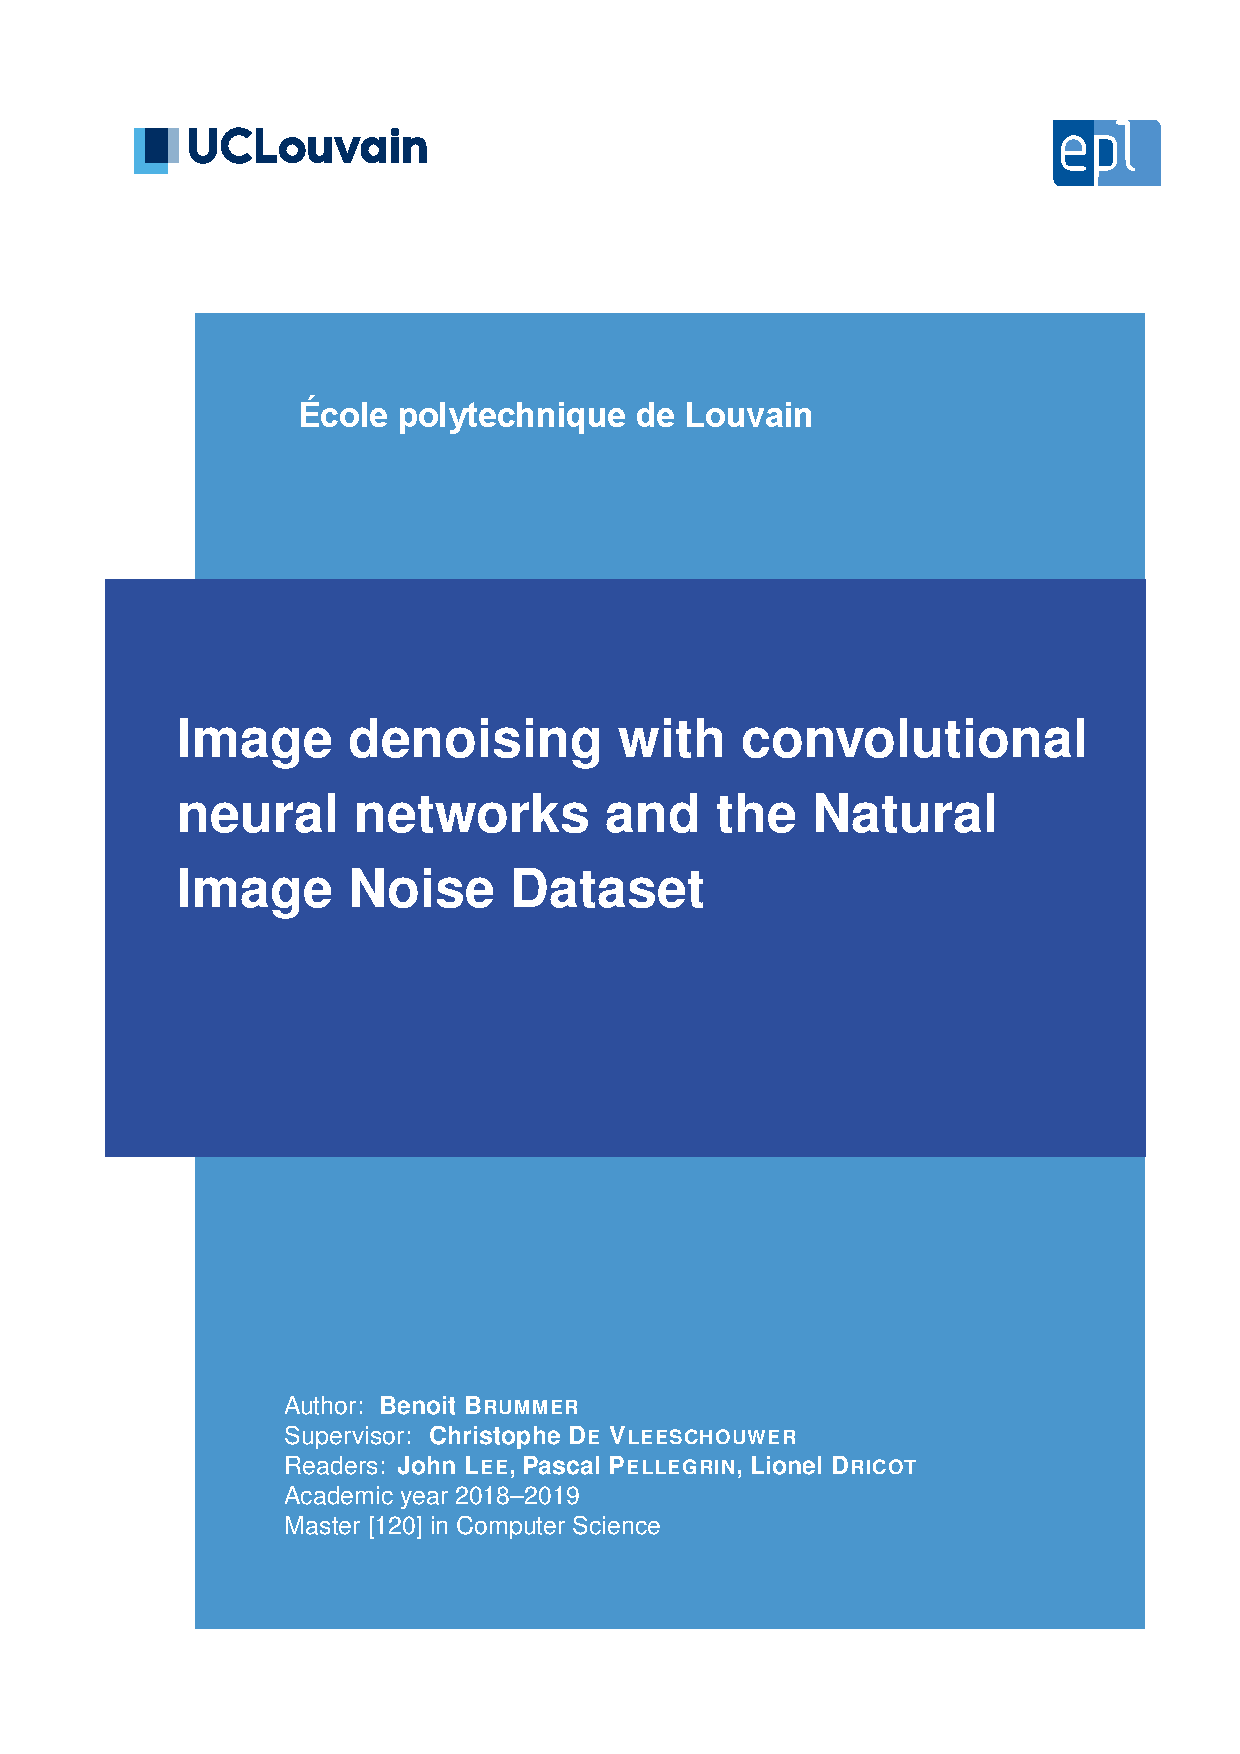
\includepdf{EPL-master-thesis-covers-template-EN.pdf}

%********************************************************************
% Bibliographies
%*******************************************************
\addbibresource{Bibliography.bib}
\addbibresource[label=ownpubs]{AMiede_Publications.bib}

%********************************************************************
% Hyphenation
%*******************************************************
%\hyphenation{put special hyphenation here}

% ********************************************************************
% GO!GO!GO! MOVE IT!
%*******************************************************
\begin{document}
\frenchspacing
\raggedbottom
\selectlanguage{american} % american ngerman
%\renewcommand*{\bibname}{new name}
%\setbibpreamble{}
\pagenumbering{roman}
\pagestyle{plain}
%********************************************************************
% Frontmatter
%*******************************************************
%%*******************************************************
% Little Dirty Titlepage
%*******************************************************
\thispagestyle{empty}
%\pdfbookmark[1]{Titel}{title}
%*******************************************************
\begin{center}
    \spacedlowsmallcaps{\myName} \\ \medskip

    \begingroup
        \color{CTtitle}\spacedallcaps{\myTitle}
    \endgroup
\end{center}

%%*******************************************************
% Titlepage
%*******************************************************
\begin{titlepage}
    %\pdfbookmark[1]{\myTitle}{titlepage}
    % if you want the titlepage to be centered, uncomment and fine-tune the line below (KOMA classes environment)
    \begin{addmargin}[-1cm]{-3cm}
    \begin{center}
        \large

        \hfill

        \vfill

        \begingroup
            \color{CTtitle}\spacedallcaps{\myTitle} \\ \bigskip
        \endgroup

        \spacedlowsmallcaps{\myName}

        \vfill

        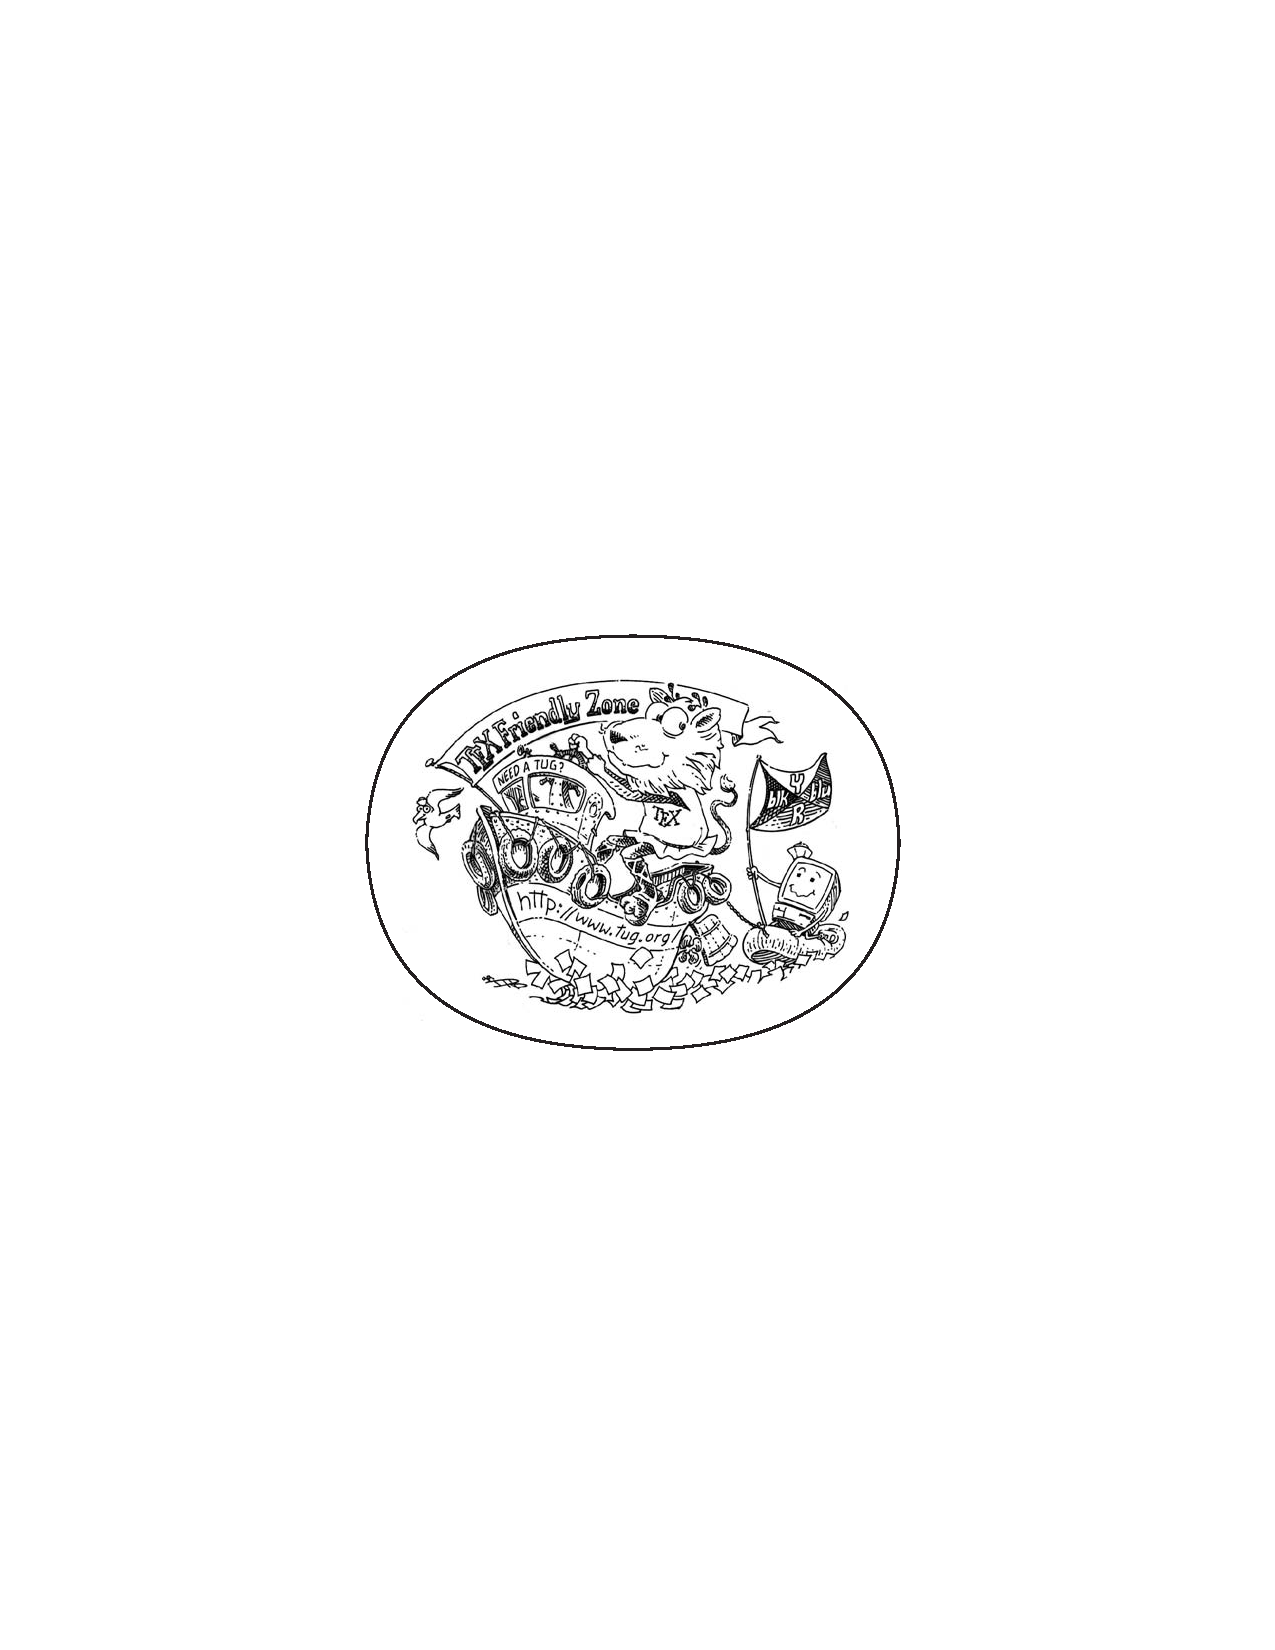
\includegraphics[width=6cm]{gfx/TFZsuperellipse_bw} \\ \medskip

        \mySubtitle \\ \medskip
        %\myDegree \\
        %\myDepartment \\
        %\myFaculty \\
        %\myUni \\ \bigskip

        \myTime\ -- \myVersion

        \vfill

    \end{center}
  \end{addmargin}
\end{titlepage}

%\thispagestyle{empty}

\hfill

\vfill

\noindent\myName: \textit{\myTitle,} \mySubtitle, %\myDegree,
\textcopyright\ \myTime

%\bigskip
%
%\noindent\spacedlowsmallcaps{Supervisors}: \\
%\myProf \\
%\myOtherProf \\
%\mySupervisor
%
%\medskip
%
%\noindent\spacedlowsmallcaps{Location}: \\
%\myLocation
%
%\medskip
%
%\noindent\spacedlowsmallcaps{Time Frame}: \\
%\myTime

%\cleardoublepage%*******************************************************
% Dedication
%*******************************************************
\thispagestyle{empty}
\phantomsection
\pdfbookmark[1]{Dedication}{Dedication}

\vspace*{3cm}

\begin{center}
    \emph{Ohana} means family. \\
    Family means nobody gets left behind, or forgotten. \\ \medskip
    --- Lilo \& Stitch
\end{center}

\medskip

\begin{center}
    Dedicated to the loving memory of Rudolf Miede. \\ \smallskip
    1939\,--\,2005
\end{center}

%\cleardoublepage\include{FrontBackmatter/Foreword}
\cleardoublepage%*******************************************************
% Abstract
%*******************************************************
%\renewcommand{\abstractname}{Abstract}
\pdfbookmark[1]{Abstract}{Abstract}
% \addcontentsline{toc}{chapter}{\tocEntry{Abstract}}
\begingroup
\let\clearpage\relax
\let\cleardoublepage\relax
\let\cleardoublepage\relax

\chapter*{Abstract}
%Short summary of the contents in English\dots a great guide by
%Kent Beck how to write good abstracts can be found here:
%\begin{center}
%\url{https://plg.uwaterloo.ca/~migod/research/beckOOPSLA.html}
%\end{center}


Convolutional neural networks have been the focus of research aiming to solve image denoising problems, but their performance remains unsatisfactory for most applications. These networks are trained with synthetic noise distributions that do not accurately reflect the noise captured by image sensors. Some datasets of clean-noisy image pairs have been introduced but they are usually meant for benchmarking or specific applications. We introduce the Natural Image Noise Dataset (NIND), a dataset of DSLR-like images with varying levels of ISO noise which is large enough to train models for blind denoising over a wide range of noise. We demonstrate the use of denoising models trained with the NIND and show that they significantly outperform BM3D on ISO noise from unseen images, even when generalizing to images from a different type of camera. We expect that this dataset will prove useful for future image denoising applications. Finally, we investigate the use of conditional generative adversarial networks (cGAN) which provide better denoising performance in some edge cases that a paired dataset may not cover, and we develop a framework which lays the groundwork to train such networks as well as a pair of discriminator-generator architectures that perform well in such systems.


\vfill

%\begin{otherlanguage}{ngerman}
%\pdfbookmark[1]{Zusammenfassung}{Zusammenfassung}
%\chapter*{Zusammenfassung}
%Kurze Zusammenfassung des Inhaltes in deutscher Sprache\dots
%\end{otherlanguage}

\endgroup

\vfill

%\cleardoublepage%*******************************************************
% Publications
%*******************************************************
\pdfbookmark[1]{Publications}{publications}
\chapter*{Publications}\graffito{This is just an early --~and currently ugly~-- test!}
This might come in handy for PhD theses: some ideas and figures have appeared previously in the following publications:

%\noindent Put your publications from the thesis here. The packages \texttt{multibib} or \texttt{bibtopic} etc. can be used to handle multiple different bibliographies in your document.

\begin{refsection}[ownpubs]
    \small
    \nocite{*} % is local to to the enclosing refsection
    \printbibliography[heading=none]
\end{refsection}

\emph{Attention}: This requires a separate run of \texttt{bibtex} for your \texttt{refsection}, \eg, \texttt{ClassicThesis1-blx} for this file. You might also use \texttt{biber} as the backend for \texttt{biblatex}. See also \url{http://tex.stackexchange.com/questions/128196/problem-with-refsection}.

%\cleardoublepage%*******************************************************
% Acknowledgments
%*******************************************************
\pdfbookmark[1]{Acknowledgments}{acknowledgments}

%\begin{flushright}{\slshape
%    We have seen that computer programming is an art, \\
%    because it applies accumulated knowledge to the world, \\
%    because it requires skill and ingenuity, and especially \\
%    because it produces objects of beauty.} \\ \medskip
%    --- \defcitealias{knuth:1974}{Donald E. Knuth}\citetalias{knuth:1974} \citep{knuth:1974}
%\end{flushright}



\bigskip

\begingroup
\let\clearpage\relax
\let\cleardoublepage\relax
\let\cleardoublepage\relax
\chapter*{Acknowledgments}
I would like to thank Christophe De Vleeschouwer for taking the time to meet with me every week, sharing a great deal of knowledge and ideas, and supporting my endeavors; Leslie Sanderson for proofreading my work and contributing to a happy and supportive work environment; the Wikimedia Commons QI community for providing constructive criticism which helped me improve my photographic skills to the point where this master thesis is of great relevance to my interests; and Larry the cat.
% Put your acknowledgments here.
%
% Many thanks to everybody who already sent me a postcard!
%
% Regarding the typography and other help, many thanks go to Marco
% Kuhlmann, Philipp Lehman, Lothar Schlesier, Jim Young, Lorenzo
% Pantieri and Enrico Gregorio\footnote{Members of GuIT (Gruppo
% Italiano Utilizzatori di \TeX\ e \LaTeX )}, J\"org Sommer,
% Joachim K\"ostler, Daniel Gottschlag, Denis Aydin, Paride
% Legovini, Steffen Prochnow, Nicolas Repp, Hinrich Harms,
% Roland Winkler, Jörg Weber, Henri Menke, Claus Lahiri,
% Clemens Niederberger, Stefano Bragaglia, Jörn Hees,
% Scott Lowe, Dave Howcroft, Jos\'e M. Alcaide, David Carlisle,
% Ulrike Fischer, Hugues de Lassus, Csaba Hajdu, Dave Howcroft, 
% and the whole \LaTeX-community for support, ideas and
% some great software.
%
% \bigskip
%
% \noindent\emph{Regarding \mLyX}: The \mLyX\ port was intially done by
% \emph{Nicholas Mariette} in March 2009 and continued by
% \emph{Ivo Pletikosi\'c} in 2011. Thank you very much for your
% work and for the contributions to the original style.


\endgroup

\cleardoublepage%*******************************************************
% Table of Contents
%*******************************************************
\pagestyle{scrheadings}
%\phantomsection
\pdfbookmark[1]{\contentsname}{tableofcontents}
\setcounter{tocdepth}{2} % <-- 2 includes up to subsections in the ToC
\setcounter{secnumdepth}{3} % <-- 3 numbers up to subsubsections
\manualmark
\markboth{\spacedlowsmallcaps{\contentsname}}{\spacedlowsmallcaps{\contentsname}}
\tableofcontents
\automark[section]{chapter}
\renewcommand{\chaptermark}[1]{\markboth{\spacedlowsmallcaps{#1}}{\spacedlowsmallcaps{#1}}}
\renewcommand{\sectionmark}[1]{\markright{\textsc{\thesection}\enspace\spacedlowsmallcaps{#1}}}
%*******************************************************
% List of Figures and of the Tables
%*******************************************************
\clearpage
% \pagestyle{empty} % Uncomment this line if your lists should not have any headlines with section name and page number
\begingroup
    \let\clearpage\relax
    \let\cleardoublepage\relax
    %*******************************************************
    % List of Figures
    %*******************************************************
    %\phantomsection
    %\addcontentsline{toc}{chapter}{\listfigurename}
    \pdfbookmark[1]{\listfigurename}{lof}
    \listoffigures

    \vspace{8ex}

    %*******************************************************
    % List of Tables
    %*******************************************************
    %\phantomsection
    %\addcontentsline{toc}{chapter}{\listtablename}
    \pdfbookmark[1]{\listtablename}{lot}
    \listoftables

    \vspace{8ex}
    % \newpage

    %*******************************************************
    % List of Listings
    %*******************************************************
    %\phantomsection
    %\addcontentsline{toc}{chapter}{\lstlistlistingname}
    \pdfbookmark[1]{\lstlistlistingname}{lol}
    \lstlistoflistings

    \vspace{8ex}

    %*******************************************************
    % Acronyms
    %*******************************************************
    %\phantomsection
    \pdfbookmark[1]{Acronyms}{acronyms}
    \markboth{\spacedlowsmallcaps{Acronyms}}{\spacedlowsmallcaps{Acronyms}}
    \chapter*{Acronyms}
    \begin{acronym}[UMLX]
    	\acro{NIND}{Natural Image Noise Dataset \cite{nind-wc}\cite{nind-ntire}}
    	\acro{BCE}{binary cross-entropy}
    	\acro{BM3D}{block-matching and 3D filtering \cite{bm3d}}
    	\acro{BN}{batch normalization \cite{bn}}
    	\acro{cGAN}{conditional generative adversarial network \cite{cgan}}
    	\acro{CNN}{convolutional neural network \cite{cnn}}
    	\acro{DSLR}{digital single-lens reflex}
    	\acro{DCGAN}{deep convolutional generative adversarial network\cite{dcgan}}
    	\acro{GAN}{generative adversarial network \cite{gan}}
    	\acro{LSGAN}{Least Squares Generative Adversarial Network \cite{lsgan}}
    	\acro{MSE}{mean squared error}
    	\acro{RED-Net}{very deep Residual Encoder-Decoder Network \cite{rednet}}
    	\acro{ReLU}{rectified linear unit \cite{relu}}
    	\acro{PReLU}{parametric rectified linear unit \cite{prelu}}
    	\acro{SIDD}{Smartphone Image Denoising Dataset \cite{sidd}}
    	\acro{SSIM}{Structural Similarity \cite{ssim}}
    	\acro{C500D}{Canon EOS 500D DSLR camera}
    	\acro{X-T1}{Fujifilm X-T1 mirrorless camera}
    	\acro{k}{\text{kernel size }}
    	\acro{p}{\text{padding size }}
    \end{acronym}

\endgroup

%********************************************************************
% Mainmatter
%*******************************************************
\cleardoublepage
\pagestyle{scrheadings}
\pagenumbering{arabic}
%\setcounter{page}{90}
% use \cleardoublepage here to avoid problems with pdfbookmark
\cleardoublepage
%\part{Some Kind of Manual}\label{pt:manual}
\chapter{Introduction}\label{chap:Introduction}

%begoldintro
% what is image noise
%\section{Image noise}
Photographic image noise occurs as a camera sensor's ISO sensitivity increases to capture an image faster than it would in ideal conditions (``base ISO" sensitivity).\footnote{We often make references to ISO noise because increased ISO sensitivity is the main cause of noise, but it should be noted that there are other factors affecting the magnitude of noise acquired by the image sensor.} A fast shutter speed is often necessary even though there is insufficient light, for instance with handheld photography where a slow shutter speed results in blur caused by the camera shake, or when a dynamic subject results in motion blur. Increasing the ISO setting is akin to linearly amplifying the value measured on each sensor cell. A small initial value that is amplified is less accurate and more prone to errors; this amplified value in turn makes up photographic noise. 

%\section{Denoising methods}
% how are images denoised
Denoising is typically seen as the inverse problem of recovering the latent clean image from its noisy observation \cite{rednet}. 
% ADD traditional methods

Photographic development usually incorporates a conventional denoising method such as non-local means \cite{nlm} or wavelets-based methods \cite{wavelets-denoising}, or a combination thereof, sometimes making use of prior information about a specific sensor's response to different ISO noise values. \cite{darktable-denoising}
% why don't I need to cite bm3d here?
\ac{BM3D} is a more powerful denoising method which has been used to benchmark newer techniques \cite{all-bm3d-benchmarks}, though it is seldom used in off-the-shelf software (presumably because of its high computational cost and the need to specify a $\gamma$ noise value parameter). 

The use of deep learning to solve the denoising problem by directly generating the latent clean image, or in some cases recreating the noise and subtracting it from the observed image \cite{dncnn}, has been an active research area. However, while the synthetic results show state-of-the-art performance, testing on real data indicates that neural network-based solutions do not exceed the performance offered by \ac{BM3D} \cite{darmstadt}. It appears that neural networks simply learn the applied noise distribution and that ISO noise may involve additional transformations such as color distortions and loss of detail.

Some specialized work has shown that neural networks obtain state-of-the-art performance when trained with real data \cite{learningtoseeinthedark}\cite{microscopynoise}. We sought to assess the potential of deep learning applied to the denoising problem by expanding on this previous work through a dataset of images produced with various levels of ISO noise. This dataset can be used to train neural network models for general purpose denoising of high quality images.

Our work introduces an open dataset of DSLR-like\footnote{\label{largesensornote}We define a DSLR-like camera as one produced with an APS-C (25.1x16.7 mm) or larger sensor such as those present in most DSLR and mirrorless cameras} image sets with various levels of real noise caused by the digital sensor's increased ISO sensitivity. The dataset is large enough to be used for training and varies in content in order to model a great variety of scenes. Each scene was captured at multiple noise levels, with an average of 6 images per set, such that a model may be trained for blind denoising on the base ISO as well as beyond the highest ISO value of the camera by feeding it crops that have a random noise value.

The images in a set are all pixel-aligned. Some of the scenes include multiple ground-truth images which may be sampled at random during training; these would prevent the model from learning to reconstruct the random noise it has seen on one ground-truth, thus making it more difficult to overfit the noise. Overexposed areas are avoided in the ground-truth images because details are lost when the sensor is saturated and this could potentially give an advantage to higher ISO images in which the sensor is not necessarily saturated (notably in ISO-invariant cameras and high ISO pictures that are brightened using software).

The dataset is published in sRGB format on Wikimedia Commons, which is an open-platform that promotes continuous discussion and contribution.

%ADDED
We trained several convolutional neural network architectures presented in the literature, namely DnCNN \cite{dncnn}, \ac{RED-Net}, and U-Net \cite{unet}, and analysed different proposed methods such as DnCNN \cite{dncnn}'s residual learning. 

In most tests a U-Net model was trained with the \ac{NIND} and validated over increasing ISO values; test sets were taken with the same Fujifilm X-T1, as well as a Canon EOS 500D DSLR camera to assess the generalization. We also attempted to combine other datasets with our training data to assess the potential loss in performance caused by generalization. %Do I need to list results here?% %We found good generalization which did not suffer a significant performance hit when compared to specialized models.
Finally we investigated the use of Generative Adversarial Networks\cite{pix2pix} to solve issues such as unnatural face smoothing.
%endoldintro

%what/why/how (short)

%~4-5 (up to 10) typical
%\section{Image noise}
%\section{Current methods}
%\section{Our work}

\cleardoublepage
%\ctparttext{You can put some informational part preamble text here.
%Illo principalmente su nos. Non message \emph{occidental} angloromanic
%da. Debitas effortio simplificate sia se, auxiliar summarios da que,
%se avantiate publicationes via. Pan in terra summarios, capital
%interlingua se que. Al via multo esser specimen, campo responder que
%da. Le usate medical addresses pro, europa origine sanctificate nos se.}
%\part{The Showcase}\label{pt:showcase}
\chapter{Dataset}\label{chap:Dataset}

The Dataset chapter goes over some existing image noise datasets before delving into the Natural Image Noise Dataset.

\section{Related work}
The following works feature datasets made of ground-truth / noisy image sets. The static scenes approach is necessary to directly compare the level of degradation using a loss function such as the \ac{SSIM} index or the \ac{MSE}. 
\subsection{Darmstadt Noise Dataset}
The Darmstadt Noise Dataset (DND) \cite{darmstadt}, containing 50 pairs of noisy-clean images from four cameras, was developed for the purpose of validating denoising algorithms using real data. Synthetic noise is typically used to train and test models, but it had been unclear whether the reported synthetic results translated to real improvements. Plötz and Roth showed that many modern denoising methods do not perform well on real data and that BM3D \cite{bm3d}, which was published in 2006, remains one of the best performing methods \cite{darmstadt}. RENOIR \cite{renoir} is a similar dataset that was published prior to the DND; however, Plötz and Roth noted spatial misalignments that reduced its effectivity. We have additionally found that the light sometimes differs between images in the same scene and that some photographs exhibit significant raw overexposure.
\subsection{Learning to See in the Dark}
See-in-the-Dark (SID) \cite{learningtoseeinthedark} is an image noise dataset that is large enough for training and, to our knowledge, was used in the first successful attempt at denoising images using real image noise. This dataset focused on very low-light photography where the camera-generated JPEG appears black. The authors used a U-Net network architecture to create an end-to-end RAW-to-JPEG pipeline that produces realistic colors, improving on standard processing and BM3D denoised images which still suffer from color bias at high ISO. Our work differs from SID in that we aimed to train a general purpose (``blind") denoiser rather than one that handles a specific condition, such as extremely low light images. We chose to work in sRGB space because handling the whole RAW-to-sRGB pipeline removes some information which may otherwise be useful to the author during development. Moreover, one dataset can then be used with different types of color filter arrays.
%raw-to-srgb (cons: removes freedom of photographer)
\subsection{Smartphone Image Denoising Dataset}
The Smartphone Image Denoising Dataset (SIDD) \cite{sidd} is comprised of 10 scenes * 5 cameras * 4 conditions * 150 images, totalling 30000 images. This dataset aims to address the problem of smartphone image denoising, where the small sensor and aperture size causes noticeable noise even in pictures taken at base ISO. Further processing is thus applied to create ground-truth images out of many images. This method of creating ground-truth images is not entirely relevant for denoising images captured with larger sensors because a single image taken at base ISO on a DSLR-like camera is clean enough to work as ground-truth for training purposes.
%\subsubsection{Network architectures}
%
%We initially trained a DnCNN\cite{dncnn} architecture which is 
%- rednet (and dncnn)
%- U-Net
% This probably doesn't belong here
\section{Natural Image Noise Dataset}

\marginpar{DRAFTy-as-heck sentence}
The Natural Image Noise Dataset fills the gap for an image noise dataset of ground-truth - noisy image sets that targets cameras equipped with larger sensors\footnoteref{largesensornote} and which is large and varied enough (in both noise values and content types) to train a denoising model for ISO-blind denoising.\marginpar{FIXME long run-on sentence}

Here we outline the physical setup required to capture image sets for the NIND, summarize its content, explain the software processing and validation requirements, and describe its publication aspects such that others that wish to do so may also contribute.
\subsection{Capture}
We captured several images per static scene; at least one ground-truth taken with the camera's lowest ISO setting and several images taken with increasing ISO settings and consequent decreasing shutter speed in order to match the original exposure value. Scenes were captured using a camera affixed to a tripod and controlled with a wireless remote control to avoid shifting the setup position. We ensured that the ground was stable, wind would not cause any change in the scene, lighting did not vary between shots, and no area was overexposed in the ground-truth images. Overexposure occurs when the sensor is saturated; on a ground-truth image this would potentially benefit the high ISO images because less light is captured with a faster shutter speed, therefore, the higher ISO images may not be overexposed and thus may contain detail that is not present in the overexposed ground-truth. The aperture remained the same on all shots and the focus was set manually so that it would not automatically adjusted for each frame.

A base ISO image (ISO200 on the Fujifilm X-T1) was always taken at least once, along with the camera's highest ISO setting (ISO6400 on the X-T1). Several images were taken with different intermediate ISO values such that the ISO settings varied across each scene. We often also took images that we categorized as ``High ISO," which consisted of the highest ISO value and increased shutter speed. ``High ISO" images result in dark frames which are then correctly exposed using software. We often tried to match shutter speeds that would be useful to denoise, such as 1/60s for handheld photography, 1/15s for devices equipped with optical image stabilization, and 1/1000s or faster for high-speed photography. We ensured that every ISO value was well represented in order to train models effective at blind denoising. On average, six images were produced per scene and some scenes featured multiple ground truth images which could be used in training to help prevent over-fitting.
\subsection{Content}
\begin{figure}
%\centering
%\fbox{\rule{0pt}{2in} \rule{.9\linewidth}{0pt}}
  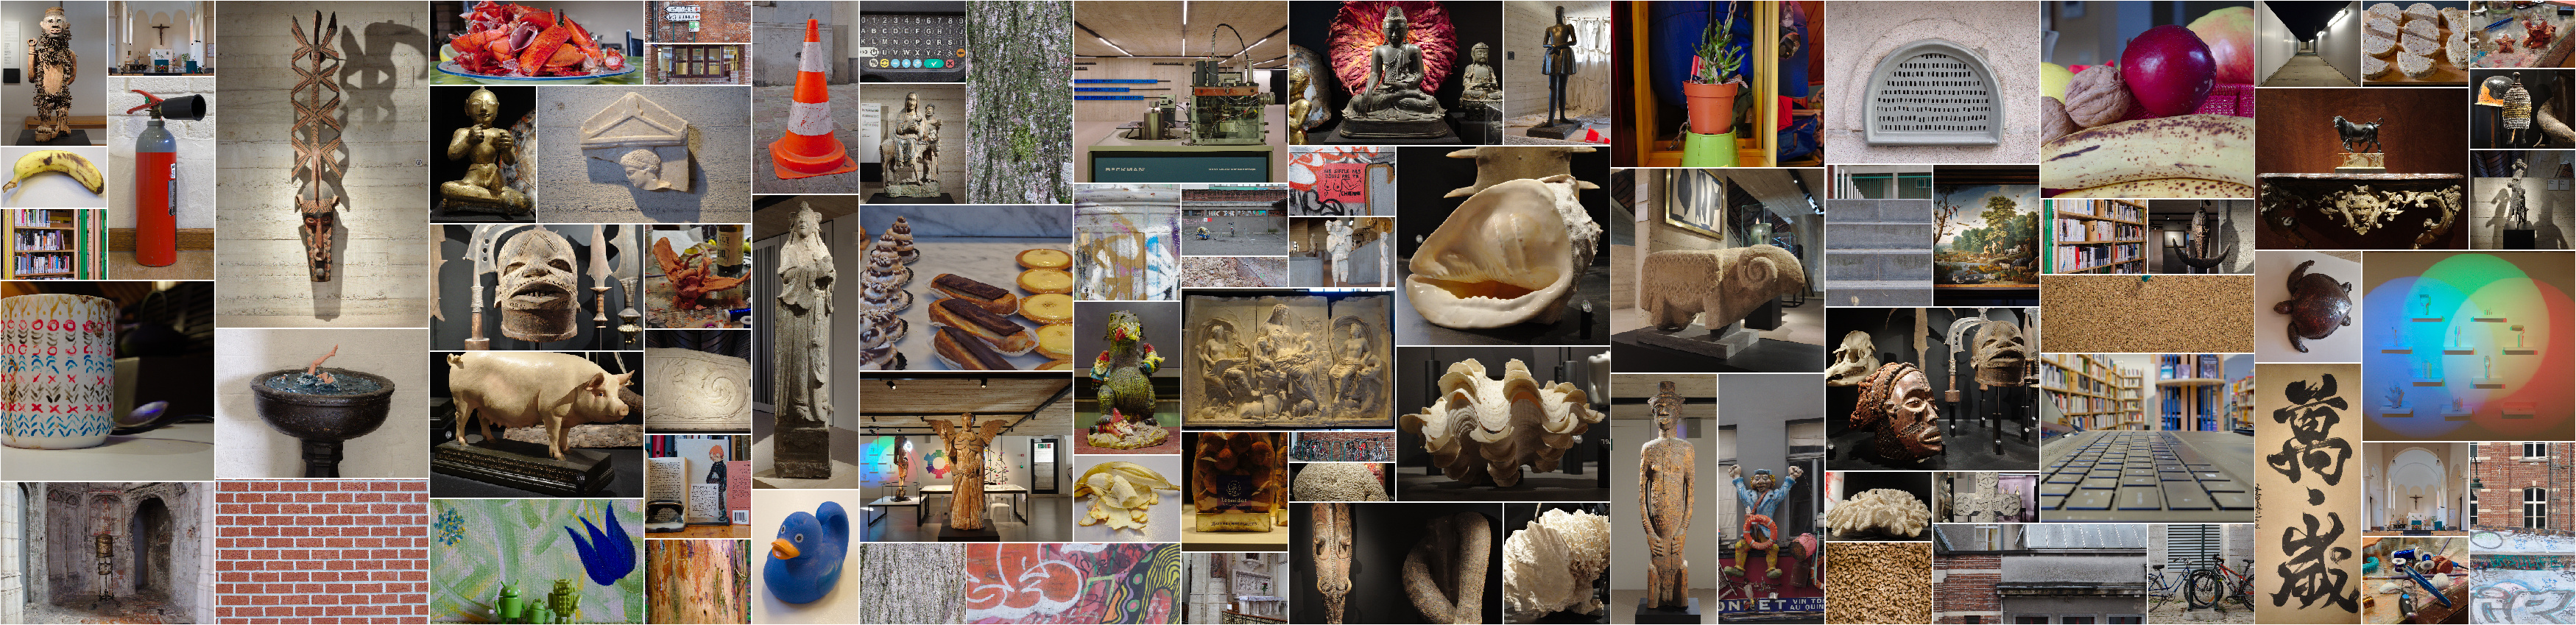
\includegraphics[width=1\linewidth]{gfx/samplebanner.jpg}
   \caption{Sample ground-truth images from the Natural Image Noise Dataset.}
%\vspace{-0.2cm} 
\label{fig:sampleimg}
\end{figure}

\begin{table}
%\centering
\resizebox{1\linewidth}{!}{
\begin{tabular}{lllllllllllllllllll|ll}
\ul{ISO value} & \ul{100} & \ul{200} & \ul{250} & \ul{320} & \ul{400} & \ul{500} & \ul{640} & \ul{800} & \ul{1000} & \ul{1250} & \ul{1600} & \ul{2000} & \ul{2500} & \ul{3200} & \ul{4000} & \ul{5000} & \ul{6400} & \ul{High} & \ul{Scenes} & \ul{Images} \\
\ul{Fujifilm X-T1}      &           & 105       & 11        & 8         & 18        & 13        & 16        & 25        & 16         & 9          & 12         & 9          & 19         & 25         & 17         & 19         & 91         & 123        & 90         & 536          \\
\ul{Canon C500D}     & 14        & 10        &           &           & 10        &           &           & 10        &            &            & 9          &            &            & 11         &            &            &            & 10         & 11         & 74           \\ \hline
\ul{Total}     & 15        & 116       & 11        & 8         & 29        & 13        & 16        & 36        & 16         & 9          & 22         & 9          & 19         & 37         & 17         & 19         & 91         & 133        & 101        & 616         
\end{tabular}%
}
\caption{Dataset content}
% \vspace{-0.2cm} 
\label{tableDSContent}
\end{table}

% TODO compute noise value on these
Many objects were captured in museums where subjects are plentiful (albeit we had to be mindful of copyright restricted material) and for which a denoising application would be highly relevant because indoor handheld pictures require a high ISO sensitivity. However, initial tests found that using images taken only indoors did not provide the variety needed to create a model that generalized well across all conditions, as natural colors were sometimes off in outdoor and brightly lit applications. We thus captured natural objects with vibrant colors (such as food items and plant-life) as well as outdoor scenes where the shutter speed could be taken as fast as 1/13000s using a digital shutter. We made an effort to include some text because it is prevalent, yet we expect a model would not be able to guess how to reconstruct it (Figure \ref{fig:text} shows the resulting denoised text), and we tried to make the images pleasant to look at in order to enhance the time users would spend looking at them. Most of the NIND images were captured on a Fujifilm X-T1 mirrorless camera, which uses a 23.6 x 15.6 mm X-Trans sensor. A Canon EOS 500D DSLR camera, featuring a 22.3 x 14.9 mm standard Bayer sensor, was used to capture images that could be used to validate the generalization. The content of the dataset is summarized in Table \ref{tableDSContent} and a subset of the X-T1 pictures are shown in Figure \ref{fig:sampleimg}.
\subsection{Software processing}
We processed the dataset images using darktable \cite{darktable} (an open source development software) for raw-to-sRGB development. Our development steps are similar to those we would apply to a standard picture but no sharpening was applied, as this greatly amplifies noise and is typically applied last in the pixel pipeline (we can expect users to apply sharpening to the generated clean image without any perceptible loss). We used darktable's automatic exposure mode to match a fixed percentile target on the histogram and calculate the required exposure compensation for all images in a set. Likewise, we ensured that the white balance was identical and all development steps were copied over to the entire scene. (The exposure percentile and white balance settings are fixed within a scene but vary across different scenes.) The raw overexposed indicator was used to verify that no overexposed areas were present in the base ISO image and if any were detected then it was cropped out or the scene was discarded. The images were visually inspected to detect slight variations in light, the introduction of foreign objects such as insects, or any movement, which also resulted in cropping or discarding images. The ground-truth images must be at least as sharp as their noisy counterparts; this is sometimes not the case due to slight movements on longer exposures. The remaining images were saved in either high-quality (98 to 100) 8-bit JPEG or lossless 16-bit PNG.

The last step of development is to use Hugin's align\_image\_stack tool \cite{hugin} to ensure that all images in a set are perfectly pixel-aligned. The tool will usually return the same image size as the input, in which case the whole image set can safely be used. When a difference is detected then the tool will automatically align the set and we visually analyzed whether the result was acceptable or the movement caused a change in perspective, in which case the outlier images were discarded. Some noisy images cannot easily be matched to the scene; possible solutions are to denoise these images in order to check the alignment or to take a cleaner image afterward and assume that the middle images are consistent with the previous and next ones.
\subsection{Publishing}
The Natural Image Noise Dataset is published on Wikimedia Commons ( \url{https://commons.wikimedia.org/wiki/Natural_Image_Noise_Dataset} ), an online repository of free-use images and other digital media. Wikimedia Commons hosts media content for all Wikimedia projects and its scope is limited only by the content having some educational value (broadly meaning ``providing knowledge; instructional or informative"). As such, we believe it is a fitting platform for the publication of a research dataset.

One key advantage of using Wikimedia Commons is its collaborative aspect. Anyone is allowed to add images to the dataset, modify existing images (for example to fix a spatial misalignment), and discuss the content (through the discussion page provided for each file, category, and the dataset itself). The collaborative aspect also includes a ``Quality images candidates" page \cite{qic} where users assess the technical quality of a submitted image and may promote it to a ``Quality image" standing. Many of the ground-truth images have gone through this process and were promoted through human assessment. The same process was also used to validate the trained model, which ended up in a positive assessment since even the denoised dynamic ISO6400 picture presented in Figure \ref{fig:visualpigeons} was among the promoted images.

On the technical side, Wikimedia Commons preserves images as they are uploaded; JPEG images are not recompressed, 16-bit lossless TIFF and PNG images are allowed, and the metadata is kept. Thumbnails are generated and images may be visualized before being downloaded in full resolution, and the download may include a select subset instead of the whole dataset. A customizable download script is provided on the dataset's page for convenient retrieval. Even though files can be overwritten, every file uploaded on Wikimedia Commons is kept forever therefore specific snapshots of the dataset can be made by including the files' revision in the download script and getting a specific version ID (or commit hash) of the download script.

It is also important to note the usefulness of the data outside of a denoising dataset context. Many images, such as those depicting artifacts displayed in churches and museums, have encyclopedic value and the ground-truth images present in our dataset are of higher quality than most previously available images depicting such artifacts. By publishing the dataset on Wikimedia Commons, these ground-truth images may be used in Wikipedia articles directly\footnote{E.g. \href{https://en.wikipedia.org/wiki/Bobo_people}{Bobo people}, \href{https://en.wikipedia.org/wiki/Bombardment_of_Brussels}{Bombardment of Brussels}, \href{https://en.wikipedia.org/wiki/Dengese_people}{Dengese people}}. This may be a motivating factor to those wishing to contribute.

%\addtocontents{toc}{\protect\clearpage} % <--- just debug stuff, ignore
\chapter{Generative Neural Networks}\label{chap:Arch1}
We use generative neural networks to generate denoised images from their noisy representation and thus solve the denoising problem. The class of generative network used to complete this task is a convolutional neural network. We introduces the notion of a \acl{CNN} and its components in section \ref{sec:Convolutional neural networks}, then section \ref{sec:Generative network architectures} goes over each specific network architecture we have worked with. All networks presented is this chapter are generative; a generative network takes an image of $W\times H$ pixels with three channels and generates a new image of the same dimensions. It differs from other types of \aclp{CNN} which have different output shapes, for example a classification network (such as those used in chapter \ref{chap:Arch2}) outputs one to a few probabilities, and segmentation networks usually have the same height and width dimensions as the input image but one channel per segmented feature (segmentation networks can easily be adapted into generative models as is the case for U-Net \cite{unet}). 

\section{Convolutional neural networks}\label{sec:Convolutional neural networks}
%- Introduce convolutional neural networks

We use deep convolutional neural networks which are neural networks based on the multilayer perceptron; that is, input data from one layer is sent to the neurons of the next layer and a dot product is performed between that input data and the next layer's learned weights. This process goes on for each layer. The main difference between a multilayer perceptron and a \ac{CNN} is that a \ac{CNN} is not fully connected so neurons in one layer only receive a subset of the previous layer's neurons. Instead, a \ac{CNN} takes advantage of the local spatial coherence of the input images to share weights and thus reduce the number of shared parameters. This process is shown in figure \ref{fig:convolutionfilter} where one filter is applied across the previous (in this case first) layer to create one channel of the following layer.

% plural?
The first and last layer of a generative network have the same shape as the input image, that is its height, width, and 3-channels representing the RGB color-space. Most layers in a deep network are hidden layers between the first and last one. Hidden layers contain many more channels (also called feature maps), they are usually convolution (or transposed convolution) layers, activation layers, or pooling layers.

A loss function is applied to the output of the last layer, its gradient with respect to the network's weights is calculated with the backpropagation algorithm, and the Adam gradient-descent algorithm\cite{adam} (the optimizer) adjusts the weights at the end of each batch training iteration. The optimizer's learning rate needs to be fine-tuned in order to optimize fast learning without over-fitting.

\subsection{Layers}

\begin{figure}
  \begin{center}
    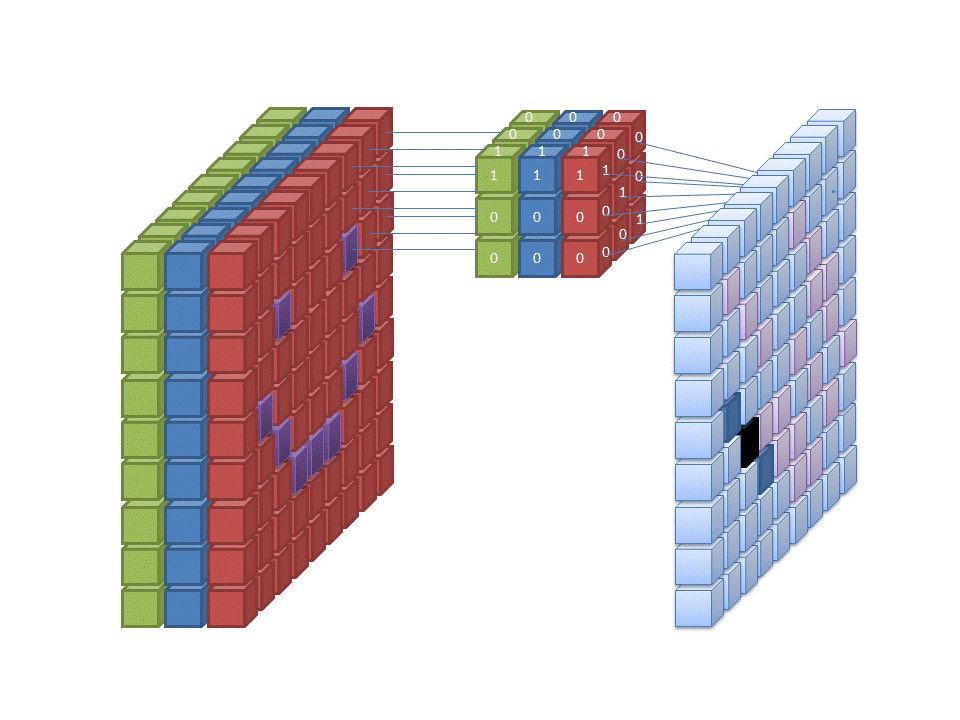
\includegraphics{gfx/Convolutional_Neural_Network_with_Color_Image_Filter.png}
    \caption[Standard convolution]{A filter is applied to the first 3-channels (RGB) input of an image in a convolutional neural network. The same filter is applied across all channels of the whole image as shown, and many of these filters are applied to form the following layer's feature map (i.e. its channels). Illustration by Wikimedia Commons user \href{https://commons.wikimedia.org/wiki/File:Convolutional_Neural_Network_with_Color_Image_Filter.gif}{Cecbur} (\href{https://creativecommons.org/licenses/by-sa/4.0/deed.en}{CC-BY-SA-4.0} license)}
    \label{fig:convolutionfilter}
  \end{center}
\end{figure}

\textbf{Convolution layers} apply convolutions with $C$ filters (also called features) to every $\acs{k}*\acs{k}$ area in the previous layer's width and height\footnote{assuming a stride of 1}, taking in every channel and returning one value per filter. Convolutions have a receptive field that is determined by \ac{k} whose typical values are 3 or 5. The next layer's width and height is thus reduced unless padding is applied. Given an input layer's width or height dimension $d$ and \ac{p}, a convolution layer's output size can be calculated as $d-\ac{k}+2\ac{p}+1$. Each filter is weighted and weights are learned parameters. The same stack of filters is applied on every $\ac{k}*\ac{k}$ area of a given layer; therefore, \acp{CNN} have largely reduced number of weight parameters.

\textbf{Activation layers} introduce non-linearity; they apply an activation function to every value in the previous layer and the resulting layer has the same shape as its input layer. We use the Sigmoid ($\phi(z)={1\over{1+e^{-z}}}$) which constrains its input values between 0 and 1, and (parametric) \ac{ReLU} ($R(z)=\max(0,z)$) as activation functions. 

% add gradient descent, BN

\subsection{Loss function}
% therefore and however are not interchangeable but they are used the same way with the punctuation sort of like that yeah they should never have as pace on either side words
The loss function assigns a score to the generated images with respect to the provided ground-truth. A loss function should not simply compare the difference between generated and ground-truth pixels because there is no one-to-one mapping between clean and noisy images. Therefore, a loss function which only focuses on the difference between pixels favors denoised images whose pixels average the many acceptable values; i.e. the network is trained to generate blurry images. \cite{pix2pix}

The \ac{MSE} (or $\ell 2$ loss) measures the average squared difference between the generated and ground-truth pixels \newline($MSE(\text{generated}, \text{ground-truth})=\sum_p^\text{pixels}{(\text{generated}_p-\text{ground-truth}_p)^2\over{|\text{pixels}|}}$), it is a simple yet effective loss function. Similarly, the $\ell 1$ loss measures the sum of the absolute differences between ground-truth and generated pixels; this typically favors blurrier results. The \ac{SSIM} index is another metric which puts weights on structural information that is more likely to be perceived in images, namely local changes in luminance, contrast, and structure. A loss may also be learned such as the discriminator in an \acl{GAN}.

%https://arxiv.org/pdf/1511.08861.pdf
Mixing different losses often appears to yield better results \cite{lossescomp}, although it is sometimes challenging to combine them because they are often scaled differently (and training may suffer a performance penalty when having to compute multiple losses). Another valid approach is to switch loss function once convergence has been attained with one. \cite{lossescomp} We typically use the \ac{SSIM} index in our standard models and a combination of loss functions in the more challenging \ac{GAN}.

%\marginpar{TODO: batch normalization}

\section{Generative network architectures}\label{sec:Generative network architectures}
\subsection{DnCNN}
DnCNN is a simple flat \ac{CNN} architecture introduced by Zhang et al. \cite{dncnn} to denoise images with residual learning. The network performs end-to-end denoising using only a convolution layer followed by \acl{BN} and a \ac{ReLU} activation layer at each depth level. The dimensions of the layers remain constant because the convolutions are padded appropriately ($\ac{p}={\ac{k}-1\over{2}}$). %The authors used a depth of 20 for blind gaussian denoising and set $\ac{k}=3$

The main contribution introduced in \cite{dncnn} appears to be the use of residual learning to speed up learning by modeling and subtracting the residual noise rather than generating a clean image. The use of a simple DnCNN architecture may have been introduced to emphasize the effectiveness of residual learning. DnCNN is the first network we experimented with because of its simplicity, and although most of our experiment focus on the subsequent networks, we tested the author's residual learning theory with our dataset of ISO noise in order to assess whether it would yield any gain in performance.
\subsection{RED-Net}
The \ac{RED-Net} architecture is a deep encoder-decoder network with residual skip connections \cite{rednet}. We found this type of network offers significantly better denoising performance and faster convergence than the DnCNN model. The first half of the network encodes the image using convolutions without padding such that the layers' dimensions continuously decrease, then the second half of the network (decoder) is made of transposed convolution layers that increase the layers' dimensions up to the original image's height and width. A \ac{ReLU} activation layer is placed between every (de)convolution layer. What is referred to as a residual network differs from the residual learning in Zhang et al. \cite{dncnn}. A residual network has skip connections which in the case of \ac{RED-Net} are placed every two convolution layers and connect them to transposed convolution layers of matching dimensions. These skip connections add details that may have been lost in the encoding process to the output of the transposed convolutions. 
\subsection{U-Net}
The U-Net architecture is an encoder-decoder with skip connections originally designed for image segmentation. Its use in an image generator is possible by using the number of input color channels as output features and upsampling the resulting image. Each U-Net block applies two 3x3 convolutions followed by a parameter-free pooling operation that downsamples the image by a factor of two. The first block has 64 filters and the number of filters doubles after every pooling operation until there are 1024 filters. From this point the downsampling pooling operations are replaced with 2x2 upsampling transposed convolutions and the number of filters get halved every time, but the convolutions remain (as opposed to using transposed convolutions) so the layers' size remain smaller on the upsampling stage than it is originally. This design results in corrupted borders which need to be discarded. The U-Net architecture uses significantly less resources than conventional encoder-decoder networks and it is able to capture details at multiple frequencies.
\subsection{HulbNet}\label{sec:HulbNet}
We designed a multi-scale architecture somewhat similar to U-Net whose aim is to be more adapted to the denoising problem at hand. HulbNet uses the following concepts:
\begin{figure}
  \begin{center}
    \animategraphics[width=\textwidth/3*2]{1}{gfx/dilation/frame-}{0}{8}
    \caption[Dilated convolution]{Dilated convolution (dilation=2). Illustration by GitHub user \href{https://github.com/vdumoulin/conv\_arithmetic}{vdumoulin} (\href{https://github.com/vdumoulin/conv\_arithmetic/blob/master/LICENSE}{MIT} license)}
    \label{fig:dilated}
  \end{center}
\end{figure}
\begin{figure}
  \begin{center}
  % Graphic for TeX using PGF
% Title: /orb/Dev/mthesis-denoise/thesis/gfx/convstr3.dia
% Creator: Dia v0.97.3
% CreationDate: Sun May 19 19:55:18 2019
% For: trougnouf
% \usepackage{tikz}
% The following commands are not supported in PSTricks at present
% We define them conditionally, so when they are implemented,
% this pgf file will use them.
\ifx\du\undefined
  \newlength{\du}
\fi
\setlength{\du}{15\unitlength}
\begin{tikzpicture}
\pgftransformxscale{1.000000}
\pgftransformyscale{-1.000000}
\definecolor{dialinecolor}{rgb}{0.000000, 0.000000, 0.000000}
\pgfsetstrokecolor{dialinecolor}
\definecolor{dialinecolor}{rgb}{1.000000, 1.000000, 1.000000}
\pgfsetfillcolor{dialinecolor}
\pgfsetlinewidth{0.100000\du}
\pgfsetdash{}{0pt}
\pgfsetdash{}{0pt}
\pgfsetmiterjoin
\definecolor{dialinecolor}{rgb}{0.000000, 0.501961, 0.000000}
\pgfsetfillcolor{dialinecolor}
\fill (28.000000\du,10.000000\du)--(28.000000\du,11.000000\du)--(29.000000\du,11.000000\du)--(29.000000\du,10.000000\du)--cycle;
\definecolor{dialinecolor}{rgb}{0.000000, 0.000000, 0.000000}
\pgfsetstrokecolor{dialinecolor}
\draw (28.000000\du,10.000000\du)--(28.000000\du,11.000000\du)--(29.000000\du,11.000000\du)--(29.000000\du,10.000000\du)--cycle;
\pgfsetlinewidth{0.100000\du}
\pgfsetdash{}{0pt}
\pgfsetdash{}{0pt}
\pgfsetmiterjoin
\definecolor{dialinecolor}{rgb}{0.501961, 0.000000, 0.501961}
\pgfsetfillcolor{dialinecolor}
\fill (28.000000\du,11.000000\du)--(28.000000\du,12.000000\du)--(29.000000\du,12.000000\du)--(29.000000\du,11.000000\du)--cycle;
\definecolor{dialinecolor}{rgb}{0.000000, 0.000000, 0.000000}
\pgfsetstrokecolor{dialinecolor}
\draw (28.000000\du,11.000000\du)--(28.000000\du,12.000000\du)--(29.000000\du,12.000000\du)--(29.000000\du,11.000000\du)--cycle;
\pgfsetlinewidth{0.100000\du}
\pgfsetdash{}{0pt}
\pgfsetdash{}{0pt}
\pgfsetmiterjoin
\definecolor{dialinecolor}{rgb}{0.678431, 0.847059, 0.901961}
\pgfsetfillcolor{dialinecolor}
\fill (28.000000\du,12.000000\du)--(28.000000\du,13.000000\du)--(29.000000\du,13.000000\du)--(29.000000\du,12.000000\du)--cycle;
\definecolor{dialinecolor}{rgb}{0.000000, 0.000000, 0.000000}
\pgfsetstrokecolor{dialinecolor}
\draw (28.000000\du,12.000000\du)--(28.000000\du,13.000000\du)--(29.000000\du,13.000000\du)--(29.000000\du,12.000000\du)--cycle;
\pgfsetlinewidth{0.100000\du}
\pgfsetdash{}{0pt}
\pgfsetdash{}{0pt}
\pgfsetmiterjoin
\definecolor{dialinecolor}{rgb}{0.901961, 0.901961, 0.980392}
\pgfsetfillcolor{dialinecolor}
\fill (28.000000\du,13.000000\du)--(28.000000\du,14.000000\du)--(29.000000\du,14.000000\du)--(29.000000\du,13.000000\du)--cycle;
\definecolor{dialinecolor}{rgb}{0.000000, 0.000000, 0.000000}
\pgfsetstrokecolor{dialinecolor}
\draw (28.000000\du,13.000000\du)--(28.000000\du,14.000000\du)--(29.000000\du,14.000000\du)--(29.000000\du,13.000000\du)--cycle;
\pgfsetlinewidth{0.100000\du}
\pgfsetdash{}{0pt}
\pgfsetdash{}{0pt}
\pgfsetmiterjoin
\definecolor{dialinecolor}{rgb}{0.647059, 0.164706, 0.164706}
\pgfsetfillcolor{dialinecolor}
\fill (29.000000\du,13.000000\du)--(29.000000\du,14.000000\du)--(30.000000\du,14.000000\du)--(30.000000\du,13.000000\du)--cycle;
\definecolor{dialinecolor}{rgb}{0.000000, 0.000000, 0.000000}
\pgfsetstrokecolor{dialinecolor}
\draw (29.000000\du,13.000000\du)--(29.000000\du,14.000000\du)--(30.000000\du,14.000000\du)--(30.000000\du,13.000000\du)--cycle;
\pgfsetlinewidth{0.100000\du}
\pgfsetdash{}{0pt}
\pgfsetdash{}{0pt}
\pgfsetmiterjoin
\definecolor{dialinecolor}{rgb}{0.545098, 0.411765, 0.078431}
\pgfsetfillcolor{dialinecolor}
\fill (30.000000\du,13.000000\du)--(30.000000\du,14.000000\du)--(31.000000\du,14.000000\du)--(31.000000\du,13.000000\du)--cycle;
\definecolor{dialinecolor}{rgb}{0.000000, 0.000000, 0.000000}
\pgfsetstrokecolor{dialinecolor}
\draw (30.000000\du,13.000000\du)--(30.000000\du,14.000000\du)--(31.000000\du,14.000000\du)--(31.000000\du,13.000000\du)--cycle;
\pgfsetlinewidth{0.100000\du}
\pgfsetdash{}{0pt}
\pgfsetdash{}{0pt}
\pgfsetmiterjoin
\definecolor{dialinecolor}{rgb}{0.564706, 0.933333, 0.564706}
\pgfsetfillcolor{dialinecolor}
\fill (31.000000\du,13.000000\du)--(31.000000\du,14.000000\du)--(32.000000\du,14.000000\du)--(32.000000\du,13.000000\du)--cycle;
\definecolor{dialinecolor}{rgb}{0.000000, 0.000000, 0.000000}
\pgfsetstrokecolor{dialinecolor}
\draw (31.000000\du,13.000000\du)--(31.000000\du,14.000000\du)--(32.000000\du,14.000000\du)--(32.000000\du,13.000000\du)--cycle;
\pgfsetlinewidth{0.100000\du}
\pgfsetdash{}{0pt}
\pgfsetdash{}{0pt}
\pgfsetmiterjoin
\definecolor{dialinecolor}{rgb}{1.000000, 0.000000, 0.000000}
\pgfsetfillcolor{dialinecolor}
\fill (15.000000\du,5.000000\du)--(15.000000\du,6.000000\du)--(16.000000\du,6.000000\du)--(16.000000\du,5.000000\du)--cycle;
\definecolor{dialinecolor}{rgb}{0.000000, 0.000000, 0.000000}
\pgfsetstrokecolor{dialinecolor}
\draw (15.000000\du,5.000000\du)--(15.000000\du,6.000000\du)--(16.000000\du,6.000000\du)--(16.000000\du,5.000000\du)--cycle;
\pgfsetlinewidth{0.100000\du}
\pgfsetdash{}{0pt}
\pgfsetdash{}{0pt}
\pgfsetmiterjoin
\definecolor{dialinecolor}{rgb}{1.000000, 0.000000, 0.000000}
\pgfsetfillcolor{dialinecolor}
\fill (16.000000\du,5.000000\du)--(16.000000\du,6.000000\du)--(17.000000\du,6.000000\du)--(17.000000\du,5.000000\du)--cycle;
\definecolor{dialinecolor}{rgb}{0.000000, 0.000000, 0.000000}
\pgfsetstrokecolor{dialinecolor}
\draw (16.000000\du,5.000000\du)--(16.000000\du,6.000000\du)--(17.000000\du,6.000000\du)--(17.000000\du,5.000000\du)--cycle;
\pgfsetlinewidth{0.100000\du}
\pgfsetdash{}{0pt}
\pgfsetdash{}{0pt}
\pgfsetmiterjoin
\definecolor{dialinecolor}{rgb}{1.000000, 0.000000, 0.000000}
\pgfsetfillcolor{dialinecolor}
\fill (17.000000\du,5.000000\du)--(17.000000\du,6.000000\du)--(18.000000\du,6.000000\du)--(18.000000\du,5.000000\du)--cycle;
\definecolor{dialinecolor}{rgb}{0.000000, 0.000000, 0.000000}
\pgfsetstrokecolor{dialinecolor}
\draw (17.000000\du,5.000000\du)--(17.000000\du,6.000000\du)--(18.000000\du,6.000000\du)--(18.000000\du,5.000000\du)--cycle;
\pgfsetlinewidth{0.100000\du}
\pgfsetdash{}{0pt}
\pgfsetdash{}{0pt}
\pgfsetmiterjoin
\definecolor{dialinecolor}{rgb}{0.000000, 1.000000, 0.000000}
\pgfsetfillcolor{dialinecolor}
\fill (18.000000\du,5.000000\du)--(18.000000\du,6.000000\du)--(19.000000\du,6.000000\du)--(19.000000\du,5.000000\du)--cycle;
\definecolor{dialinecolor}{rgb}{0.000000, 0.000000, 0.000000}
\pgfsetstrokecolor{dialinecolor}
\draw (18.000000\du,5.000000\du)--(18.000000\du,6.000000\du)--(19.000000\du,6.000000\du)--(19.000000\du,5.000000\du)--cycle;
\pgfsetlinewidth{0.100000\du}
\pgfsetdash{}{0pt}
\pgfsetdash{}{0pt}
\pgfsetmiterjoin
\definecolor{dialinecolor}{rgb}{0.000000, 1.000000, 0.000000}
\pgfsetfillcolor{dialinecolor}
\fill (19.000000\du,5.000000\du)--(19.000000\du,6.000000\du)--(20.000000\du,6.000000\du)--(20.000000\du,5.000000\du)--cycle;
\definecolor{dialinecolor}{rgb}{0.000000, 0.000000, 0.000000}
\pgfsetstrokecolor{dialinecolor}
\draw (19.000000\du,5.000000\du)--(19.000000\du,6.000000\du)--(20.000000\du,6.000000\du)--(20.000000\du,5.000000\du)--cycle;
\pgfsetlinewidth{0.100000\du}
\pgfsetdash{}{0pt}
\pgfsetdash{}{0pt}
\pgfsetmiterjoin
\definecolor{dialinecolor}{rgb}{0.000000, 1.000000, 0.000000}
\pgfsetfillcolor{dialinecolor}
\fill (20.000000\du,5.000000\du)--(20.000000\du,6.000000\du)--(21.000000\du,6.000000\du)--(21.000000\du,5.000000\du)--cycle;
\definecolor{dialinecolor}{rgb}{0.000000, 0.000000, 0.000000}
\pgfsetstrokecolor{dialinecolor}
\draw (20.000000\du,5.000000\du)--(20.000000\du,6.000000\du)--(21.000000\du,6.000000\du)--(21.000000\du,5.000000\du)--cycle;
\pgfsetlinewidth{0.100000\du}
\pgfsetdash{}{0pt}
\pgfsetdash{}{0pt}
\pgfsetmiterjoin
\definecolor{dialinecolor}{rgb}{0.000000, 0.000000, 1.000000}
\pgfsetfillcolor{dialinecolor}
\fill (21.000000\du,5.000000\du)--(21.000000\du,6.000000\du)--(22.000000\du,6.000000\du)--(22.000000\du,5.000000\du)--cycle;
\definecolor{dialinecolor}{rgb}{0.000000, 0.000000, 0.000000}
\pgfsetstrokecolor{dialinecolor}
\draw (21.000000\du,5.000000\du)--(21.000000\du,6.000000\du)--(22.000000\du,6.000000\du)--(22.000000\du,5.000000\du)--cycle;
\pgfsetlinewidth{0.100000\du}
\pgfsetdash{}{0pt}
\pgfsetdash{}{0pt}
\pgfsetmiterjoin
\definecolor{dialinecolor}{rgb}{0.000000, 0.000000, 1.000000}
\pgfsetfillcolor{dialinecolor}
\fill (22.000000\du,5.000000\du)--(22.000000\du,6.000000\du)--(23.000000\du,6.000000\du)--(23.000000\du,5.000000\du)--cycle;
\definecolor{dialinecolor}{rgb}{0.000000, 0.000000, 0.000000}
\pgfsetstrokecolor{dialinecolor}
\draw (22.000000\du,5.000000\du)--(22.000000\du,6.000000\du)--(23.000000\du,6.000000\du)--(23.000000\du,5.000000\du)--cycle;
\pgfsetlinewidth{0.100000\du}
\pgfsetdash{}{0pt}
\pgfsetdash{}{0pt}
\pgfsetmiterjoin
\definecolor{dialinecolor}{rgb}{0.000000, 0.000000, 1.000000}
\pgfsetfillcolor{dialinecolor}
\fill (23.000000\du,5.000000\du)--(23.000000\du,6.000000\du)--(24.000000\du,6.000000\du)--(24.000000\du,5.000000\du)--cycle;
\definecolor{dialinecolor}{rgb}{0.000000, 0.000000, 0.000000}
\pgfsetstrokecolor{dialinecolor}
\draw (23.000000\du,5.000000\du)--(23.000000\du,6.000000\du)--(24.000000\du,6.000000\du)--(24.000000\du,5.000000\du)--cycle;
\pgfsetlinewidth{0.100000\du}
\pgfsetdash{}{0pt}
\pgfsetdash{}{0pt}
\pgfsetmiterjoin
\definecolor{dialinecolor}{rgb}{1.000000, 0.000000, 0.000000}
\pgfsetfillcolor{dialinecolor}
\fill (15.000000\du,6.000000\du)--(15.000000\du,7.000000\du)--(16.000000\du,7.000000\du)--(16.000000\du,6.000000\du)--cycle;
\definecolor{dialinecolor}{rgb}{0.000000, 0.000000, 0.000000}
\pgfsetstrokecolor{dialinecolor}
\draw (15.000000\du,6.000000\du)--(15.000000\du,7.000000\du)--(16.000000\du,7.000000\du)--(16.000000\du,6.000000\du)--cycle;
\pgfsetlinewidth{0.100000\du}
\pgfsetdash{}{0pt}
\pgfsetdash{}{0pt}
\pgfsetmiterjoin
\definecolor{dialinecolor}{rgb}{1.000000, 0.000000, 0.000000}
\pgfsetfillcolor{dialinecolor}
\fill (16.000000\du,6.000000\du)--(16.000000\du,7.000000\du)--(17.000000\du,7.000000\du)--(17.000000\du,6.000000\du)--cycle;
\definecolor{dialinecolor}{rgb}{0.000000, 0.000000, 0.000000}
\pgfsetstrokecolor{dialinecolor}
\draw (16.000000\du,6.000000\du)--(16.000000\du,7.000000\du)--(17.000000\du,7.000000\du)--(17.000000\du,6.000000\du)--cycle;
\pgfsetlinewidth{0.100000\du}
\pgfsetdash{}{0pt}
\pgfsetdash{}{0pt}
\pgfsetmiterjoin
\definecolor{dialinecolor}{rgb}{1.000000, 0.000000, 0.000000}
\pgfsetfillcolor{dialinecolor}
\fill (17.000000\du,6.000000\du)--(17.000000\du,7.000000\du)--(18.000000\du,7.000000\du)--(18.000000\du,6.000000\du)--cycle;
\definecolor{dialinecolor}{rgb}{0.000000, 0.000000, 0.000000}
\pgfsetstrokecolor{dialinecolor}
\draw (17.000000\du,6.000000\du)--(17.000000\du,7.000000\du)--(18.000000\du,7.000000\du)--(18.000000\du,6.000000\du)--cycle;
\pgfsetlinewidth{0.100000\du}
\pgfsetdash{}{0pt}
\pgfsetdash{}{0pt}
\pgfsetmiterjoin
\definecolor{dialinecolor}{rgb}{0.000000, 1.000000, 0.000000}
\pgfsetfillcolor{dialinecolor}
\fill (18.000000\du,6.000000\du)--(18.000000\du,7.000000\du)--(19.000000\du,7.000000\du)--(19.000000\du,6.000000\du)--cycle;
\definecolor{dialinecolor}{rgb}{0.000000, 0.000000, 0.000000}
\pgfsetstrokecolor{dialinecolor}
\draw (18.000000\du,6.000000\du)--(18.000000\du,7.000000\du)--(19.000000\du,7.000000\du)--(19.000000\du,6.000000\du)--cycle;
\pgfsetlinewidth{0.100000\du}
\pgfsetdash{}{0pt}
\pgfsetdash{}{0pt}
\pgfsetmiterjoin
\definecolor{dialinecolor}{rgb}{0.000000, 1.000000, 0.000000}
\pgfsetfillcolor{dialinecolor}
\fill (19.000000\du,6.000000\du)--(19.000000\du,7.000000\du)--(20.000000\du,7.000000\du)--(20.000000\du,6.000000\du)--cycle;
\definecolor{dialinecolor}{rgb}{0.000000, 0.000000, 0.000000}
\pgfsetstrokecolor{dialinecolor}
\draw (19.000000\du,6.000000\du)--(19.000000\du,7.000000\du)--(20.000000\du,7.000000\du)--(20.000000\du,6.000000\du)--cycle;
\pgfsetlinewidth{0.100000\du}
\pgfsetdash{}{0pt}
\pgfsetdash{}{0pt}
\pgfsetmiterjoin
\definecolor{dialinecolor}{rgb}{0.000000, 1.000000, 0.000000}
\pgfsetfillcolor{dialinecolor}
\fill (20.000000\du,6.000000\du)--(20.000000\du,7.000000\du)--(21.000000\du,7.000000\du)--(21.000000\du,6.000000\du)--cycle;
\definecolor{dialinecolor}{rgb}{0.000000, 0.000000, 0.000000}
\pgfsetstrokecolor{dialinecolor}
\draw (20.000000\du,6.000000\du)--(20.000000\du,7.000000\du)--(21.000000\du,7.000000\du)--(21.000000\du,6.000000\du)--cycle;
\pgfsetlinewidth{0.100000\du}
\pgfsetdash{}{0pt}
\pgfsetdash{}{0pt}
\pgfsetmiterjoin
\definecolor{dialinecolor}{rgb}{0.000000, 0.000000, 1.000000}
\pgfsetfillcolor{dialinecolor}
\fill (21.000000\du,6.000000\du)--(21.000000\du,7.000000\du)--(22.000000\du,7.000000\du)--(22.000000\du,6.000000\du)--cycle;
\definecolor{dialinecolor}{rgb}{0.000000, 0.000000, 0.000000}
\pgfsetstrokecolor{dialinecolor}
\draw (21.000000\du,6.000000\du)--(21.000000\du,7.000000\du)--(22.000000\du,7.000000\du)--(22.000000\du,6.000000\du)--cycle;
\pgfsetlinewidth{0.100000\du}
\pgfsetdash{}{0pt}
\pgfsetdash{}{0pt}
\pgfsetmiterjoin
\definecolor{dialinecolor}{rgb}{0.000000, 0.000000, 1.000000}
\pgfsetfillcolor{dialinecolor}
\fill (22.000000\du,6.000000\du)--(22.000000\du,7.000000\du)--(23.000000\du,7.000000\du)--(23.000000\du,6.000000\du)--cycle;
\definecolor{dialinecolor}{rgb}{0.000000, 0.000000, 0.000000}
\pgfsetstrokecolor{dialinecolor}
\draw (22.000000\du,6.000000\du)--(22.000000\du,7.000000\du)--(23.000000\du,7.000000\du)--(23.000000\du,6.000000\du)--cycle;
\pgfsetlinewidth{0.100000\du}
\pgfsetdash{}{0pt}
\pgfsetdash{}{0pt}
\pgfsetmiterjoin
\definecolor{dialinecolor}{rgb}{0.000000, 0.000000, 1.000000}
\pgfsetfillcolor{dialinecolor}
\fill (23.000000\du,6.000000\du)--(23.000000\du,7.000000\du)--(24.000000\du,7.000000\du)--(24.000000\du,6.000000\du)--cycle;
\definecolor{dialinecolor}{rgb}{0.000000, 0.000000, 0.000000}
\pgfsetstrokecolor{dialinecolor}
\draw (23.000000\du,6.000000\du)--(23.000000\du,7.000000\du)--(24.000000\du,7.000000\du)--(24.000000\du,6.000000\du)--cycle;
\pgfsetlinewidth{0.100000\du}
\pgfsetdash{}{0pt}
\pgfsetdash{}{0pt}
\pgfsetmiterjoin
\definecolor{dialinecolor}{rgb}{1.000000, 0.000000, 0.000000}
\pgfsetfillcolor{dialinecolor}
\fill (15.000000\du,7.000000\du)--(15.000000\du,8.000000\du)--(16.000000\du,8.000000\du)--(16.000000\du,7.000000\du)--cycle;
\definecolor{dialinecolor}{rgb}{0.000000, 0.000000, 0.000000}
\pgfsetstrokecolor{dialinecolor}
\draw (15.000000\du,7.000000\du)--(15.000000\du,8.000000\du)--(16.000000\du,8.000000\du)--(16.000000\du,7.000000\du)--cycle;
\pgfsetlinewidth{0.100000\du}
\pgfsetdash{}{0pt}
\pgfsetdash{}{0pt}
\pgfsetmiterjoin
\definecolor{dialinecolor}{rgb}{1.000000, 0.000000, 0.000000}
\pgfsetfillcolor{dialinecolor}
\fill (16.000000\du,7.000000\du)--(16.000000\du,8.000000\du)--(17.000000\du,8.000000\du)--(17.000000\du,7.000000\du)--cycle;
\definecolor{dialinecolor}{rgb}{0.000000, 0.000000, 0.000000}
\pgfsetstrokecolor{dialinecolor}
\draw (16.000000\du,7.000000\du)--(16.000000\du,8.000000\du)--(17.000000\du,8.000000\du)--(17.000000\du,7.000000\du)--cycle;
\pgfsetlinewidth{0.100000\du}
\pgfsetdash{}{0pt}
\pgfsetdash{}{0pt}
\pgfsetmiterjoin
\definecolor{dialinecolor}{rgb}{1.000000, 0.000000, 0.000000}
\pgfsetfillcolor{dialinecolor}
\fill (17.000000\du,7.000000\du)--(17.000000\du,8.000000\du)--(18.000000\du,8.000000\du)--(18.000000\du,7.000000\du)--cycle;
\definecolor{dialinecolor}{rgb}{0.000000, 0.000000, 0.000000}
\pgfsetstrokecolor{dialinecolor}
\draw (17.000000\du,7.000000\du)--(17.000000\du,8.000000\du)--(18.000000\du,8.000000\du)--(18.000000\du,7.000000\du)--cycle;
\pgfsetlinewidth{0.100000\du}
\pgfsetdash{}{0pt}
\pgfsetdash{}{0pt}
\pgfsetmiterjoin
\definecolor{dialinecolor}{rgb}{0.000000, 1.000000, 0.000000}
\pgfsetfillcolor{dialinecolor}
\fill (18.000000\du,7.000000\du)--(18.000000\du,8.000000\du)--(19.000000\du,8.000000\du)--(19.000000\du,7.000000\du)--cycle;
\definecolor{dialinecolor}{rgb}{0.000000, 0.000000, 0.000000}
\pgfsetstrokecolor{dialinecolor}
\draw (18.000000\du,7.000000\du)--(18.000000\du,8.000000\du)--(19.000000\du,8.000000\du)--(19.000000\du,7.000000\du)--cycle;
\pgfsetlinewidth{0.100000\du}
\pgfsetdash{}{0pt}
\pgfsetdash{}{0pt}
\pgfsetmiterjoin
\definecolor{dialinecolor}{rgb}{0.000000, 1.000000, 0.000000}
\pgfsetfillcolor{dialinecolor}
\fill (19.000000\du,7.000000\du)--(19.000000\du,8.000000\du)--(20.000000\du,8.000000\du)--(20.000000\du,7.000000\du)--cycle;
\definecolor{dialinecolor}{rgb}{0.000000, 0.000000, 0.000000}
\pgfsetstrokecolor{dialinecolor}
\draw (19.000000\du,7.000000\du)--(19.000000\du,8.000000\du)--(20.000000\du,8.000000\du)--(20.000000\du,7.000000\du)--cycle;
\pgfsetlinewidth{0.100000\du}
\pgfsetdash{}{0pt}
\pgfsetdash{}{0pt}
\pgfsetmiterjoin
\definecolor{dialinecolor}{rgb}{0.000000, 1.000000, 0.000000}
\pgfsetfillcolor{dialinecolor}
\fill (20.000000\du,7.000000\du)--(20.000000\du,8.000000\du)--(21.000000\du,8.000000\du)--(21.000000\du,7.000000\du)--cycle;
\definecolor{dialinecolor}{rgb}{0.000000, 0.000000, 0.000000}
\pgfsetstrokecolor{dialinecolor}
\draw (20.000000\du,7.000000\du)--(20.000000\du,8.000000\du)--(21.000000\du,8.000000\du)--(21.000000\du,7.000000\du)--cycle;
\pgfsetlinewidth{0.100000\du}
\pgfsetdash{}{0pt}
\pgfsetdash{}{0pt}
\pgfsetmiterjoin
\definecolor{dialinecolor}{rgb}{0.000000, 0.000000, 1.000000}
\pgfsetfillcolor{dialinecolor}
\fill (21.000000\du,7.000000\du)--(21.000000\du,8.000000\du)--(22.000000\du,8.000000\du)--(22.000000\du,7.000000\du)--cycle;
\definecolor{dialinecolor}{rgb}{0.000000, 0.000000, 0.000000}
\pgfsetstrokecolor{dialinecolor}
\draw (21.000000\du,7.000000\du)--(21.000000\du,8.000000\du)--(22.000000\du,8.000000\du)--(22.000000\du,7.000000\du)--cycle;
\pgfsetlinewidth{0.100000\du}
\pgfsetdash{}{0pt}
\pgfsetdash{}{0pt}
\pgfsetmiterjoin
\definecolor{dialinecolor}{rgb}{0.000000, 0.000000, 1.000000}
\pgfsetfillcolor{dialinecolor}
\fill (22.000000\du,7.000000\du)--(22.000000\du,8.000000\du)--(23.000000\du,8.000000\du)--(23.000000\du,7.000000\du)--cycle;
\definecolor{dialinecolor}{rgb}{0.000000, 0.000000, 0.000000}
\pgfsetstrokecolor{dialinecolor}
\draw (22.000000\du,7.000000\du)--(22.000000\du,8.000000\du)--(23.000000\du,8.000000\du)--(23.000000\du,7.000000\du)--cycle;
\pgfsetlinewidth{0.100000\du}
\pgfsetdash{}{0pt}
\pgfsetdash{}{0pt}
\pgfsetmiterjoin
\definecolor{dialinecolor}{rgb}{0.000000, 0.000000, 1.000000}
\pgfsetfillcolor{dialinecolor}
\fill (23.000000\du,7.000000\du)--(23.000000\du,8.000000\du)--(24.000000\du,8.000000\du)--(24.000000\du,7.000000\du)--cycle;
\definecolor{dialinecolor}{rgb}{0.000000, 0.000000, 0.000000}
\pgfsetstrokecolor{dialinecolor}
\draw (23.000000\du,7.000000\du)--(23.000000\du,8.000000\du)--(24.000000\du,8.000000\du)--(24.000000\du,7.000000\du)--cycle;
\pgfsetlinewidth{0.100000\du}
\pgfsetdash{}{0pt}
\pgfsetdash{}{0pt}
\pgfsetmiterjoin
\definecolor{dialinecolor}{rgb}{1.000000, 1.000000, 1.000000}
\pgfsetfillcolor{dialinecolor}
\fill (15.000000\du,8.000000\du)--(15.000000\du,9.000000\du)--(16.000000\du,9.000000\du)--(16.000000\du,8.000000\du)--cycle;
\definecolor{dialinecolor}{rgb}{0.000000, 0.000000, 0.000000}
\pgfsetstrokecolor{dialinecolor}
\draw (15.000000\du,8.000000\du)--(15.000000\du,9.000000\du)--(16.000000\du,9.000000\du)--(16.000000\du,8.000000\du)--cycle;
\pgfsetlinewidth{0.100000\du}
\pgfsetdash{}{0pt}
\pgfsetdash{}{0pt}
\pgfsetmiterjoin
\definecolor{dialinecolor}{rgb}{1.000000, 1.000000, 1.000000}
\pgfsetfillcolor{dialinecolor}
\fill (16.000000\du,8.000000\du)--(16.000000\du,9.000000\du)--(17.000000\du,9.000000\du)--(17.000000\du,8.000000\du)--cycle;
\definecolor{dialinecolor}{rgb}{0.000000, 0.000000, 0.000000}
\pgfsetstrokecolor{dialinecolor}
\draw (16.000000\du,8.000000\du)--(16.000000\du,9.000000\du)--(17.000000\du,9.000000\du)--(17.000000\du,8.000000\du)--cycle;
\pgfsetlinewidth{0.100000\du}
\pgfsetdash{}{0pt}
\pgfsetdash{}{0pt}
\pgfsetmiterjoin
\definecolor{dialinecolor}{rgb}{1.000000, 1.000000, 1.000000}
\pgfsetfillcolor{dialinecolor}
\fill (17.000000\du,8.000000\du)--(17.000000\du,9.000000\du)--(18.000000\du,9.000000\du)--(18.000000\du,8.000000\du)--cycle;
\definecolor{dialinecolor}{rgb}{0.000000, 0.000000, 0.000000}
\pgfsetstrokecolor{dialinecolor}
\draw (17.000000\du,8.000000\du)--(17.000000\du,9.000000\du)--(18.000000\du,9.000000\du)--(18.000000\du,8.000000\du)--cycle;
\pgfsetlinewidth{0.100000\du}
\pgfsetdash{}{0pt}
\pgfsetdash{}{0pt}
\pgfsetmiterjoin
\definecolor{dialinecolor}{rgb}{0.000000, 0.000000, 0.000000}
\pgfsetstrokecolor{dialinecolor}
\draw (18.000000\du,8.000000\du)--(18.000000\du,9.000000\du)--(19.000000\du,9.000000\du)--(19.000000\du,8.000000\du)--cycle;
\pgfsetlinewidth{0.100000\du}
\pgfsetdash{}{0pt}
\pgfsetdash{}{0pt}
\pgfsetmiterjoin
\definecolor{dialinecolor}{rgb}{0.000000, 0.000000, 0.000000}
\pgfsetfillcolor{dialinecolor}
\fill (18.000000\du,8.000000\du)--(18.000000\du,9.000000\du)--(19.000000\du,9.000000\du)--(19.000000\du,8.000000\du)--cycle;
\definecolor{dialinecolor}{rgb}{0.000000, 0.000000, 0.000000}
\pgfsetstrokecolor{dialinecolor}
\draw (18.000000\du,8.000000\du)--(18.000000\du,9.000000\du)--(19.000000\du,9.000000\du)--(19.000000\du,8.000000\du)--cycle;
\pgfsetlinewidth{0.100000\du}
\pgfsetdash{}{0pt}
\pgfsetdash{}{0pt}
\pgfsetmiterjoin
\definecolor{dialinecolor}{rgb}{0.000000, 0.000000, 0.000000}
\pgfsetfillcolor{dialinecolor}
\fill (20.000000\du,8.000000\du)--(20.000000\du,9.000000\du)--(21.000000\du,9.000000\du)--(21.000000\du,8.000000\du)--cycle;
\definecolor{dialinecolor}{rgb}{0.000000, 0.000000, 0.000000}
\pgfsetstrokecolor{dialinecolor}
\draw (20.000000\du,8.000000\du)--(20.000000\du,9.000000\du)--(21.000000\du,9.000000\du)--(21.000000\du,8.000000\du)--cycle;
\pgfsetlinewidth{0.100000\du}
\pgfsetdash{}{0pt}
\pgfsetdash{}{0pt}
\pgfsetmiterjoin
\definecolor{dialinecolor}{rgb}{1.000000, 0.647059, 0.000000}
\pgfsetfillcolor{dialinecolor}
\fill (21.000000\du,8.000000\du)--(21.000000\du,9.000000\du)--(22.000000\du,9.000000\du)--(22.000000\du,8.000000\du)--cycle;
\definecolor{dialinecolor}{rgb}{0.000000, 0.000000, 0.000000}
\pgfsetstrokecolor{dialinecolor}
\draw (21.000000\du,8.000000\du)--(21.000000\du,9.000000\du)--(22.000000\du,9.000000\du)--(22.000000\du,8.000000\du)--cycle;
\pgfsetlinewidth{0.100000\du}
\pgfsetdash{}{0pt}
\pgfsetdash{}{0pt}
\pgfsetmiterjoin
\definecolor{dialinecolor}{rgb}{1.000000, 0.647059, 0.000000}
\pgfsetfillcolor{dialinecolor}
\fill (22.000000\du,8.000000\du)--(22.000000\du,9.000000\du)--(23.000000\du,9.000000\du)--(23.000000\du,8.000000\du)--cycle;
\definecolor{dialinecolor}{rgb}{0.000000, 0.000000, 0.000000}
\pgfsetstrokecolor{dialinecolor}
\draw (22.000000\du,8.000000\du)--(22.000000\du,9.000000\du)--(23.000000\du,9.000000\du)--(23.000000\du,8.000000\du)--cycle;
\pgfsetlinewidth{0.100000\du}
\pgfsetdash{}{0pt}
\pgfsetdash{}{0pt}
\pgfsetmiterjoin
\definecolor{dialinecolor}{rgb}{1.000000, 0.647059, 0.000000}
\pgfsetfillcolor{dialinecolor}
\fill (23.000000\du,8.000000\du)--(23.000000\du,9.000000\du)--(24.000000\du,9.000000\du)--(24.000000\du,8.000000\du)--cycle;
\definecolor{dialinecolor}{rgb}{0.000000, 0.000000, 0.000000}
\pgfsetstrokecolor{dialinecolor}
\draw (23.000000\du,8.000000\du)--(23.000000\du,9.000000\du)--(24.000000\du,9.000000\du)--(24.000000\du,8.000000\du)--cycle;
\pgfsetlinewidth{0.100000\du}
\pgfsetdash{}{0pt}
\pgfsetdash{}{0pt}
\pgfsetmiterjoin
\definecolor{dialinecolor}{rgb}{1.000000, 1.000000, 1.000000}
\pgfsetfillcolor{dialinecolor}
\fill (15.000000\du,9.000000\du)--(15.000000\du,10.000000\du)--(16.000000\du,10.000000\du)--(16.000000\du,9.000000\du)--cycle;
\definecolor{dialinecolor}{rgb}{0.000000, 0.000000, 0.000000}
\pgfsetstrokecolor{dialinecolor}
\draw (15.000000\du,9.000000\du)--(15.000000\du,10.000000\du)--(16.000000\du,10.000000\du)--(16.000000\du,9.000000\du)--cycle;
\pgfsetlinewidth{0.100000\du}
\pgfsetdash{}{0pt}
\pgfsetdash{}{0pt}
\pgfsetmiterjoin
\definecolor{dialinecolor}{rgb}{1.000000, 1.000000, 1.000000}
\pgfsetfillcolor{dialinecolor}
\fill (16.000000\du,9.000000\du)--(16.000000\du,10.000000\du)--(17.000000\du,10.000000\du)--(17.000000\du,9.000000\du)--cycle;
\definecolor{dialinecolor}{rgb}{0.000000, 0.000000, 0.000000}
\pgfsetstrokecolor{dialinecolor}
\draw (16.000000\du,9.000000\du)--(16.000000\du,10.000000\du)--(17.000000\du,10.000000\du)--(17.000000\du,9.000000\du)--cycle;
\pgfsetlinewidth{0.100000\du}
\pgfsetdash{}{0pt}
\pgfsetdash{}{0pt}
\pgfsetmiterjoin
\definecolor{dialinecolor}{rgb}{1.000000, 1.000000, 1.000000}
\pgfsetfillcolor{dialinecolor}
\fill (17.000000\du,9.000000\du)--(17.000000\du,10.000000\du)--(18.000000\du,10.000000\du)--(18.000000\du,9.000000\du)--cycle;
\definecolor{dialinecolor}{rgb}{0.000000, 0.000000, 0.000000}
\pgfsetstrokecolor{dialinecolor}
\draw (17.000000\du,9.000000\du)--(17.000000\du,10.000000\du)--(18.000000\du,10.000000\du)--(18.000000\du,9.000000\du)--cycle;
\pgfsetlinewidth{0.100000\du}
\pgfsetdash{}{0pt}
\pgfsetdash{}{0pt}
\pgfsetmiterjoin
\definecolor{dialinecolor}{rgb}{0.000000, 0.000000, 0.000000}
\pgfsetfillcolor{dialinecolor}
\fill (18.000000\du,9.000000\du)--(18.000000\du,10.000000\du)--(19.000000\du,10.000000\du)--(19.000000\du,9.000000\du)--cycle;
\definecolor{dialinecolor}{rgb}{0.000000, 0.000000, 0.000000}
\pgfsetstrokecolor{dialinecolor}
\draw (18.000000\du,9.000000\du)--(18.000000\du,10.000000\du)--(19.000000\du,10.000000\du)--(19.000000\du,9.000000\du)--cycle;
\pgfsetlinewidth{0.100000\du}
\pgfsetdash{}{0pt}
\pgfsetdash{}{0pt}
\pgfsetmiterjoin
\definecolor{dialinecolor}{rgb}{0.000000, 0.000000, 0.000000}
\pgfsetfillcolor{dialinecolor}
\fill (19.000000\du,9.000000\du)--(19.000000\du,10.000000\du)--(20.000000\du,10.000000\du)--(20.000000\du,9.000000\du)--cycle;
\definecolor{dialinecolor}{rgb}{0.000000, 0.000000, 0.000000}
\pgfsetstrokecolor{dialinecolor}
\draw (19.000000\du,9.000000\du)--(19.000000\du,10.000000\du)--(20.000000\du,10.000000\du)--(20.000000\du,9.000000\du)--cycle;
\pgfsetlinewidth{0.100000\du}
\pgfsetdash{}{0pt}
\pgfsetdash{}{0pt}
\pgfsetmiterjoin
\definecolor{dialinecolor}{rgb}{0.000000, 0.000000, 0.000000}
\pgfsetfillcolor{dialinecolor}
\fill (20.000000\du,9.000000\du)--(20.000000\du,10.000000\du)--(21.000000\du,10.000000\du)--(21.000000\du,9.000000\du)--cycle;
\definecolor{dialinecolor}{rgb}{0.000000, 0.000000, 0.000000}
\pgfsetstrokecolor{dialinecolor}
\draw (20.000000\du,9.000000\du)--(20.000000\du,10.000000\du)--(21.000000\du,10.000000\du)--(21.000000\du,9.000000\du)--cycle;
\pgfsetlinewidth{0.100000\du}
\pgfsetdash{}{0pt}
\pgfsetdash{}{0pt}
\pgfsetmiterjoin
\definecolor{dialinecolor}{rgb}{1.000000, 0.647059, 0.000000}
\pgfsetfillcolor{dialinecolor}
\fill (21.000000\du,9.000000\du)--(21.000000\du,10.000000\du)--(22.000000\du,10.000000\du)--(22.000000\du,9.000000\du)--cycle;
\definecolor{dialinecolor}{rgb}{0.000000, 0.000000, 0.000000}
\pgfsetstrokecolor{dialinecolor}
\draw (21.000000\du,9.000000\du)--(21.000000\du,10.000000\du)--(22.000000\du,10.000000\du)--(22.000000\du,9.000000\du)--cycle;
\pgfsetlinewidth{0.100000\du}
\pgfsetdash{}{0pt}
\pgfsetdash{}{0pt}
\pgfsetmiterjoin
\definecolor{dialinecolor}{rgb}{1.000000, 0.647059, 0.000000}
\pgfsetfillcolor{dialinecolor}
\fill (22.000000\du,9.000000\du)--(22.000000\du,10.000000\du)--(23.000000\du,10.000000\du)--(23.000000\du,9.000000\du)--cycle;
\definecolor{dialinecolor}{rgb}{0.000000, 0.000000, 0.000000}
\pgfsetstrokecolor{dialinecolor}
\draw (22.000000\du,9.000000\du)--(22.000000\du,10.000000\du)--(23.000000\du,10.000000\du)--(23.000000\du,9.000000\du)--cycle;
\pgfsetlinewidth{0.100000\du}
\pgfsetdash{}{0pt}
\pgfsetdash{}{0pt}
\pgfsetmiterjoin
\definecolor{dialinecolor}{rgb}{1.000000, 0.647059, 0.000000}
\pgfsetfillcolor{dialinecolor}
\fill (23.000000\du,9.000000\du)--(23.000000\du,10.000000\du)--(24.000000\du,10.000000\du)--(24.000000\du,9.000000\du)--cycle;
\definecolor{dialinecolor}{rgb}{0.000000, 0.000000, 0.000000}
\pgfsetstrokecolor{dialinecolor}
\draw (23.000000\du,9.000000\du)--(23.000000\du,10.000000\du)--(24.000000\du,10.000000\du)--(24.000000\du,9.000000\du)--cycle;
\pgfsetlinewidth{0.100000\du}
\pgfsetdash{}{0pt}
\pgfsetdash{}{0pt}
\pgfsetmiterjoin
\definecolor{dialinecolor}{rgb}{1.000000, 1.000000, 1.000000}
\pgfsetfillcolor{dialinecolor}
\fill (15.000000\du,10.000000\du)--(15.000000\du,11.000000\du)--(16.000000\du,11.000000\du)--(16.000000\du,10.000000\du)--cycle;
\definecolor{dialinecolor}{rgb}{0.000000, 0.000000, 0.000000}
\pgfsetstrokecolor{dialinecolor}
\draw (15.000000\du,10.000000\du)--(15.000000\du,11.000000\du)--(16.000000\du,11.000000\du)--(16.000000\du,10.000000\du)--cycle;
\pgfsetlinewidth{0.100000\du}
\pgfsetdash{}{0pt}
\pgfsetdash{}{0pt}
\pgfsetmiterjoin
\definecolor{dialinecolor}{rgb}{1.000000, 1.000000, 1.000000}
\pgfsetfillcolor{dialinecolor}
\fill (16.000000\du,10.000000\du)--(16.000000\du,11.000000\du)--(17.000000\du,11.000000\du)--(17.000000\du,10.000000\du)--cycle;
\definecolor{dialinecolor}{rgb}{0.000000, 0.000000, 0.000000}
\pgfsetstrokecolor{dialinecolor}
\draw (16.000000\du,10.000000\du)--(16.000000\du,11.000000\du)--(17.000000\du,11.000000\du)--(17.000000\du,10.000000\du)--cycle;
\pgfsetlinewidth{0.100000\du}
\pgfsetdash{}{0pt}
\pgfsetdash{}{0pt}
\pgfsetmiterjoin
\definecolor{dialinecolor}{rgb}{1.000000, 1.000000, 1.000000}
\pgfsetfillcolor{dialinecolor}
\fill (17.000000\du,10.000000\du)--(17.000000\du,11.000000\du)--(18.000000\du,11.000000\du)--(18.000000\du,10.000000\du)--cycle;
\definecolor{dialinecolor}{rgb}{0.000000, 0.000000, 0.000000}
\pgfsetstrokecolor{dialinecolor}
\draw (17.000000\du,10.000000\du)--(17.000000\du,11.000000\du)--(18.000000\du,11.000000\du)--(18.000000\du,10.000000\du)--cycle;
\pgfsetlinewidth{0.100000\du}
\pgfsetdash{}{0pt}
\pgfsetdash{}{0pt}
\pgfsetmiterjoin
\definecolor{dialinecolor}{rgb}{0.000000, 0.000000, 0.000000}
\pgfsetfillcolor{dialinecolor}
\fill (18.000000\du,10.000000\du)--(18.000000\du,11.000000\du)--(19.000000\du,11.000000\du)--(19.000000\du,10.000000\du)--cycle;
\definecolor{dialinecolor}{rgb}{0.000000, 0.000000, 0.000000}
\pgfsetstrokecolor{dialinecolor}
\draw (18.000000\du,10.000000\du)--(18.000000\du,11.000000\du)--(19.000000\du,11.000000\du)--(19.000000\du,10.000000\du)--cycle;
\pgfsetlinewidth{0.100000\du}
\pgfsetdash{}{0pt}
\pgfsetdash{}{0pt}
\pgfsetmiterjoin
\definecolor{dialinecolor}{rgb}{0.000000, 0.000000, 0.000000}
\pgfsetfillcolor{dialinecolor}
\fill (19.000000\du,10.000000\du)--(19.000000\du,11.000000\du)--(20.000000\du,11.000000\du)--(20.000000\du,10.000000\du)--cycle;
\definecolor{dialinecolor}{rgb}{0.000000, 0.000000, 0.000000}
\pgfsetstrokecolor{dialinecolor}
\draw (19.000000\du,10.000000\du)--(19.000000\du,11.000000\du)--(20.000000\du,11.000000\du)--(20.000000\du,10.000000\du)--cycle;
\pgfsetlinewidth{0.100000\du}
\pgfsetdash{}{0pt}
\pgfsetdash{}{0pt}
\pgfsetmiterjoin
\definecolor{dialinecolor}{rgb}{0.000000, 0.000000, 0.000000}
\pgfsetfillcolor{dialinecolor}
\fill (20.000000\du,10.000000\du)--(20.000000\du,11.000000\du)--(21.000000\du,11.000000\du)--(21.000000\du,10.000000\du)--cycle;
\definecolor{dialinecolor}{rgb}{0.000000, 0.000000, 0.000000}
\pgfsetstrokecolor{dialinecolor}
\draw (20.000000\du,10.000000\du)--(20.000000\du,11.000000\du)--(21.000000\du,11.000000\du)--(21.000000\du,10.000000\du)--cycle;
\pgfsetlinewidth{0.100000\du}
\pgfsetdash{}{0pt}
\pgfsetdash{}{0pt}
\pgfsetmiterjoin
\definecolor{dialinecolor}{rgb}{1.000000, 0.647059, 0.000000}
\pgfsetfillcolor{dialinecolor}
\fill (21.000000\du,10.000000\du)--(21.000000\du,11.000000\du)--(22.000000\du,11.000000\du)--(22.000000\du,10.000000\du)--cycle;
\definecolor{dialinecolor}{rgb}{0.000000, 0.000000, 0.000000}
\pgfsetstrokecolor{dialinecolor}
\draw (21.000000\du,10.000000\du)--(21.000000\du,11.000000\du)--(22.000000\du,11.000000\du)--(22.000000\du,10.000000\du)--cycle;
\pgfsetlinewidth{0.100000\du}
\pgfsetdash{}{0pt}
\pgfsetdash{}{0pt}
\pgfsetmiterjoin
\definecolor{dialinecolor}{rgb}{1.000000, 0.647059, 0.000000}
\pgfsetfillcolor{dialinecolor}
\fill (22.000000\du,10.000000\du)--(22.000000\du,11.000000\du)--(23.000000\du,11.000000\du)--(23.000000\du,10.000000\du)--cycle;
\definecolor{dialinecolor}{rgb}{0.000000, 0.000000, 0.000000}
\pgfsetstrokecolor{dialinecolor}
\draw (22.000000\du,10.000000\du)--(22.000000\du,11.000000\du)--(23.000000\du,11.000000\du)--(23.000000\du,10.000000\du)--cycle;
\pgfsetlinewidth{0.100000\du}
\pgfsetdash{}{0pt}
\pgfsetdash{}{0pt}
\pgfsetmiterjoin
\definecolor{dialinecolor}{rgb}{1.000000, 0.647059, 0.000000}
\pgfsetfillcolor{dialinecolor}
\fill (23.000000\du,10.000000\du)--(23.000000\du,11.000000\du)--(24.000000\du,11.000000\du)--(24.000000\du,10.000000\du)--cycle;
\definecolor{dialinecolor}{rgb}{0.000000, 0.000000, 0.000000}
\pgfsetstrokecolor{dialinecolor}
\draw (23.000000\du,10.000000\du)--(23.000000\du,11.000000\du)--(24.000000\du,11.000000\du)--(24.000000\du,10.000000\du)--cycle;
\pgfsetlinewidth{0.100000\du}
\pgfsetdash{}{0pt}
\pgfsetdash{}{0pt}
\pgfsetmiterjoin
\definecolor{dialinecolor}{rgb}{1.000000, 1.000000, 0.000000}
\pgfsetfillcolor{dialinecolor}
\fill (15.000000\du,11.000000\du)--(15.000000\du,12.000000\du)--(16.000000\du,12.000000\du)--(16.000000\du,11.000000\du)--cycle;
\definecolor{dialinecolor}{rgb}{0.000000, 0.000000, 0.000000}
\pgfsetstrokecolor{dialinecolor}
\draw (15.000000\du,11.000000\du)--(15.000000\du,12.000000\du)--(16.000000\du,12.000000\du)--(16.000000\du,11.000000\du)--cycle;
\pgfsetlinewidth{0.100000\du}
\pgfsetdash{}{0pt}
\pgfsetdash{}{0pt}
\pgfsetmiterjoin
\definecolor{dialinecolor}{rgb}{1.000000, 1.000000, 0.000000}
\pgfsetfillcolor{dialinecolor}
\fill (16.000000\du,11.000000\du)--(16.000000\du,12.000000\du)--(17.000000\du,12.000000\du)--(17.000000\du,11.000000\du)--cycle;
\definecolor{dialinecolor}{rgb}{0.000000, 0.000000, 0.000000}
\pgfsetstrokecolor{dialinecolor}
\draw (16.000000\du,11.000000\du)--(16.000000\du,12.000000\du)--(17.000000\du,12.000000\du)--(17.000000\du,11.000000\du)--cycle;
\pgfsetlinewidth{0.100000\du}
\pgfsetdash{}{0pt}
\pgfsetdash{}{0pt}
\pgfsetmiterjoin
\definecolor{dialinecolor}{rgb}{1.000000, 1.000000, 0.000000}
\pgfsetfillcolor{dialinecolor}
\fill (17.000000\du,11.000000\du)--(17.000000\du,12.000000\du)--(18.000000\du,12.000000\du)--(18.000000\du,11.000000\du)--cycle;
\definecolor{dialinecolor}{rgb}{0.000000, 0.000000, 0.000000}
\pgfsetstrokecolor{dialinecolor}
\draw (17.000000\du,11.000000\du)--(17.000000\du,12.000000\du)--(18.000000\du,12.000000\du)--(18.000000\du,11.000000\du)--cycle;
\pgfsetlinewidth{0.100000\du}
\pgfsetdash{}{0pt}
\pgfsetdash{}{0pt}
\pgfsetmiterjoin
\definecolor{dialinecolor}{rgb}{1.000000, 0.752941, 0.796078}
\pgfsetfillcolor{dialinecolor}
\fill (18.000000\du,11.000000\du)--(18.000000\du,12.000000\du)--(19.000000\du,12.000000\du)--(19.000000\du,11.000000\du)--cycle;
\definecolor{dialinecolor}{rgb}{0.000000, 0.000000, 0.000000}
\pgfsetstrokecolor{dialinecolor}
\draw (18.000000\du,11.000000\du)--(18.000000\du,12.000000\du)--(19.000000\du,12.000000\du)--(19.000000\du,11.000000\du)--cycle;
\pgfsetlinewidth{0.100000\du}
\pgfsetdash{}{0pt}
\pgfsetdash{}{0pt}
\pgfsetmiterjoin
\definecolor{dialinecolor}{rgb}{1.000000, 0.752941, 0.796078}
\pgfsetfillcolor{dialinecolor}
\fill (19.000000\du,11.000000\du)--(19.000000\du,12.000000\du)--(20.000000\du,12.000000\du)--(20.000000\du,11.000000\du)--cycle;
\definecolor{dialinecolor}{rgb}{0.000000, 0.000000, 0.000000}
\pgfsetstrokecolor{dialinecolor}
\draw (19.000000\du,11.000000\du)--(19.000000\du,12.000000\du)--(20.000000\du,12.000000\du)--(20.000000\du,11.000000\du)--cycle;
\pgfsetlinewidth{0.100000\du}
\pgfsetdash{}{0pt}
\pgfsetdash{}{0pt}
\pgfsetmiterjoin
\definecolor{dialinecolor}{rgb}{1.000000, 0.752941, 0.796078}
\pgfsetfillcolor{dialinecolor}
\fill (20.000000\du,11.000000\du)--(20.000000\du,12.000000\du)--(21.000000\du,12.000000\du)--(21.000000\du,11.000000\du)--cycle;
\definecolor{dialinecolor}{rgb}{0.000000, 0.000000, 0.000000}
\pgfsetstrokecolor{dialinecolor}
\draw (20.000000\du,11.000000\du)--(20.000000\du,12.000000\du)--(21.000000\du,12.000000\du)--(21.000000\du,11.000000\du)--cycle;
\pgfsetlinewidth{0.100000\du}
\pgfsetdash{}{0pt}
\pgfsetdash{}{0pt}
\pgfsetmiterjoin
\definecolor{dialinecolor}{rgb}{0.498039, 0.498039, 0.498039}
\pgfsetfillcolor{dialinecolor}
\fill (21.000000\du,11.000000\du)--(21.000000\du,12.000000\du)--(22.000000\du,12.000000\du)--(22.000000\du,11.000000\du)--cycle;
\definecolor{dialinecolor}{rgb}{0.000000, 0.000000, 0.000000}
\pgfsetstrokecolor{dialinecolor}
\draw (21.000000\du,11.000000\du)--(21.000000\du,12.000000\du)--(22.000000\du,12.000000\du)--(22.000000\du,11.000000\du)--cycle;
\pgfsetlinewidth{0.100000\du}
\pgfsetdash{}{0pt}
\pgfsetdash{}{0pt}
\pgfsetmiterjoin
\definecolor{dialinecolor}{rgb}{0.498039, 0.498039, 0.498039}
\pgfsetfillcolor{dialinecolor}
\fill (22.000000\du,11.000000\du)--(22.000000\du,12.000000\du)--(23.000000\du,12.000000\du)--(23.000000\du,11.000000\du)--cycle;
\definecolor{dialinecolor}{rgb}{0.000000, 0.000000, 0.000000}
\pgfsetstrokecolor{dialinecolor}
\draw (22.000000\du,11.000000\du)--(22.000000\du,12.000000\du)--(23.000000\du,12.000000\du)--(23.000000\du,11.000000\du)--cycle;
\pgfsetlinewidth{0.100000\du}
\pgfsetdash{}{0pt}
\pgfsetdash{}{0pt}
\pgfsetmiterjoin
\definecolor{dialinecolor}{rgb}{0.498039, 0.498039, 0.498039}
\pgfsetfillcolor{dialinecolor}
\fill (23.000000\du,11.000000\du)--(23.000000\du,12.000000\du)--(24.000000\du,12.000000\du)--(24.000000\du,11.000000\du)--cycle;
\definecolor{dialinecolor}{rgb}{0.000000, 0.000000, 0.000000}
\pgfsetstrokecolor{dialinecolor}
\draw (23.000000\du,11.000000\du)--(23.000000\du,12.000000\du)--(24.000000\du,12.000000\du)--(24.000000\du,11.000000\du)--cycle;
\pgfsetlinewidth{0.100000\du}
\pgfsetdash{}{0pt}
\pgfsetdash{}{0pt}
\pgfsetmiterjoin
\definecolor{dialinecolor}{rgb}{1.000000, 1.000000, 0.000000}
\pgfsetfillcolor{dialinecolor}
\fill (15.000000\du,12.000000\du)--(15.000000\du,13.000000\du)--(16.000000\du,13.000000\du)--(16.000000\du,12.000000\du)--cycle;
\definecolor{dialinecolor}{rgb}{0.000000, 0.000000, 0.000000}
\pgfsetstrokecolor{dialinecolor}
\draw (15.000000\du,12.000000\du)--(15.000000\du,13.000000\du)--(16.000000\du,13.000000\du)--(16.000000\du,12.000000\du)--cycle;
\pgfsetlinewidth{0.100000\du}
\pgfsetdash{}{0pt}
\pgfsetdash{}{0pt}
\pgfsetmiterjoin
\definecolor{dialinecolor}{rgb}{1.000000, 1.000000, 0.000000}
\pgfsetfillcolor{dialinecolor}
\fill (16.000000\du,12.000000\du)--(16.000000\du,13.000000\du)--(17.000000\du,13.000000\du)--(17.000000\du,12.000000\du)--cycle;
\definecolor{dialinecolor}{rgb}{0.000000, 0.000000, 0.000000}
\pgfsetstrokecolor{dialinecolor}
\draw (16.000000\du,12.000000\du)--(16.000000\du,13.000000\du)--(17.000000\du,13.000000\du)--(17.000000\du,12.000000\du)--cycle;
\pgfsetlinewidth{0.100000\du}
\pgfsetdash{}{0pt}
\pgfsetdash{}{0pt}
\pgfsetmiterjoin
\definecolor{dialinecolor}{rgb}{1.000000, 1.000000, 0.000000}
\pgfsetfillcolor{dialinecolor}
\fill (17.000000\du,12.000000\du)--(17.000000\du,13.000000\du)--(18.000000\du,13.000000\du)--(18.000000\du,12.000000\du)--cycle;
\definecolor{dialinecolor}{rgb}{0.000000, 0.000000, 0.000000}
\pgfsetstrokecolor{dialinecolor}
\draw (17.000000\du,12.000000\du)--(17.000000\du,13.000000\du)--(18.000000\du,13.000000\du)--(18.000000\du,12.000000\du)--cycle;
\pgfsetlinewidth{0.100000\du}
\pgfsetdash{}{0pt}
\pgfsetdash{}{0pt}
\pgfsetmiterjoin
\definecolor{dialinecolor}{rgb}{1.000000, 0.752941, 0.796078}
\pgfsetfillcolor{dialinecolor}
\fill (18.000000\du,12.000000\du)--(18.000000\du,13.000000\du)--(19.000000\du,13.000000\du)--(19.000000\du,12.000000\du)--cycle;
\definecolor{dialinecolor}{rgb}{0.000000, 0.000000, 0.000000}
\pgfsetstrokecolor{dialinecolor}
\draw (18.000000\du,12.000000\du)--(18.000000\du,13.000000\du)--(19.000000\du,13.000000\du)--(19.000000\du,12.000000\du)--cycle;
\pgfsetlinewidth{0.100000\du}
\pgfsetdash{}{0pt}
\pgfsetdash{}{0pt}
\pgfsetmiterjoin
\definecolor{dialinecolor}{rgb}{1.000000, 0.752941, 0.796078}
\pgfsetfillcolor{dialinecolor}
\fill (19.000000\du,12.000000\du)--(19.000000\du,13.000000\du)--(20.000000\du,13.000000\du)--(20.000000\du,12.000000\du)--cycle;
\definecolor{dialinecolor}{rgb}{0.000000, 0.000000, 0.000000}
\pgfsetstrokecolor{dialinecolor}
\draw (19.000000\du,12.000000\du)--(19.000000\du,13.000000\du)--(20.000000\du,13.000000\du)--(20.000000\du,12.000000\du)--cycle;
\pgfsetlinewidth{0.100000\du}
\pgfsetdash{}{0pt}
\pgfsetdash{}{0pt}
\pgfsetmiterjoin
\definecolor{dialinecolor}{rgb}{1.000000, 0.752941, 0.796078}
\pgfsetfillcolor{dialinecolor}
\fill (20.000000\du,12.000000\du)--(20.000000\du,13.000000\du)--(21.000000\du,13.000000\du)--(21.000000\du,12.000000\du)--cycle;
\definecolor{dialinecolor}{rgb}{0.000000, 0.000000, 0.000000}
\pgfsetstrokecolor{dialinecolor}
\draw (20.000000\du,12.000000\du)--(20.000000\du,13.000000\du)--(21.000000\du,13.000000\du)--(21.000000\du,12.000000\du)--cycle;
\pgfsetlinewidth{0.100000\du}
\pgfsetdash{}{0pt}
\pgfsetdash{}{0pt}
\pgfsetmiterjoin
\definecolor{dialinecolor}{rgb}{0.498039, 0.498039, 0.498039}
\pgfsetfillcolor{dialinecolor}
\fill (21.000000\du,12.000000\du)--(21.000000\du,13.000000\du)--(22.000000\du,13.000000\du)--(22.000000\du,12.000000\du)--cycle;
\definecolor{dialinecolor}{rgb}{0.000000, 0.000000, 0.000000}
\pgfsetstrokecolor{dialinecolor}
\draw (21.000000\du,12.000000\du)--(21.000000\du,13.000000\du)--(22.000000\du,13.000000\du)--(22.000000\du,12.000000\du)--cycle;
\pgfsetlinewidth{0.100000\du}
\pgfsetdash{}{0pt}
\pgfsetdash{}{0pt}
\pgfsetmiterjoin
\definecolor{dialinecolor}{rgb}{0.498039, 0.498039, 0.498039}
\pgfsetfillcolor{dialinecolor}
\fill (22.000000\du,12.000000\du)--(22.000000\du,13.000000\du)--(23.000000\du,13.000000\du)--(23.000000\du,12.000000\du)--cycle;
\definecolor{dialinecolor}{rgb}{0.000000, 0.000000, 0.000000}
\pgfsetstrokecolor{dialinecolor}
\draw (22.000000\du,12.000000\du)--(22.000000\du,13.000000\du)--(23.000000\du,13.000000\du)--(23.000000\du,12.000000\du)--cycle;
\pgfsetlinewidth{0.100000\du}
\pgfsetdash{}{0pt}
\pgfsetdash{}{0pt}
\pgfsetmiterjoin
\definecolor{dialinecolor}{rgb}{0.498039, 0.498039, 0.498039}
\pgfsetfillcolor{dialinecolor}
\fill (23.000000\du,12.000000\du)--(23.000000\du,13.000000\du)--(24.000000\du,13.000000\du)--(24.000000\du,12.000000\du)--cycle;
\definecolor{dialinecolor}{rgb}{0.000000, 0.000000, 0.000000}
\pgfsetstrokecolor{dialinecolor}
\draw (23.000000\du,12.000000\du)--(23.000000\du,13.000000\du)--(24.000000\du,13.000000\du)--(24.000000\du,12.000000\du)--cycle;
\pgfsetlinewidth{0.100000\du}
\pgfsetdash{}{0pt}
\pgfsetdash{}{0pt}
\pgfsetmiterjoin
\definecolor{dialinecolor}{rgb}{1.000000, 1.000000, 0.000000}
\pgfsetfillcolor{dialinecolor}
\fill (15.000000\du,13.000000\du)--(15.000000\du,14.000000\du)--(16.000000\du,14.000000\du)--(16.000000\du,13.000000\du)--cycle;
\definecolor{dialinecolor}{rgb}{0.000000, 0.000000, 0.000000}
\pgfsetstrokecolor{dialinecolor}
\draw (15.000000\du,13.000000\du)--(15.000000\du,14.000000\du)--(16.000000\du,14.000000\du)--(16.000000\du,13.000000\du)--cycle;
\pgfsetlinewidth{0.100000\du}
\pgfsetdash{}{0pt}
\pgfsetdash{}{0pt}
\pgfsetmiterjoin
\definecolor{dialinecolor}{rgb}{1.000000, 1.000000, 0.000000}
\pgfsetfillcolor{dialinecolor}
\fill (16.000000\du,13.000000\du)--(16.000000\du,14.000000\du)--(17.000000\du,14.000000\du)--(17.000000\du,13.000000\du)--cycle;
\definecolor{dialinecolor}{rgb}{0.000000, 0.000000, 0.000000}
\pgfsetstrokecolor{dialinecolor}
\draw (16.000000\du,13.000000\du)--(16.000000\du,14.000000\du)--(17.000000\du,14.000000\du)--(17.000000\du,13.000000\du)--cycle;
\pgfsetlinewidth{0.100000\du}
\pgfsetdash{}{0pt}
\pgfsetdash{}{0pt}
\pgfsetmiterjoin
\definecolor{dialinecolor}{rgb}{1.000000, 1.000000, 0.000000}
\pgfsetfillcolor{dialinecolor}
\fill (17.000000\du,13.000000\du)--(17.000000\du,14.000000\du)--(18.000000\du,14.000000\du)--(18.000000\du,13.000000\du)--cycle;
\definecolor{dialinecolor}{rgb}{0.000000, 0.000000, 0.000000}
\pgfsetstrokecolor{dialinecolor}
\draw (17.000000\du,13.000000\du)--(17.000000\du,14.000000\du)--(18.000000\du,14.000000\du)--(18.000000\du,13.000000\du)--cycle;
\pgfsetlinewidth{0.100000\du}
\pgfsetdash{}{0pt}
\pgfsetdash{}{0pt}
\pgfsetmiterjoin
\definecolor{dialinecolor}{rgb}{1.000000, 0.752941, 0.796078}
\pgfsetfillcolor{dialinecolor}
\fill (18.000000\du,13.000000\du)--(18.000000\du,14.000000\du)--(19.000000\du,14.000000\du)--(19.000000\du,13.000000\du)--cycle;
\definecolor{dialinecolor}{rgb}{0.000000, 0.000000, 0.000000}
\pgfsetstrokecolor{dialinecolor}
\draw (18.000000\du,13.000000\du)--(18.000000\du,14.000000\du)--(19.000000\du,14.000000\du)--(19.000000\du,13.000000\du)--cycle;
\pgfsetlinewidth{0.100000\du}
\pgfsetdash{}{0pt}
\pgfsetdash{}{0pt}
\pgfsetmiterjoin
\definecolor{dialinecolor}{rgb}{1.000000, 0.752941, 0.796078}
\pgfsetfillcolor{dialinecolor}
\fill (19.000000\du,13.000000\du)--(19.000000\du,14.000000\du)--(20.000000\du,14.000000\du)--(20.000000\du,13.000000\du)--cycle;
\definecolor{dialinecolor}{rgb}{0.000000, 0.000000, 0.000000}
\pgfsetstrokecolor{dialinecolor}
\draw (19.000000\du,13.000000\du)--(19.000000\du,14.000000\du)--(20.000000\du,14.000000\du)--(20.000000\du,13.000000\du)--cycle;
\pgfsetlinewidth{0.100000\du}
\pgfsetdash{}{0pt}
\pgfsetdash{}{0pt}
\pgfsetmiterjoin
\definecolor{dialinecolor}{rgb}{1.000000, 0.752941, 0.796078}
\pgfsetfillcolor{dialinecolor}
\fill (20.000000\du,13.000000\du)--(20.000000\du,14.000000\du)--(21.000000\du,14.000000\du)--(21.000000\du,13.000000\du)--cycle;
\definecolor{dialinecolor}{rgb}{0.000000, 0.000000, 0.000000}
\pgfsetstrokecolor{dialinecolor}
\draw (20.000000\du,13.000000\du)--(20.000000\du,14.000000\du)--(21.000000\du,14.000000\du)--(21.000000\du,13.000000\du)--cycle;
\pgfsetlinewidth{0.100000\du}
\pgfsetdash{}{0pt}
\pgfsetdash{}{0pt}
\pgfsetmiterjoin
\definecolor{dialinecolor}{rgb}{0.498039, 0.498039, 0.498039}
\pgfsetfillcolor{dialinecolor}
\fill (21.000000\du,13.000000\du)--(21.000000\du,14.000000\du)--(22.000000\du,14.000000\du)--(22.000000\du,13.000000\du)--cycle;
\definecolor{dialinecolor}{rgb}{0.000000, 0.000000, 0.000000}
\pgfsetstrokecolor{dialinecolor}
\draw (21.000000\du,13.000000\du)--(21.000000\du,14.000000\du)--(22.000000\du,14.000000\du)--(22.000000\du,13.000000\du)--cycle;
\pgfsetlinewidth{0.100000\du}
\pgfsetdash{}{0pt}
\pgfsetdash{}{0pt}
\pgfsetmiterjoin
\definecolor{dialinecolor}{rgb}{0.498039, 0.498039, 0.498039}
\pgfsetfillcolor{dialinecolor}
\fill (22.000000\du,13.000000\du)--(22.000000\du,14.000000\du)--(23.000000\du,14.000000\du)--(23.000000\du,13.000000\du)--cycle;
\definecolor{dialinecolor}{rgb}{0.000000, 0.000000, 0.000000}
\pgfsetstrokecolor{dialinecolor}
\draw (22.000000\du,13.000000\du)--(22.000000\du,14.000000\du)--(23.000000\du,14.000000\du)--(23.000000\du,13.000000\du)--cycle;
\pgfsetlinewidth{0.100000\du}
\pgfsetdash{}{0pt}
\pgfsetdash{}{0pt}
\pgfsetmiterjoin
\definecolor{dialinecolor}{rgb}{0.498039, 0.498039, 0.498039}
\pgfsetfillcolor{dialinecolor}
\fill (23.000000\du,13.000000\du)--(23.000000\du,14.000000\du)--(24.000000\du,14.000000\du)--(24.000000\du,13.000000\du)--cycle;
\definecolor{dialinecolor}{rgb}{0.000000, 0.000000, 0.000000}
\pgfsetstrokecolor{dialinecolor}
\draw (23.000000\du,13.000000\du)--(23.000000\du,14.000000\du)--(24.000000\du,14.000000\du)--(24.000000\du,13.000000\du)--cycle;
\pgfsetlinewidth{0.100000\du}
\pgfsetdash{}{0pt}
\pgfsetdash{}{0pt}
\pgfsetmiterjoin
\definecolor{dialinecolor}{rgb}{1.000000, 0.000000, 0.000000}
\pgfsetfillcolor{dialinecolor}
\fill (29.000000\du,10.000000\du)--(29.000000\du,11.000000\du)--(30.000000\du,11.000000\du)--(30.000000\du,10.000000\du)--cycle;
\definecolor{dialinecolor}{rgb}{0.000000, 0.000000, 0.000000}
\pgfsetstrokecolor{dialinecolor}
\draw (29.000000\du,10.000000\du)--(29.000000\du,11.000000\du)--(30.000000\du,11.000000\du)--(30.000000\du,10.000000\du)--cycle;
\pgfsetlinewidth{0.100000\du}
\pgfsetdash{}{0pt}
\pgfsetdash{}{0pt}
\pgfsetmiterjoin
\definecolor{dialinecolor}{rgb}{0.000000, 1.000000, 0.000000}
\pgfsetfillcolor{dialinecolor}
\fill (30.000000\du,10.000000\du)--(30.000000\du,11.000000\du)--(31.000000\du,11.000000\du)--(31.000000\du,10.000000\du)--cycle;
\definecolor{dialinecolor}{rgb}{0.000000, 0.000000, 0.000000}
\pgfsetstrokecolor{dialinecolor}
\draw (30.000000\du,10.000000\du)--(30.000000\du,11.000000\du)--(31.000000\du,11.000000\du)--(31.000000\du,10.000000\du)--cycle;
\pgfsetlinewidth{0.100000\du}
\pgfsetdash{}{0pt}
\pgfsetdash{}{0pt}
\pgfsetmiterjoin
\definecolor{dialinecolor}{rgb}{0.000000, 0.000000, 1.000000}
\pgfsetfillcolor{dialinecolor}
\fill (31.000000\du,10.000000\du)--(31.000000\du,11.000000\du)--(32.000000\du,11.000000\du)--(32.000000\du,10.000000\du)--cycle;
\definecolor{dialinecolor}{rgb}{0.000000, 0.000000, 0.000000}
\pgfsetstrokecolor{dialinecolor}
\draw (31.000000\du,10.000000\du)--(31.000000\du,11.000000\du)--(32.000000\du,11.000000\du)--(32.000000\du,10.000000\du)--cycle;
\pgfsetlinewidth{0.100000\du}
\pgfsetdash{}{0pt}
\pgfsetdash{}{0pt}
\pgfsetmiterjoin
\definecolor{dialinecolor}{rgb}{1.000000, 1.000000, 1.000000}
\pgfsetfillcolor{dialinecolor}
\fill (29.000000\du,11.000000\du)--(29.000000\du,12.000000\du)--(30.000000\du,12.000000\du)--(30.000000\du,11.000000\du)--cycle;
\definecolor{dialinecolor}{rgb}{0.000000, 0.000000, 0.000000}
\pgfsetstrokecolor{dialinecolor}
\draw (29.000000\du,11.000000\du)--(29.000000\du,12.000000\du)--(30.000000\du,12.000000\du)--(30.000000\du,11.000000\du)--cycle;
\pgfsetlinewidth{0.100000\du}
\pgfsetdash{}{0pt}
\pgfsetdash{}{0pt}
\pgfsetmiterjoin
\definecolor{dialinecolor}{rgb}{0.000000, 0.000000, 0.000000}
\pgfsetfillcolor{dialinecolor}
\fill (30.000000\du,11.000000\du)--(30.000000\du,12.000000\du)--(31.000000\du,12.000000\du)--(31.000000\du,11.000000\du)--cycle;
\definecolor{dialinecolor}{rgb}{0.000000, 0.000000, 0.000000}
\pgfsetstrokecolor{dialinecolor}
\draw (30.000000\du,11.000000\du)--(30.000000\du,12.000000\du)--(31.000000\du,12.000000\du)--(31.000000\du,11.000000\du)--cycle;
\pgfsetlinewidth{0.100000\du}
\pgfsetdash{}{0pt}
\pgfsetdash{}{0pt}
\pgfsetmiterjoin
\definecolor{dialinecolor}{rgb}{1.000000, 0.647059, 0.000000}
\pgfsetfillcolor{dialinecolor}
\fill (31.000000\du,11.000000\du)--(31.000000\du,12.000000\du)--(32.000000\du,12.000000\du)--(32.000000\du,11.000000\du)--cycle;
\definecolor{dialinecolor}{rgb}{0.000000, 0.000000, 0.000000}
\pgfsetstrokecolor{dialinecolor}
\draw (31.000000\du,11.000000\du)--(31.000000\du,12.000000\du)--(32.000000\du,12.000000\du)--(32.000000\du,11.000000\du)--cycle;
\pgfsetlinewidth{0.100000\du}
\pgfsetdash{}{0pt}
\pgfsetdash{}{0pt}
\pgfsetmiterjoin
\definecolor{dialinecolor}{rgb}{1.000000, 1.000000, 0.000000}
\pgfsetfillcolor{dialinecolor}
\fill (29.000000\du,12.000000\du)--(29.000000\du,13.000000\du)--(30.000000\du,13.000000\du)--(30.000000\du,12.000000\du)--cycle;
\definecolor{dialinecolor}{rgb}{0.000000, 0.000000, 0.000000}
\pgfsetstrokecolor{dialinecolor}
\draw (29.000000\du,12.000000\du)--(29.000000\du,13.000000\du)--(30.000000\du,13.000000\du)--(30.000000\du,12.000000\du)--cycle;
\pgfsetlinewidth{0.100000\du}
\pgfsetdash{}{0pt}
\pgfsetdash{}{0pt}
\pgfsetmiterjoin
\definecolor{dialinecolor}{rgb}{1.000000, 0.752941, 0.796078}
\pgfsetfillcolor{dialinecolor}
\fill (30.000000\du,12.000000\du)--(30.000000\du,13.000000\du)--(31.000000\du,13.000000\du)--(31.000000\du,12.000000\du)--cycle;
\definecolor{dialinecolor}{rgb}{0.000000, 0.000000, 0.000000}
\pgfsetstrokecolor{dialinecolor}
\draw (30.000000\du,12.000000\du)--(30.000000\du,13.000000\du)--(31.000000\du,13.000000\du)--(31.000000\du,12.000000\du)--cycle;
\pgfsetlinewidth{0.100000\du}
\pgfsetdash{}{0pt}
\pgfsetdash{}{0pt}
\pgfsetmiterjoin
\definecolor{dialinecolor}{rgb}{0.498039, 0.498039, 0.498039}
\pgfsetfillcolor{dialinecolor}
\fill (31.000000\du,12.000000\du)--(31.000000\du,13.000000\du)--(32.000000\du,13.000000\du)--(32.000000\du,12.000000\du)--cycle;
\definecolor{dialinecolor}{rgb}{0.000000, 0.000000, 0.000000}
\pgfsetstrokecolor{dialinecolor}
\draw (31.000000\du,12.000000\du)--(31.000000\du,13.000000\du)--(32.000000\du,13.000000\du)--(32.000000\du,12.000000\du)--cycle;
\pgfsetlinewidth{0.100000\du}
\pgfsetdash{}{0pt}
\pgfsetdash{}{0pt}
\pgfsetmiterjoin
\definecolor{dialinecolor}{rgb}{0.000000, 0.000000, 0.000000}
\pgfsetfillcolor{dialinecolor}
\fill (19.000000\du,8.000000\du)--(19.000000\du,9.000000\du)--(20.000000\du,9.000000\du)--(20.000000\du,8.000000\du)--cycle;
\definecolor{dialinecolor}{rgb}{0.000000, 0.000000, 0.000000}
\pgfsetstrokecolor{dialinecolor}
\draw (19.000000\du,8.000000\du)--(19.000000\du,9.000000\du)--(20.000000\du,9.000000\du)--(20.000000\du,8.000000\du)--cycle;
\pgfsetlinewidth{0.100000\du}
\pgfsetdash{{\pgflinewidth}{0.200000\du}}{0cm}
\pgfsetdash{{\pgflinewidth}{0.200000\du}}{0cm}
\pgfsetbuttcap
{
\definecolor{dialinecolor}{rgb}{1.000000, 0.000000, 0.000000}
\pgfsetfillcolor{dialinecolor}
% was here!!!
\definecolor{dialinecolor}{rgb}{1.000000, 0.000000, 0.000000}
\pgfsetstrokecolor{dialinecolor}
\draw (17.049866\du,6.669189\du)--(28.950134\du,10.330811\du);
}
\pgfsetlinewidth{0.100000\du}
\pgfsetdash{{\pgflinewidth}{0.200000\du}}{0cm}
\pgfsetdash{{\pgflinewidth}{0.200000\du}}{0cm}
\pgfsetbuttcap
{
\definecolor{dialinecolor}{rgb}{0.000000, 1.000000, 0.000000}
\pgfsetfillcolor{dialinecolor}
% was here!!!
\definecolor{dialinecolor}{rgb}{0.000000, 1.000000, 0.000000}
\pgfsetstrokecolor{dialinecolor}
\draw (20.049194\du,6.699707\du)--(29.950806\du,10.300293\du);
}
\pgfsetlinewidth{0.100000\du}
\pgfsetdash{{\pgflinewidth}{0.200000\du}}{0cm}
\pgfsetdash{{\pgflinewidth}{0.200000\du}}{0cm}
\pgfsetbuttcap
{
\definecolor{dialinecolor}{rgb}{0.000000, 0.000000, 1.000000}
\pgfsetfillcolor{dialinecolor}
% was here!!!
\definecolor{dialinecolor}{rgb}{0.000000, 0.000000, 1.000000}
\pgfsetstrokecolor{dialinecolor}
\draw (23.049866\du,6.744385\du)--(30.950134\du,10.255615\du);
}
\pgfsetlinewidth{0.100000\du}
\pgfsetdash{{\pgflinewidth}{0.200000\du}}{0cm}
\pgfsetdash{{\pgflinewidth}{0.200000\du}}{0cm}
\pgfsetbuttcap
{
\definecolor{dialinecolor}{rgb}{0.000000, 0.000000, 0.000000}
\pgfsetfillcolor{dialinecolor}
% was here!!!
\definecolor{dialinecolor}{rgb}{0.000000, 0.000000, 0.000000}
\pgfsetstrokecolor{dialinecolor}
\draw (17.049866\du,9.584595\du)--(28.950134\du,11.415405\du);
}
\pgfsetlinewidth{0.100000\du}
\pgfsetdash{{\pgflinewidth}{0.200000\du}}{0cm}
\pgfsetdash{{\pgflinewidth}{0.200000\du}}{0cm}
\pgfsetbuttcap
{
\definecolor{dialinecolor}{rgb}{0.000000, 0.000000, 0.000000}
\pgfsetfillcolor{dialinecolor}
% was here!!!
\definecolor{dialinecolor}{rgb}{0.000000, 0.000000, 0.000000}
\pgfsetstrokecolor{dialinecolor}
\draw (20.049194\du,9.599854\du)--(29.950806\du,11.400146\du);
}
\pgfsetlinewidth{0.100000\du}
\pgfsetdash{{\pgflinewidth}{0.200000\du}}{0cm}
\pgfsetdash{{\pgflinewidth}{0.200000\du}}{0cm}
\pgfsetbuttcap
{
\definecolor{dialinecolor}{rgb}{1.000000, 0.647059, 0.000000}
\pgfsetfillcolor{dialinecolor}
% was here!!!
\definecolor{dialinecolor}{rgb}{1.000000, 0.647059, 0.000000}
\pgfsetstrokecolor{dialinecolor}
\draw (23.049866\du,9.622192\du)--(30.950134\du,11.377808\du);
}
\pgfsetlinewidth{0.100000\du}
\pgfsetdash{{\pgflinewidth}{0.200000\du}}{0cm}
\pgfsetdash{{\pgflinewidth}{0.200000\du}}{0cm}
\pgfsetbuttcap
{
\definecolor{dialinecolor}{rgb}{1.000000, 1.000000, 0.000000}
\pgfsetfillcolor{dialinecolor}
% was here!!!
\definecolor{dialinecolor}{rgb}{1.000000, 1.000000, 0.000000}
\pgfsetstrokecolor{dialinecolor}
\draw (17.049866\du,12.500000\du)--(28.950134\du,12.500000\du);
}
\pgfsetlinewidth{0.100000\du}
\pgfsetdash{{\pgflinewidth}{0.200000\du}}{0cm}
\pgfsetdash{{\pgflinewidth}{0.200000\du}}{0cm}
\pgfsetbuttcap
{
\definecolor{dialinecolor}{rgb}{1.000000, 0.752941, 0.796078}
\pgfsetfillcolor{dialinecolor}
% was here!!!
\definecolor{dialinecolor}{rgb}{1.000000, 0.752941, 0.796078}
\pgfsetstrokecolor{dialinecolor}
\draw (20.049194\du,12.500000\du)--(29.950806\du,12.500000\du);
}
\pgfsetlinewidth{0.100000\du}
\pgfsetdash{{\pgflinewidth}{0.200000\du}}{0cm}
\pgfsetdash{{\pgflinewidth}{0.200000\du}}{0cm}
\pgfsetbuttcap
{
\definecolor{dialinecolor}{rgb}{0.498039, 0.498039, 0.498039}
\pgfsetfillcolor{dialinecolor}
% was here!!!
\definecolor{dialinecolor}{rgb}{0.498039, 0.498039, 0.498039}
\pgfsetstrokecolor{dialinecolor}
\draw (23.049866\du,12.500000\du)--(30.950134\du,12.500000\du);
}
\pgfsetlinewidth{0.100000\du}
\pgfsetdash{}{0pt}
\pgfsetdash{}{0pt}
\pgfsetmiterjoin
\definecolor{dialinecolor}{rgb}{0.000000, 0.501961, 0.000000}
\pgfsetfillcolor{dialinecolor}
\fill (14.000000\du,5.000000\du)--(14.000000\du,6.000000\du)--(15.000000\du,6.000000\du)--(15.000000\du,5.000000\du)--cycle;
\definecolor{dialinecolor}{rgb}{0.000000, 0.000000, 0.000000}
\pgfsetstrokecolor{dialinecolor}
\draw (14.000000\du,5.000000\du)--(14.000000\du,6.000000\du)--(15.000000\du,6.000000\du)--(15.000000\du,5.000000\du)--cycle;
\pgfsetlinewidth{0.100000\du}
\pgfsetdash{}{0pt}
\pgfsetdash{}{0pt}
\pgfsetmiterjoin
\definecolor{dialinecolor}{rgb}{0.000000, 0.501961, 0.000000}
\pgfsetfillcolor{dialinecolor}
\fill (13.000000\du,5.000000\du)--(13.000000\du,6.000000\du)--(14.000000\du,6.000000\du)--(14.000000\du,5.000000\du)--cycle;
\definecolor{dialinecolor}{rgb}{0.000000, 0.000000, 0.000000}
\pgfsetstrokecolor{dialinecolor}
\draw (13.000000\du,5.000000\du)--(13.000000\du,6.000000\du)--(14.000000\du,6.000000\du)--(14.000000\du,5.000000\du)--cycle;
\pgfsetlinewidth{0.100000\du}
\pgfsetdash{}{0pt}
\pgfsetdash{}{0pt}
\pgfsetmiterjoin
\definecolor{dialinecolor}{rgb}{0.000000, 0.501961, 0.000000}
\pgfsetfillcolor{dialinecolor}
\fill (12.000000\du,5.000000\du)--(12.000000\du,6.000000\du)--(13.000000\du,6.000000\du)--(13.000000\du,5.000000\du)--cycle;
\definecolor{dialinecolor}{rgb}{0.000000, 0.000000, 0.000000}
\pgfsetstrokecolor{dialinecolor}
\draw (12.000000\du,5.000000\du)--(12.000000\du,6.000000\du)--(13.000000\du,6.000000\du)--(13.000000\du,5.000000\du)--cycle;
\pgfsetlinewidth{0.100000\du}
\pgfsetdash{}{0pt}
\pgfsetdash{}{0pt}
\pgfsetmiterjoin
\definecolor{dialinecolor}{rgb}{0.000000, 0.501961, 0.000000}
\pgfsetfillcolor{dialinecolor}
\fill (14.000000\du,6.000000\du)--(14.000000\du,7.000000\du)--(15.000000\du,7.000000\du)--(15.000000\du,6.000000\du)--cycle;
\definecolor{dialinecolor}{rgb}{0.000000, 0.000000, 0.000000}
\pgfsetstrokecolor{dialinecolor}
\draw (14.000000\du,6.000000\du)--(14.000000\du,7.000000\du)--(15.000000\du,7.000000\du)--(15.000000\du,6.000000\du)--cycle;
\pgfsetlinewidth{0.100000\du}
\pgfsetdash{}{0pt}
\pgfsetdash{}{0pt}
\pgfsetmiterjoin
\definecolor{dialinecolor}{rgb}{0.000000, 0.501961, 0.000000}
\pgfsetfillcolor{dialinecolor}
\fill (13.000000\du,6.000000\du)--(13.000000\du,7.000000\du)--(14.000000\du,7.000000\du)--(14.000000\du,6.000000\du)--cycle;
\definecolor{dialinecolor}{rgb}{0.000000, 0.000000, 0.000000}
\pgfsetstrokecolor{dialinecolor}
\draw (13.000000\du,6.000000\du)--(13.000000\du,7.000000\du)--(14.000000\du,7.000000\du)--(14.000000\du,6.000000\du)--cycle;
\pgfsetlinewidth{0.100000\du}
\pgfsetdash{}{0pt}
\pgfsetdash{}{0pt}
\pgfsetmiterjoin
\definecolor{dialinecolor}{rgb}{0.000000, 0.501961, 0.000000}
\pgfsetfillcolor{dialinecolor}
\fill (12.000000\du,6.000000\du)--(12.000000\du,7.000000\du)--(13.000000\du,7.000000\du)--(13.000000\du,6.000000\du)--cycle;
\definecolor{dialinecolor}{rgb}{0.000000, 0.000000, 0.000000}
\pgfsetstrokecolor{dialinecolor}
\draw (12.000000\du,6.000000\du)--(12.000000\du,7.000000\du)--(13.000000\du,7.000000\du)--(13.000000\du,6.000000\du)--cycle;
\pgfsetlinewidth{0.100000\du}
\pgfsetdash{}{0pt}
\pgfsetdash{}{0pt}
\pgfsetmiterjoin
\definecolor{dialinecolor}{rgb}{0.000000, 0.501961, 0.000000}
\pgfsetfillcolor{dialinecolor}
\fill (14.000000\du,7.000000\du)--(14.000000\du,8.000000\du)--(15.000000\du,8.000000\du)--(15.000000\du,7.000000\du)--cycle;
\definecolor{dialinecolor}{rgb}{0.000000, 0.000000, 0.000000}
\pgfsetstrokecolor{dialinecolor}
\draw (14.000000\du,7.000000\du)--(14.000000\du,8.000000\du)--(15.000000\du,8.000000\du)--(15.000000\du,7.000000\du)--cycle;
\pgfsetlinewidth{0.100000\du}
\pgfsetdash{}{0pt}
\pgfsetdash{}{0pt}
\pgfsetmiterjoin
\definecolor{dialinecolor}{rgb}{0.000000, 0.501961, 0.000000}
\pgfsetfillcolor{dialinecolor}
\fill (13.000000\du,7.000000\du)--(13.000000\du,8.000000\du)--(14.000000\du,8.000000\du)--(14.000000\du,7.000000\du)--cycle;
\definecolor{dialinecolor}{rgb}{0.000000, 0.000000, 0.000000}
\pgfsetstrokecolor{dialinecolor}
\draw (13.000000\du,7.000000\du)--(13.000000\du,8.000000\du)--(14.000000\du,8.000000\du)--(14.000000\du,7.000000\du)--cycle;
\pgfsetlinewidth{0.100000\du}
\pgfsetdash{}{0pt}
\pgfsetdash{}{0pt}
\pgfsetmiterjoin
\definecolor{dialinecolor}{rgb}{0.000000, 0.501961, 0.000000}
\pgfsetfillcolor{dialinecolor}
\fill (12.000000\du,7.000000\du)--(12.000000\du,8.000000\du)--(13.000000\du,8.000000\du)--(13.000000\du,7.000000\du)--cycle;
\definecolor{dialinecolor}{rgb}{0.000000, 0.000000, 0.000000}
\pgfsetstrokecolor{dialinecolor}
\draw (12.000000\du,7.000000\du)--(12.000000\du,8.000000\du)--(13.000000\du,8.000000\du)--(13.000000\du,7.000000\du)--cycle;
\pgfsetlinewidth{0.100000\du}
\pgfsetdash{}{0pt}
\pgfsetdash{}{0pt}
\pgfsetmiterjoin
\definecolor{dialinecolor}{rgb}{0.501961, 0.000000, 0.501961}
\pgfsetfillcolor{dialinecolor}
\fill (14.000000\du,8.000000\du)--(14.000000\du,9.000000\du)--(15.000000\du,9.000000\du)--(15.000000\du,8.000000\du)--cycle;
\definecolor{dialinecolor}{rgb}{0.000000, 0.000000, 0.000000}
\pgfsetstrokecolor{dialinecolor}
\draw (14.000000\du,8.000000\du)--(14.000000\du,9.000000\du)--(15.000000\du,9.000000\du)--(15.000000\du,8.000000\du)--cycle;
\pgfsetlinewidth{0.100000\du}
\pgfsetdash{}{0pt}
\pgfsetdash{}{0pt}
\pgfsetmiterjoin
\definecolor{dialinecolor}{rgb}{0.501961, 0.000000, 0.501961}
\pgfsetfillcolor{dialinecolor}
\fill (13.000000\du,8.000000\du)--(13.000000\du,9.000000\du)--(14.000000\du,9.000000\du)--(14.000000\du,8.000000\du)--cycle;
\definecolor{dialinecolor}{rgb}{0.000000, 0.000000, 0.000000}
\pgfsetstrokecolor{dialinecolor}
\draw (13.000000\du,8.000000\du)--(13.000000\du,9.000000\du)--(14.000000\du,9.000000\du)--(14.000000\du,8.000000\du)--cycle;
\pgfsetlinewidth{0.100000\du}
\pgfsetdash{}{0pt}
\pgfsetdash{}{0pt}
\pgfsetmiterjoin
\definecolor{dialinecolor}{rgb}{0.501961, 0.000000, 0.501961}
\pgfsetfillcolor{dialinecolor}
\fill (12.000000\du,8.000000\du)--(12.000000\du,9.000000\du)--(13.000000\du,9.000000\du)--(13.000000\du,8.000000\du)--cycle;
\definecolor{dialinecolor}{rgb}{0.000000, 0.000000, 0.000000}
\pgfsetstrokecolor{dialinecolor}
\draw (12.000000\du,8.000000\du)--(12.000000\du,9.000000\du)--(13.000000\du,9.000000\du)--(13.000000\du,8.000000\du)--cycle;
\pgfsetlinewidth{0.100000\du}
\pgfsetdash{}{0pt}
\pgfsetdash{}{0pt}
\pgfsetmiterjoin
\definecolor{dialinecolor}{rgb}{0.501961, 0.000000, 0.501961}
\pgfsetfillcolor{dialinecolor}
\fill (14.000000\du,9.000000\du)--(14.000000\du,10.000000\du)--(15.000000\du,10.000000\du)--(15.000000\du,9.000000\du)--cycle;
\definecolor{dialinecolor}{rgb}{0.000000, 0.000000, 0.000000}
\pgfsetstrokecolor{dialinecolor}
\draw (14.000000\du,9.000000\du)--(14.000000\du,10.000000\du)--(15.000000\du,10.000000\du)--(15.000000\du,9.000000\du)--cycle;
\pgfsetlinewidth{0.100000\du}
\pgfsetdash{}{0pt}
\pgfsetdash{}{0pt}
\pgfsetmiterjoin
\definecolor{dialinecolor}{rgb}{0.501961, 0.000000, 0.501961}
\pgfsetfillcolor{dialinecolor}
\fill (13.000000\du,9.000000\du)--(13.000000\du,10.000000\du)--(14.000000\du,10.000000\du)--(14.000000\du,9.000000\du)--cycle;
\definecolor{dialinecolor}{rgb}{0.000000, 0.000000, 0.000000}
\pgfsetstrokecolor{dialinecolor}
\draw (13.000000\du,9.000000\du)--(13.000000\du,10.000000\du)--(14.000000\du,10.000000\du)--(14.000000\du,9.000000\du)--cycle;
\pgfsetlinewidth{0.100000\du}
\pgfsetdash{}{0pt}
\pgfsetdash{}{0pt}
\pgfsetmiterjoin
\definecolor{dialinecolor}{rgb}{0.501961, 0.000000, 0.501961}
\pgfsetfillcolor{dialinecolor}
\fill (12.000000\du,9.000000\du)--(12.000000\du,10.000000\du)--(13.000000\du,10.000000\du)--(13.000000\du,9.000000\du)--cycle;
\definecolor{dialinecolor}{rgb}{0.000000, 0.000000, 0.000000}
\pgfsetstrokecolor{dialinecolor}
\draw (12.000000\du,9.000000\du)--(12.000000\du,10.000000\du)--(13.000000\du,10.000000\du)--(13.000000\du,9.000000\du)--cycle;
\pgfsetlinewidth{0.100000\du}
\pgfsetdash{}{0pt}
\pgfsetdash{}{0pt}
\pgfsetmiterjoin
\definecolor{dialinecolor}{rgb}{0.501961, 0.000000, 0.501961}
\pgfsetfillcolor{dialinecolor}
\fill (14.000000\du,10.000000\du)--(14.000000\du,11.000000\du)--(15.000000\du,11.000000\du)--(15.000000\du,10.000000\du)--cycle;
\definecolor{dialinecolor}{rgb}{0.000000, 0.000000, 0.000000}
\pgfsetstrokecolor{dialinecolor}
\draw (14.000000\du,10.000000\du)--(14.000000\du,11.000000\du)--(15.000000\du,11.000000\du)--(15.000000\du,10.000000\du)--cycle;
\pgfsetlinewidth{0.100000\du}
\pgfsetdash{}{0pt}
\pgfsetdash{}{0pt}
\pgfsetmiterjoin
\definecolor{dialinecolor}{rgb}{0.501961, 0.000000, 0.501961}
\pgfsetfillcolor{dialinecolor}
\fill (13.000000\du,10.000000\du)--(13.000000\du,11.000000\du)--(14.000000\du,11.000000\du)--(14.000000\du,10.000000\du)--cycle;
\definecolor{dialinecolor}{rgb}{0.000000, 0.000000, 0.000000}
\pgfsetstrokecolor{dialinecolor}
\draw (13.000000\du,10.000000\du)--(13.000000\du,11.000000\du)--(14.000000\du,11.000000\du)--(14.000000\du,10.000000\du)--cycle;
\pgfsetlinewidth{0.100000\du}
\pgfsetdash{}{0pt}
\pgfsetdash{}{0pt}
\pgfsetmiterjoin
\definecolor{dialinecolor}{rgb}{0.501961, 0.000000, 0.501961}
\pgfsetfillcolor{dialinecolor}
\fill (12.000000\du,10.000000\du)--(12.000000\du,11.000000\du)--(13.000000\du,11.000000\du)--(13.000000\du,10.000000\du)--cycle;
\definecolor{dialinecolor}{rgb}{0.000000, 0.000000, 0.000000}
\pgfsetstrokecolor{dialinecolor}
\draw (12.000000\du,10.000000\du)--(12.000000\du,11.000000\du)--(13.000000\du,11.000000\du)--(13.000000\du,10.000000\du)--cycle;
\pgfsetlinewidth{0.100000\du}
\pgfsetdash{}{0pt}
\pgfsetdash{}{0pt}
\pgfsetmiterjoin
\definecolor{dialinecolor}{rgb}{0.678431, 0.847059, 0.901961}
\pgfsetfillcolor{dialinecolor}
\fill (14.000000\du,11.000000\du)--(14.000000\du,12.000000\du)--(15.000000\du,12.000000\du)--(15.000000\du,11.000000\du)--cycle;
\definecolor{dialinecolor}{rgb}{0.000000, 0.000000, 0.000000}
\pgfsetstrokecolor{dialinecolor}
\draw (14.000000\du,11.000000\du)--(14.000000\du,12.000000\du)--(15.000000\du,12.000000\du)--(15.000000\du,11.000000\du)--cycle;
\pgfsetlinewidth{0.100000\du}
\pgfsetdash{}{0pt}
\pgfsetdash{}{0pt}
\pgfsetmiterjoin
\definecolor{dialinecolor}{rgb}{0.678431, 0.847059, 0.901961}
\pgfsetfillcolor{dialinecolor}
\fill (13.000000\du,11.000000\du)--(13.000000\du,12.000000\du)--(14.000000\du,12.000000\du)--(14.000000\du,11.000000\du)--cycle;
\definecolor{dialinecolor}{rgb}{0.000000, 0.000000, 0.000000}
\pgfsetstrokecolor{dialinecolor}
\draw (13.000000\du,11.000000\du)--(13.000000\du,12.000000\du)--(14.000000\du,12.000000\du)--(14.000000\du,11.000000\du)--cycle;
\pgfsetlinewidth{0.100000\du}
\pgfsetdash{}{0pt}
\pgfsetdash{}{0pt}
\pgfsetmiterjoin
\definecolor{dialinecolor}{rgb}{0.678431, 0.847059, 0.901961}
\pgfsetfillcolor{dialinecolor}
\fill (12.000000\du,11.000000\du)--(12.000000\du,12.000000\du)--(13.000000\du,12.000000\du)--(13.000000\du,11.000000\du)--cycle;
\definecolor{dialinecolor}{rgb}{0.000000, 0.000000, 0.000000}
\pgfsetstrokecolor{dialinecolor}
\draw (12.000000\du,11.000000\du)--(12.000000\du,12.000000\du)--(13.000000\du,12.000000\du)--(13.000000\du,11.000000\du)--cycle;
\pgfsetlinewidth{0.100000\du}
\pgfsetdash{}{0pt}
\pgfsetdash{}{0pt}
\pgfsetmiterjoin
\definecolor{dialinecolor}{rgb}{0.678431, 0.847059, 0.901961}
\pgfsetfillcolor{dialinecolor}
\fill (14.000000\du,12.000000\du)--(14.000000\du,13.000000\du)--(15.000000\du,13.000000\du)--(15.000000\du,12.000000\du)--cycle;
\definecolor{dialinecolor}{rgb}{0.000000, 0.000000, 0.000000}
\pgfsetstrokecolor{dialinecolor}
\draw (14.000000\du,12.000000\du)--(14.000000\du,13.000000\du)--(15.000000\du,13.000000\du)--(15.000000\du,12.000000\du)--cycle;
\pgfsetlinewidth{0.100000\du}
\pgfsetdash{}{0pt}
\pgfsetdash{}{0pt}
\pgfsetmiterjoin
\definecolor{dialinecolor}{rgb}{0.678431, 0.847059, 0.901961}
\pgfsetfillcolor{dialinecolor}
\fill (13.000000\du,12.000000\du)--(13.000000\du,13.000000\du)--(14.000000\du,13.000000\du)--(14.000000\du,12.000000\du)--cycle;
\definecolor{dialinecolor}{rgb}{0.000000, 0.000000, 0.000000}
\pgfsetstrokecolor{dialinecolor}
\draw (13.000000\du,12.000000\du)--(13.000000\du,13.000000\du)--(14.000000\du,13.000000\du)--(14.000000\du,12.000000\du)--cycle;
\pgfsetlinewidth{0.100000\du}
\pgfsetdash{}{0pt}
\pgfsetdash{}{0pt}
\pgfsetmiterjoin
\definecolor{dialinecolor}{rgb}{0.678431, 0.847059, 0.901961}
\pgfsetfillcolor{dialinecolor}
\fill (12.000000\du,12.000000\du)--(12.000000\du,13.000000\du)--(13.000000\du,13.000000\du)--(13.000000\du,12.000000\du)--cycle;
\definecolor{dialinecolor}{rgb}{0.000000, 0.000000, 0.000000}
\pgfsetstrokecolor{dialinecolor}
\draw (12.000000\du,12.000000\du)--(12.000000\du,13.000000\du)--(13.000000\du,13.000000\du)--(13.000000\du,12.000000\du)--cycle;
\pgfsetlinewidth{0.100000\du}
\pgfsetdash{}{0pt}
\pgfsetdash{}{0pt}
\pgfsetmiterjoin
\definecolor{dialinecolor}{rgb}{0.678431, 0.847059, 0.901961}
\pgfsetfillcolor{dialinecolor}
\fill (14.000000\du,13.000000\du)--(14.000000\du,14.000000\du)--(15.000000\du,14.000000\du)--(15.000000\du,13.000000\du)--cycle;
\definecolor{dialinecolor}{rgb}{0.000000, 0.000000, 0.000000}
\pgfsetstrokecolor{dialinecolor}
\draw (14.000000\du,13.000000\du)--(14.000000\du,14.000000\du)--(15.000000\du,14.000000\du)--(15.000000\du,13.000000\du)--cycle;
\pgfsetlinewidth{0.100000\du}
\pgfsetdash{}{0pt}
\pgfsetdash{}{0pt}
\pgfsetmiterjoin
\definecolor{dialinecolor}{rgb}{0.678431, 0.847059, 0.901961}
\pgfsetfillcolor{dialinecolor}
\fill (13.000000\du,13.000000\du)--(13.000000\du,14.000000\du)--(14.000000\du,14.000000\du)--(14.000000\du,13.000000\du)--cycle;
\definecolor{dialinecolor}{rgb}{0.000000, 0.000000, 0.000000}
\pgfsetstrokecolor{dialinecolor}
\draw (13.000000\du,13.000000\du)--(13.000000\du,14.000000\du)--(14.000000\du,14.000000\du)--(14.000000\du,13.000000\du)--cycle;
\pgfsetlinewidth{0.100000\du}
\pgfsetdash{}{0pt}
\pgfsetdash{}{0pt}
\pgfsetmiterjoin
\definecolor{dialinecolor}{rgb}{0.678431, 0.847059, 0.901961}
\pgfsetfillcolor{dialinecolor}
\fill (12.000000\du,13.000000\du)--(12.000000\du,14.000000\du)--(13.000000\du,14.000000\du)--(13.000000\du,13.000000\du)--cycle;
\definecolor{dialinecolor}{rgb}{0.000000, 0.000000, 0.000000}
\pgfsetstrokecolor{dialinecolor}
\draw (12.000000\du,13.000000\du)--(12.000000\du,14.000000\du)--(13.000000\du,14.000000\du)--(13.000000\du,13.000000\du)--cycle;
\pgfsetlinewidth{0.100000\du}
\pgfsetdash{}{0pt}
\pgfsetdash{}{0pt}
\pgfsetmiterjoin
\definecolor{dialinecolor}{rgb}{0.901961, 0.901961, 0.980392}
\pgfsetfillcolor{dialinecolor}
\fill (14.000000\du,14.000000\du)--(14.000000\du,15.000000\du)--(15.000000\du,15.000000\du)--(15.000000\du,14.000000\du)--cycle;
\definecolor{dialinecolor}{rgb}{0.000000, 0.000000, 0.000000}
\pgfsetstrokecolor{dialinecolor}
\draw (14.000000\du,14.000000\du)--(14.000000\du,15.000000\du)--(15.000000\du,15.000000\du)--(15.000000\du,14.000000\du)--cycle;
\pgfsetlinewidth{0.100000\du}
\pgfsetdash{}{0pt}
\pgfsetdash{}{0pt}
\pgfsetmiterjoin
\definecolor{dialinecolor}{rgb}{0.901961, 0.901961, 0.980392}
\pgfsetfillcolor{dialinecolor}
\fill (13.000000\du,14.000000\du)--(13.000000\du,15.000000\du)--(14.000000\du,15.000000\du)--(14.000000\du,14.000000\du)--cycle;
\definecolor{dialinecolor}{rgb}{0.000000, 0.000000, 0.000000}
\pgfsetstrokecolor{dialinecolor}
\draw (13.000000\du,14.000000\du)--(13.000000\du,15.000000\du)--(14.000000\du,15.000000\du)--(14.000000\du,14.000000\du)--cycle;
\pgfsetlinewidth{0.100000\du}
\pgfsetdash{}{0pt}
\pgfsetdash{}{0pt}
\pgfsetmiterjoin
\definecolor{dialinecolor}{rgb}{0.901961, 0.901961, 0.980392}
\pgfsetfillcolor{dialinecolor}
\fill (12.000000\du,14.000000\du)--(12.000000\du,15.000000\du)--(13.000000\du,15.000000\du)--(13.000000\du,14.000000\du)--cycle;
\definecolor{dialinecolor}{rgb}{0.000000, 0.000000, 0.000000}
\pgfsetstrokecolor{dialinecolor}
\draw (12.000000\du,14.000000\du)--(12.000000\du,15.000000\du)--(13.000000\du,15.000000\du)--(13.000000\du,14.000000\du)--cycle;
\pgfsetlinewidth{0.100000\du}
\pgfsetdash{}{0pt}
\pgfsetdash{}{0pt}
\pgfsetmiterjoin
\definecolor{dialinecolor}{rgb}{0.901961, 0.901961, 0.980392}
\pgfsetfillcolor{dialinecolor}
\fill (14.000000\du,15.000000\du)--(14.000000\du,16.000000\du)--(15.000000\du,16.000000\du)--(15.000000\du,15.000000\du)--cycle;
\definecolor{dialinecolor}{rgb}{0.000000, 0.000000, 0.000000}
\pgfsetstrokecolor{dialinecolor}
\draw (14.000000\du,15.000000\du)--(14.000000\du,16.000000\du)--(15.000000\du,16.000000\du)--(15.000000\du,15.000000\du)--cycle;
\pgfsetlinewidth{0.100000\du}
\pgfsetdash{}{0pt}
\pgfsetdash{}{0pt}
\pgfsetmiterjoin
\definecolor{dialinecolor}{rgb}{0.901961, 0.901961, 0.980392}
\pgfsetfillcolor{dialinecolor}
\fill (13.000000\du,15.000000\du)--(13.000000\du,16.000000\du)--(14.000000\du,16.000000\du)--(14.000000\du,15.000000\du)--cycle;
\definecolor{dialinecolor}{rgb}{0.000000, 0.000000, 0.000000}
\pgfsetstrokecolor{dialinecolor}
\draw (13.000000\du,15.000000\du)--(13.000000\du,16.000000\du)--(14.000000\du,16.000000\du)--(14.000000\du,15.000000\du)--cycle;
\pgfsetlinewidth{0.100000\du}
\pgfsetdash{}{0pt}
\pgfsetdash{}{0pt}
\pgfsetmiterjoin
\definecolor{dialinecolor}{rgb}{0.901961, 0.901961, 0.980392}
\pgfsetfillcolor{dialinecolor}
\fill (12.000000\du,15.000000\du)--(12.000000\du,16.000000\du)--(13.000000\du,16.000000\du)--(13.000000\du,15.000000\du)--cycle;
\definecolor{dialinecolor}{rgb}{0.000000, 0.000000, 0.000000}
\pgfsetstrokecolor{dialinecolor}
\draw (12.000000\du,15.000000\du)--(12.000000\du,16.000000\du)--(13.000000\du,16.000000\du)--(13.000000\du,15.000000\du)--cycle;
\pgfsetlinewidth{0.100000\du}
\pgfsetdash{}{0pt}
\pgfsetdash{}{0pt}
\pgfsetmiterjoin
\definecolor{dialinecolor}{rgb}{0.901961, 0.901961, 0.980392}
\pgfsetfillcolor{dialinecolor}
\fill (14.000000\du,16.000000\du)--(14.000000\du,17.000000\du)--(15.000000\du,17.000000\du)--(15.000000\du,16.000000\du)--cycle;
\definecolor{dialinecolor}{rgb}{0.000000, 0.000000, 0.000000}
\pgfsetstrokecolor{dialinecolor}
\draw (14.000000\du,16.000000\du)--(14.000000\du,17.000000\du)--(15.000000\du,17.000000\du)--(15.000000\du,16.000000\du)--cycle;
\pgfsetlinewidth{0.100000\du}
\pgfsetdash{}{0pt}
\pgfsetdash{}{0pt}
\pgfsetmiterjoin
\definecolor{dialinecolor}{rgb}{0.901961, 0.901961, 0.980392}
\pgfsetfillcolor{dialinecolor}
\fill (13.000000\du,16.000000\du)--(13.000000\du,17.000000\du)--(14.000000\du,17.000000\du)--(14.000000\du,16.000000\du)--cycle;
\definecolor{dialinecolor}{rgb}{0.000000, 0.000000, 0.000000}
\pgfsetstrokecolor{dialinecolor}
\draw (13.000000\du,16.000000\du)--(13.000000\du,17.000000\du)--(14.000000\du,17.000000\du)--(14.000000\du,16.000000\du)--cycle;
\pgfsetlinewidth{0.100000\du}
\pgfsetdash{}{0pt}
\pgfsetdash{}{0pt}
\pgfsetmiterjoin
\definecolor{dialinecolor}{rgb}{0.901961, 0.901961, 0.980392}
\pgfsetfillcolor{dialinecolor}
\fill (12.000000\du,16.000000\du)--(12.000000\du,17.000000\du)--(13.000000\du,17.000000\du)--(13.000000\du,16.000000\du)--cycle;
\definecolor{dialinecolor}{rgb}{0.000000, 0.000000, 0.000000}
\pgfsetstrokecolor{dialinecolor}
\draw (12.000000\du,16.000000\du)--(12.000000\du,17.000000\du)--(13.000000\du,17.000000\du)--(13.000000\du,16.000000\du)--cycle;
\pgfsetlinewidth{0.100000\du}
\pgfsetdash{}{0pt}
\pgfsetdash{}{0pt}
\pgfsetmiterjoin
\definecolor{dialinecolor}{rgb}{0.647059, 0.164706, 0.164706}
\pgfsetfillcolor{dialinecolor}
\fill (17.000000\du,14.000000\du)--(17.000000\du,15.000000\du)--(18.000000\du,15.000000\du)--(18.000000\du,14.000000\du)--cycle;
\definecolor{dialinecolor}{rgb}{0.000000, 0.000000, 0.000000}
\pgfsetstrokecolor{dialinecolor}
\draw (17.000000\du,14.000000\du)--(17.000000\du,15.000000\du)--(18.000000\du,15.000000\du)--(18.000000\du,14.000000\du)--cycle;
\pgfsetlinewidth{0.100000\du}
\pgfsetdash{}{0pt}
\pgfsetdash{}{0pt}
\pgfsetmiterjoin
\definecolor{dialinecolor}{rgb}{0.647059, 0.164706, 0.164706}
\pgfsetfillcolor{dialinecolor}
\fill (16.000000\du,14.000000\du)--(16.000000\du,15.000000\du)--(17.000000\du,15.000000\du)--(17.000000\du,14.000000\du)--cycle;
\definecolor{dialinecolor}{rgb}{0.000000, 0.000000, 0.000000}
\pgfsetstrokecolor{dialinecolor}
\draw (16.000000\du,14.000000\du)--(16.000000\du,15.000000\du)--(17.000000\du,15.000000\du)--(17.000000\du,14.000000\du)--cycle;
\pgfsetlinewidth{0.100000\du}
\pgfsetdash{}{0pt}
\pgfsetdash{}{0pt}
\pgfsetmiterjoin
\definecolor{dialinecolor}{rgb}{0.647059, 0.164706, 0.164706}
\pgfsetfillcolor{dialinecolor}
\fill (15.000000\du,14.000000\du)--(15.000000\du,15.000000\du)--(16.000000\du,15.000000\du)--(16.000000\du,14.000000\du)--cycle;
\definecolor{dialinecolor}{rgb}{0.000000, 0.000000, 0.000000}
\pgfsetstrokecolor{dialinecolor}
\draw (15.000000\du,14.000000\du)--(15.000000\du,15.000000\du)--(16.000000\du,15.000000\du)--(16.000000\du,14.000000\du)--cycle;
\pgfsetlinewidth{0.100000\du}
\pgfsetdash{}{0pt}
\pgfsetdash{}{0pt}
\pgfsetmiterjoin
\definecolor{dialinecolor}{rgb}{0.647059, 0.164706, 0.164706}
\pgfsetfillcolor{dialinecolor}
\fill (17.000000\du,15.000000\du)--(17.000000\du,16.000000\du)--(18.000000\du,16.000000\du)--(18.000000\du,15.000000\du)--cycle;
\definecolor{dialinecolor}{rgb}{0.000000, 0.000000, 0.000000}
\pgfsetstrokecolor{dialinecolor}
\draw (17.000000\du,15.000000\du)--(17.000000\du,16.000000\du)--(18.000000\du,16.000000\du)--(18.000000\du,15.000000\du)--cycle;
\pgfsetlinewidth{0.100000\du}
\pgfsetdash{}{0pt}
\pgfsetdash{}{0pt}
\pgfsetmiterjoin
\definecolor{dialinecolor}{rgb}{0.647059, 0.164706, 0.164706}
\pgfsetfillcolor{dialinecolor}
\fill (16.000000\du,15.000000\du)--(16.000000\du,16.000000\du)--(17.000000\du,16.000000\du)--(17.000000\du,15.000000\du)--cycle;
\definecolor{dialinecolor}{rgb}{0.000000, 0.000000, 0.000000}
\pgfsetstrokecolor{dialinecolor}
\draw (16.000000\du,15.000000\du)--(16.000000\du,16.000000\du)--(17.000000\du,16.000000\du)--(17.000000\du,15.000000\du)--cycle;
\pgfsetlinewidth{0.100000\du}
\pgfsetdash{}{0pt}
\pgfsetdash{}{0pt}
\pgfsetmiterjoin
\definecolor{dialinecolor}{rgb}{0.647059, 0.164706, 0.164706}
\pgfsetfillcolor{dialinecolor}
\fill (15.000000\du,15.000000\du)--(15.000000\du,16.000000\du)--(16.000000\du,16.000000\du)--(16.000000\du,15.000000\du)--cycle;
\definecolor{dialinecolor}{rgb}{0.000000, 0.000000, 0.000000}
\pgfsetstrokecolor{dialinecolor}
\draw (15.000000\du,15.000000\du)--(15.000000\du,16.000000\du)--(16.000000\du,16.000000\du)--(16.000000\du,15.000000\du)--cycle;
\pgfsetlinewidth{0.100000\du}
\pgfsetdash{}{0pt}
\pgfsetdash{}{0pt}
\pgfsetmiterjoin
\definecolor{dialinecolor}{rgb}{0.647059, 0.164706, 0.164706}
\pgfsetfillcolor{dialinecolor}
\fill (17.000000\du,16.000000\du)--(17.000000\du,17.000000\du)--(18.000000\du,17.000000\du)--(18.000000\du,16.000000\du)--cycle;
\definecolor{dialinecolor}{rgb}{0.000000, 0.000000, 0.000000}
\pgfsetstrokecolor{dialinecolor}
\draw (17.000000\du,16.000000\du)--(17.000000\du,17.000000\du)--(18.000000\du,17.000000\du)--(18.000000\du,16.000000\du)--cycle;
\pgfsetlinewidth{0.100000\du}
\pgfsetdash{}{0pt}
\pgfsetdash{}{0pt}
\pgfsetmiterjoin
\definecolor{dialinecolor}{rgb}{0.647059, 0.164706, 0.164706}
\pgfsetfillcolor{dialinecolor}
\fill (16.000000\du,16.000000\du)--(16.000000\du,17.000000\du)--(17.000000\du,17.000000\du)--(17.000000\du,16.000000\du)--cycle;
\definecolor{dialinecolor}{rgb}{0.000000, 0.000000, 0.000000}
\pgfsetstrokecolor{dialinecolor}
\draw (16.000000\du,16.000000\du)--(16.000000\du,17.000000\du)--(17.000000\du,17.000000\du)--(17.000000\du,16.000000\du)--cycle;
\pgfsetlinewidth{0.100000\du}
\pgfsetdash{}{0pt}
\pgfsetdash{}{0pt}
\pgfsetmiterjoin
\definecolor{dialinecolor}{rgb}{0.647059, 0.164706, 0.164706}
\pgfsetfillcolor{dialinecolor}
\fill (15.000000\du,16.000000\du)--(15.000000\du,17.000000\du)--(16.000000\du,17.000000\du)--(16.000000\du,16.000000\du)--cycle;
\definecolor{dialinecolor}{rgb}{0.000000, 0.000000, 0.000000}
\pgfsetstrokecolor{dialinecolor}
\draw (15.000000\du,16.000000\du)--(15.000000\du,17.000000\du)--(16.000000\du,17.000000\du)--(16.000000\du,16.000000\du)--cycle;
\pgfsetlinewidth{0.100000\du}
\pgfsetdash{}{0pt}
\pgfsetdash{}{0pt}
\pgfsetmiterjoin
\definecolor{dialinecolor}{rgb}{0.545098, 0.411765, 0.078431}
\pgfsetfillcolor{dialinecolor}
\fill (20.000000\du,14.000000\du)--(20.000000\du,15.000000\du)--(21.000000\du,15.000000\du)--(21.000000\du,14.000000\du)--cycle;
\definecolor{dialinecolor}{rgb}{0.000000, 0.000000, 0.000000}
\pgfsetstrokecolor{dialinecolor}
\draw (20.000000\du,14.000000\du)--(20.000000\du,15.000000\du)--(21.000000\du,15.000000\du)--(21.000000\du,14.000000\du)--cycle;
\pgfsetlinewidth{0.100000\du}
\pgfsetdash{}{0pt}
\pgfsetdash{}{0pt}
\pgfsetmiterjoin
\definecolor{dialinecolor}{rgb}{0.545098, 0.411765, 0.078431}
\pgfsetfillcolor{dialinecolor}
\fill (19.000000\du,14.000000\du)--(19.000000\du,15.000000\du)--(20.000000\du,15.000000\du)--(20.000000\du,14.000000\du)--cycle;
\definecolor{dialinecolor}{rgb}{0.000000, 0.000000, 0.000000}
\pgfsetstrokecolor{dialinecolor}
\draw (19.000000\du,14.000000\du)--(19.000000\du,15.000000\du)--(20.000000\du,15.000000\du)--(20.000000\du,14.000000\du)--cycle;
\pgfsetlinewidth{0.100000\du}
\pgfsetdash{}{0pt}
\pgfsetdash{}{0pt}
\pgfsetmiterjoin
\definecolor{dialinecolor}{rgb}{0.545098, 0.411765, 0.078431}
\pgfsetfillcolor{dialinecolor}
\fill (18.000000\du,14.000000\du)--(18.000000\du,15.000000\du)--(19.000000\du,15.000000\du)--(19.000000\du,14.000000\du)--cycle;
\definecolor{dialinecolor}{rgb}{0.000000, 0.000000, 0.000000}
\pgfsetstrokecolor{dialinecolor}
\draw (18.000000\du,14.000000\du)--(18.000000\du,15.000000\du)--(19.000000\du,15.000000\du)--(19.000000\du,14.000000\du)--cycle;
\pgfsetlinewidth{0.100000\du}
\pgfsetdash{}{0pt}
\pgfsetdash{}{0pt}
\pgfsetmiterjoin
\definecolor{dialinecolor}{rgb}{0.545098, 0.411765, 0.078431}
\pgfsetfillcolor{dialinecolor}
\fill (20.000000\du,15.000000\du)--(20.000000\du,16.000000\du)--(21.000000\du,16.000000\du)--(21.000000\du,15.000000\du)--cycle;
\definecolor{dialinecolor}{rgb}{0.000000, 0.000000, 0.000000}
\pgfsetstrokecolor{dialinecolor}
\draw (20.000000\du,15.000000\du)--(20.000000\du,16.000000\du)--(21.000000\du,16.000000\du)--(21.000000\du,15.000000\du)--cycle;
\pgfsetlinewidth{0.100000\du}
\pgfsetdash{}{0pt}
\pgfsetdash{}{0pt}
\pgfsetmiterjoin
\definecolor{dialinecolor}{rgb}{0.545098, 0.411765, 0.078431}
\pgfsetfillcolor{dialinecolor}
\fill (19.000000\du,15.000000\du)--(19.000000\du,16.000000\du)--(20.000000\du,16.000000\du)--(20.000000\du,15.000000\du)--cycle;
\definecolor{dialinecolor}{rgb}{0.000000, 0.000000, 0.000000}
\pgfsetstrokecolor{dialinecolor}
\draw (19.000000\du,15.000000\du)--(19.000000\du,16.000000\du)--(20.000000\du,16.000000\du)--(20.000000\du,15.000000\du)--cycle;
\pgfsetlinewidth{0.100000\du}
\pgfsetdash{}{0pt}
\pgfsetdash{}{0pt}
\pgfsetmiterjoin
\definecolor{dialinecolor}{rgb}{0.545098, 0.411765, 0.078431}
\pgfsetfillcolor{dialinecolor}
\fill (18.000000\du,15.000000\du)--(18.000000\du,16.000000\du)--(19.000000\du,16.000000\du)--(19.000000\du,15.000000\du)--cycle;
\definecolor{dialinecolor}{rgb}{0.000000, 0.000000, 0.000000}
\pgfsetstrokecolor{dialinecolor}
\draw (18.000000\du,15.000000\du)--(18.000000\du,16.000000\du)--(19.000000\du,16.000000\du)--(19.000000\du,15.000000\du)--cycle;
\pgfsetlinewidth{0.100000\du}
\pgfsetdash{}{0pt}
\pgfsetdash{}{0pt}
\pgfsetmiterjoin
\definecolor{dialinecolor}{rgb}{0.545098, 0.411765, 0.078431}
\pgfsetfillcolor{dialinecolor}
\fill (20.000000\du,16.000000\du)--(20.000000\du,17.000000\du)--(21.000000\du,17.000000\du)--(21.000000\du,16.000000\du)--cycle;
\definecolor{dialinecolor}{rgb}{0.000000, 0.000000, 0.000000}
\pgfsetstrokecolor{dialinecolor}
\draw (20.000000\du,16.000000\du)--(20.000000\du,17.000000\du)--(21.000000\du,17.000000\du)--(21.000000\du,16.000000\du)--cycle;
\pgfsetlinewidth{0.100000\du}
\pgfsetdash{}{0pt}
\pgfsetdash{}{0pt}
\pgfsetmiterjoin
\definecolor{dialinecolor}{rgb}{0.545098, 0.411765, 0.078431}
\pgfsetfillcolor{dialinecolor}
\fill (19.000000\du,16.000000\du)--(19.000000\du,17.000000\du)--(20.000000\du,17.000000\du)--(20.000000\du,16.000000\du)--cycle;
\definecolor{dialinecolor}{rgb}{0.000000, 0.000000, 0.000000}
\pgfsetstrokecolor{dialinecolor}
\draw (19.000000\du,16.000000\du)--(19.000000\du,17.000000\du)--(20.000000\du,17.000000\du)--(20.000000\du,16.000000\du)--cycle;
\pgfsetlinewidth{0.100000\du}
\pgfsetdash{}{0pt}
\pgfsetdash{}{0pt}
\pgfsetmiterjoin
\definecolor{dialinecolor}{rgb}{0.545098, 0.411765, 0.078431}
\pgfsetfillcolor{dialinecolor}
\fill (18.000000\du,16.000000\du)--(18.000000\du,17.000000\du)--(19.000000\du,17.000000\du)--(19.000000\du,16.000000\du)--cycle;
\definecolor{dialinecolor}{rgb}{0.000000, 0.000000, 0.000000}
\pgfsetstrokecolor{dialinecolor}
\draw (18.000000\du,16.000000\du)--(18.000000\du,17.000000\du)--(19.000000\du,17.000000\du)--(19.000000\du,16.000000\du)--cycle;
\pgfsetlinewidth{0.100000\du}
\pgfsetdash{}{0pt}
\pgfsetdash{}{0pt}
\pgfsetmiterjoin
\definecolor{dialinecolor}{rgb}{0.564706, 0.933333, 0.564706}
\pgfsetfillcolor{dialinecolor}
\fill (23.000000\du,14.000000\du)--(23.000000\du,15.000000\du)--(24.000000\du,15.000000\du)--(24.000000\du,14.000000\du)--cycle;
\definecolor{dialinecolor}{rgb}{0.000000, 0.000000, 0.000000}
\pgfsetstrokecolor{dialinecolor}
\draw (23.000000\du,14.000000\du)--(23.000000\du,15.000000\du)--(24.000000\du,15.000000\du)--(24.000000\du,14.000000\du)--cycle;
\pgfsetlinewidth{0.100000\du}
\pgfsetdash{}{0pt}
\pgfsetdash{}{0pt}
\pgfsetmiterjoin
\definecolor{dialinecolor}{rgb}{0.564706, 0.933333, 0.564706}
\pgfsetfillcolor{dialinecolor}
\fill (22.000000\du,14.000000\du)--(22.000000\du,15.000000\du)--(23.000000\du,15.000000\du)--(23.000000\du,14.000000\du)--cycle;
\definecolor{dialinecolor}{rgb}{0.000000, 0.000000, 0.000000}
\pgfsetstrokecolor{dialinecolor}
\draw (22.000000\du,14.000000\du)--(22.000000\du,15.000000\du)--(23.000000\du,15.000000\du)--(23.000000\du,14.000000\du)--cycle;
\pgfsetlinewidth{0.100000\du}
\pgfsetdash{}{0pt}
\pgfsetdash{}{0pt}
\pgfsetmiterjoin
\definecolor{dialinecolor}{rgb}{0.564706, 0.933333, 0.564706}
\pgfsetfillcolor{dialinecolor}
\fill (21.000000\du,14.000000\du)--(21.000000\du,15.000000\du)--(22.000000\du,15.000000\du)--(22.000000\du,14.000000\du)--cycle;
\definecolor{dialinecolor}{rgb}{0.000000, 0.000000, 0.000000}
\pgfsetstrokecolor{dialinecolor}
\draw (21.000000\du,14.000000\du)--(21.000000\du,15.000000\du)--(22.000000\du,15.000000\du)--(22.000000\du,14.000000\du)--cycle;
\pgfsetlinewidth{0.100000\du}
\pgfsetdash{}{0pt}
\pgfsetdash{}{0pt}
\pgfsetmiterjoin
\definecolor{dialinecolor}{rgb}{0.564706, 0.933333, 0.564706}
\pgfsetfillcolor{dialinecolor}
\fill (23.000000\du,15.000000\du)--(23.000000\du,16.000000\du)--(24.000000\du,16.000000\du)--(24.000000\du,15.000000\du)--cycle;
\definecolor{dialinecolor}{rgb}{0.000000, 0.000000, 0.000000}
\pgfsetstrokecolor{dialinecolor}
\draw (23.000000\du,15.000000\du)--(23.000000\du,16.000000\du)--(24.000000\du,16.000000\du)--(24.000000\du,15.000000\du)--cycle;
\pgfsetlinewidth{0.100000\du}
\pgfsetdash{}{0pt}
\pgfsetdash{}{0pt}
\pgfsetmiterjoin
\definecolor{dialinecolor}{rgb}{0.564706, 0.933333, 0.564706}
\pgfsetfillcolor{dialinecolor}
\fill (22.000000\du,15.000000\du)--(22.000000\du,16.000000\du)--(23.000000\du,16.000000\du)--(23.000000\du,15.000000\du)--cycle;
\definecolor{dialinecolor}{rgb}{0.000000, 0.000000, 0.000000}
\pgfsetstrokecolor{dialinecolor}
\draw (22.000000\du,15.000000\du)--(22.000000\du,16.000000\du)--(23.000000\du,16.000000\du)--(23.000000\du,15.000000\du)--cycle;
\pgfsetlinewidth{0.100000\du}
\pgfsetdash{}{0pt}
\pgfsetdash{}{0pt}
\pgfsetmiterjoin
\definecolor{dialinecolor}{rgb}{0.564706, 0.933333, 0.564706}
\pgfsetfillcolor{dialinecolor}
\fill (21.000000\du,15.000000\du)--(21.000000\du,16.000000\du)--(22.000000\du,16.000000\du)--(22.000000\du,15.000000\du)--cycle;
\definecolor{dialinecolor}{rgb}{0.000000, 0.000000, 0.000000}
\pgfsetstrokecolor{dialinecolor}
\draw (21.000000\du,15.000000\du)--(21.000000\du,16.000000\du)--(22.000000\du,16.000000\du)--(22.000000\du,15.000000\du)--cycle;
\pgfsetlinewidth{0.100000\du}
\pgfsetdash{}{0pt}
\pgfsetdash{}{0pt}
\pgfsetmiterjoin
\definecolor{dialinecolor}{rgb}{0.564706, 0.933333, 0.564706}
\pgfsetfillcolor{dialinecolor}
\fill (23.000000\du,16.000000\du)--(23.000000\du,17.000000\du)--(24.000000\du,17.000000\du)--(24.000000\du,16.000000\du)--cycle;
\definecolor{dialinecolor}{rgb}{0.000000, 0.000000, 0.000000}
\pgfsetstrokecolor{dialinecolor}
\draw (23.000000\du,16.000000\du)--(23.000000\du,17.000000\du)--(24.000000\du,17.000000\du)--(24.000000\du,16.000000\du)--cycle;
\pgfsetlinewidth{0.100000\du}
\pgfsetdash{}{0pt}
\pgfsetdash{}{0pt}
\pgfsetmiterjoin
\definecolor{dialinecolor}{rgb}{0.564706, 0.933333, 0.564706}
\pgfsetfillcolor{dialinecolor}
\fill (22.000000\du,16.000000\du)--(22.000000\du,17.000000\du)--(23.000000\du,17.000000\du)--(23.000000\du,16.000000\du)--cycle;
\definecolor{dialinecolor}{rgb}{0.000000, 0.000000, 0.000000}
\pgfsetstrokecolor{dialinecolor}
\draw (22.000000\du,16.000000\du)--(22.000000\du,17.000000\du)--(23.000000\du,17.000000\du)--(23.000000\du,16.000000\du)--cycle;
\pgfsetlinewidth{0.100000\du}
\pgfsetdash{}{0pt}
\pgfsetdash{}{0pt}
\pgfsetmiterjoin
\definecolor{dialinecolor}{rgb}{0.564706, 0.933333, 0.564706}
\pgfsetfillcolor{dialinecolor}
\fill (21.000000\du,16.000000\du)--(21.000000\du,17.000000\du)--(22.000000\du,17.000000\du)--(22.000000\du,16.000000\du)--cycle;
\definecolor{dialinecolor}{rgb}{0.000000, 0.000000, 0.000000}
\pgfsetstrokecolor{dialinecolor}
\draw (21.000000\du,16.000000\du)--(21.000000\du,17.000000\du)--(22.000000\du,17.000000\du)--(22.000000\du,16.000000\du)--cycle;
\pgfsetlinewidth{0.100000\du}
\pgfsetdash{{\pgflinewidth}{0.200000\du}}{0cm}
\pgfsetdash{{\pgflinewidth}{0.200000\du}}{0cm}
\pgfsetbuttcap
{
\definecolor{dialinecolor}{rgb}{0.000000, 0.000000, 0.000000}
\pgfsetfillcolor{dialinecolor}
% was here!!!
\definecolor{dialinecolor}{rgb}{0.000000, 0.000000, 0.000000}
\pgfsetstrokecolor{dialinecolor}
\draw (14.049774\du,6.646606\du)--(27.950226\du,10.353394\du);
}
\pgfsetlinewidth{0.100000\du}
\pgfsetdash{{\pgflinewidth}{0.200000\du}}{0cm}
\pgfsetdash{{\pgflinewidth}{0.200000\du}}{0cm}
\pgfsetbuttcap
{
\definecolor{dialinecolor}{rgb}{0.501961, 0.000000, 0.501961}
\pgfsetfillcolor{dialinecolor}
% was here!!!
\definecolor{dialinecolor}{rgb}{0.501961, 0.000000, 0.501961}
\pgfsetstrokecolor{dialinecolor}
\draw (14.049774\du,9.573303\du)--(27.950226\du,11.426697\du);
}
\pgfsetlinewidth{0.100000\du}
\pgfsetdash{{\pgflinewidth}{0.200000\du}}{0cm}
\pgfsetdash{{\pgflinewidth}{0.200000\du}}{0cm}
\pgfsetbuttcap
{
\definecolor{dialinecolor}{rgb}{0.678431, 0.847059, 0.901961}
\pgfsetfillcolor{dialinecolor}
% was here!!!
\definecolor{dialinecolor}{rgb}{0.678431, 0.847059, 0.901961}
\pgfsetstrokecolor{dialinecolor}
\draw (14.049774\du,12.500000\du)--(27.950226\du,12.500000\du);
}
\pgfsetlinewidth{0.100000\du}
\pgfsetdash{{\pgflinewidth}{0.200000\du}}{0cm}
\pgfsetdash{{\pgflinewidth}{0.200000\du}}{0cm}
\pgfsetbuttcap
{
\definecolor{dialinecolor}{rgb}{0.901961, 0.901961, 0.980392}
\pgfsetfillcolor{dialinecolor}
% was here!!!
\definecolor{dialinecolor}{rgb}{0.901961, 0.901961, 0.980392}
\pgfsetstrokecolor{dialinecolor}
\draw (14.049774\du,15.426697\du)--(27.950226\du,13.573303\du);
}
\pgfsetlinewidth{0.100000\du}
\pgfsetdash{{\pgflinewidth}{0.200000\du}}{0cm}
\pgfsetdash{{\pgflinewidth}{0.200000\du}}{0cm}
\pgfsetbuttcap
{
\definecolor{dialinecolor}{rgb}{0.647059, 0.164706, 0.164706}
\pgfsetfillcolor{dialinecolor}
% was here!!!
\definecolor{dialinecolor}{rgb}{0.647059, 0.164706, 0.164706}
\pgfsetstrokecolor{dialinecolor}
\draw (17.049866\du,15.415405\du)--(28.950134\du,13.584595\du);
}
\pgfsetlinewidth{0.100000\du}
\pgfsetdash{{\pgflinewidth}{0.200000\du}}{0cm}
\pgfsetdash{{\pgflinewidth}{0.200000\du}}{0cm}
\pgfsetbuttcap
{
\definecolor{dialinecolor}{rgb}{0.545098, 0.411765, 0.078431}
\pgfsetfillcolor{dialinecolor}
% was here!!!
\definecolor{dialinecolor}{rgb}{0.545098, 0.411765, 0.078431}
\pgfsetstrokecolor{dialinecolor}
\draw (20.049194\du,15.400146\du)--(29.950806\du,13.599854\du);
}
\pgfsetlinewidth{0.100000\du}
\pgfsetdash{{\pgflinewidth}{0.200000\du}}{0cm}
\pgfsetdash{{\pgflinewidth}{0.200000\du}}{0cm}
\pgfsetbuttcap
{
\definecolor{dialinecolor}{rgb}{0.564706, 0.933333, 0.564706}
\pgfsetfillcolor{dialinecolor}
% was here!!!
\definecolor{dialinecolor}{rgb}{0.564706, 0.933333, 0.564706}
\pgfsetstrokecolor{dialinecolor}
\draw (23.049866\du,15.377808\du)--(30.950134\du,13.622192\du);
}
\end{tikzpicture}
    
    \caption[Strided convolution]{3x3 convolution with stride=3}
    \label{fig:str3}
  \end{center}
\end{figure}
\begin{itemize}
  \item \textbf{Transposed convolution}: The blocks present in the upsampling stage use transposed convolutions rather than standard convolution in order to restore the original layers' size. Transposed convolutions are used in RED-Net as well.
  \item \textbf{Dilated convolution} adds space between each element of the convolution filter as shown on Figure \ref{fig:dilated}. This allows the receptive field to grow and the output layer's dimensions to shrink without increasing the number of parameters and computation steps. Dilated convolutions have been shown to perform well in image segmentation tasks \cite{multi-scale-dilation}.
  \item \textbf{Stride} is the xy space the convolution filter moves between each step in a layer. The default convolution has a stride of one such that each element is seen three times in a 3x3 convolution. We apply convolution with a stride of three instead of using a 2x2 pooling operation to downsample the image between blocks. The resulting feature maps are downsampled by a factor of three with learnable parameters, as shown on Figure \ref{fig:str3}.
  \item \textbf{Dense connections}: HulbNet uses concatenated filters similar to the concept introduced in DenseNet \cite{densenet}. Residual connections such as those used in \ac{RED-Net} \cite{rednet} and U-Net \cite{unet} are element-wise sum of the feature maps, as such the feature maps are combined and the network can no longer choose individual elements to learn from. Dense connections on the other hand form concatenated features, that is the receiving filter can learn from any of the features separately and features can bring new information that does not necessarily need to be strongly correlated or have matching depths; features may therefore come from filters with different receptive fields and in different parts of the network.
\end{itemize}
% TODO draw HulNet

\begin{figure}
  \begin{center}
    \scalebox{0.5}{% Graphic for TeX using PGF
% Title: /orb/Dev/mthesis-denoise/thesis/gfx/HulbNet.dia
% Creator: Dia v0.97.3
% CreationDate: Sun Jun  9 15:01:53 2019
% For: trougnouf
% \usepackage{tikz}
% The following commands are not supported in PSTricks at present
% We define them conditionally, so when they are implemented,
% this pgf file will use them.
\ifx\du\undefined
  \newlength{\du}
\fi
\setlength{\du}{15\unitlength}
\begin{tikzpicture}
\pgftransformxscale{1.000000}
\pgftransformyscale{-1.000000}
\definecolor{dialinecolor}{rgb}{0.000000, 0.000000, 0.000000}
\pgfsetstrokecolor{dialinecolor}
\definecolor{dialinecolor}{rgb}{1.000000, 1.000000, 1.000000}
\pgfsetfillcolor{dialinecolor}
\definecolor{dialinecolor}{rgb}{1.000000, 1.000000, 0.098039}
\pgfsetfillcolor{dialinecolor}
\fill (22.000000\du,17.000000\du)--(22.000000\du,19.700000\du)--(25.352500\du,19.700000\du)--(25.352500\du,17.000000\du)--cycle;
\pgfsetlinewidth{0.100000\du}
\pgfsetdash{}{0pt}
\pgfsetdash{}{0pt}
\pgfsetmiterjoin
\definecolor{dialinecolor}{rgb}{1.000000, 1.000000, 0.000000}
\pgfsetstrokecolor{dialinecolor}
\draw (22.000000\du,17.000000\du)--(22.000000\du,19.700000\du)--(25.352500\du,19.700000\du)--(25.352500\du,17.000000\du)--cycle;
% setfont left to latex
\definecolor{dialinecolor}{rgb}{0.000000, 0.000000, 0.000000}
\pgfsetstrokecolor{dialinecolor}
\node at (23.676250\du,18.145000\du){D=128};
% setfont left to latex
\definecolor{dialinecolor}{rgb}{0.000000, 0.000000, 0.000000}
\pgfsetstrokecolor{dialinecolor}
\node at (23.676250\du,18.945000\du){3 C};
\definecolor{dialinecolor}{rgb}{1.000000, 0.858824, 0.600000}
\pgfsetfillcolor{dialinecolor}
\fill (22.000000\du,21.000000\du)--(22.000000\du,23.700000\du)--(25.352500\du,23.700000\du)--(25.352500\du,21.000000\du)--cycle;
\pgfsetlinewidth{0.100000\du}
\pgfsetdash{}{0pt}
\pgfsetdash{}{0pt}
\pgfsetmiterjoin
\definecolor{dialinecolor}{rgb}{1.000000, 0.647059, 0.000000}
\pgfsetstrokecolor{dialinecolor}
\draw (22.000000\du,21.000000\du)--(22.000000\du,23.700000\du)--(25.352500\du,23.700000\du)--(25.352500\du,21.000000\du)--cycle;
% setfont left to latex
\definecolor{dialinecolor}{rgb}{0.000000, 0.000000, 0.000000}
\pgfsetstrokecolor{dialinecolor}
\node at (23.676250\du,22.145000\du){D=126};
% setfont left to latex
\definecolor{dialinecolor}{rgb}{0.000000, 0.000000, 0.000000}
\pgfsetstrokecolor{dialinecolor}
\node at (23.676250\du,22.945000\du){2 U};
\definecolor{dialinecolor}{rgb}{1.000000, 0.858824, 0.600000}
\pgfsetfillcolor{dialinecolor}
\fill (22.000000\du,25.000000\du)--(22.000000\du,27.700000\du)--(25.352500\du,27.700000\du)--(25.352500\du,25.000000\du)--cycle;
\pgfsetlinewidth{0.100000\du}
\pgfsetdash{}{0pt}
\pgfsetdash{}{0pt}
\pgfsetmiterjoin
\definecolor{dialinecolor}{rgb}{1.000000, 0.647059, 0.000000}
\pgfsetstrokecolor{dialinecolor}
\draw (22.000000\du,25.000000\du)--(22.000000\du,27.700000\du)--(25.352500\du,27.700000\du)--(25.352500\du,25.000000\du)--cycle;
% setfont left to latex
\definecolor{dialinecolor}{rgb}{0.000000, 0.000000, 0.000000}
\pgfsetstrokecolor{dialinecolor}
\node at (23.676250\du,26.145000\du){D=124};
% setfont left to latex
\definecolor{dialinecolor}{rgb}{0.000000, 0.000000, 0.000000}
\pgfsetstrokecolor{dialinecolor}
\node at (23.676250\du,26.945000\du){2 U};
\definecolor{dialinecolor}{rgb}{1.000000, 0.788235, 0.400000}
\pgfsetfillcolor{dialinecolor}
\fill (22.000000\du,29.000000\du)--(22.000000\du,31.700000\du)--(25.352500\du,31.700000\du)--(25.352500\du,29.000000\du)--cycle;
\pgfsetlinewidth{0.100000\du}
\pgfsetdash{}{0pt}
\pgfsetdash{}{0pt}
\pgfsetmiterjoin
\definecolor{dialinecolor}{rgb}{1.000000, 0.647059, 0.000000}
\pgfsetstrokecolor{dialinecolor}
\draw (22.000000\du,29.000000\du)--(22.000000\du,31.700000\du)--(25.352500\du,31.700000\du)--(25.352500\du,29.000000\du)--cycle;
% setfont left to latex
\definecolor{dialinecolor}{rgb}{0.000000, 0.000000, 0.000000}
\pgfsetstrokecolor{dialinecolor}
\node at (23.676250\du,30.145000\du){D=122};
% setfont left to latex
\definecolor{dialinecolor}{rgb}{0.000000, 0.000000, 0.000000}
\pgfsetstrokecolor{dialinecolor}
\node at (23.676250\du,30.945000\du){ 4 F};
\definecolor{dialinecolor}{rgb}{1.000000, 0.858824, 0.600000}
\pgfsetfillcolor{dialinecolor}
\fill (22.000000\du,33.000000\du)--(22.000000\du,35.700000\du)--(25.352500\du,35.700000\du)--(25.352500\du,33.000000\du)--cycle;
\pgfsetlinewidth{0.100000\du}
\pgfsetdash{}{0pt}
\pgfsetdash{}{0pt}
\pgfsetmiterjoin
\definecolor{dialinecolor}{rgb}{1.000000, 0.647059, 0.000000}
\pgfsetstrokecolor{dialinecolor}
\draw (22.000000\du,33.000000\du)--(22.000000\du,35.700000\du)--(25.352500\du,35.700000\du)--(25.352500\du,33.000000\du)--cycle;
% setfont left to latex
\definecolor{dialinecolor}{rgb}{0.000000, 0.000000, 0.000000}
\pgfsetstrokecolor{dialinecolor}
\node at (23.676250\du,34.145000\du){D=120};
% setfont left to latex
\definecolor{dialinecolor}{rgb}{0.000000, 0.000000, 0.000000}
\pgfsetstrokecolor{dialinecolor}
\node at (23.676250\du,34.945000\du){ 2 F};
\pgfsetlinewidth{0.100000\du}
\pgfsetdash{}{0pt}
\pgfsetdash{}{0pt}
\pgfsetbuttcap
{
\definecolor{dialinecolor}{rgb}{0.325490, 0.847059, 0.039216}
\pgfsetfillcolor{dialinecolor}
% was here!!!
\pgfsetarrowsend{stealth}
\definecolor{dialinecolor}{rgb}{0.325490, 0.847059, 0.039216}
\pgfsetstrokecolor{dialinecolor}
\draw (23.676250\du,19.749414\du)--(23.676250\du,20.950586\du);
}
% setfont left to latex
\definecolor{dialinecolor}{rgb}{0.000000, 0.000000, 0.000000}
\pgfsetstrokecolor{dialinecolor}
\node[anchor=west] at (33.000000\du,23.000000\du){};
\pgfsetlinewidth{0.100000\du}
\pgfsetdash{}{0pt}
\pgfsetdash{}{0pt}
\pgfsetbuttcap
{
\definecolor{dialinecolor}{rgb}{0.325490, 0.847059, 0.039216}
\pgfsetfillcolor{dialinecolor}
% was here!!!
\pgfsetarrowsend{stealth}
\definecolor{dialinecolor}{rgb}{0.325490, 0.847059, 0.039216}
\pgfsetstrokecolor{dialinecolor}
\draw (23.676250\du,23.749414\du)--(23.676250\du,24.950586\du);
}
\pgfsetlinewidth{0.100000\du}
\pgfsetdash{}{0pt}
\pgfsetdash{}{0pt}
\pgfsetbuttcap
{
\definecolor{dialinecolor}{rgb}{0.325490, 0.847059, 0.039216}
\pgfsetfillcolor{dialinecolor}
% was here!!!
\pgfsetarrowsend{stealth}
\definecolor{dialinecolor}{rgb}{0.325490, 0.847059, 0.039216}
\pgfsetstrokecolor{dialinecolor}
\draw (23.676250\du,27.749414\du)--(23.676250\du,28.950586\du);
}
\definecolor{dialinecolor}{rgb}{1.000000, 0.752941, 0.298039}
\pgfsetfillcolor{dialinecolor}
\fill (22.000000\du,37.000000\du)--(22.000000\du,39.700000\du)--(25.352500\du,39.700000\du)--(25.352500\du,37.000000\du)--cycle;
\pgfsetlinewidth{0.100000\du}
\pgfsetdash{}{0pt}
\pgfsetdash{}{0pt}
\pgfsetmiterjoin
\definecolor{dialinecolor}{rgb}{1.000000, 0.647059, 0.000000}
\pgfsetstrokecolor{dialinecolor}
\draw (22.000000\du,37.000000\du)--(22.000000\du,39.700000\du)--(25.352500\du,39.700000\du)--(25.352500\du,37.000000\du)--cycle;
% setfont left to latex
\definecolor{dialinecolor}{rgb}{0.000000, 0.000000, 0.000000}
\pgfsetstrokecolor{dialinecolor}
\node at (23.676250\du,38.145000\du){D=118};
% setfont left to latex
\definecolor{dialinecolor}{rgb}{0.000000, 0.000000, 0.000000}
\pgfsetstrokecolor{dialinecolor}
\node at (23.676250\du,38.945000\du){6 F};
\pgfsetlinewidth{0.100000\du}
\pgfsetdash{}{0pt}
\pgfsetdash{}{0pt}
\pgfsetbuttcap
{
\definecolor{dialinecolor}{rgb}{0.325490, 0.847059, 0.039216}
\pgfsetfillcolor{dialinecolor}
% was here!!!
\pgfsetarrowsend{stealth}
\definecolor{dialinecolor}{rgb}{0.325490, 0.847059, 0.039216}
\pgfsetstrokecolor{dialinecolor}
\draw (23.676250\du,31.749414\du)--(23.676250\du,32.950586\du);
}
\pgfsetlinewidth{0.100000\du}
\pgfsetdash{}{0pt}
\pgfsetdash{}{0pt}
\pgfsetbuttcap
{
\definecolor{dialinecolor}{rgb}{0.325490, 0.847059, 0.039216}
\pgfsetfillcolor{dialinecolor}
% was here!!!
\pgfsetarrowsend{stealth}
\definecolor{dialinecolor}{rgb}{0.325490, 0.847059, 0.039216}
\pgfsetstrokecolor{dialinecolor}
\draw (23.676250\du,35.749414\du)--(23.676250\du,36.950586\du);
}
\pgfsetlinewidth{0.100000\du}
\pgfsetdash{{1.000000\du}{1.000000\du}}{0\du}
\pgfsetdash{{0.200000\du}{0.200000\du}}{0\du}
\pgfsetmiterjoin
\pgfsetbuttcap
{
\definecolor{dialinecolor}{rgb}{0.305882, 0.047059, 0.956863}
\pgfsetfillcolor{dialinecolor}
% was here!!!
\pgfsetarrowsend{stealth}
{\pgfsetcornersarced{\pgfpoint{0.000000\du}{0.000000\du}}\definecolor{dialinecolor}{rgb}{0.305882, 0.047059, 0.956863}
\pgfsetstrokecolor{dialinecolor}
\draw (22.000000\du,22.350000\du)--(20.899600\du,22.350000\du)--(20.899600\du,29.675000\du)--(22.000000\du,29.675000\du);
}}
\pgfsetlinewidth{0.100000\du}
\pgfsetdash{{0.200000\du}{0.200000\du}}{0\du}
\pgfsetdash{{0.200000\du}{0.200000\du}}{0\du}
\pgfsetmiterjoin
\pgfsetbuttcap
{
\definecolor{dialinecolor}{rgb}{0.305882, 0.047059, 0.956863}
\pgfsetfillcolor{dialinecolor}
% was here!!!
\pgfsetarrowsend{stealth}
{\pgfsetcornersarced{\pgfpoint{0.000000\du}{0.000000\du}}\definecolor{dialinecolor}{rgb}{0.305882, 0.047059, 0.956863}
\pgfsetstrokecolor{dialinecolor}
\draw (22.000000\du,31.025000\du)--(20.950000\du,31.025000\du)--(20.950000\du,37.675000\du)--(22.000000\du,37.675000\du);
}}
\definecolor{dialinecolor}{rgb}{1.000000, 0.858824, 0.600000}
\pgfsetfillcolor{dialinecolor}
\fill (22.000000\du,41.000000\du)--(22.000000\du,43.700000\du)--(25.352500\du,43.700000\du)--(25.352500\du,41.000000\du)--cycle;
\pgfsetlinewidth{0.100000\du}
\pgfsetdash{}{0pt}
\pgfsetdash{}{0pt}
\pgfsetmiterjoin
\definecolor{dialinecolor}{rgb}{1.000000, 0.647059, 0.000000}
\pgfsetstrokecolor{dialinecolor}
\draw (22.000000\du,41.000000\du)--(22.000000\du,43.700000\du)--(25.352500\du,43.700000\du)--(25.352500\du,41.000000\du)--cycle;
% setfont left to latex
\definecolor{dialinecolor}{rgb}{0.000000, 0.000000, 0.000000}
\pgfsetstrokecolor{dialinecolor}
\node at (23.676250\du,42.145000\du){D=116};
% setfont left to latex
\definecolor{dialinecolor}{rgb}{0.000000, 0.000000, 0.000000}
\pgfsetstrokecolor{dialinecolor}
\node at (23.676250\du,42.945000\du){ 2 F};
\definecolor{dialinecolor}{rgb}{1.000000, 0.788235, 0.400000}
\pgfsetfillcolor{dialinecolor}
\fill (22.000000\du,45.000000\du)--(22.000000\du,47.700000\du)--(25.352500\du,47.700000\du)--(25.352500\du,45.000000\du)--cycle;
\pgfsetlinewidth{0.100000\du}
\pgfsetdash{}{0pt}
\pgfsetdash{}{0pt}
\pgfsetmiterjoin
\definecolor{dialinecolor}{rgb}{1.000000, 0.647059, 0.000000}
\pgfsetstrokecolor{dialinecolor}
\draw (22.000000\du,45.000000\du)--(22.000000\du,47.700000\du)--(25.352500\du,47.700000\du)--(25.352500\du,45.000000\du)--cycle;
% setfont left to latex
\definecolor{dialinecolor}{rgb}{0.000000, 0.000000, 0.000000}
\pgfsetstrokecolor{dialinecolor}
\node at (23.676250\du,46.145000\du){D=114};
% setfont left to latex
\definecolor{dialinecolor}{rgb}{0.000000, 0.000000, 0.000000}
\pgfsetstrokecolor{dialinecolor}
\node at (23.676250\du,46.945000\du){ 4 F};
\definecolor{dialinecolor}{rgb}{1.000000, 0.788235, 0.400000}
\pgfsetfillcolor{dialinecolor}
\fill (28.000000\du,45.000000\du)--(28.000000\du,47.700000\du)--(31.352500\du,47.700000\du)--(31.352500\du,45.000000\du)--cycle;
\pgfsetlinewidth{0.100000\du}
\pgfsetdash{}{0pt}
\pgfsetdash{}{0pt}
\pgfsetmiterjoin
\definecolor{dialinecolor}{rgb}{1.000000, 0.647059, 0.000000}
\pgfsetstrokecolor{dialinecolor}
\draw (28.000000\du,45.000000\du)--(28.000000\du,47.700000\du)--(31.352500\du,47.700000\du)--(31.352500\du,45.000000\du)--cycle;
% setfont left to latex
\definecolor{dialinecolor}{rgb}{0.000000, 0.000000, 0.000000}
\pgfsetstrokecolor{dialinecolor}
\node at (29.676250\du,46.145000\du){D=38};
% setfont left to latex
\definecolor{dialinecolor}{rgb}{0.000000, 0.000000, 0.000000}
\pgfsetstrokecolor{dialinecolor}
\node at (29.676250\du,46.945000\du){4 F};
\definecolor{dialinecolor}{rgb}{1.000000, 0.858824, 0.600000}
\pgfsetfillcolor{dialinecolor}
\fill (28.000000\du,49.000000\du)--(28.000000\du,51.700000\du)--(31.352500\du,51.700000\du)--(31.352500\du,49.000000\du)--cycle;
\pgfsetlinewidth{0.100000\du}
\pgfsetdash{}{0pt}
\pgfsetdash{}{0pt}
\pgfsetmiterjoin
\definecolor{dialinecolor}{rgb}{1.000000, 0.647059, 0.000000}
\pgfsetstrokecolor{dialinecolor}
\draw (28.000000\du,49.000000\du)--(28.000000\du,51.700000\du)--(31.352500\du,51.700000\du)--(31.352500\du,49.000000\du)--cycle;
% setfont left to latex
\definecolor{dialinecolor}{rgb}{0.000000, 0.000000, 0.000000}
\pgfsetstrokecolor{dialinecolor}
\node at (29.676250\du,50.145000\du){D=36};
% setfont left to latex
\definecolor{dialinecolor}{rgb}{0.000000, 0.000000, 0.000000}
\pgfsetstrokecolor{dialinecolor}
\node at (29.676250\du,50.945000\du){ 2 F};
\definecolor{dialinecolor}{rgb}{1.000000, 0.788235, 0.400000}
\pgfsetfillcolor{dialinecolor}
\fill (28.000000\du,53.000000\du)--(28.000000\du,55.700000\du)--(31.352500\du,55.700000\du)--(31.352500\du,53.000000\du)--cycle;
\pgfsetlinewidth{0.100000\du}
\pgfsetdash{}{0pt}
\pgfsetdash{}{0pt}
\pgfsetmiterjoin
\definecolor{dialinecolor}{rgb}{1.000000, 0.647059, 0.000000}
\pgfsetstrokecolor{dialinecolor}
\draw (28.000000\du,53.000000\du)--(28.000000\du,55.700000\du)--(31.352500\du,55.700000\du)--(31.352500\du,53.000000\du)--cycle;
% setfont left to latex
\definecolor{dialinecolor}{rgb}{0.000000, 0.000000, 0.000000}
\pgfsetstrokecolor{dialinecolor}
\node at (29.676250\du,54.145000\du){D=34};
% setfont left to latex
\definecolor{dialinecolor}{rgb}{0.000000, 0.000000, 0.000000}
\pgfsetstrokecolor{dialinecolor}
\node at (29.676250\du,54.945000\du){4 F};
\definecolor{dialinecolor}{rgb}{1.000000, 0.788235, 0.400000}
\pgfsetfillcolor{dialinecolor}
\fill (34.000000\du,61.000000\du)--(34.000000\du,63.700000\du)--(37.352500\du,63.700000\du)--(37.352500\du,61.000000\du)--cycle;
\pgfsetlinewidth{0.100000\du}
\pgfsetdash{}{0pt}
\pgfsetdash{}{0pt}
\pgfsetmiterjoin
\definecolor{dialinecolor}{rgb}{1.000000, 0.647059, 0.000000}
\pgfsetstrokecolor{dialinecolor}
\draw (34.000000\du,61.000000\du)--(34.000000\du,63.700000\du)--(37.352500\du,63.700000\du)--(37.352500\du,61.000000\du)--cycle;
% setfont left to latex
\definecolor{dialinecolor}{rgb}{0.000000, 0.000000, 0.000000}
\pgfsetstrokecolor{dialinecolor}
\node at (35.676250\du,62.145000\du){D=10};
% setfont left to latex
\definecolor{dialinecolor}{rgb}{0.000000, 0.000000, 0.000000}
\pgfsetstrokecolor{dialinecolor}
\node at (35.676250\du,62.945000\du){4 F};
\definecolor{dialinecolor}{rgb}{1.000000, 0.823529, 0.501961}
\pgfsetfillcolor{dialinecolor}
\fill (34.000000\du,65.000000\du)--(34.000000\du,67.700000\du)--(37.352500\du,67.700000\du)--(37.352500\du,65.000000\du)--cycle;
\pgfsetlinewidth{0.100000\du}
\pgfsetdash{}{0pt}
\pgfsetdash{}{0pt}
\pgfsetmiterjoin
\definecolor{dialinecolor}{rgb}{1.000000, 0.647059, 0.000000}
\pgfsetstrokecolor{dialinecolor}
\draw (34.000000\du,65.000000\du)--(34.000000\du,67.700000\du)--(37.352500\du,67.700000\du)--(37.352500\du,65.000000\du)--cycle;
% setfont left to latex
\definecolor{dialinecolor}{rgb}{0.000000, 0.000000, 0.000000}
\pgfsetstrokecolor{dialinecolor}
\node at (35.676250\du,66.145000\du){D=8};
% setfont left to latex
\definecolor{dialinecolor}{rgb}{0.000000, 0.000000, 0.000000}
\pgfsetstrokecolor{dialinecolor}
\node at (35.676250\du,66.945000\du){3 F};
\definecolor{dialinecolor}{rgb}{1.000000, 0.752941, 0.298039}
\pgfsetfillcolor{dialinecolor}
\fill (34.000000\du,69.000000\du)--(34.000000\du,71.700000\du)--(37.352500\du,71.700000\du)--(37.352500\du,69.000000\du)--cycle;
\pgfsetlinewidth{0.100000\du}
\pgfsetdash{}{0pt}
\pgfsetdash{}{0pt}
\pgfsetmiterjoin
\definecolor{dialinecolor}{rgb}{1.000000, 0.647059, 0.000000}
\pgfsetstrokecolor{dialinecolor}
\draw (34.000000\du,69.000000\du)--(34.000000\du,71.700000\du)--(37.352500\du,71.700000\du)--(37.352500\du,69.000000\du)--cycle;
% setfont left to latex
\definecolor{dialinecolor}{rgb}{0.000000, 0.000000, 0.000000}
\pgfsetstrokecolor{dialinecolor}
\node at (35.676250\du,70.145000\du){D=6};
% setfont left to latex
\definecolor{dialinecolor}{rgb}{0.000000, 0.000000, 0.000000}
\pgfsetstrokecolor{dialinecolor}
\node at (35.676250\du,70.945000\du){6 F};
\definecolor{dialinecolor}{rgb}{1.000000, 0.752941, 0.298039}
\pgfsetfillcolor{dialinecolor}
\fill (34.000000\du,73.000000\du)--(34.000000\du,75.700000\du)--(37.352500\du,75.700000\du)--(37.352500\du,73.000000\du)--cycle;
\pgfsetlinewidth{0.100000\du}
\pgfsetdash{}{0pt}
\pgfsetdash{}{0pt}
\pgfsetmiterjoin
\definecolor{dialinecolor}{rgb}{1.000000, 0.647059, 0.000000}
\pgfsetstrokecolor{dialinecolor}
\draw (34.000000\du,73.000000\du)--(34.000000\du,75.700000\du)--(37.352500\du,75.700000\du)--(37.352500\du,73.000000\du)--cycle;
% setfont left to latex
\definecolor{dialinecolor}{rgb}{0.000000, 0.000000, 0.000000}
\pgfsetstrokecolor{dialinecolor}
\node at (35.676250\du,74.145000\du){D=4};
% setfont left to latex
\definecolor{dialinecolor}{rgb}{0.000000, 0.000000, 0.000000}
\pgfsetstrokecolor{dialinecolor}
\node at (35.676250\du,74.945000\du){6 F};
\definecolor{dialinecolor}{rgb}{1.000000, 0.647059, 0.000000}
\pgfsetfillcolor{dialinecolor}
\fill (39.000000\du,77.000000\du)--(39.000000\du,79.700000\du)--(42.352500\du,79.700000\du)--(42.352500\du,77.000000\du)--cycle;
\pgfsetlinewidth{0.100000\du}
\pgfsetdash{}{0pt}
\pgfsetdash{}{0pt}
\pgfsetmiterjoin
\definecolor{dialinecolor}{rgb}{1.000000, 0.647059, 0.000000}
\pgfsetstrokecolor{dialinecolor}
\draw (39.000000\du,77.000000\du)--(39.000000\du,79.700000\du)--(42.352500\du,79.700000\du)--(42.352500\du,77.000000\du)--cycle;
% setfont left to latex
\definecolor{dialinecolor}{rgb}{0.000000, 0.000000, 0.000000}
\pgfsetstrokecolor{dialinecolor}
\node at (40.676250\du,78.145000\du){D=2};
% setfont left to latex
\definecolor{dialinecolor}{rgb}{0.000000, 0.000000, 0.000000}
\pgfsetstrokecolor{dialinecolor}
\node at (40.676250\du,78.945000\du){12 F};
\definecolor{dialinecolor}{rgb}{1.000000, 0.858824, 0.600000}
\pgfsetfillcolor{dialinecolor}
\fill (28.000000\du,57.000000\du)--(28.000000\du,59.700000\du)--(31.352500\du,59.700000\du)--(31.352500\du,57.000000\du)--cycle;
\pgfsetlinewidth{0.100000\du}
\pgfsetdash{}{0pt}
\pgfsetdash{}{0pt}
\pgfsetmiterjoin
\definecolor{dialinecolor}{rgb}{1.000000, 0.647059, 0.000000}
\pgfsetstrokecolor{dialinecolor}
\draw (28.000000\du,57.000000\du)--(28.000000\du,59.700000\du)--(31.352500\du,59.700000\du)--(31.352500\du,57.000000\du)--cycle;
% setfont left to latex
\definecolor{dialinecolor}{rgb}{0.000000, 0.000000, 0.000000}
\pgfsetstrokecolor{dialinecolor}
\node at (29.676250\du,58.145000\du){D=32};
% setfont left to latex
\definecolor{dialinecolor}{rgb}{0.000000, 0.000000, 0.000000}
\pgfsetstrokecolor{dialinecolor}
\node at (29.676250\du,58.945000\du){ 2 F};
\definecolor{dialinecolor}{rgb}{1.000000, 0.788235, 0.400000}
\pgfsetfillcolor{dialinecolor}
\fill (28.000000\du,61.000000\du)--(28.000000\du,63.700000\du)--(31.352500\du,63.700000\du)--(31.352500\du,61.000000\du)--cycle;
\pgfsetlinewidth{0.100000\du}
\pgfsetdash{}{0pt}
\pgfsetdash{}{0pt}
\pgfsetmiterjoin
\definecolor{dialinecolor}{rgb}{1.000000, 0.647059, 0.000000}
\pgfsetstrokecolor{dialinecolor}
\draw (28.000000\du,61.000000\du)--(28.000000\du,63.700000\du)--(31.352500\du,63.700000\du)--(31.352500\du,61.000000\du)--cycle;
% setfont left to latex
\definecolor{dialinecolor}{rgb}{0.000000, 0.000000, 0.000000}
\pgfsetstrokecolor{dialinecolor}
\node at (29.676250\du,62.145000\du){D=30};
% setfont left to latex
\definecolor{dialinecolor}{rgb}{0.000000, 0.000000, 0.000000}
\pgfsetstrokecolor{dialinecolor}
\node at (29.676250\du,62.945000\du){ 4 F};
\definecolor{dialinecolor}{rgb}{1.000000, 0.858824, 0.600000}
\pgfsetfillcolor{dialinecolor}
\fill (56.000000\du,17.000000\du)--(56.000000\du,19.700000\du)--(59.352500\du,19.700000\du)--(59.352500\du,17.000000\du)--cycle;
\pgfsetlinewidth{0.100000\du}
\pgfsetdash{}{0pt}
\pgfsetdash{}{0pt}
\pgfsetmiterjoin
\definecolor{dialinecolor}{rgb}{1.000000, 0.647059, 0.000000}
\pgfsetstrokecolor{dialinecolor}
\draw (56.000000\du,17.000000\du)--(56.000000\du,19.700000\du)--(59.352500\du,19.700000\du)--(59.352500\du,17.000000\du)--cycle;
% setfont left to latex
\definecolor{dialinecolor}{rgb}{0.000000, 0.000000, 0.000000}
\pgfsetstrokecolor{dialinecolor}
\node at (57.676250\du,18.145000\du){D=128};
% setfont left to latex
\definecolor{dialinecolor}{rgb}{0.000000, 0.000000, 0.000000}
\pgfsetstrokecolor{dialinecolor}
\node at (57.676250\du,18.945000\du){2 F};
\definecolor{dialinecolor}{rgb}{1.000000, 0.717647, 0.200000}
\pgfsetfillcolor{dialinecolor}
\fill (56.000000\du,21.000000\du)--(56.000000\du,23.700000\du)--(59.352500\du,23.700000\du)--(59.352500\du,21.000000\du)--cycle;
\pgfsetlinewidth{0.100000\du}
\pgfsetdash{}{0pt}
\pgfsetdash{}{0pt}
\pgfsetmiterjoin
\definecolor{dialinecolor}{rgb}{1.000000, 0.647059, 0.000000}
\pgfsetstrokecolor{dialinecolor}
\draw (56.000000\du,21.000000\du)--(56.000000\du,23.700000\du)--(59.352500\du,23.700000\du)--(59.352500\du,21.000000\du)--cycle;
% setfont left to latex
\definecolor{dialinecolor}{rgb}{0.000000, 0.000000, 0.000000}
\pgfsetstrokecolor{dialinecolor}
\node at (57.676250\du,22.145000\du){D=126};
% setfont left to latex
\definecolor{dialinecolor}{rgb}{0.000000, 0.000000, 0.000000}
\pgfsetstrokecolor{dialinecolor}
\node at (57.676250\du,22.945000\du){8 F};
\definecolor{dialinecolor}{rgb}{1.000000, 0.823529, 0.501961}
\pgfsetfillcolor{dialinecolor}
\fill (56.000000\du,25.000000\du)--(56.000000\du,27.700000\du)--(59.578750\du,27.700000\du)--(59.578750\du,25.000000\du)--cycle;
\pgfsetlinewidth{0.100000\du}
\pgfsetdash{}{0pt}
\pgfsetdash{}{0pt}
\pgfsetmiterjoin
\definecolor{dialinecolor}{rgb}{1.000000, 0.647059, 0.000000}
\pgfsetstrokecolor{dialinecolor}
\draw (56.000000\du,25.000000\du)--(56.000000\du,27.700000\du)--(59.578750\du,27.700000\du)--(59.578750\du,25.000000\du)--cycle;
% setfont left to latex
\definecolor{dialinecolor}{rgb}{0.000000, 0.000000, 0.000000}
\pgfsetstrokecolor{dialinecolor}
\node at (57.789375\du,26.145000\du){D=124};
% setfont left to latex
\definecolor{dialinecolor}{rgb}{0.000000, 0.000000, 0.000000}
\pgfsetstrokecolor{dialinecolor}
\node at (57.789375\du,26.945000\du){3 F};
\definecolor{dialinecolor}{rgb}{1.000000, 0.682353, 0.098039}
\pgfsetfillcolor{dialinecolor}
\fill (56.000000\du,29.000000\du)--(56.000000\du,31.700000\du)--(59.352500\du,31.700000\du)--(59.352500\du,29.000000\du)--cycle;
\pgfsetlinewidth{0.100000\du}
\pgfsetdash{}{0pt}
\pgfsetdash{}{0pt}
\pgfsetmiterjoin
\definecolor{dialinecolor}{rgb}{1.000000, 0.647059, 0.000000}
\pgfsetstrokecolor{dialinecolor}
\draw (56.000000\du,29.000000\du)--(56.000000\du,31.700000\du)--(59.352500\du,31.700000\du)--(59.352500\du,29.000000\du)--cycle;
% setfont left to latex
\definecolor{dialinecolor}{rgb}{0.000000, 0.000000, 0.000000}
\pgfsetstrokecolor{dialinecolor}
\node at (57.676250\du,30.145000\du){D=122};
% setfont left to latex
\definecolor{dialinecolor}{rgb}{0.000000, 0.000000, 0.000000}
\pgfsetstrokecolor{dialinecolor}
\node at (57.676250\du,30.945000\du){10 F};
\definecolor{dialinecolor}{rgb}{1.000000, 0.823529, 0.501961}
\pgfsetfillcolor{dialinecolor}
\fill (56.000000\du,33.000000\du)--(56.000000\du,35.700000\du)--(59.352500\du,35.700000\du)--(59.352500\du,33.000000\du)--cycle;
\pgfsetlinewidth{0.100000\du}
\pgfsetdash{}{0pt}
\pgfsetdash{}{0pt}
\pgfsetmiterjoin
\definecolor{dialinecolor}{rgb}{1.000000, 0.647059, 0.000000}
\pgfsetstrokecolor{dialinecolor}
\draw (56.000000\du,33.000000\du)--(56.000000\du,35.700000\du)--(59.352500\du,35.700000\du)--(59.352500\du,33.000000\du)--cycle;
% setfont left to latex
\definecolor{dialinecolor}{rgb}{0.000000, 0.000000, 0.000000}
\pgfsetstrokecolor{dialinecolor}
\node at (57.676250\du,34.145000\du){D=120};
% setfont left to latex
\definecolor{dialinecolor}{rgb}{0.000000, 0.000000, 0.000000}
\pgfsetstrokecolor{dialinecolor}
\node at (57.676250\du,34.945000\du){3 F};
% setfont left to latex
\definecolor{dialinecolor}{rgb}{0.000000, 0.000000, 0.000000}
\pgfsetstrokecolor{dialinecolor}
\node[anchor=west] at (64.000000\du,22.000000\du){};
\definecolor{dialinecolor}{rgb}{1.000000, 0.647059, 0.000000}
\pgfsetfillcolor{dialinecolor}
\fill (56.000000\du,37.000000\du)--(56.000000\du,39.700000\du)--(59.352500\du,39.700000\du)--(59.352500\du,37.000000\du)--cycle;
\pgfsetlinewidth{0.100000\du}
\pgfsetdash{}{0pt}
\pgfsetdash{}{0pt}
\pgfsetmiterjoin
\definecolor{dialinecolor}{rgb}{1.000000, 0.647059, 0.000000}
\pgfsetstrokecolor{dialinecolor}
\draw (56.000000\du,37.000000\du)--(56.000000\du,39.700000\du)--(59.352500\du,39.700000\du)--(59.352500\du,37.000000\du)--cycle;
% setfont left to latex
\definecolor{dialinecolor}{rgb}{0.000000, 0.000000, 0.000000}
\pgfsetstrokecolor{dialinecolor}
\node at (57.676250\du,38.145000\du){D=118};
% setfont left to latex
\definecolor{dialinecolor}{rgb}{0.000000, 0.000000, 0.000000}
\pgfsetstrokecolor{dialinecolor}
\node at (57.676250\du,38.945000\du){12 F};
\definecolor{dialinecolor}{rgb}{1.000000, 0.823529, 0.501961}
\pgfsetfillcolor{dialinecolor}
\fill (56.000000\du,41.000000\du)--(56.000000\du,43.700000\du)--(59.352500\du,43.700000\du)--(59.352500\du,41.000000\du)--cycle;
\pgfsetlinewidth{0.100000\du}
\pgfsetdash{}{0pt}
\pgfsetdash{}{0pt}
\pgfsetmiterjoin
\definecolor{dialinecolor}{rgb}{1.000000, 0.647059, 0.000000}
\pgfsetstrokecolor{dialinecolor}
\draw (56.000000\du,41.000000\du)--(56.000000\du,43.700000\du)--(59.352500\du,43.700000\du)--(59.352500\du,41.000000\du)--cycle;
% setfont left to latex
\definecolor{dialinecolor}{rgb}{0.000000, 0.000000, 0.000000}
\pgfsetstrokecolor{dialinecolor}
\node at (57.676250\du,42.145000\du){D=116};
% setfont left to latex
\definecolor{dialinecolor}{rgb}{0.000000, 0.000000, 0.000000}
\pgfsetstrokecolor{dialinecolor}
\node at (57.676250\du,42.945000\du){3 F};
\definecolor{dialinecolor}{rgb}{1.000000, 0.717647, 0.200000}
\pgfsetfillcolor{dialinecolor}
\fill (56.000000\du,45.000000\du)--(56.000000\du,47.700000\du)--(59.352500\du,47.700000\du)--(59.352500\du,45.000000\du)--cycle;
\pgfsetlinewidth{0.100000\du}
\pgfsetdash{}{0pt}
\pgfsetdash{}{0pt}
\pgfsetmiterjoin
\definecolor{dialinecolor}{rgb}{1.000000, 0.647059, 0.000000}
\pgfsetstrokecolor{dialinecolor}
\draw (56.000000\du,45.000000\du)--(56.000000\du,47.700000\du)--(59.352500\du,47.700000\du)--(59.352500\du,45.000000\du)--cycle;
% setfont left to latex
\definecolor{dialinecolor}{rgb}{0.000000, 0.000000, 0.000000}
\pgfsetstrokecolor{dialinecolor}
\node at (57.676250\du,46.145000\du){D=114};
% setfont left to latex
\definecolor{dialinecolor}{rgb}{0.000000, 0.000000, 0.000000}
\pgfsetstrokecolor{dialinecolor}
\node at (57.676250\du,46.945000\du){8 F};
\definecolor{dialinecolor}{rgb}{1.000000, 0.682353, 0.098039}
\pgfsetfillcolor{dialinecolor}
\fill (50.000000\du,45.000000\du)--(50.000000\du,47.700000\du)--(53.352500\du,47.700000\du)--(53.352500\du,45.000000\du)--cycle;
\pgfsetlinewidth{0.100000\du}
\pgfsetdash{}{0pt}
\pgfsetdash{}{0pt}
\pgfsetmiterjoin
\definecolor{dialinecolor}{rgb}{1.000000, 0.647059, 0.000000}
\pgfsetstrokecolor{dialinecolor}
\draw (50.000000\du,45.000000\du)--(50.000000\du,47.700000\du)--(53.352500\du,47.700000\du)--(53.352500\du,45.000000\du)--cycle;
% setfont left to latex
\definecolor{dialinecolor}{rgb}{0.000000, 0.000000, 0.000000}
\pgfsetstrokecolor{dialinecolor}
\node at (51.676250\du,46.145000\du){D=38};
% setfont left to latex
\definecolor{dialinecolor}{rgb}{0.000000, 0.000000, 0.000000}
\pgfsetstrokecolor{dialinecolor}
\node at (51.676250\du,46.945000\du){10 F};
\definecolor{dialinecolor}{rgb}{1.000000, 0.823529, 0.501961}
\pgfsetfillcolor{dialinecolor}
\fill (50.000000\du,49.000000\du)--(50.000000\du,51.700000\du)--(53.352500\du,51.700000\du)--(53.352500\du,49.000000\du)--cycle;
\pgfsetlinewidth{0.100000\du}
\pgfsetdash{}{0pt}
\pgfsetdash{}{0pt}
\pgfsetmiterjoin
\definecolor{dialinecolor}{rgb}{1.000000, 0.647059, 0.000000}
\pgfsetstrokecolor{dialinecolor}
\draw (50.000000\du,49.000000\du)--(50.000000\du,51.700000\du)--(53.352500\du,51.700000\du)--(53.352500\du,49.000000\du)--cycle;
% setfont left to latex
\definecolor{dialinecolor}{rgb}{0.000000, 0.000000, 0.000000}
\pgfsetstrokecolor{dialinecolor}
\node at (51.676250\du,50.145000\du){D=36};
% setfont left to latex
\definecolor{dialinecolor}{rgb}{0.000000, 0.000000, 0.000000}
\pgfsetstrokecolor{dialinecolor}
\node at (51.676250\du,50.945000\du){3 F};
\definecolor{dialinecolor}{rgb}{1.000000, 0.682353, 0.098039}
\pgfsetfillcolor{dialinecolor}
\fill (50.000000\du,53.000000\du)--(50.000000\du,55.700000\du)--(53.352500\du,55.700000\du)--(53.352500\du,53.000000\du)--cycle;
\pgfsetlinewidth{0.100000\du}
\pgfsetdash{}{0pt}
\pgfsetdash{}{0pt}
\pgfsetmiterjoin
\definecolor{dialinecolor}{rgb}{1.000000, 0.647059, 0.000000}
\pgfsetstrokecolor{dialinecolor}
\draw (50.000000\du,53.000000\du)--(50.000000\du,55.700000\du)--(53.352500\du,55.700000\du)--(53.352500\du,53.000000\du)--cycle;
% setfont left to latex
\definecolor{dialinecolor}{rgb}{0.000000, 0.000000, 0.000000}
\pgfsetstrokecolor{dialinecolor}
\node at (51.676250\du,54.145000\du){D=34};
% setfont left to latex
\definecolor{dialinecolor}{rgb}{0.000000, 0.000000, 0.000000}
\pgfsetstrokecolor{dialinecolor}
\node at (51.676250\du,54.945000\du){10 F};
\definecolor{dialinecolor}{rgb}{1.000000, 0.682353, 0.098039}
\pgfsetfillcolor{dialinecolor}
\fill (44.000000\du,61.000000\du)--(44.000000\du,63.700000\du)--(47.352500\du,63.700000\du)--(47.352500\du,61.000000\du)--cycle;
\pgfsetlinewidth{0.100000\du}
\pgfsetdash{}{0pt}
\pgfsetdash{}{0pt}
\pgfsetmiterjoin
\definecolor{dialinecolor}{rgb}{1.000000, 0.647059, 0.000000}
\pgfsetstrokecolor{dialinecolor}
\draw (44.000000\du,61.000000\du)--(44.000000\du,63.700000\du)--(47.352500\du,63.700000\du)--(47.352500\du,61.000000\du)--cycle;
% setfont left to latex
\definecolor{dialinecolor}{rgb}{0.000000, 0.000000, 0.000000}
\pgfsetstrokecolor{dialinecolor}
\node at (45.676250\du,62.145000\du){D=10};
% setfont left to latex
\definecolor{dialinecolor}{rgb}{0.000000, 0.000000, 0.000000}
\pgfsetstrokecolor{dialinecolor}
\node at (45.676250\du,62.945000\du){10 F};
\definecolor{dialinecolor}{rgb}{1.000000, 0.823529, 0.501961}
\pgfsetfillcolor{dialinecolor}
\fill (44.000000\du,65.000000\du)--(44.000000\du,67.700000\du)--(47.352500\du,67.700000\du)--(47.352500\du,65.000000\du)--cycle;
\pgfsetlinewidth{0.100000\du}
\pgfsetdash{}{0pt}
\pgfsetdash{}{0pt}
\pgfsetmiterjoin
\definecolor{dialinecolor}{rgb}{1.000000, 0.647059, 0.000000}
\pgfsetstrokecolor{dialinecolor}
\draw (44.000000\du,65.000000\du)--(44.000000\du,67.700000\du)--(47.352500\du,67.700000\du)--(47.352500\du,65.000000\du)--cycle;
% setfont left to latex
\definecolor{dialinecolor}{rgb}{0.000000, 0.000000, 0.000000}
\pgfsetstrokecolor{dialinecolor}
\node at (45.676250\du,66.145000\du){D=8};
% setfont left to latex
\definecolor{dialinecolor}{rgb}{0.000000, 0.000000, 0.000000}
\pgfsetstrokecolor{dialinecolor}
\node at (45.676250\du,66.945000\du){3 F};
\definecolor{dialinecolor}{rgb}{1.000000, 0.647059, 0.000000}
\pgfsetfillcolor{dialinecolor}
\fill (44.000000\du,69.000000\du)--(44.000000\du,71.700000\du)--(47.352500\du,71.700000\du)--(47.352500\du,69.000000\du)--cycle;
\pgfsetlinewidth{0.100000\du}
\pgfsetdash{}{0pt}
\pgfsetdash{}{0pt}
\pgfsetmiterjoin
\definecolor{dialinecolor}{rgb}{1.000000, 0.647059, 0.000000}
\pgfsetstrokecolor{dialinecolor}
\draw (44.000000\du,69.000000\du)--(44.000000\du,71.700000\du)--(47.352500\du,71.700000\du)--(47.352500\du,69.000000\du)--cycle;
% setfont left to latex
\definecolor{dialinecolor}{rgb}{0.000000, 0.000000, 0.000000}
\pgfsetstrokecolor{dialinecolor}
\node at (45.676250\du,70.145000\du){D=6};
% setfont left to latex
\definecolor{dialinecolor}{rgb}{0.000000, 0.000000, 0.000000}
\pgfsetstrokecolor{dialinecolor}
\node at (45.676250\du,70.945000\du){12 F};
\definecolor{dialinecolor}{rgb}{1.000000, 0.823529, 0.501961}
\pgfsetfillcolor{dialinecolor}
\fill (44.000000\du,73.000000\du)--(44.000000\du,75.700000\du)--(47.352500\du,75.700000\du)--(47.352500\du,73.000000\du)--cycle;
\pgfsetlinewidth{0.100000\du}
\pgfsetdash{}{0pt}
\pgfsetdash{}{0pt}
\pgfsetmiterjoin
\definecolor{dialinecolor}{rgb}{1.000000, 0.647059, 0.000000}
\pgfsetstrokecolor{dialinecolor}
\draw (44.000000\du,73.000000\du)--(44.000000\du,75.700000\du)--(47.352500\du,75.700000\du)--(47.352500\du,73.000000\du)--cycle;
% setfont left to latex
\definecolor{dialinecolor}{rgb}{0.000000, 0.000000, 0.000000}
\pgfsetstrokecolor{dialinecolor}
\node at (45.676250\du,74.145000\du){D=4};
% setfont left to latex
\definecolor{dialinecolor}{rgb}{0.000000, 0.000000, 0.000000}
\pgfsetstrokecolor{dialinecolor}
\node at (45.676250\du,74.945000\du){3 F};
\definecolor{dialinecolor}{rgb}{1.000000, 0.823529, 0.501961}
\pgfsetfillcolor{dialinecolor}
\fill (50.000000\du,57.000000\du)--(50.000000\du,59.700000\du)--(53.352500\du,59.700000\du)--(53.352500\du,57.000000\du)--cycle;
\pgfsetlinewidth{0.100000\du}
\pgfsetdash{}{0pt}
\pgfsetdash{}{0pt}
\pgfsetmiterjoin
\definecolor{dialinecolor}{rgb}{1.000000, 0.647059, 0.000000}
\pgfsetstrokecolor{dialinecolor}
\draw (50.000000\du,57.000000\du)--(50.000000\du,59.700000\du)--(53.352500\du,59.700000\du)--(53.352500\du,57.000000\du)--cycle;
% setfont left to latex
\definecolor{dialinecolor}{rgb}{0.000000, 0.000000, 0.000000}
\pgfsetstrokecolor{dialinecolor}
\node at (51.676250\du,58.145000\du){D=32};
% setfont left to latex
\definecolor{dialinecolor}{rgb}{0.000000, 0.000000, 0.000000}
\pgfsetstrokecolor{dialinecolor}
\node at (51.676250\du,58.945000\du){3 F};
\definecolor{dialinecolor}{rgb}{1.000000, 0.698039, 0.149020}
\pgfsetfillcolor{dialinecolor}
\fill (50.000000\du,61.000000\du)--(50.000000\du,63.700000\du)--(53.352500\du,63.700000\du)--(53.352500\du,61.000000\du)--cycle;
\pgfsetlinewidth{0.100000\du}
\pgfsetdash{}{0pt}
\pgfsetdash{}{0pt}
\pgfsetmiterjoin
\definecolor{dialinecolor}{rgb}{1.000000, 0.647059, 0.000000}
\pgfsetstrokecolor{dialinecolor}
\draw (50.000000\du,61.000000\du)--(50.000000\du,63.700000\du)--(53.352500\du,63.700000\du)--(53.352500\du,61.000000\du)--cycle;
% setfont left to latex
\definecolor{dialinecolor}{rgb}{0.000000, 0.000000, 0.000000}
\pgfsetstrokecolor{dialinecolor}
\node at (51.676250\du,62.145000\du){D=30};
% setfont left to latex
\definecolor{dialinecolor}{rgb}{0.000000, 0.000000, 0.000000}
\pgfsetstrokecolor{dialinecolor}
\node at (51.676250\du,62.945000\du){9 F};
\pgfsetlinewidth{0.100000\du}
\pgfsetdash{{1.000000\du}{1.000000\du}}{0\du}
\pgfsetdash{{0.200000\du}{0.200000\du}}{0\du}
\pgfsetmiterjoin
\pgfsetbuttcap
{
\definecolor{dialinecolor}{rgb}{0.305882, 0.047059, 0.956863}
\pgfsetfillcolor{dialinecolor}
% was here!!!
\pgfsetarrowsend{stealth}
{\pgfsetcornersarced{\pgfpoint{0.000000\du}{0.000000\du}}\definecolor{dialinecolor}{rgb}{0.305882, 0.047059, 0.956863}
\pgfsetstrokecolor{dialinecolor}
\draw (22.000000\du,39.025000\du)--(20.899579\du,39.025000\du)--(20.899579\du,46.350000\du)--(21.949579\du,46.350000\du);
}}
\pgfsetlinewidth{0.100000\du}
\pgfsetdash{}{0pt}
\pgfsetdash{}{0pt}
\pgfsetbuttcap
{
\definecolor{dialinecolor}{rgb}{0.325490, 0.847059, 0.039216}
\pgfsetfillcolor{dialinecolor}
% was here!!!
\pgfsetarrowsend{stealth}
\definecolor{dialinecolor}{rgb}{0.325490, 0.847059, 0.039216}
\pgfsetstrokecolor{dialinecolor}
\draw (23.676250\du,39.749414\du)--(23.676250\du,40.950586\du);
}
\pgfsetlinewidth{0.100000\du}
\pgfsetdash{}{0pt}
\pgfsetdash{}{0pt}
\pgfsetbuttcap
{
\definecolor{dialinecolor}{rgb}{0.325490, 0.847059, 0.039216}
\pgfsetfillcolor{dialinecolor}
% was here!!!
\pgfsetarrowsend{stealth}
\definecolor{dialinecolor}{rgb}{0.325490, 0.847059, 0.039216}
\pgfsetstrokecolor{dialinecolor}
\draw (23.676250\du,43.749414\du)--(23.676250\du,44.950586\du);
}
\pgfsetlinewidth{0.100000\du}
\pgfsetdash{{\pgflinewidth}{0.200000\du}}{0cm}
\pgfsetdash{{\pgflinewidth}{0.200000\du}}{0cm}
\pgfsetbuttcap
{
\definecolor{dialinecolor}{rgb}{0.325490, 0.976471, 0.792157}
\pgfsetfillcolor{dialinecolor}
% was here!!!
\pgfsetarrowsend{stealth}
\definecolor{dialinecolor}{rgb}{0.325490, 0.976471, 0.792157}
\pgfsetstrokecolor{dialinecolor}
\draw (25.402568\du,46.350000\du)--(27.949932\du,46.350000\du);
}
\pgfsetlinewidth{0.100000\du}
\pgfsetdash{}{0pt}
\pgfsetdash{}{0pt}
\pgfsetbuttcap
{
\definecolor{dialinecolor}{rgb}{0.325490, 0.847059, 0.039216}
\pgfsetfillcolor{dialinecolor}
% was here!!!
\pgfsetarrowsend{stealth}
\definecolor{dialinecolor}{rgb}{0.325490, 0.847059, 0.039216}
\pgfsetstrokecolor{dialinecolor}
\draw (29.676250\du,47.749414\du)--(29.676250\du,48.950586\du);
}
\pgfsetlinewidth{0.100000\du}
\pgfsetdash{}{0pt}
\pgfsetdash{}{0pt}
\pgfsetbuttcap
{
\definecolor{dialinecolor}{rgb}{0.325490, 0.847059, 0.039216}
\pgfsetfillcolor{dialinecolor}
% was here!!!
\pgfsetarrowsend{stealth}
\definecolor{dialinecolor}{rgb}{0.325490, 0.847059, 0.039216}
\pgfsetstrokecolor{dialinecolor}
\draw (29.676250\du,51.749414\du)--(29.676250\du,52.950586\du);
}
\pgfsetlinewidth{0.100000\du}
\pgfsetdash{}{0pt}
\pgfsetdash{}{0pt}
\pgfsetbuttcap
{
\definecolor{dialinecolor}{rgb}{0.325490, 0.847059, 0.039216}
\pgfsetfillcolor{dialinecolor}
% was here!!!
\pgfsetarrowsend{stealth}
\definecolor{dialinecolor}{rgb}{0.325490, 0.847059, 0.039216}
\pgfsetstrokecolor{dialinecolor}
\draw (29.676250\du,55.749414\du)--(29.676250\du,56.950586\du);
}
\pgfsetlinewidth{0.100000\du}
\pgfsetdash{}{0pt}
\pgfsetdash{}{0pt}
\pgfsetbuttcap
{
\definecolor{dialinecolor}{rgb}{0.325490, 0.847059, 0.039216}
\pgfsetfillcolor{dialinecolor}
% was here!!!
\pgfsetarrowsend{stealth}
\definecolor{dialinecolor}{rgb}{0.325490, 0.847059, 0.039216}
\pgfsetstrokecolor{dialinecolor}
\draw (29.676250\du,59.749414\du)--(29.676250\du,60.950586\du);
}
\pgfsetlinewidth{0.100000\du}
\pgfsetdash{{\pgflinewidth}{0.200000\du}}{0cm}
\pgfsetdash{{\pgflinewidth}{0.200000\du}}{0cm}
\pgfsetbuttcap
{
\definecolor{dialinecolor}{rgb}{0.325490, 0.976471, 0.792157}
\pgfsetfillcolor{dialinecolor}
% was here!!!
\pgfsetarrowsend{stealth}
\definecolor{dialinecolor}{rgb}{0.325490, 0.976471, 0.792157}
\pgfsetstrokecolor{dialinecolor}
\draw (31.402568\du,62.350000\du)--(33.949932\du,62.350000\du);
}
\pgfsetlinewidth{0.100000\du}
\pgfsetdash{}{0pt}
\pgfsetdash{}{0pt}
\pgfsetbuttcap
{
\definecolor{dialinecolor}{rgb}{0.325490, 0.847059, 0.039216}
\pgfsetfillcolor{dialinecolor}
% was here!!!
\pgfsetarrowsend{stealth}
\definecolor{dialinecolor}{rgb}{0.325490, 0.847059, 0.039216}
\pgfsetstrokecolor{dialinecolor}
\draw (35.676250\du,63.749414\du)--(35.676250\du,64.950586\du);
}
\pgfsetlinewidth{0.100000\du}
\pgfsetdash{}{0pt}
\pgfsetdash{}{0pt}
\pgfsetbuttcap
{
\definecolor{dialinecolor}{rgb}{0.325490, 0.847059, 0.039216}
\pgfsetfillcolor{dialinecolor}
% was here!!!
\pgfsetarrowsend{stealth}
\definecolor{dialinecolor}{rgb}{0.325490, 0.847059, 0.039216}
\pgfsetstrokecolor{dialinecolor}
\draw (35.676250\du,67.749414\du)--(35.676250\du,68.950586\du);
}
\pgfsetlinewidth{0.100000\du}
\pgfsetdash{}{0pt}
\pgfsetdash{}{0pt}
\pgfsetbuttcap
{
\definecolor{dialinecolor}{rgb}{0.325490, 0.847059, 0.039216}
\pgfsetfillcolor{dialinecolor}
% was here!!!
\pgfsetarrowsend{stealth}
\definecolor{dialinecolor}{rgb}{0.325490, 0.847059, 0.039216}
\pgfsetstrokecolor{dialinecolor}
\draw (35.676250\du,71.749414\du)--(35.676250\du,72.950586\du);
}
\pgfsetlinewidth{0.100000\du}
\pgfsetdash{}{0pt}
\pgfsetdash{}{0pt}
\pgfsetbuttcap
{
\definecolor{dialinecolor}{rgb}{0.325490, 0.847059, 0.039216}
\pgfsetfillcolor{dialinecolor}
% was here!!!
\pgfsetarrowsend{stealth}
\definecolor{dialinecolor}{rgb}{0.325490, 0.847059, 0.039216}
\pgfsetstrokecolor{dialinecolor}
\draw (37.402629\du,75.731104\du)--(38.949871\du,76.968896\du);
}
\pgfsetlinewidth{0.100000\du}
\pgfsetdash{}{0pt}
\pgfsetdash{}{0pt}
\pgfsetbuttcap
{
\definecolor{dialinecolor}{rgb}{0.000000, 0.501961, 0.000000}
\pgfsetfillcolor{dialinecolor}
% was here!!!
\pgfsetarrowsend{stealth}
\definecolor{dialinecolor}{rgb}{0.000000, 0.501961, 0.000000}
\pgfsetstrokecolor{dialinecolor}
\draw (42.402629\du,76.968896\du)--(43.949871\du,75.731104\du);
}
\pgfsetlinewidth{0.100000\du}
\pgfsetdash{}{0pt}
\pgfsetdash{}{0pt}
\pgfsetbuttcap
{
\definecolor{dialinecolor}{rgb}{0.000000, 0.501961, 0.000000}
\pgfsetfillcolor{dialinecolor}
% was here!!!
\pgfsetarrowsend{stealth}
\definecolor{dialinecolor}{rgb}{0.000000, 0.501961, 0.000000}
\pgfsetstrokecolor{dialinecolor}
\draw (45.676250\du,72.950586\du)--(45.676250\du,71.749414\du);
}
\pgfsetlinewidth{0.100000\du}
\pgfsetdash{}{0pt}
\pgfsetdash{}{0pt}
\pgfsetbuttcap
{
\definecolor{dialinecolor}{rgb}{0.000000, 0.501961, 0.000000}
\pgfsetfillcolor{dialinecolor}
% was here!!!
\pgfsetarrowsend{stealth}
\definecolor{dialinecolor}{rgb}{0.000000, 0.501961, 0.000000}
\pgfsetstrokecolor{dialinecolor}
\draw (45.676250\du,68.950586\du)--(45.676250\du,67.749414\du);
}
\pgfsetlinewidth{0.100000\du}
\pgfsetdash{}{0pt}
\pgfsetdash{}{0pt}
\pgfsetbuttcap
{
\definecolor{dialinecolor}{rgb}{0.000000, 0.501961, 0.000000}
\pgfsetfillcolor{dialinecolor}
% was here!!!
\pgfsetarrowsend{stealth}
\definecolor{dialinecolor}{rgb}{0.000000, 0.501961, 0.000000}
\pgfsetstrokecolor{dialinecolor}
\draw (45.676250\du,64.950586\du)--(45.676250\du,63.749414\du);
}
\pgfsetlinewidth{0.100000\du}
\pgfsetdash{{1.000000\du}{1.000000\du}}{0\du}
\pgfsetdash{{0.200000\du}{0.200000\du}}{0\du}
\pgfsetmiterjoin
\pgfsetbuttcap
{
\definecolor{dialinecolor}{rgb}{0.305882, 0.047059, 0.956863}
\pgfsetfillcolor{dialinecolor}
% was here!!!
\pgfsetarrowsend{stealth}
{\pgfsetcornersarced{\pgfpoint{0.000000\du}{0.000000\du}}\definecolor{dialinecolor}{rgb}{0.305882, 0.047059, 0.956863}
\pgfsetstrokecolor{dialinecolor}
\draw (34.000000\du,63.025000\du)--(32.950000\du,63.025000\du)--(32.950000\du,69.675000\du)--(34.000000\du,69.675000\du);
}}
\pgfsetlinewidth{0.100000\du}
\pgfsetdash{{0.200000\du}{0.200000\du}}{0\du}
\pgfsetdash{{0.200000\du}{0.200000\du}}{0\du}
\pgfsetmiterjoin
\pgfsetbuttcap
{
\definecolor{dialinecolor}{rgb}{0.305882, 0.047059, 0.956863}
\pgfsetfillcolor{dialinecolor}
% was here!!!
\pgfsetarrowsend{stealth}
{\pgfsetcornersarced{\pgfpoint{0.000000\du}{0.000000\du}}\definecolor{dialinecolor}{rgb}{0.305882, 0.047059, 0.956863}
\pgfsetstrokecolor{dialinecolor}
\draw (34.000000\du,71.025000\du)--(32.950000\du,71.025000\du)--(32.950000\du,78.350000\du)--(38.949579\du,78.350000\du);
}}
\pgfsetlinewidth{0.100000\du}
\pgfsetdash{{0.200000\du}{0.200000\du}}{0\du}
\pgfsetdash{{0.200000\du}{0.200000\du}}{0\du}
\pgfsetmiterjoin
\pgfsetbuttcap
{
\definecolor{dialinecolor}{rgb}{0.576471, 0.262745, 0.741176}
\pgfsetfillcolor{dialinecolor}
% was here!!!
\pgfsetarrowsend{stealth}
{\pgfsetcornersarced{\pgfpoint{0.000000\du}{0.000000\du}}\definecolor{dialinecolor}{rgb}{0.576471, 0.262745, 0.741176}
\pgfsetstrokecolor{dialinecolor}
\draw (42.402921\du,78.350000\du)--(48.402500\du,78.350000\du)--(48.402500\du,71.025000\du)--(47.352500\du,71.025000\du);
}}
\pgfsetlinewidth{0.100000\du}
\pgfsetdash{{0.200000\du}{0.200000\du}}{0\du}
\pgfsetdash{{0.200000\du}{0.200000\du}}{0\du}
\pgfsetmiterjoin
\pgfsetbuttcap
{
\definecolor{dialinecolor}{rgb}{0.576471, 0.262745, 0.741176}
\pgfsetfillcolor{dialinecolor}
% was here!!!
\pgfsetarrowsend{stealth}
{\pgfsetcornersarced{\pgfpoint{0.000000\du}{0.000000\du}}\definecolor{dialinecolor}{rgb}{0.576471, 0.262745, 0.741176}
\pgfsetstrokecolor{dialinecolor}
\draw (47.352500\du,69.675000\du)--(48.402500\du,69.675000\du)--(48.402500\du,63.025000\du)--(47.352500\du,63.025000\du);
}}
\pgfsetlinewidth{0.100000\du}
\pgfsetdash{{0.200000\du}{0.200000\du}}{0\du}
\pgfsetdash{{0.500000\du}{0.500000\du}}{0\du}
\pgfsetmiterjoin
\pgfsetbuttcap
{
\definecolor{dialinecolor}{rgb}{0.305882, 0.047059, 0.956863}
\pgfsetfillcolor{dialinecolor}
% was here!!!
\pgfsetarrowsend{stealth}
{\pgfsetcornersarced{\pgfpoint{0.000000\du}{0.000000\du}}\definecolor{dialinecolor}{rgb}{0.305882, 0.047059, 0.956863}
\pgfsetstrokecolor{dialinecolor}
\draw (21.951213\du,18.350000\du)--(20.000000\du,18.350000\du)--(20.000000\du,38.350000\du)--(22.000000\du,38.350000\du);
}}
\pgfsetlinewidth{0.200000\du}
\pgfsetdash{{\pgflinewidth}{0.100000\du}}{0cm}
\pgfsetdash{{\pgflinewidth}{0.200000\du}}{0cm}
\pgfsetbuttcap
{
\definecolor{dialinecolor}{rgb}{0.670588, 0.996078, 0.933333}
\pgfsetfillcolor{dialinecolor}
% was here!!!
\pgfsetarrowsend{stealth}
\definecolor{dialinecolor}{rgb}{0.670588, 0.996078, 0.933333}
\pgfsetstrokecolor{dialinecolor}
\draw (47.402568\du,62.350000\du)--(49.949932\du,62.350000\du);
}
\pgfsetlinewidth{0.100000\du}
\pgfsetdash{}{0pt}
\pgfsetdash{}{0pt}
\pgfsetbuttcap
{
\definecolor{dialinecolor}{rgb}{0.000000, 0.501961, 0.000000}
\pgfsetfillcolor{dialinecolor}
% was here!!!
\pgfsetarrowsend{stealth}
\definecolor{dialinecolor}{rgb}{0.000000, 0.501961, 0.000000}
\pgfsetstrokecolor{dialinecolor}
\draw (51.676250\du,60.950586\du)--(51.676250\du,59.749414\du);
}
\pgfsetlinewidth{0.100000\du}
\pgfsetdash{}{0pt}
\pgfsetdash{}{0pt}
\pgfsetbuttcap
{
\definecolor{dialinecolor}{rgb}{0.000000, 0.501961, 0.000000}
\pgfsetfillcolor{dialinecolor}
% was here!!!
\pgfsetarrowsend{stealth}
\definecolor{dialinecolor}{rgb}{0.000000, 0.501961, 0.000000}
\pgfsetstrokecolor{dialinecolor}
\draw (51.676250\du,56.950586\du)--(51.676250\du,55.749414\du);
}
\pgfsetlinewidth{0.100000\du}
\pgfsetdash{}{0pt}
\pgfsetdash{}{0pt}
\pgfsetbuttcap
{
\definecolor{dialinecolor}{rgb}{0.000000, 0.501961, 0.000000}
\pgfsetfillcolor{dialinecolor}
% was here!!!
\pgfsetarrowsend{stealth}
\definecolor{dialinecolor}{rgb}{0.000000, 0.501961, 0.000000}
\pgfsetstrokecolor{dialinecolor}
\draw (51.676250\du,52.950586\du)--(51.676250\du,51.749414\du);
}
\pgfsetlinewidth{0.100000\du}
\pgfsetdash{}{0pt}
\pgfsetdash{}{0pt}
\pgfsetbuttcap
{
\definecolor{dialinecolor}{rgb}{0.000000, 0.501961, 0.000000}
\pgfsetfillcolor{dialinecolor}
% was here!!!
\pgfsetarrowsend{stealth}
\definecolor{dialinecolor}{rgb}{0.000000, 0.501961, 0.000000}
\pgfsetstrokecolor{dialinecolor}
\draw (51.676250\du,48.950586\du)--(51.676250\du,47.749414\du);
}
\pgfsetlinewidth{0.200000\du}
\pgfsetdash{{\pgflinewidth}{0.200000\du}}{0cm}
\pgfsetdash{{\pgflinewidth}{0.200000\du}}{0cm}
\pgfsetbuttcap
{
\definecolor{dialinecolor}{rgb}{0.670588, 0.996078, 0.933333}
\pgfsetfillcolor{dialinecolor}
% was here!!!
\pgfsetarrowsend{stealth}
\definecolor{dialinecolor}{rgb}{0.670588, 0.996078, 0.933333}
\pgfsetstrokecolor{dialinecolor}
\draw (53.402568\du,46.350000\du)--(55.949932\du,46.350000\du);
}
\pgfsetlinewidth{0.100000\du}
\pgfsetdash{}{0pt}
\pgfsetdash{}{0pt}
\pgfsetbuttcap
{
\definecolor{dialinecolor}{rgb}{0.000000, 0.501961, 0.000000}
\pgfsetfillcolor{dialinecolor}
% was here!!!
\pgfsetarrowsend{stealth}
\definecolor{dialinecolor}{rgb}{0.000000, 0.501961, 0.000000}
\pgfsetstrokecolor{dialinecolor}
\draw (57.676250\du,44.950586\du)--(57.676250\du,43.749414\du);
}
\pgfsetlinewidth{0.100000\du}
\pgfsetdash{}{0pt}
\pgfsetdash{}{0pt}
\pgfsetbuttcap
{
\definecolor{dialinecolor}{rgb}{0.000000, 0.501961, 0.000000}
\pgfsetfillcolor{dialinecolor}
% was here!!!
\pgfsetarrowsend{stealth}
\definecolor{dialinecolor}{rgb}{0.000000, 0.501961, 0.000000}
\pgfsetstrokecolor{dialinecolor}
\draw (57.676250\du,40.950586\du)--(57.676250\du,39.749414\du);
}
\pgfsetlinewidth{0.100000\du}
\pgfsetdash{}{0pt}
\pgfsetdash{}{0pt}
\pgfsetbuttcap
{
\definecolor{dialinecolor}{rgb}{0.000000, 0.501961, 0.000000}
\pgfsetfillcolor{dialinecolor}
% was here!!!
\pgfsetarrowsend{stealth}
\definecolor{dialinecolor}{rgb}{0.000000, 0.501961, 0.000000}
\pgfsetstrokecolor{dialinecolor}
\draw (57.676250\du,36.950586\du)--(57.676250\du,35.749414\du);
}
\pgfsetlinewidth{0.100000\du}
\pgfsetdash{}{0pt}
\pgfsetdash{}{0pt}
\pgfsetbuttcap
{
\definecolor{dialinecolor}{rgb}{0.000000, 0.501961, 0.000000}
\pgfsetfillcolor{dialinecolor}
% was here!!!
\pgfsetarrowsend{stealth}
\definecolor{dialinecolor}{rgb}{0.000000, 0.501961, 0.000000}
\pgfsetstrokecolor{dialinecolor}
\draw (57.676250\du,32.950586\du)--(57.676250\du,31.749414\du);
}
\pgfsetlinewidth{0.100000\du}
\pgfsetdash{}{0pt}
\pgfsetdash{}{0pt}
\pgfsetbuttcap
{
\definecolor{dialinecolor}{rgb}{0.000000, 0.501961, 0.000000}
\pgfsetfillcolor{dialinecolor}
% was here!!!
\pgfsetarrowsend{stealth}
\definecolor{dialinecolor}{rgb}{0.000000, 0.501961, 0.000000}
\pgfsetstrokecolor{dialinecolor}
\draw (57.715827\du,28.950586\du)--(57.749798\du,27.749414\du);
}
\pgfsetlinewidth{0.100000\du}
\pgfsetdash{}{0pt}
\pgfsetdash{}{0pt}
\pgfsetbuttcap
{
\definecolor{dialinecolor}{rgb}{0.000000, 0.501961, 0.000000}
\pgfsetfillcolor{dialinecolor}
% was here!!!
\pgfsetarrowsend{stealth}
\definecolor{dialinecolor}{rgb}{0.000000, 0.501961, 0.000000}
\pgfsetstrokecolor{dialinecolor}
\draw (57.749798\du,24.950586\du)--(57.715827\du,23.749414\du);
}
\pgfsetlinewidth{0.100000\du}
\pgfsetdash{}{0pt}
\pgfsetdash{}{0pt}
\pgfsetbuttcap
{
\definecolor{dialinecolor}{rgb}{0.000000, 0.501961, 0.000000}
\pgfsetfillcolor{dialinecolor}
% was here!!!
\pgfsetarrowsend{stealth}
\definecolor{dialinecolor}{rgb}{0.000000, 0.501961, 0.000000}
\pgfsetstrokecolor{dialinecolor}
\draw (57.676250\du,20.950586\du)--(57.676250\du,19.749414\du);
}
\pgfsetlinewidth{0.100000\du}
\pgfsetdash{{1.000000\du}{1.000000\du}}{0\du}
\pgfsetdash{{0.200000\du}{0.200000\du}}{0\du}
\pgfsetmiterjoin
\pgfsetbuttcap
{
\definecolor{dialinecolor}{rgb}{0.576471, 0.262745, 0.741176}
\pgfsetfillcolor{dialinecolor}
% was here!!!
\pgfsetarrowsend{stealth}
{\pgfsetcornersarced{\pgfpoint{0.000000\du}{0.000000\du}}\definecolor{dialinecolor}{rgb}{0.576471, 0.262745, 0.741176}
\pgfsetstrokecolor{dialinecolor}
\draw (53.352500\du,61.675000\du)--(54.402500\du,61.675000\du)--(54.402500\du,55.025000\du)--(53.352500\du,55.025000\du);
}}
\pgfsetlinewidth{0.100000\du}
\pgfsetdash{{0.200000\du}{0.200000\du}}{0\du}
\pgfsetdash{{0.200000\du}{0.200000\du}}{0\du}
\pgfsetmiterjoin
\pgfsetbuttcap
{
\definecolor{dialinecolor}{rgb}{0.576471, 0.262745, 0.741176}
\pgfsetfillcolor{dialinecolor}
% was here!!!
\pgfsetarrowsend{stealth}
{\pgfsetcornersarced{\pgfpoint{0.000000\du}{0.000000\du}}\definecolor{dialinecolor}{rgb}{0.576471, 0.262745, 0.741176}
\pgfsetstrokecolor{dialinecolor}
\draw (53.352500\du,53.675000\du)--(54.402500\du,53.675000\du)--(54.402500\du,47.025000\du)--(53.352500\du,47.025000\du);
}}
\pgfsetlinewidth{0.100000\du}
\pgfsetdash{{0.200000\du}{0.200000\du}}{0\du}
\pgfsetdash{{0.200000\du}{0.200000\du}}{0\du}
\pgfsetmiterjoin
\pgfsetbuttcap
{
\definecolor{dialinecolor}{rgb}{0.576471, 0.262745, 0.741176}
\pgfsetfillcolor{dialinecolor}
% was here!!!
\pgfsetarrowsend{stealth}
{\pgfsetcornersarced{\pgfpoint{0.000000\du}{0.000000\du}}\definecolor{dialinecolor}{rgb}{0.576471, 0.262745, 0.741176}
\pgfsetstrokecolor{dialinecolor}
\draw (59.352500\du,45.675000\du)--(60.402500\du,45.675000\du)--(60.402500\du,39.025000\du)--(59.352500\du,39.025000\du);
}}
\pgfsetlinewidth{0.100000\du}
\pgfsetdash{{0.200000\du}{0.200000\du}}{0\du}
\pgfsetdash{{0.200000\du}{0.200000\du}}{0\du}
\pgfsetmiterjoin
\pgfsetbuttcap
{
\definecolor{dialinecolor}{rgb}{0.576471, 0.262745, 0.741176}
\pgfsetfillcolor{dialinecolor}
% was here!!!
\pgfsetarrowsend{stealth}
{\pgfsetcornersarced{\pgfpoint{0.000000\du}{0.000000\du}}\definecolor{dialinecolor}{rgb}{0.576471, 0.262745, 0.741176}
\pgfsetstrokecolor{dialinecolor}
\draw (59.352500\du,37.675000\du)--(60.402500\du,37.675000\du)--(60.402500\du,31.025000\du)--(59.352500\du,31.025000\du);
}}
\pgfsetlinewidth{0.100000\du}
\pgfsetdash{{0.200000\du}{0.200000\du}}{0\du}
\pgfsetdash{{0.200000\du}{0.200000\du}}{0\du}
\pgfsetmiterjoin
\pgfsetbuttcap
{
\definecolor{dialinecolor}{rgb}{0.576471, 0.262745, 0.741176}
\pgfsetfillcolor{dialinecolor}
% was here!!!
\pgfsetarrowsend{stealth}
{\pgfsetcornersarced{\pgfpoint{0.000000\du}{0.000000\du}}\definecolor{dialinecolor}{rgb}{0.576471, 0.262745, 0.741176}
\pgfsetstrokecolor{dialinecolor}
\draw (59.352500\du,29.675000\du)--(60.402500\du,29.675000\du)--(60.402500\du,23.025000\du)--(59.352500\du,23.025000\du);
}}
\pgfsetlinewidth{0.100000\du}
\pgfsetdash{}{0pt}
\pgfsetdash{}{0pt}
\pgfsetbuttcap
{
\definecolor{dialinecolor}{rgb}{0.007843, 0.031373, 0.384314}
\pgfsetfillcolor{dialinecolor}
% was here!!!
\definecolor{dialinecolor}{rgb}{0.007843, 0.031373, 0.384314}
\pgfsetstrokecolor{dialinecolor}
\draw (37.402629\du,70.350000\du)--(43.949871\du,70.350000\du);
}
\definecolor{dialinecolor}{rgb}{0.007843, 0.031373, 0.384314}
\pgfsetstrokecolor{dialinecolor}
\draw (37.402629\du,70.350000\du)--(42.738067\du,70.350000\du);
\pgfsetmiterjoin
\definecolor{dialinecolor}{rgb}{1.000000, 1.000000, 1.000000}
\pgfsetfillcolor{dialinecolor}
\fill (43.288067\du,70.600000\du)--(43.838067\du,70.350000\du)--(43.288067\du,70.100000\du)--cycle;
\pgfsetmiterjoin
\definecolor{dialinecolor}{rgb}{1.000000, 1.000000, 1.000000}
\pgfsetfillcolor{dialinecolor}
\fill (42.738067\du,70.600000\du)--(43.288067\du,70.350000\du)--(42.738067\du,70.100000\du)--cycle;
\pgfsetlinewidth{0.100000\du}
\pgfsetdash{}{0pt}
\pgfsetmiterjoin
\definecolor{dialinecolor}{rgb}{0.007843, 0.031373, 0.384314}
\pgfsetstrokecolor{dialinecolor}
\draw (43.338067\du,70.600000\du)--(43.838067\du,70.350000\du)--(43.338067\du,70.100000\du)--cycle;
\pgfsetlinewidth{0.100000\du}
\pgfsetdash{}{0pt}
\pgfsetmiterjoin
\definecolor{dialinecolor}{rgb}{0.007843, 0.031373, 0.384314}
\pgfsetstrokecolor{dialinecolor}
\draw (42.738067\du,70.600000\du)--(43.238067\du,70.350000\du)--(42.738067\du,70.100000\du)--cycle;
\pgfsetlinewidth{0.100000\du}
\pgfsetdash{}{0pt}
\pgfsetdash{}{0pt}
\pgfsetbuttcap
{
\definecolor{dialinecolor}{rgb}{0.007843, 0.031373, 0.384314}
\pgfsetfillcolor{dialinecolor}
% was here!!!
\definecolor{dialinecolor}{rgb}{0.007843, 0.031373, 0.384314}
\pgfsetstrokecolor{dialinecolor}
\draw (37.402067\du,62.350000\du)--(44.000000\du,62.350000\du);
}
\definecolor{dialinecolor}{rgb}{0.007843, 0.031373, 0.384314}
\pgfsetstrokecolor{dialinecolor}
\draw (37.402067\du,62.350000\du)--(42.788197\du,62.350000\du);
\pgfsetmiterjoin
\definecolor{dialinecolor}{rgb}{1.000000, 1.000000, 1.000000}
\pgfsetfillcolor{dialinecolor}
\fill (43.338197\du,62.600000\du)--(43.888197\du,62.350000\du)--(43.338197\du,62.100000\du)--cycle;
\pgfsetmiterjoin
\definecolor{dialinecolor}{rgb}{1.000000, 1.000000, 1.000000}
\pgfsetfillcolor{dialinecolor}
\fill (42.788197\du,62.600000\du)--(43.338197\du,62.350000\du)--(42.788197\du,62.100000\du)--cycle;
\pgfsetlinewidth{0.100000\du}
\pgfsetdash{}{0pt}
\pgfsetmiterjoin
\definecolor{dialinecolor}{rgb}{0.007843, 0.031373, 0.384314}
\pgfsetstrokecolor{dialinecolor}
\draw (43.388197\du,62.600000\du)--(43.888197\du,62.350000\du)--(43.388197\du,62.100000\du)--cycle;
\pgfsetlinewidth{0.100000\du}
\pgfsetdash{}{0pt}
\pgfsetmiterjoin
\definecolor{dialinecolor}{rgb}{0.007843, 0.031373, 0.384314}
\pgfsetstrokecolor{dialinecolor}
\draw (42.788197\du,62.600000\du)--(43.288197\du,62.350000\du)--(42.788197\du,62.100000\du)--cycle;
\pgfsetlinewidth{0.100000\du}
\pgfsetdash{{1.000000\du}{1.000000\du}}{0\du}
\pgfsetdash{{0.200000\du}{0.200000\du}}{0\du}
\pgfsetmiterjoin
\pgfsetbuttcap
{
\definecolor{dialinecolor}{rgb}{0.305882, 0.047059, 0.956863}
\pgfsetfillcolor{dialinecolor}
% was here!!!
\pgfsetarrowsend{stealth}
{\pgfsetcornersarced{\pgfpoint{0.000000\du}{0.000000\du}}\definecolor{dialinecolor}{rgb}{0.305882, 0.047059, 0.956863}
\pgfsetstrokecolor{dialinecolor}
\draw (28.000000\du,47.025000\du)--(26.950000\du,47.025000\du)--(26.950000\du,53.675000\du)--(28.000000\du,53.675000\du);
}}
\pgfsetlinewidth{0.100000\du}
\pgfsetdash{{0.200000\du}{0.200000\du}}{0\du}
\pgfsetdash{{0.200000\du}{0.200000\du}}{0\du}
\pgfsetmiterjoin
\pgfsetbuttcap
{
\definecolor{dialinecolor}{rgb}{0.305882, 0.047059, 0.956863}
\pgfsetfillcolor{dialinecolor}
% was here!!!
\pgfsetarrowsend{stealth}
{\pgfsetcornersarced{\pgfpoint{0.000000\du}{0.000000\du}}\definecolor{dialinecolor}{rgb}{0.305882, 0.047059, 0.956863}
\pgfsetstrokecolor{dialinecolor}
\draw (28.000000\du,55.025000\du)--(26.950000\du,55.025000\du)--(26.950000\du,61.675000\du)--(28.000000\du,61.675000\du);
}}
\pgfsetlinewidth{0.100000\du}
\pgfsetdash{}{0pt}
\pgfsetdash{}{0pt}
\pgfsetbuttcap
{
\definecolor{dialinecolor}{rgb}{0.007843, 0.031373, 0.384314}
\pgfsetfillcolor{dialinecolor}
% was here!!!
\definecolor{dialinecolor}{rgb}{0.007843, 0.031373, 0.384314}
\pgfsetstrokecolor{dialinecolor}
\draw (31.401714\du,54.350000\du)--(49.950786\du,54.350000\du);
}
\definecolor{dialinecolor}{rgb}{0.007843, 0.031373, 0.384314}
\pgfsetstrokecolor{dialinecolor}
\draw (31.401714\du,54.350000\du)--(48.738983\du,54.350000\du);
\pgfsetmiterjoin
\definecolor{dialinecolor}{rgb}{1.000000, 1.000000, 1.000000}
\pgfsetfillcolor{dialinecolor}
\fill (49.288983\du,54.600000\du)--(49.838983\du,54.350000\du)--(49.288983\du,54.100000\du)--cycle;
\pgfsetmiterjoin
\definecolor{dialinecolor}{rgb}{1.000000, 1.000000, 1.000000}
\pgfsetfillcolor{dialinecolor}
\fill (48.738983\du,54.600000\du)--(49.288983\du,54.350000\du)--(48.738983\du,54.100000\du)--cycle;
\pgfsetlinewidth{0.100000\du}
\pgfsetdash{}{0pt}
\pgfsetmiterjoin
\definecolor{dialinecolor}{rgb}{0.007843, 0.031373, 0.384314}
\pgfsetstrokecolor{dialinecolor}
\draw (49.338983\du,54.600000\du)--(49.838983\du,54.350000\du)--(49.338983\du,54.100000\du)--cycle;
\pgfsetlinewidth{0.100000\du}
\pgfsetdash{}{0pt}
\pgfsetmiterjoin
\definecolor{dialinecolor}{rgb}{0.007843, 0.031373, 0.384314}
\pgfsetstrokecolor{dialinecolor}
\draw (48.738983\du,54.600000\du)--(49.238983\du,54.350000\du)--(48.738983\du,54.100000\du)--cycle;
\pgfsetlinewidth{0.100000\du}
\pgfsetdash{}{0pt}
\pgfsetdash{}{0pt}
\pgfsetbuttcap
{
\definecolor{dialinecolor}{rgb}{0.007843, 0.031373, 0.384314}
\pgfsetfillcolor{dialinecolor}
% was here!!!
\definecolor{dialinecolor}{rgb}{0.007843, 0.031373, 0.384314}
\pgfsetstrokecolor{dialinecolor}
\draw (31.401714\du,46.350000\du)--(49.950786\du,46.350000\du);
}
\definecolor{dialinecolor}{rgb}{0.007843, 0.031373, 0.384314}
\pgfsetstrokecolor{dialinecolor}
\draw (31.401714\du,46.350000\du)--(48.738983\du,46.350000\du);
\pgfsetmiterjoin
\definecolor{dialinecolor}{rgb}{1.000000, 1.000000, 1.000000}
\pgfsetfillcolor{dialinecolor}
\fill (49.288983\du,46.600000\du)--(49.838983\du,46.350000\du)--(49.288983\du,46.100000\du)--cycle;
\pgfsetmiterjoin
\definecolor{dialinecolor}{rgb}{1.000000, 1.000000, 1.000000}
\pgfsetfillcolor{dialinecolor}
\fill (48.738983\du,46.600000\du)--(49.288983\du,46.350000\du)--(48.738983\du,46.100000\du)--cycle;
\pgfsetlinewidth{0.100000\du}
\pgfsetdash{}{0pt}
\pgfsetmiterjoin
\definecolor{dialinecolor}{rgb}{0.007843, 0.031373, 0.384314}
\pgfsetstrokecolor{dialinecolor}
\draw (49.338983\du,46.600000\du)--(49.838983\du,46.350000\du)--(49.338983\du,46.100000\du)--cycle;
\pgfsetlinewidth{0.100000\du}
\pgfsetdash{}{0pt}
\pgfsetmiterjoin
\definecolor{dialinecolor}{rgb}{0.007843, 0.031373, 0.384314}
\pgfsetstrokecolor{dialinecolor}
\draw (48.738983\du,46.600000\du)--(49.238983\du,46.350000\du)--(48.738983\du,46.100000\du)--cycle;
\pgfsetlinewidth{0.100000\du}
\pgfsetdash{}{0pt}
\pgfsetdash{}{0pt}
\pgfsetbuttcap
{
\definecolor{dialinecolor}{rgb}{0.007843, 0.031373, 0.384314}
\pgfsetfillcolor{dialinecolor}
% was here!!!
\definecolor{dialinecolor}{rgb}{0.007843, 0.031373, 0.384314}
\pgfsetstrokecolor{dialinecolor}
\draw (25.336406\du,38.350000\du)--(56.016094\du,38.350000\du);
}
\definecolor{dialinecolor}{rgb}{0.007843, 0.031373, 0.384314}
\pgfsetstrokecolor{dialinecolor}
\draw (25.336406\du,38.350000\du)--(54.804290\du,38.350000\du);
\pgfsetmiterjoin
\definecolor{dialinecolor}{rgb}{1.000000, 1.000000, 1.000000}
\pgfsetfillcolor{dialinecolor}
\fill (55.354290\du,38.600000\du)--(55.904290\du,38.350000\du)--(55.354290\du,38.100000\du)--cycle;
\pgfsetmiterjoin
\definecolor{dialinecolor}{rgb}{1.000000, 1.000000, 1.000000}
\pgfsetfillcolor{dialinecolor}
\fill (54.804290\du,38.600000\du)--(55.354290\du,38.350000\du)--(54.804290\du,38.100000\du)--cycle;
\pgfsetlinewidth{0.100000\du}
\pgfsetdash{}{0pt}
\pgfsetmiterjoin
\definecolor{dialinecolor}{rgb}{0.007843, 0.031373, 0.384314}
\pgfsetstrokecolor{dialinecolor}
\draw (55.404290\du,38.600000\du)--(55.904290\du,38.350000\du)--(55.404290\du,38.100000\du)--cycle;
\pgfsetlinewidth{0.100000\du}
\pgfsetdash{}{0pt}
\pgfsetmiterjoin
\definecolor{dialinecolor}{rgb}{0.007843, 0.031373, 0.384314}
\pgfsetstrokecolor{dialinecolor}
\draw (54.804290\du,38.600000\du)--(55.304290\du,38.350000\du)--(54.804290\du,38.100000\du)--cycle;
\pgfsetlinewidth{0.100000\du}
\pgfsetdash{}{0pt}
\pgfsetdash{}{0pt}
\pgfsetbuttcap
{
\definecolor{dialinecolor}{rgb}{0.007843, 0.031373, 0.384314}
\pgfsetfillcolor{dialinecolor}
% was here!!!
\definecolor{dialinecolor}{rgb}{0.007843, 0.031373, 0.384314}
\pgfsetstrokecolor{dialinecolor}
\draw (25.336406\du,30.350000\du)--(56.016094\du,30.350000\du);
}
\definecolor{dialinecolor}{rgb}{0.007843, 0.031373, 0.384314}
\pgfsetstrokecolor{dialinecolor}
\draw (25.336406\du,30.350000\du)--(54.804290\du,30.350000\du);
\pgfsetmiterjoin
\definecolor{dialinecolor}{rgb}{1.000000, 1.000000, 1.000000}
\pgfsetfillcolor{dialinecolor}
\fill (55.354290\du,30.600000\du)--(55.904290\du,30.350000\du)--(55.354290\du,30.100000\du)--cycle;
\pgfsetmiterjoin
\definecolor{dialinecolor}{rgb}{1.000000, 1.000000, 1.000000}
\pgfsetfillcolor{dialinecolor}
\fill (54.804290\du,30.600000\du)--(55.354290\du,30.350000\du)--(54.804290\du,30.100000\du)--cycle;
\pgfsetlinewidth{0.100000\du}
\pgfsetdash{}{0pt}
\pgfsetmiterjoin
\definecolor{dialinecolor}{rgb}{0.007843, 0.031373, 0.384314}
\pgfsetstrokecolor{dialinecolor}
\draw (55.404290\du,30.600000\du)--(55.904290\du,30.350000\du)--(55.404290\du,30.100000\du)--cycle;
\pgfsetlinewidth{0.100000\du}
\pgfsetdash{}{0pt}
\pgfsetmiterjoin
\definecolor{dialinecolor}{rgb}{0.007843, 0.031373, 0.384314}
\pgfsetstrokecolor{dialinecolor}
\draw (54.804290\du,30.600000\du)--(55.304290\du,30.350000\du)--(54.804290\du,30.100000\du)--cycle;
\pgfsetlinewidth{0.100000\du}
\pgfsetdash{}{0pt}
\pgfsetdash{}{0pt}
\pgfsetbuttcap
{
\definecolor{dialinecolor}{rgb}{0.007843, 0.031373, 0.384314}
\pgfsetfillcolor{dialinecolor}
% was here!!!
\definecolor{dialinecolor}{rgb}{0.007843, 0.031373, 0.384314}
\pgfsetstrokecolor{dialinecolor}
\draw (25.336406\du,22.350000\du)--(56.016094\du,22.350000\du);
}
\definecolor{dialinecolor}{rgb}{0.007843, 0.031373, 0.384314}
\pgfsetstrokecolor{dialinecolor}
\draw (25.336406\du,22.350000\du)--(54.804290\du,22.350000\du);
\pgfsetmiterjoin
\definecolor{dialinecolor}{rgb}{1.000000, 1.000000, 1.000000}
\pgfsetfillcolor{dialinecolor}
\fill (55.354290\du,22.600000\du)--(55.904290\du,22.350000\du)--(55.354290\du,22.100000\du)--cycle;
\pgfsetmiterjoin
\definecolor{dialinecolor}{rgb}{1.000000, 1.000000, 1.000000}
\pgfsetfillcolor{dialinecolor}
\fill (54.804290\du,22.600000\du)--(55.354290\du,22.350000\du)--(54.804290\du,22.100000\du)--cycle;
\pgfsetlinewidth{0.100000\du}
\pgfsetdash{}{0pt}
\pgfsetmiterjoin
\definecolor{dialinecolor}{rgb}{0.007843, 0.031373, 0.384314}
\pgfsetstrokecolor{dialinecolor}
\draw (55.404290\du,22.600000\du)--(55.904290\du,22.350000\du)--(55.404290\du,22.100000\du)--cycle;
\pgfsetlinewidth{0.100000\du}
\pgfsetdash{}{0pt}
\pgfsetmiterjoin
\definecolor{dialinecolor}{rgb}{0.007843, 0.031373, 0.384314}
\pgfsetstrokecolor{dialinecolor}
\draw (54.804290\du,22.600000\du)--(55.304290\du,22.350000\du)--(54.804290\du,22.100000\du)--cycle;
\pgfsetlinewidth{0.100000\du}
\pgfsetdash{}{0pt}
\pgfsetdash{}{0pt}
\pgfsetbuttcap
{
\definecolor{dialinecolor}{rgb}{0.007843, 0.031373, 0.384314}
\pgfsetfillcolor{dialinecolor}
% was here!!!
\definecolor{dialinecolor}{rgb}{0.007843, 0.031373, 0.384314}
\pgfsetstrokecolor{dialinecolor}
\pgfpathmoveto{\pgfpoint{50.000977\du}{61.000212\du}}
\pgfpatharc{283}{258}{43.966157\du and 43.966157\du}
\pgfusepath{stroke}
}
\definecolor{dialinecolor}{rgb}{0.007843, 0.031373, 0.384314}
\pgfsetstrokecolor{dialinecolor}
\pgfpathmoveto{\pgfpoint{48.813672\du}{60.759614\du}}
\pgfpatharc{281}{258}{43.966157\du and 43.966157\du}
\pgfusepath{stroke}
\pgfsetmiterjoin
\definecolor{dialinecolor}{rgb}{1.000000, 1.000000, 1.000000}
\pgfsetfillcolor{dialinecolor}
\fill (49.300233\du,61.103967\du)--(49.890740\du,60.976290\du)--(49.406266\du,60.615340\du)--cycle;
\pgfsetmiterjoin
\definecolor{dialinecolor}{rgb}{1.000000, 1.000000, 1.000000}
\pgfsetfillcolor{dialinecolor}
\fill (48.762742\du,60.987331\du)--(49.353249\du,60.859654\du)--(48.868775\du,60.498703\du)--cycle;
\pgfsetlinewidth{0.100000\du}
\pgfsetdash{}{0pt}
\pgfsetmiterjoin
\definecolor{dialinecolor}{rgb}{0.007843, 0.031373, 0.384314}
\pgfsetstrokecolor{dialinecolor}
\draw (49.349095\du,61.114571\du)--(49.890740\du,60.976290\du)--(49.455129\du,60.625943\du)--cycle;
\pgfsetlinewidth{0.100000\du}
\pgfsetdash{}{0pt}
\pgfsetmiterjoin
\definecolor{dialinecolor}{rgb}{0.007843, 0.031373, 0.384314}
\pgfsetstrokecolor{dialinecolor}
\draw (48.762742\du,60.987331\du)--(49.304386\du,60.849050\du)--(48.868775\du,60.498703\du)--cycle;
\pgfsetlinewidth{0.100000\du}
\pgfsetdash{}{0pt}
\pgfsetdash{}{0pt}
\pgfsetbuttcap
{
\definecolor{dialinecolor}{rgb}{0.007843, 0.031373, 0.384314}
\pgfsetfillcolor{dialinecolor}
% was here!!!
\definecolor{dialinecolor}{rgb}{0.007843, 0.031373, 0.384314}
\pgfsetstrokecolor{dialinecolor}
\pgfpathmoveto{\pgfpoint{56.002822\du}{45.000370\du}}
\pgfpatharc{278}{263}{117.908657\du and 117.908657\du}
\pgfusepath{stroke}
}
\definecolor{dialinecolor}{rgb}{0.007843, 0.031373, 0.384314}
\pgfsetstrokecolor{dialinecolor}
\pgfpathmoveto{\pgfpoint{54.800575\du}{44.849036\du}}
\pgfpatharc{277}{263}{117.908657\du and 117.908657\du}
\pgfusepath{stroke}
\pgfsetmiterjoin
\definecolor{dialinecolor}{rgb}{1.000000, 1.000000, 1.000000}
\pgfsetfillcolor{dialinecolor}
\fill (55.311319\du,45.161870\du)--(55.889145\du,44.985470\du)--(55.376300\du,44.666110\du)--cycle;
\pgfsetmiterjoin
\definecolor{dialinecolor}{rgb}{1.000000, 1.000000, 1.000000}
\pgfsetfillcolor{dialinecolor}
\fill (54.765983\du,45.090390\du)--(55.343809\du,44.913990\du)--(54.830965\du,44.594631\du)--cycle;
\pgfsetlinewidth{0.100000\du}
\pgfsetdash{}{0pt}
\pgfsetmiterjoin
\definecolor{dialinecolor}{rgb}{0.007843, 0.031373, 0.384314}
\pgfsetstrokecolor{dialinecolor}
\draw (55.360895\du,45.168368\du)--(55.889145\du,44.985470\du)--(55.425876\du,44.672609\du)--cycle;
\pgfsetlinewidth{0.100000\du}
\pgfsetdash{}{0pt}
\pgfsetmiterjoin
\definecolor{dialinecolor}{rgb}{0.007843, 0.031373, 0.384314}
\pgfsetstrokecolor{dialinecolor}
\draw (54.765983\du,45.090390\du)--(55.294234\du,44.907492\du)--(54.830965\du,44.594631\du)--cycle;
\definecolor{dialinecolor}{rgb}{1.000000, 1.000000, 0.098039}
\pgfsetfillcolor{dialinecolor}
\fill (61.500000\du,17.000000\du)--(61.500000\du,19.900000\du)--(63.952500\du,19.900000\du)--(63.952500\du,17.000000\du)--cycle;
\definecolor{dialinecolor}{rgb}{1.000000, 1.000000, 0.098039}
\pgfsetfillcolor{dialinecolor}
\pgfpathmoveto{\pgfpoint{61.500013\du}{17.000000\du}}
\pgfpatharc{270}{180}{0.500000\du and 0.500000\du}
\pgfusepath{fill}
\definecolor{dialinecolor}{rgb}{1.000000, 1.000000, 0.098039}
\pgfsetfillcolor{dialinecolor}
\pgfpathmoveto{\pgfpoint{64.452500\du}{17.500000\du}}
\pgfpatharc{360}{270}{0.500000\du and 0.500000\du}
\pgfusepath{fill}
\definecolor{dialinecolor}{rgb}{1.000000, 1.000000, 0.098039}
\pgfsetfillcolor{dialinecolor}
\fill (61.000000\du,17.500000\du)--(61.000000\du,19.400000\du)--(64.452500\du,19.400000\du)--(64.452500\du,17.500000\du)--cycle;
\definecolor{dialinecolor}{rgb}{1.000000, 1.000000, 0.098039}
\pgfsetfillcolor{dialinecolor}
\pgfpathmoveto{\pgfpoint{61.000000\du}{19.399974\du}}
\pgfpatharc{180}{90}{0.500000\du and 0.500000\du}
\pgfusepath{fill}
\definecolor{dialinecolor}{rgb}{1.000000, 1.000000, 0.098039}
\pgfsetfillcolor{dialinecolor}
\pgfpathmoveto{\pgfpoint{63.952461\du}{19.900000\du}}
\pgfpatharc{90}{0}{0.500000\du and 0.500000\du}
\pgfusepath{fill}
\pgfsetlinewidth{0.200000\du}
\pgfsetdash{}{0pt}
\pgfsetdash{}{0pt}
\pgfsetmiterjoin
\definecolor{dialinecolor}{rgb}{1.000000, 1.000000, 0.000000}
\pgfsetstrokecolor{dialinecolor}
\draw (61.500000\du,17.000000\du)--(63.952500\du,17.000000\du);
\definecolor{dialinecolor}{rgb}{1.000000, 1.000000, 0.000000}
\pgfsetstrokecolor{dialinecolor}
\draw (61.500000\du,19.900000\du)--(63.952500\du,19.900000\du);
\definecolor{dialinecolor}{rgb}{1.000000, 1.000000, 0.000000}
\pgfsetstrokecolor{dialinecolor}
\pgfpathmoveto{\pgfpoint{61.500013\du}{17.000000\du}}
\pgfpatharc{270}{180}{0.500000\du and 0.500000\du}
\pgfusepath{stroke}
\definecolor{dialinecolor}{rgb}{1.000000, 1.000000, 0.000000}
\pgfsetstrokecolor{dialinecolor}
\pgfpathmoveto{\pgfpoint{64.452500\du}{17.500000\du}}
\pgfpatharc{360}{270}{0.500000\du and 0.500000\du}
\pgfusepath{stroke}
\definecolor{dialinecolor}{rgb}{1.000000, 1.000000, 0.000000}
\pgfsetstrokecolor{dialinecolor}
\draw (61.000000\du,17.500000\du)--(61.000000\du,19.400000\du);
\definecolor{dialinecolor}{rgb}{1.000000, 1.000000, 0.000000}
\pgfsetstrokecolor{dialinecolor}
\draw (64.452500\du,17.500000\du)--(64.452500\du,19.400000\du);
\definecolor{dialinecolor}{rgb}{1.000000, 1.000000, 0.000000}
\pgfsetstrokecolor{dialinecolor}
\pgfpathmoveto{\pgfpoint{61.000000\du}{19.399974\du}}
\pgfpatharc{180}{90}{0.500000\du and 0.500000\du}
\pgfusepath{stroke}
\definecolor{dialinecolor}{rgb}{1.000000, 1.000000, 0.000000}
\pgfsetstrokecolor{dialinecolor}
\pgfpathmoveto{\pgfpoint{63.952461\du}{19.900000\du}}
\pgfpatharc{90}{0}{0.500000\du and 0.500000\du}
\pgfusepath{stroke}
% setfont left to latex
\definecolor{dialinecolor}{rgb}{0.000000, 0.000000, 0.000000}
\pgfsetstrokecolor{dialinecolor}
\node at (62.726250\du,18.245000\du){D=128};
% setfont left to latex
\definecolor{dialinecolor}{rgb}{0.000000, 0.000000, 0.000000}
\pgfsetstrokecolor{dialinecolor}
\node at (62.726250\du,19.045000\du){3 C};
\pgfsetlinewidth{0.100000\du}
\pgfsetdash{}{0pt}
\pgfsetdash{}{0pt}
\pgfsetbuttcap
{
\definecolor{dialinecolor}{rgb}{0.000000, 0.000000, 0.000000}
\pgfsetfillcolor{dialinecolor}
% was here!!!
\pgfsetarrowsend{stealth}
\definecolor{dialinecolor}{rgb}{0.000000, 0.000000, 0.000000}
\pgfsetstrokecolor{dialinecolor}
\draw (59.402632\du,18.384186\du)--(60.900310\du,18.413843\du);
}
\pgfsetlinewidth{0.140000\du}
\pgfsetdash{}{0pt}
\pgfsetmiterjoin
\pgfsetroundcap
\definecolor{dialinecolor}{rgb}{0.007843, 0.031373, 0.384314}
\pgfsetstrokecolor{dialinecolor}
\pgfpathmoveto{\pgfpoint{37.600249\du}{22.274536\du}}
\pgfpathcurveto{\pgfpoint{37.568999\du}{22.297974\du}}{\pgfpoint{37.537749\du}{22.305786\du}}{\pgfpoint{37.506499\du}{22.305786\du}}
\pgfpathcurveto{\pgfpoint{37.475249\du}{22.313599\du}}{\pgfpoint{37.443999\du}{22.321411\du}}{\pgfpoint{37.412749\du}{22.321411\du}}
\pgfpathcurveto{\pgfpoint{37.295562\du}{22.321411\du}}{\pgfpoint{37.201812\du}{22.282349\du}}{\pgfpoint{37.131499\du}{22.196411\du}}
\pgfpathcurveto{\pgfpoint{37.068999\du}{22.114380\du}}{\pgfpoint{37.037749\du}{22.001099\du}}{\pgfpoint{37.037749\du}{21.852661\du}}
\pgfpathcurveto{\pgfpoint{37.037749\du}{21.708130\du}}{\pgfpoint{37.068999\du}{21.594849\du}}{\pgfpoint{37.131499\du}{21.508911\du}}
\pgfpathcurveto{\pgfpoint{37.201812\du}{21.426880\du}}{\pgfpoint{37.295562\du}{21.383911\du}}{\pgfpoint{37.412749\du}{21.383911\du}}
\pgfpathcurveto{\pgfpoint{37.443999\du}{21.383911\du}}{\pgfpoint{37.475249\du}{21.391724\du}}{\pgfpoint{37.506499\du}{21.399536\du}}
\pgfpathcurveto{\pgfpoint{37.537749\du}{21.411255\du}}{\pgfpoint{37.568999\du}{21.426880\du}}{\pgfpoint{37.600249\du}{21.446411\du}}
\pgfpathlineto{\pgfpoint{37.600249\du}{21.571411\du}}
\pgfpathcurveto{\pgfpoint{37.576812\du}{21.540161\du}}{\pgfpoint{37.545562\du}{21.520630\du}}{\pgfpoint{37.506499\du}{21.508911\du}}
\pgfpathcurveto{\pgfpoint{37.475249\du}{21.501099\du}}{\pgfpoint{37.443999\du}{21.493286\du}}{\pgfpoint{37.412749\du}{21.493286\du}}
\pgfpathcurveto{\pgfpoint{37.326812\du}{21.493286\du}}{\pgfpoint{37.264312\du}{21.524536\du}}{\pgfpoint{37.225249\du}{21.587036\du}}
\pgfpathcurveto{\pgfpoint{37.193999\du}{21.641724\du}}{\pgfpoint{37.178374\du}{21.727661\du}}{\pgfpoint{37.178374\du}{21.852661\du}}
\pgfpathcurveto{\pgfpoint{37.178374\du}{21.977661\du}}{\pgfpoint{37.193999\du}{22.071411\du}}{\pgfpoint{37.225249\du}{22.133911\du}}
\pgfpathcurveto{\pgfpoint{37.264312\du}{22.196411\du}}{\pgfpoint{37.326812\du}{22.227661\du}}{\pgfpoint{37.412749\du}{22.227661\du}}
\pgfpathcurveto{\pgfpoint{37.443999\du}{22.227661\du}}{\pgfpoint{37.475249\du}{22.223755\du}}{\pgfpoint{37.506499\du}{22.212036\du}}
\pgfpathcurveto{\pgfpoint{37.545562\du}{22.192505\du}}{\pgfpoint{37.576812\du}{22.172974\du}}{\pgfpoint{37.600249\du}{22.149536\du}}
\pgfpathlineto{\pgfpoint{37.600249\du}{22.274536\du}}
\pgfusepath{stroke}
\definecolor{dialinecolor}{rgb}{0.007843, 0.031373, 0.384314}
\pgfsetstrokecolor{dialinecolor}
\pgfpathmoveto{\pgfpoint{38.076812\du}{21.712036\du}}
\pgfpathcurveto{\pgfpoint{38.014312\du}{21.712036\du}}{\pgfpoint{37.967437\du}{21.735474\du}}{\pgfpoint{37.936187\du}{21.774536\du}}
\pgfpathcurveto{\pgfpoint{37.912749\du}{21.817505\du}}{\pgfpoint{37.904937\du}{21.880005\du}}{\pgfpoint{37.904937\du}{21.962036\du}}
\pgfpathcurveto{\pgfpoint{37.904937\du}{22.055786\du}}{\pgfpoint{37.912749\du}{22.126099\du}}{\pgfpoint{37.936187\du}{22.165161\du}}
\pgfpathcurveto{\pgfpoint{37.967437\du}{22.208130\du}}{\pgfpoint{38.014312\du}{22.227661\du}}{\pgfpoint{38.076812\du}{22.227661\du}}
\pgfpathcurveto{\pgfpoint{38.127593\du}{22.227661\du}}{\pgfpoint{38.170562\du}{22.208130\du}}{\pgfpoint{38.201812\du}{22.165161\du}}
\pgfpathcurveto{\pgfpoint{38.233062\du}{22.126099\du}}{\pgfpoint{38.248687\du}{22.055786\du}}{\pgfpoint{38.248687\du}{21.962036\du}}
\pgfpathcurveto{\pgfpoint{38.248687\du}{21.880005\du}}{\pgfpoint{38.233062\du}{21.817505\du}}{\pgfpoint{38.201812\du}{21.774536\du}}
\pgfpathcurveto{\pgfpoint{38.170562\du}{21.735474\du}}{\pgfpoint{38.127593\du}{21.712036\du}}{\pgfpoint{38.076812\du}{21.712036\du}}
\pgfpathlineto{\pgfpoint{38.076812\du}{21.712036\du}}
\pgfusepath{stroke}
\definecolor{dialinecolor}{rgb}{0.007843, 0.031373, 0.384314}
\pgfsetstrokecolor{dialinecolor}
\pgfpathmoveto{\pgfpoint{38.076812\du}{21.618286\du}}
\pgfpathcurveto{\pgfpoint{38.170562\du}{21.618286\du}}{\pgfpoint{38.236968\du}{21.649536\du}}{\pgfpoint{38.279937\du}{21.712036\du}}
\pgfpathcurveto{\pgfpoint{38.330718\du}{21.766724\du}}{\pgfpoint{38.358062\du}{21.848755\du}}{\pgfpoint{38.358062\du}{21.962036\du}}
\pgfpathcurveto{\pgfpoint{38.358062\du}{22.087036\du}}{\pgfpoint{38.330718\du}{22.180786\du}}{\pgfpoint{38.279937\du}{22.243286\du}}
\pgfpathcurveto{\pgfpoint{38.236968\du}{22.297974\du}}{\pgfpoint{38.170562\du}{22.321411\du}}{\pgfpoint{38.076812\du}{22.321411\du}}
\pgfpathcurveto{\pgfpoint{37.983062\du}{22.321411\du}}{\pgfpoint{37.908843\du}{22.297974\du}}{\pgfpoint{37.858062\du}{22.243286\du}}
\pgfpathcurveto{\pgfpoint{37.803374\du}{22.180786\du}}{\pgfpoint{37.779937\du}{22.087036\du}}{\pgfpoint{37.779937\du}{21.962036\du}}
\pgfpathcurveto{\pgfpoint{37.779937\du}{21.848755\du}}{\pgfpoint{37.803374\du}{21.766724\du}}{\pgfpoint{37.858062\du}{21.712036\du}}
\pgfpathcurveto{\pgfpoint{37.908843\du}{21.649536\du}}{\pgfpoint{37.983062\du}{21.618286\du}}{\pgfpoint{38.076812\du}{21.618286\du}}
\pgfpathlineto{\pgfpoint{38.076812\du}{21.618286\du}}
\pgfusepath{stroke}
\definecolor{dialinecolor}{rgb}{0.007843, 0.031373, 0.384314}
\pgfsetstrokecolor{dialinecolor}
\pgfpathmoveto{\pgfpoint{39.088531\du}{21.883911\du}}
\pgfpathlineto{\pgfpoint{39.088531\du}{22.305786\du}}
\pgfpathlineto{\pgfpoint{38.963531\du}{22.305786\du}}
\pgfpathlineto{\pgfpoint{38.963531\du}{21.883911\du}}
\pgfpathcurveto{\pgfpoint{38.963531\du}{21.821411\du}}{\pgfpoint{38.951812\du}{21.782349\du}}{\pgfpoint{38.932281\du}{21.758911\du}}
\pgfpathcurveto{\pgfpoint{38.908843\du}{21.727661\du}}{\pgfpoint{38.877593\du}{21.712036\du}}{\pgfpoint{38.838531\du}{21.712036\du}}
\pgfpathcurveto{\pgfpoint{38.783843\du}{21.712036\du}}{\pgfpoint{38.744781\du}{21.735474\du}}{\pgfpoint{38.713531\du}{21.774536\du}}
\pgfpathcurveto{\pgfpoint{38.690093\du}{21.805786\du}}{\pgfpoint{38.682281\du}{21.860474\du}}{\pgfpoint{38.682281\du}{21.930786\du}}
\pgfpathlineto{\pgfpoint{38.682281\du}{22.305786\du}}
\pgfpathlineto{\pgfpoint{38.572906\du}{22.305786\du}}
\pgfpathlineto{\pgfpoint{38.572906\du}{21.633911\du}}
\pgfpathlineto{\pgfpoint{38.682281\du}{21.633911\du}}
\pgfpathlineto{\pgfpoint{38.682281\du}{21.727661\du}}
\pgfpathcurveto{\pgfpoint{38.701812\du}{21.696411\du}}{\pgfpoint{38.729156\du}{21.672974\du}}{\pgfpoint{38.760406\du}{21.649536\du}}
\pgfpathcurveto{\pgfpoint{38.791656\du}{21.630005\du}}{\pgfpoint{38.826812\du}{21.618286\du}}{\pgfpoint{38.869781\du}{21.618286\du}}
\pgfpathcurveto{\pgfpoint{38.940093\du}{21.618286\du}}{\pgfpoint{38.994781\du}{21.641724\du}}{\pgfpoint{39.026031\du}{21.680786\du}}
\pgfpathcurveto{\pgfpoint{39.065093\du}{21.723755\du}}{\pgfpoint{39.088531\du}{21.790161\du}}{\pgfpoint{39.088531\du}{21.883911\du}}
\pgfpathlineto{\pgfpoint{39.088531\du}{21.883911\du}}
\pgfusepath{stroke}
\definecolor{dialinecolor}{rgb}{0.007843, 0.031373, 0.384314}
\pgfsetstrokecolor{dialinecolor}
\pgfpathmoveto{\pgfpoint{39.830718\du}{22.274536\du}}
\pgfpathcurveto{\pgfpoint{39.799468\du}{22.286255\du}}{\pgfpoint{39.768218\du}{22.297974\du}}{\pgfpoint{39.736968\du}{22.305786\du}}
\pgfpathcurveto{\pgfpoint{39.705718\du}{22.313599\du}}{\pgfpoint{39.674468\du}{22.321411\du}}{\pgfpoint{39.643218\du}{22.321411\du}}
\pgfpathcurveto{\pgfpoint{39.537749\du}{22.321411\du}}{\pgfpoint{39.455718\du}{22.290161\du}}{\pgfpoint{39.393218\du}{22.227661\du}}
\pgfpathcurveto{\pgfpoint{39.338531\du}{22.165161\du}}{\pgfpoint{39.315093\du}{22.079224\du}}{\pgfpoint{39.315093\du}{21.962036\du}}
\pgfpathcurveto{\pgfpoint{39.315093\du}{21.860474\du}}{\pgfpoint{39.338531\du}{21.774536\du}}{\pgfpoint{39.393218\du}{21.712036\du}}
\pgfpathcurveto{\pgfpoint{39.455718\du}{21.649536\du}}{\pgfpoint{39.537749\du}{21.618286\du}}{\pgfpoint{39.643218\du}{21.618286\du}}
\pgfpathcurveto{\pgfpoint{39.674468\du}{21.618286\du}}{\pgfpoint{39.705718\du}{21.626099\du}}{\pgfpoint{39.736968\du}{21.633911\du}}
\pgfpathcurveto{\pgfpoint{39.768218\du}{21.633911\du}}{\pgfpoint{39.799468\du}{21.645630\du}}{\pgfpoint{39.830718\du}{21.665161\du}}
\pgfpathlineto{\pgfpoint{39.830718\du}{21.790161\du}}
\pgfpathcurveto{\pgfpoint{39.799468\du}{21.758911\du}}{\pgfpoint{39.768218\du}{21.739380\du}}{\pgfpoint{39.736968\du}{21.727661\du}}
\pgfpathcurveto{\pgfpoint{39.705718\du}{21.719849\du}}{\pgfpoint{39.674468\du}{21.712036\du}}{\pgfpoint{39.643218\du}{21.712036\du}}
\pgfpathcurveto{\pgfpoint{39.568999\du}{21.712036\du}}{\pgfpoint{39.510406\du}{21.735474\du}}{\pgfpoint{39.471343\du}{21.774536\du}}
\pgfpathcurveto{\pgfpoint{39.440093\du}{21.817505\du}}{\pgfpoint{39.424468\du}{21.880005\du}}{\pgfpoint{39.424468\du}{21.962036\du}}
\pgfpathcurveto{\pgfpoint{39.424468\du}{22.047974\du}}{\pgfpoint{39.440093\du}{22.114380\du}}{\pgfpoint{39.471343\du}{22.165161\du}}
\pgfpathcurveto{\pgfpoint{39.510406\du}{22.208130\du}}{\pgfpoint{39.568999\du}{22.227661\du}}{\pgfpoint{39.643218\du}{22.227661\du}}
\pgfpathcurveto{\pgfpoint{39.682281\du}{22.227661\du}}{\pgfpoint{39.713531\du}{22.223755\du}}{\pgfpoint{39.736968\du}{22.212036\du}}
\pgfpathcurveto{\pgfpoint{39.768218\du}{22.204224\du}}{\pgfpoint{39.799468\du}{22.180786\du}}{\pgfpoint{39.830718\du}{22.149536\du}}
\pgfpathlineto{\pgfpoint{39.830718\du}{22.274536\du}}
\pgfusepath{stroke}
\definecolor{dialinecolor}{rgb}{0.007843, 0.031373, 0.384314}
\pgfsetstrokecolor{dialinecolor}
\pgfpathmoveto{\pgfpoint{40.354156\du}{21.962036\du}}
\pgfpathlineto{\pgfpoint{40.322906\du}{21.962036\du}}
\pgfpathcurveto{\pgfpoint{40.260406\du}{21.962036\du}}{\pgfpoint{40.205718\du}{21.977661\du}}{\pgfpoint{40.166656\du}{22.008911\du}}
\pgfpathcurveto{\pgfpoint{40.135406\du}{22.032349\du}}{\pgfpoint{40.119781\du}{22.063599\du}}{\pgfpoint{40.119781\du}{22.102661\du}}
\pgfpathcurveto{\pgfpoint{40.119781\du}{22.145630\du}}{\pgfpoint{40.127593\du}{22.176880\du}}{\pgfpoint{40.151031\du}{22.196411\du}}
\pgfpathcurveto{\pgfpoint{40.182281\du}{22.219849\du}}{\pgfpoint{40.217437\du}{22.227661\du}}{\pgfpoint{40.260406\du}{22.227661\du}}
\pgfpathcurveto{\pgfpoint{40.322906\du}{22.227661\du}}{\pgfpoint{40.369781\du}{22.208130\du}}{\pgfpoint{40.401031\du}{22.165161\du}}
\pgfpathcurveto{\pgfpoint{40.440093\du}{22.126099\du}}{\pgfpoint{40.463531\du}{22.067505\du}}{\pgfpoint{40.463531\du}{21.993286\du}}
\pgfpathlineto{\pgfpoint{40.463531\du}{21.962036\du}}
\pgfpathlineto{\pgfpoint{40.354156\du}{21.962036\du}}
\pgfusepath{stroke}
\definecolor{dialinecolor}{rgb}{0.007843, 0.031373, 0.384314}
\pgfsetstrokecolor{dialinecolor}
\pgfpathmoveto{\pgfpoint{40.572906\du}{21.915161\du}}
\pgfpathlineto{\pgfpoint{40.572906\du}{22.305786\du}}
\pgfpathlineto{\pgfpoint{40.463531\du}{22.305786\du}}
\pgfpathlineto{\pgfpoint{40.463531\du}{22.212036\du}}
\pgfpathcurveto{\pgfpoint{40.432281\du}{22.243286\du}}{\pgfpoint{40.401031\du}{22.270630\du}}{\pgfpoint{40.369781\du}{22.290161\du}}
\pgfpathcurveto{\pgfpoint{40.338531\du}{22.309692\du}}{\pgfpoint{40.295562\du}{22.321411\du}}{\pgfpoint{40.244781\du}{22.321411\du}}
\pgfpathcurveto{\pgfpoint{40.170562\du}{22.321411\du}}{\pgfpoint{40.111968\du}{22.305786\du}}{\pgfpoint{40.072906\du}{22.274536\du}}
\pgfpathcurveto{\pgfpoint{40.029937\du}{22.235474\du}}{\pgfpoint{40.010406\du}{22.176880\du}}{\pgfpoint{40.010406\du}{22.102661\du}}
\pgfpathcurveto{\pgfpoint{40.010406\du}{22.032349\du}}{\pgfpoint{40.033843\du}{21.977661\du}}{\pgfpoint{40.088531\du}{21.946411\du}}
\pgfpathcurveto{\pgfpoint{40.139312\du}{21.907349\du}}{\pgfpoint{40.213531\du}{21.883911\du}}{\pgfpoint{40.307281\du}{21.883911\du}}
\pgfpathlineto{\pgfpoint{40.463531\du}{21.883911\du}}
\pgfpathlineto{\pgfpoint{40.463531\du}{21.868286\du}}
\pgfpathcurveto{\pgfpoint{40.463531\du}{21.805786\du}}{\pgfpoint{40.447906\du}{21.766724\du}}{\pgfpoint{40.416656\du}{21.743286\du}}
\pgfpathcurveto{\pgfpoint{40.393218\du}{21.723755\du}}{\pgfpoint{40.354156\du}{21.712036\du}}{\pgfpoint{40.291656\du}{21.712036\du}}
\pgfpathcurveto{\pgfpoint{40.248687\du}{21.712036\du}}{\pgfpoint{40.205718\du}{21.719849\du}}{\pgfpoint{40.166656\du}{21.727661\du}}
\pgfpathcurveto{\pgfpoint{40.135406\du}{21.739380\du}}{\pgfpoint{40.096343\du}{21.755005\du}}{\pgfpoint{40.057281\du}{21.774536\du}}
\pgfpathlineto{\pgfpoint{40.057281\du}{21.665161\du}}
\pgfpathcurveto{\pgfpoint{40.096343\du}{21.645630\du}}{\pgfpoint{40.135406\du}{21.633911\du}}{\pgfpoint{40.166656\du}{21.633911\du}}
\pgfpathcurveto{\pgfpoint{40.205718\du}{21.626099\du}}{\pgfpoint{40.248687\du}{21.618286\du}}{\pgfpoint{40.291656\du}{21.618286\du}}
\pgfpathcurveto{\pgfpoint{40.342437\du}{21.618286\du}}{\pgfpoint{40.389312\du}{21.630005\du}}{\pgfpoint{40.432281\du}{21.649536\du}}
\pgfpathcurveto{\pgfpoint{40.471343\du}{21.661255\du}}{\pgfpoint{40.502593\du}{21.680786\du}}{\pgfpoint{40.526031\du}{21.712036\du}}
\pgfpathcurveto{\pgfpoint{40.545562\du}{21.735474\du}}{\pgfpoint{40.557281\du}{21.758911\du}}{\pgfpoint{40.557281\du}{21.790161\du}}
\pgfpathcurveto{\pgfpoint{40.565093\du}{21.821411\du}}{\pgfpoint{40.572906\du}{21.864380\du}}{\pgfpoint{40.572906\du}{21.915161\du}}
\pgfpathlineto{\pgfpoint{40.572906\du}{21.915161\du}}
\pgfusepath{stroke}
\definecolor{dialinecolor}{rgb}{0.007843, 0.031373, 0.384314}
\pgfsetstrokecolor{dialinecolor}
\pgfpathmoveto{\pgfpoint{41.053374\du}{21.446411\du}}
\pgfpathlineto{\pgfpoint{41.053374\du}{21.633911\du}}
\pgfpathlineto{\pgfpoint{41.303374\du}{21.633911\du}}
\pgfpathlineto{\pgfpoint{41.303374\du}{21.712036\du}}
\pgfpathlineto{\pgfpoint{41.053374\du}{21.712036\du}}
\pgfpathlineto{\pgfpoint{41.053374\du}{22.087036\du}}
\pgfpathcurveto{\pgfpoint{41.053374\du}{22.141724\du}}{\pgfpoint{41.057281\du}{22.176880\du}}{\pgfpoint{41.068999\du}{22.196411\du}}
\pgfpathcurveto{\pgfpoint{41.088531\du}{22.208130\du}}{\pgfpoint{41.123687\du}{22.212036\du}}{\pgfpoint{41.178374\du}{22.212036\du}}
\pgfpathlineto{\pgfpoint{41.303374\du}{22.212036\du}}
\pgfpathlineto{\pgfpoint{41.303374\du}{22.305786\du}}
\pgfpathlineto{\pgfpoint{41.162749\du}{22.305786\du}}
\pgfpathcurveto{\pgfpoint{41.076812\du}{22.305786\du}}{\pgfpoint{41.022124\du}{22.290161\du}}{\pgfpoint{40.990874\du}{22.258911\du}}
\pgfpathcurveto{\pgfpoint{40.959624\du}{22.227661\du}}{\pgfpoint{40.943999\du}{22.172974\du}}{\pgfpoint{40.943999\du}{22.087036\du}}
\pgfpathlineto{\pgfpoint{40.943999\du}{21.712036\du}}
\pgfpathlineto{\pgfpoint{40.756499\du}{21.712036\du}}
\pgfpathlineto{\pgfpoint{40.756499\du}{21.633911\du}}
\pgfpathlineto{\pgfpoint{40.943999\du}{21.633911\du}}
\pgfpathlineto{\pgfpoint{40.943999\du}{21.446411\du}}
\pgfpathlineto{\pgfpoint{41.053374\du}{21.446411\du}}
\pgfusepath{stroke}
\definecolor{dialinecolor}{rgb}{0.007843, 0.031373, 0.384314}
\pgfsetstrokecolor{dialinecolor}
\pgfpathmoveto{\pgfpoint{42.092437\du}{21.946411\du}}
\pgfpathlineto{\pgfpoint{42.092437\du}{21.993286\du}}
\pgfpathlineto{\pgfpoint{41.608062\du}{21.993286\du}}
\pgfpathcurveto{\pgfpoint{41.608062\du}{22.067505\du}}{\pgfpoint{41.627593\du}{22.126099\du}}{\pgfpoint{41.670562\du}{22.165161\du}}
\pgfpathcurveto{\pgfpoint{41.709624\du}{22.208130\du}}{\pgfpoint{41.764312\du}{22.227661\du}}{\pgfpoint{41.826812\du}{22.227661\du}}
\pgfpathcurveto{\pgfpoint{41.865874\du}{22.227661\du}}{\pgfpoint{41.904937\du}{22.223755\du}}{\pgfpoint{41.936187\du}{22.212036\du}}
\pgfpathcurveto{\pgfpoint{41.975249\du}{22.204224\du}}{\pgfpoint{42.018218\du}{22.188599\du}}{\pgfpoint{42.061187\du}{22.165161\du}}
\pgfpathlineto{\pgfpoint{42.061187\du}{22.274536\du}}
\pgfpathcurveto{\pgfpoint{42.018218\du}{22.286255\du}}{\pgfpoint{41.975249\du}{22.297974\du}}{\pgfpoint{41.936187\du}{22.305786\du}}
\pgfpathcurveto{\pgfpoint{41.904937\du}{22.313599\du}}{\pgfpoint{41.865874\du}{22.321411\du}}{\pgfpoint{41.826812\du}{22.321411\du}}
\pgfpathcurveto{\pgfpoint{41.721343\du}{22.321411\du}}{\pgfpoint{41.639312\du}{22.290161\du}}{\pgfpoint{41.576812\du}{22.227661\du}}
\pgfpathcurveto{\pgfpoint{41.522124\du}{22.165161\du}}{\pgfpoint{41.498687\du}{22.079224\du}}{\pgfpoint{41.498687\du}{21.962036\du}}
\pgfpathcurveto{\pgfpoint{41.498687\du}{21.860474\du}}{\pgfpoint{41.522124\du}{21.774536\du}}{\pgfpoint{41.576812\du}{21.712036\du}}
\pgfpathcurveto{\pgfpoint{41.639312\du}{21.649536\du}}{\pgfpoint{41.717437\du}{21.618286\du}}{\pgfpoint{41.811187\du}{21.618286\du}}
\pgfpathcurveto{\pgfpoint{41.893218\du}{21.618286\du}}{\pgfpoint{41.959624\du}{21.649536\du}}{\pgfpoint{42.014312\du}{21.712036\du}}
\pgfpathcurveto{\pgfpoint{42.065093\du}{21.766724\du}}{\pgfpoint{42.092437\du}{21.844849\du}}{\pgfpoint{42.092437\du}{21.946411\du}}
\pgfpathlineto{\pgfpoint{42.092437\du}{21.946411\du}}
\pgfusepath{stroke}
\definecolor{dialinecolor}{rgb}{0.007843, 0.031373, 0.384314}
\pgfsetstrokecolor{dialinecolor}
\pgfpathmoveto{\pgfpoint{41.983062\du}{21.915161\du}}
\pgfpathcurveto{\pgfpoint{41.983062\du}{21.844849\du}}{\pgfpoint{41.967437\du}{21.790161\du}}{\pgfpoint{41.936187\du}{21.758911\du}}
\pgfpathcurveto{\pgfpoint{41.904937\du}{21.727661\du}}{\pgfpoint{41.861968\du}{21.712036\du}}{\pgfpoint{41.811187\du}{21.712036\du}}
\pgfpathcurveto{\pgfpoint{41.756499\du}{21.712036\du}}{\pgfpoint{41.709624\du}{21.735474\du}}{\pgfpoint{41.670562\du}{21.774536\du}}
\pgfpathcurveto{\pgfpoint{41.639312\du}{21.805786\du}}{\pgfpoint{41.615874\du}{21.852661\du}}{\pgfpoint{41.608062\du}{21.915161\du}}
\pgfpathlineto{\pgfpoint{41.983062\du}{21.915161\du}}
\pgfusepath{stroke}
\definecolor{dialinecolor}{rgb}{0.007843, 0.031373, 0.384314}
\pgfsetstrokecolor{dialinecolor}
\pgfpathmoveto{\pgfpoint{42.803374\du}{21.883911\du}}
\pgfpathlineto{\pgfpoint{42.803374\du}{22.305786\du}}
\pgfpathlineto{\pgfpoint{42.678374\du}{22.305786\du}}
\pgfpathlineto{\pgfpoint{42.678374\du}{21.883911\du}}
\pgfpathcurveto{\pgfpoint{42.678374\du}{21.821411\du}}{\pgfpoint{42.666656\du}{21.782349\du}}{\pgfpoint{42.647124\du}{21.758911\du}}
\pgfpathcurveto{\pgfpoint{42.623687\du}{21.727661\du}}{\pgfpoint{42.592437\du}{21.712036\du}}{\pgfpoint{42.553374\du}{21.712036\du}}
\pgfpathcurveto{\pgfpoint{42.498687\du}{21.712036\du}}{\pgfpoint{42.459624\du}{21.735474\du}}{\pgfpoint{42.428374\du}{21.774536\du}}
\pgfpathcurveto{\pgfpoint{42.404937\du}{21.805786\du}}{\pgfpoint{42.397124\du}{21.860474\du}}{\pgfpoint{42.397124\du}{21.930786\du}}
\pgfpathlineto{\pgfpoint{42.397124\du}{22.305786\du}}
\pgfpathlineto{\pgfpoint{42.287749\du}{22.305786\du}}
\pgfpathlineto{\pgfpoint{42.287749\du}{21.633911\du}}
\pgfpathlineto{\pgfpoint{42.397124\du}{21.633911\du}}
\pgfpathlineto{\pgfpoint{42.397124\du}{21.727661\du}}
\pgfpathcurveto{\pgfpoint{42.416656\du}{21.696411\du}}{\pgfpoint{42.443999\du}{21.672974\du}}{\pgfpoint{42.475249\du}{21.649536\du}}
\pgfpathcurveto{\pgfpoint{42.506499\du}{21.630005\du}}{\pgfpoint{42.541656\du}{21.618286\du}}{\pgfpoint{42.584624\du}{21.618286\du}}
\pgfpathcurveto{\pgfpoint{42.654937\du}{21.618286\du}}{\pgfpoint{42.709624\du}{21.641724\du}}{\pgfpoint{42.740874\du}{21.680786\du}}
\pgfpathcurveto{\pgfpoint{42.779937\du}{21.723755\du}}{\pgfpoint{42.803374\du}{21.790161\du}}{\pgfpoint{42.803374\du}{21.883911\du}}
\pgfpathlineto{\pgfpoint{42.803374\du}{21.883911\du}}
\pgfusepath{stroke}
\definecolor{dialinecolor}{rgb}{0.007843, 0.031373, 0.384314}
\pgfsetstrokecolor{dialinecolor}
\pgfpathmoveto{\pgfpoint{43.326812\du}{21.962036\du}}
\pgfpathlineto{\pgfpoint{43.295562\du}{21.962036\du}}
\pgfpathcurveto{\pgfpoint{43.233062\du}{21.962036\du}}{\pgfpoint{43.178374\du}{21.977661\du}}{\pgfpoint{43.139312\du}{22.008911\du}}
\pgfpathcurveto{\pgfpoint{43.108062\du}{22.032349\du}}{\pgfpoint{43.092437\du}{22.063599\du}}{\pgfpoint{43.092437\du}{22.102661\du}}
\pgfpathcurveto{\pgfpoint{43.092437\du}{22.145630\du}}{\pgfpoint{43.100249\du}{22.176880\du}}{\pgfpoint{43.123687\du}{22.196411\du}}
\pgfpathcurveto{\pgfpoint{43.154937\du}{22.219849\du}}{\pgfpoint{43.190093\du}{22.227661\du}}{\pgfpoint{43.233062\du}{22.227661\du}}
\pgfpathcurveto{\pgfpoint{43.295562\du}{22.227661\du}}{\pgfpoint{43.342437\du}{22.208130\du}}{\pgfpoint{43.373687\du}{22.165161\du}}
\pgfpathcurveto{\pgfpoint{43.412749\du}{22.126099\du}}{\pgfpoint{43.436187\du}{22.067505\du}}{\pgfpoint{43.436187\du}{21.993286\du}}
\pgfpathlineto{\pgfpoint{43.436187\du}{21.962036\du}}
\pgfpathlineto{\pgfpoint{43.326812\du}{21.962036\du}}
\pgfusepath{stroke}
\definecolor{dialinecolor}{rgb}{0.007843, 0.031373, 0.384314}
\pgfsetstrokecolor{dialinecolor}
\pgfpathmoveto{\pgfpoint{43.545562\du}{21.915161\du}}
\pgfpathlineto{\pgfpoint{43.545562\du}{22.305786\du}}
\pgfpathlineto{\pgfpoint{43.436187\du}{22.305786\du}}
\pgfpathlineto{\pgfpoint{43.436187\du}{22.212036\du}}
\pgfpathcurveto{\pgfpoint{43.404937\du}{22.243286\du}}{\pgfpoint{43.373687\du}{22.270630\du}}{\pgfpoint{43.342437\du}{22.290161\du}}
\pgfpathcurveto{\pgfpoint{43.311187\du}{22.309692\du}}{\pgfpoint{43.268218\du}{22.321411\du}}{\pgfpoint{43.217437\du}{22.321411\du}}
\pgfpathcurveto{\pgfpoint{43.143218\du}{22.321411\du}}{\pgfpoint{43.084624\du}{22.305786\du}}{\pgfpoint{43.045562\du}{22.274536\du}}
\pgfpathcurveto{\pgfpoint{43.002593\du}{22.235474\du}}{\pgfpoint{42.983062\du}{22.176880\du}}{\pgfpoint{42.983062\du}{22.102661\du}}
\pgfpathcurveto{\pgfpoint{42.983062\du}{22.032349\du}}{\pgfpoint{43.006499\du}{21.977661\du}}{\pgfpoint{43.061187\du}{21.946411\du}}
\pgfpathcurveto{\pgfpoint{43.111968\du}{21.907349\du}}{\pgfpoint{43.186187\du}{21.883911\du}}{\pgfpoint{43.279937\du}{21.883911\du}}
\pgfpathlineto{\pgfpoint{43.436187\du}{21.883911\du}}
\pgfpathlineto{\pgfpoint{43.436187\du}{21.868286\du}}
\pgfpathcurveto{\pgfpoint{43.436187\du}{21.805786\du}}{\pgfpoint{43.420562\du}{21.766724\du}}{\pgfpoint{43.389312\du}{21.743286\du}}
\pgfpathcurveto{\pgfpoint{43.365874\du}{21.723755\du}}{\pgfpoint{43.326812\du}{21.712036\du}}{\pgfpoint{43.264312\du}{21.712036\du}}
\pgfpathcurveto{\pgfpoint{43.221343\du}{21.712036\du}}{\pgfpoint{43.178374\du}{21.719849\du}}{\pgfpoint{43.139312\du}{21.727661\du}}
\pgfpathcurveto{\pgfpoint{43.108062\du}{21.739380\du}}{\pgfpoint{43.068999\du}{21.755005\du}}{\pgfpoint{43.029937\du}{21.774536\du}}
\pgfpathlineto{\pgfpoint{43.029937\du}{21.665161\du}}
\pgfpathcurveto{\pgfpoint{43.068999\du}{21.645630\du}}{\pgfpoint{43.108062\du}{21.633911\du}}{\pgfpoint{43.139312\du}{21.633911\du}}
\pgfpathcurveto{\pgfpoint{43.178374\du}{21.626099\du}}{\pgfpoint{43.221343\du}{21.618286\du}}{\pgfpoint{43.264312\du}{21.618286\du}}
\pgfpathcurveto{\pgfpoint{43.315093\du}{21.618286\du}}{\pgfpoint{43.361968\du}{21.630005\du}}{\pgfpoint{43.404937\du}{21.649536\du}}
\pgfpathcurveto{\pgfpoint{43.443999\du}{21.661255\du}}{\pgfpoint{43.475249\du}{21.680786\du}}{\pgfpoint{43.498687\du}{21.712036\du}}
\pgfpathcurveto{\pgfpoint{43.518218\du}{21.735474\du}}{\pgfpoint{43.529937\du}{21.758911\du}}{\pgfpoint{43.529937\du}{21.790161\du}}
\pgfpathcurveto{\pgfpoint{43.537749\du}{21.821411\du}}{\pgfpoint{43.545562\du}{21.864380\du}}{\pgfpoint{43.545562\du}{21.915161\du}}
\pgfpathlineto{\pgfpoint{43.545562\du}{21.915161\du}}
\pgfusepath{stroke}
\definecolor{dialinecolor}{rgb}{0.007843, 0.031373, 0.384314}
\pgfsetstrokecolor{dialinecolor}
\pgfpathmoveto{\pgfpoint{44.026031\du}{21.446411\du}}
\pgfpathlineto{\pgfpoint{44.026031\du}{21.633911\du}}
\pgfpathlineto{\pgfpoint{44.276031\du}{21.633911\du}}
\pgfpathlineto{\pgfpoint{44.276031\du}{21.712036\du}}
\pgfpathlineto{\pgfpoint{44.026031\du}{21.712036\du}}
\pgfpathlineto{\pgfpoint{44.026031\du}{22.087036\du}}
\pgfpathcurveto{\pgfpoint{44.026031\du}{22.141724\du}}{\pgfpoint{44.029937\du}{22.176880\du}}{\pgfpoint{44.041656\du}{22.196411\du}}
\pgfpathcurveto{\pgfpoint{44.061187\du}{22.208130\du}}{\pgfpoint{44.096343\du}{22.212036\du}}{\pgfpoint{44.151031\du}{22.212036\du}}
\pgfpathlineto{\pgfpoint{44.276031\du}{22.212036\du}}
\pgfpathlineto{\pgfpoint{44.276031\du}{22.305786\du}}
\pgfpathlineto{\pgfpoint{44.135406\du}{22.305786\du}}
\pgfpathcurveto{\pgfpoint{44.049468\du}{22.305786\du}}{\pgfpoint{43.994781\du}{22.290161\du}}{\pgfpoint{43.963531\du}{22.258911\du}}
\pgfpathcurveto{\pgfpoint{43.932281\du}{22.227661\du}}{\pgfpoint{43.916656\du}{22.172974\du}}{\pgfpoint{43.916656\du}{22.087036\du}}
\pgfpathlineto{\pgfpoint{43.916656\du}{21.712036\du}}
\pgfpathlineto{\pgfpoint{43.729156\du}{21.712036\du}}
\pgfpathlineto{\pgfpoint{43.729156\du}{21.633911\du}}
\pgfpathlineto{\pgfpoint{43.916656\du}{21.633911\du}}
\pgfpathlineto{\pgfpoint{43.916656\du}{21.446411\du}}
\pgfpathlineto{\pgfpoint{44.026031\du}{21.446411\du}}
\pgfusepath{stroke}
\definecolor{dialinecolor}{rgb}{0.007843, 0.031373, 0.384314}
\pgfsetstrokecolor{dialinecolor}
\pgfpathmoveto{\pgfpoint{45.065093\du}{21.946411\du}}
\pgfpathlineto{\pgfpoint{45.065093\du}{21.993286\du}}
\pgfpathlineto{\pgfpoint{44.580718\du}{21.993286\du}}
\pgfpathcurveto{\pgfpoint{44.580718\du}{22.067505\du}}{\pgfpoint{44.600249\du}{22.126099\du}}{\pgfpoint{44.643218\du}{22.165161\du}}
\pgfpathcurveto{\pgfpoint{44.682281\du}{22.208130\du}}{\pgfpoint{44.736968\du}{22.227661\du}}{\pgfpoint{44.799468\du}{22.227661\du}}
\pgfpathcurveto{\pgfpoint{44.838531\du}{22.227661\du}}{\pgfpoint{44.877593\du}{22.223755\du}}{\pgfpoint{44.908843\du}{22.212036\du}}
\pgfpathcurveto{\pgfpoint{44.947906\du}{22.204224\du}}{\pgfpoint{44.990874\du}{22.188599\du}}{\pgfpoint{45.033843\du}{22.165161\du}}
\pgfpathlineto{\pgfpoint{45.033843\du}{22.274536\du}}
\pgfpathcurveto{\pgfpoint{44.990874\du}{22.286255\du}}{\pgfpoint{44.947906\du}{22.297974\du}}{\pgfpoint{44.908843\du}{22.305786\du}}
\pgfpathcurveto{\pgfpoint{44.877593\du}{22.313599\du}}{\pgfpoint{44.838531\du}{22.321411\du}}{\pgfpoint{44.799468\du}{22.321411\du}}
\pgfpathcurveto{\pgfpoint{44.693999\du}{22.321411\du}}{\pgfpoint{44.611968\du}{22.290161\du}}{\pgfpoint{44.549468\du}{22.227661\du}}
\pgfpathcurveto{\pgfpoint{44.494781\du}{22.165161\du}}{\pgfpoint{44.471343\du}{22.079224\du}}{\pgfpoint{44.471343\du}{21.962036\du}}
\pgfpathcurveto{\pgfpoint{44.471343\du}{21.860474\du}}{\pgfpoint{44.494781\du}{21.774536\du}}{\pgfpoint{44.549468\du}{21.712036\du}}
\pgfpathcurveto{\pgfpoint{44.611968\du}{21.649536\du}}{\pgfpoint{44.690093\du}{21.618286\du}}{\pgfpoint{44.783843\du}{21.618286\du}}
\pgfpathcurveto{\pgfpoint{44.865874\du}{21.618286\du}}{\pgfpoint{44.932281\du}{21.649536\du}}{\pgfpoint{44.986968\du}{21.712036\du}}
\pgfpathcurveto{\pgfpoint{45.037749\du}{21.766724\du}}{\pgfpoint{45.065093\du}{21.844849\du}}{\pgfpoint{45.065093\du}{21.946411\du}}
\pgfpathlineto{\pgfpoint{45.065093\du}{21.946411\du}}
\pgfusepath{stroke}
\definecolor{dialinecolor}{rgb}{0.007843, 0.031373, 0.384314}
\pgfsetstrokecolor{dialinecolor}
\pgfpathmoveto{\pgfpoint{44.955718\du}{21.915161\du}}
\pgfpathcurveto{\pgfpoint{44.955718\du}{21.844849\du}}{\pgfpoint{44.940093\du}{21.790161\du}}{\pgfpoint{44.908843\du}{21.758911\du}}
\pgfpathcurveto{\pgfpoint{44.877593\du}{21.727661\du}}{\pgfpoint{44.834624\du}{21.712036\du}}{\pgfpoint{44.783843\du}{21.712036\du}}
\pgfpathcurveto{\pgfpoint{44.729156\du}{21.712036\du}}{\pgfpoint{44.682281\du}{21.735474\du}}{\pgfpoint{44.643218\du}{21.774536\du}}
\pgfpathcurveto{\pgfpoint{44.611968\du}{21.805786\du}}{\pgfpoint{44.588531\du}{21.852661\du}}{\pgfpoint{44.580718\du}{21.915161\du}}
\pgfpathlineto{\pgfpoint{44.955718\du}{21.915161\du}}
\pgfusepath{stroke}
\pgfsetlinewidth{0.140000\du}
\pgfsetdash{}{0pt}
\pgfsetmiterjoin
\pgfsetroundcap
\definecolor{dialinecolor}{rgb}{0.325490, 0.847059, 0.039216}
\pgfsetstrokecolor{dialinecolor}
\pgfpathmoveto{\pgfpoint{24.360028\du}{20.324493\du}}
\pgfpathcurveto{\pgfpoint{24.422528\du}{20.347931\du}}{\pgfpoint{24.469403\du}{20.379181\du}}{\pgfpoint{24.500653\du}{20.418243\du}}
\pgfpathcurveto{\pgfpoint{24.531903\du}{20.449493\du}}{\pgfpoint{24.547528\du}{20.496368\du}}{\pgfpoint{24.547528\du}{20.558868\du}}
\pgfpathcurveto{\pgfpoint{24.547528\du}{20.644806\du}}{\pgfpoint{24.516278\du}{20.711212\du}}{\pgfpoint{24.453778\du}{20.761993\du}}
\pgfpathcurveto{\pgfpoint{24.399090\du}{20.804962\du}}{\pgfpoint{24.320965\du}{20.824493\du}}{\pgfpoint{24.219403\du}{20.824493\du}}
\pgfpathcurveto{\pgfpoint{24.188153\du}{20.824493\du}}{\pgfpoint{24.145184\du}{20.816681\du}}{\pgfpoint{24.094403\du}{20.808868\du}}
\pgfpathcurveto{\pgfpoint{24.051434\du}{20.808868\du}}{\pgfpoint{24.008465\du}{20.801056\du}}{\pgfpoint{23.969403\du}{20.777618\du}}
\pgfpathlineto{\pgfpoint{23.969403\du}{20.668243\du}}
\pgfpathcurveto{\pgfpoint{24.008465\du}{20.691681\du}}{\pgfpoint{24.051434\du}{20.707306\du}}{\pgfpoint{24.094403\du}{20.715118\du}}
\pgfpathcurveto{\pgfpoint{24.133465\du}{20.726837\du}}{\pgfpoint{24.176434\du}{20.730743\du}}{\pgfpoint{24.219403\du}{20.730743\du}}
\pgfpathcurveto{\pgfpoint{24.281903\du}{20.730743\du}}{\pgfpoint{24.328778\du}{20.715118\du}}{\pgfpoint{24.360028\du}{20.683868\du}}
\pgfpathcurveto{\pgfpoint{24.399090\du}{20.652618\du}}{\pgfpoint{24.422528\du}{20.605743\du}}{\pgfpoint{24.422528\du}{20.543243\du}}
\pgfpathcurveto{\pgfpoint{24.422528\du}{20.492462\du}}{\pgfpoint{24.399090\du}{20.449493\du}}{\pgfpoint{24.360028\du}{20.418243\du}}
\pgfpathcurveto{\pgfpoint{24.328778\du}{20.386993\du}}{\pgfpoint{24.281903\du}{20.371368\du}}{\pgfpoint{24.219403\du}{20.371368\du}}
\pgfpathlineto{\pgfpoint{24.125653\du}{20.371368\du}}
\pgfpathlineto{\pgfpoint{24.125653\du}{20.277618\du}}
\pgfpathlineto{\pgfpoint{24.219403\du}{20.277618\du}}
\pgfpathcurveto{\pgfpoint{24.281903\du}{20.277618\du}}{\pgfpoint{24.328778\du}{20.269806\du}}{\pgfpoint{24.360028\du}{20.246368\du}}
\pgfpathcurveto{\pgfpoint{24.391278\du}{20.215118\du}}{\pgfpoint{24.406903\du}{20.179962\du}}{\pgfpoint{24.406903\du}{20.136993\du}}
\pgfpathcurveto{\pgfpoint{24.406903\du}{20.097931\du}}{\pgfpoint{24.391278\du}{20.066681\du}}{\pgfpoint{24.360028\du}{20.043243\du}}
\pgfpathcurveto{\pgfpoint{24.328778\du}{20.011993\du}}{\pgfpoint{24.285809\du}{19.996368\du}}{\pgfpoint{24.235028\du}{19.996368\du}}
\pgfpathcurveto{\pgfpoint{24.192059\du}{19.996368\du}}{\pgfpoint{24.149090\du}{20.004181\du}}{\pgfpoint{24.110028\du}{20.011993\du}}
\pgfpathcurveto{\pgfpoint{24.078778\du}{20.011993\du}}{\pgfpoint{24.039715\du}{20.023712\du}}{\pgfpoint{24.000653\du}{20.043243\du}}
\pgfpathlineto{\pgfpoint{24.000653\du}{19.933868\du}}
\pgfpathcurveto{\pgfpoint{24.051434\du}{19.926056\du}}{\pgfpoint{24.094403\du}{19.914337\du}}{\pgfpoint{24.125653\du}{19.902618\du}}
\pgfpathcurveto{\pgfpoint{24.164715\du}{19.894806\du}}{\pgfpoint{24.203778\du}{19.886993\du}}{\pgfpoint{24.235028\du}{19.886993\du}}
\pgfpathcurveto{\pgfpoint{24.317059\du}{19.886993\du}}{\pgfpoint{24.383465\du}{19.914337\du}}{\pgfpoint{24.438153\du}{19.965118\du}}
\pgfpathcurveto{\pgfpoint{24.488934\du}{20.008087\du}}{\pgfpoint{24.516278\du}{20.066681\du}}{\pgfpoint{24.516278\du}{20.136993\du}}
\pgfpathcurveto{\pgfpoint{24.516278\du}{20.191681\du}}{\pgfpoint{24.500653\du}{20.230743\du}}{\pgfpoint{24.469403\du}{20.261993\du}}
\pgfpathcurveto{\pgfpoint{24.445965\du}{20.293243\du}}{\pgfpoint{24.410809\du}{20.316681\du}}{\pgfpoint{24.360028\du}{20.324493\du}}
\pgfpathlineto{\pgfpoint{24.360028\du}{20.324493\du}}
\pgfusepath{stroke}
\definecolor{dialinecolor}{rgb}{0.325490, 0.847059, 0.039216}
\pgfsetstrokecolor{dialinecolor}
\pgfpathmoveto{\pgfpoint{25.305340\du}{20.136993\du}}
\pgfpathlineto{\pgfpoint{25.070965\du}{20.449493\du}}
\pgfpathlineto{\pgfpoint{25.336590\du}{20.808868\du}}
\pgfpathlineto{\pgfpoint{25.195965\du}{20.808868\du}}
\pgfpathlineto{\pgfpoint{25.008465\du}{20.543243\du}}
\pgfpathlineto{\pgfpoint{24.805340\du}{20.808868\du}}
\pgfpathlineto{\pgfpoint{24.680340\du}{20.808868\du}}
\pgfpathlineto{\pgfpoint{24.945965\du}{20.449493\du}}
\pgfpathlineto{\pgfpoint{24.695965\du}{20.136993\du}}
\pgfpathlineto{\pgfpoint{24.820965\du}{20.136993\du}}
\pgfpathlineto{\pgfpoint{25.008465\du}{20.371368\du}}
\pgfpathlineto{\pgfpoint{25.180340\du}{20.136993\du}}
\pgfpathlineto{\pgfpoint{25.305340\du}{20.136993\du}}
\pgfusepath{stroke}
\definecolor{dialinecolor}{rgb}{0.325490, 0.847059, 0.039216}
\pgfsetstrokecolor{dialinecolor}
\pgfpathmoveto{\pgfpoint{25.848309\du}{20.324493\du}}
\pgfpathcurveto{\pgfpoint{25.910809\du}{20.347931\du}}{\pgfpoint{25.957684\du}{20.379181\du}}{\pgfpoint{25.988934\du}{20.418243\du}}
\pgfpathcurveto{\pgfpoint{26.020184\du}{20.449493\du}}{\pgfpoint{26.035809\du}{20.496368\du}}{\pgfpoint{26.035809\du}{20.558868\du}}
\pgfpathcurveto{\pgfpoint{26.035809\du}{20.644806\du}}{\pgfpoint{26.004559\du}{20.711212\du}}{\pgfpoint{25.942059\du}{20.761993\du}}
\pgfpathcurveto{\pgfpoint{25.887372\du}{20.804962\du}}{\pgfpoint{25.809247\du}{20.824493\du}}{\pgfpoint{25.707684\du}{20.824493\du}}
\pgfpathcurveto{\pgfpoint{25.676434\du}{20.824493\du}}{\pgfpoint{25.633465\du}{20.816681\du}}{\pgfpoint{25.582684\du}{20.808868\du}}
\pgfpathcurveto{\pgfpoint{25.539715\du}{20.808868\du}}{\pgfpoint{25.496747\du}{20.801056\du}}{\pgfpoint{25.457684\du}{20.777618\du}}
\pgfpathlineto{\pgfpoint{25.457684\du}{20.668243\du}}
\pgfpathcurveto{\pgfpoint{25.496747\du}{20.691681\du}}{\pgfpoint{25.539715\du}{20.707306\du}}{\pgfpoint{25.582684\du}{20.715118\du}}
\pgfpathcurveto{\pgfpoint{25.621747\du}{20.726837\du}}{\pgfpoint{25.664715\du}{20.730743\du}}{\pgfpoint{25.707684\du}{20.730743\du}}
\pgfpathcurveto{\pgfpoint{25.770184\du}{20.730743\du}}{\pgfpoint{25.817059\du}{20.715118\du}}{\pgfpoint{25.848309\du}{20.683868\du}}
\pgfpathcurveto{\pgfpoint{25.887372\du}{20.652618\du}}{\pgfpoint{25.910809\du}{20.605743\du}}{\pgfpoint{25.910809\du}{20.543243\du}}
\pgfpathcurveto{\pgfpoint{25.910809\du}{20.492462\du}}{\pgfpoint{25.887372\du}{20.449493\du}}{\pgfpoint{25.848309\du}{20.418243\du}}
\pgfpathcurveto{\pgfpoint{25.817059\du}{20.386993\du}}{\pgfpoint{25.770184\du}{20.371368\du}}{\pgfpoint{25.707684\du}{20.371368\du}}
\pgfpathlineto{\pgfpoint{25.613934\du}{20.371368\du}}
\pgfpathlineto{\pgfpoint{25.613934\du}{20.277618\du}}
\pgfpathlineto{\pgfpoint{25.707684\du}{20.277618\du}}
\pgfpathcurveto{\pgfpoint{25.770184\du}{20.277618\du}}{\pgfpoint{25.817059\du}{20.269806\du}}{\pgfpoint{25.848309\du}{20.246368\du}}
\pgfpathcurveto{\pgfpoint{25.879559\du}{20.215118\du}}{\pgfpoint{25.895184\du}{20.179962\du}}{\pgfpoint{25.895184\du}{20.136993\du}}
\pgfpathcurveto{\pgfpoint{25.895184\du}{20.097931\du}}{\pgfpoint{25.879559\du}{20.066681\du}}{\pgfpoint{25.848309\du}{20.043243\du}}
\pgfpathcurveto{\pgfpoint{25.817059\du}{20.011993\du}}{\pgfpoint{25.774090\du}{19.996368\du}}{\pgfpoint{25.723309\du}{19.996368\du}}
\pgfpathcurveto{\pgfpoint{25.680340\du}{19.996368\du}}{\pgfpoint{25.637372\du}{20.004181\du}}{\pgfpoint{25.598309\du}{20.011993\du}}
\pgfpathcurveto{\pgfpoint{25.567059\du}{20.011993\du}}{\pgfpoint{25.527997\du}{20.023712\du}}{\pgfpoint{25.488934\du}{20.043243\du}}
\pgfpathlineto{\pgfpoint{25.488934\du}{19.933868\du}}
\pgfpathcurveto{\pgfpoint{25.539715\du}{19.926056\du}}{\pgfpoint{25.582684\du}{19.914337\du}}{\pgfpoint{25.613934\du}{19.902618\du}}
\pgfpathcurveto{\pgfpoint{25.652997\du}{19.894806\du}}{\pgfpoint{25.692059\du}{19.886993\du}}{\pgfpoint{25.723309\du}{19.886993\du}}
\pgfpathcurveto{\pgfpoint{25.805340\du}{19.886993\du}}{\pgfpoint{25.871747\du}{19.914337\du}}{\pgfpoint{25.926434\du}{19.965118\du}}
\pgfpathcurveto{\pgfpoint{25.977215\du}{20.008087\du}}{\pgfpoint{26.004559\du}{20.066681\du}}{\pgfpoint{26.004559\du}{20.136993\du}}
\pgfpathcurveto{\pgfpoint{26.004559\du}{20.191681\du}}{\pgfpoint{25.988934\du}{20.230743\du}}{\pgfpoint{25.957684\du}{20.261993\du}}
\pgfpathcurveto{\pgfpoint{25.934247\du}{20.293243\du}}{\pgfpoint{25.899090\du}{20.316681\du}}{\pgfpoint{25.848309\du}{20.324493\du}}
\pgfpathlineto{\pgfpoint{25.848309\du}{20.324493\du}}
\pgfusepath{stroke}
\definecolor{dialinecolor}{rgb}{0.325490, 0.847059, 0.039216}
\pgfsetstrokecolor{dialinecolor}
\pgfpathmoveto{\pgfpoint{27.504559\du}{20.777618\du}}
\pgfpathcurveto{\pgfpoint{27.473309\du}{20.789337\du}}{\pgfpoint{27.442059\du}{20.801056\du}}{\pgfpoint{27.410809\du}{20.808868\du}}
\pgfpathcurveto{\pgfpoint{27.379559\du}{20.816681\du}}{\pgfpoint{27.348309\du}{20.824493\du}}{\pgfpoint{27.317059\du}{20.824493\du}}
\pgfpathcurveto{\pgfpoint{27.211590\du}{20.824493\du}}{\pgfpoint{27.129559\du}{20.793243\du}}{\pgfpoint{27.067059\du}{20.730743\du}}
\pgfpathcurveto{\pgfpoint{27.012372\du}{20.668243\du}}{\pgfpoint{26.988934\du}{20.582306\du}}{\pgfpoint{26.988934\du}{20.465118\du}}
\pgfpathcurveto{\pgfpoint{26.988934\du}{20.363556\du}}{\pgfpoint{27.012372\du}{20.277618\du}}{\pgfpoint{27.067059\du}{20.215118\du}}
\pgfpathcurveto{\pgfpoint{27.129559\du}{20.152618\du}}{\pgfpoint{27.211590\du}{20.121368\du}}{\pgfpoint{27.317059\du}{20.121368\du}}
\pgfpathcurveto{\pgfpoint{27.348309\du}{20.121368\du}}{\pgfpoint{27.379559\du}{20.129181\du}}{\pgfpoint{27.410809\du}{20.136993\du}}
\pgfpathcurveto{\pgfpoint{27.442059\du}{20.136993\du}}{\pgfpoint{27.473309\du}{20.148712\du}}{\pgfpoint{27.504559\du}{20.168243\du}}
\pgfpathlineto{\pgfpoint{27.504559\du}{20.293243\du}}
\pgfpathcurveto{\pgfpoint{27.473309\du}{20.261993\du}}{\pgfpoint{27.442059\du}{20.242462\du}}{\pgfpoint{27.410809\du}{20.230743\du}}
\pgfpathcurveto{\pgfpoint{27.379559\du}{20.222931\du}}{\pgfpoint{27.348309\du}{20.215118\du}}{\pgfpoint{27.317059\du}{20.215118\du}}
\pgfpathcurveto{\pgfpoint{27.242840\du}{20.215118\du}}{\pgfpoint{27.184247\du}{20.238556\du}}{\pgfpoint{27.145184\du}{20.277618\du}}
\pgfpathcurveto{\pgfpoint{27.113934\du}{20.320587\du}}{\pgfpoint{27.098309\du}{20.383087\du}}{\pgfpoint{27.098309\du}{20.465118\du}}
\pgfpathcurveto{\pgfpoint{27.098309\du}{20.551056\du}}{\pgfpoint{27.113934\du}{20.617462\du}}{\pgfpoint{27.145184\du}{20.668243\du}}
\pgfpathcurveto{\pgfpoint{27.184247\du}{20.711212\du}}{\pgfpoint{27.242840\du}{20.730743\du}}{\pgfpoint{27.317059\du}{20.730743\du}}
\pgfpathcurveto{\pgfpoint{27.356122\du}{20.730743\du}}{\pgfpoint{27.387372\du}{20.726837\du}}{\pgfpoint{27.410809\du}{20.715118\du}}
\pgfpathcurveto{\pgfpoint{27.442059\du}{20.707306\du}}{\pgfpoint{27.473309\du}{20.683868\du}}{\pgfpoint{27.504559\du}{20.652618\du}}
\pgfpathlineto{\pgfpoint{27.504559\du}{20.777618\du}}
\pgfusepath{stroke}
\definecolor{dialinecolor}{rgb}{0.325490, 0.847059, 0.039216}
\pgfsetstrokecolor{dialinecolor}
\pgfpathmoveto{\pgfpoint{27.985028\du}{20.215118\du}}
\pgfpathcurveto{\pgfpoint{27.922528\du}{20.215118\du}}{\pgfpoint{27.875653\du}{20.238556\du}}{\pgfpoint{27.844403\du}{20.277618\du}}
\pgfpathcurveto{\pgfpoint{27.820965\du}{20.320587\du}}{\pgfpoint{27.813153\du}{20.383087\du}}{\pgfpoint{27.813153\du}{20.465118\du}}
\pgfpathcurveto{\pgfpoint{27.813153\du}{20.558868\du}}{\pgfpoint{27.820965\du}{20.629181\du}}{\pgfpoint{27.844403\du}{20.668243\du}}
\pgfpathcurveto{\pgfpoint{27.875653\du}{20.711212\du}}{\pgfpoint{27.922528\du}{20.730743\du}}{\pgfpoint{27.985028\du}{20.730743\du}}
\pgfpathcurveto{\pgfpoint{28.035809\du}{20.730743\du}}{\pgfpoint{28.078778\du}{20.711212\du}}{\pgfpoint{28.110028\du}{20.668243\du}}
\pgfpathcurveto{\pgfpoint{28.141278\du}{20.629181\du}}{\pgfpoint{28.156903\du}{20.558868\du}}{\pgfpoint{28.156903\du}{20.465118\du}}
\pgfpathcurveto{\pgfpoint{28.156903\du}{20.383087\du}}{\pgfpoint{28.141278\du}{20.320587\du}}{\pgfpoint{28.110028\du}{20.277618\du}}
\pgfpathcurveto{\pgfpoint{28.078778\du}{20.238556\du}}{\pgfpoint{28.035809\du}{20.215118\du}}{\pgfpoint{27.985028\du}{20.215118\du}}
\pgfpathlineto{\pgfpoint{27.985028\du}{20.215118\du}}
\pgfusepath{stroke}
\definecolor{dialinecolor}{rgb}{0.325490, 0.847059, 0.039216}
\pgfsetstrokecolor{dialinecolor}
\pgfpathmoveto{\pgfpoint{27.985028\du}{20.121368\du}}
\pgfpathcurveto{\pgfpoint{28.078778\du}{20.121368\du}}{\pgfpoint{28.145184\du}{20.152618\du}}{\pgfpoint{28.188153\du}{20.215118\du}}
\pgfpathcurveto{\pgfpoint{28.238934\du}{20.269806\du}}{\pgfpoint{28.266278\du}{20.351837\du}}{\pgfpoint{28.266278\du}{20.465118\du}}
\pgfpathcurveto{\pgfpoint{28.266278\du}{20.590118\du}}{\pgfpoint{28.238934\du}{20.683868\du}}{\pgfpoint{28.188153\du}{20.746368\du}}
\pgfpathcurveto{\pgfpoint{28.145184\du}{20.801056\du}}{\pgfpoint{28.078778\du}{20.824493\du}}{\pgfpoint{27.985028\du}{20.824493\du}}
\pgfpathcurveto{\pgfpoint{27.891278\du}{20.824493\du}}{\pgfpoint{27.817059\du}{20.801056\du}}{\pgfpoint{27.766278\du}{20.746368\du}}
\pgfpathcurveto{\pgfpoint{27.711590\du}{20.683868\du}}{\pgfpoint{27.688153\du}{20.590118\du}}{\pgfpoint{27.688153\du}{20.465118\du}}
\pgfpathcurveto{\pgfpoint{27.688153\du}{20.351837\du}}{\pgfpoint{27.711590\du}{20.269806\du}}{\pgfpoint{27.766278\du}{20.215118\du}}
\pgfpathcurveto{\pgfpoint{27.817059\du}{20.152618\du}}{\pgfpoint{27.891278\du}{20.121368\du}}{\pgfpoint{27.985028\du}{20.121368\du}}
\pgfpathlineto{\pgfpoint{27.985028\du}{20.121368\du}}
\pgfusepath{stroke}
\definecolor{dialinecolor}{rgb}{0.325490, 0.847059, 0.039216}
\pgfsetstrokecolor{dialinecolor}
\pgfpathmoveto{\pgfpoint{28.992840\du}{20.386993\du}}
\pgfpathlineto{\pgfpoint{28.992840\du}{20.808868\du}}
\pgfpathlineto{\pgfpoint{28.867840\du}{20.808868\du}}
\pgfpathlineto{\pgfpoint{28.867840\du}{20.386993\du}}
\pgfpathcurveto{\pgfpoint{28.867840\du}{20.324493\du}}{\pgfpoint{28.856122\du}{20.285431\du}}{\pgfpoint{28.836590\du}{20.261993\du}}
\pgfpathcurveto{\pgfpoint{28.813153\du}{20.230743\du}}{\pgfpoint{28.781903\du}{20.215118\du}}{\pgfpoint{28.742840\du}{20.215118\du}}
\pgfpathcurveto{\pgfpoint{28.688153\du}{20.215118\du}}{\pgfpoint{28.649090\du}{20.238556\du}}{\pgfpoint{28.617840\du}{20.277618\du}}
\pgfpathcurveto{\pgfpoint{28.594403\du}{20.308868\du}}{\pgfpoint{28.586590\du}{20.363556\du}}{\pgfpoint{28.586590\du}{20.433868\du}}
\pgfpathlineto{\pgfpoint{28.586590\du}{20.808868\du}}
\pgfpathlineto{\pgfpoint{28.477215\du}{20.808868\du}}
\pgfpathlineto{\pgfpoint{28.477215\du}{20.136993\du}}
\pgfpathlineto{\pgfpoint{28.586590\du}{20.136993\du}}
\pgfpathlineto{\pgfpoint{28.586590\du}{20.230743\du}}
\pgfpathcurveto{\pgfpoint{28.606122\du}{20.199493\du}}{\pgfpoint{28.633465\du}{20.176056\du}}{\pgfpoint{28.664715\du}{20.152618\du}}
\pgfpathcurveto{\pgfpoint{28.695965\du}{20.133087\du}}{\pgfpoint{28.731122\du}{20.121368\du}}{\pgfpoint{28.774090\du}{20.121368\du}}
\pgfpathcurveto{\pgfpoint{28.844403\du}{20.121368\du}}{\pgfpoint{28.899090\du}{20.144806\du}}{\pgfpoint{28.930340\du}{20.183868\du}}
\pgfpathcurveto{\pgfpoint{28.969403\du}{20.226837\du}}{\pgfpoint{28.992840\du}{20.293243\du}}{\pgfpoint{28.992840\du}{20.386993\du}}
\pgfpathlineto{\pgfpoint{28.992840\du}{20.386993\du}}
\pgfusepath{stroke}
\definecolor{dialinecolor}{rgb}{0.325490, 0.847059, 0.039216}
\pgfsetstrokecolor{dialinecolor}
\pgfpathmoveto{\pgfpoint{29.156903\du}{20.136993\du}}
\pgfpathlineto{\pgfpoint{29.266278\du}{20.136993\du}}
\pgfpathlineto{\pgfpoint{29.469403\du}{20.699493\du}}
\pgfpathlineto{\pgfpoint{29.656903\du}{20.136993\du}}
\pgfpathlineto{\pgfpoint{29.781903\du}{20.136993\du}}
\pgfpathlineto{\pgfpoint{29.531903\du}{20.808868\du}}
\pgfpathlineto{\pgfpoint{29.391278\du}{20.808868\du}}
\pgfpathlineto{\pgfpoint{29.156903\du}{20.136993\du}}
\pgfusepath{stroke}
\definecolor{dialinecolor}{rgb}{0.325490, 0.847059, 0.039216}
\pgfsetstrokecolor{dialinecolor}
\pgfpathmoveto{\pgfpoint{30.211590\du}{20.215118\du}}
\pgfpathcurveto{\pgfpoint{30.149090\du}{20.215118\du}}{\pgfpoint{30.102215\du}{20.238556\du}}{\pgfpoint{30.070965\du}{20.277618\du}}
\pgfpathcurveto{\pgfpoint{30.047528\du}{20.320587\du}}{\pgfpoint{30.039715\du}{20.383087\du}}{\pgfpoint{30.039715\du}{20.465118\du}}
\pgfpathcurveto{\pgfpoint{30.039715\du}{20.558868\du}}{\pgfpoint{30.047528\du}{20.629181\du}}{\pgfpoint{30.070965\du}{20.668243\du}}
\pgfpathcurveto{\pgfpoint{30.102215\du}{20.711212\du}}{\pgfpoint{30.149090\du}{20.730743\du}}{\pgfpoint{30.211590\du}{20.730743\du}}
\pgfpathcurveto{\pgfpoint{30.262372\du}{20.730743\du}}{\pgfpoint{30.305340\du}{20.711212\du}}{\pgfpoint{30.336590\du}{20.668243\du}}
\pgfpathcurveto{\pgfpoint{30.367840\du}{20.629181\du}}{\pgfpoint{30.383465\du}{20.558868\du}}{\pgfpoint{30.383465\du}{20.465118\du}}
\pgfpathcurveto{\pgfpoint{30.383465\du}{20.383087\du}}{\pgfpoint{30.367840\du}{20.320587\du}}{\pgfpoint{30.336590\du}{20.277618\du}}
\pgfpathcurveto{\pgfpoint{30.305340\du}{20.238556\du}}{\pgfpoint{30.262372\du}{20.215118\du}}{\pgfpoint{30.211590\du}{20.215118\du}}
\pgfpathlineto{\pgfpoint{30.211590\du}{20.215118\du}}
\pgfusepath{stroke}
\definecolor{dialinecolor}{rgb}{0.325490, 0.847059, 0.039216}
\pgfsetstrokecolor{dialinecolor}
\pgfpathmoveto{\pgfpoint{30.211590\du}{20.121368\du}}
\pgfpathcurveto{\pgfpoint{30.305340\du}{20.121368\du}}{\pgfpoint{30.371747\du}{20.152618\du}}{\pgfpoint{30.414715\du}{20.215118\du}}
\pgfpathcurveto{\pgfpoint{30.465497\du}{20.269806\du}}{\pgfpoint{30.492840\du}{20.351837\du}}{\pgfpoint{30.492840\du}{20.465118\du}}
\pgfpathcurveto{\pgfpoint{30.492840\du}{20.590118\du}}{\pgfpoint{30.465497\du}{20.683868\du}}{\pgfpoint{30.414715\du}{20.746368\du}}
\pgfpathcurveto{\pgfpoint{30.371747\du}{20.801056\du}}{\pgfpoint{30.305340\du}{20.824493\du}}{\pgfpoint{30.211590\du}{20.824493\du}}
\pgfpathcurveto{\pgfpoint{30.117840\du}{20.824493\du}}{\pgfpoint{30.043622\du}{20.801056\du}}{\pgfpoint{29.992840\du}{20.746368\du}}
\pgfpathcurveto{\pgfpoint{29.938153\du}{20.683868\du}}{\pgfpoint{29.914715\du}{20.590118\du}}{\pgfpoint{29.914715\du}{20.465118\du}}
\pgfpathcurveto{\pgfpoint{29.914715\du}{20.351837\du}}{\pgfpoint{29.938153\du}{20.269806\du}}{\pgfpoint{29.992840\du}{20.215118\du}}
\pgfpathcurveto{\pgfpoint{30.043622\du}{20.152618\du}}{\pgfpoint{30.117840\du}{20.121368\du}}{\pgfpoint{30.211590\du}{20.121368\du}}
\pgfpathlineto{\pgfpoint{30.211590\du}{20.121368\du}}
\pgfusepath{stroke}
\definecolor{dialinecolor}{rgb}{0.325490, 0.847059, 0.039216}
\pgfsetstrokecolor{dialinecolor}
\pgfpathmoveto{\pgfpoint{30.973309\du}{20.558868\du}}
\pgfpathcurveto{\pgfpoint{30.973309\du}{20.613556\du}}{\pgfpoint{30.977215\du}{20.652618\du}}{\pgfpoint{30.988934\du}{20.683868\du}}
\pgfpathcurveto{\pgfpoint{31.008465\du}{20.707306\du}}{\pgfpoint{31.039715\du}{20.715118\du}}{\pgfpoint{31.082684\du}{20.715118\du}}
\pgfpathlineto{\pgfpoint{31.207684\du}{20.715118\du}}
\pgfpathlineto{\pgfpoint{31.207684\du}{20.808868\du}}
\pgfpathlineto{\pgfpoint{31.067059\du}{20.808868\du}}
\pgfpathcurveto{\pgfpoint{31.004559\du}{20.808868\du}}{\pgfpoint{30.949872\du}{20.789337\du}}{\pgfpoint{30.910809\du}{20.746368\du}}
\pgfpathcurveto{\pgfpoint{30.879559\du}{20.707306\du}}{\pgfpoint{30.863934\du}{20.644806\du}}{\pgfpoint{30.863934\du}{20.558868\du}}
\pgfpathlineto{\pgfpoint{30.863934\du}{19.949493\du}}
\pgfpathlineto{\pgfpoint{30.676434\du}{19.949493\du}}
\pgfpathlineto{\pgfpoint{30.676434\du}{19.871368\du}}
\pgfpathlineto{\pgfpoint{30.973309\du}{19.871368\du}}
\pgfpathlineto{\pgfpoint{30.973309\du}{20.558868\du}}
\pgfusepath{stroke}
\definecolor{dialinecolor}{rgb}{0.325490, 0.847059, 0.039216}
\pgfsetstrokecolor{dialinecolor}
\pgfpathmoveto{\pgfpoint{31.449872\du}{20.558868\du}}
\pgfpathlineto{\pgfpoint{31.449872\du}{20.136993\du}}
\pgfpathlineto{\pgfpoint{31.559247\du}{20.136993\du}}
\pgfpathlineto{\pgfpoint{31.559247\du}{20.558868\du}}
\pgfpathcurveto{\pgfpoint{31.559247\du}{20.613556\du}}{\pgfpoint{31.567059\du}{20.652618\du}}{\pgfpoint{31.590497\du}{20.683868\du}}
\pgfpathcurveto{\pgfpoint{31.610028\du}{20.715118\du}}{\pgfpoint{31.641278\du}{20.730743\du}}{\pgfpoint{31.684247\du}{20.730743\du}}
\pgfpathcurveto{\pgfpoint{31.735028\du}{20.730743\du}}{\pgfpoint{31.770184\du}{20.715118\du}}{\pgfpoint{31.793622\du}{20.683868\du}}
\pgfpathcurveto{\pgfpoint{31.824872\du}{20.644806\du}}{\pgfpoint{31.840497\du}{20.586212\du}}{\pgfpoint{31.840497\du}{20.511993\du}}
\pgfpathlineto{\pgfpoint{31.840497\du}{20.136993\du}}
\pgfpathlineto{\pgfpoint{31.965497\du}{20.136993\du}}
\pgfpathlineto{\pgfpoint{31.965497\du}{20.808868\du}}
\pgfpathlineto{\pgfpoint{31.840497\du}{20.808868\du}}
\pgfpathlineto{\pgfpoint{31.840497\du}{20.715118\du}}
\pgfpathcurveto{\pgfpoint{31.828778\du}{20.746368\du}}{\pgfpoint{31.801434\du}{20.773712\du}}{\pgfpoint{31.762372\du}{20.793243\du}}
\pgfpathcurveto{\pgfpoint{31.731122\du}{20.812775\du}}{\pgfpoint{31.692059\du}{20.824493\du}}{\pgfpoint{31.652997\du}{20.824493\du}}
\pgfpathcurveto{\pgfpoint{31.578778\du}{20.824493\du}}{\pgfpoint{31.527997\du}{20.804962\du}}{\pgfpoint{31.496747\du}{20.761993\du}}
\pgfpathcurveto{\pgfpoint{31.465497\du}{20.711212\du}}{\pgfpoint{31.449872\du}{20.644806\du}}{\pgfpoint{31.449872\du}{20.558868\du}}
\pgfpathlineto{\pgfpoint{31.449872\du}{20.558868\du}}
\pgfusepath{stroke}
\definecolor{dialinecolor}{rgb}{0.325490, 0.847059, 0.039216}
\pgfsetstrokecolor{dialinecolor}
\pgfpathmoveto{\pgfpoint{32.442059\du}{19.949493\du}}
\pgfpathlineto{\pgfpoint{32.442059\du}{20.136993\du}}
\pgfpathlineto{\pgfpoint{32.692059\du}{20.136993\du}}
\pgfpathlineto{\pgfpoint{32.692059\du}{20.215118\du}}
\pgfpathlineto{\pgfpoint{32.442059\du}{20.215118\du}}
\pgfpathlineto{\pgfpoint{32.442059\du}{20.590118\du}}
\pgfpathcurveto{\pgfpoint{32.442059\du}{20.644806\du}}{\pgfpoint{32.445965\du}{20.679962\du}}{\pgfpoint{32.457684\du}{20.699493\du}}
\pgfpathcurveto{\pgfpoint{32.477215\du}{20.711212\du}}{\pgfpoint{32.512372\du}{20.715118\du}}{\pgfpoint{32.567059\du}{20.715118\du}}
\pgfpathlineto{\pgfpoint{32.692059\du}{20.715118\du}}
\pgfpathlineto{\pgfpoint{32.692059\du}{20.808868\du}}
\pgfpathlineto{\pgfpoint{32.551434\du}{20.808868\du}}
\pgfpathcurveto{\pgfpoint{32.465497\du}{20.808868\du}}{\pgfpoint{32.410809\du}{20.793243\du}}{\pgfpoint{32.379559\du}{20.761993\du}}
\pgfpathcurveto{\pgfpoint{32.348309\du}{20.730743\du}}{\pgfpoint{32.332684\du}{20.676056\du}}{\pgfpoint{32.332684\du}{20.590118\du}}
\pgfpathlineto{\pgfpoint{32.332684\du}{20.215118\du}}
\pgfpathlineto{\pgfpoint{32.145184\du}{20.215118\du}}
\pgfpathlineto{\pgfpoint{32.145184\du}{20.136993\du}}
\pgfpathlineto{\pgfpoint{32.332684\du}{20.136993\du}}
\pgfpathlineto{\pgfpoint{32.332684\du}{19.949493\du}}
\pgfpathlineto{\pgfpoint{32.442059\du}{19.949493\du}}
\pgfusepath{stroke}
\definecolor{dialinecolor}{rgb}{0.325490, 0.847059, 0.039216}
\pgfsetstrokecolor{dialinecolor}
\pgfpathmoveto{\pgfpoint{32.969403\du}{20.136993\du}}
\pgfpathlineto{\pgfpoint{33.250653\du}{20.136993\du}}
\pgfpathlineto{\pgfpoint{33.250653\du}{20.715118\du}}
\pgfpathlineto{\pgfpoint{33.469403\du}{20.715118\du}}
\pgfpathlineto{\pgfpoint{33.469403\du}{20.808868\du}}
\pgfpathlineto{\pgfpoint{32.922528\du}{20.808868\du}}
\pgfpathlineto{\pgfpoint{32.922528\du}{20.715118\du}}
\pgfpathlineto{\pgfpoint{33.141278\du}{20.715118\du}}
\pgfpathlineto{\pgfpoint{33.141278\du}{20.215118\du}}
\pgfpathlineto{\pgfpoint{32.969403\du}{20.215118\du}}
\pgfpathlineto{\pgfpoint{32.969403\du}{20.136993\du}}
\pgfusepath{stroke}
\definecolor{dialinecolor}{rgb}{0.325490, 0.847059, 0.039216}
\pgfsetstrokecolor{dialinecolor}
\pgfpathmoveto{\pgfpoint{33.141278\du}{19.871368\du}}
\pgfpathlineto{\pgfpoint{33.250653\du}{19.871368\du}}
\pgfpathlineto{\pgfpoint{33.250653\du}{20.011993\du}}
\pgfpathlineto{\pgfpoint{33.141278\du}{20.011993\du}}
\pgfpathlineto{\pgfpoint{33.141278\du}{19.871368\du}}
\pgfusepath{stroke}
\definecolor{dialinecolor}{rgb}{0.325490, 0.847059, 0.039216}
\pgfsetstrokecolor{dialinecolor}
\pgfpathmoveto{\pgfpoint{33.930340\du}{20.215118\du}}
\pgfpathcurveto{\pgfpoint{33.867840\du}{20.215118\du}}{\pgfpoint{33.820965\du}{20.238556\du}}{\pgfpoint{33.789715\du}{20.277618\du}}
\pgfpathcurveto{\pgfpoint{33.766278\du}{20.320587\du}}{\pgfpoint{33.758465\du}{20.383087\du}}{\pgfpoint{33.758465\du}{20.465118\du}}
\pgfpathcurveto{\pgfpoint{33.758465\du}{20.558868\du}}{\pgfpoint{33.766278\du}{20.629181\du}}{\pgfpoint{33.789715\du}{20.668243\du}}
\pgfpathcurveto{\pgfpoint{33.820965\du}{20.711212\du}}{\pgfpoint{33.867840\du}{20.730743\du}}{\pgfpoint{33.930340\du}{20.730743\du}}
\pgfpathcurveto{\pgfpoint{33.981122\du}{20.730743\du}}{\pgfpoint{34.024090\du}{20.711212\du}}{\pgfpoint{34.055340\du}{20.668243\du}}
\pgfpathcurveto{\pgfpoint{34.086590\du}{20.629181\du}}{\pgfpoint{34.102215\du}{20.558868\du}}{\pgfpoint{34.102215\du}{20.465118\du}}
\pgfpathcurveto{\pgfpoint{34.102215\du}{20.383087\du}}{\pgfpoint{34.086590\du}{20.320587\du}}{\pgfpoint{34.055340\du}{20.277618\du}}
\pgfpathcurveto{\pgfpoint{34.024090\du}{20.238556\du}}{\pgfpoint{33.981122\du}{20.215118\du}}{\pgfpoint{33.930340\du}{20.215118\du}}
\pgfpathlineto{\pgfpoint{33.930340\du}{20.215118\du}}
\pgfusepath{stroke}
\definecolor{dialinecolor}{rgb}{0.325490, 0.847059, 0.039216}
\pgfsetstrokecolor{dialinecolor}
\pgfpathmoveto{\pgfpoint{33.930340\du}{20.121368\du}}
\pgfpathcurveto{\pgfpoint{34.024090\du}{20.121368\du}}{\pgfpoint{34.090497\du}{20.152618\du}}{\pgfpoint{34.133465\du}{20.215118\du}}
\pgfpathcurveto{\pgfpoint{34.184247\du}{20.269806\du}}{\pgfpoint{34.211590\du}{20.351837\du}}{\pgfpoint{34.211590\du}{20.465118\du}}
\pgfpathcurveto{\pgfpoint{34.211590\du}{20.590118\du}}{\pgfpoint{34.184247\du}{20.683868\du}}{\pgfpoint{34.133465\du}{20.746368\du}}
\pgfpathcurveto{\pgfpoint{34.090497\du}{20.801056\du}}{\pgfpoint{34.024090\du}{20.824493\du}}{\pgfpoint{33.930340\du}{20.824493\du}}
\pgfpathcurveto{\pgfpoint{33.836590\du}{20.824493\du}}{\pgfpoint{33.762372\du}{20.801056\du}}{\pgfpoint{33.711590\du}{20.746368\du}}
\pgfpathcurveto{\pgfpoint{33.656903\du}{20.683868\du}}{\pgfpoint{33.633465\du}{20.590118\du}}{\pgfpoint{33.633465\du}{20.465118\du}}
\pgfpathcurveto{\pgfpoint{33.633465\du}{20.351837\du}}{\pgfpoint{33.656903\du}{20.269806\du}}{\pgfpoint{33.711590\du}{20.215118\du}}
\pgfpathcurveto{\pgfpoint{33.762372\du}{20.152618\du}}{\pgfpoint{33.836590\du}{20.121368\du}}{\pgfpoint{33.930340\du}{20.121368\du}}
\pgfpathlineto{\pgfpoint{33.930340\du}{20.121368\du}}
\pgfusepath{stroke}
\definecolor{dialinecolor}{rgb}{0.325490, 0.847059, 0.039216}
\pgfsetstrokecolor{dialinecolor}
\pgfpathmoveto{\pgfpoint{34.938153\du}{20.386993\du}}
\pgfpathlineto{\pgfpoint{34.938153\du}{20.808868\du}}
\pgfpathlineto{\pgfpoint{34.813153\du}{20.808868\du}}
\pgfpathlineto{\pgfpoint{34.813153\du}{20.386993\du}}
\pgfpathcurveto{\pgfpoint{34.813153\du}{20.324493\du}}{\pgfpoint{34.801434\du}{20.285431\du}}{\pgfpoint{34.781903\du}{20.261993\du}}
\pgfpathcurveto{\pgfpoint{34.758465\du}{20.230743\du}}{\pgfpoint{34.727215\du}{20.215118\du}}{\pgfpoint{34.688153\du}{20.215118\du}}
\pgfpathcurveto{\pgfpoint{34.633465\du}{20.215118\du}}{\pgfpoint{34.594403\du}{20.238556\du}}{\pgfpoint{34.563153\du}{20.277618\du}}
\pgfpathcurveto{\pgfpoint{34.539715\du}{20.308868\du}}{\pgfpoint{34.531903\du}{20.363556\du}}{\pgfpoint{34.531903\du}{20.433868\du}}
\pgfpathlineto{\pgfpoint{34.531903\du}{20.808868\du}}
\pgfpathlineto{\pgfpoint{34.422528\du}{20.808868\du}}
\pgfpathlineto{\pgfpoint{34.422528\du}{20.136993\du}}
\pgfpathlineto{\pgfpoint{34.531903\du}{20.136993\du}}
\pgfpathlineto{\pgfpoint{34.531903\du}{20.230743\du}}
\pgfpathcurveto{\pgfpoint{34.551434\du}{20.199493\du}}{\pgfpoint{34.578778\du}{20.176056\du}}{\pgfpoint{34.610028\du}{20.152618\du}}
\pgfpathcurveto{\pgfpoint{34.641278\du}{20.133087\du}}{\pgfpoint{34.676434\du}{20.121368\du}}{\pgfpoint{34.719403\du}{20.121368\du}}
\pgfpathcurveto{\pgfpoint{34.789715\du}{20.121368\du}}{\pgfpoint{34.844403\du}{20.144806\du}}{\pgfpoint{34.875653\du}{20.183868\du}}
\pgfpathcurveto{\pgfpoint{34.914715\du}{20.226837\du}}{\pgfpoint{34.938153\du}{20.293243\du}}{\pgfpoint{34.938153\du}{20.386993\du}}
\pgfpathlineto{\pgfpoint{34.938153\du}{20.386993\du}}
\pgfusepath{stroke}
\definecolor{dialinecolor}{rgb}{0.325490, 0.847059, 0.039216}
\pgfsetstrokecolor{dialinecolor}
\pgfpathmoveto{\pgfpoint{35.684247\du}{20.058868\du}}
\pgfpathlineto{\pgfpoint{35.465497\du}{20.168243\du}}
\pgfpathlineto{\pgfpoint{35.684247\du}{20.293243\du}}
\pgfpathlineto{\pgfpoint{35.652997\du}{20.355743\du}}
\pgfpathlineto{\pgfpoint{35.449872\du}{20.230743\du}}
\pgfpathlineto{\pgfpoint{35.449872\du}{20.449493\du}}
\pgfpathlineto{\pgfpoint{35.387372\du}{20.449493\du}}
\pgfpathlineto{\pgfpoint{35.387372\du}{20.230743\du}}
\pgfpathlineto{\pgfpoint{35.184247\du}{20.355743\du}}
\pgfpathlineto{\pgfpoint{35.137372\du}{20.293243\du}}
\pgfpathlineto{\pgfpoint{35.356122\du}{20.168243\du}}
\pgfpathlineto{\pgfpoint{35.137372\du}{20.058868\du}}
\pgfpathlineto{\pgfpoint{35.184247\du}{19.996368\du}}
\pgfpathlineto{\pgfpoint{35.387372\du}{20.121368\du}}
\pgfpathlineto{\pgfpoint{35.387372\du}{19.886993\du}}
\pgfpathlineto{\pgfpoint{35.449872\du}{19.886993\du}}
\pgfpathlineto{\pgfpoint{35.449872\du}{20.121368\du}}
\pgfpathlineto{\pgfpoint{35.652997\du}{19.996368\du}}
\pgfpathlineto{\pgfpoint{35.684247\du}{20.058868\du}}
\pgfusepath{stroke}
\pgfsetlinewidth{0.140000\du}
\pgfsetdash{}{0pt}
\pgfsetmiterjoin
\pgfsetroundcap
\definecolor{dialinecolor}{rgb}{0.305882, 0.047059, 0.956863}
\pgfsetstrokecolor{dialinecolor}
\pgfpathmoveto{\pgfpoint{18.774990\du}{30.263725\du}}
\pgfpathcurveto{\pgfpoint{18.752153\du}{30.227328\du}}{\pgfpoint{18.740087\du}{30.193395\du}}{\pgfpoint{18.730096\du}{30.162772\du}}
\pgfpathcurveto{\pgfpoint{18.723414\du}{30.130073\du}}{\pgfpoint{18.722118\du}{30.098606\du}}{\pgfpoint{18.728282\du}{30.071682\du}}
\pgfpathcurveto{\pgfpoint{18.718553\du}{29.953277\du}}{\pgfpoint{18.756899\du}{29.860046\du}}{\pgfpoint{18.848705\du}{29.793223\du}}
\pgfpathcurveto{\pgfpoint{18.928508\du}{29.729319\du}}{\pgfpoint{19.044384\du}{29.693508\du}}{\pgfpoint{19.189713\du}{29.689944\du}}
\pgfpathcurveto{\pgfpoint{19.329268\du}{29.699225\du}}{\pgfpoint{19.439887\du}{29.735885\du}}{\pgfpoint{19.516183\du}{29.798690\du}}
\pgfpathcurveto{\pgfpoint{19.603249\du}{29.863961\du}}{\pgfpoint{19.655994\du}{29.955377\du}}{\pgfpoint{19.669031\du}{30.071706\du}}
\pgfpathcurveto{\pgfpoint{19.659558\du}{30.100707\du}}{\pgfpoint{19.650085\du}{30.129708\du}}{\pgfpoint{19.636070\du}{30.166169\du}}
\pgfpathcurveto{\pgfpoint{19.626597\du}{30.195170\du}}{\pgfpoint{19.617124\du}{30.224171\du}}{\pgfpoint{19.603109\du}{30.260633\du}}
\pgfpathlineto{\pgfpoint{19.477243\du}{30.265820\du}}
\pgfpathcurveto{\pgfpoint{19.503714\du}{30.249212\du}}{\pgfpoint{19.521881\du}{30.219368\du}}{\pgfpoint{19.531744\du}{30.176288\du}}
\pgfpathcurveto{\pgfpoint{19.545759\du}{30.139826\du}}{\pgfpoint{19.555232\du}{30.110825\du}}{\pgfpoint{19.564705\du}{30.081825\du}}
\pgfpathcurveto{\pgfpoint{19.558349\du}{29.998195\du}}{\pgfpoint{19.529674\du}{29.937792\du}}{\pgfpoint{19.469986\du}{29.901458\du}}
\pgfpathcurveto{\pgfpoint{19.416916\du}{29.860972\du}}{\pgfpoint{19.326605\du}{29.834628\du}}{\pgfpoint{19.203205\du}{29.829045\du}}
\pgfpathcurveto{\pgfpoint{19.070721\du}{29.838385\du}}{\pgfpoint{18.974699\du}{29.861739\du}}{\pgfpoint{18.915139\du}{29.899108\du}}
\pgfpathcurveto{\pgfpoint{18.855579\du}{29.936476\du}}{\pgfpoint{18.824630\du}{29.997397\du}}{\pgfpoint{18.827677\du}{30.083103\du}}
\pgfpathcurveto{\pgfpoint{18.821512\du}{30.110028\du}}{\pgfpoint{18.826118\du}{30.139418\du}}{\pgfpoint{18.842726\du}{30.165889\du}}
\pgfpathcurveto{\pgfpoint{18.856869\du}{30.203130\du}}{\pgfpoint{18.871012\du}{30.240371\du}}{\pgfpoint{18.887620\du}{30.266843\du}}
\pgfpathlineto{\pgfpoint{18.774990\du}{30.263725\du}}
\pgfusepath{stroke}
\definecolor{dialinecolor}{rgb}{0.305882, 0.047059, 0.956863}
\pgfsetstrokecolor{dialinecolor}
\pgfpathmoveto{\pgfpoint{19.324440\du}{30.735218\du}}
\pgfpathcurveto{\pgfpoint{19.321847\du}{30.672285\du}}{\pgfpoint{19.300243\du}{30.630502\du}}{\pgfpoint{19.262938\du}{30.607793\du}}
\pgfpathcurveto{\pgfpoint{19.220248\du}{30.583851\du}}{\pgfpoint{19.164323\du}{30.568214\du}}{\pgfpoint{19.090620\du}{30.568342\du}}
\pgfpathcurveto{\pgfpoint{18.988759\du}{30.567690\du}}{\pgfpoint{18.920052\du}{30.583130\du}}{\pgfpoint{18.877036\du}{30.610119\du}}
\pgfpathcurveto{\pgfpoint{18.834020\du}{30.637107\du}}{\pgfpoint{18.810079\du}{30.679797\du}}{\pgfpoint{18.812672\du}{30.742730\du}}
\pgfpathcurveto{\pgfpoint{18.823117\du}{30.796126\du}}{\pgfpoint{18.848029\du}{30.835833\du}}{\pgfpoint{18.887410\du}{30.861850\du}}
\pgfpathcurveto{\pgfpoint{18.924326\du}{30.898638\du}}{\pgfpoint{18.991021\du}{30.916741\du}}{\pgfpoint{19.089573\du}{30.919469\du}}
\pgfpathcurveto{\pgfpoint{19.163275\du}{30.919341\du}}{\pgfpoint{19.217904\du}{30.903512\du}}{\pgfpoint{19.260077\du}{30.867829\du}}
\pgfpathcurveto{\pgfpoint{19.313019\du}{30.834612\du}}{\pgfpoint{19.331576\du}{30.790690\du}}{\pgfpoint{19.324440\du}{30.735218\du}}
\pgfpathlineto{\pgfpoint{19.324440\du}{30.735218\du}}
\pgfusepath{stroke}
\definecolor{dialinecolor}{rgb}{0.305882, 0.047059, 0.956863}
\pgfsetstrokecolor{dialinecolor}
\pgfpathmoveto{\pgfpoint{19.415531\du}{30.733403\du}}
\pgfpathcurveto{\pgfpoint{19.412803\du}{30.831955\du}}{\pgfpoint{19.384774\du}{30.904878\du}}{\pgfpoint{19.331442\du}{30.952174\du}}
\pgfpathcurveto{\pgfpoint{19.288880\du}{31.001935\du}}{\pgfpoint{19.212321\du}{31.026912\du}}{\pgfpoint{19.099691\du}{31.023795\du}}
\pgfpathcurveto{\pgfpoint{18.964288\du}{31.021131\du}}{\pgfpoint{18.868592\du}{30.993555\du}}{\pgfpoint{18.811369\du}{30.946451\du}}
\pgfpathcurveto{\pgfpoint{18.745453\du}{30.900190\du}}{\pgfpoint{18.713859\du}{30.827784\du}}{\pgfpoint{18.713278\du}{30.731309\du}}
\pgfpathcurveto{\pgfpoint{18.720157\du}{30.639375\du}}{\pgfpoint{18.748187\du}{30.566452\du}}{\pgfpoint{18.797367\du}{30.512538\du}}
\pgfpathcurveto{\pgfpoint{18.850699\du}{30.465242\du}}{\pgfpoint{18.946721\du}{30.441888\du}}{\pgfpoint{19.085433\du}{30.442476\du}}
\pgfpathcurveto{\pgfpoint{19.198063\du}{30.445593\du}}{\pgfpoint{19.279680\du}{30.472780\du}}{\pgfpoint{19.338979\du}{30.523192\du}}
\pgfpathcurveto{\pgfpoint{19.392892\du}{30.572372\du}}{\pgfpoint{19.419102\du}{30.643546\du}}{\pgfpoint{19.415531\du}{30.733403\du}}
\pgfpathlineto{\pgfpoint{19.415531\du}{30.733403\du}}
\pgfusepath{stroke}
\definecolor{dialinecolor}{rgb}{0.305882, 0.047059, 0.956863}
\pgfsetstrokecolor{dialinecolor}
\pgfpathmoveto{\pgfpoint{19.160983\du}{31.746227\du}}
\pgfpathlineto{\pgfpoint{18.740306\du}{31.751926\du}}
\pgfpathlineto{\pgfpoint{18.735119\du}{31.626060\du}}
\pgfpathlineto{\pgfpoint{19.155796\du}{31.620361\du}}
\pgfpathcurveto{\pgfpoint{19.219572\du}{31.626461\du}}{\pgfpoint{19.264274\du}{31.616861\du}}{\pgfpoint{19.286593\du}{31.593634\du}}
\pgfpathcurveto{\pgfpoint{19.319682\du}{31.572874\du}}{\pgfpoint{19.333697\du}{31.536412\du}}{\pgfpoint{19.332790\du}{31.490867\du}}
\pgfpathcurveto{\pgfpoint{19.326498\du}{31.444089\du}}{\pgfpoint{19.303661\du}{31.407691\du}}{\pgfpoint{19.266356\du}{31.384982\du}}
\pgfpathcurveto{\pgfpoint{19.233593\du}{31.354812\du}}{\pgfpoint{19.185129\du}{31.343717\du}}{\pgfpoint{19.115578\du}{31.350462\du}}
\pgfpathlineto{\pgfpoint{18.742911\du}{31.344484\du}}
\pgfpathlineto{\pgfpoint{18.746029\du}{31.231853\du}}
\pgfpathlineto{\pgfpoint{19.413506\du}{31.237321\du}}
\pgfpathlineto{\pgfpoint{19.410389\du}{31.349951\du}}
\pgfpathlineto{\pgfpoint{19.319299\du}{31.351765\du}}
\pgfpathcurveto{\pgfpoint{19.346224\du}{31.357929\du}}{\pgfpoint{19.370683\du}{31.374864\du}}{\pgfpoint{19.387291\du}{31.401335\du}}
\pgfpathcurveto{\pgfpoint{19.408051\du}{31.434424\du}}{\pgfpoint{19.420961\du}{31.477050\du}}{\pgfpoint{19.427253\du}{31.523828\du}}
\pgfpathcurveto{\pgfpoint{19.424072\du}{31.599607\du}}{\pgfpoint{19.399741\du}{31.656376\du}}{\pgfpoint{19.353027\du}{31.699519\du}}
\pgfpathcurveto{\pgfpoint{19.310854\du}{31.735202\du}}{\pgfpoint{19.247532\du}{31.751874\du}}{\pgfpoint{19.160983\du}{31.746227\du}}
\pgfpathlineto{\pgfpoint{19.160983\du}{31.746227\du}}
\pgfusepath{stroke}
\definecolor{dialinecolor}{rgb}{0.305882, 0.047059, 0.956863}
\pgfsetstrokecolor{dialinecolor}
\pgfpathmoveto{\pgfpoint{19.408882\du}{31.913492\du}}
\pgfpathlineto{\pgfpoint{19.405765\du}{32.026123\du}}
\pgfpathlineto{\pgfpoint{18.849615\du}{32.227494\du}}
\pgfpathlineto{\pgfpoint{19.408091\du}{32.412025\du}}
\pgfpathlineto{\pgfpoint{19.413278\du}{32.537891\du}}
\pgfpathlineto{\pgfpoint{18.743730\du}{32.293927\du}}
\pgfpathlineto{\pgfpoint{18.743474\du}{32.146521\du}}
\pgfpathlineto{\pgfpoint{19.408882\du}{31.913492\du}}
\pgfusepath{stroke}
\definecolor{dialinecolor}{rgb}{0.305882, 0.047059, 0.956863}
\pgfsetstrokecolor{dialinecolor}
\pgfpathmoveto{\pgfpoint{19.323344\du}{32.967843\du}}
\pgfpathcurveto{\pgfpoint{19.320751\du}{32.904910\du}}{\pgfpoint{19.299147\du}{32.863128\du}}{\pgfpoint{19.261842\du}{32.840419\du}}
\pgfpathcurveto{\pgfpoint{19.219152\du}{32.816477\du}}{\pgfpoint{19.163226\du}{32.800840\du}}{\pgfpoint{19.089523\du}{32.800968\du}}
\pgfpathcurveto{\pgfpoint{18.987663\du}{32.800316\du}}{\pgfpoint{18.918955\du}{32.815756\du}}{\pgfpoint{18.875940\du}{32.842744\du}}
\pgfpathcurveto{\pgfpoint{18.832924\du}{32.869733\du}}{\pgfpoint{18.808983\du}{32.912423\du}}{\pgfpoint{18.811576\du}{32.975356\du}}
\pgfpathcurveto{\pgfpoint{18.822020\du}{33.028752\du}}{\pgfpoint{18.846933\du}{33.068459\du}}{\pgfpoint{18.886314\du}{33.094476\du}}
\pgfpathcurveto{\pgfpoint{18.923229\du}{33.131264\du}}{\pgfpoint{18.989925\du}{33.149367\du}}{\pgfpoint{19.088476\du}{33.152094\du}}
\pgfpathcurveto{\pgfpoint{19.162179\du}{33.151967\du}}{\pgfpoint{19.216808\du}{33.136137\du}}{\pgfpoint{19.258980\du}{33.100455\du}}
\pgfpathcurveto{\pgfpoint{19.311923\du}{33.067238\du}}{\pgfpoint{19.330479\du}{33.023315\du}}{\pgfpoint{19.323344\du}{32.967843\du}}
\pgfpathlineto{\pgfpoint{19.323344\du}{32.967843\du}}
\pgfusepath{stroke}
\definecolor{dialinecolor}{rgb}{0.305882, 0.047059, 0.956863}
\pgfsetstrokecolor{dialinecolor}
\pgfpathmoveto{\pgfpoint{19.414435\du}{32.966029\du}}
\pgfpathcurveto{\pgfpoint{19.411707\du}{33.064581\du}}{\pgfpoint{19.383677\du}{33.137504\du}}{\pgfpoint{19.330345\du}{33.184800\du}}
\pgfpathcurveto{\pgfpoint{19.287783\du}{33.234561\du}}{\pgfpoint{19.211225\du}{33.259538\du}}{\pgfpoint{19.098595\du}{33.256421\du}}
\pgfpathcurveto{\pgfpoint{18.963192\du}{33.253757\du}}{\pgfpoint{18.867495\du}{33.226181\du}}{\pgfpoint{18.810273\du}{33.179077\du}}
\pgfpathcurveto{\pgfpoint{18.744357\du}{33.132816\du}}{\pgfpoint{18.712763\du}{33.060410\du}}{\pgfpoint{18.712181\du}{32.963935\du}}
\pgfpathcurveto{\pgfpoint{18.719061\du}{32.872001\du}}{\pgfpoint{18.747091\du}{32.799077\du}}{\pgfpoint{18.796271\du}{32.745164\du}}
\pgfpathcurveto{\pgfpoint{18.849603\du}{32.697868\du}}{\pgfpoint{18.945625\du}{32.674514\du}}{\pgfpoint{19.084336\du}{32.675102\du}}
\pgfpathcurveto{\pgfpoint{19.196967\du}{32.678219\du}}{\pgfpoint{19.278584\du}{32.705405\du}}{\pgfpoint{19.337883\du}{32.755818\du}}
\pgfpathcurveto{\pgfpoint{19.391796\du}{32.804998\du}}{\pgfpoint{19.418005\du}{32.876171\du}}{\pgfpoint{19.414435\du}{32.966029\du}}
\pgfpathlineto{\pgfpoint{19.414435\du}{32.966029\du}}
\pgfusepath{stroke}
\definecolor{dialinecolor}{rgb}{0.305882, 0.047059, 0.956863}
\pgfsetstrokecolor{dialinecolor}
\pgfpathmoveto{\pgfpoint{19.002107\du}{33.727377\du}}
\pgfpathcurveto{\pgfpoint{18.942483\du}{33.727894\du}}{\pgfpoint{18.897781\du}{33.737495\du}}{\pgfpoint{18.871310\du}{33.754104\du}}
\pgfpathcurveto{\pgfpoint{18.844838\du}{33.770712\du}}{\pgfpoint{18.833289\du}{33.796404\du}}{\pgfpoint{18.830044\du}{33.835331\du}}
\pgfpathlineto{\pgfpoint{18.835231\du}{33.961197\du}}
\pgfpathlineto{\pgfpoint{18.744141\du}{33.963012\du}}
\pgfpathlineto{\pgfpoint{18.743885\du}{33.815606\du}}
\pgfpathcurveto{\pgfpoint{18.741292\du}{33.752673\du}}{\pgfpoint{18.761081\du}{33.703365\du}}{\pgfpoint{18.799945\du}{33.669759\du}}
\pgfpathcurveto{\pgfpoint{18.840041\du}{33.630767\du}}{\pgfpoint{18.903364\du}{33.614095\du}}{\pgfpoint{18.991988\du}{33.623051\du}}
\pgfpathlineto{\pgfpoint{19.594847\du}{33.613724\du}}
\pgfpathlineto{\pgfpoint{19.604454\du}{33.423238\du}}
\pgfpathlineto{\pgfpoint{19.682309\du}{33.429728\du}}
\pgfpathlineto{\pgfpoint{19.682820\du}{33.724540\du}}
\pgfpathlineto{\pgfpoint{19.002107\du}{33.727377\du}}
\pgfusepath{stroke}
\definecolor{dialinecolor}{rgb}{0.305882, 0.047059, 0.956863}
\pgfsetstrokecolor{dialinecolor}
\pgfpathmoveto{\pgfpoint{19.005014\du}{34.209754\du}}
\pgfpathlineto{\pgfpoint{19.412456\du}{34.212360\du}}
\pgfpathlineto{\pgfpoint{19.409339\du}{34.324990\du}}
\pgfpathlineto{\pgfpoint{19.001897\du}{34.322385\du}}
\pgfpathcurveto{\pgfpoint{18.938964\du}{34.324978\du}}{\pgfpoint{18.897571\du}{34.332503\du}}{\pgfpoint{18.871099\du}{34.349111\du}}
\pgfpathcurveto{\pgfpoint{18.838010\du}{34.369872\du}}{\pgfpoint{18.819843\du}{34.399716\du}}{\pgfpoint{18.816599\du}{34.438643\du}}
\pgfpathcurveto{\pgfpoint{18.817116\du}{34.498267\du}}{\pgfpoint{18.836644\du}{34.536741\du}}{\pgfpoint{18.869797\du}{34.552832\du}}
\pgfpathcurveto{\pgfpoint{18.900484\du}{34.579693\du}}{\pgfpoint{18.953100\du}{34.597407\du}}{\pgfpoint{19.028879\du}{34.600588\du}}
\pgfpathlineto{\pgfpoint{19.401546\du}{34.606566\du}}
\pgfpathlineto{\pgfpoint{19.406733\du}{34.732432\du}}
\pgfpathlineto{\pgfpoint{18.739255\du}{34.726965\du}}
\pgfpathlineto{\pgfpoint{18.734068\du}{34.601099\du}}
\pgfpathlineto{\pgfpoint{18.825158\du}{34.599285\du}}
\pgfpathcurveto{\pgfpoint{18.806084\du}{34.583583\du}}{\pgfpoint{18.780782\du}{34.557955\du}}{\pgfpoint{18.753793\du}{34.514940\du}}
\pgfpathcurveto{\pgfpoint{18.730957\du}{34.478542\du}}{\pgfpoint{18.722199\du}{34.442534\du}}{\pgfpoint{18.722135\du}{34.405682\du}}
\pgfpathcurveto{\pgfpoint{18.725316\du}{34.329903\du}}{\pgfpoint{18.751723\du}{34.276444\du}}{\pgfpoint{18.804666\du}{34.243227\du}}
\pgfpathcurveto{\pgfpoint{18.847681\du}{34.216238\du}}{\pgfpoint{18.913080\du}{34.202875\du}}{\pgfpoint{19.005014\du}{34.209754\du}}
\pgfpathlineto{\pgfpoint{19.005014\du}{34.209754\du}}
\pgfusepath{stroke}
\definecolor{dialinecolor}{rgb}{0.305882, 0.047059, 0.956863}
\pgfsetstrokecolor{dialinecolor}
\pgfpathmoveto{\pgfpoint{19.596752\du}{35.189641\du}}
\pgfpathlineto{\pgfpoint{19.401336\du}{35.201574\du}}
\pgfpathlineto{\pgfpoint{19.411710\du}{35.453306\du}}
\pgfpathlineto{\pgfpoint{19.333855\du}{35.446816\du}}
\pgfpathlineto{\pgfpoint{19.323481\du}{35.195084\du}}
\pgfpathlineto{\pgfpoint{18.950814\du}{35.189106\du}}
\pgfpathcurveto{\pgfpoint{18.905269\du}{35.190013\du}}{\pgfpoint{18.874646\du}{35.200003\du}}{\pgfpoint{18.854792\du}{35.212460\du}}
\pgfpathcurveto{\pgfpoint{18.842400\du}{35.229458\du}}{\pgfpoint{18.833770\du}{35.267152\du}}{\pgfpoint{18.830135\du}{35.320159\du}}
\pgfpathlineto{\pgfpoint{18.835322\du}{35.446025\du}}
\pgfpathlineto{\pgfpoint{18.744232\du}{35.447839\du}}
\pgfpathlineto{\pgfpoint{18.743976\du}{35.300433\du}}
\pgfpathcurveto{\pgfpoint{18.740929\du}{35.214727\du}}{\pgfpoint{18.754490\du}{35.155493\du}}{\pgfpoint{18.783427\du}{35.128115\du}}
\pgfpathcurveto{\pgfpoint{18.813597\du}{35.095351\du}}{\pgfpoint{18.871535\du}{35.077446\du}}{\pgfpoint{18.953931\du}{35.076475\du}}
\pgfpathlineto{\pgfpoint{19.326598\du}{35.082454\du}}
\pgfpathlineto{\pgfpoint{19.322969\du}{34.900273\du}}
\pgfpathlineto{\pgfpoint{19.400824\du}{34.906763\du}}
\pgfpathlineto{\pgfpoint{19.404453\du}{35.088944\du}}
\pgfpathlineto{\pgfpoint{19.599869\du}{35.077011\du}}
\pgfpathlineto{\pgfpoint{19.596752\du}{35.189641\du}}
\pgfusepath{stroke}
\definecolor{dialinecolor}{rgb}{0.305882, 0.047059, 0.956863}
\pgfsetstrokecolor{dialinecolor}
\pgfpathmoveto{\pgfpoint{19.409691\du}{35.722036\du}}
\pgfpathlineto{\pgfpoint{19.410203\du}{36.016847\du}}
\pgfpathlineto{\pgfpoint{18.833815\du}{36.009566\du}}
\pgfpathlineto{\pgfpoint{18.840817\du}{36.226522\du}}
\pgfpathlineto{\pgfpoint{18.749726\du}{36.228337\du}}
\pgfpathlineto{\pgfpoint{18.738841\du}{35.681793\du}}
\pgfpathlineto{\pgfpoint{18.829931\du}{35.679979\du}}
\pgfpathlineto{\pgfpoint{18.836933\du}{35.896936\du}}
\pgfpathlineto{\pgfpoint{19.335465\du}{35.897727\du}}
\pgfpathlineto{\pgfpoint{19.331836\du}{35.715546\du}}
\pgfpathlineto{\pgfpoint{19.409691\du}{35.722036\du}}
\pgfusepath{stroke}
\definecolor{dialinecolor}{rgb}{0.305882, 0.047059, 0.956863}
\pgfsetstrokecolor{dialinecolor}
\pgfpathmoveto{\pgfpoint{19.686592\du}{35.898774\du}}
\pgfpathlineto{\pgfpoint{19.683474\du}{36.011405\du}}
\pgfpathlineto{\pgfpoint{19.536069\du}{36.011660\du}}
\pgfpathlineto{\pgfpoint{19.539186\du}{35.899030\du}}
\pgfpathlineto{\pgfpoint{19.686592\du}{35.898774\du}}
\pgfusepath{stroke}
\definecolor{dialinecolor}{rgb}{0.305882, 0.047059, 0.956863}
\pgfsetstrokecolor{dialinecolor}
\pgfpathmoveto{\pgfpoint{19.325648\du}{36.683220\du}}
\pgfpathcurveto{\pgfpoint{19.323054\du}{36.620287\du}}{\pgfpoint{19.301450\du}{36.578505\du}}{\pgfpoint{19.264145\du}{36.555796\du}}
\pgfpathcurveto{\pgfpoint{19.221456\du}{36.531854\du}}{\pgfpoint{19.165530\du}{36.516217\du}}{\pgfpoint{19.091827\du}{36.516345\du}}
\pgfpathcurveto{\pgfpoint{18.989967\du}{36.515693\du}}{\pgfpoint{18.921259\du}{36.531133\du}}{\pgfpoint{18.878243\du}{36.558121\du}}
\pgfpathcurveto{\pgfpoint{18.835228\du}{36.585110\du}}{\pgfpoint{18.811286\du}{36.627800\du}}{\pgfpoint{18.813880\du}{36.690733\du}}
\pgfpathcurveto{\pgfpoint{18.824324\du}{36.744129\du}}{\pgfpoint{18.849237\du}{36.783836\du}}{\pgfpoint{18.888618\du}{36.809853\du}}
\pgfpathcurveto{\pgfpoint{18.925533\du}{36.846641\du}}{\pgfpoint{18.992228\du}{36.864744\du}}{\pgfpoint{19.090780\du}{36.867471\du}}
\pgfpathcurveto{\pgfpoint{19.164483\du}{36.867344\du}}{\pgfpoint{19.219112\du}{36.851514\du}}{\pgfpoint{19.261284\du}{36.815832\du}}
\pgfpathcurveto{\pgfpoint{19.314226\du}{36.782615\du}}{\pgfpoint{19.332783\du}{36.738692\du}}{\pgfpoint{19.325648\du}{36.683220\du}}
\pgfpathlineto{\pgfpoint{19.325648\du}{36.683220\du}}
\pgfusepath{stroke}
\definecolor{dialinecolor}{rgb}{0.305882, 0.047059, 0.956863}
\pgfsetstrokecolor{dialinecolor}
\pgfpathmoveto{\pgfpoint{19.416738\du}{36.681406\du}}
\pgfpathcurveto{\pgfpoint{19.414011\du}{36.779958\du}}{\pgfpoint{19.385981\du}{36.852881\du}}{\pgfpoint{19.332649\du}{36.900177\du}}
\pgfpathcurveto{\pgfpoint{19.290087\du}{36.949938\du}}{\pgfpoint{19.213529\du}{36.974915\du}}{\pgfpoint{19.100898\du}{36.971797\du}}
\pgfpathcurveto{\pgfpoint{18.965495\du}{36.969134\du}}{\pgfpoint{18.869799\du}{36.941558\du}}{\pgfpoint{18.812577\du}{36.894454\du}}
\pgfpathcurveto{\pgfpoint{18.746661\du}{36.848193\du}}{\pgfpoint{18.715066\du}{36.775787\du}}{\pgfpoint{18.714485\du}{36.679312\du}}
\pgfpathcurveto{\pgfpoint{18.721365\du}{36.587378\du}}{\pgfpoint{18.749394\du}{36.514454\du}}{\pgfpoint{18.798574\du}{36.460541\du}}
\pgfpathcurveto{\pgfpoint{18.851906\du}{36.413245\du}}{\pgfpoint{18.947928\du}{36.389891\du}}{\pgfpoint{19.086640\du}{36.390479\du}}
\pgfpathcurveto{\pgfpoint{19.199270\du}{36.393596\du}}{\pgfpoint{19.280888\du}{36.420782\du}}{\pgfpoint{19.340186\du}{36.471195\du}}
\pgfpathcurveto{\pgfpoint{19.394100\du}{36.520375\du}}{\pgfpoint{19.420309\du}{36.591548\du}}{\pgfpoint{19.416738\du}{36.681406\du}}
\pgfpathlineto{\pgfpoint{19.416738\du}{36.681406\du}}
\pgfusepath{stroke}
\definecolor{dialinecolor}{rgb}{0.305882, 0.047059, 0.956863}
\pgfsetstrokecolor{dialinecolor}
\pgfpathmoveto{\pgfpoint{19.162190\du}{37.694230\du}}
\pgfpathlineto{\pgfpoint{18.741513\du}{37.699928\du}}
\pgfpathlineto{\pgfpoint{18.736326\du}{37.574062\du}}
\pgfpathlineto{\pgfpoint{19.157003\du}{37.568364\du}}
\pgfpathcurveto{\pgfpoint{19.220780\du}{37.574464\du}}{\pgfpoint{19.265482\du}{37.564863\du}}{\pgfpoint{19.287801\du}{37.541637\du}}
\pgfpathcurveto{\pgfpoint{19.320890\du}{37.520877\du}}{\pgfpoint{19.334905\du}{37.484415\du}}{\pgfpoint{19.333997\du}{37.438870\du}}
\pgfpathcurveto{\pgfpoint{19.327705\du}{37.392091\du}}{\pgfpoint{19.304869\du}{37.355694\du}}{\pgfpoint{19.267564\du}{37.332985\du}}
\pgfpathcurveto{\pgfpoint{19.234801\du}{37.302815\du}}{\pgfpoint{19.186336\du}{37.291719\du}}{\pgfpoint{19.116785\du}{37.298465\du}}
\pgfpathlineto{\pgfpoint{18.744119\du}{37.292486\du}}
\pgfpathlineto{\pgfpoint{18.747236\du}{37.179856\du}}
\pgfpathlineto{\pgfpoint{19.414714\du}{37.185323\du}}
\pgfpathlineto{\pgfpoint{19.411597\du}{37.297954\du}}
\pgfpathlineto{\pgfpoint{19.320506\du}{37.299768\du}}
\pgfpathcurveto{\pgfpoint{19.347431\du}{37.305932\du}}{\pgfpoint{19.371890\du}{37.322866\du}}{\pgfpoint{19.388498\du}{37.349338\du}}
\pgfpathcurveto{\pgfpoint{19.409259\du}{37.382426\du}}{\pgfpoint{19.422169\du}{37.425053\du}}{\pgfpoint{19.428461\du}{37.471831\du}}
\pgfpathcurveto{\pgfpoint{19.425280\du}{37.547610\du}}{\pgfpoint{19.400949\du}{37.604378\du}}{\pgfpoint{19.354234\du}{37.647522\du}}
\pgfpathcurveto{\pgfpoint{19.312062\du}{37.683204\du}}{\pgfpoint{19.248739\du}{37.699877\du}}{\pgfpoint{19.162190\du}{37.694230\du}}
\pgfpathlineto{\pgfpoint{19.162190\du}{37.694230\du}}
\pgfusepath{stroke}
\definecolor{dialinecolor}{rgb}{0.305882, 0.047059, 0.956863}
\pgfsetstrokecolor{dialinecolor}
\pgfpathmoveto{\pgfpoint{19.496818\du}{38.448071\du}}
\pgfpathlineto{\pgfpoint{19.390422\du}{38.219693\du}}
\pgfpathlineto{\pgfpoint{19.258322\du}{38.450141\du}}
\pgfpathlineto{\pgfpoint{19.190330\du}{38.400571\du}}
\pgfpathlineto{\pgfpoint{19.312567\du}{38.213203\du}}
\pgfpathlineto{\pgfpoint{19.087306\du}{38.206969\du}}
\pgfpathlineto{\pgfpoint{19.088865\du}{38.150654\du}}
\pgfpathlineto{\pgfpoint{19.314126\du}{38.156888\du}}
\pgfpathlineto{\pgfpoint{19.194494\du}{37.936814\du}}
\pgfpathlineto{\pgfpoint{19.260672\du}{37.895293\du}}
\pgfpathlineto{\pgfpoint{19.380304\du}{38.115367\du}}
\pgfpathlineto{\pgfpoint{19.499168\du}{37.893223\du}}
\pgfpathlineto{\pgfpoint{19.553925\du}{37.951097\du}}
\pgfpathlineto{\pgfpoint{19.418452\du}{38.146770\du}}
\pgfpathlineto{\pgfpoint{19.656948\du}{38.144700\du}}
\pgfpathlineto{\pgfpoint{19.655390\du}{38.201015\du}}
\pgfpathlineto{\pgfpoint{19.416893\du}{38.203085\du}}
\pgfpathlineto{\pgfpoint{19.549761\du}{38.414854\du}}
\pgfpathlineto{\pgfpoint{19.496818\du}{38.448071\du}}
\pgfusepath{stroke}
\definecolor{dialinecolor}{rgb}{0.305882, 0.047059, 0.956863}
\pgfsetstrokecolor{dialinecolor}
\pgfpathmoveto{\pgfpoint{19.408431\du}{39.292083\du}}
\pgfpathlineto{\pgfpoint{19.405313\du}{39.404714\du}}
\pgfpathlineto{\pgfpoint{18.868889\du}{39.519925\du}}
\pgfpathlineto{\pgfpoint{19.221829\du}{39.612063\du}}
\pgfpathlineto{\pgfpoint{19.223644\du}{39.703154\du}}
\pgfpathlineto{\pgfpoint{18.861096\du}{39.801501\du}}
\pgfpathlineto{\pgfpoint{19.407895\du}{39.938021\du}}
\pgfpathlineto{\pgfpoint{19.404778\du}{40.050652\du}}
\pgfpathlineto{\pgfpoint{18.733671\du}{39.863003\du}}
\pgfpathlineto{\pgfpoint{18.745093\du}{39.763609\du}}
\pgfpathlineto{\pgfpoint{19.107640\du}{39.665261\du}}
\pgfpathlineto{\pgfpoint{18.738091\du}{39.546652\du}}
\pgfpathlineto{\pgfpoint{18.741208\du}{39.434022\du}}
\pgfpathlineto{\pgfpoint{19.408431\du}{39.292083\du}}
\pgfusepath{stroke}
\definecolor{dialinecolor}{rgb}{0.305882, 0.047059, 0.956863}
\pgfsetstrokecolor{dialinecolor}
\pgfpathmoveto{\pgfpoint{19.649554\du}{40.565735\du}}
\pgfpathlineto{\pgfpoint{19.654741\du}{40.691601\du}}
\pgfpathlineto{\pgfpoint{18.623692\du}{40.194858\du}}
\pgfpathlineto{\pgfpoint{18.626809\du}{40.082228\du}}
\pgfpathlineto{\pgfpoint{19.649554\du}{40.565735\du}}
\pgfusepath{stroke}
\definecolor{dialinecolor}{rgb}{0.305882, 0.047059, 0.956863}
\pgfsetstrokecolor{dialinecolor}
\pgfpathmoveto{\pgfpoint{19.324989\du}{42.032906\du}}
\pgfpathlineto{\pgfpoint{19.676116\du}{42.033954\du}}
\pgfpathlineto{\pgfpoint{19.686234\du}{42.138280\du}}
\pgfpathlineto{\pgfpoint{18.745485\du}{42.138255\du}}
\pgfpathlineto{\pgfpoint{18.735366\du}{42.033929\du}}
\pgfpathlineto{\pgfpoint{18.813221\du}{42.040419\du}}
\pgfpathcurveto{\pgfpoint{18.790385\du}{42.004021\du}}{\pgfpoint{18.767548\du}{41.967623\du}}{\pgfpoint{18.746788\du}{41.934534\du}}
\pgfpathcurveto{\pgfpoint{18.730179\du}{41.908063\du}}{\pgfpoint{18.722265\du}{41.880749\du}}{\pgfpoint{18.718502\du}{41.860052\du}}
\pgfpathcurveto{\pgfpoint{18.725382\du}{41.768118\du}}{\pgfpoint{18.755488\du}{41.698504\du}}{\pgfpoint{18.810896\du}{41.654517\du}}
\pgfpathcurveto{\pgfpoint{18.870456\du}{41.617148\du}}{\pgfpoint{18.963169\du}{41.595870\du}}{\pgfpoint{19.085726\du}{41.592759\du}}
\pgfpathcurveto{\pgfpoint{19.182201\du}{41.592178\du}}{\pgfpoint{19.265052\du}{41.613979\du}}{\pgfpoint{19.330968\du}{41.660240\du}}
\pgfpathcurveto{\pgfpoint{19.394808\du}{41.703192\du}}{\pgfpoint{19.424326\du}{41.772289\du}}{\pgfpoint{19.420756\du}{41.862147\du}}
\pgfpathcurveto{\pgfpoint{19.421209\du}{41.884919\du}}{\pgfpoint{19.415045\du}{41.911844\du}}{\pgfpoint{19.401030\du}{41.948306\du}}
\pgfpathcurveto{\pgfpoint{19.391557\du}{41.977306\du}}{\pgfpoint{19.368005\du}{42.005918\du}}{\pgfpoint{19.324989\du}{42.032906\du}}
\pgfpathlineto{\pgfpoint{19.324989\du}{42.032906\du}}
\pgfusepath{stroke}
\definecolor{dialinecolor}{rgb}{0.305882, 0.047059, 0.956863}
\pgfsetstrokecolor{dialinecolor}
\pgfpathmoveto{\pgfpoint{19.095844\du}{41.697085\du}}
\pgfpathcurveto{\pgfpoint{18.993984\du}{41.696434\du}}{\pgfpoint{18.925276\du}{41.711873\du}}{\pgfpoint{18.882261\du}{41.738862\du}}
\pgfpathcurveto{\pgfpoint{18.839245\du}{41.765851\du}}{\pgfpoint{18.815303\du}{41.808540\du}}{\pgfpoint{18.817897\du}{41.871473\du}}
\pgfpathcurveto{\pgfpoint{18.818414\du}{41.931097\du}}{\pgfpoint{18.840018\du}{41.972880\du}}{\pgfpoint{18.879399\du}{41.998898\du}}
\pgfpathcurveto{\pgfpoint{18.920013\du}{42.019531\du}}{\pgfpoint{18.987941\du}{42.032249\du}}{\pgfpoint{19.086493\du}{42.034976\du}}
\pgfpathcurveto{\pgfpoint{19.160196\du}{42.034848\du}}{\pgfpoint{19.218977\du}{42.025637\du}}{\pgfpoint{19.265301\du}{41.996572\du}}
\pgfpathcurveto{\pgfpoint{19.308317\du}{41.969584\du}}{\pgfpoint{19.330182\du}{41.923585\du}}{\pgfpoint{19.329665\du}{41.863961\du}}
\pgfpathcurveto{\pgfpoint{19.327071\du}{41.801028\du}}{\pgfpoint{19.305468\du}{41.759245\du}}{\pgfpoint{19.268163\du}{41.736536\du}}
\pgfpathcurveto{\pgfpoint{19.225473\du}{41.712595\du}}{\pgfpoint{19.169547\du}{41.696957\du}}{\pgfpoint{19.095844\du}{41.697085\du}}
\pgfpathlineto{\pgfpoint{19.095844\du}{41.697085\du}}
\pgfusepath{stroke}
\definecolor{dialinecolor}{rgb}{0.305882, 0.047059, 0.956863}
\pgfsetstrokecolor{dialinecolor}
\pgfpathmoveto{\pgfpoint{19.408868\du}{42.409143\du}}
\pgfpathlineto{\pgfpoint{19.409380\du}{42.703955\du}}
\pgfpathlineto{\pgfpoint{18.832992\du}{42.696673\du}}
\pgfpathlineto{\pgfpoint{18.839994\du}{42.913630\du}}
\pgfpathlineto{\pgfpoint{18.748903\du}{42.915444\du}}
\pgfpathlineto{\pgfpoint{18.738018\du}{42.368901\du}}
\pgfpathlineto{\pgfpoint{18.829108\du}{42.367087\du}}
\pgfpathlineto{\pgfpoint{18.836110\du}{42.584043\du}}
\pgfpathlineto{\pgfpoint{19.334642\du}{42.584835\du}}
\pgfpathlineto{\pgfpoint{19.331013\du}{42.402653\du}}
\pgfpathlineto{\pgfpoint{19.408868\du}{42.409143\du}}
\pgfusepath{stroke}
\definecolor{dialinecolor}{rgb}{0.305882, 0.047059, 0.956863}
\pgfsetstrokecolor{dialinecolor}
\pgfpathmoveto{\pgfpoint{19.685769\du}{42.585882\du}}
\pgfpathlineto{\pgfpoint{19.682651\du}{42.698512\du}}
\pgfpathlineto{\pgfpoint{19.535246\du}{42.698768\du}}
\pgfpathlineto{\pgfpoint{19.538363\du}{42.586137\du}}
\pgfpathlineto{\pgfpoint{19.685769\du}{42.585882\du}}
\pgfusepath{stroke}
\definecolor{dialinecolor}{rgb}{0.305882, 0.047059, 0.956863}
\pgfsetstrokecolor{dialinecolor}
\pgfpathmoveto{\pgfpoint{19.002309\du}{43.392832\du}}
\pgfpathcurveto{\pgfpoint{18.942685\du}{43.393350\du}}{\pgfpoint{18.897983\du}{43.402951\du}}{\pgfpoint{18.871512\du}{43.419559\du}}
\pgfpathcurveto{\pgfpoint{18.845041\du}{43.436168\du}}{\pgfpoint{18.833491\du}{43.461860\du}}{\pgfpoint{18.830246\du}{43.500787\du}}
\pgfpathlineto{\pgfpoint{18.835434\du}{43.626653\du}}
\pgfpathlineto{\pgfpoint{18.744343\du}{43.628467\du}}
\pgfpathlineto{\pgfpoint{18.744087\du}{43.481062\du}}
\pgfpathcurveto{\pgfpoint{18.741494\du}{43.418129\du}}{\pgfpoint{18.761283\du}{43.368821\du}}{\pgfpoint{18.800147\du}{43.335214\du}}
\pgfpathcurveto{\pgfpoint{18.840243\du}{43.296223\du}}{\pgfpoint{18.903566\du}{43.279551\du}}{\pgfpoint{18.992191\du}{43.288506\du}}
\pgfpathlineto{\pgfpoint{19.595049\du}{43.279179\du}}
\pgfpathlineto{\pgfpoint{19.604656\du}{43.088694\du}}
\pgfpathlineto{\pgfpoint{19.682511\du}{43.095184\du}}
\pgfpathlineto{\pgfpoint{19.683023\du}{43.389996\du}}
\pgfpathlineto{\pgfpoint{19.002309\du}{43.392832\du}}
\pgfusepath{stroke}
\definecolor{dialinecolor}{rgb}{0.305882, 0.047059, 0.956863}
\pgfsetstrokecolor{dialinecolor}
\pgfpathmoveto{\pgfpoint{19.096818\du}{44.168207\du}}
\pgfpathlineto{\pgfpoint{19.093445\du}{44.133432\du}}
\pgfpathcurveto{\pgfpoint{19.090852\du}{44.070499\du}}{\pgfpoint{19.070481\du}{44.023331\du}}{\pgfpoint{19.036874\du}{43.984468\du}}
\pgfpathcurveto{\pgfpoint{19.014038\du}{43.948070\du}}{\pgfpoint{18.984194\du}{43.929903\du}}{\pgfpoint{18.947342\du}{43.929967\du}}
\pgfpathcurveto{\pgfpoint{18.908415\du}{43.926722\du}}{\pgfpoint{18.879868\du}{43.940021\du}}{\pgfpoint{18.859625\du}{43.966556\du}}
\pgfpathcurveto{\pgfpoint{18.830688\du}{43.993935\du}}{\pgfpoint{18.818749\du}{44.033705\du}}{\pgfpoint{18.821732\du}{44.082559\du}}
\pgfpathcurveto{\pgfpoint{18.822250\du}{44.142183\du}}{\pgfpoint{18.845929\du}{44.187275\du}}{\pgfpoint{18.891539\du}{44.223220\du}}
\pgfpathcurveto{\pgfpoint{18.928454\du}{44.260007\du}}{\pgfpoint{18.983147\du}{44.281029\du}}{\pgfpoint{19.058926\du}{44.284210\du}}
\pgfpathlineto{\pgfpoint{19.093701\du}{44.280838\du}}
\pgfpathlineto{\pgfpoint{19.096818\du}{44.168207\du}}
\pgfusepath{stroke}
\definecolor{dialinecolor}{rgb}{0.305882, 0.047059, 0.956863}
\pgfsetstrokecolor{dialinecolor}
\pgfpathmoveto{\pgfpoint{19.125359\du}{44.390095\du}}
\pgfpathlineto{\pgfpoint{18.739457\du}{44.392421\du}}
\pgfpathlineto{\pgfpoint{18.742574\du}{44.279790\du}}
\pgfpathlineto{\pgfpoint{18.833665\du}{44.277976\du}}
\pgfpathcurveto{\pgfpoint{18.810828\du}{44.241578\du}}{\pgfpoint{18.787992\du}{44.205180\du}}{\pgfpoint{18.767231\du}{44.172091\du}}
\pgfpathcurveto{\pgfpoint{18.737777\du}{44.139846\du}}{\pgfpoint{18.718249\du}{44.101372\du}}{\pgfpoint{18.714033\du}{44.057902\du}}
\pgfpathcurveto{\pgfpoint{18.717214\du}{43.982124\du}}{\pgfpoint{18.734084\du}{43.920813\du}}{\pgfpoint{18.766720\du}{43.877280\du}}
\pgfpathcurveto{\pgfpoint{18.803507\du}{43.840365\du}}{\pgfpoint{18.861445\du}{43.822459\du}}{\pgfpoint{18.937224\du}{43.825640\du}}
\pgfpathcurveto{\pgfpoint{19.010927\du}{43.825513\du}}{\pgfpoint{19.066463\du}{43.855229\du}}{\pgfpoint{19.099680\du}{43.908171\du}}
\pgfpathcurveto{\pgfpoint{19.139514\du}{43.956961\du}}{\pgfpoint{19.158262\du}{44.023593\du}}{\pgfpoint{19.154692\du}{44.113451\du}}
\pgfpathlineto{\pgfpoint{19.163252\du}{44.274092\du}}
\pgfpathlineto{\pgfpoint{19.184791\du}{44.279023\du}}
\pgfpathcurveto{\pgfpoint{19.244416\du}{44.278506\du}}{\pgfpoint{19.284966\du}{44.262287\du}}{\pgfpoint{19.307285\du}{44.239061\du}}
\pgfpathcurveto{\pgfpoint{19.327528\du}{44.212526\du}}{\pgfpoint{19.335314\du}{44.166137\du}}{\pgfpoint{19.328569\du}{44.096587\du}}
\pgfpathcurveto{\pgfpoint{19.328505\du}{44.059735\du}}{\pgfpoint{19.320980\du}{44.018342\du}}{\pgfpoint{19.310146\du}{43.979025\du}}
\pgfpathcurveto{\pgfpoint{19.300155\du}{43.948402\du}}{\pgfpoint{19.289322\du}{43.909084\du}}{\pgfpoint{19.278488\du}{43.869767\du}}
\pgfpathlineto{\pgfpoint{19.391118\du}{43.872884\du}}
\pgfpathcurveto{\pgfpoint{19.401952\du}{43.912202\du}}{\pgfpoint{19.409477\du}{43.953595\du}}{\pgfpoint{19.409541\du}{43.990446\du}}
\pgfpathcurveto{\pgfpoint{19.416223\du}{44.023145\du}}{\pgfpoint{19.419595\du}{44.057921\du}}{\pgfpoint{19.419659\du}{44.094772\du}}
\pgfpathcurveto{\pgfpoint{19.420177\du}{44.154396\du}}{\pgfpoint{19.412390\du}{44.200785\du}}{\pgfpoint{19.398375\du}{44.237247\du}}
\pgfpathcurveto{\pgfpoint{19.388512\du}{44.280326\du}}{\pgfpoint{19.363728\du}{44.314322\du}}{\pgfpoint{19.330639\du}{44.335083\du}}
\pgfpathcurveto{\pgfpoint{19.308320\du}{44.358309\du}}{\pgfpoint{19.281848\du}{44.374917\du}}{\pgfpoint{19.251225\du}{44.384908\du}}
\pgfpathcurveto{\pgfpoint{19.218526\du}{44.391590\du}}{\pgfpoint{19.175057\du}{44.395806\du}}{\pgfpoint{19.125359\du}{44.390095\du}}
\pgfpathlineto{\pgfpoint{19.125359\du}{44.390095\du}}
\pgfusepath{stroke}
\definecolor{dialinecolor}{rgb}{0.305882, 0.047059, 0.956863}
\pgfsetstrokecolor{dialinecolor}
\pgfpathmoveto{\pgfpoint{19.596955\du}{44.855097\du}}
\pgfpathlineto{\pgfpoint{19.401538\du}{44.867030\du}}
\pgfpathlineto{\pgfpoint{19.411912\du}{45.118762\du}}
\pgfpathlineto{\pgfpoint{19.334057\du}{45.112272\du}}
\pgfpathlineto{\pgfpoint{19.323683\du}{44.860540\du}}
\pgfpathlineto{\pgfpoint{18.951016\du}{44.854561\du}}
\pgfpathcurveto{\pgfpoint{18.905471\du}{44.855468\du}}{\pgfpoint{18.874848\du}{44.865459\du}}{\pgfpoint{18.854994\du}{44.877915\du}}
\pgfpathcurveto{\pgfpoint{18.842602\du}{44.894913\du}}{\pgfpoint{18.833972\du}{44.932608\du}}{\pgfpoint{18.830338\du}{44.985614\du}}
\pgfpathlineto{\pgfpoint{18.835525\du}{45.111480\du}}
\pgfpathlineto{\pgfpoint{18.744434\du}{45.113295\du}}
\pgfpathlineto{\pgfpoint{18.744178\du}{44.965889\du}}
\pgfpathcurveto{\pgfpoint{18.741131\du}{44.880183\du}}{\pgfpoint{18.754693\du}{44.820949\du}}{\pgfpoint{18.783629\du}{44.793570\du}}
\pgfpathcurveto{\pgfpoint{18.813799\du}{44.760807\du}}{\pgfpoint{18.871737\du}{44.742902\du}}{\pgfpoint{18.954134\du}{44.741931\du}}
\pgfpathlineto{\pgfpoint{19.326800\du}{44.747910\du}}
\pgfpathlineto{\pgfpoint{19.323171\du}{44.565729\du}}
\pgfpathlineto{\pgfpoint{19.401026\du}{44.572218\du}}
\pgfpathlineto{\pgfpoint{19.404655\du}{44.754400\du}}
\pgfpathlineto{\pgfpoint{19.600072\du}{44.742467\du}}
\pgfpathlineto{\pgfpoint{19.596955\du}{44.855097\du}}
\pgfusepath{stroke}
\definecolor{dialinecolor}{rgb}{0.305882, 0.047059, 0.956863}
\pgfsetstrokecolor{dialinecolor}
\pgfpathmoveto{\pgfpoint{19.407818\du}{45.384183\du}}
\pgfpathlineto{\pgfpoint{19.408329\du}{45.678994\du}}
\pgfpathlineto{\pgfpoint{18.831942\du}{45.671713\du}}
\pgfpathlineto{\pgfpoint{18.838943\du}{45.888669\du}}
\pgfpathlineto{\pgfpoint{18.747852\du}{45.890484\du}}
\pgfpathlineto{\pgfpoint{18.736967\du}{45.343940\du}}
\pgfpathlineto{\pgfpoint{18.828057\du}{45.342126\du}}
\pgfpathlineto{\pgfpoint{18.835059\du}{45.559082\du}}
\pgfpathlineto{\pgfpoint{19.333591\du}{45.559874\du}}
\pgfpathlineto{\pgfpoint{19.329963\du}{45.377693\du}}
\pgfpathlineto{\pgfpoint{19.407818\du}{45.384183\du}}
\pgfusepath{stroke}
\definecolor{dialinecolor}{rgb}{0.305882, 0.047059, 0.956863}
\pgfsetstrokecolor{dialinecolor}
\pgfpathmoveto{\pgfpoint{19.684718\du}{45.560921\du}}
\pgfpathlineto{\pgfpoint{19.681601\du}{45.673552\du}}
\pgfpathlineto{\pgfpoint{19.534195\du}{45.673807\du}}
\pgfpathlineto{\pgfpoint{19.537312\du}{45.561177\du}}
\pgfpathlineto{\pgfpoint{19.684718\du}{45.560921\du}}
\pgfusepath{stroke}
\definecolor{dialinecolor}{rgb}{0.305882, 0.047059, 0.956863}
\pgfsetstrokecolor{dialinecolor}
\pgfpathmoveto{\pgfpoint{19.323774\du}{46.345367\du}}
\pgfpathcurveto{\pgfpoint{19.321180\du}{46.282434\du}}{\pgfpoint{19.299577\du}{46.240651\du}}{\pgfpoint{19.262272\du}{46.217943\du}}
\pgfpathcurveto{\pgfpoint{19.219582\du}{46.194001\du}}{\pgfpoint{19.163656\du}{46.178364\du}}{\pgfpoint{19.089953\du}{46.178492\du}}
\pgfpathcurveto{\pgfpoint{18.988093\du}{46.177840\du}}{\pgfpoint{18.919385\du}{46.193280\du}}{\pgfpoint{18.876370\du}{46.220268\du}}
\pgfpathcurveto{\pgfpoint{18.833354\du}{46.247257\du}}{\pgfpoint{18.809412\du}{46.289947\du}}{\pgfpoint{18.812006\du}{46.352880\du}}
\pgfpathcurveto{\pgfpoint{18.822450\du}{46.406276\du}}{\pgfpoint{18.847363\du}{46.445983\du}}{\pgfpoint{18.886744\du}{46.472000\du}}
\pgfpathcurveto{\pgfpoint{18.923659\du}{46.508788\du}}{\pgfpoint{18.990355\du}{46.526891\du}}{\pgfpoint{19.088906\du}{46.529618\du}}
\pgfpathcurveto{\pgfpoint{19.162609\du}{46.529490\du}}{\pgfpoint{19.217238\du}{46.513661\du}}{\pgfpoint{19.259410\du}{46.477979\du}}
\pgfpathcurveto{\pgfpoint{19.312353\du}{46.444762\du}}{\pgfpoint{19.330909\du}{46.400839\du}}{\pgfpoint{19.323774\du}{46.345367\du}}
\pgfpathlineto{\pgfpoint{19.323774\du}{46.345367\du}}
\pgfusepath{stroke}
\definecolor{dialinecolor}{rgb}{0.305882, 0.047059, 0.956863}
\pgfsetstrokecolor{dialinecolor}
\pgfpathmoveto{\pgfpoint{19.414864\du}{46.343553\du}}
\pgfpathcurveto{\pgfpoint{19.412137\du}{46.442105\du}}{\pgfpoint{19.384107\du}{46.515028\du}}{\pgfpoint{19.330775\du}{46.562324\du}}
\pgfpathcurveto{\pgfpoint{19.288213\du}{46.612085\du}}{\pgfpoint{19.211655\du}{46.637062\du}}{\pgfpoint{19.099025\du}{46.633944\du}}
\pgfpathcurveto{\pgfpoint{18.963622\du}{46.631281\du}}{\pgfpoint{18.867925\du}{46.603705\du}}{\pgfpoint{18.810703\du}{46.556601\du}}
\pgfpathcurveto{\pgfpoint{18.744787\du}{46.510340\du}}{\pgfpoint{18.713193\du}{46.437934\du}}{\pgfpoint{18.712611\du}{46.341459\du}}
\pgfpathcurveto{\pgfpoint{18.719491\du}{46.249525\du}}{\pgfpoint{18.747521\du}{46.176601\du}}{\pgfpoint{18.796700\du}{46.122688\du}}
\pgfpathcurveto{\pgfpoint{18.850032\du}{46.075392\du}}{\pgfpoint{18.946054\du}{46.052038\du}}{\pgfpoint{19.084766\du}{46.052626\du}}
\pgfpathcurveto{\pgfpoint{19.197397\du}{46.055743\du}}{\pgfpoint{19.279014\du}{46.082929\du}}{\pgfpoint{19.338312\du}{46.133342\du}}
\pgfpathcurveto{\pgfpoint{19.392226\du}{46.182522\du}}{\pgfpoint{19.418435\du}{46.253695\du}}{\pgfpoint{19.414864\du}{46.343553\du}}
\pgfpathlineto{\pgfpoint{19.414864\du}{46.343553\du}}
\pgfusepath{stroke}
\definecolor{dialinecolor}{rgb}{0.305882, 0.047059, 0.956863}
\pgfsetstrokecolor{dialinecolor}
\pgfpathmoveto{\pgfpoint{19.162393\du}{47.359686\du}}
\pgfpathlineto{\pgfpoint{18.741715\du}{47.365384\du}}
\pgfpathlineto{\pgfpoint{18.736528\du}{47.239518\du}}
\pgfpathlineto{\pgfpoint{19.157206\du}{47.233820\du}}
\pgfpathcurveto{\pgfpoint{19.220982\du}{47.239920\du}}{\pgfpoint{19.265684\du}{47.230319\du}}{\pgfpoint{19.288003\du}{47.207093\du}}
\pgfpathcurveto{\pgfpoint{19.321092\du}{47.186332\du}}{\pgfpoint{19.335107\du}{47.149871\du}}{\pgfpoint{19.334200\du}{47.104325\du}}
\pgfpathcurveto{\pgfpoint{19.327908\du}{47.057547\du}}{\pgfpoint{19.305071\du}{47.021149\du}}{\pgfpoint{19.267766\du}{46.998441\du}}
\pgfpathcurveto{\pgfpoint{19.235003\du}{46.968271\du}}{\pgfpoint{19.186538\du}{46.957175\du}}{\pgfpoint{19.116988\du}{46.963921\du}}
\pgfpathlineto{\pgfpoint{18.744321\du}{46.957942\du}}
\pgfpathlineto{\pgfpoint{18.747438\du}{46.845312\du}}
\pgfpathlineto{\pgfpoint{19.414916\du}{46.850779\du}}
\pgfpathlineto{\pgfpoint{19.411799\du}{46.963410\du}}
\pgfpathlineto{\pgfpoint{19.320708\du}{46.965224\du}}
\pgfpathcurveto{\pgfpoint{19.347633\du}{46.971388\du}}{\pgfpoint{19.372092\du}{46.988322\du}}{\pgfpoint{19.388701\du}{47.014793\du}}
\pgfpathcurveto{\pgfpoint{19.409461\du}{47.047882\du}}{\pgfpoint{19.422371\du}{47.090508\du}}{\pgfpoint{19.428663\du}{47.137286\du}}
\pgfpathcurveto{\pgfpoint{19.425482\du}{47.213065\du}}{\pgfpoint{19.401151\du}{47.269834\du}}{\pgfpoint{19.354437\du}{47.312978\du}}
\pgfpathcurveto{\pgfpoint{19.312264\du}{47.348660\du}}{\pgfpoint{19.248941\du}{47.365332\du}}{\pgfpoint{19.162393\du}{47.359686\du}}
\pgfpathlineto{\pgfpoint{19.162393\du}{47.359686\du}}
\pgfusepath{stroke}
\pgfsetlinewidth{0.140000\du}
\pgfsetdash{}{0pt}
\pgfsetmiterjoin
\pgfsetroundcap
\definecolor{dialinecolor}{rgb}{0.000000, 0.501961, 0.000000}
\pgfsetstrokecolor{dialinecolor}
\pgfpathmoveto{\pgfpoint{46.544085\du}{72.355152\du}}
\pgfpathcurveto{\pgfpoint{46.606585\du}{72.378590\du}}{\pgfpoint{46.653460\du}{72.409840\du}}{\pgfpoint{46.684710\du}{72.448902\du}}
\pgfpathcurveto{\pgfpoint{46.715960\du}{72.480152\du}}{\pgfpoint{46.731585\du}{72.527027\du}}{\pgfpoint{46.731585\du}{72.589527\du}}
\pgfpathcurveto{\pgfpoint{46.731585\du}{72.675465\du}}{\pgfpoint{46.700335\du}{72.741871\du}}{\pgfpoint{46.637835\du}{72.792652\du}}
\pgfpathcurveto{\pgfpoint{46.583147\du}{72.835621\du}}{\pgfpoint{46.505022\du}{72.855152\du}}{\pgfpoint{46.403460\du}{72.855152\du}}
\pgfpathcurveto{\pgfpoint{46.372210\du}{72.855152\du}}{\pgfpoint{46.329241\du}{72.847340\du}}{\pgfpoint{46.278460\du}{72.839527\du}}
\pgfpathcurveto{\pgfpoint{46.235491\du}{72.839527\du}}{\pgfpoint{46.192522\du}{72.831715\du}}{\pgfpoint{46.153460\du}{72.808277\du}}
\pgfpathlineto{\pgfpoint{46.153460\du}{72.698902\du}}
\pgfpathcurveto{\pgfpoint{46.192522\du}{72.722340\du}}{\pgfpoint{46.235491\du}{72.737965\du}}{\pgfpoint{46.278460\du}{72.745777\du}}
\pgfpathcurveto{\pgfpoint{46.317522\du}{72.757496\du}}{\pgfpoint{46.360491\du}{72.761402\du}}{\pgfpoint{46.403460\du}{72.761402\du}}
\pgfpathcurveto{\pgfpoint{46.465960\du}{72.761402\du}}{\pgfpoint{46.512835\du}{72.745777\du}}{\pgfpoint{46.544085\du}{72.714527\du}}
\pgfpathcurveto{\pgfpoint{46.583147\du}{72.683277\du}}{\pgfpoint{46.606585\du}{72.636402\du}}{\pgfpoint{46.606585\du}{72.573902\du}}
\pgfpathcurveto{\pgfpoint{46.606585\du}{72.523121\du}}{\pgfpoint{46.583147\du}{72.480152\du}}{\pgfpoint{46.544085\du}{72.448902\du}}
\pgfpathcurveto{\pgfpoint{46.512835\du}{72.417652\du}}{\pgfpoint{46.465960\du}{72.402027\du}}{\pgfpoint{46.403460\du}{72.402027\du}}
\pgfpathlineto{\pgfpoint{46.309710\du}{72.402027\du}}
\pgfpathlineto{\pgfpoint{46.309710\du}{72.308277\du}}
\pgfpathlineto{\pgfpoint{46.403460\du}{72.308277\du}}
\pgfpathcurveto{\pgfpoint{46.465960\du}{72.308277\du}}{\pgfpoint{46.512835\du}{72.300465\du}}{\pgfpoint{46.544085\du}{72.277027\du}}
\pgfpathcurveto{\pgfpoint{46.575335\du}{72.245777\du}}{\pgfpoint{46.590960\du}{72.210621\du}}{\pgfpoint{46.590960\du}{72.167652\du}}
\pgfpathcurveto{\pgfpoint{46.590960\du}{72.128590\du}}{\pgfpoint{46.575335\du}{72.097340\du}}{\pgfpoint{46.544085\du}{72.073902\du}}
\pgfpathcurveto{\pgfpoint{46.512835\du}{72.042652\du}}{\pgfpoint{46.469866\du}{72.027027\du}}{\pgfpoint{46.419085\du}{72.027027\du}}
\pgfpathcurveto{\pgfpoint{46.376116\du}{72.027027\du}}{\pgfpoint{46.333147\du}{72.034840\du}}{\pgfpoint{46.294085\du}{72.042652\du}}
\pgfpathcurveto{\pgfpoint{46.262835\du}{72.042652\du}}{\pgfpoint{46.223772\du}{72.054371\du}}{\pgfpoint{46.184710\du}{72.073902\du}}
\pgfpathlineto{\pgfpoint{46.184710\du}{71.964527\du}}
\pgfpathcurveto{\pgfpoint{46.235491\du}{71.956715\du}}{\pgfpoint{46.278460\du}{71.944996\du}}{\pgfpoint{46.309710\du}{71.933277\du}}
\pgfpathcurveto{\pgfpoint{46.348772\du}{71.925465\du}}{\pgfpoint{46.387835\du}{71.917652\du}}{\pgfpoint{46.419085\du}{71.917652\du}}
\pgfpathcurveto{\pgfpoint{46.501116\du}{71.917652\du}}{\pgfpoint{46.567522\du}{71.944996\du}}{\pgfpoint{46.622210\du}{71.995777\du}}
\pgfpathcurveto{\pgfpoint{46.672991\du}{72.038746\du}}{\pgfpoint{46.700335\du}{72.097340\du}}{\pgfpoint{46.700335\du}{72.167652\du}}
\pgfpathcurveto{\pgfpoint{46.700335\du}{72.222340\du}}{\pgfpoint{46.684710\du}{72.261402\du}}{\pgfpoint{46.653460\du}{72.292652\du}}
\pgfpathcurveto{\pgfpoint{46.630022\du}{72.323902\du}}{\pgfpoint{46.594866\du}{72.347340\du}}{\pgfpoint{46.544085\du}{72.355152\du}}
\pgfpathlineto{\pgfpoint{46.544085\du}{72.355152\du}}
\pgfusepath{stroke}
\definecolor{dialinecolor}{rgb}{0.000000, 0.501961, 0.000000}
\pgfsetstrokecolor{dialinecolor}
\pgfpathmoveto{\pgfpoint{47.489397\du}{72.167652\du}}
\pgfpathlineto{\pgfpoint{47.255022\du}{72.480152\du}}
\pgfpathlineto{\pgfpoint{47.520647\du}{72.839527\du}}
\pgfpathlineto{\pgfpoint{47.380022\du}{72.839527\du}}
\pgfpathlineto{\pgfpoint{47.192522\du}{72.573902\du}}
\pgfpathlineto{\pgfpoint{46.989397\du}{72.839527\du}}
\pgfpathlineto{\pgfpoint{46.864397\du}{72.839527\du}}
\pgfpathlineto{\pgfpoint{47.130022\du}{72.480152\du}}
\pgfpathlineto{\pgfpoint{46.880022\du}{72.167652\du}}
\pgfpathlineto{\pgfpoint{47.005022\du}{72.167652\du}}
\pgfpathlineto{\pgfpoint{47.192522\du}{72.402027\du}}
\pgfpathlineto{\pgfpoint{47.364397\du}{72.167652\du}}
\pgfpathlineto{\pgfpoint{47.489397\du}{72.167652\du}}
\pgfusepath{stroke}
\definecolor{dialinecolor}{rgb}{0.000000, 0.501961, 0.000000}
\pgfsetstrokecolor{dialinecolor}
\pgfpathmoveto{\pgfpoint{48.032366\du}{72.355152\du}}
\pgfpathcurveto{\pgfpoint{48.094866\du}{72.378590\du}}{\pgfpoint{48.141741\du}{72.409840\du}}{\pgfpoint{48.172991\du}{72.448902\du}}
\pgfpathcurveto{\pgfpoint{48.204241\du}{72.480152\du}}{\pgfpoint{48.219866\du}{72.527027\du}}{\pgfpoint{48.219866\du}{72.589527\du}}
\pgfpathcurveto{\pgfpoint{48.219866\du}{72.675465\du}}{\pgfpoint{48.188616\du}{72.741871\du}}{\pgfpoint{48.126116\du}{72.792652\du}}
\pgfpathcurveto{\pgfpoint{48.071429\du}{72.835621\du}}{\pgfpoint{47.993304\du}{72.855152\du}}{\pgfpoint{47.891741\du}{72.855152\du}}
\pgfpathcurveto{\pgfpoint{47.860491\du}{72.855152\du}}{\pgfpoint{47.817522\du}{72.847340\du}}{\pgfpoint{47.766741\du}{72.839527\du}}
\pgfpathcurveto{\pgfpoint{47.723772\du}{72.839527\du}}{\pgfpoint{47.680804\du}{72.831715\du}}{\pgfpoint{47.641741\du}{72.808277\du}}
\pgfpathlineto{\pgfpoint{47.641741\du}{72.698902\du}}
\pgfpathcurveto{\pgfpoint{47.680804\du}{72.722340\du}}{\pgfpoint{47.723772\du}{72.737965\du}}{\pgfpoint{47.766741\du}{72.745777\du}}
\pgfpathcurveto{\pgfpoint{47.805804\du}{72.757496\du}}{\pgfpoint{47.848772\du}{72.761402\du}}{\pgfpoint{47.891741\du}{72.761402\du}}
\pgfpathcurveto{\pgfpoint{47.954241\du}{72.761402\du}}{\pgfpoint{48.001116\du}{72.745777\du}}{\pgfpoint{48.032366\du}{72.714527\du}}
\pgfpathcurveto{\pgfpoint{48.071429\du}{72.683277\du}}{\pgfpoint{48.094866\du}{72.636402\du}}{\pgfpoint{48.094866\du}{72.573902\du}}
\pgfpathcurveto{\pgfpoint{48.094866\du}{72.523121\du}}{\pgfpoint{48.071429\du}{72.480152\du}}{\pgfpoint{48.032366\du}{72.448902\du}}
\pgfpathcurveto{\pgfpoint{48.001116\du}{72.417652\du}}{\pgfpoint{47.954241\du}{72.402027\du}}{\pgfpoint{47.891741\du}{72.402027\du}}
\pgfpathlineto{\pgfpoint{47.797991\du}{72.402027\du}}
\pgfpathlineto{\pgfpoint{47.797991\du}{72.308277\du}}
\pgfpathlineto{\pgfpoint{47.891741\du}{72.308277\du}}
\pgfpathcurveto{\pgfpoint{47.954241\du}{72.308277\du}}{\pgfpoint{48.001116\du}{72.300465\du}}{\pgfpoint{48.032366\du}{72.277027\du}}
\pgfpathcurveto{\pgfpoint{48.063616\du}{72.245777\du}}{\pgfpoint{48.079241\du}{72.210621\du}}{\pgfpoint{48.079241\du}{72.167652\du}}
\pgfpathcurveto{\pgfpoint{48.079241\du}{72.128590\du}}{\pgfpoint{48.063616\du}{72.097340\du}}{\pgfpoint{48.032366\du}{72.073902\du}}
\pgfpathcurveto{\pgfpoint{48.001116\du}{72.042652\du}}{\pgfpoint{47.958147\du}{72.027027\du}}{\pgfpoint{47.907366\du}{72.027027\du}}
\pgfpathcurveto{\pgfpoint{47.864397\du}{72.027027\du}}{\pgfpoint{47.821429\du}{72.034840\du}}{\pgfpoint{47.782366\du}{72.042652\du}}
\pgfpathcurveto{\pgfpoint{47.751116\du}{72.042652\du}}{\pgfpoint{47.712054\du}{72.054371\du}}{\pgfpoint{47.672991\du}{72.073902\du}}
\pgfpathlineto{\pgfpoint{47.672991\du}{71.964527\du}}
\pgfpathcurveto{\pgfpoint{47.723772\du}{71.956715\du}}{\pgfpoint{47.766741\du}{71.944996\du}}{\pgfpoint{47.797991\du}{71.933277\du}}
\pgfpathcurveto{\pgfpoint{47.837054\du}{71.925465\du}}{\pgfpoint{47.876116\du}{71.917652\du}}{\pgfpoint{47.907366\du}{71.917652\du}}
\pgfpathcurveto{\pgfpoint{47.989397\du}{71.917652\du}}{\pgfpoint{48.055804\du}{71.944996\du}}{\pgfpoint{48.110491\du}{71.995777\du}}
\pgfpathcurveto{\pgfpoint{48.161272\du}{72.038746\du}}{\pgfpoint{48.188616\du}{72.097340\du}}{\pgfpoint{48.188616\du}{72.167652\du}}
\pgfpathcurveto{\pgfpoint{48.188616\du}{72.222340\du}}{\pgfpoint{48.172991\du}{72.261402\du}}{\pgfpoint{48.141741\du}{72.292652\du}}
\pgfpathcurveto{\pgfpoint{48.118304\du}{72.323902\du}}{\pgfpoint{48.083147\du}{72.347340\du}}{\pgfpoint{48.032366\du}{72.355152\du}}
\pgfpathlineto{\pgfpoint{48.032366\du}{72.355152\du}}
\pgfusepath{stroke}
\definecolor{dialinecolor}{rgb}{0.000000, 0.501961, 0.000000}
\pgfsetstrokecolor{dialinecolor}
\pgfpathmoveto{\pgfpoint{49.422991\du}{71.980152\du}}
\pgfpathlineto{\pgfpoint{49.422991\du}{72.167652\du}}
\pgfpathlineto{\pgfpoint{49.672991\du}{72.167652\du}}
\pgfpathlineto{\pgfpoint{49.672991\du}{72.245777\du}}
\pgfpathlineto{\pgfpoint{49.422991\du}{72.245777\du}}
\pgfpathlineto{\pgfpoint{49.422991\du}{72.620777\du}}
\pgfpathcurveto{\pgfpoint{49.422991\du}{72.675465\du}}{\pgfpoint{49.426897\du}{72.710621\du}}{\pgfpoint{49.438616\du}{72.730152\du}}
\pgfpathcurveto{\pgfpoint{49.458147\du}{72.741871\du}}{\pgfpoint{49.493304\du}{72.745777\du}}{\pgfpoint{49.547991\du}{72.745777\du}}
\pgfpathlineto{\pgfpoint{49.672991\du}{72.745777\du}}
\pgfpathlineto{\pgfpoint{49.672991\du}{72.839527\du}}
\pgfpathlineto{\pgfpoint{49.532366\du}{72.839527\du}}
\pgfpathcurveto{\pgfpoint{49.446429\du}{72.839527\du}}{\pgfpoint{49.391741\du}{72.823902\du}}{\pgfpoint{49.360491\du}{72.792652\du}}
\pgfpathcurveto{\pgfpoint{49.329241\du}{72.761402\du}}{\pgfpoint{49.313616\du}{72.706715\du}}{\pgfpoint{49.313616\du}{72.620777\du}}
\pgfpathlineto{\pgfpoint{49.313616\du}{72.245777\du}}
\pgfpathlineto{\pgfpoint{49.126116\du}{72.245777\du}}
\pgfpathlineto{\pgfpoint{49.126116\du}{72.167652\du}}
\pgfpathlineto{\pgfpoint{49.313616\du}{72.167652\du}}
\pgfpathlineto{\pgfpoint{49.313616\du}{71.980152\du}}
\pgfpathlineto{\pgfpoint{49.422991\du}{71.980152\du}}
\pgfusepath{stroke}
\definecolor{dialinecolor}{rgb}{0.000000, 0.501961, 0.000000}
\pgfsetstrokecolor{dialinecolor}
\pgfpathmoveto{\pgfpoint{50.497210\du}{72.308277\du}}
\pgfpathcurveto{\pgfpoint{50.465960\du}{72.288746\du}}{\pgfpoint{50.438616\du}{72.273121\du}}{\pgfpoint{50.419085\du}{72.261402\du}}
\pgfpathcurveto{\pgfpoint{50.395647\du}{72.253590\du}}{\pgfpoint{50.372210\du}{72.245777\du}}{\pgfpoint{50.340960\du}{72.245777\du}}
\pgfpathcurveto{\pgfpoint{50.266741\du}{72.245777\du}}{\pgfpoint{50.208147\du}{72.273121\du}}{\pgfpoint{50.169085\du}{72.323902\du}}
\pgfpathcurveto{\pgfpoint{50.137835\du}{72.366871\du}}{\pgfpoint{50.122210\du}{72.429371\du}}{\pgfpoint{50.122210\du}{72.511402\du}}
\pgfpathlineto{\pgfpoint{50.122210\du}{72.839527\du}}
\pgfpathlineto{\pgfpoint{50.012835\du}{72.839527\du}}
\pgfpathlineto{\pgfpoint{50.012835\du}{72.167652\du}}
\pgfpathlineto{\pgfpoint{50.122210\du}{72.167652\du}}
\pgfpathlineto{\pgfpoint{50.122210\du}{72.292652\du}}
\pgfpathcurveto{\pgfpoint{50.141741\du}{72.253590\du}}{\pgfpoint{50.169085\du}{72.222340\du}}{\pgfpoint{50.200335\du}{72.198902\du}}
\pgfpathcurveto{\pgfpoint{50.239397\du}{72.167652\du}}{\pgfpoint{50.286272\du}{72.152027\du}}{\pgfpoint{50.340960\du}{72.152027\du}}
\pgfpathcurveto{\pgfpoint{50.372210\du}{72.152027\du}}{\pgfpoint{50.395647\du}{72.159840\du}}{\pgfpoint{50.419085\du}{72.167652\du}}
\pgfpathcurveto{\pgfpoint{50.438616\du}{72.167652\du}}{\pgfpoint{50.465960\du}{72.175465\du}}{\pgfpoint{50.497210\du}{72.183277\du}}
\pgfpathlineto{\pgfpoint{50.497210\du}{72.308277\du}}
\pgfusepath{stroke}
\definecolor{dialinecolor}{rgb}{0.000000, 0.501961, 0.000000}
\pgfsetstrokecolor{dialinecolor}
\pgfpathmoveto{\pgfpoint{50.958147\du}{72.495777\du}}
\pgfpathlineto{\pgfpoint{50.926897\du}{72.495777\du}}
\pgfpathcurveto{\pgfpoint{50.864397\du}{72.495777\du}}{\pgfpoint{50.809710\du}{72.511402\du}}{\pgfpoint{50.770647\du}{72.542652\du}}
\pgfpathcurveto{\pgfpoint{50.739397\du}{72.566090\du}}{\pgfpoint{50.723772\du}{72.597340\du}}{\pgfpoint{50.723772\du}{72.636402\du}}
\pgfpathcurveto{\pgfpoint{50.723772\du}{72.679371\du}}{\pgfpoint{50.731585\du}{72.710621\du}}{\pgfpoint{50.755022\du}{72.730152\du}}
\pgfpathcurveto{\pgfpoint{50.786272\du}{72.753590\du}}{\pgfpoint{50.821429\du}{72.761402\du}}{\pgfpoint{50.864397\du}{72.761402\du}}
\pgfpathcurveto{\pgfpoint{50.926897\du}{72.761402\du}}{\pgfpoint{50.973772\du}{72.741871\du}}{\pgfpoint{51.005022\du}{72.698902\du}}
\pgfpathcurveto{\pgfpoint{51.044085\du}{72.659840\du}}{\pgfpoint{51.067522\du}{72.601246\du}}{\pgfpoint{51.067522\du}{72.527027\du}}
\pgfpathlineto{\pgfpoint{51.067522\du}{72.495777\du}}
\pgfpathlineto{\pgfpoint{50.958147\du}{72.495777\du}}
\pgfusepath{stroke}
\definecolor{dialinecolor}{rgb}{0.000000, 0.501961, 0.000000}
\pgfsetstrokecolor{dialinecolor}
\pgfpathmoveto{\pgfpoint{51.176897\du}{72.448902\du}}
\pgfpathlineto{\pgfpoint{51.176897\du}{72.839527\du}}
\pgfpathlineto{\pgfpoint{51.067522\du}{72.839527\du}}
\pgfpathlineto{\pgfpoint{51.067522\du}{72.745777\du}}
\pgfpathcurveto{\pgfpoint{51.036272\du}{72.777027\du}}{\pgfpoint{51.005022\du}{72.804371\du}}{\pgfpoint{50.973772\du}{72.823902\du}}
\pgfpathcurveto{\pgfpoint{50.942522\du}{72.843434\du}}{\pgfpoint{50.899554\du}{72.855152\du}}{\pgfpoint{50.848772\du}{72.855152\du}}
\pgfpathcurveto{\pgfpoint{50.774554\du}{72.855152\du}}{\pgfpoint{50.715960\du}{72.839527\du}}{\pgfpoint{50.676897\du}{72.808277\du}}
\pgfpathcurveto{\pgfpoint{50.633929\du}{72.769215\du}}{\pgfpoint{50.614397\du}{72.710621\du}}{\pgfpoint{50.614397\du}{72.636402\du}}
\pgfpathcurveto{\pgfpoint{50.614397\du}{72.566090\du}}{\pgfpoint{50.637835\du}{72.511402\du}}{\pgfpoint{50.692522\du}{72.480152\du}}
\pgfpathcurveto{\pgfpoint{50.743304\du}{72.441090\du}}{\pgfpoint{50.817522\du}{72.417652\du}}{\pgfpoint{50.911272\du}{72.417652\du}}
\pgfpathlineto{\pgfpoint{51.067522\du}{72.417652\du}}
\pgfpathlineto{\pgfpoint{51.067522\du}{72.402027\du}}
\pgfpathcurveto{\pgfpoint{51.067522\du}{72.339527\du}}{\pgfpoint{51.051897\du}{72.300465\du}}{\pgfpoint{51.020647\du}{72.277027\du}}
\pgfpathcurveto{\pgfpoint{50.997210\du}{72.257496\du}}{\pgfpoint{50.958147\du}{72.245777\du}}{\pgfpoint{50.895647\du}{72.245777\du}}
\pgfpathcurveto{\pgfpoint{50.852679\du}{72.245777\du}}{\pgfpoint{50.809710\du}{72.253590\du}}{\pgfpoint{50.770647\du}{72.261402\du}}
\pgfpathcurveto{\pgfpoint{50.739397\du}{72.273121\du}}{\pgfpoint{50.700335\du}{72.288746\du}}{\pgfpoint{50.661272\du}{72.308277\du}}
\pgfpathlineto{\pgfpoint{50.661272\du}{72.198902\du}}
\pgfpathcurveto{\pgfpoint{50.700335\du}{72.179371\du}}{\pgfpoint{50.739397\du}{72.167652\du}}{\pgfpoint{50.770647\du}{72.167652\du}}
\pgfpathcurveto{\pgfpoint{50.809710\du}{72.159840\du}}{\pgfpoint{50.852679\du}{72.152027\du}}{\pgfpoint{50.895647\du}{72.152027\du}}
\pgfpathcurveto{\pgfpoint{50.946429\du}{72.152027\du}}{\pgfpoint{50.993304\du}{72.163746\du}}{\pgfpoint{51.036272\du}{72.183277\du}}
\pgfpathcurveto{\pgfpoint{51.075335\du}{72.194996\du}}{\pgfpoint{51.106585\du}{72.214527\du}}{\pgfpoint{51.130022\du}{72.245777\du}}
\pgfpathcurveto{\pgfpoint{51.149554\du}{72.269215\du}}{\pgfpoint{51.161272\du}{72.292652\du}}{\pgfpoint{51.161272\du}{72.323902\du}}
\pgfpathcurveto{\pgfpoint{51.169085\du}{72.355152\du}}{\pgfpoint{51.176897\du}{72.398121\du}}{\pgfpoint{51.176897\du}{72.448902\du}}
\pgfpathlineto{\pgfpoint{51.176897\du}{72.448902\du}}
\pgfusepath{stroke}
\definecolor{dialinecolor}{rgb}{0.000000, 0.501961, 0.000000}
\pgfsetstrokecolor{dialinecolor}
\pgfpathmoveto{\pgfpoint{51.919085\du}{72.417652\du}}
\pgfpathlineto{\pgfpoint{51.919085\du}{72.839527\du}}
\pgfpathlineto{\pgfpoint{51.794085\du}{72.839527\du}}
\pgfpathlineto{\pgfpoint{51.794085\du}{72.417652\du}}
\pgfpathcurveto{\pgfpoint{51.794085\du}{72.355152\du}}{\pgfpoint{51.782366\du}{72.316090\du}}{\pgfpoint{51.762835\du}{72.292652\du}}
\pgfpathcurveto{\pgfpoint{51.739397\du}{72.261402\du}}{\pgfpoint{51.708147\du}{72.245777\du}}{\pgfpoint{51.669085\du}{72.245777\du}}
\pgfpathcurveto{\pgfpoint{51.614397\du}{72.245777\du}}{\pgfpoint{51.575335\du}{72.269215\du}}{\pgfpoint{51.544085\du}{72.308277\du}}
\pgfpathcurveto{\pgfpoint{51.520647\du}{72.339527\du}}{\pgfpoint{51.512835\du}{72.394215\du}}{\pgfpoint{51.512835\du}{72.464527\du}}
\pgfpathlineto{\pgfpoint{51.512835\du}{72.839527\du}}
\pgfpathlineto{\pgfpoint{51.403460\du}{72.839527\du}}
\pgfpathlineto{\pgfpoint{51.403460\du}{72.167652\du}}
\pgfpathlineto{\pgfpoint{51.512835\du}{72.167652\du}}
\pgfpathlineto{\pgfpoint{51.512835\du}{72.261402\du}}
\pgfpathcurveto{\pgfpoint{51.532366\du}{72.230152\du}}{\pgfpoint{51.559710\du}{72.206715\du}}{\pgfpoint{51.590960\du}{72.183277\du}}
\pgfpathcurveto{\pgfpoint{51.622210\du}{72.163746\du}}{\pgfpoint{51.657366\du}{72.152027\du}}{\pgfpoint{51.700335\du}{72.152027\du}}
\pgfpathcurveto{\pgfpoint{51.770647\du}{72.152027\du}}{\pgfpoint{51.825335\du}{72.175465\du}}{\pgfpoint{51.856585\du}{72.214527\du}}
\pgfpathcurveto{\pgfpoint{51.895647\du}{72.257496\du}}{\pgfpoint{51.919085\du}{72.323902\du}}{\pgfpoint{51.919085\du}{72.417652\du}}
\pgfpathlineto{\pgfpoint{51.919085\du}{72.417652\du}}
\pgfusepath{stroke}
\definecolor{dialinecolor}{rgb}{0.000000, 0.501961, 0.000000}
\pgfsetstrokecolor{dialinecolor}
\pgfpathmoveto{\pgfpoint{52.614397\du}{72.183277\du}}
\pgfpathlineto{\pgfpoint{52.614397\du}{72.292652\du}}
\pgfpathcurveto{\pgfpoint{52.571429\du}{72.273121\du}}{\pgfpoint{52.536272\du}{72.261402\du}}{\pgfpoint{52.505022\du}{72.261402\du}}
\pgfpathcurveto{\pgfpoint{52.473772\du}{72.253590\du}}{\pgfpoint{52.442522\du}{72.245777\du}}{\pgfpoint{52.411272\du}{72.245777\du}}
\pgfpathcurveto{\pgfpoint{52.356585\du}{72.245777\du}}{\pgfpoint{52.321429\du}{72.257496\du}}{\pgfpoint{52.301897\du}{72.277027\du}}
\pgfpathcurveto{\pgfpoint{52.278460\du}{72.288746\du}}{\pgfpoint{52.270647\du}{72.308277\du}}{\pgfpoint{52.270647\du}{72.339527\du}}
\pgfpathcurveto{\pgfpoint{52.270647\du}{72.370777\du}}{\pgfpoint{52.274554\du}{72.398121\du}}{\pgfpoint{52.286272\du}{72.417652\du}}
\pgfpathcurveto{\pgfpoint{52.305804\du}{72.429371\du}}{\pgfpoint{52.352679\du}{72.441090\du}}{\pgfpoint{52.426897\du}{72.448902\du}}
\pgfpathlineto{\pgfpoint{52.473772\du}{72.464527\du}}
\pgfpathcurveto{\pgfpoint{52.524554\du}{72.476246\du}}{\pgfpoint{52.567522\du}{72.495777\du}}{\pgfpoint{52.598772\du}{72.527027\du}}
\pgfpathcurveto{\pgfpoint{52.630022\du}{72.558277\du}}{\pgfpoint{52.645647\du}{72.601246\du}}{\pgfpoint{52.645647\du}{72.652027\du}}
\pgfpathcurveto{\pgfpoint{52.645647\du}{72.714527\du}}{\pgfpoint{52.618304\du}{72.769215\du}}{\pgfpoint{52.567522\du}{72.808277\du}}
\pgfpathcurveto{\pgfpoint{52.524554\du}{72.839527\du}}{\pgfpoint{52.462054\du}{72.855152\du}}{\pgfpoint{52.380022\du}{72.855152\du}}
\pgfpathcurveto{\pgfpoint{52.337054\du}{72.855152\du}}{\pgfpoint{52.294085\du}{72.847340\du}}{\pgfpoint{52.255022\du}{72.839527\du}}
\pgfpathcurveto{\pgfpoint{52.223772\du}{72.839527\du}}{\pgfpoint{52.184710\du}{72.831715\du}}{\pgfpoint{52.145647\du}{72.808277\du}}
\pgfpathlineto{\pgfpoint{52.145647\du}{72.698902\du}}
\pgfpathcurveto{\pgfpoint{52.184710\du}{72.722340\du}}{\pgfpoint{52.223772\du}{72.737965\du}}{\pgfpoint{52.255022\du}{72.745777\du}}
\pgfpathcurveto{\pgfpoint{52.294085\du}{72.757496\du}}{\pgfpoint{52.337054\du}{72.761402\du}}{\pgfpoint{52.380022\du}{72.761402\du}}
\pgfpathcurveto{\pgfpoint{52.419085\du}{72.761402\du}}{\pgfpoint{52.458147\du}{72.753590\du}}{\pgfpoint{52.489397\du}{72.730152\du}}
\pgfpathcurveto{\pgfpoint{52.520647\du}{72.710621\du}}{\pgfpoint{52.536272\du}{72.683277\du}}{\pgfpoint{52.536272\du}{72.652027\du}}
\pgfpathcurveto{\pgfpoint{52.536272\du}{72.601246\du}}{\pgfpoint{52.481585\du}{72.566090\du}}{\pgfpoint{52.380022\du}{72.542652\du}}
\pgfpathlineto{\pgfpoint{52.333147\du}{72.527027\du}}
\pgfpathcurveto{\pgfpoint{52.270647\du}{72.519215\du}}{\pgfpoint{52.223772\du}{72.503590\du}}{\pgfpoint{52.192522\du}{72.480152\du}}
\pgfpathcurveto{\pgfpoint{52.161272\du}{72.448902\du}}{\pgfpoint{52.145647\du}{72.409840\du}}{\pgfpoint{52.145647\du}{72.355152\du}}
\pgfpathcurveto{\pgfpoint{52.145647\du}{72.292652\du}}{\pgfpoint{52.165179\du}{72.245777\du}}{\pgfpoint{52.208147\du}{72.214527\du}}
\pgfpathcurveto{\pgfpoint{52.258929\du}{72.175465\du}}{\pgfpoint{52.325335\du}{72.152027\du}}{\pgfpoint{52.411272\du}{72.152027\du}}
\pgfpathcurveto{\pgfpoint{52.442522\du}{72.152027\du}}{\pgfpoint{52.473772\du}{72.159840\du}}{\pgfpoint{52.505022\du}{72.167652\du}}
\pgfpathcurveto{\pgfpoint{52.536272\du}{72.167652\du}}{\pgfpoint{52.571429\du}{72.175465\du}}{\pgfpoint{52.614397\du}{72.183277\du}}
\pgfpathlineto{\pgfpoint{52.614397\du}{72.183277\du}}
\pgfusepath{stroke}
\definecolor{dialinecolor}{rgb}{0.000000, 0.501961, 0.000000}
\pgfsetstrokecolor{dialinecolor}
\pgfpathmoveto{\pgfpoint{52.985491\du}{72.761402\du}}
\pgfpathlineto{\pgfpoint{52.985491\du}{73.089527\du}}
\pgfpathlineto{\pgfpoint{52.876116\du}{73.089527\du}}
\pgfpathlineto{\pgfpoint{52.876116\du}{72.167652\du}}
\pgfpathlineto{\pgfpoint{52.985491\du}{72.167652\du}}
\pgfpathlineto{\pgfpoint{52.985491\du}{72.245777\du}}
\pgfpathcurveto{\pgfpoint{53.005022\du}{72.214527\du}}{\pgfpoint{53.032366\du}{72.194996\du}}{\pgfpoint{53.063616\du}{72.183277\du}}
\pgfpathcurveto{\pgfpoint{53.094866\du}{72.163746\du}}{\pgfpoint{53.130022\du}{72.152027\du}}{\pgfpoint{53.172991\du}{72.152027\du}}
\pgfpathcurveto{\pgfpoint{53.255022\du}{72.152027\du}}{\pgfpoint{53.317522\du}{72.183277\du}}{\pgfpoint{53.360491\du}{72.245777\du}}
\pgfpathcurveto{\pgfpoint{53.411272\du}{72.308277\du}}{\pgfpoint{53.438616\du}{72.398121\du}}{\pgfpoint{53.438616\du}{72.511402\du}}
\pgfpathcurveto{\pgfpoint{53.438616\du}{72.616871\du}}{\pgfpoint{53.411272\du}{72.698902\du}}{\pgfpoint{53.360491\du}{72.761402\du}}
\pgfpathcurveto{\pgfpoint{53.317522\du}{72.823902\du}}{\pgfpoint{53.255022\du}{72.855152\du}}{\pgfpoint{53.172991\du}{72.855152\du}}
\pgfpathcurveto{\pgfpoint{53.130022\du}{72.855152\du}}{\pgfpoint{53.094866\du}{72.847340\du}}{\pgfpoint{53.063616\du}{72.839527\du}}
\pgfpathcurveto{\pgfpoint{53.032366\du}{72.819996\du}}{\pgfpoint{53.005022\du}{72.792652\du}}{\pgfpoint{52.985491\du}{72.761402\du}}
\pgfpathlineto{\pgfpoint{52.985491\du}{72.761402\du}}
\pgfusepath{stroke}
\definecolor{dialinecolor}{rgb}{0.000000, 0.501961, 0.000000}
\pgfsetstrokecolor{dialinecolor}
\pgfpathmoveto{\pgfpoint{53.313616\du}{72.495777\du}}
\pgfpathcurveto{\pgfpoint{53.313616\du}{72.413746\du}}{\pgfpoint{53.297991\du}{72.351246\du}}{\pgfpoint{53.266741\du}{72.308277\du}}
\pgfpathcurveto{\pgfpoint{53.243304\du}{72.269215\du}}{\pgfpoint{53.208147\du}{72.245777\du}}{\pgfpoint{53.157366\du}{72.245777\du}}
\pgfpathcurveto{\pgfpoint{53.102679\du}{72.245777\du}}{\pgfpoint{53.063616\du}{72.269215\du}}{\pgfpoint{53.032366\du}{72.308277\du}}
\pgfpathcurveto{\pgfpoint{53.001116\du}{72.351246\du}}{\pgfpoint{52.985491\du}{72.413746\du}}{\pgfpoint{52.985491\du}{72.495777\du}}
\pgfpathcurveto{\pgfpoint{52.985491\du}{72.589527\du}}{\pgfpoint{53.001116\du}{72.659840\du}}{\pgfpoint{53.032366\du}{72.698902\du}}
\pgfpathcurveto{\pgfpoint{53.063616\du}{72.741871\du}}{\pgfpoint{53.102679\du}{72.761402\du}}{\pgfpoint{53.157366\du}{72.761402\du}}
\pgfpathcurveto{\pgfpoint{53.208147\du}{72.761402\du}}{\pgfpoint{53.243304\du}{72.741871\du}}{\pgfpoint{53.266741\du}{72.698902\du}}
\pgfpathcurveto{\pgfpoint{53.297991\du}{72.659840\du}}{\pgfpoint{53.313616\du}{72.589527\du}}{\pgfpoint{53.313616\du}{72.495777\du}}
\pgfpathlineto{\pgfpoint{53.313616\du}{72.495777\du}}
\pgfusepath{stroke}
\definecolor{dialinecolor}{rgb}{0.000000, 0.501961, 0.000000}
\pgfsetstrokecolor{dialinecolor}
\pgfpathmoveto{\pgfpoint{53.883929\du}{72.245777\du}}
\pgfpathcurveto{\pgfpoint{53.821429\du}{72.245777\du}}{\pgfpoint{53.774554\du}{72.269215\du}}{\pgfpoint{53.743304\du}{72.308277\du}}
\pgfpathcurveto{\pgfpoint{53.719866\du}{72.351246\du}}{\pgfpoint{53.712054\du}{72.413746\du}}{\pgfpoint{53.712054\du}{72.495777\du}}
\pgfpathcurveto{\pgfpoint{53.712054\du}{72.589527\du}}{\pgfpoint{53.719866\du}{72.659840\du}}{\pgfpoint{53.743304\du}{72.698902\du}}
\pgfpathcurveto{\pgfpoint{53.774554\du}{72.741871\du}}{\pgfpoint{53.821429\du}{72.761402\du}}{\pgfpoint{53.883929\du}{72.761402\du}}
\pgfpathcurveto{\pgfpoint{53.934710\du}{72.761402\du}}{\pgfpoint{53.977679\du}{72.741871\du}}{\pgfpoint{54.008929\du}{72.698902\du}}
\pgfpathcurveto{\pgfpoint{54.040179\du}{72.659840\du}}{\pgfpoint{54.055804\du}{72.589527\du}}{\pgfpoint{54.055804\du}{72.495777\du}}
\pgfpathcurveto{\pgfpoint{54.055804\du}{72.413746\du}}{\pgfpoint{54.040179\du}{72.351246\du}}{\pgfpoint{54.008929\du}{72.308277\du}}
\pgfpathcurveto{\pgfpoint{53.977679\du}{72.269215\du}}{\pgfpoint{53.934710\du}{72.245777\du}}{\pgfpoint{53.883929\du}{72.245777\du}}
\pgfpathlineto{\pgfpoint{53.883929\du}{72.245777\du}}
\pgfusepath{stroke}
\definecolor{dialinecolor}{rgb}{0.000000, 0.501961, 0.000000}
\pgfsetstrokecolor{dialinecolor}
\pgfpathmoveto{\pgfpoint{53.883929\du}{72.152027\du}}
\pgfpathcurveto{\pgfpoint{53.977679\du}{72.152027\du}}{\pgfpoint{54.044085\du}{72.183277\du}}{\pgfpoint{54.087054\du}{72.245777\du}}
\pgfpathcurveto{\pgfpoint{54.137835\du}{72.300465\du}}{\pgfpoint{54.165179\du}{72.382496\du}}{\pgfpoint{54.165179\du}{72.495777\du}}
\pgfpathcurveto{\pgfpoint{54.165179\du}{72.620777\du}}{\pgfpoint{54.137835\du}{72.714527\du}}{\pgfpoint{54.087054\du}{72.777027\du}}
\pgfpathcurveto{\pgfpoint{54.044085\du}{72.831715\du}}{\pgfpoint{53.977679\du}{72.855152\du}}{\pgfpoint{53.883929\du}{72.855152\du}}
\pgfpathcurveto{\pgfpoint{53.790179\du}{72.855152\du}}{\pgfpoint{53.715960\du}{72.831715\du}}{\pgfpoint{53.665179\du}{72.777027\du}}
\pgfpathcurveto{\pgfpoint{53.610491\du}{72.714527\du}}{\pgfpoint{53.587054\du}{72.620777\du}}{\pgfpoint{53.587054\du}{72.495777\du}}
\pgfpathcurveto{\pgfpoint{53.587054\du}{72.382496\du}}{\pgfpoint{53.610491\du}{72.300465\du}}{\pgfpoint{53.665179\du}{72.245777\du}}
\pgfpathcurveto{\pgfpoint{53.715960\du}{72.183277\du}}{\pgfpoint{53.790179\du}{72.152027\du}}{\pgfpoint{53.883929\du}{72.152027\du}}
\pgfpathlineto{\pgfpoint{53.883929\du}{72.152027\du}}
\pgfusepath{stroke}
\definecolor{dialinecolor}{rgb}{0.000000, 0.501961, 0.000000}
\pgfsetstrokecolor{dialinecolor}
\pgfpathmoveto{\pgfpoint{54.844866\du}{72.183277\du}}
\pgfpathlineto{\pgfpoint{54.844866\du}{72.292652\du}}
\pgfpathcurveto{\pgfpoint{54.801897\du}{72.273121\du}}{\pgfpoint{54.766741\du}{72.261402\du}}{\pgfpoint{54.735491\du}{72.261402\du}}
\pgfpathcurveto{\pgfpoint{54.704241\du}{72.253590\du}}{\pgfpoint{54.672991\du}{72.245777\du}}{\pgfpoint{54.641741\du}{72.245777\du}}
\pgfpathcurveto{\pgfpoint{54.587054\du}{72.245777\du}}{\pgfpoint{54.551897\du}{72.257496\du}}{\pgfpoint{54.532366\du}{72.277027\du}}
\pgfpathcurveto{\pgfpoint{54.508929\du}{72.288746\du}}{\pgfpoint{54.501116\du}{72.308277\du}}{\pgfpoint{54.501116\du}{72.339527\du}}
\pgfpathcurveto{\pgfpoint{54.501116\du}{72.370777\du}}{\pgfpoint{54.505022\du}{72.398121\du}}{\pgfpoint{54.516741\du}{72.417652\du}}
\pgfpathcurveto{\pgfpoint{54.536272\du}{72.429371\du}}{\pgfpoint{54.583147\du}{72.441090\du}}{\pgfpoint{54.657366\du}{72.448902\du}}
\pgfpathlineto{\pgfpoint{54.704241\du}{72.464527\du}}
\pgfpathcurveto{\pgfpoint{54.755022\du}{72.476246\du}}{\pgfpoint{54.797991\du}{72.495777\du}}{\pgfpoint{54.829241\du}{72.527027\du}}
\pgfpathcurveto{\pgfpoint{54.860491\du}{72.558277\du}}{\pgfpoint{54.876116\du}{72.601246\du}}{\pgfpoint{54.876116\du}{72.652027\du}}
\pgfpathcurveto{\pgfpoint{54.876116\du}{72.714527\du}}{\pgfpoint{54.848772\du}{72.769215\du}}{\pgfpoint{54.797991\du}{72.808277\du}}
\pgfpathcurveto{\pgfpoint{54.755022\du}{72.839527\du}}{\pgfpoint{54.692522\du}{72.855152\du}}{\pgfpoint{54.610491\du}{72.855152\du}}
\pgfpathcurveto{\pgfpoint{54.567522\du}{72.855152\du}}{\pgfpoint{54.524554\du}{72.847340\du}}{\pgfpoint{54.485491\du}{72.839527\du}}
\pgfpathcurveto{\pgfpoint{54.454241\du}{72.839527\du}}{\pgfpoint{54.415179\du}{72.831715\du}}{\pgfpoint{54.376116\du}{72.808277\du}}
\pgfpathlineto{\pgfpoint{54.376116\du}{72.698902\du}}
\pgfpathcurveto{\pgfpoint{54.415179\du}{72.722340\du}}{\pgfpoint{54.454241\du}{72.737965\du}}{\pgfpoint{54.485491\du}{72.745777\du}}
\pgfpathcurveto{\pgfpoint{54.524554\du}{72.757496\du}}{\pgfpoint{54.567522\du}{72.761402\du}}{\pgfpoint{54.610491\du}{72.761402\du}}
\pgfpathcurveto{\pgfpoint{54.649554\du}{72.761402\du}}{\pgfpoint{54.688616\du}{72.753590\du}}{\pgfpoint{54.719866\du}{72.730152\du}}
\pgfpathcurveto{\pgfpoint{54.751116\du}{72.710621\du}}{\pgfpoint{54.766741\du}{72.683277\du}}{\pgfpoint{54.766741\du}{72.652027\du}}
\pgfpathcurveto{\pgfpoint{54.766741\du}{72.601246\du}}{\pgfpoint{54.712054\du}{72.566090\du}}{\pgfpoint{54.610491\du}{72.542652\du}}
\pgfpathlineto{\pgfpoint{54.563616\du}{72.527027\du}}
\pgfpathcurveto{\pgfpoint{54.501116\du}{72.519215\du}}{\pgfpoint{54.454241\du}{72.503590\du}}{\pgfpoint{54.422991\du}{72.480152\du}}
\pgfpathcurveto{\pgfpoint{54.391741\du}{72.448902\du}}{\pgfpoint{54.376116\du}{72.409840\du}}{\pgfpoint{54.376116\du}{72.355152\du}}
\pgfpathcurveto{\pgfpoint{54.376116\du}{72.292652\du}}{\pgfpoint{54.395647\du}{72.245777\du}}{\pgfpoint{54.438616\du}{72.214527\du}}
\pgfpathcurveto{\pgfpoint{54.489397\du}{72.175465\du}}{\pgfpoint{54.555804\du}{72.152027\du}}{\pgfpoint{54.641741\du}{72.152027\du}}
\pgfpathcurveto{\pgfpoint{54.672991\du}{72.152027\du}}{\pgfpoint{54.704241\du}{72.159840\du}}{\pgfpoint{54.735491\du}{72.167652\du}}
\pgfpathcurveto{\pgfpoint{54.766741\du}{72.167652\du}}{\pgfpoint{54.801897\du}{72.175465\du}}{\pgfpoint{54.844866\du}{72.183277\du}}
\pgfpathlineto{\pgfpoint{54.844866\du}{72.183277\du}}
\pgfusepath{stroke}
\definecolor{dialinecolor}{rgb}{0.000000, 0.501961, 0.000000}
\pgfsetstrokecolor{dialinecolor}
\pgfpathmoveto{\pgfpoint{55.669085\du}{72.480152\du}}
\pgfpathlineto{\pgfpoint{55.669085\du}{72.527027\du}}
\pgfpathlineto{\pgfpoint{55.184710\du}{72.527027\du}}
\pgfpathcurveto{\pgfpoint{55.184710\du}{72.601246\du}}{\pgfpoint{55.204241\du}{72.659840\du}}{\pgfpoint{55.247210\du}{72.698902\du}}
\pgfpathcurveto{\pgfpoint{55.286272\du}{72.741871\du}}{\pgfpoint{55.340960\du}{72.761402\du}}{\pgfpoint{55.403460\du}{72.761402\du}}
\pgfpathcurveto{\pgfpoint{55.442522\du}{72.761402\du}}{\pgfpoint{55.481585\du}{72.757496\du}}{\pgfpoint{55.512835\du}{72.745777\du}}
\pgfpathcurveto{\pgfpoint{55.551897\du}{72.737965\du}}{\pgfpoint{55.594866\du}{72.722340\du}}{\pgfpoint{55.637835\du}{72.698902\du}}
\pgfpathlineto{\pgfpoint{55.637835\du}{72.808277\du}}
\pgfpathcurveto{\pgfpoint{55.594866\du}{72.819996\du}}{\pgfpoint{55.551897\du}{72.831715\du}}{\pgfpoint{55.512835\du}{72.839527\du}}
\pgfpathcurveto{\pgfpoint{55.481585\du}{72.847340\du}}{\pgfpoint{55.442522\du}{72.855152\du}}{\pgfpoint{55.403460\du}{72.855152\du}}
\pgfpathcurveto{\pgfpoint{55.297991\du}{72.855152\du}}{\pgfpoint{55.215960\du}{72.823902\du}}{\pgfpoint{55.153460\du}{72.761402\du}}
\pgfpathcurveto{\pgfpoint{55.098772\du}{72.698902\du}}{\pgfpoint{55.075335\du}{72.612965\du}}{\pgfpoint{55.075335\du}{72.495777\du}}
\pgfpathcurveto{\pgfpoint{55.075335\du}{72.394215\du}}{\pgfpoint{55.098772\du}{72.308277\du}}{\pgfpoint{55.153460\du}{72.245777\du}}
\pgfpathcurveto{\pgfpoint{55.215960\du}{72.183277\du}}{\pgfpoint{55.294085\du}{72.152027\du}}{\pgfpoint{55.387835\du}{72.152027\du}}
\pgfpathcurveto{\pgfpoint{55.469866\du}{72.152027\du}}{\pgfpoint{55.536272\du}{72.183277\du}}{\pgfpoint{55.590960\du}{72.245777\du}}
\pgfpathcurveto{\pgfpoint{55.641741\du}{72.300465\du}}{\pgfpoint{55.669085\du}{72.378590\du}}{\pgfpoint{55.669085\du}{72.480152\du}}
\pgfpathlineto{\pgfpoint{55.669085\du}{72.480152\du}}
\pgfusepath{stroke}
\definecolor{dialinecolor}{rgb}{0.000000, 0.501961, 0.000000}
\pgfsetstrokecolor{dialinecolor}
\pgfpathmoveto{\pgfpoint{55.559710\du}{72.448902\du}}
\pgfpathcurveto{\pgfpoint{55.559710\du}{72.378590\du}}{\pgfpoint{55.544085\du}{72.323902\du}}{\pgfpoint{55.512835\du}{72.292652\du}}
\pgfpathcurveto{\pgfpoint{55.481585\du}{72.261402\du}}{\pgfpoint{55.438616\du}{72.245777\du}}{\pgfpoint{55.387835\du}{72.245777\du}}
\pgfpathcurveto{\pgfpoint{55.333147\du}{72.245777\du}}{\pgfpoint{55.286272\du}{72.269215\du}}{\pgfpoint{55.247210\du}{72.308277\du}}
\pgfpathcurveto{\pgfpoint{55.215960\du}{72.339527\du}}{\pgfpoint{55.192522\du}{72.386402\du}}{\pgfpoint{55.184710\du}{72.448902\du}}
\pgfpathlineto{\pgfpoint{55.559710\du}{72.448902\du}}
\pgfusepath{stroke}
\definecolor{dialinecolor}{rgb}{0.000000, 0.501961, 0.000000}
\pgfsetstrokecolor{dialinecolor}
\pgfpathmoveto{\pgfpoint{56.255022\du}{72.245777\du}}
\pgfpathlineto{\pgfpoint{56.255022\du}{71.902027\du}}
\pgfpathlineto{\pgfpoint{56.364397\du}{71.902027\du}}
\pgfpathlineto{\pgfpoint{56.364397\du}{72.839527\du}}
\pgfpathlineto{\pgfpoint{56.255022\du}{72.839527\du}}
\pgfpathlineto{\pgfpoint{56.255022\du}{72.761402\du}}
\pgfpathcurveto{\pgfpoint{56.231585\du}{72.792652\du}}{\pgfpoint{56.208147\du}{72.819996\du}}{\pgfpoint{56.176897\du}{72.839527\du}}
\pgfpathcurveto{\pgfpoint{56.145647\du}{72.847340\du}}{\pgfpoint{56.114397\du}{72.855152\du}}{\pgfpoint{56.083147\du}{72.855152\du}}
\pgfpathcurveto{\pgfpoint{55.997210\du}{72.855152\du}}{\pgfpoint{55.930804\du}{72.823902\du}}{\pgfpoint{55.880022\du}{72.761402\du}}
\pgfpathcurveto{\pgfpoint{55.837054\du}{72.698902\du}}{\pgfpoint{55.817522\du}{72.612965\du}}{\pgfpoint{55.817522\du}{72.495777\du}}
\pgfpathcurveto{\pgfpoint{55.817522\du}{72.394215\du}}{\pgfpoint{55.837054\du}{72.308277\du}}{\pgfpoint{55.880022\du}{72.245777\du}}
\pgfpathcurveto{\pgfpoint{55.930804\du}{72.183277\du}}{\pgfpoint{55.997210\du}{72.152027\du}}{\pgfpoint{56.083147\du}{72.152027\du}}
\pgfpathcurveto{\pgfpoint{56.114397\du}{72.152027\du}}{\pgfpoint{56.145647\du}{72.163746\du}}{\pgfpoint{56.176897\du}{72.183277\du}}
\pgfpathcurveto{\pgfpoint{56.208147\du}{72.194996\du}}{\pgfpoint{56.231585\du}{72.214527\du}}{\pgfpoint{56.255022\du}{72.245777\du}}
\pgfpathlineto{\pgfpoint{56.255022\du}{72.245777\du}}
\pgfusepath{stroke}
\definecolor{dialinecolor}{rgb}{0.000000, 0.501961, 0.000000}
\pgfsetstrokecolor{dialinecolor}
\pgfpathmoveto{\pgfpoint{55.926897\du}{72.495777\du}}
\pgfpathcurveto{\pgfpoint{55.926897\du}{72.589527\du}}{\pgfpoint{55.934710\du}{72.659840\du}}{\pgfpoint{55.958147\du}{72.698902\du}}
\pgfpathcurveto{\pgfpoint{55.989397\du}{72.741871\du}}{\pgfpoint{56.036272\du}{72.761402\du}}{\pgfpoint{56.098772\du}{72.761402\du}}
\pgfpathcurveto{\pgfpoint{56.149554\du}{72.761402\du}}{\pgfpoint{56.184710\du}{72.741871\du}}{\pgfpoint{56.208147\du}{72.698902\du}}
\pgfpathcurveto{\pgfpoint{56.239397\du}{72.659840\du}}{\pgfpoint{56.255022\du}{72.589527\du}}{\pgfpoint{56.255022\du}{72.495777\du}}
\pgfpathcurveto{\pgfpoint{56.255022\du}{72.413746\du}}{\pgfpoint{56.239397\du}{72.351246\du}}{\pgfpoint{56.208147\du}{72.308277\du}}
\pgfpathcurveto{\pgfpoint{56.184710\du}{72.269215\du}}{\pgfpoint{56.149554\du}{72.245777\du}}{\pgfpoint{56.098772\du}{72.245777\du}}
\pgfpathcurveto{\pgfpoint{56.036272\du}{72.245777\du}}{\pgfpoint{55.989397\du}{72.269215\du}}{\pgfpoint{55.958147\du}{72.308277\du}}
\pgfpathcurveto{\pgfpoint{55.934710\du}{72.351246\du}}{\pgfpoint{55.926897\du}{72.413746\du}}{\pgfpoint{55.926897\du}{72.495777\du}}
\pgfpathlineto{\pgfpoint{55.926897\du}{72.495777\du}}
\pgfusepath{stroke}
\definecolor{dialinecolor}{rgb}{0.000000, 0.501961, 0.000000}
\pgfsetstrokecolor{dialinecolor}
\pgfpathmoveto{\pgfpoint{57.868304\du}{72.808277\du}}
\pgfpathcurveto{\pgfpoint{57.837054\du}{72.819996\du}}{\pgfpoint{57.805804\du}{72.831715\du}}{\pgfpoint{57.774554\du}{72.839527\du}}
\pgfpathcurveto{\pgfpoint{57.743304\du}{72.847340\du}}{\pgfpoint{57.712054\du}{72.855152\du}}{\pgfpoint{57.680804\du}{72.855152\du}}
\pgfpathcurveto{\pgfpoint{57.575335\du}{72.855152\du}}{\pgfpoint{57.493304\du}{72.823902\du}}{\pgfpoint{57.430804\du}{72.761402\du}}
\pgfpathcurveto{\pgfpoint{57.376116\du}{72.698902\du}}{\pgfpoint{57.352679\du}{72.612965\du}}{\pgfpoint{57.352679\du}{72.495777\du}}
\pgfpathcurveto{\pgfpoint{57.352679\du}{72.394215\du}}{\pgfpoint{57.376116\du}{72.308277\du}}{\pgfpoint{57.430804\du}{72.245777\du}}
\pgfpathcurveto{\pgfpoint{57.493304\du}{72.183277\du}}{\pgfpoint{57.575335\du}{72.152027\du}}{\pgfpoint{57.680804\du}{72.152027\du}}
\pgfpathcurveto{\pgfpoint{57.712054\du}{72.152027\du}}{\pgfpoint{57.743304\du}{72.159840\du}}{\pgfpoint{57.774554\du}{72.167652\du}}
\pgfpathcurveto{\pgfpoint{57.805804\du}{72.167652\du}}{\pgfpoint{57.837054\du}{72.179371\du}}{\pgfpoint{57.868304\du}{72.198902\du}}
\pgfpathlineto{\pgfpoint{57.868304\du}{72.323902\du}}
\pgfpathcurveto{\pgfpoint{57.837054\du}{72.292652\du}}{\pgfpoint{57.805804\du}{72.273121\du}}{\pgfpoint{57.774554\du}{72.261402\du}}
\pgfpathcurveto{\pgfpoint{57.743304\du}{72.253590\du}}{\pgfpoint{57.712054\du}{72.245777\du}}{\pgfpoint{57.680804\du}{72.245777\du}}
\pgfpathcurveto{\pgfpoint{57.606585\du}{72.245777\du}}{\pgfpoint{57.547991\du}{72.269215\du}}{\pgfpoint{57.508929\du}{72.308277\du}}
\pgfpathcurveto{\pgfpoint{57.477679\du}{72.351246\du}}{\pgfpoint{57.462054\du}{72.413746\du}}{\pgfpoint{57.462054\du}{72.495777\du}}
\pgfpathcurveto{\pgfpoint{57.462054\du}{72.581715\du}}{\pgfpoint{57.477679\du}{72.648121\du}}{\pgfpoint{57.508929\du}{72.698902\du}}
\pgfpathcurveto{\pgfpoint{57.547991\du}{72.741871\du}}{\pgfpoint{57.606585\du}{72.761402\du}}{\pgfpoint{57.680804\du}{72.761402\du}}
\pgfpathcurveto{\pgfpoint{57.719866\du}{72.761402\du}}{\pgfpoint{57.751116\du}{72.757496\du}}{\pgfpoint{57.774554\du}{72.745777\du}}
\pgfpathcurveto{\pgfpoint{57.805804\du}{72.737965\du}}{\pgfpoint{57.837054\du}{72.714527\du}}{\pgfpoint{57.868304\du}{72.683277\du}}
\pgfpathlineto{\pgfpoint{57.868304\du}{72.808277\du}}
\pgfusepath{stroke}
\definecolor{dialinecolor}{rgb}{0.000000, 0.501961, 0.000000}
\pgfsetstrokecolor{dialinecolor}
\pgfpathmoveto{\pgfpoint{58.344866\du}{72.245777\du}}
\pgfpathcurveto{\pgfpoint{58.282366\du}{72.245777\du}}{\pgfpoint{58.235491\du}{72.269215\du}}{\pgfpoint{58.204241\du}{72.308277\du}}
\pgfpathcurveto{\pgfpoint{58.180804\du}{72.351246\du}}{\pgfpoint{58.172991\du}{72.413746\du}}{\pgfpoint{58.172991\du}{72.495777\du}}
\pgfpathcurveto{\pgfpoint{58.172991\du}{72.589527\du}}{\pgfpoint{58.180804\du}{72.659840\du}}{\pgfpoint{58.204241\du}{72.698902\du}}
\pgfpathcurveto{\pgfpoint{58.235491\du}{72.741871\du}}{\pgfpoint{58.282366\du}{72.761402\du}}{\pgfpoint{58.344866\du}{72.761402\du}}
\pgfpathcurveto{\pgfpoint{58.395647\du}{72.761402\du}}{\pgfpoint{58.438616\du}{72.741871\du}}{\pgfpoint{58.469866\du}{72.698902\du}}
\pgfpathcurveto{\pgfpoint{58.501116\du}{72.659840\du}}{\pgfpoint{58.516741\du}{72.589527\du}}{\pgfpoint{58.516741\du}{72.495777\du}}
\pgfpathcurveto{\pgfpoint{58.516741\du}{72.413746\du}}{\pgfpoint{58.501116\du}{72.351246\du}}{\pgfpoint{58.469866\du}{72.308277\du}}
\pgfpathcurveto{\pgfpoint{58.438616\du}{72.269215\du}}{\pgfpoint{58.395647\du}{72.245777\du}}{\pgfpoint{58.344866\du}{72.245777\du}}
\pgfpathlineto{\pgfpoint{58.344866\du}{72.245777\du}}
\pgfusepath{stroke}
\definecolor{dialinecolor}{rgb}{0.000000, 0.501961, 0.000000}
\pgfsetstrokecolor{dialinecolor}
\pgfpathmoveto{\pgfpoint{58.344866\du}{72.152027\du}}
\pgfpathcurveto{\pgfpoint{58.438616\du}{72.152027\du}}{\pgfpoint{58.505022\du}{72.183277\du}}{\pgfpoint{58.547991\du}{72.245777\du}}
\pgfpathcurveto{\pgfpoint{58.598772\du}{72.300465\du}}{\pgfpoint{58.626116\du}{72.382496\du}}{\pgfpoint{58.626116\du}{72.495777\du}}
\pgfpathcurveto{\pgfpoint{58.626116\du}{72.620777\du}}{\pgfpoint{58.598772\du}{72.714527\du}}{\pgfpoint{58.547991\du}{72.777027\du}}
\pgfpathcurveto{\pgfpoint{58.505022\du}{72.831715\du}}{\pgfpoint{58.438616\du}{72.855152\du}}{\pgfpoint{58.344866\du}{72.855152\du}}
\pgfpathcurveto{\pgfpoint{58.251116\du}{72.855152\du}}{\pgfpoint{58.176897\du}{72.831715\du}}{\pgfpoint{58.126116\du}{72.777027\du}}
\pgfpathcurveto{\pgfpoint{58.071429\du}{72.714527\du}}{\pgfpoint{58.047991\du}{72.620777\du}}{\pgfpoint{58.047991\du}{72.495777\du}}
\pgfpathcurveto{\pgfpoint{58.047991\du}{72.382496\du}}{\pgfpoint{58.071429\du}{72.300465\du}}{\pgfpoint{58.126116\du}{72.245777\du}}
\pgfpathcurveto{\pgfpoint{58.176897\du}{72.183277\du}}{\pgfpoint{58.251116\du}{72.152027\du}}{\pgfpoint{58.344866\du}{72.152027\du}}
\pgfpathlineto{\pgfpoint{58.344866\du}{72.152027\du}}
\pgfusepath{stroke}
\definecolor{dialinecolor}{rgb}{0.000000, 0.501961, 0.000000}
\pgfsetstrokecolor{dialinecolor}
\pgfpathmoveto{\pgfpoint{59.352679\du}{72.417652\du}}
\pgfpathlineto{\pgfpoint{59.352679\du}{72.839527\du}}
\pgfpathlineto{\pgfpoint{59.227679\du}{72.839527\du}}
\pgfpathlineto{\pgfpoint{59.227679\du}{72.417652\du}}
\pgfpathcurveto{\pgfpoint{59.227679\du}{72.355152\du}}{\pgfpoint{59.215960\du}{72.316090\du}}{\pgfpoint{59.196429\du}{72.292652\du}}
\pgfpathcurveto{\pgfpoint{59.172991\du}{72.261402\du}}{\pgfpoint{59.141741\du}{72.245777\du}}{\pgfpoint{59.102679\du}{72.245777\du}}
\pgfpathcurveto{\pgfpoint{59.047991\du}{72.245777\du}}{\pgfpoint{59.008929\du}{72.269215\du}}{\pgfpoint{58.977679\du}{72.308277\du}}
\pgfpathcurveto{\pgfpoint{58.954241\du}{72.339527\du}}{\pgfpoint{58.946429\du}{72.394215\du}}{\pgfpoint{58.946429\du}{72.464527\du}}
\pgfpathlineto{\pgfpoint{58.946429\du}{72.839527\du}}
\pgfpathlineto{\pgfpoint{58.837054\du}{72.839527\du}}
\pgfpathlineto{\pgfpoint{58.837054\du}{72.167652\du}}
\pgfpathlineto{\pgfpoint{58.946429\du}{72.167652\du}}
\pgfpathlineto{\pgfpoint{58.946429\du}{72.261402\du}}
\pgfpathcurveto{\pgfpoint{58.965960\du}{72.230152\du}}{\pgfpoint{58.993304\du}{72.206715\du}}{\pgfpoint{59.024554\du}{72.183277\du}}
\pgfpathcurveto{\pgfpoint{59.055804\du}{72.163746\du}}{\pgfpoint{59.090960\du}{72.152027\du}}{\pgfpoint{59.133929\du}{72.152027\du}}
\pgfpathcurveto{\pgfpoint{59.204241\du}{72.152027\du}}{\pgfpoint{59.258929\du}{72.175465\du}}{\pgfpoint{59.290179\du}{72.214527\du}}
\pgfpathcurveto{\pgfpoint{59.329241\du}{72.257496\du}}{\pgfpoint{59.352679\du}{72.323902\du}}{\pgfpoint{59.352679\du}{72.417652\du}}
\pgfpathlineto{\pgfpoint{59.352679\du}{72.417652\du}}
\pgfusepath{stroke}
\definecolor{dialinecolor}{rgb}{0.000000, 0.501961, 0.000000}
\pgfsetstrokecolor{dialinecolor}
\pgfpathmoveto{\pgfpoint{59.516741\du}{72.167652\du}}
\pgfpathlineto{\pgfpoint{59.626116\du}{72.167652\du}}
\pgfpathlineto{\pgfpoint{59.829241\du}{72.730152\du}}
\pgfpathlineto{\pgfpoint{60.016741\du}{72.167652\du}}
\pgfpathlineto{\pgfpoint{60.141741\du}{72.167652\du}}
\pgfpathlineto{\pgfpoint{59.891741\du}{72.839527\du}}
\pgfpathlineto{\pgfpoint{59.751116\du}{72.839527\du}}
\pgfpathlineto{\pgfpoint{59.516741\du}{72.167652\du}}
\pgfusepath{stroke}
\definecolor{dialinecolor}{rgb}{0.000000, 0.501961, 0.000000}
\pgfsetstrokecolor{dialinecolor}
\pgfpathmoveto{\pgfpoint{60.575335\du}{72.245777\du}}
\pgfpathcurveto{\pgfpoint{60.512835\du}{72.245777\du}}{\pgfpoint{60.465960\du}{72.269215\du}}{\pgfpoint{60.434710\du}{72.308277\du}}
\pgfpathcurveto{\pgfpoint{60.411272\du}{72.351246\du}}{\pgfpoint{60.403460\du}{72.413746\du}}{\pgfpoint{60.403460\du}{72.495777\du}}
\pgfpathcurveto{\pgfpoint{60.403460\du}{72.589527\du}}{\pgfpoint{60.411272\du}{72.659840\du}}{\pgfpoint{60.434710\du}{72.698902\du}}
\pgfpathcurveto{\pgfpoint{60.465960\du}{72.741871\du}}{\pgfpoint{60.512835\du}{72.761402\du}}{\pgfpoint{60.575335\du}{72.761402\du}}
\pgfpathcurveto{\pgfpoint{60.626116\du}{72.761402\du}}{\pgfpoint{60.669085\du}{72.741871\du}}{\pgfpoint{60.700335\du}{72.698902\du}}
\pgfpathcurveto{\pgfpoint{60.731585\du}{72.659840\du}}{\pgfpoint{60.747210\du}{72.589527\du}}{\pgfpoint{60.747210\du}{72.495777\du}}
\pgfpathcurveto{\pgfpoint{60.747210\du}{72.413746\du}}{\pgfpoint{60.731585\du}{72.351246\du}}{\pgfpoint{60.700335\du}{72.308277\du}}
\pgfpathcurveto{\pgfpoint{60.669085\du}{72.269215\du}}{\pgfpoint{60.626116\du}{72.245777\du}}{\pgfpoint{60.575335\du}{72.245777\du}}
\pgfpathlineto{\pgfpoint{60.575335\du}{72.245777\du}}
\pgfusepath{stroke}
\definecolor{dialinecolor}{rgb}{0.000000, 0.501961, 0.000000}
\pgfsetstrokecolor{dialinecolor}
\pgfpathmoveto{\pgfpoint{60.575335\du}{72.152027\du}}
\pgfpathcurveto{\pgfpoint{60.669085\du}{72.152027\du}}{\pgfpoint{60.735491\du}{72.183277\du}}{\pgfpoint{60.778460\du}{72.245777\du}}
\pgfpathcurveto{\pgfpoint{60.829241\du}{72.300465\du}}{\pgfpoint{60.856585\du}{72.382496\du}}{\pgfpoint{60.856585\du}{72.495777\du}}
\pgfpathcurveto{\pgfpoint{60.856585\du}{72.620777\du}}{\pgfpoint{60.829241\du}{72.714527\du}}{\pgfpoint{60.778460\du}{72.777027\du}}
\pgfpathcurveto{\pgfpoint{60.735491\du}{72.831715\du}}{\pgfpoint{60.669085\du}{72.855152\du}}{\pgfpoint{60.575335\du}{72.855152\du}}
\pgfpathcurveto{\pgfpoint{60.481585\du}{72.855152\du}}{\pgfpoint{60.407366\du}{72.831715\du}}{\pgfpoint{60.356585\du}{72.777027\du}}
\pgfpathcurveto{\pgfpoint{60.301897\du}{72.714527\du}}{\pgfpoint{60.278460\du}{72.620777\du}}{\pgfpoint{60.278460\du}{72.495777\du}}
\pgfpathcurveto{\pgfpoint{60.278460\du}{72.382496\du}}{\pgfpoint{60.301897\du}{72.300465\du}}{\pgfpoint{60.356585\du}{72.245777\du}}
\pgfpathcurveto{\pgfpoint{60.407366\du}{72.183277\du}}{\pgfpoint{60.481585\du}{72.152027\du}}{\pgfpoint{60.575335\du}{72.152027\du}}
\pgfpathlineto{\pgfpoint{60.575335\du}{72.152027\du}}
\pgfusepath{stroke}
\definecolor{dialinecolor}{rgb}{0.000000, 0.501961, 0.000000}
\pgfsetstrokecolor{dialinecolor}
\pgfpathmoveto{\pgfpoint{61.333147\du}{72.589527\du}}
\pgfpathcurveto{\pgfpoint{61.333147\du}{72.644215\du}}{\pgfpoint{61.337054\du}{72.683277\du}}{\pgfpoint{61.348772\du}{72.714527\du}}
\pgfpathcurveto{\pgfpoint{61.368304\du}{72.737965\du}}{\pgfpoint{61.399554\du}{72.745777\du}}{\pgfpoint{61.442522\du}{72.745777\du}}
\pgfpathlineto{\pgfpoint{61.567522\du}{72.745777\du}}
\pgfpathlineto{\pgfpoint{61.567522\du}{72.839527\du}}
\pgfpathlineto{\pgfpoint{61.426897\du}{72.839527\du}}
\pgfpathcurveto{\pgfpoint{61.364397\du}{72.839527\du}}{\pgfpoint{61.309710\du}{72.819996\du}}{\pgfpoint{61.270647\du}{72.777027\du}}
\pgfpathcurveto{\pgfpoint{61.239397\du}{72.737965\du}}{\pgfpoint{61.223772\du}{72.675465\du}}{\pgfpoint{61.223772\du}{72.589527\du}}
\pgfpathlineto{\pgfpoint{61.223772\du}{71.980152\du}}
\pgfpathlineto{\pgfpoint{61.036272\du}{71.980152\du}}
\pgfpathlineto{\pgfpoint{61.036272\du}{71.902027\du}}
\pgfpathlineto{\pgfpoint{61.333147\du}{71.902027\du}}
\pgfpathlineto{\pgfpoint{61.333147\du}{72.589527\du}}
\pgfusepath{stroke}
\definecolor{dialinecolor}{rgb}{0.000000, 0.501961, 0.000000}
\pgfsetstrokecolor{dialinecolor}
\pgfpathmoveto{\pgfpoint{61.809710\du}{72.589527\du}}
\pgfpathlineto{\pgfpoint{61.809710\du}{72.167652\du}}
\pgfpathlineto{\pgfpoint{61.919085\du}{72.167652\du}}
\pgfpathlineto{\pgfpoint{61.919085\du}{72.589527\du}}
\pgfpathcurveto{\pgfpoint{61.919085\du}{72.644215\du}}{\pgfpoint{61.926897\du}{72.683277\du}}{\pgfpoint{61.950335\du}{72.714527\du}}
\pgfpathcurveto{\pgfpoint{61.969866\du}{72.745777\du}}{\pgfpoint{62.001116\du}{72.761402\du}}{\pgfpoint{62.044085\du}{72.761402\du}}
\pgfpathcurveto{\pgfpoint{62.094866\du}{72.761402\du}}{\pgfpoint{62.130022\du}{72.745777\du}}{\pgfpoint{62.153460\du}{72.714527\du}}
\pgfpathcurveto{\pgfpoint{62.184710\du}{72.675465\du}}{\pgfpoint{62.200335\du}{72.616871\du}}{\pgfpoint{62.200335\du}{72.542652\du}}
\pgfpathlineto{\pgfpoint{62.200335\du}{72.167652\du}}
\pgfpathlineto{\pgfpoint{62.325335\du}{72.167652\du}}
\pgfpathlineto{\pgfpoint{62.325335\du}{72.839527\du}}
\pgfpathlineto{\pgfpoint{62.200335\du}{72.839527\du}}
\pgfpathlineto{\pgfpoint{62.200335\du}{72.745777\du}}
\pgfpathcurveto{\pgfpoint{62.188616\du}{72.777027\du}}{\pgfpoint{62.161272\du}{72.804371\du}}{\pgfpoint{62.122210\du}{72.823902\du}}
\pgfpathcurveto{\pgfpoint{62.090960\du}{72.843434\du}}{\pgfpoint{62.051897\du}{72.855152\du}}{\pgfpoint{62.012835\du}{72.855152\du}}
\pgfpathcurveto{\pgfpoint{61.938616\du}{72.855152\du}}{\pgfpoint{61.887835\du}{72.835621\du}}{\pgfpoint{61.856585\du}{72.792652\du}}
\pgfpathcurveto{\pgfpoint{61.825335\du}{72.741871\du}}{\pgfpoint{61.809710\du}{72.675465\du}}{\pgfpoint{61.809710\du}{72.589527\du}}
\pgfpathlineto{\pgfpoint{61.809710\du}{72.589527\du}}
\pgfusepath{stroke}
\definecolor{dialinecolor}{rgb}{0.000000, 0.501961, 0.000000}
\pgfsetstrokecolor{dialinecolor}
\pgfpathmoveto{\pgfpoint{62.805804\du}{71.980152\du}}
\pgfpathlineto{\pgfpoint{62.805804\du}{72.167652\du}}
\pgfpathlineto{\pgfpoint{63.055804\du}{72.167652\du}}
\pgfpathlineto{\pgfpoint{63.055804\du}{72.245777\du}}
\pgfpathlineto{\pgfpoint{62.805804\du}{72.245777\du}}
\pgfpathlineto{\pgfpoint{62.805804\du}{72.620777\du}}
\pgfpathcurveto{\pgfpoint{62.805804\du}{72.675465\du}}{\pgfpoint{62.809710\du}{72.710621\du}}{\pgfpoint{62.821429\du}{72.730152\du}}
\pgfpathcurveto{\pgfpoint{62.840960\du}{72.741871\du}}{\pgfpoint{62.876116\du}{72.745777\du}}{\pgfpoint{62.930804\du}{72.745777\du}}
\pgfpathlineto{\pgfpoint{63.055804\du}{72.745777\du}}
\pgfpathlineto{\pgfpoint{63.055804\du}{72.839527\du}}
\pgfpathlineto{\pgfpoint{62.915179\du}{72.839527\du}}
\pgfpathcurveto{\pgfpoint{62.829241\du}{72.839527\du}}{\pgfpoint{62.774554\du}{72.823902\du}}{\pgfpoint{62.743304\du}{72.792652\du}}
\pgfpathcurveto{\pgfpoint{62.712054\du}{72.761402\du}}{\pgfpoint{62.696429\du}{72.706715\du}}{\pgfpoint{62.696429\du}{72.620777\du}}
\pgfpathlineto{\pgfpoint{62.696429\du}{72.245777\du}}
\pgfpathlineto{\pgfpoint{62.508929\du}{72.245777\du}}
\pgfpathlineto{\pgfpoint{62.508929\du}{72.167652\du}}
\pgfpathlineto{\pgfpoint{62.696429\du}{72.167652\du}}
\pgfpathlineto{\pgfpoint{62.696429\du}{71.980152\du}}
\pgfpathlineto{\pgfpoint{62.805804\du}{71.980152\du}}
\pgfusepath{stroke}
\definecolor{dialinecolor}{rgb}{0.000000, 0.501961, 0.000000}
\pgfsetstrokecolor{dialinecolor}
\pgfpathmoveto{\pgfpoint{63.329241\du}{72.167652\du}}
\pgfpathlineto{\pgfpoint{63.610491\du}{72.167652\du}}
\pgfpathlineto{\pgfpoint{63.610491\du}{72.745777\du}}
\pgfpathlineto{\pgfpoint{63.829241\du}{72.745777\du}}
\pgfpathlineto{\pgfpoint{63.829241\du}{72.839527\du}}
\pgfpathlineto{\pgfpoint{63.282366\du}{72.839527\du}}
\pgfpathlineto{\pgfpoint{63.282366\du}{72.745777\du}}
\pgfpathlineto{\pgfpoint{63.501116\du}{72.745777\du}}
\pgfpathlineto{\pgfpoint{63.501116\du}{72.245777\du}}
\pgfpathlineto{\pgfpoint{63.329241\du}{72.245777\du}}
\pgfpathlineto{\pgfpoint{63.329241\du}{72.167652\du}}
\pgfusepath{stroke}
\definecolor{dialinecolor}{rgb}{0.000000, 0.501961, 0.000000}
\pgfsetstrokecolor{dialinecolor}
\pgfpathmoveto{\pgfpoint{63.501116\du}{71.902027\du}}
\pgfpathlineto{\pgfpoint{63.610491\du}{71.902027\du}}
\pgfpathlineto{\pgfpoint{63.610491\du}{72.042652\du}}
\pgfpathlineto{\pgfpoint{63.501116\du}{72.042652\du}}
\pgfpathlineto{\pgfpoint{63.501116\du}{71.902027\du}}
\pgfusepath{stroke}
\definecolor{dialinecolor}{rgb}{0.000000, 0.501961, 0.000000}
\pgfsetstrokecolor{dialinecolor}
\pgfpathmoveto{\pgfpoint{64.290179\du}{72.245777\du}}
\pgfpathcurveto{\pgfpoint{64.227679\du}{72.245777\du}}{\pgfpoint{64.180804\du}{72.269215\du}}{\pgfpoint{64.149554\du}{72.308277\du}}
\pgfpathcurveto{\pgfpoint{64.126116\du}{72.351246\du}}{\pgfpoint{64.118304\du}{72.413746\du}}{\pgfpoint{64.118304\du}{72.495777\du}}
\pgfpathcurveto{\pgfpoint{64.118304\du}{72.589527\du}}{\pgfpoint{64.126116\du}{72.659840\du}}{\pgfpoint{64.149554\du}{72.698902\du}}
\pgfpathcurveto{\pgfpoint{64.180804\du}{72.741871\du}}{\pgfpoint{64.227679\du}{72.761402\du}}{\pgfpoint{64.290179\du}{72.761402\du}}
\pgfpathcurveto{\pgfpoint{64.340960\du}{72.761402\du}}{\pgfpoint{64.383929\du}{72.741871\du}}{\pgfpoint{64.415179\du}{72.698902\du}}
\pgfpathcurveto{\pgfpoint{64.446429\du}{72.659840\du}}{\pgfpoint{64.462054\du}{72.589527\du}}{\pgfpoint{64.462054\du}{72.495777\du}}
\pgfpathcurveto{\pgfpoint{64.462054\du}{72.413746\du}}{\pgfpoint{64.446429\du}{72.351246\du}}{\pgfpoint{64.415179\du}{72.308277\du}}
\pgfpathcurveto{\pgfpoint{64.383929\du}{72.269215\du}}{\pgfpoint{64.340960\du}{72.245777\du}}{\pgfpoint{64.290179\du}{72.245777\du}}
\pgfpathlineto{\pgfpoint{64.290179\du}{72.245777\du}}
\pgfusepath{stroke}
\definecolor{dialinecolor}{rgb}{0.000000, 0.501961, 0.000000}
\pgfsetstrokecolor{dialinecolor}
\pgfpathmoveto{\pgfpoint{64.290179\du}{72.152027\du}}
\pgfpathcurveto{\pgfpoint{64.383929\du}{72.152027\du}}{\pgfpoint{64.450335\du}{72.183277\du}}{\pgfpoint{64.493304\du}{72.245777\du}}
\pgfpathcurveto{\pgfpoint{64.544085\du}{72.300465\du}}{\pgfpoint{64.571429\du}{72.382496\du}}{\pgfpoint{64.571429\du}{72.495777\du}}
\pgfpathcurveto{\pgfpoint{64.571429\du}{72.620777\du}}{\pgfpoint{64.544085\du}{72.714527\du}}{\pgfpoint{64.493304\du}{72.777027\du}}
\pgfpathcurveto{\pgfpoint{64.450335\du}{72.831715\du}}{\pgfpoint{64.383929\du}{72.855152\du}}{\pgfpoint{64.290179\du}{72.855152\du}}
\pgfpathcurveto{\pgfpoint{64.196429\du}{72.855152\du}}{\pgfpoint{64.122210\du}{72.831715\du}}{\pgfpoint{64.071429\du}{72.777027\du}}
\pgfpathcurveto{\pgfpoint{64.016741\du}{72.714527\du}}{\pgfpoint{63.993304\du}{72.620777\du}}{\pgfpoint{63.993304\du}{72.495777\du}}
\pgfpathcurveto{\pgfpoint{63.993304\du}{72.382496\du}}{\pgfpoint{64.016741\du}{72.300465\du}}{\pgfpoint{64.071429\du}{72.245777\du}}
\pgfpathcurveto{\pgfpoint{64.122210\du}{72.183277\du}}{\pgfpoint{64.196429\du}{72.152027\du}}{\pgfpoint{64.290179\du}{72.152027\du}}
\pgfpathlineto{\pgfpoint{64.290179\du}{72.152027\du}}
\pgfusepath{stroke}
\definecolor{dialinecolor}{rgb}{0.000000, 0.501961, 0.000000}
\pgfsetstrokecolor{dialinecolor}
\pgfpathmoveto{\pgfpoint{65.301897\du}{72.417652\du}}
\pgfpathlineto{\pgfpoint{65.301897\du}{72.839527\du}}
\pgfpathlineto{\pgfpoint{65.176897\du}{72.839527\du}}
\pgfpathlineto{\pgfpoint{65.176897\du}{72.417652\du}}
\pgfpathcurveto{\pgfpoint{65.176897\du}{72.355152\du}}{\pgfpoint{65.165179\du}{72.316090\du}}{\pgfpoint{65.145647\du}{72.292652\du}}
\pgfpathcurveto{\pgfpoint{65.122210\du}{72.261402\du}}{\pgfpoint{65.090960\du}{72.245777\du}}{\pgfpoint{65.051897\du}{72.245777\du}}
\pgfpathcurveto{\pgfpoint{64.997210\du}{72.245777\du}}{\pgfpoint{64.958147\du}{72.269215\du}}{\pgfpoint{64.926897\du}{72.308277\du}}
\pgfpathcurveto{\pgfpoint{64.903460\du}{72.339527\du}}{\pgfpoint{64.895647\du}{72.394215\du}}{\pgfpoint{64.895647\du}{72.464527\du}}
\pgfpathlineto{\pgfpoint{64.895647\du}{72.839527\du}}
\pgfpathlineto{\pgfpoint{64.786272\du}{72.839527\du}}
\pgfpathlineto{\pgfpoint{64.786272\du}{72.167652\du}}
\pgfpathlineto{\pgfpoint{64.895647\du}{72.167652\du}}
\pgfpathlineto{\pgfpoint{64.895647\du}{72.261402\du}}
\pgfpathcurveto{\pgfpoint{64.915179\du}{72.230152\du}}{\pgfpoint{64.942522\du}{72.206715\du}}{\pgfpoint{64.973772\du}{72.183277\du}}
\pgfpathcurveto{\pgfpoint{65.005022\du}{72.163746\du}}{\pgfpoint{65.040179\du}{72.152027\du}}{\pgfpoint{65.083147\du}{72.152027\du}}
\pgfpathcurveto{\pgfpoint{65.153460\du}{72.152027\du}}{\pgfpoint{65.208147\du}{72.175465\du}}{\pgfpoint{65.239397\du}{72.214527\du}}
\pgfpathcurveto{\pgfpoint{65.278460\du}{72.257496\du}}{\pgfpoint{65.301897\du}{72.323902\du}}{\pgfpoint{65.301897\du}{72.417652\du}}
\pgfpathlineto{\pgfpoint{65.301897\du}{72.417652\du}}
\pgfusepath{stroke}
\definecolor{dialinecolor}{rgb}{0.000000, 0.501961, 0.000000}
\pgfsetstrokecolor{dialinecolor}
\pgfpathmoveto{\pgfpoint{66.044085\du}{72.089527\du}}
\pgfpathlineto{\pgfpoint{65.825335\du}{72.198902\du}}
\pgfpathlineto{\pgfpoint{66.044085\du}{72.323902\du}}
\pgfpathlineto{\pgfpoint{66.012835\du}{72.386402\du}}
\pgfpathlineto{\pgfpoint{65.809710\du}{72.261402\du}}
\pgfpathlineto{\pgfpoint{65.809710\du}{72.480152\du}}
\pgfpathlineto{\pgfpoint{65.747210\du}{72.480152\du}}
\pgfpathlineto{\pgfpoint{65.747210\du}{72.261402\du}}
\pgfpathlineto{\pgfpoint{65.544085\du}{72.386402\du}}
\pgfpathlineto{\pgfpoint{65.497210\du}{72.323902\du}}
\pgfpathlineto{\pgfpoint{65.715960\du}{72.198902\du}}
\pgfpathlineto{\pgfpoint{65.497210\du}{72.089527\du}}
\pgfpathlineto{\pgfpoint{65.544085\du}{72.027027\du}}
\pgfpathlineto{\pgfpoint{65.747210\du}{72.152027\du}}
\pgfpathlineto{\pgfpoint{65.747210\du}{71.917652\du}}
\pgfpathlineto{\pgfpoint{65.809710\du}{71.917652\du}}
\pgfpathlineto{\pgfpoint{65.809710\du}{72.152027\du}}
\pgfpathlineto{\pgfpoint{66.012835\du}{72.027027\du}}
\pgfpathlineto{\pgfpoint{66.044085\du}{72.089527\du}}
\pgfusepath{stroke}
\pgfsetlinewidth{0.140000\du}
\pgfsetdash{}{0pt}
\pgfsetmiterjoin
\pgfsetroundcap
\definecolor{dialinecolor}{rgb}{0.576471, 0.262745, 0.741176}
\pgfsetstrokecolor{dialinecolor}
\pgfpathmoveto{\pgfpoint{60.897125\du}{46.492654\du}}
\pgfpathlineto{\pgfpoint{60.910541\du}{45.806351\du}}
\pgfpathlineto{\pgfpoint{61.023817\du}{45.816748\du}}
\pgfpathlineto{\pgfpoint{61.011729\du}{46.089359\du}}
\pgfpathlineto{\pgfpoint{61.805504\du}{46.082464\du}}
\pgfpathlineto{\pgfpoint{61.813363\du}{46.208192\du}}
\pgfpathlineto{\pgfpoint{61.019587\du}{46.215086\du}}
\pgfpathlineto{\pgfpoint{61.010401\du}{46.503050\du}}
\pgfpathlineto{\pgfpoint{60.897125\du}{46.492654\du}}
\pgfusepath{stroke}
\definecolor{dialinecolor}{rgb}{0.576471, 0.262745, 0.741176}
\pgfsetstrokecolor{dialinecolor}
\pgfpathmoveto{\pgfpoint{61.279772\du}{45.088585\du}}
\pgfpathcurveto{\pgfpoint{61.264933\du}{45.115242\du}}{\pgfpoint{61.253206\du}{45.137335\du}}{\pgfpoint{61.245318\du}{45.158702\du}}
\pgfpathcurveto{\pgfpoint{61.230479\du}{45.185359\du}}{\pgfpoint{61.219478\du}{45.211290\du}}{\pgfpoint{61.213766\du}{45.244173\du}}
\pgfpathcurveto{\pgfpoint{61.217695\du}{45.307037\du}}{\pgfpoint{61.243929\du}{45.361710\du}}{\pgfpoint{61.291742\du}{45.404354\du}}
\pgfpathcurveto{\pgfpoint{61.341942\du}{45.438597\du}}{\pgfpoint{61.404594\du}{45.454584\du}}{\pgfpoint{61.475135\du}{45.449204\du}}
\pgfpathlineto{\pgfpoint{61.809159\du}{45.449687\du}}
\pgfpathlineto{\pgfpoint{61.814116\du}{45.560061\du}}
\pgfpathlineto{\pgfpoint{61.146068\du}{45.559096\du}}
\pgfpathlineto{\pgfpoint{61.141111\du}{45.448722\du}}
\pgfpathlineto{\pgfpoint{61.269739\du}{45.456217\du}}
\pgfpathcurveto{\pgfpoint{61.225553\du}{45.432764\du}}{\pgfpoint{61.192882\du}{45.407135\du}}{\pgfpoint{61.175564\du}{45.378605\du}}
\pgfpathcurveto{\pgfpoint{61.149119\du}{45.343849\du}}{\pgfpoint{61.128900\du}{45.299965\du}}{\pgfpoint{61.118745\du}{45.246229\du}}
\pgfpathcurveto{\pgfpoint{61.124457\du}{45.213346\du}}{\pgfpoint{61.131619\du}{45.188140\du}}{\pgfpoint{61.134944\du}{45.163659\du}}
\pgfpathcurveto{\pgfpoint{61.142832\du}{45.142292\du}}{\pgfpoint{61.149269\du}{45.113248\du}}{\pgfpoint{61.151143\du}{45.081090\du}}
\pgfpathlineto{\pgfpoint{61.279772\du}{45.088585\du}}
\pgfusepath{stroke}
\definecolor{dialinecolor}{rgb}{0.576471, 0.262745, 0.741176}
\pgfsetstrokecolor{dialinecolor}
\pgfpathmoveto{\pgfpoint{61.460261\du}{44.613208\du}}
\pgfpathlineto{\pgfpoint{61.466064\du}{44.643914\du}}
\pgfpathcurveto{\pgfpoint{61.469994\du}{44.706778\du}}{\pgfpoint{61.483987\du}{44.759789\du}}{\pgfpoint{61.510432\du}{44.794545\du}}
\pgfpathcurveto{\pgfpoint{61.529926\du}{44.834590\du}}{\pgfpoint{61.561872\du}{44.856381\du}}{\pgfpoint{61.601706\du}{44.856804\du}}
\pgfpathcurveto{\pgfpoint{61.643927\du}{44.848825\du}}{\pgfpoint{61.677021\du}{44.834620\du}}{\pgfpoint{61.703376\du}{44.805787\du}}
\pgfpathcurveto{\pgfpoint{61.722779\du}{44.782243\du}}{\pgfpoint{61.732329\du}{44.748636\du}}{\pgfpoint{61.732027\du}{44.704963\du}}
\pgfpathcurveto{\pgfpoint{61.731936\du}{44.641374\du}}{\pgfpoint{61.711716\du}{44.597491\du}}{\pgfpoint{61.675207\du}{44.572587\du}}
\pgfpathcurveto{\pgfpoint{61.629570\du}{44.541458\du}}{\pgfpoint{61.566192\du}{44.521632\du}}{\pgfpoint{61.488912\du}{44.512384\du}}
\pgfpathlineto{\pgfpoint{61.458206\du}{44.518187\du}}
\pgfpathlineto{\pgfpoint{61.460261\du}{44.613208\du}}
\pgfusepath{stroke}
\definecolor{dialinecolor}{rgb}{0.576471, 0.262745, 0.741176}
\pgfsetstrokecolor{dialinecolor}
\pgfpathmoveto{\pgfpoint{61.419641\du}{44.398262\du}}
\pgfpathlineto{\pgfpoint{61.817979\du}{44.402492\du}}
\pgfpathlineto{\pgfpoint{61.807583\du}{44.515767\du}}
\pgfpathlineto{\pgfpoint{61.712562\du}{44.517823\du}}
\pgfpathcurveto{\pgfpoint{61.749072\du}{44.542727\du}}{\pgfpoint{61.774066\du}{44.569806\du}}{\pgfpoint{61.791384\du}{44.598337\du}}
\pgfpathcurveto{\pgfpoint{61.816378\du}{44.625416\du}}{\pgfpoint{61.828196\du}{44.666912\du}}{\pgfpoint{61.829949\du}{44.718261\du}}
\pgfpathcurveto{\pgfpoint{61.820701\du}{44.795541\du}}{\pgfpoint{61.800875\du}{44.858919\du}}{\pgfpoint{61.769746\du}{44.904556\du}}
\pgfpathcurveto{\pgfpoint{61.737165\du}{44.942516\du}}{\pgfpoint{61.681767\du}{44.964911\du}}{\pgfpoint{61.606663\du}{44.967178\du}}
\pgfpathcurveto{\pgfpoint{61.533946\du}{44.961043\du}}{\pgfpoint{61.481358\du}{44.935203\du}}{\pgfpoint{61.448173\du}{44.885819\du}}
\pgfpathcurveto{\pgfpoint{61.405861\du}{44.830209\du}}{\pgfpoint{61.383677\du}{44.754893\du}}{\pgfpoint{61.373945\du}{44.661323\du}}
\pgfpathlineto{\pgfpoint{61.378538\du}{44.517341\du}}
\pgfpathlineto{\pgfpoint{61.363185\du}{44.520242\du}}
\pgfpathcurveto{\pgfpoint{61.311836\du}{44.521995\du}}{\pgfpoint{61.278017\du}{44.532362\du}}{\pgfpoint{61.258614\du}{44.555906\du}}
\pgfpathcurveto{\pgfpoint{61.232259\du}{44.584739\du}}{\pgfpoint{61.219596\du}{44.622910\du}}{\pgfpoint{61.217511\du}{44.674984\du}}
\pgfpathcurveto{\pgfpoint{61.225490\du}{44.717206\du}}{\pgfpoint{61.233469\du}{44.759427\du}}{\pgfpoint{61.240723\du}{44.797810\du}}
\pgfpathcurveto{\pgfpoint{61.246526\du}{44.828517\du}}{\pgfpoint{61.262181\du}{44.869287\du}}{\pgfpoint{61.279288\du}{44.917735\du}}
\pgfpathlineto{\pgfpoint{61.166012\du}{44.907339\du}}
\pgfpathcurveto{\pgfpoint{61.151082\du}{44.870406\du}}{\pgfpoint{61.143828\du}{44.832023\du}}{\pgfpoint{61.145702\du}{44.799866\du}}
\pgfpathcurveto{\pgfpoint{61.138448\du}{44.761483\du}}{\pgfpoint{61.130469\du}{44.719261\du}}{\pgfpoint{61.122490\du}{44.677040\du}}
\pgfpathcurveto{\pgfpoint{61.124575\du}{44.624966\du}}{\pgfpoint{61.135788\du}{44.579117\du}}{\pgfpoint{61.160691\du}{44.542608\du}}
\pgfpathcurveto{\pgfpoint{61.176467\du}{44.499873\du}}{\pgfpoint{61.194420\du}{44.468652\du}}{\pgfpoint{61.222950\du}{44.451334\du}}
\pgfpathcurveto{\pgfpoint{61.242353\du}{44.427791\du}}{\pgfpoint{61.270884\du}{44.410473\du}}{\pgfpoint{61.309267\du}{44.403219\du}}
\pgfpathcurveto{\pgfpoint{61.339973\du}{44.397416\du}}{\pgfpoint{61.379807\du}{44.397839\du}}{\pgfpoint{61.419641\du}{44.398262\du}}
\pgfpathlineto{\pgfpoint{61.419641\du}{44.398262\du}}
\pgfusepath{stroke}
\definecolor{dialinecolor}{rgb}{0.576471, 0.262745, 0.741176}
\pgfsetstrokecolor{dialinecolor}
\pgfpathmoveto{\pgfpoint{61.387632\du}{43.660913\du}}
\pgfpathlineto{\pgfpoint{61.816677\du}{43.659340\du}}
\pgfpathlineto{\pgfpoint{61.809182\du}{43.787969\du}}
\pgfpathlineto{\pgfpoint{61.380137\du}{43.789542\du}}
\pgfpathcurveto{\pgfpoint{61.328788\du}{43.791295\du}}{\pgfpoint{61.287292\du}{43.803112\du}}{\pgfpoint{61.260212\du}{43.828107\du}}
\pgfpathcurveto{\pgfpoint{61.231682\du}{43.845425\du}}{\pgfpoint{61.219956\du}{43.867518\du}}{\pgfpoint{61.225759\du}{43.898224\du}}
\pgfpathcurveto{\pgfpoint{61.228237\du}{43.953411\du}}{\pgfpoint{61.243167\du}{43.990344\du}}{\pgfpoint{61.279677\du}{44.015247\du}}
\pgfpathcurveto{\pgfpoint{61.316186\du}{44.040151\du}}{\pgfpoint{61.367324\du}{44.058315\du}}{\pgfpoint{61.432363\du}{44.065900\du}}
\pgfpathlineto{\pgfpoint{61.812447\du}{44.057678\du}}
\pgfpathlineto{\pgfpoint{61.802051\du}{44.170954\du}}
\pgfpathlineto{\pgfpoint{61.134003\du}{44.169989\du}}
\pgfpathlineto{\pgfpoint{61.144399\du}{44.056714\du}}
\pgfpathlineto{\pgfpoint{61.239420\du}{44.054658\du}}
\pgfpathcurveto{\pgfpoint{61.205087\du}{44.041270\du}}{\pgfpoint{61.180818\du}{44.018028\du}}{\pgfpoint{61.163500\du}{43.989498\du}}
\pgfpathcurveto{\pgfpoint{61.137054\du}{43.954742\du}}{\pgfpoint{61.125237\du}{43.913246\du}}{\pgfpoint{61.124935\du}{43.869573\du}}
\pgfpathcurveto{\pgfpoint{61.124844\du}{43.805984\du}}{\pgfpoint{61.146846\du}{43.754122\du}}{\pgfpoint{61.190941\du}{43.713985\du}}
\pgfpathcurveto{\pgfpoint{61.238874\du}{43.673124\du}}{\pgfpoint{61.303400\du}{43.656954\du}}{\pgfpoint{61.387632\du}{43.660913\du}}
\pgfpathlineto{\pgfpoint{61.387632\du}{43.660913\du}}
\pgfusepath{stroke}
\definecolor{dialinecolor}{rgb}{0.576471, 0.262745, 0.741176}
\pgfsetstrokecolor{dialinecolor}
\pgfpathmoveto{\pgfpoint{61.156030\du}{42.961283\du}}
\pgfpathlineto{\pgfpoint{61.269306\du}{42.971679\du}}
\pgfpathcurveto{\pgfpoint{61.244402\du}{43.008189\du}}{\pgfpoint{61.231014\du}{43.042522\du}}{\pgfpoint{61.225302\du}{43.075405\du}}
\pgfpathcurveto{\pgfpoint{61.221977\du}{43.099885\du}}{\pgfpoint{61.218653\du}{43.124366\du}}{\pgfpoint{61.224456\du}{43.155072\du}}
\pgfpathcurveto{\pgfpoint{61.226934\du}{43.210259\du}}{\pgfpoint{61.234188\du}{43.248643\du}}{\pgfpoint{61.247668\du}{43.277898\du}}
\pgfpathcurveto{\pgfpoint{61.263535\du}{43.298752\du}}{\pgfpoint{61.284177\du}{43.302802\du}}{\pgfpoint{61.314884\du}{43.296999\du}}
\pgfpathcurveto{\pgfpoint{61.347766\du}{43.302711\du}}{\pgfpoint{61.374634\du}{43.297633\du}}{\pgfpoint{61.391650\du}{43.282492\du}}
\pgfpathcurveto{\pgfpoint{61.399538\du}{43.261124\du}}{\pgfpoint{61.406187\du}{43.212163\du}}{\pgfpoint{61.411596\du}{43.135608\du}}
\pgfpathlineto{\pgfpoint{61.424048\du}{43.117353\du}}
\pgfpathcurveto{\pgfpoint{61.437648\du}{43.063103\du}}{\pgfpoint{61.461826\du}{43.022755\du}}{\pgfpoint{61.495857\du}{42.992472\du}}
\pgfpathcurveto{\pgfpoint{61.520761\du}{42.955962\du}}{\pgfpoint{61.561532\du}{42.940307\du}}{\pgfpoint{61.612880\du}{42.938554\du}}
\pgfpathcurveto{\pgfpoint{61.676469\du}{42.938463\du}}{\pgfpoint{61.728332\du}{42.960465\du}}{\pgfpoint{61.768468\du}{43.004560\du}}
\pgfpathcurveto{\pgfpoint{61.809330\du}{43.052493\du}}{\pgfpoint{61.824774\du}{43.113181\du}}{\pgfpoint{61.818639\du}{43.185897\du}}
\pgfpathcurveto{\pgfpoint{61.826618\du}{43.228119\du}}{\pgfpoint{61.823082\du}{43.272516\du}}{\pgfpoint{61.811144\du}{43.314526\du}}
\pgfpathcurveto{\pgfpoint{61.805432\du}{43.347409\du}}{\pgfpoint{61.793495\du}{43.389419\du}}{\pgfpoint{61.770042\du}{43.433605\du}}
\pgfpathlineto{\pgfpoint{61.656766\du}{43.423209\du}}
\pgfpathcurveto{\pgfpoint{61.681670\du}{43.386699\du}}{\pgfpoint{61.702735\du}{43.350915\du}}{\pgfpoint{61.716123\du}{43.316582\du}}
\pgfpathcurveto{\pgfpoint{61.731900\du}{43.273846\du}}{\pgfpoint{61.731597\du}{43.230174\du}}{\pgfpoint{61.723618\du}{43.187953\du}}
\pgfpathcurveto{\pgfpoint{61.727880\du}{43.147394\du}}{\pgfpoint{61.720626\du}{43.109011\du}}{\pgfpoint{61.703308\du}{43.080480\du}}
\pgfpathcurveto{\pgfpoint{61.678314\du}{43.053400\du}}{\pgfpoint{61.648544\du}{43.043125\du}}{\pgfpoint{61.617837\du}{43.048928\du}}
\pgfpathcurveto{\pgfpoint{61.566489\du}{43.050681\du}}{\pgfpoint{61.526957\du}{43.093930\du}}{\pgfpoint{61.499968\du}{43.182514\du}}
\pgfpathlineto{\pgfpoint{61.493320\du}{43.231475\du}}
\pgfpathcurveto{\pgfpoint{61.485734\du}{43.296515\du}}{\pgfpoint{61.467570\du}{43.347652\du}}{\pgfpoint{61.442667\du}{43.384161\du}}
\pgfpathcurveto{\pgfpoint{61.408636\du}{43.414445\du}}{\pgfpoint{61.367140\du}{43.426262\du}}{\pgfpoint{61.322742\du}{43.422726\du}}
\pgfpathcurveto{\pgfpoint{61.259878\du}{43.426656\du}}{\pgfpoint{61.215692\du}{43.403203\du}}{\pgfpoint{61.182507\du}{43.353819\du}}
\pgfpathcurveto{\pgfpoint{61.142371\du}{43.309723\du}}{\pgfpoint{61.126202\du}{43.245198\du}}{\pgfpoint{61.129435\du}{43.157128\du}}
\pgfpathcurveto{\pgfpoint{61.123632\du}{43.126421\du}}{\pgfpoint{61.126957\du}{43.101941\du}}{\pgfpoint{61.130281\du}{43.077460\du}}
\pgfpathcurveto{\pgfpoint{61.135993\du}{43.044578\du}}{\pgfpoint{61.144818\du}{43.007131\du}}{\pgfpoint{61.156030\du}{42.961283\du}}
\pgfpathlineto{\pgfpoint{61.156030\du}{42.961283\du}}
\pgfusepath{stroke}
\definecolor{dialinecolor}{rgb}{0.576471, 0.262745, 0.741176}
\pgfsetstrokecolor{dialinecolor}
\pgfpathmoveto{\pgfpoint{61.736914\du}{42.585156\du}}
\pgfpathlineto{\pgfpoint{62.070938\du}{42.585638\du}}
\pgfpathlineto{\pgfpoint{62.060542\du}{42.698914\du}}
\pgfpathlineto{\pgfpoint{61.138137\du}{42.698313\du}}
\pgfpathlineto{\pgfpoint{61.148534\du}{42.585038\du}}
\pgfpathlineto{\pgfpoint{61.228201\du}{42.585884\du}}
\pgfpathcurveto{\pgfpoint{61.191692\du}{42.560980\du}}{\pgfpoint{61.166697\du}{42.533900\du}}{\pgfpoint{61.149379\du}{42.505370\du}}
\pgfpathcurveto{\pgfpoint{61.135900\du}{42.476114\du}}{\pgfpoint{61.129372\du}{42.441569\du}}{\pgfpoint{61.129069\du}{42.397897\du}}
\pgfpathcurveto{\pgfpoint{61.127528\du}{42.326632\du}}{\pgfpoint{61.159594\du}{42.264916\du}}{\pgfpoint{61.222880\du}{42.221153\du}}
\pgfpathcurveto{\pgfpoint{61.288555\du}{42.168988\du}}{\pgfpoint{61.374660\du}{42.140790\du}}{\pgfpoint{61.478083\du}{42.141122\du}}
\pgfpathcurveto{\pgfpoint{61.586069\du}{42.144567\du}}{\pgfpoint{61.670089\du}{42.168442\du}}{\pgfpoint{61.731593\du}{42.220426\du}}
\pgfpathcurveto{\pgfpoint{61.791646\du}{42.264732\du}}{\pgfpoint{61.822444\du}{42.322518\du}}{\pgfpoint{61.827824\du}{42.393059\du}}
\pgfpathcurveto{\pgfpoint{61.824288\du}{42.437456\du}}{\pgfpoint{61.815463\du}{42.474902\du}}{\pgfpoint{61.802074\du}{42.509236\du}}
\pgfpathcurveto{\pgfpoint{61.784847\du}{42.544295\du}}{\pgfpoint{61.766170\du}{42.571677\du}}{\pgfpoint{61.736914\du}{42.585156\du}}
\pgfpathlineto{\pgfpoint{61.736914\du}{42.585156\du}}
\pgfusepath{stroke}
\definecolor{dialinecolor}{rgb}{0.576471, 0.262745, 0.741176}
\pgfsetstrokecolor{dialinecolor}
\pgfpathmoveto{\pgfpoint{61.455235\du}{42.272652\du}}
\pgfpathcurveto{\pgfpoint{61.382518\du}{42.266517\du}}{\pgfpoint{61.324944\du}{42.277398\du}}{\pgfpoint{61.286349\du}{42.304568\du}}
\pgfpathcurveto{\pgfpoint{61.252318\du}{42.334852\du}}{\pgfpoint{61.231253\du}{42.370636\du}}{\pgfpoint{61.226992\du}{42.411195\du}}
\pgfpathcurveto{\pgfpoint{61.229470\du}{42.466382\du}}{\pgfpoint{61.253528\du}{42.509540\du}}{\pgfpoint{61.299165\du}{42.540670\du}}
\pgfpathcurveto{\pgfpoint{61.335674\du}{42.565573\du}}{\pgfpoint{61.394488\du}{42.582286\du}}{\pgfpoint{61.467204\du}{42.588421\du}}
\pgfpathcurveto{\pgfpoint{61.563676\du}{42.594042\du}}{\pgfpoint{61.636604\du}{42.580260\du}}{\pgfpoint{61.682150\du}{42.547801\du}}
\pgfpathcurveto{\pgfpoint{61.718568\du}{42.509115\du}}{\pgfpoint{61.738183\du}{42.465655\du}}{\pgfpoint{61.735704\du}{42.410468\du}}
\pgfpathcurveto{\pgfpoint{61.736127\du}{42.370634\du}}{\pgfpoint{61.717359\du}{42.334427\du}}{\pgfpoint{61.669334\du}{42.311699\du}}
\pgfpathcurveto{\pgfpoint{61.625148\du}{42.288246\du}}{\pgfpoint{61.551706\du}{42.278273\du}}{\pgfpoint{61.455235\du}{42.272652\du}}
\pgfpathlineto{\pgfpoint{61.455235\du}{42.272652\du}}
\pgfusepath{stroke}
\definecolor{dialinecolor}{rgb}{0.576471, 0.262745, 0.741176}
\pgfsetstrokecolor{dialinecolor}
\pgfpathmoveto{\pgfpoint{61.213237\du}{41.686298\du}}
\pgfpathcurveto{\pgfpoint{61.217166\du}{41.749161\du}}{\pgfpoint{61.241224\du}{41.792320\du}}{\pgfpoint{61.285410\du}{41.815772\du}}
\pgfpathcurveto{\pgfpoint{61.321920\du}{41.840676\du}}{\pgfpoint{61.380733\du}{41.857389\du}}{\pgfpoint{61.453450\du}{41.863524\du}}
\pgfpathcurveto{\pgfpoint{61.549922\du}{41.869145\du}}{\pgfpoint{61.622849\du}{41.855363\du}}{\pgfpoint{61.668395\du}{41.822903\du}}
\pgfpathcurveto{\pgfpoint{61.706990\du}{41.795733\du}}{\pgfpoint{61.725879\du}{41.748434\du}}{\pgfpoint{61.721950\du}{41.685570\du}}
\pgfpathcurveto{\pgfpoint{61.726211\du}{41.645011\du}}{\pgfpoint{61.707442\du}{41.608804\du}}{\pgfpoint{61.670933\du}{41.583900\du}}
\pgfpathcurveto{\pgfpoint{61.625296\du}{41.552771\du}}{\pgfpoint{61.550404\du}{41.535121\du}}{\pgfpoint{61.453932\du}{41.529500\du}}
\pgfpathcurveto{\pgfpoint{61.381216\du}{41.523365\du}}{\pgfpoint{61.324366\du}{41.538084\du}}{\pgfpoint{61.287948\du}{41.576769\du}}
\pgfpathcurveto{\pgfpoint{61.242402\du}{41.609229\du}}{\pgfpoint{61.217498\du}{41.645738\du}}{\pgfpoint{61.213237\du}{41.686298\du}}
\pgfpathlineto{\pgfpoint{61.213237\du}{41.686298\du}}
\pgfusepath{stroke}
\definecolor{dialinecolor}{rgb}{0.576471, 0.262745, 0.741176}
\pgfsetstrokecolor{dialinecolor}
\pgfpathmoveto{\pgfpoint{61.118216\du}{41.688353\du}}
\pgfpathcurveto{\pgfpoint{61.126013\du}{41.603396\du}}{\pgfpoint{61.161193\du}{41.537117\du}}{\pgfpoint{61.224479\du}{41.493354\du}}
\pgfpathcurveto{\pgfpoint{61.278639\du}{41.443365\du}}{\pgfpoint{61.360905\du}{41.415892\du}}{\pgfpoint{61.464328\du}{41.416224\du}}
\pgfpathcurveto{\pgfpoint{61.591506\du}{41.416043\du}}{\pgfpoint{61.683203\du}{41.438468\du}}{\pgfpoint{61.733192\du}{41.492627\du}}
\pgfpathcurveto{\pgfpoint{61.793245\du}{41.536933\du}}{\pgfpoint{61.820930\du}{41.599283\du}}{\pgfpoint{61.816971\du}{41.683515\du}}
\pgfpathcurveto{\pgfpoint{61.822865\du}{41.777810\du}}{\pgfpoint{61.801376\du}{41.853428\du}}{\pgfpoint{61.747217\du}{41.903417\du}}
\pgfpathcurveto{\pgfpoint{61.686107\du}{41.958695\du}}{\pgfpoint{61.588487\du}{41.989070\du}}{\pgfpoint{61.461308\du}{41.989251\du}}
\pgfpathcurveto{\pgfpoint{61.357885\du}{41.988919\du}}{\pgfpoint{61.276978\du}{41.960480\du}}{\pgfpoint{61.223151\du}{41.907046\du}}
\pgfpathcurveto{\pgfpoint{61.161647\du}{41.855063\du}}{\pgfpoint{61.127948\du}{41.781923\du}}{\pgfpoint{61.118216\du}{41.688353\du}}
\pgfpathlineto{\pgfpoint{61.118216\du}{41.688353\du}}
\pgfusepath{stroke}
\definecolor{dialinecolor}{rgb}{0.576471, 0.262745, 0.741176}
\pgfsetstrokecolor{dialinecolor}
\pgfpathmoveto{\pgfpoint{61.155961\du}{40.731102\du}}
\pgfpathlineto{\pgfpoint{61.269236\du}{40.741498\du}}
\pgfpathcurveto{\pgfpoint{61.244333\du}{40.778007\du}}{\pgfpoint{61.230944\du}{40.812341\du}}{\pgfpoint{61.225232\du}{40.845223\du}}
\pgfpathcurveto{\pgfpoint{61.221908\du}{40.869704\du}}{\pgfpoint{61.218583\du}{40.894184\du}}{\pgfpoint{61.224386\du}{40.924891\du}}
\pgfpathcurveto{\pgfpoint{61.226865\du}{40.980078\du}}{\pgfpoint{61.234118\du}{41.018461\du}}{\pgfpoint{61.247598\du}{41.047717\du}}
\pgfpathcurveto{\pgfpoint{61.263465\du}{41.068571\du}}{\pgfpoint{61.284107\du}{41.072620\du}}{\pgfpoint{61.314814\du}{41.066818\du}}
\pgfpathcurveto{\pgfpoint{61.347697\du}{41.072530\du}}{\pgfpoint{61.374565\du}{41.067452\du}}{\pgfpoint{61.391580\du}{41.052310\du}}
\pgfpathcurveto{\pgfpoint{61.399468\du}{41.030943\du}}{\pgfpoint{61.406117\du}{40.981981\du}}{\pgfpoint{61.411527\du}{40.905427\du}}
\pgfpathlineto{\pgfpoint{61.423978\du}{40.887172\du}}
\pgfpathcurveto{\pgfpoint{61.437579\du}{40.832922\du}}{\pgfpoint{61.461757\du}{40.792574\du}}{\pgfpoint{61.495788\du}{40.762290\du}}
\pgfpathcurveto{\pgfpoint{61.520691\du}{40.725781\du}}{\pgfpoint{61.561462\du}{40.710125\du}}{\pgfpoint{61.612811\du}{40.708372\du}}
\pgfpathcurveto{\pgfpoint{61.676400\du}{40.708281\du}}{\pgfpoint{61.728262\du}{40.730283\du}}{\pgfpoint{61.768399\du}{40.774378\du}}
\pgfpathcurveto{\pgfpoint{61.809260\du}{40.822312\du}}{\pgfpoint{61.824704\du}{40.882999\du}}{\pgfpoint{61.818570\du}{40.955716\du}}
\pgfpathcurveto{\pgfpoint{61.826549\du}{40.997937\du}}{\pgfpoint{61.823013\du}{41.042335\du}}{\pgfpoint{61.811075\du}{41.084345\du}}
\pgfpathcurveto{\pgfpoint{61.805363\du}{41.117227\du}}{\pgfpoint{61.793425\du}{41.159237\du}}{\pgfpoint{61.769972\du}{41.203423\du}}
\pgfpathlineto{\pgfpoint{61.656696\du}{41.193027\du}}
\pgfpathcurveto{\pgfpoint{61.681600\du}{41.156518\du}}{\pgfpoint{61.702665\du}{41.120734\du}}{\pgfpoint{61.716054\du}{41.086400\du}}
\pgfpathcurveto{\pgfpoint{61.731830\du}{41.043665\du}}{\pgfpoint{61.731528\du}{40.999993\du}}{\pgfpoint{61.723549\du}{40.957771\du}}
\pgfpathcurveto{\pgfpoint{61.727810\du}{40.917212\du}}{\pgfpoint{61.720556\du}{40.878829\du}}{\pgfpoint{61.703238\du}{40.850299\du}}
\pgfpathcurveto{\pgfpoint{61.678244\du}{40.823219\du}}{\pgfpoint{61.648474\du}{40.812943\du}}{\pgfpoint{61.617768\du}{40.818746\du}}
\pgfpathcurveto{\pgfpoint{61.566419\du}{40.820499\du}}{\pgfpoint{61.526887\du}{40.863749\du}}{\pgfpoint{61.499899\du}{40.952332\du}}
\pgfpathlineto{\pgfpoint{61.493250\du}{41.001293\du}}
\pgfpathcurveto{\pgfpoint{61.485664\du}{41.066333\du}}{\pgfpoint{61.467500\du}{41.117471\du}}{\pgfpoint{61.442597\du}{41.153980\du}}
\pgfpathcurveto{\pgfpoint{61.408566\du}{41.184263\du}}{\pgfpoint{61.367070\du}{41.196081\du}}{\pgfpoint{61.322672\du}{41.192545\du}}
\pgfpathcurveto{\pgfpoint{61.259809\du}{41.196474\du}}{\pgfpoint{61.215623\du}{41.173021\du}}{\pgfpoint{61.182438\du}{41.123637\du}}
\pgfpathcurveto{\pgfpoint{61.142301\du}{41.079542\du}}{\pgfpoint{61.126132\du}{41.015016\du}}{\pgfpoint{61.129365\du}{40.926946\du}}
\pgfpathcurveto{\pgfpoint{61.123562\du}{40.896240\du}}{\pgfpoint{61.126887\du}{40.871759\du}}{\pgfpoint{61.130211\du}{40.847279\du}}
\pgfpathcurveto{\pgfpoint{61.135923\du}{40.814396\du}}{\pgfpoint{61.144748\du}{40.776950\du}}{\pgfpoint{61.155961\du}{40.731102\du}}
\pgfpathlineto{\pgfpoint{61.155961\du}{40.731102\du}}
\pgfusepath{stroke}
\definecolor{dialinecolor}{rgb}{0.576471, 0.262745, 0.741176}
\pgfsetstrokecolor{dialinecolor}
\pgfpathmoveto{\pgfpoint{61.447307\du}{39.916743\du}}
\pgfpathlineto{\pgfpoint{61.493366\du}{39.908039\du}}
\pgfpathlineto{\pgfpoint{61.488291\du}{40.386045\du}}
\pgfpathcurveto{\pgfpoint{61.565571\du}{40.395293\du}}{\pgfpoint{61.625533\du}{40.376010\du}}{\pgfpoint{61.669628\du}{40.335874\du}}
\pgfpathcurveto{\pgfpoint{61.716111\du}{40.287336\du}}{\pgfpoint{61.736662\du}{40.227797\du}}{\pgfpoint{61.732733\du}{40.164933\du}}
\pgfpathcurveto{\pgfpoint{61.734607\du}{40.132776\du}}{\pgfpoint{61.728804\du}{40.102069\du}}{\pgfpoint{61.715324\du}{40.072813\du}}
\pgfpathcurveto{\pgfpoint{61.708071\du}{40.034430\du}}{\pgfpoint{61.695528\du}{39.989096\du}}{\pgfpoint{61.673858\du}{39.937536\du}}
\pgfpathlineto{\pgfpoint{61.787133\du}{39.947932\du}}
\pgfpathcurveto{\pgfpoint{61.795113\du}{39.990153\du}}{\pgfpoint{61.803092\du}{40.032375\du}}{\pgfpoint{61.810345\du}{40.070758\du}}
\pgfpathcurveto{\pgfpoint{61.823825\du}{40.100014\du}}{\pgfpoint{61.829628\du}{40.130720\du}}{\pgfpoint{61.827754\du}{40.162877\du}}
\pgfpathcurveto{\pgfpoint{61.824309\du}{40.270864\du}}{\pgfpoint{61.792757\du}{40.356335\du}}{\pgfpoint{61.733097\du}{40.419289\du}}
\pgfpathcurveto{\pgfpoint{61.671986\du}{40.474567\du}}{\pgfpoint{61.582043\du}{40.503491\du}}{\pgfpoint{61.462541\du}{40.502222\du}}
\pgfpathcurveto{\pgfpoint{61.366795\du}{40.500439\du}}{\pgfpoint{61.289726\du}{40.471274\du}}{\pgfpoint{61.224384\du}{40.420017\du}}
\pgfpathcurveto{\pgfpoint{61.161430\du}{40.360357\du}}{\pgfpoint{61.130118\du}{40.278815\du}}{\pgfpoint{61.131901\du}{40.183069\du}}
\pgfpathcurveto{\pgfpoint{61.130359\du}{40.111803\du}}{\pgfpoint{61.161700\du}{40.046250\du}}{\pgfpoint{61.222811\du}{39.990972\du}}
\pgfpathcurveto{\pgfpoint{61.276970\du}{39.940983\du}}{\pgfpoint{61.351560\du}{39.914960\du}}{\pgfpoint{61.447307\du}{39.916743\du}}
\pgfpathlineto{\pgfpoint{61.447307\du}{39.916743\du}}
\pgfusepath{stroke}
\definecolor{dialinecolor}{rgb}{0.576471, 0.262745, 0.741176}
\pgfsetstrokecolor{dialinecolor}
\pgfpathmoveto{\pgfpoint{61.418656\du}{40.017567\du}}
\pgfpathcurveto{\pgfpoint{61.355792\du}{40.021496\du}}{\pgfpoint{61.311183\du}{40.037877\du}}{\pgfpoint{61.286279\du}{40.074387\du}}
\pgfpathcurveto{\pgfpoint{61.252248\du}{40.104670\du}}{\pgfpoint{61.231183\du}{40.140454\du}}{\pgfpoint{61.226922\du}{40.181014\du}}
\pgfpathcurveto{\pgfpoint{61.229400\du}{40.236201\du}}{\pgfpoint{61.245781\du}{40.280810\du}}{\pgfpoint{61.283742\du}{40.313390\du}}
\pgfpathcurveto{\pgfpoint{61.314751\du}{40.351259\du}}{\pgfpoint{61.355098\du}{40.375437\du}}{\pgfpoint{61.408623\du}{40.385199\du}}
\pgfpathlineto{\pgfpoint{61.418656\du}{40.017567\du}}
\pgfusepath{stroke}
\definecolor{dialinecolor}{rgb}{0.576471, 0.262745, 0.741176}
\pgfsetstrokecolor{dialinecolor}
\pgfpathmoveto{\pgfpoint{61.220662\du}{39.327487\du}}
\pgfpathlineto{\pgfpoint{60.871285\du}{39.329907\du}}
\pgfpathlineto{\pgfpoint{60.866328\du}{39.219532\du}}
\pgfpathlineto{\pgfpoint{61.804086\du}{39.217232\du}}
\pgfpathlineto{\pgfpoint{61.809043\du}{39.327606\du}}
\pgfpathlineto{\pgfpoint{61.729375\du}{39.326760\du}}
\pgfpathcurveto{\pgfpoint{61.765884\du}{39.351663\du}}{\pgfpoint{61.790879\du}{39.378743\du}}{\pgfpoint{61.808197\du}{39.407274\du}}
\pgfpathcurveto{\pgfpoint{61.820225\du}{39.428853\du}}{\pgfpoint{61.824578\du}{39.451883\du}}{\pgfpoint{61.822704\du}{39.484040\du}}
\pgfpathcurveto{\pgfpoint{61.827147\du}{39.570659\du}}{\pgfpoint{61.796532\du}{39.640051\du}}{\pgfpoint{61.734696\du}{39.691490\du}}
\pgfpathcurveto{\pgfpoint{61.671409\du}{39.735253\du}}{\pgfpoint{61.580740\du}{39.760339\du}}{\pgfpoint{61.461239\du}{39.759070\du}}
\pgfpathcurveto{\pgfpoint{61.365492\du}{39.757287\du}}{\pgfpoint{61.289874\du}{39.735799\du}}{\pgfpoint{61.225983\du}{39.692218\du}}
\pgfpathcurveto{\pgfpoint{61.164479\du}{39.640235\du}}{\pgfpoint{61.132231\du}{39.574772\du}}{\pgfpoint{61.123949\du}{39.488878\du}}
\pgfpathcurveto{\pgfpoint{61.129661\du}{39.455996\du}}{\pgfpoint{61.140663\du}{39.430064\du}}{\pgfpoint{61.155502\du}{39.403408\du}}
\pgfpathcurveto{\pgfpoint{61.172729\du}{39.368349\du}}{\pgfpoint{61.192132\du}{39.344805\du}}{\pgfpoint{61.220662\du}{39.327487\du}}
\pgfpathlineto{\pgfpoint{61.220662\du}{39.327487\du}}
\pgfusepath{stroke}
\definecolor{dialinecolor}{rgb}{0.576471, 0.262745, 0.741176}
\pgfsetstrokecolor{dialinecolor}
\pgfpathmoveto{\pgfpoint{61.456282\du}{39.648696\du}}
\pgfpathcurveto{\pgfpoint{61.552753\du}{39.654317\du}}{\pgfpoint{61.625681\du}{39.640535\du}}{\pgfpoint{61.671227\du}{39.608075\du}}
\pgfpathcurveto{\pgfpoint{61.709822\du}{39.580905\du}}{\pgfpoint{61.728711\du}{39.533606\du}}{\pgfpoint{61.724782\du}{39.470742\du}}
\pgfpathcurveto{\pgfpoint{61.726867\du}{39.418668\du}}{\pgfpoint{61.708824\du}{39.386299\du}}{\pgfpoint{61.673765\du}{39.369072\du}}
\pgfpathcurveto{\pgfpoint{61.629579\du}{39.345619\du}}{\pgfpoint{61.556137\du}{39.335646\du}}{\pgfpoint{61.459665\du}{39.330025\du}}
\pgfpathcurveto{\pgfpoint{61.386949\du}{39.323890\du}}{\pgfpoint{61.329374\du}{39.334771\du}}{\pgfpoint{61.290780\du}{39.361941\du}}
\pgfpathcurveto{\pgfpoint{61.243058\du}{39.382886\du}}{\pgfpoint{61.218154\du}{39.419395\du}}{\pgfpoint{61.216069\du}{39.471469\du}}
\pgfpathcurveto{\pgfpoint{61.219998\du}{39.534333\du}}{\pgfpoint{61.244056\du}{39.577491\du}}{\pgfpoint{61.288242\du}{39.600944\du}}
\pgfpathcurveto{\pgfpoint{61.324751\du}{39.625848\du}}{\pgfpoint{61.383565\du}{39.642561\du}}{\pgfpoint{61.456282\du}{39.648696\du}}
\pgfpathlineto{\pgfpoint{61.456282\du}{39.648696\du}}
\pgfusepath{stroke}
\definecolor{dialinecolor}{rgb}{0.576471, 0.262745, 0.741176}
\pgfsetstrokecolor{dialinecolor}
\pgfpathmoveto{\pgfpoint{61.787064\du}{37.717750\du}}
\pgfpathcurveto{\pgfpoint{61.792867\du}{37.748457\du}}{\pgfpoint{61.798670\du}{37.779163\du}}{\pgfpoint{61.804473\du}{37.809870\du}}
\pgfpathcurveto{\pgfpoint{61.817952\du}{37.839126\du}}{\pgfpoint{61.823755\du}{37.869832\du}}{\pgfpoint{61.821881\du}{37.901989\du}}
\pgfpathcurveto{\pgfpoint{61.827775\du}{37.996285\du}}{\pgfpoint{61.799336\du}{38.077192\du}}{\pgfpoint{61.739676\du}{38.140147\du}}
\pgfpathcurveto{\pgfpoint{61.667051\du}{38.197601\du}}{\pgfpoint{61.573269\du}{38.227250\du}}{\pgfpoint{61.453767\du}{38.225981\du}}
\pgfpathcurveto{\pgfpoint{61.358021\du}{38.224198\du}}{\pgfpoint{61.284791\du}{38.194308\du}}{\pgfpoint{61.230963\du}{38.140874\du}}
\pgfpathcurveto{\pgfpoint{61.168009\du}{38.081214\du}}{\pgfpoint{61.132859\du}{38.000398\du}}{\pgfpoint{61.123127\du}{37.906828\du}}
\pgfpathcurveto{\pgfpoint{61.128839\du}{37.873945\du}}{\pgfpoint{61.134551\du}{37.841063\du}}{\pgfpoint{61.136425\du}{37.808906\du}}
\pgfpathcurveto{\pgfpoint{61.142137\du}{37.776023\du}}{\pgfpoint{61.155525\du}{37.741690\du}}{\pgfpoint{61.180429\du}{37.705180\du}}
\pgfpathlineto{\pgfpoint{61.309058\du}{37.712675\du}}
\pgfpathcurveto{\pgfpoint{61.275027\du}{37.742959\du}}{\pgfpoint{61.252511\du}{37.771066\du}}{\pgfpoint{61.246799\du}{37.803949\du}}
\pgfpathcurveto{\pgfpoint{61.233410\du}{37.838282\du}}{\pgfpoint{61.223860\du}{37.871890\du}}{\pgfpoint{61.218148\du}{37.904772\du}}
\pgfpathcurveto{\pgfpoint{61.222077\du}{37.967636\du}}{\pgfpoint{61.247585\du}{38.018471\du}}{\pgfpoint{61.293222\du}{38.049600\du}}
\pgfpathcurveto{\pgfpoint{61.331908\du}{38.086019\du}}{\pgfpoint{61.391447\du}{38.106570\du}}{\pgfpoint{61.464164\du}{38.112705\du}}
\pgfpathcurveto{\pgfpoint{61.550782\du}{38.108262\du}}{\pgfpoint{61.615308\du}{38.092093\du}}{\pgfpoint{61.660854\du}{38.059633\du}}
\pgfpathcurveto{\pgfpoint{61.708788\du}{38.018771\du}}{\pgfpoint{61.730790\du}{37.966909\du}}{\pgfpoint{61.726860\du}{37.904045\du}}
\pgfpathcurveto{\pgfpoint{61.727283\du}{37.864211\du}}{\pgfpoint{61.721481\du}{37.833505\du}}{\pgfpoint{61.709452\du}{37.811925\du}}
\pgfpathcurveto{\pgfpoint{61.703649\du}{37.781219\du}}{\pgfpoint{61.689444\du}{37.748125\du}}{\pgfpoint{61.658435\du}{37.710256\du}}
\pgfpathlineto{\pgfpoint{61.787064\du}{37.717750\du}}
\pgfusepath{stroke}
\definecolor{dialinecolor}{rgb}{0.576471, 0.262745, 0.741176}
\pgfsetstrokecolor{dialinecolor}
\pgfpathmoveto{\pgfpoint{61.213098\du}{37.225935\du}}
\pgfpathcurveto{\pgfpoint{61.217027\du}{37.288799\du}}{\pgfpoint{61.241085\du}{37.331957\du}}{\pgfpoint{61.285271\du}{37.355410\du}}
\pgfpathcurveto{\pgfpoint{61.321780\du}{37.380313\du}}{\pgfpoint{61.380594\du}{37.397026\du}}{\pgfpoint{61.453311\du}{37.403161\du}}
\pgfpathcurveto{\pgfpoint{61.549782\du}{37.408782\du}}{\pgfpoint{61.622710\du}{37.395000\du}}{\pgfpoint{61.668256\du}{37.362541\du}}
\pgfpathcurveto{\pgfpoint{61.706851\du}{37.335370\du}}{\pgfpoint{61.725740\du}{37.288071\du}}{\pgfpoint{61.721810\du}{37.225207\du}}
\pgfpathcurveto{\pgfpoint{61.726072\du}{37.184648\du}}{\pgfpoint{61.707303\du}{37.148441\du}}{\pgfpoint{61.670794\du}{37.123538\du}}
\pgfpathcurveto{\pgfpoint{61.625157\du}{37.092408\du}}{\pgfpoint{61.550264\du}{37.074758\du}}{\pgfpoint{61.453793\du}{37.069137\du}}
\pgfpathcurveto{\pgfpoint{61.381076\du}{37.063002\du}}{\pgfpoint{61.324227\du}{37.077721\du}}{\pgfpoint{61.287809\du}{37.116407\du}}
\pgfpathcurveto{\pgfpoint{61.242263\du}{37.148866\du}}{\pgfpoint{61.217359\du}{37.185376\du}}{\pgfpoint{61.213098\du}{37.225935\du}}
\pgfpathlineto{\pgfpoint{61.213098\du}{37.225935\du}}
\pgfusepath{stroke}
\definecolor{dialinecolor}{rgb}{0.576471, 0.262745, 0.741176}
\pgfsetstrokecolor{dialinecolor}
\pgfpathmoveto{\pgfpoint{61.118077\du}{37.227990\du}}
\pgfpathcurveto{\pgfpoint{61.125874\du}{37.143034\du}}{\pgfpoint{61.161053\du}{37.076755\du}}{\pgfpoint{61.224340\du}{37.032992\du}}
\pgfpathcurveto{\pgfpoint{61.278499\du}{36.983003\du}}{\pgfpoint{61.360766\du}{36.955530\du}}{\pgfpoint{61.464189\du}{36.955862\du}}
\pgfpathcurveto{\pgfpoint{61.591367\du}{36.955680\du}}{\pgfpoint{61.683064\du}{36.978105\du}}{\pgfpoint{61.733053\du}{37.032264\du}}
\pgfpathcurveto{\pgfpoint{61.793106\du}{37.076571\du}}{\pgfpoint{61.820790\du}{37.138920\du}}{\pgfpoint{61.816831\du}{37.223152\du}}
\pgfpathcurveto{\pgfpoint{61.822725\du}{37.317447\du}}{\pgfpoint{61.801237\du}{37.393065\du}}{\pgfpoint{61.747078\du}{37.443054\du}}
\pgfpathcurveto{\pgfpoint{61.685967\du}{37.498332\du}}{\pgfpoint{61.588347\du}{37.528707\du}}{\pgfpoint{61.461169\du}{37.528889\du}}
\pgfpathcurveto{\pgfpoint{61.357746\du}{37.528557\du}}{\pgfpoint{61.276839\du}{37.500117\du}}{\pgfpoint{61.223012\du}{37.446683\du}}
\pgfpathcurveto{\pgfpoint{61.161508\du}{37.394700\du}}{\pgfpoint{61.127809\du}{37.321561\du}}{\pgfpoint{61.118077\du}{37.227990\du}}
\pgfpathlineto{\pgfpoint{61.118077\du}{37.227990\du}}
\pgfusepath{stroke}
\definecolor{dialinecolor}{rgb}{0.576471, 0.262745, 0.741176}
\pgfsetstrokecolor{dialinecolor}
\pgfpathmoveto{\pgfpoint{61.386120\du}{36.227217\du}}
\pgfpathlineto{\pgfpoint{61.815165\du}{36.225644\du}}
\pgfpathlineto{\pgfpoint{61.807670\du}{36.354272\du}}
\pgfpathlineto{\pgfpoint{61.378625\du}{36.355846\du}}
\pgfpathcurveto{\pgfpoint{61.327277\du}{36.357599\du}}{\pgfpoint{61.285780\du}{36.369416\du}}{\pgfpoint{61.258701\du}{36.394411\du}}
\pgfpathcurveto{\pgfpoint{61.230170\du}{36.411729\du}}{\pgfpoint{61.218444\du}{36.433822\du}}{\pgfpoint{61.224247\du}{36.464528\du}}
\pgfpathcurveto{\pgfpoint{61.226725\du}{36.519715\du}}{\pgfpoint{61.241656\du}{36.556648\du}}{\pgfpoint{61.278165\du}{36.581551\du}}
\pgfpathcurveto{\pgfpoint{61.314675\du}{36.606455\du}}{\pgfpoint{61.365812\du}{36.624618\du}}{\pgfpoint{61.430852\du}{36.632204\du}}
\pgfpathlineto{\pgfpoint{61.810935\du}{36.623982\du}}
\pgfpathlineto{\pgfpoint{61.800539\du}{36.737258\du}}
\pgfpathlineto{\pgfpoint{61.132491\du}{36.736293\du}}
\pgfpathlineto{\pgfpoint{61.142887\du}{36.623018\du}}
\pgfpathlineto{\pgfpoint{61.237908\du}{36.620962\du}}
\pgfpathcurveto{\pgfpoint{61.203575\du}{36.607573\du}}{\pgfpoint{61.179306\du}{36.584332\du}}{\pgfpoint{61.161988\du}{36.555802\du}}
\pgfpathcurveto{\pgfpoint{61.135543\du}{36.521045\du}}{\pgfpoint{61.123726\du}{36.479549\du}}{\pgfpoint{61.123423\du}{36.435877\du}}
\pgfpathcurveto{\pgfpoint{61.123332\du}{36.372288\du}}{\pgfpoint{61.145334\du}{36.320425\du}}{\pgfpoint{61.189429\du}{36.280289\du}}
\pgfpathcurveto{\pgfpoint{61.237363\du}{36.239428\du}}{\pgfpoint{61.301889\du}{36.223258\du}}{\pgfpoint{61.386120\du}{36.227217\du}}
\pgfpathlineto{\pgfpoint{61.386120\du}{36.227217\du}}
\pgfusepath{stroke}
\definecolor{dialinecolor}{rgb}{0.576471, 0.262745, 0.741176}
\pgfsetstrokecolor{dialinecolor}
\pgfpathmoveto{\pgfpoint{61.146633\du}{36.053829\du}}
\pgfpathlineto{\pgfpoint{61.141676\du}{35.943455\du}}
\pgfpathlineto{\pgfpoint{61.692337\du}{35.743981\du}}
\pgfpathlineto{\pgfpoint{61.148807\du}{35.560469\du}}
\pgfpathlineto{\pgfpoint{61.140948\du}{35.434742\du}}
\pgfpathlineto{\pgfpoint{61.806459\du}{35.674709\du}}
\pgfpathlineto{\pgfpoint{61.817218\du}{35.815790\du}}
\pgfpathlineto{\pgfpoint{61.146633\du}{36.053829\du}}
\pgfusepath{stroke}
\definecolor{dialinecolor}{rgb}{0.576471, 0.262745, 0.741176}
\pgfsetstrokecolor{dialinecolor}
\pgfpathmoveto{\pgfpoint{61.213028\du}{34.995753\du}}
\pgfpathcurveto{\pgfpoint{61.216957\du}{35.058617\du}}{\pgfpoint{61.241015\du}{35.101775\du}}{\pgfpoint{61.285201\du}{35.125228\du}}
\pgfpathcurveto{\pgfpoint{61.321711\du}{35.150132\du}}{\pgfpoint{61.380524\du}{35.166845\du}}{\pgfpoint{61.453241\du}{35.172980\du}}
\pgfpathcurveto{\pgfpoint{61.549713\du}{35.178601\du}}{\pgfpoint{61.622640\du}{35.164819\du}}{\pgfpoint{61.668186\du}{35.132359\du}}
\pgfpathcurveto{\pgfpoint{61.706781\du}{35.105189\du}}{\pgfpoint{61.725670\du}{35.057890\du}}{\pgfpoint{61.721741\du}{34.995026\du}}
\pgfpathcurveto{\pgfpoint{61.726002\du}{34.954467\du}}{\pgfpoint{61.707233\du}{34.918260\du}}{\pgfpoint{61.670724\du}{34.893356\du}}
\pgfpathcurveto{\pgfpoint{61.625087\du}{34.862227\du}}{\pgfpoint{61.550195\du}{34.844577\du}}{\pgfpoint{61.453723\du}{34.838956\du}}
\pgfpathcurveto{\pgfpoint{61.381007\du}{34.832821\du}}{\pgfpoint{61.324157\du}{34.847540\du}}{\pgfpoint{61.287739\du}{34.886225\du}}
\pgfpathcurveto{\pgfpoint{61.242193\du}{34.918685\du}}{\pgfpoint{61.217289\du}{34.955194\du}}{\pgfpoint{61.213028\du}{34.995753\du}}
\pgfpathlineto{\pgfpoint{61.213028\du}{34.995753\du}}
\pgfusepath{stroke}
\definecolor{dialinecolor}{rgb}{0.576471, 0.262745, 0.741176}
\pgfsetstrokecolor{dialinecolor}
\pgfpathmoveto{\pgfpoint{61.118007\du}{34.997809\du}}
\pgfpathcurveto{\pgfpoint{61.125804\du}{34.912852\du}}{\pgfpoint{61.160984\du}{34.846573\du}}{\pgfpoint{61.224270\du}{34.802810\du}}
\pgfpathcurveto{\pgfpoint{61.278430\du}{34.752821\du}}{\pgfpoint{61.360696\du}{34.725348\du}}{\pgfpoint{61.464119\du}{34.725680\du}}
\pgfpathcurveto{\pgfpoint{61.591297\du}{34.725498\du}}{\pgfpoint{61.682994\du}{34.747923\du}}{\pgfpoint{61.732983\du}{34.802083\du}}
\pgfpathcurveto{\pgfpoint{61.793036\du}{34.846389\du}}{\pgfpoint{61.820721\du}{34.908739\du}}{\pgfpoint{61.816762\du}{34.992970\du}}
\pgfpathcurveto{\pgfpoint{61.822656\du}{35.087266\du}}{\pgfpoint{61.801167\du}{35.162884\du}}{\pgfpoint{61.747008\du}{35.212873\du}}
\pgfpathcurveto{\pgfpoint{61.685898\du}{35.268151\du}}{\pgfpoint{61.588278\du}{35.298525\du}}{\pgfpoint{61.461099\du}{35.298707\du}}
\pgfpathcurveto{\pgfpoint{61.357676\du}{35.298375\du}}{\pgfpoint{61.276770\du}{35.269936\du}}{\pgfpoint{61.222942\du}{35.216502\du}}
\pgfpathcurveto{\pgfpoint{61.161438\du}{35.164519\du}}{\pgfpoint{61.127739\du}{35.091379\du}}{\pgfpoint{61.118007\du}{34.997809\du}}
\pgfpathlineto{\pgfpoint{61.118007\du}{34.997809\du}}
\pgfusepath{stroke}
\definecolor{dialinecolor}{rgb}{0.576471, 0.262745, 0.741176}
\pgfsetstrokecolor{dialinecolor}
\pgfpathmoveto{\pgfpoint{61.558201\du}{34.234829\du}}
\pgfpathcurveto{\pgfpoint{61.614114\du}{34.236189\du}}{\pgfpoint{61.652497\du}{34.228935\du}}{\pgfpoint{61.681027\du}{34.211617\du}}
\pgfpathcurveto{\pgfpoint{61.702606\du}{34.199588\du}}{\pgfpoint{61.713607\du}{34.173657\du}}{\pgfpoint{61.715481\du}{34.141500\du}}
\pgfpathlineto{\pgfpoint{61.707623\du}{34.015772\du}}
\pgfpathlineto{\pgfpoint{61.802644\du}{34.013717\du}}
\pgfpathlineto{\pgfpoint{61.813404\du}{34.154797\du}}
\pgfpathcurveto{\pgfpoint{61.812044\du}{34.210710\du}}{\pgfpoint{61.788591\du}{34.254896\du}}{\pgfpoint{61.744496\du}{34.295032\du}}
\pgfpathcurveto{\pgfpoint{61.700401\du}{34.335168\du}}{\pgfpoint{61.636600\du}{34.355176\du}}{\pgfpoint{61.547805\du}{34.348105\du}}
\pgfpathlineto{\pgfpoint{60.944072\du}{34.350888\du}}
\pgfpathlineto{\pgfpoint{60.948183\du}{34.540929\du}}
\pgfpathlineto{\pgfpoint{60.868515\du}{34.540084\du}}
\pgfpathlineto{\pgfpoint{60.874800\du}{34.236766\du}}
\pgfpathlineto{\pgfpoint{61.558201\du}{34.234829\du}}
\pgfusepath{stroke}
\definecolor{dialinecolor}{rgb}{0.576471, 0.262745, 0.741176}
\pgfsetstrokecolor{dialinecolor}
\pgfpathmoveto{\pgfpoint{61.548649\du}{33.763563\du}}
\pgfpathlineto{\pgfpoint{61.134957\du}{33.762234\du}}
\pgfpathlineto{\pgfpoint{61.145353\du}{33.648959\du}}
\pgfpathlineto{\pgfpoint{61.559045\du}{33.650287\du}}
\pgfpathcurveto{\pgfpoint{61.614958\du}{33.651647\du}}{\pgfpoint{61.661017\du}{33.642942\du}}{\pgfpoint{61.697224\du}{33.624174\du}}
\pgfpathcurveto{\pgfpoint{61.724304\du}{33.599179\du}}{\pgfpoint{61.733854\du}{33.565571\du}}{\pgfpoint{61.725875\du}{33.523350\du}}
\pgfpathcurveto{\pgfpoint{61.727960\du}{33.471276\du}}{\pgfpoint{61.709917\du}{33.438907\du}}{\pgfpoint{61.674859\du}{33.421680\du}}
\pgfpathcurveto{\pgfpoint{61.638349\du}{33.396777\du}}{\pgfpoint{61.584099\du}{33.383176\du}}{\pgfpoint{61.506819\du}{33.373929\du}}
\pgfpathlineto{\pgfpoint{61.142088\du}{33.379249\du}}
\pgfpathlineto{\pgfpoint{61.149583\du}{33.250620\du}}
\pgfpathlineto{\pgfpoint{61.817631\du}{33.251585\du}}
\pgfpathlineto{\pgfpoint{61.810136\du}{33.380214\du}}
\pgfpathlineto{\pgfpoint{61.715115\du}{33.382269\du}}
\pgfpathcurveto{\pgfpoint{61.747998\du}{33.387981\du}}{\pgfpoint{61.772267\du}{33.411223\du}}{\pgfpoint{61.791036\du}{33.447430\du}}
\pgfpathcurveto{\pgfpoint{61.816030\du}{33.474509\du}}{\pgfpoint{61.827122\du}{33.512167\du}}{\pgfpoint{61.826699\du}{33.552001\du}}
\pgfpathcurveto{\pgfpoint{61.828966\du}{33.627105\du}}{\pgfpoint{61.807689\du}{33.682806\du}}{\pgfpoint{61.763594\du}{33.722942\du}}
\pgfpathcurveto{\pgfpoint{61.706534\du}{33.757578\du}}{\pgfpoint{61.637444\du}{33.770634\du}}{\pgfpoint{61.548649\du}{33.763563\du}}
\pgfpathlineto{\pgfpoint{61.548649\du}{33.763563\du}}
\pgfusepath{stroke}
\definecolor{dialinecolor}{rgb}{0.576471, 0.262745, 0.741176}
\pgfsetstrokecolor{dialinecolor}
\pgfpathmoveto{\pgfpoint{60.943249\du}{32.768837\du}}
\pgfpathlineto{\pgfpoint{61.133291\du}{32.764726\du}}
\pgfpathlineto{\pgfpoint{61.135829\du}{32.525723\du}}
\pgfpathlineto{\pgfpoint{61.215496\du}{32.526569\du}}
\pgfpathlineto{\pgfpoint{61.212959\du}{32.765572\du}}
\pgfpathlineto{\pgfpoint{61.577689\du}{32.760251\du}}
\pgfpathcurveto{\pgfpoint{61.633601\du}{32.761611\du}}{\pgfpoint{61.668146\du}{32.755083\du}}{\pgfpoint{61.685162\du}{32.739941\du}}
\pgfpathcurveto{\pgfpoint{61.706741\du}{32.727912\du}}{\pgfpoint{61.717017\du}{32.698143\du}}{\pgfpoint{61.716714\du}{32.654470\du}}
\pgfpathlineto{\pgfpoint{61.708856\du}{32.528743\du}}
\pgfpathlineto{\pgfpoint{61.803877\du}{32.526687\du}}
\pgfpathlineto{\pgfpoint{61.814637\du}{32.667768\du}}
\pgfpathcurveto{\pgfpoint{61.805389\du}{32.745048\du}}{\pgfpoint{61.784112\du}{32.800749\du}}{\pgfpoint{61.751532\du}{32.838709\du}}
\pgfpathcurveto{\pgfpoint{61.725177\du}{32.867542\du}}{\pgfpoint{61.671441\du}{32.877697\du}}{\pgfpoint{61.582646\du}{32.870625\du}}
\pgfpathlineto{\pgfpoint{61.217916\du}{32.875946\du}}
\pgfpathlineto{\pgfpoint{61.222027\du}{33.065988\du}}
\pgfpathlineto{\pgfpoint{61.142359\du}{33.065142\du}}
\pgfpathlineto{\pgfpoint{61.138248\du}{32.875100\du}}
\pgfpathlineto{\pgfpoint{60.948206\du}{32.879211\du}}
\pgfpathlineto{\pgfpoint{60.943249\du}{32.768837\du}}
\pgfusepath{stroke}
\definecolor{dialinecolor}{rgb}{0.576471, 0.262745, 0.741176}
\pgfsetstrokecolor{dialinecolor}
\pgfpathmoveto{\pgfpoint{61.141902\du}{32.242322\du}}
\pgfpathlineto{\pgfpoint{61.135736\du}{31.957260\du}}
\pgfpathlineto{\pgfpoint{61.708763\du}{31.960280\du}}
\pgfpathlineto{\pgfpoint{61.717103\du}{31.751983\du}}
\pgfpathlineto{\pgfpoint{61.812124\du}{31.749927\du}}
\pgfpathlineto{\pgfpoint{61.803301\du}{32.292248\du}}
\pgfpathlineto{\pgfpoint{61.708280\du}{32.294304\du}}
\pgfpathlineto{\pgfpoint{61.713720\du}{32.070654\du}}
\pgfpathlineto{\pgfpoint{61.220360\du}{32.068480\du}}
\pgfpathlineto{\pgfpoint{61.221570\du}{32.243168\du}}
\pgfpathlineto{\pgfpoint{61.141902\du}{32.242322\du}}
\pgfusepath{stroke}
\definecolor{dialinecolor}{rgb}{0.576471, 0.262745, 0.741176}
\pgfsetstrokecolor{dialinecolor}
\pgfpathmoveto{\pgfpoint{60.870983\du}{32.070899\du}}
\pgfpathlineto{\pgfpoint{60.866026\du}{31.960525\du}}
\pgfpathlineto{\pgfpoint{61.010008\du}{31.965118\du}}
\pgfpathlineto{\pgfpoint{61.014965\du}{32.075492\du}}
\pgfpathlineto{\pgfpoint{60.870983\du}{32.070899\du}}
\pgfusepath{stroke}
\definecolor{dialinecolor}{rgb}{0.576471, 0.262745, 0.741176}
\pgfsetstrokecolor{dialinecolor}
\pgfpathmoveto{\pgfpoint{61.214192\du}{31.278543\du}}
\pgfpathcurveto{\pgfpoint{61.218121\du}{31.341406\du}}{\pgfpoint{61.242178\du}{31.384565\du}}{\pgfpoint{61.286364\du}{31.408017\du}}
\pgfpathcurveto{\pgfpoint{61.322874\du}{31.432921\du}}{\pgfpoint{61.381688\du}{31.449634\du}}{\pgfpoint{61.454404\du}{31.455769\du}}
\pgfpathcurveto{\pgfpoint{61.550876\du}{31.461390\du}}{\pgfpoint{61.623804\du}{31.447608\du}}{\pgfpoint{61.669350\du}{31.415148\du}}
\pgfpathcurveto{\pgfpoint{61.707944\du}{31.387978\du}}{\pgfpoint{61.726833\du}{31.340679\du}}{\pgfpoint{61.722904\du}{31.277815\du}}
\pgfpathcurveto{\pgfpoint{61.727165\du}{31.237256\du}}{\pgfpoint{61.708397\du}{31.201049\du}}{\pgfpoint{61.671887\du}{31.176145\du}}
\pgfpathcurveto{\pgfpoint{61.626251\du}{31.145016\du}}{\pgfpoint{61.551358\du}{31.127366\du}}{\pgfpoint{61.454886\du}{31.121745\du}}
\pgfpathcurveto{\pgfpoint{61.382170\du}{31.115610\du}}{\pgfpoint{61.325321\du}{31.130329\du}}{\pgfpoint{61.288902\du}{31.169014\du}}
\pgfpathcurveto{\pgfpoint{61.243356\du}{31.201474\du}}{\pgfpoint{61.218453\du}{31.237983\du}}{\pgfpoint{61.214192\du}{31.278543\du}}
\pgfpathlineto{\pgfpoint{61.214192\du}{31.278543\du}}
\pgfusepath{stroke}
\definecolor{dialinecolor}{rgb}{0.576471, 0.262745, 0.741176}
\pgfsetstrokecolor{dialinecolor}
\pgfpathmoveto{\pgfpoint{61.119171\du}{31.280598\du}}
\pgfpathcurveto{\pgfpoint{61.126968\du}{31.195641\du}}{\pgfpoint{61.162147\du}{31.129362\du}}{\pgfpoint{61.225434\du}{31.085599\du}}
\pgfpathcurveto{\pgfpoint{61.279593\du}{31.035610\du}}{\pgfpoint{61.361860\du}{31.008137\du}}{\pgfpoint{61.465283\du}{31.008469\du}}
\pgfpathcurveto{\pgfpoint{61.592461\du}{31.008287\du}}{\pgfpoint{61.684157\du}{31.030713\du}}{\pgfpoint{61.734146\du}{31.084872\du}}
\pgfpathcurveto{\pgfpoint{61.794199\du}{31.129178\du}}{\pgfpoint{61.821884\du}{31.191528\du}}{\pgfpoint{61.817925\du}{31.275760\du}}
\pgfpathcurveto{\pgfpoint{61.823819\du}{31.370055\du}}{\pgfpoint{61.802331\du}{31.445673\du}}{\pgfpoint{61.748171\du}{31.495662\du}}
\pgfpathcurveto{\pgfpoint{61.687061\du}{31.550940\du}}{\pgfpoint{61.589441\du}{31.581315\du}}{\pgfpoint{61.462263\du}{31.581496\du}}
\pgfpathcurveto{\pgfpoint{61.358840\du}{31.581164\du}}{\pgfpoint{61.277933\du}{31.552725\du}}{\pgfpoint{61.224106\du}{31.499291\du}}
\pgfpathcurveto{\pgfpoint{61.162602\du}{31.447308\du}}{\pgfpoint{61.128903\du}{31.374168\du}}{\pgfpoint{61.119171\du}{31.280598\du}}
\pgfpathlineto{\pgfpoint{61.119171\du}{31.280598\du}}
\pgfusepath{stroke}
\definecolor{dialinecolor}{rgb}{0.576471, 0.262745, 0.741176}
\pgfsetstrokecolor{dialinecolor}
\pgfpathmoveto{\pgfpoint{61.387214\du}{30.279825\du}}
\pgfpathlineto{\pgfpoint{61.816259\du}{30.278251\du}}
\pgfpathlineto{\pgfpoint{61.808764\du}{30.406880\du}}
\pgfpathlineto{\pgfpoint{61.379719\du}{30.408454\du}}
\pgfpathcurveto{\pgfpoint{61.328370\du}{30.410207\du}}{\pgfpoint{61.286874\du}{30.422024\du}}{\pgfpoint{61.259794\du}{30.447019\du}}
\pgfpathcurveto{\pgfpoint{61.231264\du}{30.464336\du}}{\pgfpoint{61.219538\du}{30.486429\du}}{\pgfpoint{61.225341\du}{30.517136\du}}
\pgfpathcurveto{\pgfpoint{61.227819\du}{30.572323\du}}{\pgfpoint{61.242749\du}{30.609255\du}}{\pgfpoint{61.279259\du}{30.634159\du}}
\pgfpathcurveto{\pgfpoint{61.315768\du}{30.659063\du}}{\pgfpoint{61.366906\du}{30.677226\du}}{\pgfpoint{61.431945\du}{30.684812\du}}
\pgfpathlineto{\pgfpoint{61.812029\du}{30.676590\du}}
\pgfpathlineto{\pgfpoint{61.801633\du}{30.789865\du}}
\pgfpathlineto{\pgfpoint{61.133585\du}{30.788901\du}}
\pgfpathlineto{\pgfpoint{61.143981\du}{30.675625\du}}
\pgfpathlineto{\pgfpoint{61.239002\du}{30.673570\du}}
\pgfpathcurveto{\pgfpoint{61.204669\du}{30.660181\du}}{\pgfpoint{61.180400\du}{30.636940\du}}{\pgfpoint{61.163082\du}{30.608409\du}}
\pgfpathcurveto{\pgfpoint{61.136637\du}{30.573653\du}}{\pgfpoint{61.124819\du}{30.532157\du}}{\pgfpoint{61.124517\du}{30.488485\du}}
\pgfpathcurveto{\pgfpoint{61.124426\du}{30.424896\du}}{\pgfpoint{61.146428\du}{30.373033\du}}{\pgfpoint{61.190523\du}{30.332897\du}}
\pgfpathcurveto{\pgfpoint{61.238456\du}{30.292035\du}}{\pgfpoint{61.302982\du}{30.275866\du}}{\pgfpoint{61.387214\du}{30.279825\du}}
\pgfpathlineto{\pgfpoint{61.387214\du}{30.279825\du}}
\pgfusepath{stroke}
\definecolor{dialinecolor}{rgb}{0.576471, 0.262745, 0.741176}
\pgfsetstrokecolor{dialinecolor}
\pgfpathmoveto{\pgfpoint{61.067240\du}{29.533289\du}}
\pgfpathlineto{\pgfpoint{61.169274\du}{29.736629\du}}
\pgfpathlineto{\pgfpoint{61.306243\du}{29.535827\du}}
\pgfpathlineto{\pgfpoint{61.361008\du}{29.573182\du}}
\pgfpathlineto{\pgfpoint{61.236490\du}{29.755729\du}}
\pgfpathlineto{\pgfpoint{61.444786\du}{29.764070\du}}
\pgfpathlineto{\pgfpoint{61.441039\du}{29.828384\du}}
\pgfpathlineto{\pgfpoint{61.232742\du}{29.820044\du}}
\pgfpathlineto{\pgfpoint{61.368384\du}{30.032934\du}}
\pgfpathlineto{\pgfpoint{61.297421\du}{30.078147\du}}
\pgfpathlineto{\pgfpoint{61.174231\du}{29.847003\du}}
\pgfpathlineto{\pgfpoint{61.058417\du}{30.075610\du}}
\pgfpathlineto{\pgfpoint{61.000752\du}{30.022901\du}}
\pgfpathlineto{\pgfpoint{61.122368\du}{29.825001\du}}
\pgfpathlineto{\pgfpoint{60.883365\du}{29.822463\du}}
\pgfpathlineto{\pgfpoint{60.887113\du}{29.758148\du}}
\pgfpathlineto{\pgfpoint{61.126116\du}{29.760686\du}}
\pgfpathlineto{\pgfpoint{60.993376\du}{29.563150\du}}
\pgfpathlineto{\pgfpoint{61.067240\du}{29.533289\du}}
\pgfusepath{stroke}
\definecolor{dialinecolor}{rgb}{0.576471, 0.262745, 0.741176}
\pgfsetstrokecolor{dialinecolor}
\pgfpathmoveto{\pgfpoint{61.141374\du}{28.684447\du}}
\pgfpathlineto{\pgfpoint{61.136417\du}{28.574073\du}}
\pgfpathlineto{\pgfpoint{61.686232\du}{28.454267\du}}
\pgfpathlineto{\pgfpoint{61.331898\du}{28.346312\du}}
\pgfpathlineto{\pgfpoint{61.329842\du}{28.251291\du}}
\pgfpathlineto{\pgfpoint{61.682967\du}{28.184557\du}}
\pgfpathlineto{\pgfpoint{61.148141\du}{28.047106\du}}
\pgfpathlineto{\pgfpoint{61.143184\du}{27.936731\du}}
\pgfpathlineto{\pgfpoint{61.812442\du}{28.112384\du}}
\pgfpathlineto{\pgfpoint{61.814497\du}{28.207405\du}}
\pgfpathlineto{\pgfpoint{61.421116\du}{28.313550\du}}
\pgfpathlineto{\pgfpoint{61.806157\du}{28.415702\du}}
\pgfpathlineto{\pgfpoint{61.811114\du}{28.526076\du}}
\pgfpathlineto{\pgfpoint{61.141374\du}{28.684447\du}}
\pgfusepath{stroke}
\definecolor{dialinecolor}{rgb}{0.576471, 0.262745, 0.741176}
\pgfsetstrokecolor{dialinecolor}
\pgfpathmoveto{\pgfpoint{60.897439\du}{27.414691\du}}
\pgfpathlineto{\pgfpoint{60.904934\du}{27.286063\du}}
\pgfpathlineto{\pgfpoint{61.917284\du}{27.762614\du}}
\pgfpathlineto{\pgfpoint{61.922241\du}{27.872988\du}}
\pgfpathlineto{\pgfpoint{60.897439\du}{27.414691\du}}
\pgfusepath{stroke}
\definecolor{dialinecolor}{rgb}{0.576471, 0.262745, 0.741176}
\pgfsetstrokecolor{dialinecolor}
\pgfpathmoveto{\pgfpoint{61.220244\du}{25.946399\du}}
\pgfpathlineto{\pgfpoint{60.870867\du}{25.948818\du}}
\pgfpathlineto{\pgfpoint{60.865910\du}{25.838444\du}}
\pgfpathlineto{\pgfpoint{61.803668\du}{25.836143\du}}
\pgfpathlineto{\pgfpoint{61.808625\du}{25.946517\du}}
\pgfpathlineto{\pgfpoint{61.728957\du}{25.945671\du}}
\pgfpathcurveto{\pgfpoint{61.765466\du}{25.970575\du}}{\pgfpoint{61.790461\du}{25.997655\du}}{\pgfpoint{61.807779\du}{26.026185\du}}
\pgfpathcurveto{\pgfpoint{61.819808\du}{26.047764\du}}{\pgfpoint{61.824160\du}{26.070794\du}}{\pgfpoint{61.822286\du}{26.102951\du}}
\pgfpathcurveto{\pgfpoint{61.826729\du}{26.189570\du}}{\pgfpoint{61.796114\du}{26.258962\du}}{\pgfpoint{61.734278\du}{26.310402\du}}
\pgfpathcurveto{\pgfpoint{61.670991\du}{26.354165\du}}{\pgfpoint{61.580322\du}{26.379250\du}}{\pgfpoint{61.460821\du}{26.377982\du}}
\pgfpathcurveto{\pgfpoint{61.365074\du}{26.376199\du}}{\pgfpoint{61.289457\du}{26.354711\du}}{\pgfpoint{61.225565\du}{26.311129\du}}
\pgfpathcurveto{\pgfpoint{61.164061\du}{26.259146\du}}{\pgfpoint{61.131813\du}{26.193683\du}}{\pgfpoint{61.123532\du}{26.107790\du}}
\pgfpathcurveto{\pgfpoint{61.129244\du}{26.074907\du}}{\pgfpoint{61.140245\du}{26.048976\du}}{\pgfpoint{61.155084\du}{26.022319\du}}
\pgfpathcurveto{\pgfpoint{61.172311\du}{25.987261\du}}{\pgfpoint{61.191714\du}{25.963717\du}}{\pgfpoint{61.220244\du}{25.946399\du}}
\pgfpathlineto{\pgfpoint{61.220244\du}{25.946399\du}}
\pgfusepath{stroke}
\definecolor{dialinecolor}{rgb}{0.576471, 0.262745, 0.741176}
\pgfsetstrokecolor{dialinecolor}
\pgfpathmoveto{\pgfpoint{61.455864\du}{26.267607\du}}
\pgfpathcurveto{\pgfpoint{61.552335\du}{26.273228\du}}{\pgfpoint{61.625263\du}{26.259447\du}}{\pgfpoint{61.670809\du}{26.226987\du}}
\pgfpathcurveto{\pgfpoint{61.709404\du}{26.199816\du}}{\pgfpoint{61.728293\du}{26.152517\du}}{\pgfpoint{61.724364\du}{26.089654\du}}
\pgfpathcurveto{\pgfpoint{61.726449\du}{26.037579\du}}{\pgfpoint{61.708406\du}{26.005211\du}}{\pgfpoint{61.673347\du}{25.987984\du}}
\pgfpathcurveto{\pgfpoint{61.629161\du}{25.964531\du}}{\pgfpoint{61.555719\du}{25.954558\du}}{\pgfpoint{61.459247\du}{25.948937\du}}
\pgfpathcurveto{\pgfpoint{61.386531\du}{25.942802\du}}{\pgfpoint{61.328956\du}{25.953682\du}}{\pgfpoint{61.290362\du}{25.980853\du}}
\pgfpathcurveto{\pgfpoint{61.242640\du}{26.001797\du}}{\pgfpoint{61.217736\du}{26.038307\du}}{\pgfpoint{61.215651\du}{26.090381\du}}
\pgfpathcurveto{\pgfpoint{61.219580\du}{26.153245\du}}{\pgfpoint{61.243638\du}{26.196403\du}}{\pgfpoint{61.287824\du}{26.219856\du}}
\pgfpathcurveto{\pgfpoint{61.324333\du}{26.244759\du}}{\pgfpoint{61.383147\du}{26.261472\du}}{\pgfpoint{61.455864\du}{26.267607\du}}
\pgfpathlineto{\pgfpoint{61.455864\du}{26.267607\du}}
\pgfusepath{stroke}
\definecolor{dialinecolor}{rgb}{0.576471, 0.262745, 0.741176}
\pgfsetstrokecolor{dialinecolor}
\pgfpathmoveto{\pgfpoint{61.141693\du}{25.551778\du}}
\pgfpathlineto{\pgfpoint{61.135527\du}{25.266715\du}}
\pgfpathlineto{\pgfpoint{61.708554\du}{25.269735\du}}
\pgfpathlineto{\pgfpoint{61.716894\du}{25.061439\du}}
\pgfpathlineto{\pgfpoint{61.811915\du}{25.059383\du}}
\pgfpathlineto{\pgfpoint{61.803092\du}{25.601704\du}}
\pgfpathlineto{\pgfpoint{61.708071\du}{25.603759\du}}
\pgfpathlineto{\pgfpoint{61.713511\du}{25.380110\du}}
\pgfpathlineto{\pgfpoint{61.220151\du}{25.377936\du}}
\pgfpathlineto{\pgfpoint{61.221361\du}{25.552624\du}}
\pgfpathlineto{\pgfpoint{61.141693\du}{25.551778\du}}
\pgfusepath{stroke}
\definecolor{dialinecolor}{rgb}{0.576471, 0.262745, 0.741176}
\pgfsetstrokecolor{dialinecolor}
\pgfpathmoveto{\pgfpoint{60.870774\du}{25.380355\du}}
\pgfpathlineto{\pgfpoint{60.865817\du}{25.269981\du}}
\pgfpathlineto{\pgfpoint{61.009799\du}{25.274574\du}}
\pgfpathlineto{\pgfpoint{61.014756\du}{25.384948\du}}
\pgfpathlineto{\pgfpoint{60.870774\du}{25.380355\du}}
\pgfusepath{stroke}
\definecolor{dialinecolor}{rgb}{0.576471, 0.262745, 0.741176}
\pgfsetstrokecolor{dialinecolor}
\pgfpathmoveto{\pgfpoint{61.560458\du}{24.570226\du}}
\pgfpathcurveto{\pgfpoint{61.616371\du}{24.571586\du}}{\pgfpoint{61.654754\du}{24.564332\du}}{\pgfpoint{61.683284\du}{24.547014\du}}
\pgfpathcurveto{\pgfpoint{61.704863\du}{24.534985\du}}{\pgfpoint{61.715864\du}{24.509054\du}}{\pgfpoint{61.717738\du}{24.476897\du}}
\pgfpathlineto{\pgfpoint{61.709880\du}{24.351169\du}}
\pgfpathlineto{\pgfpoint{61.804901\du}{24.349114\du}}
\pgfpathlineto{\pgfpoint{61.815661\du}{24.490194\du}}
\pgfpathcurveto{\pgfpoint{61.814301\du}{24.546107\du}}{\pgfpoint{61.790848\du}{24.590293\du}}{\pgfpoint{61.746753\du}{24.630429\du}}
\pgfpathcurveto{\pgfpoint{61.702658\du}{24.670565\du}}{\pgfpoint{61.638857\du}{24.690573\du}}{\pgfpoint{61.550062\du}{24.683502\du}}
\pgfpathlineto{\pgfpoint{60.946329\du}{24.686285\du}}
\pgfpathlineto{\pgfpoint{60.950440\du}{24.876326\du}}
\pgfpathlineto{\pgfpoint{60.870772\du}{24.875481\du}}
\pgfpathlineto{\pgfpoint{60.877057\du}{24.572163\du}}
\pgfpathlineto{\pgfpoint{61.560458\du}{24.570226\du}}
\pgfusepath{stroke}
\definecolor{dialinecolor}{rgb}{0.576471, 0.262745, 0.741176}
\pgfsetstrokecolor{dialinecolor}
\pgfpathmoveto{\pgfpoint{61.458332\du}{23.798423\du}}
\pgfpathlineto{\pgfpoint{61.464135\du}{23.829129\du}}
\pgfpathcurveto{\pgfpoint{61.468064\du}{23.891993\du}}{\pgfpoint{61.482057\du}{23.945004\du}}{\pgfpoint{61.508503\du}{23.979760\du}}
\pgfpathcurveto{\pgfpoint{61.527997\du}{24.019806\du}}{\pgfpoint{61.559942\du}{24.041596\du}}{\pgfpoint{61.599776\du}{24.042019\du}}
\pgfpathcurveto{\pgfpoint{61.641998\du}{24.034040\du}}{\pgfpoint{61.675092\du}{24.019835\du}}{\pgfpoint{61.701446\du}{23.991003\du}}
\pgfpathcurveto{\pgfpoint{61.720849\du}{23.967459\du}}{\pgfpoint{61.730399\du}{23.933851\du}}{\pgfpoint{61.730097\du}{23.890179\du}}
\pgfpathcurveto{\pgfpoint{61.730006\du}{23.826590\du}}{\pgfpoint{61.709787\du}{23.782706\du}}{\pgfpoint{61.673277\du}{23.757802\du}}
\pgfpathcurveto{\pgfpoint{61.627640\du}{23.726673\du}}{\pgfpoint{61.564263\du}{23.706847\du}}{\pgfpoint{61.486983\du}{23.697599\du}}
\pgfpathlineto{\pgfpoint{61.456276\du}{23.703402\du}}
\pgfpathlineto{\pgfpoint{61.458332\du}{23.798423\du}}
\pgfusepath{stroke}
\definecolor{dialinecolor}{rgb}{0.576471, 0.262745, 0.741176}
\pgfsetstrokecolor{dialinecolor}
\pgfpathmoveto{\pgfpoint{61.417711\du}{23.583478\du}}
\pgfpathlineto{\pgfpoint{61.816050\du}{23.587707\du}}
\pgfpathlineto{\pgfpoint{61.805653\du}{23.700983\du}}
\pgfpathlineto{\pgfpoint{61.710633\du}{23.703038\du}}
\pgfpathcurveto{\pgfpoint{61.747142\du}{23.727942\du}}{\pgfpoint{61.772136\du}{23.755022\du}}{\pgfpoint{61.789454\du}{23.783552\du}}
\pgfpathcurveto{\pgfpoint{61.814449\du}{23.810632\du}}{\pgfpoint{61.826266\du}{23.852128\du}}{\pgfpoint{61.828019\du}{23.903476\du}}
\pgfpathcurveto{\pgfpoint{61.818771\du}{23.980756\du}}{\pgfpoint{61.798945\du}{24.044134\du}}{\pgfpoint{61.767816\du}{24.089771\du}}
\pgfpathcurveto{\pgfpoint{61.735236\du}{24.127731\du}}{\pgfpoint{61.679837\du}{24.150126\du}}{\pgfpoint{61.604733\du}{24.152393\du}}
\pgfpathcurveto{\pgfpoint{61.532017\du}{24.146259\du}}{\pgfpoint{61.479429\du}{24.120418\du}}{\pgfpoint{61.446244\du}{24.071034\du}}
\pgfpathcurveto{\pgfpoint{61.403931\du}{24.015424\du}}{\pgfpoint{61.381747\du}{23.940108\du}}{\pgfpoint{61.372015\du}{23.846538\du}}
\pgfpathlineto{\pgfpoint{61.376609\du}{23.702556\du}}
\pgfpathlineto{\pgfpoint{61.361255\du}{23.705458\du}}
\pgfpathcurveto{\pgfpoint{61.309907\du}{23.707211\du}}{\pgfpoint{61.276087\du}{23.717577\du}}{\pgfpoint{61.256684\du}{23.741121\du}}
\pgfpathcurveto{\pgfpoint{61.230330\du}{23.769954\du}}{\pgfpoint{61.217666\du}{23.808126\du}}{\pgfpoint{61.215581\du}{23.860200\du}}
\pgfpathcurveto{\pgfpoint{61.223560\du}{23.902421\du}}{\pgfpoint{61.231539\du}{23.944643\du}}{\pgfpoint{61.238793\du}{23.983026\du}}
\pgfpathcurveto{\pgfpoint{61.244596\du}{24.013732\du}}{\pgfpoint{61.260252\du}{24.054503\du}}{\pgfpoint{61.277358\du}{24.102950\du}}
\pgfpathlineto{\pgfpoint{61.164082\du}{24.092554\du}}
\pgfpathcurveto{\pgfpoint{61.149152\du}{24.055622\du}}{\pgfpoint{61.141898\du}{24.017238\du}}{\pgfpoint{61.143772\du}{23.985081\du}}
\pgfpathcurveto{\pgfpoint{61.136518\du}{23.946698\du}}{\pgfpoint{61.128539\du}{23.904477\du}}{\pgfpoint{61.120560\du}{23.862255\du}}
\pgfpathcurveto{\pgfpoint{61.122646\du}{23.810181\du}}{\pgfpoint{61.133858\du}{23.764333\du}}{\pgfpoint{61.158762\du}{23.727823\du}}
\pgfpathcurveto{\pgfpoint{61.174538\du}{23.685088\du}}{\pgfpoint{61.192490\du}{23.653868\du}}{\pgfpoint{61.221021\du}{23.636550\du}}
\pgfpathcurveto{\pgfpoint{61.240424\du}{23.613006\du}}{\pgfpoint{61.268954\du}{23.595688\du}}{\pgfpoint{61.307337\du}{23.588435\du}}
\pgfpathcurveto{\pgfpoint{61.338044\du}{23.582632\du}}{\pgfpoint{61.377877\du}{23.583055\du}}{\pgfpoint{61.417711\du}{23.583478\du}}
\pgfpathlineto{\pgfpoint{61.417711\du}{23.583478\du}}
\pgfusepath{stroke}
\definecolor{dialinecolor}{rgb}{0.576471, 0.262745, 0.741176}
\pgfsetstrokecolor{dialinecolor}
\pgfpathmoveto{\pgfpoint{60.941668\du}{23.104960\du}}
\pgfpathlineto{\pgfpoint{61.131710\du}{23.100848\du}}
\pgfpathlineto{\pgfpoint{61.134247\du}{22.861845\du}}
\pgfpathlineto{\pgfpoint{61.213915\du}{22.862691\du}}
\pgfpathlineto{\pgfpoint{61.211377\du}{23.101694\du}}
\pgfpathlineto{\pgfpoint{61.576108\du}{23.096374\du}}
\pgfpathcurveto{\pgfpoint{61.632020\du}{23.097733\du}}{\pgfpoint{61.666565\du}{23.091205\du}}{\pgfpoint{61.683580\du}{23.076063\du}}
\pgfpathcurveto{\pgfpoint{61.705160\du}{23.064035\du}}{\pgfpoint{61.715435\du}{23.034265\du}}{\pgfpoint{61.715133\du}{22.990593\du}}
\pgfpathlineto{\pgfpoint{61.707274\du}{22.864865\du}}
\pgfpathlineto{\pgfpoint{61.802295\du}{22.862810\du}}
\pgfpathlineto{\pgfpoint{61.813055\du}{23.003890\du}}
\pgfpathcurveto{\pgfpoint{61.803807\du}{23.081171\du}}{\pgfpoint{61.782531\du}{23.136872\du}}{\pgfpoint{61.749950\du}{23.174832\du}}
\pgfpathcurveto{\pgfpoint{61.723596\du}{23.203665\du}}{\pgfpoint{61.669860\du}{23.213820\du}}{\pgfpoint{61.581065\du}{23.206748\du}}
\pgfpathlineto{\pgfpoint{61.216334\du}{23.212069\du}}
\pgfpathlineto{\pgfpoint{61.220445\du}{23.402110\du}}
\pgfpathlineto{\pgfpoint{61.140778\du}{23.401265\du}}
\pgfpathlineto{\pgfpoint{61.136667\du}{23.211223\du}}
\pgfpathlineto{\pgfpoint{60.946625\du}{23.215334\du}}
\pgfpathlineto{\pgfpoint{60.941668\du}{23.104960\du}}
\pgfusepath{stroke}
\definecolor{dialinecolor}{rgb}{0.576471, 0.262745, 0.741176}
\pgfsetstrokecolor{dialinecolor}
\pgfpathmoveto{\pgfpoint{61.144159\du}{22.577719\du}}
\pgfpathlineto{\pgfpoint{61.137993\du}{22.292657\du}}
\pgfpathlineto{\pgfpoint{61.711020\du}{22.295677\du}}
\pgfpathlineto{\pgfpoint{61.719360\du}{22.087380\du}}
\pgfpathlineto{\pgfpoint{61.814381\du}{22.085324\du}}
\pgfpathlineto{\pgfpoint{61.805558\du}{22.627645\du}}
\pgfpathlineto{\pgfpoint{61.710537\du}{22.629701\du}}
\pgfpathlineto{\pgfpoint{61.715977\du}{22.406051\du}}
\pgfpathlineto{\pgfpoint{61.222617\du}{22.403877\du}}
\pgfpathlineto{\pgfpoint{61.223827\du}{22.578565\du}}
\pgfpathlineto{\pgfpoint{61.144159\du}{22.577719\du}}
\pgfusepath{stroke}
\definecolor{dialinecolor}{rgb}{0.576471, 0.262745, 0.741176}
\pgfsetstrokecolor{dialinecolor}
\pgfpathmoveto{\pgfpoint{60.873240\du}{22.406296\du}}
\pgfpathlineto{\pgfpoint{60.868283\du}{22.295922\du}}
\pgfpathlineto{\pgfpoint{61.012265\du}{22.300515\du}}
\pgfpathlineto{\pgfpoint{61.017222\du}{22.410889\du}}
\pgfpathlineto{\pgfpoint{60.873240\du}{22.406296\du}}
\pgfusepath{stroke}
\definecolor{dialinecolor}{rgb}{0.576471, 0.262745, 0.741176}
\pgfsetstrokecolor{dialinecolor}
\pgfpathmoveto{\pgfpoint{61.212610\du}{21.614665\du}}
\pgfpathcurveto{\pgfpoint{61.216539\du}{21.677529\du}}{\pgfpoint{61.240597\du}{21.720687\du}}{\pgfpoint{61.284783\du}{21.744140\du}}
\pgfpathcurveto{\pgfpoint{61.321293\du}{21.769043\du}}{\pgfpoint{61.380106\du}{21.785756\du}}{\pgfpoint{61.452823\du}{21.791891\du}}
\pgfpathcurveto{\pgfpoint{61.549295\du}{21.797512\du}}{\pgfpoint{61.622222\du}{21.783730\du}}{\pgfpoint{61.667768\du}{21.751271\du}}
\pgfpathcurveto{\pgfpoint{61.706363\du}{21.724100\du}}{\pgfpoint{61.725252\du}{21.676801\du}}{\pgfpoint{61.721323\du}{21.613938\du}}
\pgfpathcurveto{\pgfpoint{61.725584\du}{21.573378\du}}{\pgfpoint{61.706815\du}{21.537171\du}}{\pgfpoint{61.670306\du}{21.512268\du}}
\pgfpathcurveto{\pgfpoint{61.624669\du}{21.481138\du}}{\pgfpoint{61.549777\du}{21.463488\du}}{\pgfpoint{61.453305\du}{21.457867\du}}
\pgfpathcurveto{\pgfpoint{61.380589\du}{21.451732\du}}{\pgfpoint{61.323739\du}{21.466451\du}}{\pgfpoint{61.287321\du}{21.505137\du}}
\pgfpathcurveto{\pgfpoint{61.241775\du}{21.537596\du}}{\pgfpoint{61.216871\du}{21.574106\du}}{\pgfpoint{61.212610\du}{21.614665\du}}
\pgfpathlineto{\pgfpoint{61.212610\du}{21.614665\du}}
\pgfusepath{stroke}
\definecolor{dialinecolor}{rgb}{0.576471, 0.262745, 0.741176}
\pgfsetstrokecolor{dialinecolor}
\pgfpathmoveto{\pgfpoint{61.117589\du}{21.616721\du}}
\pgfpathcurveto{\pgfpoint{61.125386\du}{21.531764\du}}{\pgfpoint{61.160566\du}{21.465485\du}}{\pgfpoint{61.223852\du}{21.421722\du}}
\pgfpathcurveto{\pgfpoint{61.278012\du}{21.371733\du}}{\pgfpoint{61.360278\du}{21.344260\du}}{\pgfpoint{61.463701\du}{21.344592\du}}
\pgfpathcurveto{\pgfpoint{61.590879\du}{21.344410\du}}{\pgfpoint{61.682576\du}{21.366835\du}}{\pgfpoint{61.732565\du}{21.420994\du}}
\pgfpathcurveto{\pgfpoint{61.792618\du}{21.465301\du}}{\pgfpoint{61.820303\du}{21.527651\du}}{\pgfpoint{61.816344\du}{21.611882\du}}
\pgfpathcurveto{\pgfpoint{61.822238\du}{21.706178\du}}{\pgfpoint{61.800749\du}{21.781795\du}}{\pgfpoint{61.746590\du}{21.831784\du}}
\pgfpathcurveto{\pgfpoint{61.685480\du}{21.887062\du}}{\pgfpoint{61.587860\du}{21.917437\du}}{\pgfpoint{61.460681\du}{21.917619\du}}
\pgfpathcurveto{\pgfpoint{61.357258\du}{21.917287\du}}{\pgfpoint{61.276352\du}{21.888847\du}}{\pgfpoint{61.222524\du}{21.835413\du}}
\pgfpathcurveto{\pgfpoint{61.161020\du}{21.783430\du}}{\pgfpoint{61.127321\du}{21.710291\du}}{\pgfpoint{61.117589\du}{21.616721\du}}
\pgfpathlineto{\pgfpoint{61.117589\du}{21.616721\du}}
\pgfusepath{stroke}
\definecolor{dialinecolor}{rgb}{0.576471, 0.262745, 0.741176}
\pgfsetstrokecolor{dialinecolor}
\pgfpathmoveto{\pgfpoint{61.385632\du}{20.615947\du}}
\pgfpathlineto{\pgfpoint{61.814677\du}{20.614374\du}}
\pgfpathlineto{\pgfpoint{61.807183\du}{20.743003\du}}
\pgfpathlineto{\pgfpoint{61.378138\du}{20.744576\du}}
\pgfpathcurveto{\pgfpoint{61.326789\du}{20.746329\du}}{\pgfpoint{61.285293\du}{20.758146\du}}{\pgfpoint{61.258213\du}{20.783141\du}}
\pgfpathcurveto{\pgfpoint{61.229683\du}{20.800459\du}}{\pgfpoint{61.217956\du}{20.822552\du}}{\pgfpoint{61.223759\du}{20.853258\du}}
\pgfpathcurveto{\pgfpoint{61.226238\du}{20.908445\du}}{\pgfpoint{61.241168\du}{20.945378\du}}{\pgfpoint{61.277678\du}{20.970281\du}}
\pgfpathcurveto{\pgfpoint{61.314187\du}{20.995185\du}}{\pgfpoint{61.365324\du}{21.013349\du}}{\pgfpoint{61.430364\du}{21.020934\du}}
\pgfpathlineto{\pgfpoint{61.810448\du}{21.012712\du}}
\pgfpathlineto{\pgfpoint{61.800052\du}{21.125988\du}}
\pgfpathlineto{\pgfpoint{61.132004\du}{21.125023\du}}
\pgfpathlineto{\pgfpoint{61.142400\du}{21.011748\du}}
\pgfpathlineto{\pgfpoint{61.237421\du}{21.009692\du}}
\pgfpathcurveto{\pgfpoint{61.203087\du}{20.996304\du}}{\pgfpoint{61.178818\du}{20.973062\du}}{\pgfpoint{61.161500\du}{20.944532\du}}
\pgfpathcurveto{\pgfpoint{61.135055\du}{20.909776\du}}{\pgfpoint{61.123238\du}{20.868280\du}}{\pgfpoint{61.122935\du}{20.824607\du}}
\pgfpathcurveto{\pgfpoint{61.122845\du}{20.761018\du}}{\pgfpoint{61.144847\du}{20.709156\du}}{\pgfpoint{61.188942\du}{20.669019\du}}
\pgfpathcurveto{\pgfpoint{61.236875\du}{20.628158\du}}{\pgfpoint{61.301401\du}{20.611988\du}}{\pgfpoint{61.385632\du}{20.615947\du}}
\pgfpathlineto{\pgfpoint{61.385632\du}{20.615947\du}}
\pgfusepath{stroke}
\pgfsetlinewidth{0.140000\du}
\pgfsetdash{}{0pt}
\pgfsetmiterjoin
\pgfsetroundcap
\definecolor{dialinecolor}{rgb}{0.325490, 0.976471, 0.792157}
\pgfsetstrokecolor{dialinecolor}
\pgfpathmoveto{\pgfpoint{20.358937\du}{58.272496\du}}
\pgfpathcurveto{\pgfpoint{20.334599\du}{58.249658\du}}{\pgfpoint{20.306757\du}{58.228550\du}}{\pgfpoint{20.275413\du}{58.209170\du}}
\pgfpathcurveto{\pgfpoint{20.251075\du}{58.186333\du}}{\pgfpoint{20.226737\du}{58.163496\du}}{\pgfpoint{20.205901\du}{58.138930\du}}
\pgfpathcurveto{\pgfpoint{20.148718\du}{58.049537\du}}{\pgfpoint{20.126472\du}{57.960327\du}}{\pgfpoint{20.144396\du}{57.873073\du}}
\pgfpathcurveto{\pgfpoint{20.162275\du}{57.794553\du}}{\pgfpoint{20.218549\du}{57.723221\du}}{\pgfpoint{20.320179\du}{57.664354\du}}
\pgfpathcurveto{\pgfpoint{20.400883\du}{57.598391\du}}{\pgfpoint{20.483133\du}{57.570868\du}}{\pgfpoint{20.558195\du}{57.581741\du}}
\pgfpathcurveto{\pgfpoint{20.643721\du}{57.596162\du}}{\pgfpoint{20.716827\du}{57.647205\du}}{\pgfpoint{20.774010\du}{57.736597\du}}
\pgfpathcurveto{\pgfpoint{20.794846\du}{57.761163\du}}{\pgfpoint{20.815681\du}{57.785729\du}}{\pgfpoint{20.829511\du}{57.813752\du}}
\pgfpathcurveto{\pgfpoint{20.850346\du}{57.838318\du}}{\pgfpoint{20.862401\du}{57.871573\du}}{\pgfpoint{20.863902\du}{57.918749\du}}
\pgfpathlineto{\pgfpoint{20.758724\du}{57.988079\du}}
\pgfpathcurveto{\pgfpoint{20.772918\du}{57.946226\du}}{\pgfpoint{20.769642\du}{57.904282\du}}{\pgfpoint{20.752355\du}{57.869253\du}}
\pgfpathcurveto{\pgfpoint{20.745532\du}{57.837772\du}}{\pgfpoint{20.731702\du}{57.809749\du}}{\pgfpoint{20.710867\du}{57.785183\du}}
\pgfpathcurveto{\pgfpoint{20.667513\du}{57.723814\du}}{\pgfpoint{20.617016\du}{57.692106\du}}{\pgfpoint{20.557649\du}{57.686555\du}}
\pgfpathcurveto{\pgfpoint{20.505287\du}{57.677548\du}}{\pgfpoint{20.445783\du}{57.698201\du}}{\pgfpoint{20.382594\du}{57.755521\du}}
\pgfpathcurveto{\pgfpoint{20.308988\du}{57.800558\du}}{\pgfpoint{20.265042\du}{57.852738\du}}{\pgfpoint{20.249029\du}{57.908557\du}}
\pgfpathcurveto{\pgfpoint{20.227783\du}{57.962602\du}}{\pgfpoint{20.239702\du}{58.022060\du}}{\pgfpoint{20.283056\du}{58.083429\du}}
\pgfpathcurveto{\pgfpoint{20.307349\du}{58.115001\du}}{\pgfpoint{20.331687\du}{58.137838\du}}{\pgfpoint{20.352568\du}{58.153670\du}}
\pgfpathcurveto{\pgfpoint{20.383913\du}{58.173050\du}}{\pgfpoint{20.418805\du}{58.181966\du}}{\pgfpoint{20.457201\du}{58.189154\du}}
\pgfpathlineto{\pgfpoint{20.358937\du}{58.272496\du}}
\pgfusepath{stroke}
\definecolor{dialinecolor}{rgb}{0.325490, 0.976471, 0.792157}
\pgfsetstrokecolor{dialinecolor}
\pgfpathmoveto{\pgfpoint{21.102872\du}{58.323540\du}}
\pgfpathcurveto{\pgfpoint{21.064705\du}{58.272679\du}}{\pgfpoint{21.017666\du}{58.247977\du}}{\pgfpoint{20.963484\du}{58.252936\du}}
\pgfpathcurveto{\pgfpoint{20.914580\du}{58.250934\du}}{\pgfpoint{20.858533\du}{58.278593\du}}{\pgfpoint{20.795344\du}{58.335913\du}}
\pgfpathcurveto{\pgfpoint{20.714732\du}{58.384408\du}}{\pgfpoint{20.662052\du}{58.436542\du}}{\pgfpoint{20.640852\du}{58.481852\du}}
\pgfpathcurveto{\pgfpoint{20.626659\du}{58.523705\du}}{\pgfpoint{20.636894\du}{58.570926\du}}{\pgfpoint{20.675062\du}{58.621786\du}}
\pgfpathcurveto{\pgfpoint{20.697535\du}{58.667324\du}}{\pgfpoint{20.730608\du}{58.690207\du}}{\pgfpoint{20.779512\du}{58.692209\du}}
\pgfpathcurveto{\pgfpoint{20.838880\du}{58.697759\du}}{\pgfpoint{20.908892\du}{58.671919\du}}{\pgfpoint{20.989505\du}{58.623425\du}}
\pgfpathcurveto{\pgfpoint{21.052694\du}{58.566105\du}}{\pgfpoint{21.091408\du}{58.512151\du}}{\pgfpoint{21.102144\du}{58.463292\du}}
\pgfpathcurveto{\pgfpoint{21.123344\du}{58.417982\du}}{\pgfpoint{21.125346\du}{58.369078\du}}{\pgfpoint{21.102872\du}{58.323540\du}}
\pgfpathlineto{\pgfpoint{21.102872\du}{58.323540\du}}
\pgfusepath{stroke}
\definecolor{dialinecolor}{rgb}{0.325490, 0.976471, 0.792157}
\pgfsetstrokecolor{dialinecolor}
\pgfpathmoveto{\pgfpoint{21.166016\du}{58.274954\du}}
\pgfpathcurveto{\pgfpoint{21.214510\du}{58.355567\du}}{\pgfpoint{21.228113\du}{58.427263\du}}{\pgfpoint{21.206776\du}{58.498777\du}}
\pgfpathcurveto{\pgfpoint{21.195904\du}{58.573839\du}}{\pgfpoint{21.143132\du}{58.643442\du}}{\pgfpoint{21.051920\du}{58.714592\du}}
\pgfpathcurveto{\pgfpoint{20.943284\du}{58.776916\du}}{\pgfpoint{20.852300\du}{58.804393\du}}{\pgfpoint{20.778966\du}{58.797023\du}}
\pgfpathcurveto{\pgfpoint{20.709090\du}{58.796659\du}}{\pgfpoint{20.646402\du}{58.757899\du}}{\pgfpoint{20.597907\du}{58.677287\du}}
\pgfpathcurveto{\pgfpoint{20.535401\du}{58.603589\du}}{\pgfpoint{20.514838\du}{58.526616\du}}{\pgfpoint{20.536220\du}{58.446368\du}}
\pgfpathcurveto{\pgfpoint{20.554099\du}{58.367848\du}}{\pgfpoint{20.617379\du}{58.293059\du}}{\pgfpoint{20.726014\du}{58.230735\du}}
\pgfpathcurveto{\pgfpoint{20.817227\du}{58.159585\du}}{\pgfpoint{20.895974\du}{58.133791\du}}{\pgfpoint{20.964030\du}{58.148121\du}}
\pgfpathcurveto{\pgfpoint{21.037364\du}{58.155491\du}}{\pgfpoint{21.103510\du}{58.201257\du}}{\pgfpoint{21.166016\du}{58.274954\du}}
\pgfpathlineto{\pgfpoint{21.166016\du}{58.274954\du}}
\pgfusepath{stroke}
\definecolor{dialinecolor}{rgb}{0.325490, 0.976471, 0.792157}
\pgfsetstrokecolor{dialinecolor}
\pgfpathmoveto{\pgfpoint{21.534728\du}{59.260410\du}}
\pgfpathlineto{\pgfpoint{21.184073\du}{59.503156\du}}
\pgfpathlineto{\pgfpoint{21.114743\du}{59.397977\du}}
\pgfpathlineto{\pgfpoint{21.465398\du}{59.155231\du}}
\pgfpathcurveto{\pgfpoint{21.516259\du}{59.117063\du}}{\pgfpoint{21.542645\du}{59.082262\du}}{\pgfpoint{21.549832\du}{59.043866\du}}
\pgfpathcurveto{\pgfpoint{21.556975\du}{59.014205\du}}{\pgfpoint{21.553654\du}{58.980996\du}}{\pgfpoint{21.536367\du}{58.945967\du}}
\pgfpathcurveto{\pgfpoint{21.501657\du}{58.902112\du}}{\pgfpoint{21.461578\du}{58.882687\du}}{\pgfpoint{21.417905\du}{58.882459\du}}
\pgfpathcurveto{\pgfpoint{21.369001\du}{58.880457\du}}{\pgfpoint{21.314729\du}{58.902885\du}}{\pgfpoint{21.256862\du}{58.944510\du}}
\pgfpathlineto{\pgfpoint{20.948242\du}{59.166512\du}}
\pgfpathlineto{\pgfpoint{20.885827\du}{59.075345\du}}
\pgfpathlineto{\pgfpoint{21.439924\du}{58.679927\du}}
\pgfpathlineto{\pgfpoint{21.502339\du}{58.771094\du}}
\pgfpathlineto{\pgfpoint{21.425184\du}{58.826595\du}}
\pgfpathcurveto{\pgfpoint{21.468857\du}{58.826822\du}}{\pgfpoint{21.502021\du}{58.832236\du}}{\pgfpoint{21.522902\du}{58.848067\du}}
\pgfpathcurveto{\pgfpoint{21.554246\du}{58.867447\du}}{\pgfpoint{21.583816\du}{58.892058\du}}{\pgfpoint{21.613340\du}{58.925404\du}}
\pgfpathcurveto{\pgfpoint{21.651462\du}{58.984999\du}}{\pgfpoint{21.670387\du}{59.041000\du}}{\pgfpoint{21.661379\du}{59.093362\du}}
\pgfpathcurveto{\pgfpoint{21.655829\du}{59.152730\du}}{\pgfpoint{21.613612\du}{59.208412\du}}{\pgfpoint{21.534728\du}{59.260410\du}}
\pgfpathlineto{\pgfpoint{21.534728\du}{59.260410\du}}
\pgfusepath{stroke}
\definecolor{dialinecolor}{rgb}{0.325490, 0.976471, 0.792157}
\pgfsetstrokecolor{dialinecolor}
\pgfpathmoveto{\pgfpoint{21.838845\du}{59.232296\du}}
\pgfpathlineto{\pgfpoint{21.901260\du}{59.323463\du}}
\pgfpathlineto{\pgfpoint{21.556245\du}{59.824787\du}}
\pgfpathlineto{\pgfpoint{22.116165\du}{59.653010\du}}
\pgfpathlineto{\pgfpoint{22.192591\du}{59.737262\du}}
\pgfpathlineto{\pgfpoint{21.492737\du}{59.943249\du}}
\pgfpathlineto{\pgfpoint{21.416493\du}{59.824059\du}}
\pgfpathlineto{\pgfpoint{21.838845\du}{59.232296\du}}
\pgfusepath{stroke}
\definecolor{dialinecolor}{rgb}{0.325490, 0.976471, 0.792157}
\pgfsetstrokecolor{dialinecolor}
\pgfpathmoveto{\pgfpoint{21.997382\du}{60.321473\du}}
\pgfpathlineto{\pgfpoint{22.080542\du}{60.454675\du}}
\pgfpathlineto{\pgfpoint{21.926232\du}{60.565676\du}}
\pgfpathlineto{\pgfpoint{21.843072\du}{60.432474\du}}
\pgfpathlineto{\pgfpoint{21.997382\du}{60.321473\du}}
\pgfusepath{stroke}
\definecolor{dialinecolor}{rgb}{0.325490, 0.976471, 0.792157}
\pgfsetstrokecolor{dialinecolor}
\pgfpathmoveto{\pgfpoint{23.070453\du}{60.907053\du}}
\pgfpathlineto{\pgfpoint{22.868468\du}{60.780220\du}}
\pgfpathlineto{\pgfpoint{22.888120\du}{61.031883\du}}
\pgfpathlineto{\pgfpoint{22.825159\du}{61.045531\du}}
\pgfpathlineto{\pgfpoint{22.805507\du}{60.793867\du}}
\pgfpathlineto{\pgfpoint{22.630088\du}{60.932709\du}}
\pgfpathlineto{\pgfpoint{22.588417\du}{60.883578\du}}
\pgfpathlineto{\pgfpoint{22.763836\du}{60.744736\du}}
\pgfpathlineto{\pgfpoint{22.547656\du}{60.659755\du}}
\pgfpathlineto{\pgfpoint{22.576044\du}{60.576050\du}}
\pgfpathlineto{\pgfpoint{22.806053\du}{60.689053\du}}
\pgfpathlineto{\pgfpoint{22.758377\du}{60.451219\du}}
\pgfpathlineto{\pgfpoint{22.828254\du}{60.451583\du}}
\pgfpathlineto{\pgfpoint{22.840991\du}{60.689235\du}}
\pgfpathlineto{\pgfpoint{23.037336\du}{60.557490\du}}
\pgfpathlineto{\pgfpoint{23.079007\du}{60.606622\du}}
\pgfpathlineto{\pgfpoint{22.882662\du}{60.738367\du}}
\pgfpathlineto{\pgfpoint{23.105756\du}{60.837359\du}}
\pgfpathlineto{\pgfpoint{23.070453\du}{60.907053\du}}
\pgfusepath{stroke}
\definecolor{dialinecolor}{rgb}{0.325490, 0.976471, 0.792157}
\pgfsetstrokecolor{dialinecolor}
\pgfpathmoveto{\pgfpoint{23.501719\du}{61.622056\du}}
\pgfpathlineto{\pgfpoint{23.564134\du}{61.713223\du}}
\pgfpathlineto{\pgfpoint{23.184545\du}{62.144489\du}}
\pgfpathlineto{\pgfpoint{23.534654\du}{62.006557\du}}
\pgfpathlineto{\pgfpoint{23.590154\du}{62.083713\du}}
\pgfpathlineto{\pgfpoint{23.351046\du}{62.375955\du}}
\pgfpathlineto{\pgfpoint{23.869295\du}{62.155045\du}}
\pgfpathlineto{\pgfpoint{23.924795\du}{62.232200\du}}
\pgfpathlineto{\pgfpoint{23.287539\du}{62.494416\du}}
\pgfpathlineto{\pgfpoint{23.232038\du}{62.417261\du}}
\pgfpathlineto{\pgfpoint{23.478243\du}{62.104093\du}}
\pgfpathlineto{\pgfpoint{23.107208\du}{62.234928\du}}
\pgfpathlineto{\pgfpoint{23.044793\du}{62.143761\du}}
\pgfpathlineto{\pgfpoint{23.501719\du}{61.622056\du}}
\pgfusepath{stroke}
\definecolor{dialinecolor}{rgb}{0.325490, 0.976471, 0.792157}
\pgfsetstrokecolor{dialinecolor}
\pgfpathmoveto{\pgfpoint{24.415793\du}{62.547463\du}}
\pgfpathlineto{\pgfpoint{24.485123\du}{62.652642\du}}
\pgfpathlineto{\pgfpoint{23.387120\du}{62.828603\du}}
\pgfpathlineto{\pgfpoint{23.324705\du}{62.737436\du}}
\pgfpathlineto{\pgfpoint{24.415793\du}{62.547463\du}}
\pgfusepath{stroke}
\definecolor{dialinecolor}{rgb}{0.325490, 0.976471, 0.792157}
\pgfsetstrokecolor{dialinecolor}
\pgfpathmoveto{\pgfpoint{25.121193\du}{63.959182\du}}
\pgfpathlineto{\pgfpoint{25.030026\du}{64.021597\du}}
\pgfpathcurveto{\pgfpoint{25.012830\du}{63.969099\du}}{\pgfpoint{25.002549\du}{63.930613\du}}{\pgfpoint{24.988720\du}{63.902589\du}}
\pgfpathcurveto{\pgfpoint{24.974890\du}{63.874566\du}}{\pgfpoint{24.961060\du}{63.846543\du}}{\pgfpoint{24.947231\du}{63.818520\du}}
\pgfpathcurveto{\pgfpoint{24.912520\du}{63.774665\du}}{\pgfpoint{24.882950\du}{63.750053\du}}{\pgfpoint{24.856792\du}{63.741182\du}}
\pgfpathcurveto{\pgfpoint{24.830589\du}{63.741046\du}}{\pgfpoint{24.807843\du}{63.747915\du}}{\pgfpoint{24.779819\du}{63.761745\du}}
\pgfpathcurveto{\pgfpoint{24.755253\du}{63.782580\du}}{\pgfpoint{24.739422\du}{63.803461\du}}{\pgfpoint{24.737602\du}{63.817427\du}}
\pgfpathcurveto{\pgfpoint{24.735737\du}{63.840128\du}}{\pgfpoint{24.752979\du}{63.883891\du}}{\pgfpoint{24.785824\du}{63.950447\du}}
\pgfpathlineto{\pgfpoint{24.792557\du}{63.999397\du}}
\pgfpathcurveto{\pgfpoint{24.820216\du}{64.055443\du}}{\pgfpoint{24.826948\du}{64.104393\du}}{\pgfpoint{24.812755\du}{64.146246\du}}
\pgfpathcurveto{\pgfpoint{24.805567\du}{64.184641\du}}{\pgfpoint{24.782684\du}{64.217714\du}}{\pgfpoint{24.742332\du}{64.250696\du}}
\pgfpathcurveto{\pgfpoint{24.689743\du}{64.285361\du}}{\pgfpoint{24.633788\du}{64.295551\du}}{\pgfpoint{24.581472\du}{64.277809\du}}
\pgfpathcurveto{\pgfpoint{24.523924\du}{64.258293\du}}{\pgfpoint{24.468241\du}{64.216076\du}}{\pgfpoint{24.414424\du}{64.151158\du}}
\pgfpathcurveto{\pgfpoint{24.395408\du}{64.112626\du}}{\pgfpoint{24.376393\du}{64.074094\du}}{\pgfpoint{24.359106\du}{64.039065\du}}
\pgfpathcurveto{\pgfpoint{24.345276\du}{64.011041\du}}{\pgfpoint{24.331492\du}{63.974284\du}}{\pgfpoint{24.324714\du}{63.934068\du}}
\pgfpathlineto{\pgfpoint{24.415881\du}{63.871653\du}}
\pgfpathcurveto{\pgfpoint{24.422659\du}{63.911868\du}}{\pgfpoint{24.429437\du}{63.952084\du}}{\pgfpoint{24.436261\du}{63.983564\du}}
\pgfpathcurveto{\pgfpoint{24.453548\du}{64.018593\du}}{\pgfpoint{24.472564\du}{64.057125\du}}{\pgfpoint{24.491579\du}{64.095657\du}}
\pgfpathcurveto{\pgfpoint{24.515872\du}{64.127229\du}}{\pgfpoint{24.547171\du}{64.155344\du}}{\pgfpoint{24.582018\du}{64.172995\du}}
\pgfpathcurveto{\pgfpoint{24.623871\du}{64.187188\du}}{\pgfpoint{24.655351\du}{64.180365\du}}{\pgfpoint{24.679917\du}{64.159529\du}}
\pgfpathcurveto{\pgfpoint{24.720269\du}{64.126547\du}}{\pgfpoint{24.718859\du}{64.061903\du}}{\pgfpoint{24.673913\du}{63.970827\du}}
\pgfpathlineto{\pgfpoint{24.667180\du}{63.921877\du}}
\pgfpathcurveto{\pgfpoint{24.639521\du}{63.865831\du}}{\pgfpoint{24.622325\du}{63.813333\du}}{\pgfpoint{24.626055\du}{63.767931\du}}
\pgfpathcurveto{\pgfpoint{24.629740\du}{63.731264\du}}{\pgfpoint{24.650894\du}{63.694689\du}}{\pgfpoint{24.696478\du}{63.663481\du}}
\pgfpathcurveto{\pgfpoint{24.747338\du}{63.625313\du}}{\pgfpoint{24.799791\du}{63.616852\du}}{\pgfpoint{24.857339\du}{63.636368\du}}
\pgfpathcurveto{\pgfpoint{24.909655\du}{63.654110\du}}{\pgfpoint{24.961834\du}{63.698056\du}}{\pgfpoint{25.010374\du}{63.769934\du}}
\pgfpathcurveto{\pgfpoint{25.024204\du}{63.797957\du}}{\pgfpoint{25.038033\du}{63.825980\du}}{\pgfpoint{25.051863\du}{63.854004\du}}
\pgfpathcurveto{\pgfpoint{25.072698\du}{63.878570\du}}{\pgfpoint{25.096991\du}{63.910141\du}}{\pgfpoint{25.121193\du}{63.959182\du}}
\pgfpathlineto{\pgfpoint{25.121193\du}{63.959182\du}}
\pgfusepath{stroke}
\definecolor{dialinecolor}{rgb}{0.325490, 0.976471, 0.792157}
\pgfsetstrokecolor{dialinecolor}
\pgfpathmoveto{\pgfpoint{25.577253\du}{64.274263\du}}
\pgfpathlineto{\pgfpoint{25.430039\du}{64.364337\du}}
\pgfpathlineto{\pgfpoint{25.568699\du}{64.574694\du}}
\pgfpathlineto{\pgfpoint{25.505556\du}{64.623280\du}}
\pgfpathlineto{\pgfpoint{25.366896\du}{64.412923\du}}
\pgfpathlineto{\pgfpoint{25.058275\du}{64.634925\du}}
\pgfpathcurveto{\pgfpoint{25.012692\du}{64.666132\du}}{\pgfpoint{24.986352\du}{64.692199\du}}{\pgfpoint{24.974024\du}{64.711352\du}}
\pgfpathcurveto{\pgfpoint{24.972158\du}{64.734052\du}}{\pgfpoint{24.987717\du}{64.765578\du}}{\pgfpoint{25.022427\du}{64.809433\du}}
\pgfpathlineto{\pgfpoint{25.091757\du}{64.914611\du}}
\pgfpathlineto{\pgfpoint{25.014602\du}{64.970112\du}}
\pgfpathlineto{\pgfpoint{24.938357\du}{64.850922\du}}
\pgfpathcurveto{\pgfpoint{24.879308\du}{64.784230\du}}{\pgfpoint{24.858655\du}{64.724726\du}}{\pgfpoint{24.869391\du}{64.675867\du}}
\pgfpathcurveto{\pgfpoint{24.883585\du}{64.634014\du}}{\pgfpoint{24.922254\du}{64.588795\du}}{\pgfpoint{24.995860\du}{64.543758\du}}
\pgfpathlineto{\pgfpoint{25.304481\du}{64.321756\du}}
\pgfpathlineto{\pgfpoint{25.193480\du}{64.167446\du}}
\pgfpathlineto{\pgfpoint{25.256623\du}{64.118860\du}}
\pgfpathlineto{\pgfpoint{25.367624\du}{64.273171\du}}
\pgfpathlineto{\pgfpoint{25.514837\du}{64.183096\du}}
\pgfpathlineto{\pgfpoint{25.577253\du}{64.274263\du}}
\pgfusepath{stroke}
\definecolor{dialinecolor}{rgb}{0.325490, 0.976471, 0.792157}
\pgfsetstrokecolor{dialinecolor}
\pgfpathmoveto{\pgfpoint{25.924675\du}{65.322498\du}}
\pgfpathcurveto{\pgfpoint{25.921308\du}{65.298023\du}}{\pgfpoint{25.921445\du}{65.271819\du}}{\pgfpoint{25.918124\du}{65.238610\du}}
\pgfpathcurveto{\pgfpoint{25.914758\du}{65.214135\du}}{\pgfpoint{25.904385\du}{65.193117\du}}{\pgfpoint{25.883550\du}{65.168551\du}}
\pgfpathcurveto{\pgfpoint{25.840196\du}{65.107182\du}}{\pgfpoint{25.789700\du}{65.075474\du}}{\pgfpoint{25.730332\du}{65.069924\du}}
\pgfpathcurveto{\pgfpoint{25.670919\du}{65.073108\du}}{\pgfpoint{25.609641\du}{65.098993\du}}{\pgfpoint{25.541266\du}{65.145804\du}}
\pgfpathlineto{\pgfpoint{25.267766\du}{65.333050\du}}
\pgfpathlineto{\pgfpoint{25.205351\du}{65.241883\du}}
\pgfpathlineto{\pgfpoint{25.759448\du}{64.846466\du}}
\pgfpathlineto{\pgfpoint{25.821863\du}{64.937632\du}}
\pgfpathlineto{\pgfpoint{25.723599\du}{65.020974\du}}
\pgfpathcurveto{\pgfpoint{25.762086\du}{65.010693\du}}{\pgfpoint{25.807487\du}{65.014423\du}}{\pgfpoint{25.849340\du}{65.028617\du}}
\pgfpathcurveto{\pgfpoint{25.891193\du}{65.042811\du}}{\pgfpoint{25.922492\du}{65.070925\du}}{\pgfpoint{25.946693\du}{65.119966\du}}
\pgfpathcurveto{\pgfpoint{25.967529\du}{65.144532\du}}{\pgfpoint{25.984907\du}{65.162092\du}}{\pgfpoint{25.995279\du}{65.183109\du}}
\pgfpathcurveto{\pgfpoint{26.003922\du}{65.200624\du}}{\pgfpoint{26.016023\du}{65.225144\du}}{\pgfpoint{26.029853\du}{65.253168\du}}
\pgfpathlineto{\pgfpoint{25.924675\du}{65.322498\du}}
\pgfusepath{stroke}
\definecolor{dialinecolor}{rgb}{0.325490, 0.976471, 0.792157}
\pgfsetstrokecolor{dialinecolor}
\pgfpathmoveto{\pgfpoint{26.158368\du}{65.398834\du}}
\pgfpathlineto{\pgfpoint{26.310858\du}{65.637214\du}}
\pgfpathlineto{\pgfpoint{25.833916\du}{65.977132\du}}
\pgfpathlineto{\pgfpoint{25.958746\du}{66.159465\du}}
\pgfpathlineto{\pgfpoint{25.881591\du}{66.214965\du}}
\pgfpathlineto{\pgfpoint{25.569515\du}{65.759132\du}}
\pgfpathlineto{\pgfpoint{25.646670\du}{65.703631\du}}
\pgfpathlineto{\pgfpoint{25.771501\du}{65.885965\du}}
\pgfpathlineto{\pgfpoint{26.185299\du}{65.594633\du}}
\pgfpathlineto{\pgfpoint{26.095225\du}{65.447420\du}}
\pgfpathlineto{\pgfpoint{26.158368\du}{65.398834\du}}
\pgfusepath{stroke}
\definecolor{dialinecolor}{rgb}{0.325490, 0.976471, 0.792157}
\pgfsetstrokecolor{dialinecolor}
\pgfpathmoveto{\pgfpoint{26.458799\du}{65.407388\du}}
\pgfpathlineto{\pgfpoint{26.521215\du}{65.498554\du}}
\pgfpathlineto{\pgfpoint{26.402025\du}{65.574799\du}}
\pgfpathlineto{\pgfpoint{26.339609\du}{65.483632\du}}
\pgfpathlineto{\pgfpoint{26.458799\du}{65.407388\du}}
\pgfusepath{stroke}
\definecolor{dialinecolor}{rgb}{0.325490, 0.976471, 0.792157}
\pgfsetstrokecolor{dialinecolor}
\pgfpathmoveto{\pgfpoint{26.722880\du}{66.357359\du}}
\pgfpathlineto{\pgfpoint{26.996380\du}{66.170113\du}}
\pgfpathlineto{\pgfpoint{27.058795\du}{66.261280\du}}
\pgfpathlineto{\pgfpoint{26.294341\du}{66.795357\du}}
\pgfpathlineto{\pgfpoint{26.231926\du}{66.704191\du}}
\pgfpathlineto{\pgfpoint{26.295069\du}{66.655605\du}}
\pgfpathcurveto{\pgfpoint{26.261860\du}{66.658926\du}}{\pgfpoint{26.228696\du}{66.653512\du}}{\pgfpoint{26.197352\du}{66.634132\du}}
\pgfpathcurveto{\pgfpoint{26.162505\du}{66.616481\du}}{\pgfpoint{26.134664\du}{66.595373\du}}{\pgfpoint{26.113828\du}{66.570807\du}}
\pgfpathcurveto{\pgfpoint{26.065288\du}{66.498929\du}}{\pgfpoint{26.051686\du}{66.427233\du}}{\pgfpoint{26.073068\du}{66.346985\du}}
\pgfpathcurveto{\pgfpoint{26.104913\du}{66.270285\du}}{\pgfpoint{26.168147\du}{66.204230\du}}{\pgfpoint{26.269777\du}{66.145363\du}}
\pgfpathcurveto{\pgfpoint{26.350481\du}{66.079400\du}}{\pgfpoint{26.431002\du}{66.048374\du}}{\pgfpoint{26.500878\du}{66.048738\du}}
\pgfpathcurveto{\pgfpoint{26.574212\du}{66.056108\du}}{\pgfpoint{26.633397\du}{66.096596\du}}{\pgfpoint{26.681937\du}{66.168474\du}}
\pgfpathcurveto{\pgfpoint{26.702773\du}{66.193040\du}}{\pgfpoint{26.716602\du}{66.221064\du}}{\pgfpoint{26.723426\du}{66.252544\du}}
\pgfpathcurveto{\pgfpoint{26.740713\du}{66.287573\du}}{\pgfpoint{26.740531\du}{66.322511\du}}{\pgfpoint{26.722880\du}{66.357359\du}}
\pgfpathlineto{\pgfpoint{26.722880\du}{66.357359\du}}
\pgfusepath{stroke}
\definecolor{dialinecolor}{rgb}{0.325490, 0.976471, 0.792157}
\pgfsetstrokecolor{dialinecolor}
\pgfpathmoveto{\pgfpoint{26.332192\du}{66.236530\du}}
\pgfpathcurveto{\pgfpoint{26.251580\du}{66.285025\du}}{\pgfpoint{26.198900\du}{66.337159\du}}{\pgfpoint{26.177700\du}{66.382469\du}}
\pgfpathcurveto{\pgfpoint{26.163506\du}{66.424322\du}}{\pgfpoint{26.170239\du}{66.473271\du}}{\pgfpoint{26.197898\du}{66.529318\du}}
\pgfpathcurveto{\pgfpoint{26.227377\du}{66.571399\du}}{\pgfpoint{26.267456\du}{66.590824\du}}{\pgfpoint{26.316360\du}{66.592826\du}}
\pgfpathcurveto{\pgfpoint{26.370541\du}{66.587867\du}}{\pgfpoint{26.438825\du}{66.558525\du}}{\pgfpoint{26.519438\du}{66.510030\du}}
\pgfpathcurveto{\pgfpoint{26.582627\du}{66.452710\du}}{\pgfpoint{26.624798\du}{66.405762\du}}{\pgfpoint{26.638992\du}{66.363909\du}}
\pgfpathcurveto{\pgfpoint{26.660192\du}{66.318599\du}}{\pgfpoint{26.655188\du}{66.273152\du}}{\pgfpoint{26.625709\du}{66.231072\du}}
\pgfpathcurveto{\pgfpoint{26.598049\du}{66.175025\du}}{\pgfpoint{26.554513\du}{66.148594\du}}{\pgfpoint{26.500332\du}{66.153552\du}}
\pgfpathcurveto{\pgfpoint{26.451428\du}{66.151551\du}}{\pgfpoint{26.395381\du}{66.179210\du}}{\pgfpoint{26.332192\du}{66.236530\du}}
\pgfpathlineto{\pgfpoint{26.332192\du}{66.236530\du}}
\pgfusepath{stroke}
\definecolor{dialinecolor}{rgb}{0.325490, 0.976471, 0.792157}
\pgfsetstrokecolor{dialinecolor}
\pgfpathmoveto{\pgfpoint{27.053698\du}{67.239546\du}}
\pgfpathlineto{\pgfpoint{27.011663\du}{67.260290\du}}
\pgfpathlineto{\pgfpoint{26.727246\du}{66.860503\du}}
\pgfpathcurveto{\pgfpoint{26.664148\du}{66.900354\du}}{\pgfpoint{26.623705\du}{66.950805\du}}{\pgfpoint{26.607692\du}{67.006624\du}}
\pgfpathcurveto{\pgfpoint{26.602141\du}{67.065992\du}}{\pgfpoint{26.617563\du}{67.123722\du}}{\pgfpoint{26.655731\du}{67.174582\du}}
\pgfpathcurveto{\pgfpoint{26.680024\du}{67.206154\du}}{\pgfpoint{26.707820\du}{67.235997\du}}{\pgfpoint{26.732158\du}{67.258834\du}}
\pgfpathcurveto{\pgfpoint{26.766960\du}{67.285220\du}}{\pgfpoint{26.803490\du}{67.315108\du}}{\pgfpoint{26.843523\du}{67.343268\du}}
\pgfpathlineto{\pgfpoint{26.752356\du}{67.405683\du}}
\pgfpathcurveto{\pgfpoint{26.722832\du}{67.372337\du}}{\pgfpoint{26.689804\du}{67.340720\du}}{\pgfpoint{26.655003\du}{67.314334\du}}
\pgfpathcurveto{\pgfpoint{26.630665\du}{67.291497\du}}{\pgfpoint{26.602869\du}{67.261654\du}}{\pgfpoint{26.578576\du}{67.230082\du}}
\pgfpathcurveto{\pgfpoint{26.510884\du}{67.145876\du}}{\pgfpoint{26.485135\du}{67.058394\du}}{\pgfpoint{26.503059\du}{66.971140\du}}
\pgfpathcurveto{\pgfpoint{26.531447\du}{66.887434\du}}{\pgfpoint{26.591224\du}{66.814374\du}}{\pgfpoint{26.692854\du}{66.755507\du}}
\pgfpathcurveto{\pgfpoint{26.773557\du}{66.689543\du}}{\pgfpoint{26.855808\du}{66.662021\du}}{\pgfpoint{26.930870\du}{66.672894\du}}
\pgfpathcurveto{\pgfpoint{27.009390\du}{66.690772\du}}{\pgfpoint{27.077264\du}{66.740041\du}}{\pgfpoint{27.139770\du}{66.813738\du}}
\pgfpathcurveto{\pgfpoint{27.183079\du}{66.883842\du}}{\pgfpoint{27.201912\du}{66.957312\du}}{\pgfpoint{27.194542\du}{67.030646\du}}
\pgfpathcurveto{\pgfpoint{27.183669\du}{67.105708\du}}{\pgfpoint{27.134401\du}{67.173582\du}}{\pgfpoint{27.053698\du}{67.239546\du}}
\pgfpathlineto{\pgfpoint{27.053698\du}{67.239546\du}}
\pgfusepath{stroke}
\definecolor{dialinecolor}{rgb}{0.325490, 0.976471, 0.792157}
\pgfsetstrokecolor{dialinecolor}
\pgfpathmoveto{\pgfpoint{26.998379\du}{67.127453\du}}
\pgfpathcurveto{\pgfpoint{27.056246\du}{67.085828\du}}{\pgfpoint{27.093185\du}{67.037105\du}}{\pgfpoint{27.103922\du}{66.988247\du}}
\pgfpathcurveto{\pgfpoint{27.118115\du}{66.946394\du}}{\pgfpoint{27.106106\du}{66.904404\du}}{\pgfpoint{27.076627\du}{66.862324\du}}
\pgfpathcurveto{\pgfpoint{27.041916\du}{66.818469\du}}{\pgfpoint{27.000109\du}{66.795541\du}}{\pgfpoint{26.951250\du}{66.784805\du}}
\pgfpathcurveto{\pgfpoint{26.898889\du}{66.775797\du}}{\pgfpoint{26.846436\du}{66.784259\du}}{\pgfpoint{26.790389\du}{66.811918\du}}
\pgfpathlineto{\pgfpoint{26.998379\du}{67.127453\du}}
\pgfusepath{stroke}
\definecolor{dialinecolor}{rgb}{0.325490, 0.976471, 0.792157}
\pgfsetstrokecolor{dialinecolor}
\pgfpathmoveto{\pgfpoint{27.065298\du}{67.360146\du}}
\pgfpathlineto{\pgfpoint{27.439971\du}{67.872209\du}}
\pgfpathlineto{\pgfpoint{27.362816\du}{67.927709\du}}
\pgfpathlineto{\pgfpoint{26.988143\du}{67.415647\du}}
\pgfpathlineto{\pgfpoint{27.065298\du}{67.360146\du}}
\pgfusepath{stroke}
\definecolor{dialinecolor}{rgb}{0.325490, 0.976471, 0.792157}
\pgfsetstrokecolor{dialinecolor}
\pgfpathmoveto{\pgfpoint{27.275655\du}{67.221486\du}}
\pgfpathlineto{\pgfpoint{27.650328\du}{67.733549\du}}
\pgfpathlineto{\pgfpoint{27.559161\du}{67.795964\du}}
\pgfpathlineto{\pgfpoint{27.184488\du}{67.283901\du}}
\pgfpathlineto{\pgfpoint{27.275655\du}{67.221486\du}}
\pgfusepath{stroke}
\definecolor{dialinecolor}{rgb}{0.325490, 0.976471, 0.792157}
\pgfsetstrokecolor{dialinecolor}
\pgfpathmoveto{\pgfpoint{27.888934\du}{68.208216\du}}
\pgfpathcurveto{\pgfpoint{27.899033\du}{68.281640\du}}{\pgfpoint{27.902217\du}{68.341053\du}}{\pgfpoint{27.888024\du}{68.382906\du}}
\pgfpathcurveto{\pgfpoint{27.877287\du}{68.431765\du}}{\pgfpoint{27.847353\du}{68.477030\du}}{\pgfpoint{27.796493\du}{68.515198\du}}
\pgfpathcurveto{\pgfpoint{27.722886\du}{68.560235\du}}{\pgfpoint{27.654693\du}{68.572108\du}}{\pgfpoint{27.586682\du}{68.549043\du}}
\pgfpathcurveto{\pgfpoint{27.513440\du}{68.524204\du}}{\pgfpoint{27.447339\du}{68.469704\du}}{\pgfpoint{27.384879\du}{68.387272\du}}
\pgfpathcurveto{\pgfpoint{27.371049\du}{68.359249\du}}{\pgfpoint{27.345028\du}{68.324174\du}}{\pgfpoint{27.315549\du}{68.282094\du}}
\pgfpathcurveto{\pgfpoint{27.296533\du}{68.243562\du}}{\pgfpoint{27.284523\du}{68.201572\du}}{\pgfpoint{27.288254\du}{68.156171\du}}
\pgfpathlineto{\pgfpoint{27.379420\du}{68.093756\du}}
\pgfpathcurveto{\pgfpoint{27.375690\du}{68.139157\du}}{\pgfpoint{27.387700\du}{68.181147\du}}{\pgfpoint{27.406715\du}{68.219679\du}}
\pgfpathcurveto{\pgfpoint{27.424002\du}{68.254708\du}}{\pgfpoint{27.443018\du}{68.293240\du}}{\pgfpoint{27.462034\du}{68.331772\du}}
\pgfpathcurveto{\pgfpoint{27.496699\du}{68.384361\du}}{\pgfpoint{27.538461\du}{68.416024\du}}{\pgfpoint{27.580313\du}{68.430217\du}}
\pgfpathcurveto{\pgfpoint{27.629172\du}{68.440954\du}}{\pgfpoint{27.681670\du}{68.423758\du}}{\pgfpoint{27.734260\du}{68.389093\du}}
\pgfpathcurveto{\pgfpoint{27.779797\du}{68.366620\du}}{\pgfpoint{27.800951\du}{68.330044\du}}{\pgfpoint{27.804682\du}{68.284643\du}}
\pgfpathcurveto{\pgfpoint{27.813689\du}{68.232281\du}}{\pgfpoint{27.798222\du}{68.183286\du}}{\pgfpoint{27.763557\du}{68.130697\du}}
\pgfpathlineto{\pgfpoint{27.708057\du}{68.053542\du}}
\pgfpathlineto{\pgfpoint{27.785212\du}{67.998041\du}}
\pgfpathlineto{\pgfpoint{27.840712\du}{68.075196\du}}
\pgfpathcurveto{\pgfpoint{27.875377\du}{68.127785\du}}{\pgfpoint{27.913682\du}{68.152442\du}}{\pgfpoint{27.952077\du}{68.159630\du}}
\pgfpathcurveto{\pgfpoint{27.993930\du}{68.173824\du}}{\pgfpoint{28.028914\du}{68.165271\du}}{\pgfpoint{28.063988\du}{68.139250\du}}
\pgfpathcurveto{\pgfpoint{28.092012\du}{68.125420\du}}{\pgfpoint{28.102657\du}{68.094031\du}}{\pgfpoint{28.106387\du}{68.048629\du}}
\pgfpathcurveto{\pgfpoint{28.110072\du}{68.011963\du}}{\pgfpoint{28.094560\du}{67.971702\du}}{\pgfpoint{28.065081\du}{67.929621\du}}
\pgfpathcurveto{\pgfpoint{28.046065\du}{67.891089\du}}{\pgfpoint{28.020044\du}{67.856015\du}}{\pgfpoint{27.995751\du}{67.824443\du}}
\pgfpathcurveto{\pgfpoint{27.971412\du}{67.801606\du}}{\pgfpoint{27.940068\du}{67.782226\du}}{\pgfpoint{27.898215\du}{67.768032\du}}
\pgfpathlineto{\pgfpoint{27.982467\du}{67.691605\du}}
\pgfpathcurveto{\pgfpoint{28.022455\du}{67.728500\du}}{\pgfpoint{28.055482\du}{67.760117\du}}{\pgfpoint{28.079821\du}{67.782954\du}}
\pgfpathcurveto{\pgfpoint{28.114622\du}{67.809340\du}}{\pgfpoint{28.142418\du}{67.839183\du}}{\pgfpoint{28.156247\du}{67.867206\du}}
\pgfpathcurveto{\pgfpoint{28.210065\du}{67.932124\du}}{\pgfpoint{28.228944\du}{67.996859\du}}{\pgfpoint{28.218116\du}{68.063187\du}}
\pgfpathcurveto{\pgfpoint{28.207244\du}{68.138249\du}}{\pgfpoint{28.177264\du}{68.192249\du}}{\pgfpoint{28.126404\du}{68.230417\du}}
\pgfpathcurveto{\pgfpoint{28.080820\du}{68.261624\du}}{\pgfpoint{28.037057\du}{68.278866\du}}{\pgfpoint{27.993384\du}{68.278638\du}}
\pgfpathcurveto{\pgfpoint{27.954988\du}{68.271450\du}}{\pgfpoint{27.918413\du}{68.250296\du}}{\pgfpoint{27.888934\du}{68.208216\du}}
\pgfpathlineto{\pgfpoint{27.888934\du}{68.208216\du}}
\pgfusepath{stroke}
\pgfsetlinewidth{0.100000\du}
\pgfsetdash{{\pgflinewidth}{0.200000\du}}{0cm}
\pgfsetdash{{\pgflinewidth}{0.200000\du}}{0cm}
\pgfsetbuttcap
{
\definecolor{dialinecolor}{rgb}{0.325490, 0.976471, 0.792157}
\pgfsetfillcolor{dialinecolor}
% was here!!!
\definecolor{dialinecolor}{rgb}{0.325490, 0.976471, 0.792157}
\pgfsetstrokecolor{dialinecolor}
\pgfpathmoveto{\pgfpoint{21.932271\du}{60.513760\du}}
\pgfpatharc{192}{8}{5.454266\du and 5.454266\du}
\pgfusepath{stroke}
}
\pgfsetlinewidth{0.140000\du}
\pgfsetdash{}{0pt}
\pgfsetmiterjoin
\pgfsetroundcap
\definecolor{dialinecolor}{rgb}{0.670588, 0.996078, 0.933333}
\pgfsetstrokecolor{dialinecolor}
\pgfpathmoveto{\pgfpoint{53.623591\du}{69.028090\du}}
\pgfpathlineto{\pgfpoint{53.768473\du}{69.131759\du}}
\pgfpathlineto{\pgfpoint{53.903733\du}{68.928596\du}}
\pgfpathlineto{\pgfpoint{53.966461\du}{68.975166\du}}
\pgfpathlineto{\pgfpoint{53.831201\du}{69.178328\du}}
\pgfpathlineto{\pgfpoint{54.140393\du}{69.396197\du}}
\pgfpathcurveto{\pgfpoint{54.182583\du}{69.428491\du}}{\pgfpoint{54.210611\du}{69.440542\du}}{\pgfpoint{54.233078\du}{69.433870\du}}
\pgfpathcurveto{\pgfpoint{54.251801\du}{69.428309\du}}{\pgfpoint{54.277310\du}{69.404435\du}}{\pgfpoint{54.309605\du}{69.362245\du}}
\pgfpathlineto{\pgfpoint{54.377235\du}{69.260664\du}}
\pgfpathlineto{\pgfpoint{54.459389\du}{69.317764\du}}
\pgfpathlineto{\pgfpoint{54.381229\du}{69.438772\du}}
\pgfpathcurveto{\pgfpoint{54.336884\du}{69.508989\du}}{\pgfpoint{54.286275\du}{69.544393\du}}{\pgfpoint{54.234259\du}{69.547615\du}}
\pgfpathcurveto{\pgfpoint{54.190844\du}{69.552358\du}}{\pgfpoint{54.134788\du}{69.528257\du}}{\pgfpoint{54.068315\du}{69.482799\du}}
\pgfpathlineto{\pgfpoint{53.759123\du}{69.264931\du}}
\pgfpathlineto{\pgfpoint{53.659902\du}{69.424792\du}}
\pgfpathlineto{\pgfpoint{53.597174\du}{69.378223\du}}
\pgfpathlineto{\pgfpoint{53.696395\du}{69.218362\du}}
\pgfpathlineto{\pgfpoint{53.551512\du}{69.114693\du}}
\pgfpathlineto{\pgfpoint{53.623591\du}{69.028090\du}}
\pgfusepath{stroke}
\definecolor{dialinecolor}{rgb}{0.670588, 0.996078, 0.933333}
\pgfsetstrokecolor{dialinecolor}
\pgfpathmoveto{\pgfpoint{54.559404\du}{68.872426\du}}
\pgfpathlineto{\pgfpoint{54.652543\du}{68.746970\du}}
\pgfpathlineto{\pgfpoint{54.797426\du}{68.850639\du}}
\pgfpathlineto{\pgfpoint{54.704287\du}{68.976096\du}}
\pgfpathlineto{\pgfpoint{54.559404\du}{68.872426\du}}
\pgfusepath{stroke}
\definecolor{dialinecolor}{rgb}{0.670588, 0.996078, 0.933333}
\pgfsetstrokecolor{dialinecolor}
\pgfpathmoveto{\pgfpoint{55.725114\du}{67.446407\du}}
\pgfpathcurveto{\pgfpoint{55.711543\du}{67.483037\du}}{\pgfpoint{55.701716\du}{67.518554\du}}{\pgfpoint{55.691889\du}{67.554071\du}}
\pgfpathcurveto{\pgfpoint{55.689552\du}{67.587364\du}}{\pgfpoint{55.682358\du}{67.618024\du}}{\pgfpoint{55.669195\du}{67.642308\du}}
\pgfpathcurveto{\pgfpoint{55.604606\du}{67.726686\du}}{\pgfpoint{55.530009\du}{67.777364\du}}{\pgfpoint{55.436802\du}{67.792819\du}}
\pgfpathcurveto{\pgfpoint{55.348860\du}{67.798560\du}}{\pgfpoint{55.263256\du}{67.771009\du}}{\pgfpoint{55.167643\du}{67.709756\du}}
\pgfpathcurveto{\pgfpoint{55.084376\du}{67.648912\du}}{\pgfpoint{55.038556\du}{67.576947\du}}{\pgfpoint{55.021580\du}{67.492342\du}}
\pgfpathcurveto{\pgfpoint{55.009461\du}{67.410369\du}}{\pgfpoint{55.033268\du}{67.325876\du}}{\pgfpoint{55.094112\du}{67.242610\du}}
\pgfpathcurveto{\pgfpoint{55.111020\du}{67.217214\du}}{\pgfpoint{55.124182\du}{67.192931\du}}{\pgfpoint{55.136233\du}{67.164903\du}}
\pgfpathcurveto{\pgfpoint{55.160630\du}{67.137284\du}}{\pgfpoint{55.187251\du}{67.117154\du}}{\pgfpoint{55.217208\du}{67.108257\du}}
\pgfpathlineto{\pgfpoint{55.318789\du}{67.175887\du}}
\pgfpathcurveto{\pgfpoint{55.288832\du}{67.184784\du}}{\pgfpoint{55.253610\du}{67.203393\du}}{\pgfpoint{55.218388\du}{67.222003\du}}
\pgfpathcurveto{\pgfpoint{55.191767\du}{67.242133\du}}{\pgfpoint{55.170003\du}{67.264896\du}}{\pgfpoint{55.156840\du}{67.289179\du}}
\pgfpathcurveto{\pgfpoint{55.109159\du}{67.348163\du}}{\pgfpoint{55.093658\du}{67.405739\du}}{\pgfpoint{55.111451\du}{67.465653\du}}
\pgfpathcurveto{\pgfpoint{55.129244\du}{67.525567\du}}{\pgfpoint{55.173249\du}{67.577696\du}}{\pgfpoint{55.239721\du}{67.623154\du}}
\pgfpathcurveto{\pgfpoint{55.306194\du}{67.668611\du}}{\pgfpoint{55.365994\du}{67.691601\du}}{\pgfpoint{55.420643\du}{67.683521\du}}
\pgfpathcurveto{\pgfpoint{55.483893\du}{67.676962\du}}{\pgfpoint{55.539359\du}{67.644191\du}}{\pgfpoint{55.587040\du}{67.585208\du}}
\pgfpathcurveto{\pgfpoint{55.608101\du}{67.546355\du}}{\pgfpoint{55.620152\du}{67.518327\du}}{\pgfpoint{55.624713\du}{67.492523\du}}
\pgfpathcurveto{\pgfpoint{55.637876\du}{67.468240\du}}{\pgfpoint{55.639102\du}{67.431202\du}}{\pgfpoint{55.623533\du}{67.378777\du}}
\pgfpathlineto{\pgfpoint{55.725114\du}{67.446407\du}}
\pgfusepath{stroke}
\definecolor{dialinecolor}{rgb}{0.670588, 0.996078, 0.933333}
\pgfsetstrokecolor{dialinecolor}
\pgfpathmoveto{\pgfpoint{55.536998\du}{66.744348\du}}
\pgfpathcurveto{\pgfpoint{55.500550\du}{66.799996\du}}{\pgfpoint{55.495172\du}{66.850491\du}}{\pgfpoint{55.517117\du}{66.896947\du}}
\pgfpathcurveto{\pgfpoint{55.532686\du}{66.949372\du}}{\pgfpoint{55.574467\du}{66.994012\du}}{\pgfpoint{55.640940\du}{67.039470\du}}
\pgfpathcurveto{\pgfpoint{55.721982\du}{67.092825\du}}{\pgfpoint{55.784007\du}{67.123304\du}}{\pgfpoint{55.830758\du}{67.129794\du}}
\pgfpathcurveto{\pgfpoint{55.882774\du}{67.126572\du}}{\pgfpoint{55.927006\du}{67.097137\du}}{\pgfpoint{55.967198\du}{67.040377\du}}
\pgfpathcurveto{\pgfpoint{55.995748\du}{66.999300\du}}{\pgfpoint{55.999606\du}{66.957405\du}}{\pgfpoint{55.976548\du}{66.907205\du}}
\pgfpathcurveto{\pgfpoint{55.962091\du}{66.858525\du}}{\pgfpoint{55.914342\du}{66.807507\du}}{\pgfpoint{55.833299\du}{66.754152\du}}
\pgfpathcurveto{\pgfpoint{55.763082\du}{66.709807\du}}{\pgfpoint{55.704394\du}{66.690562\du}}{\pgfpoint{55.652377\du}{66.693785\du}}
\pgfpathcurveto{\pgfpoint{55.605626\du}{66.687294\du}}{\pgfpoint{55.569292\du}{66.702159\du}}{\pgfpoint{55.536998\du}{66.744348\du}}
\pgfpathlineto{\pgfpoint{55.536998\du}{66.744348\du}}
\pgfusepath{stroke}
\definecolor{dialinecolor}{rgb}{0.670588, 0.996078, 0.933333}
\pgfsetstrokecolor{dialinecolor}
\pgfpathmoveto{\pgfpoint{55.474270\du}{66.697779\du}}
\pgfpathcurveto{\pgfpoint{55.527625\du}{66.616736\du}}{\pgfpoint{55.585723\du}{66.579109\du}}{\pgfpoint{55.651197\du}{66.580039\du}}
\pgfpathcurveto{\pgfpoint{55.721937\du}{66.571256\du}}{\pgfpoint{55.807541\du}{66.598807\du}}{\pgfpoint{55.905377\du}{66.667549\du}}
\pgfpathcurveto{\pgfpoint{56.010703\du}{66.734067\du}}{\pgfpoint{56.076359\du}{66.804217\du}}{\pgfpoint{56.096376\du}{66.871620\du}}
\pgfpathcurveto{\pgfpoint{56.117505\du}{66.942767\du}}{\pgfpoint{56.098963\du}{67.017546\du}}{\pgfpoint{56.049353\du}{67.097477\du}}
\pgfpathcurveto{\pgfpoint{55.995998\du}{67.178519\du}}{\pgfpoint{55.928889\du}{67.226973\du}}{\pgfpoint{55.846916\du}{67.239092\du}}
\pgfpathcurveto{\pgfpoint{55.770208\du}{67.241497\du}}{\pgfpoint{55.682380\du}{67.206457\du}}{\pgfpoint{55.573310\du}{67.141051\du}}
\pgfpathcurveto{\pgfpoint{55.479218\du}{67.071197\du}}{\pgfpoint{55.425908\du}{67.001456\du}}{\pgfpoint{55.412268\du}{66.928084\du}}
\pgfpathcurveto{\pgfpoint{55.403485\du}{66.857345\du}}{\pgfpoint{55.424659\du}{66.777710\du}}{\pgfpoint{55.474270\du}{66.697779\du}}
\pgfpathlineto{\pgfpoint{55.474270\du}{66.697779\du}}
\pgfusepath{stroke}
\definecolor{dialinecolor}{rgb}{0.670588, 0.996078, 0.933333}
\pgfsetstrokecolor{dialinecolor}
\pgfpathmoveto{\pgfpoint{56.253286\du}{66.014125\du}}
\pgfpathlineto{\pgfpoint{56.601331\du}{66.253054\du}}
\pgfpathlineto{\pgfpoint{56.533701\du}{66.354635\du}}
\pgfpathlineto{\pgfpoint{56.185656\du}{66.115706\du}}
\pgfpathcurveto{\pgfpoint{56.130009\du}{66.079259\du}}{\pgfpoint{56.088523\du}{66.063055\du}}{\pgfpoint{56.058566\du}{66.071951\du}}
\pgfpathcurveto{\pgfpoint{56.026385\du}{66.073358\du}}{\pgfpoint{55.997540\du}{66.085999\du}}{\pgfpoint{55.973143\du}{66.113618\du}}
\pgfpathcurveto{\pgfpoint{55.947930\du}{66.165930\du}}{\pgfpoint{55.946296\du}{66.215313\du}}{\pgfpoint{55.968241\du}{66.261769\du}}
\pgfpathcurveto{\pgfpoint{55.980474\du}{66.302960\du}}{\pgfpoint{56.016286\du}{66.341223\du}}{\pgfpoint{56.068189\du}{66.378783\du}}
\pgfpathlineto{\pgfpoint{56.377381\du}{66.596651\du}}
\pgfpathlineto{\pgfpoint{56.305303\du}{66.683254\du}}
\pgfpathlineto{\pgfpoint{55.749647\du}{66.294086\du}}
\pgfpathlineto{\pgfpoint{55.821725\du}{66.207484\du}}
\pgfpathlineto{\pgfpoint{55.903879\du}{66.264583\du}}
\pgfpathcurveto{\pgfpoint{55.885270\du}{66.229361\du}}{\pgfpoint{55.877894\du}{66.190803\du}}{\pgfpoint{55.887721\du}{66.155286\du}}
\pgfpathcurveto{\pgfpoint{55.890058\du}{66.121993\du}}{\pgfpoint{55.899885\du}{66.086476\du}}{\pgfpoint{55.920946\du}{66.047622\du}}
\pgfpathcurveto{\pgfpoint{55.969739\du}{65.992384\du}}{\pgfpoint{56.017716\du}{65.961836\du}}{\pgfpoint{56.072364\du}{65.953757\du}}
\pgfpathcurveto{\pgfpoint{56.121044\du}{65.939301\du}}{\pgfpoint{56.180845\du}{65.962290\du}}{\pgfpoint{56.253286\du}{66.014125\du}}
\pgfpathlineto{\pgfpoint{56.253286\du}{66.014125\du}}
\pgfusepath{stroke}
\definecolor{dialinecolor}{rgb}{0.670588, 0.996078, 0.933333}
\pgfsetstrokecolor{dialinecolor}
\pgfpathmoveto{\pgfpoint{56.144783\du}{65.744807\du}}
\pgfpathlineto{\pgfpoint{56.212413\du}{65.643226\du}}
\pgfpathlineto{\pgfpoint{56.800114\du}{65.810985\du}}
\pgfpathlineto{\pgfpoint{56.430281\du}{65.334034\du}}
\pgfpathlineto{\pgfpoint{56.497911\du}{65.232453\du}}
\pgfpathlineto{\pgfpoint{56.918307\du}{65.824783\du}}
\pgfpathlineto{\pgfpoint{56.835699\du}{65.930812\du}}
\pgfpathlineto{\pgfpoint{56.144783\du}{65.744807\du}}
\pgfusepath{stroke}
\definecolor{dialinecolor}{rgb}{0.670588, 0.996078, 0.933333}
\pgfsetstrokecolor{dialinecolor}
\pgfpathmoveto{\pgfpoint{57.116431\du}{65.215840\du}}
\pgfpathlineto{\pgfpoint{57.209570\du}{65.090384\du}}
\pgfpathlineto{\pgfpoint{57.354453\du}{65.194053\du}}
\pgfpathlineto{\pgfpoint{57.261314\du}{65.319509\du}}
\pgfpathlineto{\pgfpoint{57.116431\du}{65.215840\du}}
\pgfusepath{stroke}
\definecolor{dialinecolor}{rgb}{0.670588, 0.996078, 0.933333}
\pgfsetstrokecolor{dialinecolor}
\pgfpathmoveto{\pgfpoint{57.262017\du}{63.990896\du}}
\pgfpathlineto{\pgfpoint{57.223890\du}{64.246710\du}}
\pgfpathlineto{\pgfpoint{57.450201\du}{64.130604\du}}
\pgfpathlineto{\pgfpoint{57.502399\du}{64.196600\du}}
\pgfpathlineto{\pgfpoint{57.271639\du}{64.297728\du}}
\pgfpathlineto{\pgfpoint{57.455375\du}{64.422457\du}}
\pgfpathlineto{\pgfpoint{57.419336\du}{64.465759\du}}
\pgfpathlineto{\pgfpoint{57.235600\du}{64.341029\du}}
\pgfpathlineto{\pgfpoint{57.222982\du}{64.572968\du}}
\pgfpathlineto{\pgfpoint{57.143642\du}{64.580231\du}}
\pgfpathlineto{\pgfpoint{57.171238\du}{64.343843\du}}
\pgfpathlineto{\pgfpoint{56.955458\du}{64.440523\du}}
\pgfpathlineto{\pgfpoint{56.933217\du}{64.365630\du}}
\pgfpathlineto{\pgfpoint{57.153446\du}{64.283929\du}}
\pgfpathlineto{\pgfpoint{56.950283\du}{64.148669\du}}
\pgfpathlineto{\pgfpoint{56.986322\du}{64.105368\du}}
\pgfpathlineto{\pgfpoint{57.189485\du}{64.240628\du}}
\pgfpathlineto{\pgfpoint{57.212633\du}{63.989262\du}}
\pgfpathlineto{\pgfpoint{57.262017\du}{63.990896\du}}
\pgfusepath{stroke}
\definecolor{dialinecolor}{rgb}{0.670588, 0.996078, 0.933333}
\pgfsetstrokecolor{dialinecolor}
\pgfpathmoveto{\pgfpoint{57.813428\du}{63.350385\du}}
\pgfpathlineto{\pgfpoint{57.870528\du}{63.268230\du}}
\pgfpathlineto{\pgfpoint{58.407211\du}{63.483738\du}}
\pgfpathlineto{\pgfpoint{58.159567\du}{63.198693\du}}
\pgfpathlineto{\pgfpoint{58.216667\du}{63.116539\du}}
\pgfpathlineto{\pgfpoint{58.563532\du}{63.241722\du}}
\pgfpathlineto{\pgfpoint{58.177087\du}{62.818603\du}}
\pgfpathlineto{\pgfpoint{58.249165\du}{62.732000\du}}
\pgfpathlineto{\pgfpoint{58.701152\du}{63.266051\du}}
\pgfpathlineto{\pgfpoint{58.644053\du}{63.348205\du}}
\pgfpathlineto{\pgfpoint{58.277761\du}{63.212492\du}}
\pgfpathlineto{\pgfpoint{58.514875\du}{63.516963\du}}
\pgfpathlineto{\pgfpoint{58.462223\du}{63.614096\du}}
\pgfpathlineto{\pgfpoint{57.813428\du}{63.350385\du}}
\pgfusepath{stroke}
\definecolor{dialinecolor}{rgb}{0.670588, 0.996078, 0.933333}
\pgfsetstrokecolor{dialinecolor}
\pgfpathmoveto{\pgfpoint{58.367427\du}{62.183448\du}}
\pgfpathlineto{\pgfpoint{58.435057\du}{62.081867\du}}
\pgfpathlineto{\pgfpoint{58.981635\du}{63.044210\du}}
\pgfpathlineto{\pgfpoint{58.914005\du}{63.145792\du}}
\pgfpathlineto{\pgfpoint{58.367427\du}{62.183448\du}}
\pgfusepath{stroke}
\definecolor{dialinecolor}{rgb}{0.670588, 0.996078, 0.933333}
\pgfsetstrokecolor{dialinecolor}
\pgfpathmoveto{\pgfpoint{59.454523\du}{61.041566\du}}
\pgfpathlineto{\pgfpoint{59.541125\du}{61.113644\du}}
\pgfpathcurveto{\pgfpoint{59.503271\du}{61.137110\du}}{\pgfpoint{59.474017\du}{61.162097\du}}{\pgfpoint{59.449621\du}{61.189716\du}}
\pgfpathcurveto{\pgfpoint{59.423000\du}{61.209847\du}}{\pgfpoint{59.403868\du}{61.227753\du}}{\pgfpoint{59.383625\du}{61.241914\du}}
\pgfpathcurveto{\pgfpoint{59.358411\du}{61.294225\du}}{\pgfpoint{59.345951\du}{61.334599\du}}{\pgfpoint{59.354848\du}{61.364556\du}}
\pgfpathcurveto{\pgfpoint{59.354031\du}{61.389248\du}}{\pgfpoint{59.363336\du}{61.406859\du}}{\pgfpoint{59.387619\du}{61.420022\du}}
\pgfpathcurveto{\pgfpoint{59.416759\du}{61.435817\du}}{\pgfpoint{59.439930\du}{61.445236\du}}{\pgfpoint{59.460877\du}{61.447165\du}}
\pgfpathcurveto{\pgfpoint{59.483345\du}{61.440492\du}}{\pgfpoint{59.507742\du}{61.412873\du}}{\pgfpoint{59.547934\du}{61.356114\du}}
\pgfpathlineto{\pgfpoint{59.603400\du}{61.323342\du}}
\pgfpathcurveto{\pgfpoint{59.646519\du}{61.290163\du}}{\pgfpoint{59.686598\du}{61.274186\du}}{\pgfpoint{59.718779\du}{61.272779\du}}
\pgfpathcurveto{\pgfpoint{59.756225\du}{61.261658\du}}{\pgfpoint{59.804088\du}{61.271894\du}}{\pgfpoint{59.856400\du}{61.297107\du}}
\pgfpathcurveto{\pgfpoint{59.898589\du}{61.329402\du}}{\pgfpoint{59.920535\du}{61.375858\du}}{\pgfpoint{59.930838\du}{61.437996\du}}
\pgfpathcurveto{\pgfpoint{59.937397\du}{61.501246\du}}{\pgfpoint{59.920376\du}{61.567423\du}}{\pgfpoint{59.874919\du}{61.633896\du}}
\pgfpathcurveto{\pgfpoint{59.851634\du}{61.665260\du}}{\pgfpoint{59.819748\du}{61.695103\du}}{\pgfpoint{59.787862\du}{61.724947\du}}
\pgfpathcurveto{\pgfpoint{59.764577\du}{61.756311\du}}{\pgfpoint{59.729355\du}{61.774921\du}}{\pgfpoint{59.691909\du}{61.786041\du}}
\pgfpathlineto{\pgfpoint{59.594776\du}{61.733389\du}}
\pgfpathcurveto{\pgfpoint{59.643456\du}{61.718933\du}}{\pgfpoint{59.682423\du}{61.699211\du}}{\pgfpoint{59.705707\du}{61.667847\du}}
\pgfpathcurveto{\pgfpoint{59.737593\du}{61.638004\du}}{\pgfpoint{59.769479\du}{61.608160\du}}{\pgfpoint{59.792764\du}{61.576796\du}}
\pgfpathcurveto{\pgfpoint{59.813825\du}{61.537943\du}}{\pgfpoint{59.823651\du}{61.502426\du}}{\pgfpoint{59.825989\du}{61.469133\du}}
\pgfpathcurveto{\pgfpoint{59.822358\du}{61.429463\du}}{\pgfpoint{59.813461\du}{61.399506\du}}{\pgfpoint{59.799300\du}{61.379262\du}}
\pgfpathcurveto{\pgfpoint{59.746989\du}{61.354048\du}}{\pgfpoint{59.684442\du}{61.376698\du}}{\pgfpoint{59.609028\du}{61.452067\du}}
\pgfpathlineto{\pgfpoint{59.583519\du}{61.475941\du}}
\pgfpathcurveto{\pgfpoint{59.532502\du}{61.523691\du}}{\pgfpoint{59.488270\du}{61.553126\du}}{\pgfpoint{59.447079\du}{61.565358\du}}
\pgfpathcurveto{\pgfpoint{59.409633\du}{61.576479\du}}{\pgfpoint{59.366626\du}{61.568876\du}}{\pgfpoint{59.324437\du}{61.536582\du}}
\pgfpathcurveto{\pgfpoint{59.272534\du}{61.499022\du}}{\pgfpoint{59.246844\du}{61.453678\du}}{\pgfpoint{59.249999\du}{61.395693\du}}
\pgfpathcurveto{\pgfpoint{59.243440\du}{61.332443\du}}{\pgfpoint{59.269062\du}{61.267786\du}}{\pgfpoint{59.320897\du}{61.195345\du}}
\pgfpathcurveto{\pgfpoint{59.341140\du}{61.181183\du}}{\pgfpoint{59.359160\du}{61.159533\du}}{\pgfpoint{59.382444\du}{61.128169\du}}
\pgfpathcurveto{\pgfpoint{59.399352\du}{61.102773\du}}{\pgfpoint{59.420004\du}{61.076266\du}}{\pgfpoint{59.454523\du}{61.041566\du}}
\pgfpathlineto{\pgfpoint{59.454523\du}{61.041566\du}}
\pgfusepath{stroke}
\definecolor{dialinecolor}{rgb}{0.670588, 0.996078, 0.933333}
\pgfsetstrokecolor{dialinecolor}
\pgfpathmoveto{\pgfpoint{59.592211\du}{60.503544\du}}
\pgfpathlineto{\pgfpoint{59.737093\du}{60.607213\du}}
\pgfpathlineto{\pgfpoint{59.872353\du}{60.404050\du}}
\pgfpathlineto{\pgfpoint{59.935081\du}{60.450619\du}}
\pgfpathlineto{\pgfpoint{59.799821\du}{60.653782\du}}
\pgfpathlineto{\pgfpoint{60.109013\du}{60.871651\du}}
\pgfpathcurveto{\pgfpoint{60.151203\du}{60.903945\du}}{\pgfpoint{60.179231\du}{60.915996\du}}{\pgfpoint{60.201698\du}{60.909324\du}}
\pgfpathcurveto{\pgfpoint{60.220422\du}{60.903763\du}}{\pgfpoint{60.245930\du}{60.879889\du}}{\pgfpoint{60.278225\du}{60.837699\du}}
\pgfpathlineto{\pgfpoint{60.345855\du}{60.736118\du}}
\pgfpathlineto{\pgfpoint{60.428009\du}{60.793218\du}}
\pgfpathlineto{\pgfpoint{60.349849\du}{60.914226\du}}
\pgfpathcurveto{\pgfpoint{60.305504\du}{60.984443\du}}{\pgfpoint{60.254895\du}{61.019847\du}}{\pgfpoint{60.202879\du}{61.023069\du}}
\pgfpathcurveto{\pgfpoint{60.159464\du}{61.027812\du}}{\pgfpoint{60.103408\du}{61.003711\du}}{\pgfpoint{60.036935\du}{60.958253\du}}
\pgfpathlineto{\pgfpoint{59.727743\du}{60.740385\du}}
\pgfpathlineto{\pgfpoint{59.628522\du}{60.900246\du}}
\pgfpathlineto{\pgfpoint{59.565794\du}{60.853677\du}}
\pgfpathlineto{\pgfpoint{59.665015\du}{60.693816\du}}
\pgfpathlineto{\pgfpoint{59.520132\du}{60.590146\du}}
\pgfpathlineto{\pgfpoint{59.592211\du}{60.503544\du}}
\pgfusepath{stroke}
\definecolor{dialinecolor}{rgb}{0.670588, 0.996078, 0.933333}
\pgfsetstrokecolor{dialinecolor}
\pgfpathmoveto{\pgfpoint{60.466658\du}{59.811924\du}}
\pgfpathcurveto{\pgfpoint{60.440037\du}{59.832054\du}}{\pgfpoint{60.411192\du}{59.844695\du}}{\pgfpoint{60.381235\du}{59.853591\du}}
\pgfpathcurveto{\pgfpoint{60.358768\du}{59.860263\du}}{\pgfpoint{60.339636\du}{59.878169\du}}{\pgfpoint{60.315239\du}{59.905789\du}}
\pgfpathcurveto{\pgfpoint{60.282128\du}{59.972670\du}}{\pgfpoint{60.271484\du}{60.032879\du}}{\pgfpoint{60.289277\du}{60.092793\du}}
\pgfpathcurveto{\pgfpoint{60.304845\du}{60.145217\du}}{\pgfpoint{60.348850\du}{60.197347\du}}{\pgfpoint{60.417547\du}{60.250293\du}}
\pgfpathlineto{\pgfpoint{60.683438\du}{60.432123\du}}
\pgfpathlineto{\pgfpoint{60.626338\du}{60.514278\du}}
\pgfpathlineto{\pgfpoint{60.070682\du}{60.125110\du}}
\pgfpathlineto{\pgfpoint{60.127781\du}{60.042955\du}}
\pgfpathlineto{\pgfpoint{60.233811\du}{60.125564\du}}
\pgfpathcurveto{\pgfpoint{60.219354\du}{60.076884\du}}{\pgfpoint{60.213499\du}{60.029724\du}}{\pgfpoint{60.208756\du}{59.986309\du}}
\pgfpathcurveto{\pgfpoint{60.208869\du}{59.945527\du}}{\pgfpoint{60.223961\du}{59.900297\du}}{\pgfpoint{60.252511\du}{59.859219\du}}
\pgfpathcurveto{\pgfpoint{60.276908\du}{59.831600\du}}{\pgfpoint{60.291183\du}{59.811061\du}}{\pgfpoint{60.299081\du}{59.796491\du}}
\pgfpathcurveto{\pgfpoint{60.315580\du}{59.783442\du}}{\pgfpoint{60.338456\du}{59.764424\du}}{\pgfpoint{60.365077\du}{59.744294\du}}
\pgfpathlineto{\pgfpoint{60.466658\du}{59.811924\du}}
\pgfusepath{stroke}
\definecolor{dialinecolor}{rgb}{0.670588, 0.996078, 0.933333}
\pgfsetstrokecolor{dialinecolor}
\pgfpathmoveto{\pgfpoint{60.464706\du}{59.572086\du}}
\pgfpathlineto{\pgfpoint{60.625475\du}{59.345049\du}}
\pgfpathlineto{\pgfpoint{61.098976\du}{59.677117\du}}
\pgfpathlineto{\pgfpoint{61.223706\du}{59.493381\du}}
\pgfpathlineto{\pgfpoint{61.305861\du}{59.550481\du}}
\pgfpathlineto{\pgfpoint{60.984323\du}{60.004555\du}}
\pgfpathlineto{\pgfpoint{60.902168\du}{59.947456\du}}
\pgfpathlineto{\pgfpoint{61.026898\du}{59.763720\du}}
\pgfpathlineto{\pgfpoint{60.616125\du}{59.478221\du}}
\pgfpathlineto{\pgfpoint{60.527434\du}{59.618656\du}}
\pgfpathlineto{\pgfpoint{60.464706\du}{59.572086\du}}
\pgfusepath{stroke}
\definecolor{dialinecolor}{rgb}{0.670588, 0.996078, 0.933333}
\pgfsetstrokecolor{dialinecolor}
\pgfpathmoveto{\pgfpoint{60.345786\du}{59.281413\du}}
\pgfpathlineto{\pgfpoint{60.417864\du}{59.194811\du}}
\pgfpathlineto{\pgfpoint{60.523893\du}{59.277419\du}}
\pgfpathlineto{\pgfpoint{60.451815\du}{59.364022\du}}
\pgfpathlineto{\pgfpoint{60.345786\du}{59.281413\du}}
\pgfusepath{stroke}
\definecolor{dialinecolor}{rgb}{0.670588, 0.996078, 0.933333}
\pgfsetstrokecolor{dialinecolor}
\pgfpathmoveto{\pgfpoint{61.157051\du}{58.706353\du}}
\pgfpathlineto{\pgfpoint{60.886712\du}{58.509545\du}}
\pgfpathlineto{\pgfpoint{60.943812\du}{58.427391\du}}
\pgfpathlineto{\pgfpoint{61.707079\du}{58.966797\du}}
\pgfpathlineto{\pgfpoint{61.649979\du}{59.048951\du}}
\pgfpathlineto{\pgfpoint{61.587251\du}{59.002382\du}}
\pgfpathcurveto{\pgfpoint{61.599484\du}{59.043573\du}}{\pgfpoint{61.602003\du}{59.079498\du}}{\pgfpoint{61.603410\du}{59.111679\du}}
\pgfpathcurveto{\pgfpoint{61.601072\du}{59.144972\du}}{\pgfpoint{61.590134\du}{59.176745\du}}{\pgfpoint{61.565737\du}{59.204364\du}}
\pgfpathcurveto{\pgfpoint{61.521391\du}{59.274582\du}}{\pgfpoint{61.454692\du}{59.310689\du}}{\pgfpoint{61.369383\du}{59.311574\du}}
\pgfpathcurveto{\pgfpoint{61.296419\du}{59.312868\du}}{\pgfpoint{61.210815\du}{59.285316\du}}{\pgfpoint{61.115203\du}{59.224064\du}}
\pgfpathcurveto{\pgfpoint{61.031936\du}{59.163219\du}}{\pgfpoint{60.979738\du}{59.097223\du}}{\pgfpoint{60.958609\du}{59.026076\du}}
\pgfpathcurveto{\pgfpoint{60.935257\du}{58.947439\du}}{\pgfpoint{60.946309\du}{58.874884\du}}{\pgfpoint{60.990654\du}{58.804666\du}}
\pgfpathcurveto{\pgfpoint{61.015051\du}{58.777047\du}}{\pgfpoint{61.041672\du}{58.756917\du}}{\pgfpoint{61.071629\du}{58.748021\du}}
\pgfpathcurveto{\pgfpoint{61.091872\du}{58.733859\du}}{\pgfpoint{61.119605\du}{58.717474\du}}{\pgfpoint{61.157051\du}{58.706353\du}}
\pgfpathlineto{\pgfpoint{61.157051\du}{58.706353\du}}
\pgfusepath{stroke}
\definecolor{dialinecolor}{rgb}{0.670588, 0.996078, 0.933333}
\pgfsetstrokecolor{dialinecolor}
\pgfpathmoveto{\pgfpoint{61.172302\du}{59.141909\du}}
\pgfpathcurveto{\pgfpoint{61.253345\du}{59.195264\du}}{\pgfpoint{61.314257\du}{59.221998\du}}{\pgfpoint{61.357672\du}{59.217255\du}}
\pgfpathcurveto{\pgfpoint{61.409688\du}{59.214032\du}}{\pgfpoint{61.455032\du}{59.188342\du}}{\pgfpoint{61.498561\du}{59.142816\du}}
\pgfpathcurveto{\pgfpoint{61.527110\du}{59.101739\du}}{\pgfpoint{61.530968\du}{59.059845\du}}{\pgfpoint{61.507911\du}{59.009644\du}}
\pgfpathcurveto{\pgfpoint{61.493454\du}{58.960964\du}}{\pgfpoint{61.445705\du}{58.909947\du}}{\pgfpoint{61.364662\du}{58.856592\du}}
\pgfpathcurveto{\pgfpoint{61.294445\du}{58.812246\du}}{\pgfpoint{61.235756\du}{58.793001\du}}{\pgfpoint{61.183740\du}{58.796224\du}}
\pgfpathcurveto{\pgfpoint{61.140734\du}{58.788621\du}}{\pgfpoint{61.100655\du}{58.804598\du}}{\pgfpoint{61.068361\du}{58.846788\du}}
\pgfpathcurveto{\pgfpoint{61.028577\du}{58.891201\du}}{\pgfpoint{61.023198\du}{58.941697\du}}{\pgfpoint{61.048480\du}{58.999387\du}}
\pgfpathcurveto{\pgfpoint{61.064049\du}{59.051811\du}}{\pgfpoint{61.105830\du}{59.096452\du}}{\pgfpoint{61.172302\du}{59.141909\du}}
\pgfpathlineto{\pgfpoint{61.172302\du}{59.141909\du}}
\pgfusepath{stroke}
\definecolor{dialinecolor}{rgb}{0.670588, 0.996078, 0.933333}
\pgfsetstrokecolor{dialinecolor}
\pgfpathmoveto{\pgfpoint{61.878968\du}{58.104854\du}}
\pgfpathlineto{\pgfpoint{61.917821\du}{58.125914\du}}
\pgfpathlineto{\pgfpoint{61.632322\du}{58.536688\du}}
\pgfpathcurveto{\pgfpoint{61.691306\du}{58.584369\du}}{\pgfpoint{61.751106\du}{58.607359\du}}{\pgfpoint{61.813244\du}{58.597055\du}}
\pgfpathcurveto{\pgfpoint{61.873158\du}{58.579263\du}}{\pgfpoint{61.916278\du}{58.546083\du}}{\pgfpoint{61.945236\du}{58.492660\du}}
\pgfpathcurveto{\pgfpoint{61.966297\du}{58.453807\du}}{\pgfpoint{61.982092\du}{58.424667\du}}{\pgfpoint{61.997888\du}{58.395527\du}}
\pgfpathcurveto{\pgfpoint{62.018948\du}{58.356673\du}}{\pgfpoint{62.026551\du}{58.313667\du}}{\pgfpoint{62.022216\du}{58.257906\du}}
\pgfpathlineto{\pgfpoint{62.119350\du}{58.310558\du}}
\pgfpathcurveto{\pgfpoint{62.101625\du}{58.360645\du}}{\pgfpoint{62.085421\du}{58.402131\du}}{\pgfpoint{62.075594\du}{58.437648\du}}
\pgfpathcurveto{\pgfpoint{62.062023\du}{58.474277\du}}{\pgfpoint{62.048452\du}{58.510906\du}}{\pgfpoint{62.027391\du}{58.549760\du}}
\pgfpathcurveto{\pgfpoint{61.974036\du}{58.630802\du}}{\pgfpoint{61.903183\du}{58.680367\du}}{\pgfpoint{61.809976\du}{58.695822\du}}
\pgfpathcurveto{\pgfpoint{61.725779\du}{58.700452\du}}{\pgfpoint{61.636430\du}{58.674013\du}}{\pgfpoint{61.540818\du}{58.612760\du}}
\pgfpathcurveto{\pgfpoint{61.457551\du}{58.551916\du}}{\pgfpoint{61.411730\du}{58.479951\du}}{\pgfpoint{61.394755\du}{58.395345\du}}
\pgfpathcurveto{\pgfpoint{61.382636\du}{58.313372\du}}{\pgfpoint{61.402698\du}{58.229992\du}}{\pgfpoint{61.452308\du}{58.150062\du}}
\pgfpathcurveto{\pgfpoint{61.497766\du}{58.083589\du}}{\pgfpoint{61.555864\du}{58.045961\du}}{\pgfpoint{61.629236\du}{58.032322\du}}
\pgfpathcurveto{\pgfpoint{61.699975\du}{58.023539\du}}{\pgfpoint{61.784467\du}{58.047345\du}}{\pgfpoint{61.878968\du}{58.104854\du}}
\pgfpathlineto{\pgfpoint{61.878968\du}{58.104854\du}}
\pgfusepath{stroke}
\definecolor{dialinecolor}{rgb}{0.670588, 0.996078, 0.933333}
\pgfsetstrokecolor{dialinecolor}
\pgfpathmoveto{\pgfpoint{61.772484\du}{58.185374\du}}
\pgfpathcurveto{\pgfpoint{61.716837\du}{58.148927\du}}{\pgfpoint{61.663005\du}{58.132314\du}}{\pgfpoint{61.610989\du}{58.135537\du}}
\pgfpathcurveto{\pgfpoint{61.567574\du}{58.140280\du}}{\pgfpoint{61.536097\du}{58.157778\du}}{\pgfpoint{61.515036\du}{58.196631\du}}
\pgfpathcurveto{\pgfpoint{61.489823\du}{58.248942\du}}{\pgfpoint{61.480699\du}{58.300550\du}}{\pgfpoint{61.495156\du}{58.349230\du}}
\pgfpathcurveto{\pgfpoint{61.503235\du}{58.403879\du}}{\pgfpoint{61.521436\du}{58.451447\du}}{\pgfpoint{61.554616\du}{58.494566\du}}
\pgfpathlineto{\pgfpoint{61.772484\du}{58.185374\du}}
\pgfusepath{stroke}
\definecolor{dialinecolor}{rgb}{0.670588, 0.996078, 0.933333}
\pgfsetstrokecolor{dialinecolor}
\pgfpathmoveto{\pgfpoint{61.976441\du}{58.035158\du}}
\pgfpathlineto{\pgfpoint{62.344548\du}{57.518355\du}}
\pgfpathlineto{\pgfpoint{62.411724\du}{57.579903\du}}
\pgfpathlineto{\pgfpoint{62.043617\du}{58.096706\du}}
\pgfpathlineto{\pgfpoint{61.976441\du}{58.035158\du}}
\pgfusepath{stroke}
\definecolor{dialinecolor}{rgb}{0.670588, 0.996078, 0.933333}
\pgfsetstrokecolor{dialinecolor}
\pgfpathmoveto{\pgfpoint{61.773279\du}{57.899898\du}}
\pgfpathlineto{\pgfpoint{62.141386\du}{57.383095\du}}
\pgfpathlineto{\pgfpoint{62.223540\du}{57.440195\du}}
\pgfpathlineto{\pgfpoint{61.855433\du}{57.956998\du}}
\pgfpathlineto{\pgfpoint{61.773279\du}{57.899898\du}}
\pgfusepath{stroke}
\definecolor{dialinecolor}{rgb}{0.670588, 0.996078, 0.933333}
\pgfsetstrokecolor{dialinecolor}
\pgfpathmoveto{\pgfpoint{62.501663\du}{56.990864\du}}
\pgfpathcurveto{\pgfpoint{62.556017\du}{56.954348\du}}{\pgfpoint{62.603585\du}{56.936147\du}}{\pgfpoint{62.646999\du}{56.931404\du}}
\pgfpathcurveto{\pgfpoint{62.699016\du}{56.928181\du}}{\pgfpoint{62.751735\du}{56.941049\du}}{\pgfpoint{62.804046\du}{56.966262\du}}
\pgfpathcurveto{\pgfpoint{62.873855\du}{57.022954\du}}{\pgfpoint{62.909962\du}{57.089653\du}}{\pgfpoint{62.911256\du}{57.162616\du}}
\pgfpathcurveto{\pgfpoint{62.921151\du}{57.237100\du}}{\pgfpoint{62.895120\du}{57.314103\du}}{\pgfpoint{62.834276\du}{57.397370\du}}
\pgfpathcurveto{\pgfpoint{62.818480\du}{57.426510\du}}{\pgfpoint{62.794084\du}{57.454129\du}}{\pgfpoint{62.762198\du}{57.483973\du}}
\pgfpathcurveto{\pgfpoint{62.727679\du}{57.518673\du}}{\pgfpoint{62.690937\du}{57.545884\du}}{\pgfpoint{62.655715\du}{57.564494\du}}
\pgfpathlineto{\pgfpoint{62.558581\du}{57.511842\du}}
\pgfpathcurveto{\pgfpoint{62.605037\du}{57.489896\du}}{\pgfpoint{62.641780\du}{57.462685\du}}{\pgfpoint{62.665065\du}{57.431321\du}}
\pgfpathcurveto{\pgfpoint{62.696951\du}{57.401478\du}}{\pgfpoint{62.728837\du}{57.371634\du}}{\pgfpoint{62.752121\du}{57.340270\du}}
\pgfpathcurveto{\pgfpoint{62.789681\du}{57.288368\du}}{\pgfpoint{62.807405\du}{57.238280\du}}{\pgfpoint{62.806407\du}{57.193754\du}}
\pgfpathcurveto{\pgfpoint{62.799440\du}{57.142849\du}}{\pgfpoint{62.771117\du}{57.102362\du}}{\pgfpoint{62.721438\du}{57.072292\du}}
\pgfpathcurveto{\pgfpoint{62.680361\du}{57.043742\du}}{\pgfpoint{62.632498\du}{57.033507\du}}{\pgfpoint{62.583818\du}{57.047963\du}}
\pgfpathcurveto{\pgfpoint{62.540403\du}{57.052706\du}}{\pgfpoint{62.499915\du}{57.081029\du}}{\pgfpoint{62.462356\du}{57.132932\du}}
\pgfpathlineto{\pgfpoint{62.420235\du}{57.210639\du}}
\pgfpathlineto{\pgfpoint{62.338080\du}{57.153539\du}}
\pgfpathlineto{\pgfpoint{62.380201\du}{57.075832\du}}
\pgfpathcurveto{\pgfpoint{62.421505\du}{57.022818\du}}{\pgfpoint{62.435485\du}{56.973843\du}}{\pgfpoint{62.434487\du}{56.929316\du}}
\pgfpathcurveto{\pgfpoint{62.430856\du}{56.889645\du}}{\pgfpoint{62.412246\du}{56.854423\du}}{\pgfpoint{62.373393\du}{56.833363\du}}
\pgfpathcurveto{\pgfpoint{62.345773\du}{56.808966\du}}{\pgfpoint{62.311368\du}{56.802884\du}}{\pgfpoint{62.270177\du}{56.815116\du}}
\pgfpathcurveto{\pgfpoint{62.232731\du}{56.826237\du}}{\pgfpoint{62.195989\du}{56.853448\du}}{\pgfpoint{62.163694\du}{56.895637\du}}
\pgfpathcurveto{\pgfpoint{62.142633\du}{56.934490\du}}{\pgfpoint{62.129062\du}{56.971119\du}}{\pgfpoint{62.115491\du}{57.007749\du}}
\pgfpathcurveto{\pgfpoint{62.092206\du}{57.039113\du}}{\pgfpoint{62.079747\du}{57.079486\du}}{\pgfpoint{62.071735\du}{57.134839\du}}
\pgfpathlineto{\pgfpoint{61.970154\du}{57.067209\du}}
\pgfpathcurveto{\pgfpoint{62.000225\du}{57.017530\du}}{\pgfpoint{62.019061\du}{56.971188\du}}{\pgfpoint{62.028888\du}{56.935670\du}}
\pgfpathcurveto{\pgfpoint{62.042459\du}{56.899041\du}}{\pgfpoint{62.054510\du}{56.871013\du}}{\pgfpoint{62.066561\du}{56.842986\du}}
\pgfpathcurveto{\pgfpoint{62.112018\du}{56.776513\du}}{\pgfpoint{62.173861\du}{56.737773\du}}{\pgfpoint{62.243488\du}{56.725246\du}}
\pgfpathcurveto{\pgfpoint{62.314636\du}{56.704117\du}}{\pgfpoint{62.374845\du}{56.714761\du}}{\pgfpoint{62.430492\du}{56.751208\du}}
\pgfpathcurveto{\pgfpoint{62.472682\du}{56.783503\du}}{\pgfpoint{62.499893\du}{56.820245\du}}{\pgfpoint{62.511013\du}{56.857691\du}}
\pgfpathcurveto{\pgfpoint{62.523245\du}{56.898882\du}}{\pgfpoint{62.520499\du}{56.944521\du}}{\pgfpoint{62.501663\du}{56.990864\du}}
\pgfpathlineto{\pgfpoint{62.501663\du}{56.990864\du}}
\pgfusepath{stroke}
\pgfsetlinewidth{0.100000\du}
\pgfsetdash{{\pgflinewidth}{0.200000\du}}{0cm}
\pgfsetdash{{\pgflinewidth}{0.200000\du}}{0cm}
\pgfsetbuttcap
{
\definecolor{dialinecolor}{rgb}{0.670588, 0.996078, 0.933333}
\pgfsetfillcolor{dialinecolor}
% was here!!!
\definecolor{dialinecolor}{rgb}{0.670588, 0.996078, 0.933333}
\pgfsetstrokecolor{dialinecolor}
\pgfpathmoveto{\pgfpoint{48.676114\du}{62.349406\du}}
\pgfpatharc{168}{122}{10.796486\du and 10.796486\du}
\pgfusepath{stroke}
}
\pgfsetlinewidth{0.100000\du}
\pgfsetdash{{\pgflinewidth}{0.200000\du}}{0cm}
\pgfsetdash{{\pgflinewidth}{0.200000\du}}{0cm}
\pgfsetbuttcap
{
\definecolor{dialinecolor}{rgb}{0.670588, 0.996078, 0.933333}
\pgfsetfillcolor{dialinecolor}
% was here!!!
\definecolor{dialinecolor}{rgb}{0.670588, 0.996078, 0.933333}
\pgfsetstrokecolor{dialinecolor}
\pgfpathmoveto{\pgfpoint{57.219956\du}{65.152856\du}}
\pgfpatharc{7}{-21}{38.547801\du and 38.547801\du}
\pgfusepath{stroke}
}
% setfont left to latex
\definecolor{dialinecolor}{rgb}{0.000000, 0.000000, 0.000000}
\pgfsetstrokecolor{dialinecolor}
\node[anchor=west] at (57.897260\du,16.682037\du){1x1 convolution*};
\pgfsetlinewidth{0.100000\du}
\pgfsetdash{{\pgflinewidth}{0.200000\du}}{0cm}
\pgfsetdash{{\pgflinewidth}{0.200000\du}}{0cm}
\pgfsetbuttcap
{
\definecolor{dialinecolor}{rgb}{0.000000, 0.000000, 0.000000}
\pgfsetfillcolor{dialinecolor}
% was here!!!
\definecolor{dialinecolor}{rgb}{0.000000, 0.000000, 0.000000}
\pgfsetstrokecolor{dialinecolor}
\pgfpathmoveto{\pgfpoint{59.555144\du}{16.647804\du}}
\pgfpatharc{178}{145}{3.224185\du and 3.224185\du}
\pgfusepath{stroke}
}
\pgfsetlinewidth{0.100000\du}
\pgfsetdash{}{0pt}
\pgfsetmiterjoin
\pgfsetroundcap
\definecolor{dialinecolor}{rgb}{1.000000, 1.000000, 0.000000}
\pgfsetfillcolor{dialinecolor}
\pgfpathmoveto{\pgfpoint{27.535393\du}{12.634790\du}}
\pgfpathlineto{\pgfpoint{27.957268\du}{12.634790\du}}
\pgfpathlineto{\pgfpoint{27.957268\du}{13.962915\du}}
\pgfpathlineto{\pgfpoint{29.551018\du}{13.962915\du}}
\pgfpathlineto{\pgfpoint{29.551018\du}{12.634790\du}}
\pgfpathlineto{\pgfpoint{29.972893\du}{12.634790\du}}
\pgfpathlineto{\pgfpoint{29.972893\du}{15.853540\du}}
\pgfpathlineto{\pgfpoint{29.551018\du}{15.853540\du}}
\pgfpathlineto{\pgfpoint{29.551018\du}{14.322290\du}}
\pgfpathlineto{\pgfpoint{27.957268\du}{14.322290\du}}
\pgfpathlineto{\pgfpoint{27.957268\du}{15.853540\du}}
\pgfpathlineto{\pgfpoint{27.535393\du}{15.853540\du}}
\pgfpathlineto{\pgfpoint{27.535393\du}{12.634790\du}}
\pgfusepath{fill}
\definecolor{dialinecolor}{rgb}{1.000000, 1.000000, 0.000000}
\pgfsetfillcolor{dialinecolor}
\pgfpathmoveto{\pgfpoint{30.789299\du}{14.900415\du}}
\pgfpathlineto{\pgfpoint{30.789299\du}{13.447290\du}}
\pgfpathlineto{\pgfpoint{31.179924\du}{13.447290\du}}
\pgfpathlineto{\pgfpoint{31.179924\du}{14.884790\du}}
\pgfpathcurveto{\pgfpoint{31.179924\du}{15.115259\du}}{\pgfpoint{31.218987\du}{15.287134\du}}{\pgfpoint{31.304924\du}{15.400415\du}}
\pgfpathcurveto{\pgfpoint{31.398674\du}{15.517603\du}}{\pgfpoint{31.531487\du}{15.572290\du}}{\pgfpoint{31.711174\du}{15.572290\du}}
\pgfpathcurveto{\pgfpoint{31.929924\du}{15.572290\du}}{\pgfpoint{32.101799\du}{15.505884\du}}{\pgfpoint{32.226799\du}{15.369165\du}}
\pgfpathcurveto{\pgfpoint{32.351799\du}{15.236353\du}}{\pgfpoint{32.414299\du}{15.048853\du}}{\pgfpoint{32.414299\du}{14.806665\du}}
\pgfpathlineto{\pgfpoint{32.414299\du}{13.447290\du}}
\pgfpathlineto{\pgfpoint{32.804924\du}{13.447290\du}}
\pgfpathlineto{\pgfpoint{32.804924\du}{15.853540\du}}
\pgfpathlineto{\pgfpoint{32.414299\du}{15.853540\du}}
\pgfpathlineto{\pgfpoint{32.414299\du}{15.478540\du}}
\pgfpathcurveto{\pgfpoint{32.320549\du}{15.626978\du}}{\pgfpoint{32.203362\du}{15.736353\du}}{\pgfpoint{32.070549\du}{15.806665\du}}
\pgfpathcurveto{\pgfpoint{31.945549\du}{15.876978\du}}{\pgfpoint{31.797112\du}{15.916040\du}}{\pgfpoint{31.633049\du}{15.916040\du}}
\pgfpathcurveto{\pgfpoint{31.351799\du}{15.916040\du}}{\pgfpoint{31.136956\du}{15.834009\du}}{\pgfpoint{30.992424\du}{15.666040\du}}
\pgfpathcurveto{\pgfpoint{30.855706\du}{15.490259\du}}{\pgfpoint{30.789299\du}{15.236353\du}}{\pgfpoint{30.789299\du}{14.900415\du}}
\pgfpathlineto{\pgfpoint{30.789299\du}{14.900415\du}}
\pgfusepath{fill}
\definecolor{dialinecolor}{rgb}{1.000000, 1.000000, 0.000000}
\pgfsetfillcolor{dialinecolor}
\pgfpathmoveto{\pgfpoint{31.789299\du}{13.384790\du}}
\pgfpathlineto{\pgfpoint{31.789299\du}{13.384790\du}}
\pgfusepath{fill}
\definecolor{dialinecolor}{rgb}{1.000000, 1.000000, 0.000000}
\pgfsetfillcolor{dialinecolor}
\pgfpathmoveto{\pgfpoint{33.629143\du}{12.509790\du}}
\pgfpathlineto{\pgfpoint{34.019768\du}{12.509790\du}}
\pgfpathlineto{\pgfpoint{34.019768\du}{15.853540\du}}
\pgfpathlineto{\pgfpoint{33.629143\du}{15.853540\du}}
\pgfpathlineto{\pgfpoint{33.629143\du}{12.509790\du}}
\pgfusepath{fill}
\definecolor{dialinecolor}{rgb}{1.000000, 1.000000, 0.000000}
\pgfsetfillcolor{dialinecolor}
\pgfpathmoveto{\pgfpoint{36.574456\du}{14.650415\du}}
\pgfpathcurveto{\pgfpoint{36.574456\du}{14.361353\du}}{\pgfpoint{36.511956\du}{14.130884\du}}{\pgfpoint{36.386956\du}{13.962915\du}}
\pgfpathcurveto{\pgfpoint{36.269768\du}{13.798853\du}}{\pgfpoint{36.109612\du}{13.712915\du}}{\pgfpoint{35.902581\du}{13.712915\du}}
\pgfpathcurveto{\pgfpoint{35.691643\du}{13.712915\du}}{\pgfpoint{35.527581\du}{13.798853\du}}{\pgfpoint{35.402581\du}{13.962915\du}}
\pgfpathcurveto{\pgfpoint{35.285393\du}{14.130884\du}}{\pgfpoint{35.230706\du}{14.361353\du}}{\pgfpoint{35.230706\du}{14.650415\du}}
\pgfpathcurveto{\pgfpoint{35.230706\du}{14.943384\du}}{\pgfpoint{35.285393\du}{15.173853\du}}{\pgfpoint{35.402581\du}{15.337915\du}}
\pgfpathcurveto{\pgfpoint{35.527581\du}{15.505884\du}}{\pgfpoint{35.691643\du}{15.587915\du}}{\pgfpoint{35.902581\du}{15.587915\du}}
\pgfpathcurveto{\pgfpoint{36.109612\du}{15.587915\du}}{\pgfpoint{36.269768\du}{15.505884\du}}{\pgfpoint{36.386956\du}{15.337915\du}}
\pgfpathcurveto{\pgfpoint{36.511956\du}{15.173853\du}}{\pgfpoint{36.574456\du}{14.943384\du}}{\pgfpoint{36.574456\du}{14.650415\du}}
\pgfpathlineto{\pgfpoint{36.574456\du}{14.650415\du}}
\pgfusepath{fill}
\definecolor{dialinecolor}{rgb}{1.000000, 1.000000, 0.000000}
\pgfsetfillcolor{dialinecolor}
\pgfpathmoveto{\pgfpoint{35.230706\du}{13.806665\du}}
\pgfpathcurveto{\pgfpoint{35.312737\du}{13.662134\du}}{\pgfpoint{35.418206\du}{13.556665\du}}{\pgfpoint{35.543206\du}{13.494165\du}}
\pgfpathcurveto{\pgfpoint{35.668206\du}{13.423853\du}}{\pgfpoint{35.816643\du}{13.384790\du}}{\pgfpoint{35.996331\du}{13.384790\du}}
\pgfpathcurveto{\pgfpoint{36.285393\du}{13.384790\du}}{\pgfpoint{36.527581\du}{13.505884\du}}{\pgfpoint{36.715081\du}{13.744165\du}}
\pgfpathcurveto{\pgfpoint{36.902581\du}{13.974634\du}}{\pgfpoint{36.996331\du}{14.275415\du}}{\pgfpoint{36.996331\du}{14.650415\du}}
\pgfpathcurveto{\pgfpoint{36.996331\du}{15.025415\du}}{\pgfpoint{36.902581\du}{15.334009\du}}{\pgfpoint{36.715081\du}{15.572290\du}}
\pgfpathcurveto{\pgfpoint{36.527581\du}{15.802759\du}}{\pgfpoint{36.285393\du}{15.916040\du}}{\pgfpoint{35.996331\du}{15.916040\du}}
\pgfpathcurveto{\pgfpoint{35.816643\du}{15.916040\du}}{\pgfpoint{35.668206\du}{15.884790\du}}{\pgfpoint{35.543206\du}{15.822290\du}}
\pgfpathcurveto{\pgfpoint{35.418206\du}{15.751978\du}}{\pgfpoint{35.312737\du}{15.642603\du}}{\pgfpoint{35.230706\du}{15.494165\du}}
\pgfpathlineto{\pgfpoint{35.230706\du}{15.853540\du}}
\pgfpathlineto{\pgfpoint{34.840081\du}{15.853540\du}}
\pgfpathlineto{\pgfpoint{34.840081\du}{12.509790\du}}
\pgfpathlineto{\pgfpoint{35.230706\du}{12.509790\du}}
\pgfpathlineto{\pgfpoint{35.230706\du}{13.806665\du}}
\pgfusepath{fill}
\definecolor{dialinecolor}{rgb}{1.000000, 1.000000, 0.000000}
\pgfsetfillcolor{dialinecolor}
\pgfpathmoveto{\pgfpoint{37.781487\du}{15.494165\du}}
\pgfpathlineto{\pgfpoint{38.484612\du}{15.494165\du}}
\pgfpathlineto{\pgfpoint{38.484612\du}{13.041040\du}}
\pgfpathlineto{\pgfpoint{37.718987\du}{13.197290\du}}
\pgfpathlineto{\pgfpoint{37.718987\du}{12.791040\du}}
\pgfpathlineto{\pgfpoint{38.484612\du}{12.634790\du}}
\pgfpathlineto{\pgfpoint{38.922112\du}{12.634790\du}}
\pgfpathlineto{\pgfpoint{38.922112\du}{15.494165\du}}
\pgfpathlineto{\pgfpoint{39.625237\du}{15.494165\du}}
\pgfpathlineto{\pgfpoint{39.625237\du}{15.853540\du}}
\pgfpathlineto{\pgfpoint{37.781487\du}{15.853540\du}}
\pgfpathlineto{\pgfpoint{37.781487\du}{15.494165\du}}
\pgfusepath{fill}
\definecolor{dialinecolor}{rgb}{1.000000, 1.000000, 0.000000}
\pgfsetfillcolor{dialinecolor}
\pgfpathmoveto{\pgfpoint{40.883049\du}{15.494165\du}}
\pgfpathlineto{\pgfpoint{42.398674\du}{15.494165\du}}
\pgfpathlineto{\pgfpoint{42.398674\du}{15.853540\du}}
\pgfpathlineto{\pgfpoint{40.367424\du}{15.853540\du}}
\pgfpathlineto{\pgfpoint{40.367424\du}{15.494165\du}}
\pgfpathcurveto{\pgfpoint{40.523674\du}{15.318384\du}}{\pgfpoint{40.742424\du}{15.087915\du}}{\pgfpoint{41.023674\du}{14.806665\du}}
\pgfpathcurveto{\pgfpoint{41.312737\du}{14.517603\du}}{\pgfpoint{41.496331\du}{14.330103\du}}{\pgfpoint{41.570549\du}{14.244165\du}}
\pgfpathcurveto{\pgfpoint{41.715081\du}{14.087915\du}}{\pgfpoint{41.812737\du}{13.959009\du}}{\pgfpoint{41.867424\du}{13.853540\du}}
\pgfpathcurveto{\pgfpoint{41.918206\du}{13.740259\du}}{\pgfpoint{41.945549\du}{13.630884\du}}{\pgfpoint{41.945549\du}{13.525415\du}}
\pgfpathcurveto{\pgfpoint{41.945549\du}{13.361353\du}}{\pgfpoint{41.883049\du}{13.224634\du}}{\pgfpoint{41.758049\du}{13.119165\du}}
\pgfpathcurveto{\pgfpoint{41.640862\du}{13.005884\du}}{\pgfpoint{41.492424\du}{12.947290\du}}{\pgfpoint{41.304924\du}{12.947290\du}}
\pgfpathcurveto{\pgfpoint{41.168206\du}{12.947290\du}}{\pgfpoint{41.023674\du}{12.974634\du}}{\pgfpoint{40.867424\du}{13.025415\du}}
\pgfpathcurveto{\pgfpoint{40.718987\du}{13.068384\du}}{\pgfpoint{40.558831\du}{13.134790\du}}{\pgfpoint{40.383049\du}{13.228540\du}}
\pgfpathlineto{\pgfpoint{40.383049\du}{12.791040\du}}
\pgfpathcurveto{\pgfpoint{40.558831\du}{12.728540\du}}{\pgfpoint{40.718987\du}{12.681665\du}}{\pgfpoint{40.867424\du}{12.650415\du}}
\pgfpathcurveto{\pgfpoint{41.023674\du}{12.611353\du}}{\pgfpoint{41.164299\du}{12.587915\du}}{\pgfpoint{41.289299\du}{12.587915\du}}
\pgfpathcurveto{\pgfpoint{41.621331\du}{12.587915\du}}{\pgfpoint{41.886956\du}{12.673853\du}}{\pgfpoint{42.086174\du}{12.837915\du}}
\pgfpathcurveto{\pgfpoint{42.281487\du}{13.005884\du}}{\pgfpoint{42.383049\du}{13.224634\du}}{\pgfpoint{42.383049\du}{13.494165\du}}
\pgfpathcurveto{\pgfpoint{42.383049\du}{13.630884\du}}{\pgfpoint{42.355706\du}{13.759790\du}}{\pgfpoint{42.304924\du}{13.884790\du}}
\pgfpathcurveto{\pgfpoint{42.261956\du}{14.001978\du}}{\pgfpoint{42.172112\du}{14.134790\du}}{\pgfpoint{42.039299\du}{14.291040\du}}
\pgfpathcurveto{\pgfpoint{42.008049\du}{14.334009\du}}{\pgfpoint{41.890862\du}{14.455103\du}}{\pgfpoint{41.695549\du}{14.650415\du}}
\pgfpathcurveto{\pgfpoint{41.508049\du}{14.849634\du}}{\pgfpoint{41.234612\du}{15.130884\du}}{\pgfpoint{40.883049\du}{15.494165\du}}
\pgfpathlineto{\pgfpoint{40.883049\du}{15.494165\du}}
\pgfusepath{fill}
\definecolor{dialinecolor}{rgb}{1.000000, 1.000000, 0.000000}
\pgfsetfillcolor{dialinecolor}
\pgfpathmoveto{\pgfpoint{44.250237\du}{14.322290\du}}
\pgfpathcurveto{\pgfpoint{44.039299\du}{14.322290\du}}{\pgfpoint{43.875237\du}{14.380884\du}}{\pgfpoint{43.750237\du}{14.494165\du}}
\pgfpathcurveto{\pgfpoint{43.633049\du}{14.611353\du}}{\pgfpoint{43.578362\du}{14.759790\du}}{\pgfpoint{43.578362\du}{14.947290\du}}
\pgfpathcurveto{\pgfpoint{43.578362\du}{15.146509\du}}{\pgfpoint{43.633049\du}{15.302759\du}}{\pgfpoint{43.750237\du}{15.416040\du}}
\pgfpathcurveto{\pgfpoint{43.875237\du}{15.521509\du}}{\pgfpoint{44.039299\du}{15.572290\du}}{\pgfpoint{44.250237\du}{15.572290\du}}
\pgfpathcurveto{\pgfpoint{44.445549\du}{15.572290\du}}{\pgfpoint{44.601799\du}{15.521509\du}}{\pgfpoint{44.718987\du}{15.416040\du}}
\pgfpathcurveto{\pgfpoint{44.843987\du}{15.302759\du}}{\pgfpoint{44.906487\du}{15.146509\du}}{\pgfpoint{44.906487\du}{14.947290\du}}
\pgfpathcurveto{\pgfpoint{44.906487\du}{14.759790\du}}{\pgfpoint{44.847893\du}{14.611353\du}}{\pgfpoint{44.734612\du}{14.494165\du}}
\pgfpathcurveto{\pgfpoint{44.617424\du}{14.380884\du}}{\pgfpoint{44.457268\du}{14.322290\du}}{\pgfpoint{44.250237\du}{14.322290\du}}
\pgfpathlineto{\pgfpoint{44.250237\du}{14.322290\du}}
\pgfusepath{fill}
\definecolor{dialinecolor}{rgb}{1.000000, 1.000000, 0.000000}
\pgfsetfillcolor{dialinecolor}
\pgfpathmoveto{\pgfpoint{43.812737\du}{14.150415\du}}
\pgfpathcurveto{\pgfpoint{43.625237\du}{14.099634\du}}{\pgfpoint{43.476799\du}{14.009790\du}}{\pgfpoint{43.375237\du}{13.884790\du}}
\pgfpathcurveto{\pgfpoint{43.269768\du}{13.759790\du}}{\pgfpoint{43.218987\du}{13.603540\du}}{\pgfpoint{43.218987\du}{13.416040\du}}
\pgfpathcurveto{\pgfpoint{43.218987\du}{13.158228\du}}{\pgfpoint{43.304924\du}{12.955103\du}}{\pgfpoint{43.484612\du}{12.806665\du}}
\pgfpathcurveto{\pgfpoint{43.672112\du}{12.662134\du}}{\pgfpoint{43.926018\du}{12.587915\du}}{\pgfpoint{44.250237\du}{12.587915\du}}
\pgfpathcurveto{\pgfpoint{44.562737\du}{12.587915\du}}{\pgfpoint{44.804924\du}{12.662134\du}}{\pgfpoint{44.984612\du}{12.806665\du}}
\pgfpathcurveto{\pgfpoint{45.172112\du}{12.955103\du}}{\pgfpoint{45.265862\du}{13.158228\du}}{\pgfpoint{45.265862\du}{13.416040\du}}
\pgfpathcurveto{\pgfpoint{45.265862\du}{13.603540\du}}{\pgfpoint{45.211174\du}{13.759790\du}}{\pgfpoint{45.109612\du}{13.884790\du}}
\pgfpathcurveto{\pgfpoint{45.004143\du}{14.009790\du}}{\pgfpoint{44.863518\du}{14.099634\du}}{\pgfpoint{44.687737\du}{14.150415\du}}
\pgfpathcurveto{\pgfpoint{44.894768\du}{14.193384\du}}{\pgfpoint{45.054924\du}{14.287134\du}}{\pgfpoint{45.172112\du}{14.431665\du}}
\pgfpathcurveto{\pgfpoint{45.285393\du}{14.568384\du}}{\pgfpoint{45.343987\du}{14.740259\du}}{\pgfpoint{45.343987\du}{14.947290\du}}
\pgfpathcurveto{\pgfpoint{45.343987\du}{15.259790\du}}{\pgfpoint{45.250237\du}{15.501978\du}}{\pgfpoint{45.062737\du}{15.666040\du}}
\pgfpathcurveto{\pgfpoint{44.875237\du}{15.834009\du}}{\pgfpoint{44.601799\du}{15.916040\du}}{\pgfpoint{44.250237\du}{15.916040\du}}
\pgfpathcurveto{\pgfpoint{43.894768\du}{15.916040\du}}{\pgfpoint{43.617424\du}{15.834009\du}}{\pgfpoint{43.422112\du}{15.666040\du}}
\pgfpathcurveto{\pgfpoint{43.234612\du}{15.501978\du}}{\pgfpoint{43.140862\du}{15.259790\du}}{\pgfpoint{43.140862\du}{14.947290\du}}
\pgfpathcurveto{\pgfpoint{43.140862\du}{14.740259\du}}{\pgfpoint{43.195549\du}{14.568384\du}}{\pgfpoint{43.312737\du}{14.431665\du}}
\pgfpathcurveto{\pgfpoint{43.437737\du}{14.287134\du}}{\pgfpoint{43.601799\du}{14.193384\du}}{\pgfpoint{43.812737\du}{14.150415\du}}
\pgfpathlineto{\pgfpoint{43.812737\du}{14.150415\du}}
\pgfusepath{fill}
\definecolor{dialinecolor}{rgb}{1.000000, 1.000000, 1.000000}
\pgfsetfillcolor{dialinecolor}
\pgfpathmoveto{\pgfpoint{43.656487\du}{13.462915\du}}
\pgfpathcurveto{\pgfpoint{43.656487\du}{13.630884\du}}{\pgfpoint{43.707268\du}{13.759790\du}}{\pgfpoint{43.812737\du}{13.853540\du}}
\pgfpathcurveto{\pgfpoint{43.914299\du}{13.939478\du}}{\pgfpoint{44.062737\du}{13.978540\du}}{\pgfpoint{44.250237\du}{13.978540\du}}
\pgfpathcurveto{\pgfpoint{44.437737\du}{13.978540\du}}{\pgfpoint{44.582268\du}{13.939478\du}}{\pgfpoint{44.687737\du}{13.853540\du}}
\pgfpathcurveto{\pgfpoint{44.789299\du}{13.759790\du}}{\pgfpoint{44.843987\du}{13.630884\du}}{\pgfpoint{44.843987\du}{13.462915\du}}
\pgfpathcurveto{\pgfpoint{44.843987\du}{13.298853\du}}{\pgfpoint{44.789299\du}{13.166040\du}}{\pgfpoint{44.687737\du}{13.072290\du}}
\pgfpathcurveto{\pgfpoint{44.582268\du}{12.978540\du}}{\pgfpoint{44.437737\du}{12.931665\du}}{\pgfpoint{44.250237\du}{12.931665\du}}
\pgfpathcurveto{\pgfpoint{44.062737\du}{12.931665\du}}{\pgfpoint{43.914299\du}{12.978540\du}}{\pgfpoint{43.812737\du}{13.072290\du}}
\pgfpathcurveto{\pgfpoint{43.707268\du}{13.166040\du}}{\pgfpoint{43.656487\du}{13.298853\du}}{\pgfpoint{43.656487\du}{13.462915\du}}
\pgfusepath{fill}
\definecolor{dialinecolor}{rgb}{1.000000, 1.000000, 0.000000}
\pgfsetfillcolor{dialinecolor}
\pgfpathmoveto{\pgfpoint{46.086174\du}{12.634790\du}}
\pgfpathlineto{\pgfpoint{46.664299\du}{12.634790\du}}
\pgfpathlineto{\pgfpoint{48.086174\du}{15.322290\du}}
\pgfpathlineto{\pgfpoint{48.086174\du}{12.634790\du}}
\pgfpathlineto{\pgfpoint{48.508049\du}{12.634790\du}}
\pgfpathlineto{\pgfpoint{48.508049\du}{15.853540\du}}
\pgfpathlineto{\pgfpoint{47.929924\du}{15.853540\du}}
\pgfpathlineto{\pgfpoint{46.508049\du}{13.166040\du}}
\pgfpathlineto{\pgfpoint{46.508049\du}{15.853540\du}}
\pgfpathlineto{\pgfpoint{46.086174\du}{15.853540\du}}
\pgfpathlineto{\pgfpoint{46.086174\du}{12.634790\du}}
\pgfusepath{fill}
\definecolor{dialinecolor}{rgb}{1.000000, 1.000000, 0.000000}
\pgfsetfillcolor{dialinecolor}
\pgfpathmoveto{\pgfpoint{51.418206\du}{14.556665\du}}
\pgfpathlineto{\pgfpoint{51.418206\du}{14.744165\du}}
\pgfpathlineto{\pgfpoint{49.605706\du}{14.744165\du}}
\pgfpathcurveto{\pgfpoint{49.625237\du}{15.017603\du}}{\pgfpoint{49.707268\du}{15.224634\du}}{\pgfpoint{49.855706\du}{15.369165\du}}
\pgfpathcurveto{\pgfpoint{50.000237\du}{15.517603\du}}{\pgfpoint{50.203362\du}{15.587915\du}}{\pgfpoint{50.465081\du}{15.587915\du}}
\pgfpathcurveto{\pgfpoint{50.621331\du}{15.587915\du}}{\pgfpoint{50.765862\du}{15.568384\du}}{\pgfpoint{50.902581\du}{15.525415\du}}
\pgfpathcurveto{\pgfpoint{51.047112\du}{15.486353\du}}{\pgfpoint{51.191643\du}{15.427759\du}}{\pgfpoint{51.340081\du}{15.353540\du}}
\pgfpathlineto{\pgfpoint{51.340081\du}{15.728540\du}}
\pgfpathcurveto{\pgfpoint{51.191643\du}{15.791040\du}}{\pgfpoint{51.043206\du}{15.837915\du}}{\pgfpoint{50.886956\du}{15.869165\du}}
\pgfpathcurveto{\pgfpoint{50.738518\du}{15.900415\du}}{\pgfpoint{50.593987\du}{15.916040\du}}{\pgfpoint{50.449456\du}{15.916040\du}}
\pgfpathcurveto{\pgfpoint{50.062737\du}{15.916040\du}}{\pgfpoint{49.754143\du}{15.806665\du}}{\pgfpoint{49.527581\du}{15.587915\du}}
\pgfpathcurveto{\pgfpoint{49.308831\du}{15.361353\du}}{\pgfpoint{49.199456\du}{15.052759\du}}{\pgfpoint{49.199456\du}{14.666040\du}}
\pgfpathcurveto{\pgfpoint{49.199456\du}{14.283228\du}}{\pgfpoint{49.301018\du}{13.974634\du}}{\pgfpoint{49.511956\du}{13.744165\du}}
\pgfpathcurveto{\pgfpoint{49.718987\du}{13.505884\du}}{\pgfpoint{50.004143\du}{13.384790\du}}{\pgfpoint{50.371331\du}{13.384790\du}}
\pgfpathcurveto{\pgfpoint{50.691643\du}{13.384790\du}}{\pgfpoint{50.949456\du}{13.490259\du}}{\pgfpoint{51.136956\du}{13.697290\du}}
\pgfpathcurveto{\pgfpoint{51.324456\du}{13.908228\du}}{\pgfpoint{51.418206\du}{14.193384\du}}{\pgfpoint{51.418206\du}{14.556665\du}}
\pgfpathlineto{\pgfpoint{51.418206\du}{14.556665\du}}
\pgfusepath{fill}
\definecolor{dialinecolor}{rgb}{1.000000, 1.000000, 1.000000}
\pgfsetfillcolor{dialinecolor}
\pgfpathmoveto{\pgfpoint{51.027581\du}{14.431665\du}}
\pgfpathcurveto{\pgfpoint{51.027581\du}{14.212915\du}}{\pgfpoint{50.965081\du}{14.041040\du}}{\pgfpoint{50.840081\du}{13.916040\du}}
\pgfpathcurveto{\pgfpoint{50.722893\du}{13.791040\du}}{\pgfpoint{50.566643\du}{13.728540\du}}{\pgfpoint{50.371331\du}{13.728540\du}}
\pgfpathcurveto{\pgfpoint{50.152581\du}{13.728540\du}}{\pgfpoint{49.972893\du}{13.791040\du}}{\pgfpoint{49.840081\du}{13.916040\du}}
\pgfpathcurveto{\pgfpoint{49.715081\du}{14.041040\du}}{\pgfpoint{49.640862\du}{14.212915\du}}{\pgfpoint{49.621331\du}{14.431665\du}}
\pgfusepath{fill}
\definecolor{dialinecolor}{rgb}{1.000000, 1.000000, 0.000000}
\pgfsetfillcolor{dialinecolor}
\pgfpathmoveto{\pgfpoint{52.472893\du}{12.759790\du}}
\pgfpathlineto{\pgfpoint{52.472893\du}{13.447290\du}}
\pgfpathlineto{\pgfpoint{53.285393\du}{13.447290\du}}
\pgfpathlineto{\pgfpoint{53.285393\du}{13.744165\du}}
\pgfpathlineto{\pgfpoint{52.472893\du}{13.744165\du}}
\pgfpathlineto{\pgfpoint{52.472893\du}{15.056665\du}}
\pgfpathcurveto{\pgfpoint{52.472893\du}{15.255884\du}}{\pgfpoint{52.496331\du}{15.384790\du}}{\pgfpoint{52.551018\du}{15.447290\du}}
\pgfpathcurveto{\pgfpoint{52.601799\du}{15.501978\du}}{\pgfpoint{52.711174\du}{15.525415\du}}{\pgfpoint{52.879143\du}{15.525415\du}}
\pgfpathlineto{\pgfpoint{53.285393\du}{15.525415\du}}
\pgfpathlineto{\pgfpoint{53.285393\du}{15.853540\du}}
\pgfpathlineto{\pgfpoint{52.879143\du}{15.853540\du}}
\pgfpathcurveto{\pgfpoint{52.566643\du}{15.853540\du}}{\pgfpoint{52.351799\du}{15.798853\du}}{\pgfpoint{52.238518\du}{15.681665\du}}
\pgfpathcurveto{\pgfpoint{52.121331\du}{15.568384\du}}{\pgfpoint{52.066643\du}{15.361353\du}}{\pgfpoint{52.066643\du}{15.056665\du}}
\pgfpathlineto{\pgfpoint{52.066643\du}{13.744165\du}}
\pgfpathlineto{\pgfpoint{51.785393\du}{13.744165\du}}
\pgfpathlineto{\pgfpoint{51.785393\du}{13.447290\du}}
\pgfpathlineto{\pgfpoint{52.066643\du}{13.447290\du}}
\pgfpathlineto{\pgfpoint{52.066643\du}{12.759790\du}}
\pgfpathlineto{\pgfpoint{52.472893\du}{12.759790\du}}
\pgfusepath{fill}
\definecolor{dialinecolor}{rgb}{0.000000, 0.000000, 0.000000}
\pgfsetstrokecolor{dialinecolor}
\pgfpathmoveto{\pgfpoint{27.535393\du}{12.634790\du}}
\pgfpathlineto{\pgfpoint{27.957268\du}{12.634790\du}}
\pgfpathlineto{\pgfpoint{27.957268\du}{13.962915\du}}
\pgfpathlineto{\pgfpoint{29.551018\du}{13.962915\du}}
\pgfpathlineto{\pgfpoint{29.551018\du}{12.634790\du}}
\pgfpathlineto{\pgfpoint{29.972893\du}{12.634790\du}}
\pgfpathlineto{\pgfpoint{29.972893\du}{15.853540\du}}
\pgfpathlineto{\pgfpoint{29.551018\du}{15.853540\du}}
\pgfpathlineto{\pgfpoint{29.551018\du}{14.322290\du}}
\pgfpathlineto{\pgfpoint{27.957268\du}{14.322290\du}}
\pgfpathlineto{\pgfpoint{27.957268\du}{15.853540\du}}
\pgfpathlineto{\pgfpoint{27.535393\du}{15.853540\du}}
\pgfpathlineto{\pgfpoint{27.535393\du}{12.634790\du}}
\pgfusepath{stroke}
\definecolor{dialinecolor}{rgb}{0.000000, 0.000000, 0.000000}
\pgfsetstrokecolor{dialinecolor}
\pgfpathmoveto{\pgfpoint{30.789299\du}{14.900415\du}}
\pgfpathlineto{\pgfpoint{30.789299\du}{13.447290\du}}
\pgfpathlineto{\pgfpoint{31.179924\du}{13.447290\du}}
\pgfpathlineto{\pgfpoint{31.179924\du}{14.884790\du}}
\pgfpathcurveto{\pgfpoint{31.179924\du}{15.115259\du}}{\pgfpoint{31.218987\du}{15.287134\du}}{\pgfpoint{31.304924\du}{15.400415\du}}
\pgfpathcurveto{\pgfpoint{31.398674\du}{15.517603\du}}{\pgfpoint{31.531487\du}{15.572290\du}}{\pgfpoint{31.711174\du}{15.572290\du}}
\pgfpathcurveto{\pgfpoint{31.929924\du}{15.572290\du}}{\pgfpoint{32.101799\du}{15.505884\du}}{\pgfpoint{32.226799\du}{15.369165\du}}
\pgfpathcurveto{\pgfpoint{32.351799\du}{15.236353\du}}{\pgfpoint{32.414299\du}{15.048853\du}}{\pgfpoint{32.414299\du}{14.806665\du}}
\pgfpathlineto{\pgfpoint{32.414299\du}{13.447290\du}}
\pgfpathlineto{\pgfpoint{32.804924\du}{13.447290\du}}
\pgfpathlineto{\pgfpoint{32.804924\du}{15.853540\du}}
\pgfpathlineto{\pgfpoint{32.414299\du}{15.853540\du}}
\pgfpathlineto{\pgfpoint{32.414299\du}{15.478540\du}}
\pgfpathcurveto{\pgfpoint{32.320549\du}{15.626978\du}}{\pgfpoint{32.203362\du}{15.736353\du}}{\pgfpoint{32.070549\du}{15.806665\du}}
\pgfpathcurveto{\pgfpoint{31.945549\du}{15.876978\du}}{\pgfpoint{31.797112\du}{15.916040\du}}{\pgfpoint{31.633049\du}{15.916040\du}}
\pgfpathcurveto{\pgfpoint{31.351799\du}{15.916040\du}}{\pgfpoint{31.136956\du}{15.834009\du}}{\pgfpoint{30.992424\du}{15.666040\du}}
\pgfpathcurveto{\pgfpoint{30.855706\du}{15.490259\du}}{\pgfpoint{30.789299\du}{15.236353\du}}{\pgfpoint{30.789299\du}{14.900415\du}}
\pgfpathlineto{\pgfpoint{30.789299\du}{14.900415\du}}
\pgfusepath{stroke}
\definecolor{dialinecolor}{rgb}{0.000000, 0.000000, 0.000000}
\pgfsetstrokecolor{dialinecolor}
\pgfpathmoveto{\pgfpoint{31.789299\du}{13.384790\du}}
\pgfpathlineto{\pgfpoint{31.789299\du}{13.384790\du}}
\pgfusepath{stroke}
\definecolor{dialinecolor}{rgb}{0.000000, 0.000000, 0.000000}
\pgfsetstrokecolor{dialinecolor}
\pgfpathmoveto{\pgfpoint{33.629143\du}{12.509790\du}}
\pgfpathlineto{\pgfpoint{34.019768\du}{12.509790\du}}
\pgfpathlineto{\pgfpoint{34.019768\du}{15.853540\du}}
\pgfpathlineto{\pgfpoint{33.629143\du}{15.853540\du}}
\pgfpathlineto{\pgfpoint{33.629143\du}{12.509790\du}}
\pgfusepath{stroke}
\definecolor{dialinecolor}{rgb}{0.000000, 0.000000, 0.000000}
\pgfsetstrokecolor{dialinecolor}
\pgfpathmoveto{\pgfpoint{36.574456\du}{14.650415\du}}
\pgfpathcurveto{\pgfpoint{36.574456\du}{14.361353\du}}{\pgfpoint{36.511956\du}{14.130884\du}}{\pgfpoint{36.386956\du}{13.962915\du}}
\pgfpathcurveto{\pgfpoint{36.269768\du}{13.798853\du}}{\pgfpoint{36.109612\du}{13.712915\du}}{\pgfpoint{35.902581\du}{13.712915\du}}
\pgfpathcurveto{\pgfpoint{35.691643\du}{13.712915\du}}{\pgfpoint{35.527581\du}{13.798853\du}}{\pgfpoint{35.402581\du}{13.962915\du}}
\pgfpathcurveto{\pgfpoint{35.285393\du}{14.130884\du}}{\pgfpoint{35.230706\du}{14.361353\du}}{\pgfpoint{35.230706\du}{14.650415\du}}
\pgfpathcurveto{\pgfpoint{35.230706\du}{14.943384\du}}{\pgfpoint{35.285393\du}{15.173853\du}}{\pgfpoint{35.402581\du}{15.337915\du}}
\pgfpathcurveto{\pgfpoint{35.527581\du}{15.505884\du}}{\pgfpoint{35.691643\du}{15.587915\du}}{\pgfpoint{35.902581\du}{15.587915\du}}
\pgfpathcurveto{\pgfpoint{36.109612\du}{15.587915\du}}{\pgfpoint{36.269768\du}{15.505884\du}}{\pgfpoint{36.386956\du}{15.337915\du}}
\pgfpathcurveto{\pgfpoint{36.511956\du}{15.173853\du}}{\pgfpoint{36.574456\du}{14.943384\du}}{\pgfpoint{36.574456\du}{14.650415\du}}
\pgfpathlineto{\pgfpoint{36.574456\du}{14.650415\du}}
\pgfusepath{stroke}
\definecolor{dialinecolor}{rgb}{0.000000, 0.000000, 0.000000}
\pgfsetstrokecolor{dialinecolor}
\pgfpathmoveto{\pgfpoint{35.230706\du}{13.806665\du}}
\pgfpathcurveto{\pgfpoint{35.312737\du}{13.662134\du}}{\pgfpoint{35.418206\du}{13.556665\du}}{\pgfpoint{35.543206\du}{13.494165\du}}
\pgfpathcurveto{\pgfpoint{35.668206\du}{13.423853\du}}{\pgfpoint{35.816643\du}{13.384790\du}}{\pgfpoint{35.996331\du}{13.384790\du}}
\pgfpathcurveto{\pgfpoint{36.285393\du}{13.384790\du}}{\pgfpoint{36.527581\du}{13.505884\du}}{\pgfpoint{36.715081\du}{13.744165\du}}
\pgfpathcurveto{\pgfpoint{36.902581\du}{13.974634\du}}{\pgfpoint{36.996331\du}{14.275415\du}}{\pgfpoint{36.996331\du}{14.650415\du}}
\pgfpathcurveto{\pgfpoint{36.996331\du}{15.025415\du}}{\pgfpoint{36.902581\du}{15.334009\du}}{\pgfpoint{36.715081\du}{15.572290\du}}
\pgfpathcurveto{\pgfpoint{36.527581\du}{15.802759\du}}{\pgfpoint{36.285393\du}{15.916040\du}}{\pgfpoint{35.996331\du}{15.916040\du}}
\pgfpathcurveto{\pgfpoint{35.816643\du}{15.916040\du}}{\pgfpoint{35.668206\du}{15.884790\du}}{\pgfpoint{35.543206\du}{15.822290\du}}
\pgfpathcurveto{\pgfpoint{35.418206\du}{15.751978\du}}{\pgfpoint{35.312737\du}{15.642603\du}}{\pgfpoint{35.230706\du}{15.494165\du}}
\pgfpathlineto{\pgfpoint{35.230706\du}{15.853540\du}}
\pgfpathlineto{\pgfpoint{34.840081\du}{15.853540\du}}
\pgfpathlineto{\pgfpoint{34.840081\du}{12.509790\du}}
\pgfpathlineto{\pgfpoint{35.230706\du}{12.509790\du}}
\pgfpathlineto{\pgfpoint{35.230706\du}{13.806665\du}}
\pgfusepath{stroke}
\definecolor{dialinecolor}{rgb}{0.000000, 0.000000, 0.000000}
\pgfsetstrokecolor{dialinecolor}
\pgfpathmoveto{\pgfpoint{37.781487\du}{15.494165\du}}
\pgfpathlineto{\pgfpoint{38.484612\du}{15.494165\du}}
\pgfpathlineto{\pgfpoint{38.484612\du}{13.041040\du}}
\pgfpathlineto{\pgfpoint{37.718987\du}{13.197290\du}}
\pgfpathlineto{\pgfpoint{37.718987\du}{12.791040\du}}
\pgfpathlineto{\pgfpoint{38.484612\du}{12.634790\du}}
\pgfpathlineto{\pgfpoint{38.922112\du}{12.634790\du}}
\pgfpathlineto{\pgfpoint{38.922112\du}{15.494165\du}}
\pgfpathlineto{\pgfpoint{39.625237\du}{15.494165\du}}
\pgfpathlineto{\pgfpoint{39.625237\du}{15.853540\du}}
\pgfpathlineto{\pgfpoint{37.781487\du}{15.853540\du}}
\pgfpathlineto{\pgfpoint{37.781487\du}{15.494165\du}}
\pgfusepath{stroke}
\definecolor{dialinecolor}{rgb}{0.000000, 0.000000, 0.000000}
\pgfsetstrokecolor{dialinecolor}
\pgfpathmoveto{\pgfpoint{40.883049\du}{15.494165\du}}
\pgfpathlineto{\pgfpoint{42.398674\du}{15.494165\du}}
\pgfpathlineto{\pgfpoint{42.398674\du}{15.853540\du}}
\pgfpathlineto{\pgfpoint{40.367424\du}{15.853540\du}}
\pgfpathlineto{\pgfpoint{40.367424\du}{15.494165\du}}
\pgfpathcurveto{\pgfpoint{40.523674\du}{15.318384\du}}{\pgfpoint{40.742424\du}{15.087915\du}}{\pgfpoint{41.023674\du}{14.806665\du}}
\pgfpathcurveto{\pgfpoint{41.312737\du}{14.517603\du}}{\pgfpoint{41.496331\du}{14.330103\du}}{\pgfpoint{41.570549\du}{14.244165\du}}
\pgfpathcurveto{\pgfpoint{41.715081\du}{14.087915\du}}{\pgfpoint{41.812737\du}{13.959009\du}}{\pgfpoint{41.867424\du}{13.853540\du}}
\pgfpathcurveto{\pgfpoint{41.918206\du}{13.740259\du}}{\pgfpoint{41.945549\du}{13.630884\du}}{\pgfpoint{41.945549\du}{13.525415\du}}
\pgfpathcurveto{\pgfpoint{41.945549\du}{13.361353\du}}{\pgfpoint{41.883049\du}{13.224634\du}}{\pgfpoint{41.758049\du}{13.119165\du}}
\pgfpathcurveto{\pgfpoint{41.640862\du}{13.005884\du}}{\pgfpoint{41.492424\du}{12.947290\du}}{\pgfpoint{41.304924\du}{12.947290\du}}
\pgfpathcurveto{\pgfpoint{41.168206\du}{12.947290\du}}{\pgfpoint{41.023674\du}{12.974634\du}}{\pgfpoint{40.867424\du}{13.025415\du}}
\pgfpathcurveto{\pgfpoint{40.718987\du}{13.068384\du}}{\pgfpoint{40.558831\du}{13.134790\du}}{\pgfpoint{40.383049\du}{13.228540\du}}
\pgfpathlineto{\pgfpoint{40.383049\du}{12.791040\du}}
\pgfpathcurveto{\pgfpoint{40.558831\du}{12.728540\du}}{\pgfpoint{40.718987\du}{12.681665\du}}{\pgfpoint{40.867424\du}{12.650415\du}}
\pgfpathcurveto{\pgfpoint{41.023674\du}{12.611353\du}}{\pgfpoint{41.164299\du}{12.587915\du}}{\pgfpoint{41.289299\du}{12.587915\du}}
\pgfpathcurveto{\pgfpoint{41.621331\du}{12.587915\du}}{\pgfpoint{41.886956\du}{12.673853\du}}{\pgfpoint{42.086174\du}{12.837915\du}}
\pgfpathcurveto{\pgfpoint{42.281487\du}{13.005884\du}}{\pgfpoint{42.383049\du}{13.224634\du}}{\pgfpoint{42.383049\du}{13.494165\du}}
\pgfpathcurveto{\pgfpoint{42.383049\du}{13.630884\du}}{\pgfpoint{42.355706\du}{13.759790\du}}{\pgfpoint{42.304924\du}{13.884790\du}}
\pgfpathcurveto{\pgfpoint{42.261956\du}{14.001978\du}}{\pgfpoint{42.172112\du}{14.134790\du}}{\pgfpoint{42.039299\du}{14.291040\du}}
\pgfpathcurveto{\pgfpoint{42.008049\du}{14.334009\du}}{\pgfpoint{41.890862\du}{14.455103\du}}{\pgfpoint{41.695549\du}{14.650415\du}}
\pgfpathcurveto{\pgfpoint{41.508049\du}{14.849634\du}}{\pgfpoint{41.234612\du}{15.130884\du}}{\pgfpoint{40.883049\du}{15.494165\du}}
\pgfpathlineto{\pgfpoint{40.883049\du}{15.494165\du}}
\pgfusepath{stroke}
\definecolor{dialinecolor}{rgb}{0.000000, 0.000000, 0.000000}
\pgfsetstrokecolor{dialinecolor}
\pgfpathmoveto{\pgfpoint{44.250237\du}{14.322290\du}}
\pgfpathcurveto{\pgfpoint{44.039299\du}{14.322290\du}}{\pgfpoint{43.875237\du}{14.380884\du}}{\pgfpoint{43.750237\du}{14.494165\du}}
\pgfpathcurveto{\pgfpoint{43.633049\du}{14.611353\du}}{\pgfpoint{43.578362\du}{14.759790\du}}{\pgfpoint{43.578362\du}{14.947290\du}}
\pgfpathcurveto{\pgfpoint{43.578362\du}{15.146509\du}}{\pgfpoint{43.633049\du}{15.302759\du}}{\pgfpoint{43.750237\du}{15.416040\du}}
\pgfpathcurveto{\pgfpoint{43.875237\du}{15.521509\du}}{\pgfpoint{44.039299\du}{15.572290\du}}{\pgfpoint{44.250237\du}{15.572290\du}}
\pgfpathcurveto{\pgfpoint{44.445549\du}{15.572290\du}}{\pgfpoint{44.601799\du}{15.521509\du}}{\pgfpoint{44.718987\du}{15.416040\du}}
\pgfpathcurveto{\pgfpoint{44.843987\du}{15.302759\du}}{\pgfpoint{44.906487\du}{15.146509\du}}{\pgfpoint{44.906487\du}{14.947290\du}}
\pgfpathcurveto{\pgfpoint{44.906487\du}{14.759790\du}}{\pgfpoint{44.847893\du}{14.611353\du}}{\pgfpoint{44.734612\du}{14.494165\du}}
\pgfpathcurveto{\pgfpoint{44.617424\du}{14.380884\du}}{\pgfpoint{44.457268\du}{14.322290\du}}{\pgfpoint{44.250237\du}{14.322290\du}}
\pgfpathlineto{\pgfpoint{44.250237\du}{14.322290\du}}
\pgfusepath{stroke}
\definecolor{dialinecolor}{rgb}{0.000000, 0.000000, 0.000000}
\pgfsetstrokecolor{dialinecolor}
\pgfpathmoveto{\pgfpoint{43.812737\du}{14.150415\du}}
\pgfpathcurveto{\pgfpoint{43.625237\du}{14.099634\du}}{\pgfpoint{43.476799\du}{14.009790\du}}{\pgfpoint{43.375237\du}{13.884790\du}}
\pgfpathcurveto{\pgfpoint{43.269768\du}{13.759790\du}}{\pgfpoint{43.218987\du}{13.603540\du}}{\pgfpoint{43.218987\du}{13.416040\du}}
\pgfpathcurveto{\pgfpoint{43.218987\du}{13.158228\du}}{\pgfpoint{43.304924\du}{12.955103\du}}{\pgfpoint{43.484612\du}{12.806665\du}}
\pgfpathcurveto{\pgfpoint{43.672112\du}{12.662134\du}}{\pgfpoint{43.926018\du}{12.587915\du}}{\pgfpoint{44.250237\du}{12.587915\du}}
\pgfpathcurveto{\pgfpoint{44.562737\du}{12.587915\du}}{\pgfpoint{44.804924\du}{12.662134\du}}{\pgfpoint{44.984612\du}{12.806665\du}}
\pgfpathcurveto{\pgfpoint{45.172112\du}{12.955103\du}}{\pgfpoint{45.265862\du}{13.158228\du}}{\pgfpoint{45.265862\du}{13.416040\du}}
\pgfpathcurveto{\pgfpoint{45.265862\du}{13.603540\du}}{\pgfpoint{45.211174\du}{13.759790\du}}{\pgfpoint{45.109612\du}{13.884790\du}}
\pgfpathcurveto{\pgfpoint{45.004143\du}{14.009790\du}}{\pgfpoint{44.863518\du}{14.099634\du}}{\pgfpoint{44.687737\du}{14.150415\du}}
\pgfpathcurveto{\pgfpoint{44.894768\du}{14.193384\du}}{\pgfpoint{45.054924\du}{14.287134\du}}{\pgfpoint{45.172112\du}{14.431665\du}}
\pgfpathcurveto{\pgfpoint{45.285393\du}{14.568384\du}}{\pgfpoint{45.343987\du}{14.740259\du}}{\pgfpoint{45.343987\du}{14.947290\du}}
\pgfpathcurveto{\pgfpoint{45.343987\du}{15.259790\du}}{\pgfpoint{45.250237\du}{15.501978\du}}{\pgfpoint{45.062737\du}{15.666040\du}}
\pgfpathcurveto{\pgfpoint{44.875237\du}{15.834009\du}}{\pgfpoint{44.601799\du}{15.916040\du}}{\pgfpoint{44.250237\du}{15.916040\du}}
\pgfpathcurveto{\pgfpoint{43.894768\du}{15.916040\du}}{\pgfpoint{43.617424\du}{15.834009\du}}{\pgfpoint{43.422112\du}{15.666040\du}}
\pgfpathcurveto{\pgfpoint{43.234612\du}{15.501978\du}}{\pgfpoint{43.140862\du}{15.259790\du}}{\pgfpoint{43.140862\du}{14.947290\du}}
\pgfpathcurveto{\pgfpoint{43.140862\du}{14.740259\du}}{\pgfpoint{43.195549\du}{14.568384\du}}{\pgfpoint{43.312737\du}{14.431665\du}}
\pgfpathcurveto{\pgfpoint{43.437737\du}{14.287134\du}}{\pgfpoint{43.601799\du}{14.193384\du}}{\pgfpoint{43.812737\du}{14.150415\du}}
\pgfpathlineto{\pgfpoint{43.812737\du}{14.150415\du}}
\pgfusepath{stroke}
\definecolor{dialinecolor}{rgb}{0.000000, 0.000000, 0.000000}
\pgfsetstrokecolor{dialinecolor}
\pgfpathmoveto{\pgfpoint{43.656487\du}{13.462915\du}}
\pgfpathcurveto{\pgfpoint{43.656487\du}{13.630884\du}}{\pgfpoint{43.707268\du}{13.759790\du}}{\pgfpoint{43.812737\du}{13.853540\du}}
\pgfpathcurveto{\pgfpoint{43.914299\du}{13.939478\du}}{\pgfpoint{44.062737\du}{13.978540\du}}{\pgfpoint{44.250237\du}{13.978540\du}}
\pgfpathcurveto{\pgfpoint{44.437737\du}{13.978540\du}}{\pgfpoint{44.582268\du}{13.939478\du}}{\pgfpoint{44.687737\du}{13.853540\du}}
\pgfpathcurveto{\pgfpoint{44.789299\du}{13.759790\du}}{\pgfpoint{44.843987\du}{13.630884\du}}{\pgfpoint{44.843987\du}{13.462915\du}}
\pgfpathcurveto{\pgfpoint{44.843987\du}{13.298853\du}}{\pgfpoint{44.789299\du}{13.166040\du}}{\pgfpoint{44.687737\du}{13.072290\du}}
\pgfpathcurveto{\pgfpoint{44.582268\du}{12.978540\du}}{\pgfpoint{44.437737\du}{12.931665\du}}{\pgfpoint{44.250237\du}{12.931665\du}}
\pgfpathcurveto{\pgfpoint{44.062737\du}{12.931665\du}}{\pgfpoint{43.914299\du}{12.978540\du}}{\pgfpoint{43.812737\du}{13.072290\du}}
\pgfpathcurveto{\pgfpoint{43.707268\du}{13.166040\du}}{\pgfpoint{43.656487\du}{13.298853\du}}{\pgfpoint{43.656487\du}{13.462915\du}}
\pgfpathlineto{\pgfpoint{43.656487\du}{13.462915\du}}
\pgfusepath{stroke}
\definecolor{dialinecolor}{rgb}{0.000000, 0.000000, 0.000000}
\pgfsetstrokecolor{dialinecolor}
\pgfpathmoveto{\pgfpoint{46.086174\du}{12.634790\du}}
\pgfpathlineto{\pgfpoint{46.664299\du}{12.634790\du}}
\pgfpathlineto{\pgfpoint{48.086174\du}{15.322290\du}}
\pgfpathlineto{\pgfpoint{48.086174\du}{12.634790\du}}
\pgfpathlineto{\pgfpoint{48.508049\du}{12.634790\du}}
\pgfpathlineto{\pgfpoint{48.508049\du}{15.853540\du}}
\pgfpathlineto{\pgfpoint{47.929924\du}{15.853540\du}}
\pgfpathlineto{\pgfpoint{46.508049\du}{13.166040\du}}
\pgfpathlineto{\pgfpoint{46.508049\du}{15.853540\du}}
\pgfpathlineto{\pgfpoint{46.086174\du}{15.853540\du}}
\pgfpathlineto{\pgfpoint{46.086174\du}{12.634790\du}}
\pgfusepath{stroke}
\definecolor{dialinecolor}{rgb}{0.000000, 0.000000, 0.000000}
\pgfsetstrokecolor{dialinecolor}
\pgfpathmoveto{\pgfpoint{51.418206\du}{14.556665\du}}
\pgfpathlineto{\pgfpoint{51.418206\du}{14.744165\du}}
\pgfpathlineto{\pgfpoint{49.605706\du}{14.744165\du}}
\pgfpathcurveto{\pgfpoint{49.625237\du}{15.017603\du}}{\pgfpoint{49.707268\du}{15.224634\du}}{\pgfpoint{49.855706\du}{15.369165\du}}
\pgfpathcurveto{\pgfpoint{50.000237\du}{15.517603\du}}{\pgfpoint{50.203362\du}{15.587915\du}}{\pgfpoint{50.465081\du}{15.587915\du}}
\pgfpathcurveto{\pgfpoint{50.621331\du}{15.587915\du}}{\pgfpoint{50.765862\du}{15.568384\du}}{\pgfpoint{50.902581\du}{15.525415\du}}
\pgfpathcurveto{\pgfpoint{51.047112\du}{15.486353\du}}{\pgfpoint{51.191643\du}{15.427759\du}}{\pgfpoint{51.340081\du}{15.353540\du}}
\pgfpathlineto{\pgfpoint{51.340081\du}{15.728540\du}}
\pgfpathcurveto{\pgfpoint{51.191643\du}{15.791040\du}}{\pgfpoint{51.043206\du}{15.837915\du}}{\pgfpoint{50.886956\du}{15.869165\du}}
\pgfpathcurveto{\pgfpoint{50.738518\du}{15.900415\du}}{\pgfpoint{50.593987\du}{15.916040\du}}{\pgfpoint{50.449456\du}{15.916040\du}}
\pgfpathcurveto{\pgfpoint{50.062737\du}{15.916040\du}}{\pgfpoint{49.754143\du}{15.806665\du}}{\pgfpoint{49.527581\du}{15.587915\du}}
\pgfpathcurveto{\pgfpoint{49.308831\du}{15.361353\du}}{\pgfpoint{49.199456\du}{15.052759\du}}{\pgfpoint{49.199456\du}{14.666040\du}}
\pgfpathcurveto{\pgfpoint{49.199456\du}{14.283228\du}}{\pgfpoint{49.301018\du}{13.974634\du}}{\pgfpoint{49.511956\du}{13.744165\du}}
\pgfpathcurveto{\pgfpoint{49.718987\du}{13.505884\du}}{\pgfpoint{50.004143\du}{13.384790\du}}{\pgfpoint{50.371331\du}{13.384790\du}}
\pgfpathcurveto{\pgfpoint{50.691643\du}{13.384790\du}}{\pgfpoint{50.949456\du}{13.490259\du}}{\pgfpoint{51.136956\du}{13.697290\du}}
\pgfpathcurveto{\pgfpoint{51.324456\du}{13.908228\du}}{\pgfpoint{51.418206\du}{14.193384\du}}{\pgfpoint{51.418206\du}{14.556665\du}}
\pgfpathlineto{\pgfpoint{51.418206\du}{14.556665\du}}
\pgfusepath{stroke}
\definecolor{dialinecolor}{rgb}{0.000000, 0.000000, 0.000000}
\pgfsetstrokecolor{dialinecolor}
\pgfpathmoveto{\pgfpoint{51.027581\du}{14.431665\du}}
\pgfpathcurveto{\pgfpoint{51.027581\du}{14.212915\du}}{\pgfpoint{50.965081\du}{14.041040\du}}{\pgfpoint{50.840081\du}{13.916040\du}}
\pgfpathcurveto{\pgfpoint{50.722893\du}{13.791040\du}}{\pgfpoint{50.566643\du}{13.728540\du}}{\pgfpoint{50.371331\du}{13.728540\du}}
\pgfpathcurveto{\pgfpoint{50.152581\du}{13.728540\du}}{\pgfpoint{49.972893\du}{13.791040\du}}{\pgfpoint{49.840081\du}{13.916040\du}}
\pgfpathcurveto{\pgfpoint{49.715081\du}{14.041040\du}}{\pgfpoint{49.640862\du}{14.212915\du}}{\pgfpoint{49.621331\du}{14.431665\du}}
\pgfpathlineto{\pgfpoint{51.027581\du}{14.431665\du}}
\pgfusepath{stroke}
\definecolor{dialinecolor}{rgb}{0.000000, 0.000000, 0.000000}
\pgfsetstrokecolor{dialinecolor}
\pgfpathmoveto{\pgfpoint{52.472893\du}{12.759790\du}}
\pgfpathlineto{\pgfpoint{52.472893\du}{13.447290\du}}
\pgfpathlineto{\pgfpoint{53.285393\du}{13.447290\du}}
\pgfpathlineto{\pgfpoint{53.285393\du}{13.744165\du}}
\pgfpathlineto{\pgfpoint{52.472893\du}{13.744165\du}}
\pgfpathlineto{\pgfpoint{52.472893\du}{15.056665\du}}
\pgfpathcurveto{\pgfpoint{52.472893\du}{15.255884\du}}{\pgfpoint{52.496331\du}{15.384790\du}}{\pgfpoint{52.551018\du}{15.447290\du}}
\pgfpathcurveto{\pgfpoint{52.601799\du}{15.501978\du}}{\pgfpoint{52.711174\du}{15.525415\du}}{\pgfpoint{52.879143\du}{15.525415\du}}
\pgfpathlineto{\pgfpoint{53.285393\du}{15.525415\du}}
\pgfpathlineto{\pgfpoint{53.285393\du}{15.853540\du}}
\pgfpathlineto{\pgfpoint{52.879143\du}{15.853540\du}}
\pgfpathcurveto{\pgfpoint{52.566643\du}{15.853540\du}}{\pgfpoint{52.351799\du}{15.798853\du}}{\pgfpoint{52.238518\du}{15.681665\du}}
\pgfpathcurveto{\pgfpoint{52.121331\du}{15.568384\du}}{\pgfpoint{52.066643\du}{15.361353\du}}{\pgfpoint{52.066643\du}{15.056665\du}}
\pgfpathlineto{\pgfpoint{52.066643\du}{13.744165\du}}
\pgfpathlineto{\pgfpoint{51.785393\du}{13.744165\du}}
\pgfpathlineto{\pgfpoint{51.785393\du}{13.447290\du}}
\pgfpathlineto{\pgfpoint{52.066643\du}{13.447290\du}}
\pgfpathlineto{\pgfpoint{52.066643\du}{12.759790\du}}
\pgfpathlineto{\pgfpoint{52.472893\du}{12.759790\du}}
\pgfusepath{stroke}
% setfont left to latex
\definecolor{dialinecolor}{rgb}{0.000000, 0.000000, 0.000000}
\pgfsetstrokecolor{dialinecolor}
\node[anchor=west] at (57.186652\du,78.706842\du){* and PReLU};
\pgfsetlinewidth{0.100000\du}
\pgfsetdash{{\pgflinewidth}{0.200000\du}}{0cm}
\pgfsetdash{{\pgflinewidth}{0.200000\du}}{0cm}
\pgfsetbuttcap
{
\definecolor{dialinecolor}{rgb}{0.325490, 0.976471, 0.792157}
\pgfsetfillcolor{dialinecolor}
% was here!!!
\definecolor{dialinecolor}{rgb}{0.325490, 0.976471, 0.792157}
\pgfsetstrokecolor{dialinecolor}
\pgfpathmoveto{\pgfpoint{20.706677\du}{57.535434\du}}
\pgfpatharc{44}{13}{24.348610\du and 24.348610\du}
\pgfusepath{stroke}
}
\end{tikzpicture}
}
    \caption[HulbNet architecture]{The HulbNet architecture is illustrated above. D indicates the height and width dimension when starting with a $128\times 128$ pixel crop. F denotes a ``filter unit'', which typically consists of 32 filters. This network can work with input crops of dimension $119+9\times n$ where $n \ge 0$.}
    \label{fig:Hulb128Net}
  \end{center}
\end{figure}

HulbNet has two main types of convolution blocks; standard convolutions are made up of two series of 3x3 convolutions while dilated convolution blocks have one convolution with dilation set to two. These blocks have the same effective receptive field with the height and width of the feature maps being reduced by two after each block, and so they are both applied then concatenated as the input to the next layer. The motivation behind this combination is to capture features from multiple resolutions as the dilated convolution is expected to focus more on low-frequencies and repeated standard convolutions would capture the finer details. The first layer has an additional dilated convolution with dilation of five to capture an especially wide window of $10\times 10$.

After two blocks of each type, the feature map is downscaled by a factor of three with the aforementioned strided convolution. The strided convolution is expected to result in the most appropriate type of pooling (or combination thereof), and using a stride of 3 (which reduces the dimensions by the same factor) results in each pixel being processed exactly once, therefore, avoiding checkerboard patterns which can occur when some lines are processed more than others.

The blocks and downscale operations are repeated three times (with minor adjustments based on the intended input size) resulting in a single feature stack. The network is then mirrored using transposed convolutions that replace the convolutions to grow back to the original image size. All concatenated features in the downscaling part of the network are concatenated into the input of each upscaling block. The last block features a bottleneck 1x1 convolution which reduces the number of features down to three channels.
Each convolution is followed by a \ac{PReLU} activation and \acl{BN} was not applied because experimental results showed worse performance using it in denoised image generation. The HulbNet architecture is illustrated in figure \ref{fig:Hulb128Net}. 

HulDisc is a matching discriminator network which follows the same structure as the aforementioned HulbNet but uses Batch Normalization and ends in the middle with a single probabilistic feature. % mention that we'll talk about the GAN?

\chapter{Generative Adversarial Networks}\label{chap:Arch2}

Generative Adversarial Networks are pairs of competing networks; a generator and a discriminator contest each other in a zero-sum game. The goal of the generator is to fool the discriminator by generating content which cannot reliably be differentiated from real ground-truth content. The discriminator attempts to tell generated content apart from real data. Each network is trained as the other's loss function (or one thereof).

The main advantage of a \acl{GAN} is that the loss function is learned; it does not need to be defined and it can exceed the performance obtained with a conventional loss that is a limiting factor. The generator can learn to restore high-frequency details which cannot be determined from the noisy observation alone (and that are not necessarily visible in the ground-truth) instead of averaging the many possible solutions.

Moreover, data may be added without a matching pair in some scenarios. This does not work with \acl{cGAN} nor can it be combined with other loss functions (combining losses is often necessary to ensure that the result matches and that the details are not overdone), but it can be of great usefulness to further train an existing network to perform better on specialized tasks.

The discriminating network differs from the generative networks presented in chapter \ref{chap:Arch1} in that they classify the output image by outputting a single $1\times 1 \times 1$ probability.

\section{Types of GANs}

\begin{itemize}
  \item A \ac{GAN} is the simplest approach introduced in \cite{gan}. A generator is called with a given input, then the discriminator trains on a mini-batch made of the generated data and another mini-batch containing ground-truth data.

A \ac{GAN} does not necessarily need clean-noisy pairs of images because it only receives one image at a time. However, this feature may lead the generator to learn a mapping which has the features required to trick the discriminator without being related to the input image. For this reason we often combine the discriminator loss with a conventional loss function such as SSIM or L1 (and these losses do require a pair of clean-noisy images). The GAN could still be used for semi-supervised learning by training with conventional losses and a paired dataset until satisfying performance is met, then training further with a non-paired dataset using the GAN only. This could be beneficial for specialized images which would be tricky to include in a paired dataset, such as those depicting moving subjects and living faces.

While it may seem counter-intuitive to train the discriminator with mini-batches of only one label at a time, this practice may be justified with the use of Batch Normalization which keeps running statistics and normalizes the activations on the given batch, it could therefore perform better given low-variance input data. \cite{gantechniques}\cite{bn} % TODO Our data is fed as a mix of different ISO values and could explain why the generator does not perform as well with BN
  \item \ac{cGAN} are \acsp{GAN} which take two inputs, the generated data and typically a label that describes it. An approach often used in image generation is to concatenate the corrupted image with the generated input and feed these image pairs as the input data rather than using a label. \cite{pix2pix}\cite{cyclegan}\cite{pix2pixhd}. The benefit of potentially semi-supervised learning is no longer present but the discriminator is built-in with a correlative loss and the network is less likely to require a conventional loss function. While the conditional discriminator needs paired data to learn, a generator can still learn from unmatched data with a pretrained conditional discriminator.
\end{itemize}
CycleGAN\cite{cyclegan} is a popular approach which enforces cyclic consistency, that is, the network must be able to regenerate the corrupted observation back from the generated one. We believe this approach would not function well for the problem of image denoising because of the random nature of noise, whereas CycleGAN applications tend to have simple outlines as the corrupted observation.

The original \ac{GAN} and commonly used \ac{DCGAN} use the \ac{BCE} loss which is defined as $\text{BCE}(\text{prediction}, \text{target})=-(\text{prediction}\cdot{\log{\text{target}}}+(1-\text{prediction})\cdot \log{(1-\text{target})})$. \ac{BCE} assumes a Sigmoid final output activation and a target probability between 0 and 1, it is used in current image-to-image translation tasks such as \cite{pix2pix}\cite{cyclegan}.

The \ac{GAN}'s log-based \ac{BCE} loss suffers from vanishing gradient where the discriminator's gradient reaches zero thus the generator no longer receives any information to learn. \ac{LSGAN} mitigates this issue using the \acl{MSE} loss function which penalizes samples based on their distance from the decision boundary (ie a 0.5 uncertainty gives out a loss of $0.5^2=0.25$ while a wrong 0.9 probability has a loss of $0.9^2=0.81$) and provides more stable training. \cite{lsgan}

\section{Chosen GAN}

We explored the aforementioned methods, namely \ac{cGAN} and \ac{GAN}, \ac{DCGAN}, and \ac{LSGAN}. Our generator architectures are the U-Net \cite{unet} and Hulbnet mentioned in chapter \ref{chap:Arch1}. For the discriminator classifier we have experienced with PatchGAN \cite{pix2pix} as well as our HulDisc architectures.


PatchGAN is a convolutional classifier intended to capture high-frequency details on small patches and leave the low-frequencies up to the $\ell 1$ loss. The network architecture is made up of five convolutions with $4 \times 4$ kernel and 1 to 2 stride. The last layer returns one feature per patch instead of a single feature for the whole image. The overlapping patches have a $70 \times 70$ pixels receptive field, and it is up to the chosen loss \ac{MSE} function to reconciliate these losses into a single value.

HulDisc uses much the same architecture as the HulbNet generator but without the expanding half and with the addition of Batch Normalization. Our main discriminator focuses on a $112\times 112$ crops, which allows for an undiscriminated-against 8-pixels per side border off the $128^2$-pixels generated images. The network is fully convolutional and encodes the whole image down to a single pixel/feature, with stride convolutions (stride=3) downscaling the crops from 102 to 34 and from 18 to 6 pixels, the rest being dense combinations of standard 3x3 convolutions and dilated convolutions (dilation=2) followed with \ac{PReLU} and \acl{BN}. We experimented with different combinations before getting to this configuration, namely the use of batch normalization, different (or no) activation functions, the use of a final pooling layer, the effect of mixed losses, the use of a bottleneck 1x1 convolution layer, and different numbers of filters.

\section{Training methods}

Our (c)GAN training procedures went through multiple experimental iterations. We first summarize the initial method in section \ref{sec:Initial training method} because is used in some of the experimental results, then section \ref{sec:Adopted training method} goes over our adopted method which appears to provide more stable training with fewer parameters.

%TODO mix of L1 and SSIM: cite https://pdfs.semanticscholar.org/0434/70c64627c074e1a7634a2508ee7e4ec98cd7.pdf
\subsection{Initial training method}\label{sec:Initial training method}
Our initial (c)GAN training method is similar to that of \cite{pix2pix} but with an unequal learning ratio for the discriminator and generator (typically 1:3), because the generator does not learn well when the discriminator is too strong. The method consists of training the discriminator with both a real and a generated minibatch of images, then training the generator using a loss function made of the updated discriminator for high-frequencies and the $\ell 1$ loss for smooth textures. We enhanced the network further by adding the \ac{SSIM} loss.

We found that a generative network trained with the discriminator from the start would never learn to perform well, but a pre-trained generative network could often perform better over time (although a balance must be reached because the discriminator cannot catch up to a too well-trained generator). We added a minimum SSIM score over a specified number of consecutive iterations before adding the discriminator as part of the generator's loss. Although the discriminator is being trained all along, the generator does not receive its feedback until the set threshold is met. From this point the loss function is a weighted combination of the discriminator's \ac{MSE} loss (typically 0.75), the \ac{SSIM} index (0.20) which ensures stability and image quality, and the $\ell 1$ loss (0.05) which provides some smoothness to prevent excessive high-frequency details caused by the discriminator. 

Balanced initialization is crucial as experimental work has shown that using the discriminator too soon results in a generator whose only focus is to trick the discriminator and the image quality suffers to the point where the generator loses and its gradient vanishes. Starting off with a well-trained generator on the other hand gives no chance to the discriminator which remains forever indecisive.

The network is still highly susceptible to failure after initialization. Common issues are overconfidence (with eventual mode collapse where the network outputs the same result), vanishing gradients, and indecision, therefore a good balance must be maintained all along the training process. We provide the discriminator's \ac{MSE} loss with noisy labels as recommended by Salimans et al. \cite{gantechniques}\cite{gantutorial} (minus 0 to 0.05 probabilities on real images) to prevent overconfidence. There is typically a 0.33 to 0.5 training ratio between the discriminator and the generator, the imbalance ensures that the two networks are not constantly trying to overcome each other's latest update. This ratio is lowered to 0.1 when the discriminator gets too accurate (95\%), and it is increased to 0.9 when the discriminator has approximately 50\% or below accuracy. (50\% is the ideal target but it often indicates an indecisive discriminator.)

\subsection{Adopted (c)GAN training method}\label{sec:Adopted training method}

We needed a more robust method which can handle varying strength between the discriminator and the generator, that is, the generator must not always learn when the discriminator has to catch up, a constant ratio may end up promoting imbalance, and it may be beneficial for the two networks to learn on different batches of data rather than immediately adjusting for the other's network last changes.

Our current method uses the discriminator's normalized loss to determine whether the discriminator and the generator get to learn. A denoised batch is generated, then the discriminator learns if its previous normalized loss is smaller than a uniformly distributed random number between 0 and 1. The generator then learns if the discriminator did not learn or if the discriminator's previous performance is greater than another uniformly distributed random number.

The discriminator's normalized loss is between 0 and 1 where 0.5 represents indecision or being right half of the time. For this we simply invert the \ac{MSE} by taking its square root for each set of labels, and we take the average of the two. The generator learns from the discriminator's current (updated) state rather than its previous state as in the previous method, because this saves significant memory and complexity. All thresholding parameters are removed, but we introduced a variable which can be used to give the discriminator an (dis)advantage; that is, whether a network learns is determined by the discriminator's previous loss plus that parameter. For example the intended use of the discriminator advantage variable would be that if it is set to 0.1 and the discriminator has a loss of 0.5, then the discriminator will have a $0.5+0.1=0.6$ probability of learning instead of 0.5 and the generator will learn with a probability of $0.5-0.1=0.4$.)


% should investigate: https://arxiv.org/abs/1803.07422 (Patch-Based Image Inpainting with Generative Adversarial Networks)
The (c)GAN training procedure is summarized as algorithm \ref{alg:gantrain}. The variables (losses and predictions) are tensors which may contain any number of scalars as well as the whole computation graph (history) and gradients needed to perform the backpropagation.


\begin{algorithm}
\caption{(c)GAN training procedure}\label{alg:gantrain}
\begin{algorithmic}[1]
\FORALL{clean\_batch, noisy\_batch $\in$ Dataset}
\STATE generated\_batch $\leftarrow$ generator(noisy\_batch) \COMMENT{Denoised}
\STATE \COMMENT{Train the discriminator}
\IF{discriminator learns}
\STATE \COMMENT{discriminator learns = discriminator's previous normalized loss > random[0,1]}
\STATE ADAM\_optimizer\_D.clear\_gradient()
\IF{discriminator.is\_conditional}
\STATE fake\_minibatch $\leftarrow$ concatenate(
\STATE \quad remove\_borders(noisy\_batch),
\STATE \quad remove\_borders(generated\_batch))
\STATE real\_minibatch $\leftarrow$ concatenate(
\STATE \quad remove\_borders(noisy\_batch),
\STATE \quad remove\_borders(clean\_batch))
\ELSE
\STATE fake\_minibatch $\leftarrow$ remove\_borders(generated\_batch)
\STATE real\_minibatch $\leftarrow$ remove\_borders(clean\_batch)
\ENDIF
\STATE predictions\_on\_real\_data $\leftarrow$ discriminator(real\_minibatch)
\STATE loss\_real\_D $\leftarrow$ \ac{MSE}(
\STATE \quad predictions\_on\_real\_data,
\STATE \quad generate\_noisy\_probabilities(\TRUE))
\STATE loss\_real\_D.backpropagate()
\STATE predictions\_on\_fake\_data $\leftarrow$
\STATE \quad discriminator(fake\_minibatch.detach\_from\_graph())
\STATE loss\_fake\_D $\leftarrow$ \ac{MSE}(predictions\_on\_fake\_data, \FALSE)
\STATE loss\_fake\_D.backpropagate()
\STATE ADAM\_optimizer\_D.update\_weights()
\ENDIF
\STATE \COMMENT{Train the generator}
\IF{generator learns}
\STATE \COMMENT{generator learns = discriminator didn't learn or discriminator's last normalized loss < random[0,1]}
\STATE predictions\_on\_fake\_data $\leftarrow$ discriminator(fake\_minibatch)
\STATE loss\_G\_GAN $\leftarrow$ \ac{MSE}(predictions\_on\_fake\_data, \TRUE)
\STATE loss\_G\_SSIM $\leftarrow$ \ac{SSIM}(
\STATE \quad remove\_borders(generated\_batch),
\STATE \quad remove\_borders(clean\_batch))
\STATE loss\_G\_$\ell 1\leftarrow \ell 1$(
\STATE \quad remove\_borders(generated\_batch),
\STATE \quad remove\_borders(clean\_batch))
\STATE loss\_G\_weighted $\leftarrow$ 
\STATE \quad loss\_G\_GAN $\times (1- $ weight\_loss\_SSIM $-$ weight\_loss\_$\ell 1)$
\STATE \quad $+$ loss\_G\_SSIM $\times$ weight\_loss\_SSIM
\STATE \quad $+$ loss\_G\_$\ell 1 \times$ weight\_loss\_$\ell 1$
\STATE loss\_G\_weighted.backpropagate()
\STATE ADAM\_optimizer\_G.update\_weights()
\STATE ADAM\_optimizer\_G.clear\_gradient()
\ENDIF
\ENDFOR
\end{algorithmic}
\end{algorithm}

\chapter{Results}

This chapter describes our use of \ac{CNN} to denoise images from the \ac{NIND}. The first section describes our suggested methods to handle the \ac{NIND} dataset. The \ac{CNN} Denoiser section first describes the various conventional network configurations we have worked with along with the Experimental results. The \ac{GAN} Denoiser section then describes our work and the results associated with (c)\ac{GAN} networks which require more experimental work and fine-tuning. 

\section{Dataset usage}\label{sec:Dataset Usage}
The \ac{NIND} is cropped in advance to speed up loading times. A crop size of 128x128 pixels was found to work well for training and larger crops did not significantly affect performance. We found that the border is most often corrupted in a U-Net model. Some network architectures perform better when required to learn to model entire crops down to their border, but it typically takes a lot of resources to get to that point and the result often still shows a grid pattern when the crops are stitched back together. We use a ``useful crop size" that is 0.75 the size of the actual crop size for U-Net models and approximately 0.875 with other architectures so that only the central part of a crop is used for stitching as well as for computing the loss. A script that crops the dataset in such overlapping blocks is provided for this purpose.

An epoch consists of training the model on every crop of any ISO value for every scene, that is, a random ISO value is fed every time a crop is loaded, therefore it takes several epochs for the model to train on all of the available data. The ground-truth is also selected randomly when multiple ones are available and basic data augmentation (rotation and/or translation) is performed.

\section{CNN Denoiser}\label{sec:CNN Denoiser}
%\subsubsection{Models}
We initially trained a DnCNN \cite{dncnn} model on our data. This model attained satisfying performance when trained to model the latent clean image instead of modeling the noise. It was further improved by using a convolution filter size of 5x5 instead of 3x3. The second architecture tested was a \ac{RED-Net} \cite{rednet} with 22-layers and a filter size of 5x5. This model obtained very good performance, albeit with an impractical runtime and memory use. We settled on a U-Net \cite{unet} architecture which provides slightly better performance with significantly lower runtime and memory use.

%\subsection{Experimental results}

We compared the performance obtained with the following methods:

\begin{enumerate}
\itemsep0em 
  \item\label{exp:nindxt1} U-Net trained on \ac{NIND} (X-T1 subset):\newline
  This model encompasses the main part of our dataset.
  \item\label{exp:sidd} U-Net trained on \ac{SIDD} (320 provided image pairs):\newline
  Compare the performance obtained using our dataset with 320 images from the \ac{SIDD} (Smartphone Image Denoising Dataset) \cite{sidd} which were made available for the 2019 NTIRE denoising challenge.
  \item\label{exp:bm3d} \ac{BM3D} \cite{bm3d} ( \cite{bm3d-gpu} implementation) with $\sigma$ = \{5, 10, 20, 30, 40, 50, 60, 70, 80, 90, 93, 95, 97, 99\}\footnote{\label{sigmanote}We test every $\sigma$ value mentioned in Methods \ref{exp:bm3d} and \ref{exp:nindart} and report the value which yields the highest \ac{SSIM} for each test image.}:\newline
  BM3D has been ubiquitously used as a reference in non-learning based image denoising.
\end{enumerate}
In addition to the aforementioned reference methods, we consider the following experiments:
\begin{enumerate}
\itemsep0em 
\setcounter{enumi}{3}
  \item\label{exp:nindall}   U-Net trained on \ac{NIND} (dataset composed of the union of \ac{X-T1} and \ac{C500D} training scenes; 89.5 \% and 10.5 \%, respectively):\newline
  When tested on a \ac{C500D} image, this method can be compared with the first reference method to determine whether training on images acquired with the test image sensor helps or not, thereby assessing the generalization capabilities of our reference model to different sensors.  In addition, it shows whether adding data from a different sensor negatively affects performance.
  \item\label{exp:nindsidd} U-Net trained on the union of \ac{NIND}:\ac{X-T1}, \ac{NIND}:\ac{C500D} scenes) and \ac{SIDD} (320 pairs); 20.5 \%, 2.4 \%, and 77.1 \% respectively:\newline
  This model shows the performance impact of adding a wildly different type of noise to the training data.
  \item\label{exp:nind6400} U-Net trained on \ac{NIND} (\ac{X-T1} subset, ISO6400 noise only instead of random ISO sample):\newline
  This experiment tests whether a model trained for blind denoising performs significantly worse than one trained for a specific ISO value.
  \item\label{exp:nindart} U-Net trained on \ac{NIND} (\ac{X-T1} subset) with artificial gaussian noise added to the ground-truth. $\sigma$ = \{[1,55], [1,60], [1,80], [1,95]\}\footnoteref{sigmanote}:\newline
  This experiment compares the performance obtained by a model trained on our real data to the widely applied approach of applying synthetic gaussian noise to clean images.
  \item\label{exp:nindmakenoise} U-Net trained to reconstruct the noise on \ac{NIND} (\ac{X-T1} subset):\newline
  We applied the residual learning strategy proposed in \cite{dncnn} by training a model that reconstructs the noise and subtracts it from the image.
  \item\label{exp:nindred} \ac{RED-Net} \cite{rednet} trained on \ac{NIND} (\ac{X-T1} subset):\newline
  This uses the same data as Method \ref{exp:nindxt1} with a different network architecture

\end{enumerate}

\begin{table*}[!htbp]
\centering
\resizebox{1\linewidth}{!}{
\begin{tabular}{l|llllllllll}
\ul{ISO value}                      & \ul{ISO200}   & \ul{ISO250}   & \ul{ISO500}   & \ul{ISO2500}  & \ul{ISO4000}  & \ul{ISO6400}  & \ul{High ISO} \\ \hline
Number of images                     & 5              & 3              & 2              & 2              & 2              & 5              & 9              \\ \hline
Noisy                                & \textbf{1.000} & 0.907          & 0.853          & 0.784          & 0.687          & 0.578          & 0.311          \\ \hline
NIND:X-T1 (U-Net)                     & 0.949          & \textbf{0.929} & \textbf{0.920} & \textbf{0.912} & \textbf{0.900} & \textbf{0.893} & \textbf{0.851} \\ \hline
SIDD (U-Net)                          & 0.906          & 0.907          & 0.904          & 0.864          & 0.882          & 0.860          & 0.814          \\ \hline
BM3D                                 & 0.941          & \textbf{0.925} & 0.913          & 0.875          & 0.870          & 0.852          & 0.785          \\ \hline
\ac{NIND}:X-T1+C500D (U-Net)               & 0.949          & \textbf{0.929} & \textbf{0.920} & \textbf{0.912} & \textbf{0.899} & \textbf{0.893} & \textbf{0.851} \\ \hline
\ac{NIND}:X-T1+C500D + \ac{SIDD} (U-Net)        & 0.947          & \textbf{0.928} & \textbf{0.919} & \textbf{0.910} & \textbf{0.898} & \textbf{0.892} & \textbf{0.850} \\ \hline
NIND:X-T1 ISO6400 only (U-Net)        & 0.919          & 0.915          & 0.911          & \textbf{0.907} & \textbf{0.901} & \textbf{0.894} & 0.821          \\ \hline
Reconstruct noise on NIND:X-T1 (U-Net)      & 0.950          & \textbf{0.926} & 0.914          & 0.901          & 0.876          & 0.840          & 0.664          \\ \hline
Artificial noise on NIND:X-T1 (U-Net) & 0.963          & 0.920          & 0.899          & 0.880          & 0.810          & 0.769          & 0.531          \\ \hline
NIND:X-T1 (\ac{RED-Net})                   & 0.940          & 0.923          & 0.915          & \textbf{0.907} & 0.892          & \textbf{0.886} & 0.842          \\ \hline
\end{tabular}%
}\caption[Average \acs{SSIM} index on 5 \acs{NIND}:\acs{X-T1} denoised scenes]{Average \acs{SSIM} index on 5 \acs{NIND}:\acs{X-T1} denoised scenes (ursulines-building, stefantiek, CourtineDeVillersDebris, MuseeL-Bobo, ursulines-red). The best performing models (to within two significant digits) are marked in bold.}
\label{tableNINDXT1}
\end{table*}

\begin{table*}[!htbp]
\centering
\resizebox{1\linewidth}{!}{%
\begin{tabular}{l|lllllll}
\ul{ISO value}                            & \ul{ISO100}   & \ul{ISO200}   & \ul{ISO400}   & \ul{ISO800}   & \ul{ISO1600}  & \ul{ISO3200}  & \ul{High ISO} \\ \hline
{Noisy}                                & \textbf{1.000} & 0.814          & 0.754          & 0.660          & 0.550          & 0.401          & 0.172          \\ \hline
{NIND:X-T1 (U-Net)}                     & 0.911          & \textbf{0.901} & \textbf{0.898} & \textbf{0.896} & \textbf{0.893} & \textbf{0.887} & \textbf{0.868} \\ \hline
{SIDD (U-Net)}                          & 0.894         & 0.892           & 0.890          & 0.889          & 0.885  & 0.876          & 0.850          \\ \hline
{BM3D}                                 & 0.921          & 0.890          & 0.884          & 0.877          & 0.871          & 0.860          & 0.813          \\ \hline
{\ac{NIND}:\ac{X-T1}+\ac{C500D} (U-Net)}               & 0.911          & \textbf{0.901} & \textbf{0.899} & \textbf{0.896} & \textbf{0.894} & \textbf{0.888} & \textbf{0.872} \\ \hline
{\ac{NIND}:\ac{X-T1}+\ac{C500D} + \ac{SIDD} (U-Net)}        & 0.912          & \textbf{0.901} & \textbf{0.899} & \textbf{0.896} & \textbf{0.893} & \textbf{0.888} & \textbf{0.871} \\ \hline
{\ac{NIND}:\ac{X-T1} ISO6400 only (U-Net)}        & 0.899          & \textbf{0.897} & \textbf{0.896} & 0.894          & \textbf{0.892} & \textbf{0.886} & \textbf{0.865} \\ \hline
{Reconstruct noise on \ac{NIND}:\ac{X-T1} (U-Net)}      & 0.908          & 0.895          & 0.887          & 0.875          & 0.855          & 0.807          & 0.617          \\ \hline
{Artificial noise on \ac{NIND}:\ac{X-T1} (U-Net)} & 0.946          & 0.879          & 0.864          & 0.836          & 0.802          & 0.716          & 0.430          \\ \hline
\end{tabular}%
}\caption{\acs{SSIM} index on \acs{NIND}:\acs{C500D} denoised set MuseeL-Bobo-C500D}
\label{tableNINDXT1onBoboC500D}
\end{table*}

\begin{table*}[!htbp]
\centering
\resizebox{1\linewidth}{!}{%
\begin{tabular}{l|lllllll}
\ul{ISO value}                       & \ul{ISO100}   & \ul{ISO200}   & \ul{ISO400}   & \ul{ISO800}   & \ul{ISO1600}  & \ul{ISO3200}  & \ul{High ISO} \\ \hline
\ul{\# images}                       & 13             & 9              & 9              & 9              & 8              & 10             & 9              \\ \hline
\ul{Noisy}                           & \textbf{0.954} & 0.766          & 0.707          & 0.619          & 0.501          & 0.380          & 0.220          \\ \hline
\ul{NIND:X-T1 (U-Net)}                & 0.878          & \textbf{0.856} & \textbf{0.854} & \textbf{0.848} & \textbf{0.845} & \textbf{0.834} & \textbf{0.805} \\ \hline
\ul{SIDD (U-Net)}                     & 0.851         & 0.838          & 0.837          & 0.834          & 0.830          & 0.813          & 0.774          \\ \hline
\ul{BM3D}                            & 0.899          & 0.836          & 0.825          & 0.816          & 0.811          & 0.789          & 0.749          \\ \hline
\ul{NIND:X-T1 ISO6400 only (U-Net)}   & 0.857          & 0.847          & \textbf{0.847} & 0.845          & \textbf{0.843} & \textbf{0.834} & 0.802          \\ \hline
\ul{Reconstruct noise on NIND:X-T1 (U-Net)} & 0.878          & 0.845          & 0.835          & 0.814          & 0.785          & 0.725          & 0.604          \\ \hline
\end{tabular}%
}\caption{Average \acs{SSIM} index on 10 \acs{NIND}:\acs{C500D} scenes denoised with models trained on \acs{NIND}:\acs{X-T1} or with \acs{BM3D}}
\label{tableXT1onC500D}
\end{table*}

\begin{figure}[!htbp]
\centering
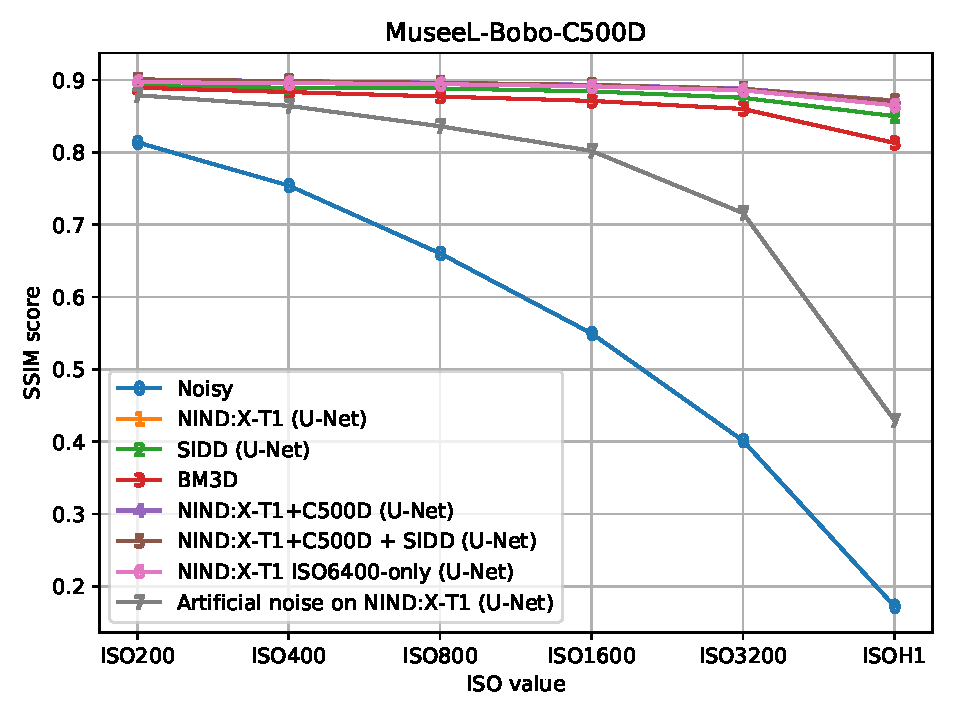
\includegraphics[width=1\linewidth]{gfx/graphs/boboc500d.pdf}
%%% Creator: Matplotlib, PGF backend
%%
%% To include the figure in your LaTeX document, write
%%   \input{<filename>.pgf}
%%
%% Make sure the required packages are loaded in your preamble
%%   \usepackage{pgf}
%%
%% Figures using additional raster images can only be included by \input if
%% they are in the same directory as the main LaTeX file. For loading figures
%% from other directories you can use the `import` package
%%   \usepackage{import}
%% and then include the figures with
%%   \import{<path to file>}{<filename>.pgf}
%%
%% Matplotlib used the following preamble
%%   \usepackage{fontspec}
%%   \setmainfont{DejaVuSerif.ttf}[Path=/usr/lib/python3.7/site-packages/matplotlib/mpl-data/fonts/ttf/]
%%   \setsansfont{DejaVuSans.ttf}[Path=/usr/lib/python3.7/site-packages/matplotlib/mpl-data/fonts/ttf/]
%%   \setmonofont{DejaVuSansMono.ttf}[Path=/usr/lib/python3.7/site-packages/matplotlib/mpl-data/fonts/ttf/]
%%
\begingroup%
\makeatletter%
\begin{pgfpicture}%
\pgfpathrectangle{\pgfpointorigin}{\pgfqpoint{38.400000in}{20.430000in}}%
\pgfusepath{use as bounding box, clip}%
\begin{pgfscope}%
\pgfsetbuttcap%
\pgfsetmiterjoin%
\definecolor{currentfill}{rgb}{1.000000,1.000000,1.000000}%
\pgfsetfillcolor{currentfill}%
\pgfsetlinewidth{0.000000pt}%
\definecolor{currentstroke}{rgb}{1.000000,1.000000,1.000000}%
\pgfsetstrokecolor{currentstroke}%
\pgfsetdash{}{0pt}%
\pgfpathmoveto{\pgfqpoint{0.000000in}{0.000000in}}%
\pgfpathlineto{\pgfqpoint{38.400000in}{0.000000in}}%
\pgfpathlineto{\pgfqpoint{38.400000in}{20.430000in}}%
\pgfpathlineto{\pgfqpoint{0.000000in}{20.430000in}}%
\pgfpathclose%
\pgfusepath{fill}%
\end{pgfscope}%
\begin{pgfscope}%
\pgfsetbuttcap%
\pgfsetmiterjoin%
\definecolor{currentfill}{rgb}{1.000000,1.000000,1.000000}%
\pgfsetfillcolor{currentfill}%
\pgfsetlinewidth{0.000000pt}%
\definecolor{currentstroke}{rgb}{0.000000,0.000000,0.000000}%
\pgfsetstrokecolor{currentstroke}%
\pgfsetstrokeopacity{0.000000}%
\pgfsetdash{}{0pt}%
\pgfpathmoveto{\pgfqpoint{0.662778in}{0.582778in}}%
\pgfpathlineto{\pgfqpoint{38.215000in}{0.582778in}}%
\pgfpathlineto{\pgfqpoint{38.215000in}{20.076667in}}%
\pgfpathlineto{\pgfqpoint{0.662778in}{20.076667in}}%
\pgfpathclose%
\pgfusepath{fill}%
\end{pgfscope}%
\begin{pgfscope}%
\pgfpathrectangle{\pgfqpoint{0.662778in}{0.582778in}}{\pgfqpoint{37.552222in}{19.493889in}}%
\pgfusepath{clip}%
\pgfsetrectcap%
\pgfsetroundjoin%
\pgfsetlinewidth{0.803000pt}%
\definecolor{currentstroke}{rgb}{0.690196,0.690196,0.690196}%
\pgfsetstrokecolor{currentstroke}%
\pgfsetdash{}{0pt}%
\pgfpathmoveto{\pgfqpoint{2.369697in}{0.582778in}}%
\pgfpathlineto{\pgfqpoint{2.369697in}{20.076667in}}%
\pgfusepath{stroke}%
\end{pgfscope}%
\begin{pgfscope}%
\pgfsetbuttcap%
\pgfsetroundjoin%
\definecolor{currentfill}{rgb}{0.000000,0.000000,0.000000}%
\pgfsetfillcolor{currentfill}%
\pgfsetlinewidth{0.803000pt}%
\definecolor{currentstroke}{rgb}{0.000000,0.000000,0.000000}%
\pgfsetstrokecolor{currentstroke}%
\pgfsetdash{}{0pt}%
\pgfsys@defobject{currentmarker}{\pgfqpoint{0.000000in}{-0.048611in}}{\pgfqpoint{0.000000in}{0.000000in}}{%
\pgfpathmoveto{\pgfqpoint{0.000000in}{0.000000in}}%
\pgfpathlineto{\pgfqpoint{0.000000in}{-0.048611in}}%
\pgfusepath{stroke,fill}%
}%
\begin{pgfscope}%
\pgfsys@transformshift{2.369697in}{0.582778in}%
\pgfsys@useobject{currentmarker}{}%
\end{pgfscope}%
\end{pgfscope}%
\begin{pgfscope}%
\definecolor{textcolor}{rgb}{0.000000,0.000000,0.000000}%
\pgfsetstrokecolor{textcolor}%
\pgfsetfillcolor{textcolor}%
\pgftext[x=2.369697in,y=0.485556in,,top]{\color{textcolor}\sffamily\fontsize{10.000000}{12.000000}\selectfont ISO200}%
\end{pgfscope}%
\begin{pgfscope}%
\pgfpathrectangle{\pgfqpoint{0.662778in}{0.582778in}}{\pgfqpoint{37.552222in}{19.493889in}}%
\pgfusepath{clip}%
\pgfsetrectcap%
\pgfsetroundjoin%
\pgfsetlinewidth{0.803000pt}%
\definecolor{currentstroke}{rgb}{0.690196,0.690196,0.690196}%
\pgfsetstrokecolor{currentstroke}%
\pgfsetdash{}{0pt}%
\pgfpathmoveto{\pgfqpoint{9.197374in}{0.582778in}}%
\pgfpathlineto{\pgfqpoint{9.197374in}{20.076667in}}%
\pgfusepath{stroke}%
\end{pgfscope}%
\begin{pgfscope}%
\pgfsetbuttcap%
\pgfsetroundjoin%
\definecolor{currentfill}{rgb}{0.000000,0.000000,0.000000}%
\pgfsetfillcolor{currentfill}%
\pgfsetlinewidth{0.803000pt}%
\definecolor{currentstroke}{rgb}{0.000000,0.000000,0.000000}%
\pgfsetstrokecolor{currentstroke}%
\pgfsetdash{}{0pt}%
\pgfsys@defobject{currentmarker}{\pgfqpoint{0.000000in}{-0.048611in}}{\pgfqpoint{0.000000in}{0.000000in}}{%
\pgfpathmoveto{\pgfqpoint{0.000000in}{0.000000in}}%
\pgfpathlineto{\pgfqpoint{0.000000in}{-0.048611in}}%
\pgfusepath{stroke,fill}%
}%
\begin{pgfscope}%
\pgfsys@transformshift{9.197374in}{0.582778in}%
\pgfsys@useobject{currentmarker}{}%
\end{pgfscope}%
\end{pgfscope}%
\begin{pgfscope}%
\definecolor{textcolor}{rgb}{0.000000,0.000000,0.000000}%
\pgfsetstrokecolor{textcolor}%
\pgfsetfillcolor{textcolor}%
\pgftext[x=9.197374in,y=0.485556in,,top]{\color{textcolor}\sffamily\fontsize{10.000000}{12.000000}\selectfont ISO400}%
\end{pgfscope}%
\begin{pgfscope}%
\pgfpathrectangle{\pgfqpoint{0.662778in}{0.582778in}}{\pgfqpoint{37.552222in}{19.493889in}}%
\pgfusepath{clip}%
\pgfsetrectcap%
\pgfsetroundjoin%
\pgfsetlinewidth{0.803000pt}%
\definecolor{currentstroke}{rgb}{0.690196,0.690196,0.690196}%
\pgfsetstrokecolor{currentstroke}%
\pgfsetdash{}{0pt}%
\pgfpathmoveto{\pgfqpoint{16.025051in}{0.582778in}}%
\pgfpathlineto{\pgfqpoint{16.025051in}{20.076667in}}%
\pgfusepath{stroke}%
\end{pgfscope}%
\begin{pgfscope}%
\pgfsetbuttcap%
\pgfsetroundjoin%
\definecolor{currentfill}{rgb}{0.000000,0.000000,0.000000}%
\pgfsetfillcolor{currentfill}%
\pgfsetlinewidth{0.803000pt}%
\definecolor{currentstroke}{rgb}{0.000000,0.000000,0.000000}%
\pgfsetstrokecolor{currentstroke}%
\pgfsetdash{}{0pt}%
\pgfsys@defobject{currentmarker}{\pgfqpoint{0.000000in}{-0.048611in}}{\pgfqpoint{0.000000in}{0.000000in}}{%
\pgfpathmoveto{\pgfqpoint{0.000000in}{0.000000in}}%
\pgfpathlineto{\pgfqpoint{0.000000in}{-0.048611in}}%
\pgfusepath{stroke,fill}%
}%
\begin{pgfscope}%
\pgfsys@transformshift{16.025051in}{0.582778in}%
\pgfsys@useobject{currentmarker}{}%
\end{pgfscope}%
\end{pgfscope}%
\begin{pgfscope}%
\definecolor{textcolor}{rgb}{0.000000,0.000000,0.000000}%
\pgfsetstrokecolor{textcolor}%
\pgfsetfillcolor{textcolor}%
\pgftext[x=16.025051in,y=0.485556in,,top]{\color{textcolor}\sffamily\fontsize{10.000000}{12.000000}\selectfont ISO800}%
\end{pgfscope}%
\begin{pgfscope}%
\pgfpathrectangle{\pgfqpoint{0.662778in}{0.582778in}}{\pgfqpoint{37.552222in}{19.493889in}}%
\pgfusepath{clip}%
\pgfsetrectcap%
\pgfsetroundjoin%
\pgfsetlinewidth{0.803000pt}%
\definecolor{currentstroke}{rgb}{0.690196,0.690196,0.690196}%
\pgfsetstrokecolor{currentstroke}%
\pgfsetdash{}{0pt}%
\pgfpathmoveto{\pgfqpoint{22.852727in}{0.582778in}}%
\pgfpathlineto{\pgfqpoint{22.852727in}{20.076667in}}%
\pgfusepath{stroke}%
\end{pgfscope}%
\begin{pgfscope}%
\pgfsetbuttcap%
\pgfsetroundjoin%
\definecolor{currentfill}{rgb}{0.000000,0.000000,0.000000}%
\pgfsetfillcolor{currentfill}%
\pgfsetlinewidth{0.803000pt}%
\definecolor{currentstroke}{rgb}{0.000000,0.000000,0.000000}%
\pgfsetstrokecolor{currentstroke}%
\pgfsetdash{}{0pt}%
\pgfsys@defobject{currentmarker}{\pgfqpoint{0.000000in}{-0.048611in}}{\pgfqpoint{0.000000in}{0.000000in}}{%
\pgfpathmoveto{\pgfqpoint{0.000000in}{0.000000in}}%
\pgfpathlineto{\pgfqpoint{0.000000in}{-0.048611in}}%
\pgfusepath{stroke,fill}%
}%
\begin{pgfscope}%
\pgfsys@transformshift{22.852727in}{0.582778in}%
\pgfsys@useobject{currentmarker}{}%
\end{pgfscope}%
\end{pgfscope}%
\begin{pgfscope}%
\definecolor{textcolor}{rgb}{0.000000,0.000000,0.000000}%
\pgfsetstrokecolor{textcolor}%
\pgfsetfillcolor{textcolor}%
\pgftext[x=22.852727in,y=0.485556in,,top]{\color{textcolor}\sffamily\fontsize{10.000000}{12.000000}\selectfont ISO1600}%
\end{pgfscope}%
\begin{pgfscope}%
\pgfpathrectangle{\pgfqpoint{0.662778in}{0.582778in}}{\pgfqpoint{37.552222in}{19.493889in}}%
\pgfusepath{clip}%
\pgfsetrectcap%
\pgfsetroundjoin%
\pgfsetlinewidth{0.803000pt}%
\definecolor{currentstroke}{rgb}{0.690196,0.690196,0.690196}%
\pgfsetstrokecolor{currentstroke}%
\pgfsetdash{}{0pt}%
\pgfpathmoveto{\pgfqpoint{29.680404in}{0.582778in}}%
\pgfpathlineto{\pgfqpoint{29.680404in}{20.076667in}}%
\pgfusepath{stroke}%
\end{pgfscope}%
\begin{pgfscope}%
\pgfsetbuttcap%
\pgfsetroundjoin%
\definecolor{currentfill}{rgb}{0.000000,0.000000,0.000000}%
\pgfsetfillcolor{currentfill}%
\pgfsetlinewidth{0.803000pt}%
\definecolor{currentstroke}{rgb}{0.000000,0.000000,0.000000}%
\pgfsetstrokecolor{currentstroke}%
\pgfsetdash{}{0pt}%
\pgfsys@defobject{currentmarker}{\pgfqpoint{0.000000in}{-0.048611in}}{\pgfqpoint{0.000000in}{0.000000in}}{%
\pgfpathmoveto{\pgfqpoint{0.000000in}{0.000000in}}%
\pgfpathlineto{\pgfqpoint{0.000000in}{-0.048611in}}%
\pgfusepath{stroke,fill}%
}%
\begin{pgfscope}%
\pgfsys@transformshift{29.680404in}{0.582778in}%
\pgfsys@useobject{currentmarker}{}%
\end{pgfscope}%
\end{pgfscope}%
\begin{pgfscope}%
\definecolor{textcolor}{rgb}{0.000000,0.000000,0.000000}%
\pgfsetstrokecolor{textcolor}%
\pgfsetfillcolor{textcolor}%
\pgftext[x=29.680404in,y=0.485556in,,top]{\color{textcolor}\sffamily\fontsize{10.000000}{12.000000}\selectfont ISO3200}%
\end{pgfscope}%
\begin{pgfscope}%
\pgfpathrectangle{\pgfqpoint{0.662778in}{0.582778in}}{\pgfqpoint{37.552222in}{19.493889in}}%
\pgfusepath{clip}%
\pgfsetrectcap%
\pgfsetroundjoin%
\pgfsetlinewidth{0.803000pt}%
\definecolor{currentstroke}{rgb}{0.690196,0.690196,0.690196}%
\pgfsetstrokecolor{currentstroke}%
\pgfsetdash{}{0pt}%
\pgfpathmoveto{\pgfqpoint{36.508081in}{0.582778in}}%
\pgfpathlineto{\pgfqpoint{36.508081in}{20.076667in}}%
\pgfusepath{stroke}%
\end{pgfscope}%
\begin{pgfscope}%
\pgfsetbuttcap%
\pgfsetroundjoin%
\definecolor{currentfill}{rgb}{0.000000,0.000000,0.000000}%
\pgfsetfillcolor{currentfill}%
\pgfsetlinewidth{0.803000pt}%
\definecolor{currentstroke}{rgb}{0.000000,0.000000,0.000000}%
\pgfsetstrokecolor{currentstroke}%
\pgfsetdash{}{0pt}%
\pgfsys@defobject{currentmarker}{\pgfqpoint{0.000000in}{-0.048611in}}{\pgfqpoint{0.000000in}{0.000000in}}{%
\pgfpathmoveto{\pgfqpoint{0.000000in}{0.000000in}}%
\pgfpathlineto{\pgfqpoint{0.000000in}{-0.048611in}}%
\pgfusepath{stroke,fill}%
}%
\begin{pgfscope}%
\pgfsys@transformshift{36.508081in}{0.582778in}%
\pgfsys@useobject{currentmarker}{}%
\end{pgfscope}%
\end{pgfscope}%
\begin{pgfscope}%
\definecolor{textcolor}{rgb}{0.000000,0.000000,0.000000}%
\pgfsetstrokecolor{textcolor}%
\pgfsetfillcolor{textcolor}%
\pgftext[x=36.508081in,y=0.485556in,,top]{\color{textcolor}\sffamily\fontsize{10.000000}{12.000000}\selectfont ISOH1}%
\end{pgfscope}%
\begin{pgfscope}%
\definecolor{textcolor}{rgb}{0.000000,0.000000,0.000000}%
\pgfsetstrokecolor{textcolor}%
\pgfsetfillcolor{textcolor}%
\pgftext[x=19.438889in,y=0.295587in,,top]{\color{textcolor}\sffamily\fontsize{10.000000}{12.000000}\selectfont ISO value}%
\end{pgfscope}%
\begin{pgfscope}%
\pgfpathrectangle{\pgfqpoint{0.662778in}{0.582778in}}{\pgfqpoint{37.552222in}{19.493889in}}%
\pgfusepath{clip}%
\pgfsetrectcap%
\pgfsetroundjoin%
\pgfsetlinewidth{0.803000pt}%
\definecolor{currentstroke}{rgb}{0.690196,0.690196,0.690196}%
\pgfsetstrokecolor{currentstroke}%
\pgfsetdash{}{0pt}%
\pgfpathmoveto{\pgfqpoint{0.662778in}{8.491192in}}%
\pgfpathlineto{\pgfqpoint{38.215000in}{8.491192in}}%
\pgfusepath{stroke}%
\end{pgfscope}%
\begin{pgfscope}%
\pgfsetbuttcap%
\pgfsetroundjoin%
\definecolor{currentfill}{rgb}{0.000000,0.000000,0.000000}%
\pgfsetfillcolor{currentfill}%
\pgfsetlinewidth{0.803000pt}%
\definecolor{currentstroke}{rgb}{0.000000,0.000000,0.000000}%
\pgfsetstrokecolor{currentstroke}%
\pgfsetdash{}{0pt}%
\pgfsys@defobject{currentmarker}{\pgfqpoint{-0.048611in}{0.000000in}}{\pgfqpoint{0.000000in}{0.000000in}}{%
\pgfpathmoveto{\pgfqpoint{0.000000in}{0.000000in}}%
\pgfpathlineto{\pgfqpoint{-0.048611in}{0.000000in}}%
\pgfusepath{stroke,fill}%
}%
\begin{pgfscope}%
\pgfsys@transformshift{0.662778in}{8.491192in}%
\pgfsys@useobject{currentmarker}{}%
\end{pgfscope}%
\end{pgfscope}%
\begin{pgfscope}%
\definecolor{textcolor}{rgb}{0.000000,0.000000,0.000000}%
\pgfsetstrokecolor{textcolor}%
\pgfsetfillcolor{textcolor}%
\pgftext[x=0.256311in,y=8.438430in,left,base]{\color{textcolor}\sffamily\fontsize{10.000000}{12.000000}\selectfont 0.50}%
\end{pgfscope}%
\begin{pgfscope}%
\pgfpathrectangle{\pgfqpoint{0.662778in}{0.582778in}}{\pgfqpoint{37.552222in}{19.493889in}}%
\pgfusepath{clip}%
\pgfsetrectcap%
\pgfsetroundjoin%
\pgfsetlinewidth{0.803000pt}%
\definecolor{currentstroke}{rgb}{0.690196,0.690196,0.690196}%
\pgfsetstrokecolor{currentstroke}%
\pgfsetdash{}{0pt}%
\pgfpathmoveto{\pgfqpoint{0.662778in}{17.887141in}}%
\pgfpathlineto{\pgfqpoint{38.215000in}{17.887141in}}%
\pgfusepath{stroke}%
\end{pgfscope}%
\begin{pgfscope}%
\pgfsetbuttcap%
\pgfsetroundjoin%
\definecolor{currentfill}{rgb}{0.000000,0.000000,0.000000}%
\pgfsetfillcolor{currentfill}%
\pgfsetlinewidth{0.803000pt}%
\definecolor{currentstroke}{rgb}{0.000000,0.000000,0.000000}%
\pgfsetstrokecolor{currentstroke}%
\pgfsetdash{}{0pt}%
\pgfsys@defobject{currentmarker}{\pgfqpoint{-0.048611in}{0.000000in}}{\pgfqpoint{0.000000in}{0.000000in}}{%
\pgfpathmoveto{\pgfqpoint{0.000000in}{0.000000in}}%
\pgfpathlineto{\pgfqpoint{-0.048611in}{0.000000in}}%
\pgfusepath{stroke,fill}%
}%
\begin{pgfscope}%
\pgfsys@transformshift{0.662778in}{17.887141in}%
\pgfsys@useobject{currentmarker}{}%
\end{pgfscope}%
\end{pgfscope}%
\begin{pgfscope}%
\definecolor{textcolor}{rgb}{0.000000,0.000000,0.000000}%
\pgfsetstrokecolor{textcolor}%
\pgfsetfillcolor{textcolor}%
\pgftext[x=0.256311in,y=17.834379in,left,base]{\color{textcolor}\sffamily\fontsize{10.000000}{12.000000}\selectfont 0.90}%
\end{pgfscope}%
\begin{pgfscope}%
\pgfsetbuttcap%
\pgfsetroundjoin%
\definecolor{currentfill}{rgb}{0.000000,0.000000,0.000000}%
\pgfsetfillcolor{currentfill}%
\pgfsetlinewidth{0.602250pt}%
\definecolor{currentstroke}{rgb}{0.000000,0.000000,0.000000}%
\pgfsetstrokecolor{currentstroke}%
\pgfsetdash{}{0pt}%
\pgfsys@defobject{currentmarker}{\pgfqpoint{-0.027778in}{0.000000in}}{\pgfqpoint{0.000000in}{0.000000in}}{%
\pgfpathmoveto{\pgfqpoint{0.000000in}{0.000000in}}%
\pgfpathlineto{\pgfqpoint{-0.027778in}{0.000000in}}%
\pgfusepath{stroke,fill}%
}%
\begin{pgfscope}%
\pgfsys@transformshift{0.662778in}{2.563008in}%
\pgfsys@useobject{currentmarker}{}%
\end{pgfscope}%
\end{pgfscope}%
\begin{pgfscope}%
\definecolor{textcolor}{rgb}{0.000000,0.000000,0.000000}%
\pgfsetstrokecolor{textcolor}%
\pgfsetfillcolor{textcolor}%
\pgftext[x=0.278533in,y=2.510247in,left,base]{\color{textcolor}\sffamily\fontsize{10.000000}{12.000000}\selectfont 0.20}%
\end{pgfscope}%
\begin{pgfscope}%
\pgfsetbuttcap%
\pgfsetroundjoin%
\definecolor{currentfill}{rgb}{0.000000,0.000000,0.000000}%
\pgfsetfillcolor{currentfill}%
\pgfsetlinewidth{0.602250pt}%
\definecolor{currentstroke}{rgb}{0.000000,0.000000,0.000000}%
\pgfsetstrokecolor{currentstroke}%
\pgfsetdash{}{0pt}%
\pgfsys@defobject{currentmarker}{\pgfqpoint{-0.027778in}{0.000000in}}{\pgfqpoint{0.000000in}{0.000000in}}{%
\pgfpathmoveto{\pgfqpoint{0.000000in}{0.000000in}}%
\pgfpathlineto{\pgfqpoint{-0.027778in}{0.000000in}}%
\pgfusepath{stroke,fill}%
}%
\begin{pgfscope}%
\pgfsys@transformshift{0.662778in}{4.867908in}%
\pgfsys@useobject{currentmarker}{}%
\end{pgfscope}%
\end{pgfscope}%
\begin{pgfscope}%
\definecolor{textcolor}{rgb}{0.000000,0.000000,0.000000}%
\pgfsetstrokecolor{textcolor}%
\pgfsetfillcolor{textcolor}%
\pgftext[x=0.278533in,y=4.815147in,left,base]{\color{textcolor}\sffamily\fontsize{10.000000}{12.000000}\selectfont 0.30}%
\end{pgfscope}%
\begin{pgfscope}%
\pgfsetbuttcap%
\pgfsetroundjoin%
\definecolor{currentfill}{rgb}{0.000000,0.000000,0.000000}%
\pgfsetfillcolor{currentfill}%
\pgfsetlinewidth{0.602250pt}%
\definecolor{currentstroke}{rgb}{0.000000,0.000000,0.000000}%
\pgfsetstrokecolor{currentstroke}%
\pgfsetdash{}{0pt}%
\pgfsys@defobject{currentmarker}{\pgfqpoint{-0.027778in}{0.000000in}}{\pgfqpoint{0.000000in}{0.000000in}}{%
\pgfpathmoveto{\pgfqpoint{0.000000in}{0.000000in}}%
\pgfpathlineto{\pgfqpoint{-0.027778in}{0.000000in}}%
\pgfusepath{stroke,fill}%
}%
\begin{pgfscope}%
\pgfsys@transformshift{0.662778in}{6.757309in}%
\pgfsys@useobject{currentmarker}{}%
\end{pgfscope}%
\end{pgfscope}%
\begin{pgfscope}%
\definecolor{textcolor}{rgb}{0.000000,0.000000,0.000000}%
\pgfsetstrokecolor{textcolor}%
\pgfsetfillcolor{textcolor}%
\pgftext[x=0.278533in,y=6.704548in,left,base]{\color{textcolor}\sffamily\fontsize{10.000000}{12.000000}\selectfont 0.40}%
\end{pgfscope}%
\begin{pgfscope}%
\pgfsetbuttcap%
\pgfsetroundjoin%
\definecolor{currentfill}{rgb}{0.000000,0.000000,0.000000}%
\pgfsetfillcolor{currentfill}%
\pgfsetlinewidth{0.602250pt}%
\definecolor{currentstroke}{rgb}{0.000000,0.000000,0.000000}%
\pgfsetstrokecolor{currentstroke}%
\pgfsetdash{}{0pt}%
\pgfsys@defobject{currentmarker}{\pgfqpoint{-0.027778in}{0.000000in}}{\pgfqpoint{0.000000in}{0.000000in}}{%
\pgfpathmoveto{\pgfqpoint{0.000000in}{0.000000in}}%
\pgfpathlineto{\pgfqpoint{-0.027778in}{0.000000in}}%
\pgfusepath{stroke,fill}%
}%
\begin{pgfscope}%
\pgfsys@transformshift{0.662778in}{10.225075in}%
\pgfsys@useobject{currentmarker}{}%
\end{pgfscope}%
\end{pgfscope}%
\begin{pgfscope}%
\definecolor{textcolor}{rgb}{0.000000,0.000000,0.000000}%
\pgfsetstrokecolor{textcolor}%
\pgfsetfillcolor{textcolor}%
\pgftext[x=0.278533in,y=10.172313in,left,base]{\color{textcolor}\sffamily\fontsize{10.000000}{12.000000}\selectfont 0.60}%
\end{pgfscope}%
\begin{pgfscope}%
\pgfsetbuttcap%
\pgfsetroundjoin%
\definecolor{currentfill}{rgb}{0.000000,0.000000,0.000000}%
\pgfsetfillcolor{currentfill}%
\pgfsetlinewidth{0.602250pt}%
\definecolor{currentstroke}{rgb}{0.000000,0.000000,0.000000}%
\pgfsetstrokecolor{currentstroke}%
\pgfsetdash{}{0pt}%
\pgfsys@defobject{currentmarker}{\pgfqpoint{-0.027778in}{0.000000in}}{\pgfqpoint{0.000000in}{0.000000in}}{%
\pgfpathmoveto{\pgfqpoint{0.000000in}{0.000000in}}%
\pgfpathlineto{\pgfqpoint{-0.027778in}{0.000000in}}%
\pgfusepath{stroke,fill}%
}%
\begin{pgfscope}%
\pgfsys@transformshift{0.662778in}{12.114475in}%
\pgfsys@useobject{currentmarker}{}%
\end{pgfscope}%
\end{pgfscope}%
\begin{pgfscope}%
\definecolor{textcolor}{rgb}{0.000000,0.000000,0.000000}%
\pgfsetstrokecolor{textcolor}%
\pgfsetfillcolor{textcolor}%
\pgftext[x=0.278533in,y=12.061714in,left,base]{\color{textcolor}\sffamily\fontsize{10.000000}{12.000000}\selectfont 0.70}%
\end{pgfscope}%
\begin{pgfscope}%
\pgfsetbuttcap%
\pgfsetroundjoin%
\definecolor{currentfill}{rgb}{0.000000,0.000000,0.000000}%
\pgfsetfillcolor{currentfill}%
\pgfsetlinewidth{0.602250pt}%
\definecolor{currentstroke}{rgb}{0.000000,0.000000,0.000000}%
\pgfsetstrokecolor{currentstroke}%
\pgfsetdash{}{0pt}%
\pgfsys@defobject{currentmarker}{\pgfqpoint{-0.027778in}{0.000000in}}{\pgfqpoint{0.000000in}{0.000000in}}{%
\pgfpathmoveto{\pgfqpoint{0.000000in}{0.000000in}}%
\pgfpathlineto{\pgfqpoint{-0.027778in}{0.000000in}}%
\pgfusepath{stroke,fill}%
}%
\begin{pgfscope}%
\pgfsys@transformshift{0.662778in}{14.419376in}%
\pgfsys@useobject{currentmarker}{}%
\end{pgfscope}%
\end{pgfscope}%
\begin{pgfscope}%
\definecolor{textcolor}{rgb}{0.000000,0.000000,0.000000}%
\pgfsetstrokecolor{textcolor}%
\pgfsetfillcolor{textcolor}%
\pgftext[x=0.278533in,y=14.366614in,left,base]{\color{textcolor}\sffamily\fontsize{10.000000}{12.000000}\selectfont 0.80}%
\end{pgfscope}%
\begin{pgfscope}%
\pgfsetbuttcap%
\pgfsetroundjoin%
\definecolor{currentfill}{rgb}{0.000000,0.000000,0.000000}%
\pgfsetfillcolor{currentfill}%
\pgfsetlinewidth{0.602250pt}%
\definecolor{currentstroke}{rgb}{0.000000,0.000000,0.000000}%
\pgfsetstrokecolor{currentstroke}%
\pgfsetdash{}{0pt}%
\pgfsys@defobject{currentmarker}{\pgfqpoint{-0.027778in}{0.000000in}}{\pgfqpoint{0.000000in}{0.000000in}}{%
\pgfpathmoveto{\pgfqpoint{0.000000in}{0.000000in}}%
\pgfpathlineto{\pgfqpoint{-0.027778in}{0.000000in}}%
\pgfusepath{stroke,fill}%
}%
\begin{pgfscope}%
\pgfsys@transformshift{0.662778in}{19.552602in}%
\pgfsys@useobject{currentmarker}{}%
\end{pgfscope}%
\end{pgfscope}%
\begin{pgfscope}%
\definecolor{textcolor}{rgb}{0.000000,0.000000,0.000000}%
\pgfsetstrokecolor{textcolor}%
\pgfsetfillcolor{textcolor}%
\pgftext[x=0.278533in,y=19.499840in,left,base]{\color{textcolor}\sffamily\fontsize{10.000000}{12.000000}\selectfont 0.93}%
\end{pgfscope}%
\begin{pgfscope}%
\pgfsetbuttcap%
\pgfsetroundjoin%
\definecolor{currentfill}{rgb}{0.000000,0.000000,0.000000}%
\pgfsetfillcolor{currentfill}%
\pgfsetlinewidth{0.602250pt}%
\definecolor{currentstroke}{rgb}{0.000000,0.000000,0.000000}%
\pgfsetstrokecolor{currentstroke}%
\pgfsetdash{}{0pt}%
\pgfsys@defobject{currentmarker}{\pgfqpoint{-0.027778in}{0.000000in}}{\pgfqpoint{0.000000in}{0.000000in}}{%
\pgfpathmoveto{\pgfqpoint{0.000000in}{0.000000in}}%
\pgfpathlineto{\pgfqpoint{-0.027778in}{0.000000in}}%
\pgfusepath{stroke,fill}%
}%
\begin{pgfscope}%
\pgfsys@transformshift{0.662778in}{18.935353in}%
\pgfsys@useobject{currentmarker}{}%
\end{pgfscope}%
\end{pgfscope}%
\begin{pgfscope}%
\definecolor{textcolor}{rgb}{0.000000,0.000000,0.000000}%
\pgfsetstrokecolor{textcolor}%
\pgfsetfillcolor{textcolor}%
\pgftext[x=0.278533in,y=18.882592in,left,base]{\color{textcolor}\sffamily\fontsize{10.000000}{12.000000}\selectfont 0.92}%
\end{pgfscope}%
\begin{pgfscope}%
\pgfsetbuttcap%
\pgfsetroundjoin%
\definecolor{currentfill}{rgb}{0.000000,0.000000,0.000000}%
\pgfsetfillcolor{currentfill}%
\pgfsetlinewidth{0.602250pt}%
\definecolor{currentstroke}{rgb}{0.000000,0.000000,0.000000}%
\pgfsetstrokecolor{currentstroke}%
\pgfsetdash{}{0pt}%
\pgfsys@defobject{currentmarker}{\pgfqpoint{-0.027778in}{0.000000in}}{\pgfqpoint{0.000000in}{0.000000in}}{%
\pgfpathmoveto{\pgfqpoint{0.000000in}{0.000000in}}%
\pgfpathlineto{\pgfqpoint{-0.027778in}{0.000000in}}%
\pgfusepath{stroke,fill}%
}%
\begin{pgfscope}%
\pgfsys@transformshift{0.662778in}{18.384944in}%
\pgfsys@useobject{currentmarker}{}%
\end{pgfscope}%
\end{pgfscope}%
\begin{pgfscope}%
\definecolor{textcolor}{rgb}{0.000000,0.000000,0.000000}%
\pgfsetstrokecolor{textcolor}%
\pgfsetfillcolor{textcolor}%
\pgftext[x=0.278533in,y=18.332183in,left,base]{\color{textcolor}\sffamily\fontsize{10.000000}{12.000000}\selectfont 0.91}%
\end{pgfscope}%
\begin{pgfscope}%
\definecolor{textcolor}{rgb}{0.000000,0.000000,0.000000}%
\pgfsetstrokecolor{textcolor}%
\pgfsetfillcolor{textcolor}%
\pgftext[x=0.200755in,y=10.329722in,,bottom,rotate=90.000000]{\color{textcolor}\sffamily\fontsize{10.000000}{12.000000}\selectfont SSIM score}%
\end{pgfscope}%
\begin{pgfscope}%
\pgfpathrectangle{\pgfqpoint{0.662778in}{0.582778in}}{\pgfqpoint{37.552222in}{19.493889in}}%
\pgfusepath{clip}%
\pgfsetrectcap%
\pgfsetroundjoin%
\pgfsetlinewidth{1.505625pt}%
\definecolor{currentstroke}{rgb}{0.121569,0.466667,0.705882}%
\pgfsetstrokecolor{currentstroke}%
\pgfsetdash{}{0pt}%
\pgfpathmoveto{\pgfqpoint{2.369697in}{14.802371in}}%
\pgfpathlineto{\pgfqpoint{9.197374in}{13.286628in}}%
\pgfpathlineto{\pgfqpoint{16.025051in}{11.334506in}}%
\pgfpathlineto{\pgfqpoint{22.852727in}{9.344757in}}%
\pgfpathlineto{\pgfqpoint{29.680404in}{6.781277in}}%
\pgfpathlineto{\pgfqpoint{36.508081in}{1.782474in}}%
\pgfusepath{stroke}%
\end{pgfscope}%
\begin{pgfscope}%
\pgfpathrectangle{\pgfqpoint{0.662778in}{0.582778in}}{\pgfqpoint{37.552222in}{19.493889in}}%
\pgfusepath{clip}%
\pgfsetbuttcap%
\pgfsetroundjoin%
\definecolor{currentfill}{rgb}{0.121569,0.466667,0.705882}%
\pgfsetfillcolor{currentfill}%
\pgfsetlinewidth{1.003750pt}%
\definecolor{currentstroke}{rgb}{0.121569,0.466667,0.705882}%
\pgfsetstrokecolor{currentstroke}%
\pgfsetdash{}{0pt}%
\pgfsys@defobject{currentmarker}{\pgfqpoint{-0.024126in}{-0.041667in}}{\pgfqpoint{0.031390in}{0.041667in}}{%
\pgfpathmoveto{\pgfqpoint{0.003624in}{0.033060in}}%
\pgfpathquadraticcurveto{\pgfqpoint{-0.004760in}{0.033060in}}{\pgfqpoint{-0.008994in}{0.024797in}}%
\pgfpathquadraticcurveto{\pgfqpoint{-0.013212in}{0.016551in}}{\pgfqpoint{-0.013212in}{-0.000026in}}%
\pgfpathquadraticcurveto{\pgfqpoint{-0.013212in}{-0.016534in}}{\pgfqpoint{-0.008994in}{-0.024797in}}%
\pgfpathquadraticcurveto{\pgfqpoint{-0.004760in}{-0.033060in}}{\pgfqpoint{0.003624in}{-0.033060in}}%
\pgfpathquadraticcurveto{\pgfqpoint{0.012076in}{-0.033060in}}{\pgfqpoint{0.016293in}{-0.024797in}}%
\pgfpathquadraticcurveto{\pgfqpoint{0.020528in}{-0.016534in}}{\pgfqpoint{0.020528in}{-0.000026in}}%
\pgfpathquadraticcurveto{\pgfqpoint{0.020528in}{0.016551in}}{\pgfqpoint{0.016293in}{0.024797in}}%
\pgfpathquadraticcurveto{\pgfqpoint{0.012076in}{0.033060in}}{\pgfqpoint{0.003624in}{0.033060in}}%
\pgfpathclose%
\pgfpathmoveto{\pgfqpoint{0.003624in}{0.041667in}}%
\pgfpathquadraticcurveto{\pgfqpoint{0.017137in}{0.041667in}}{\pgfqpoint{0.024263in}{0.030977in}}%
\pgfpathquadraticcurveto{\pgfqpoint{0.031390in}{0.020304in}}{\pgfqpoint{0.031390in}{-0.000026in}}%
\pgfpathquadraticcurveto{\pgfqpoint{0.031390in}{-0.020304in}}{\pgfqpoint{0.024263in}{-0.030994in}}%
\pgfpathquadraticcurveto{\pgfqpoint{0.017137in}{-0.041667in}}{\pgfqpoint{0.003624in}{-0.041667in}}%
\pgfpathquadraticcurveto{\pgfqpoint{-0.009872in}{-0.041667in}}{\pgfqpoint{-0.016999in}{-0.030994in}}%
\pgfpathquadraticcurveto{\pgfqpoint{-0.024126in}{-0.020304in}}{\pgfqpoint{-0.024126in}{-0.000026in}}%
\pgfpathquadraticcurveto{\pgfqpoint{-0.024126in}{0.020304in}}{\pgfqpoint{-0.016999in}{0.030977in}}%
\pgfpathquadraticcurveto{\pgfqpoint{-0.009872in}{0.041667in}}{\pgfqpoint{0.003624in}{0.041667in}}%
\pgfpathclose%
\pgfusepath{stroke,fill}%
}%
\begin{pgfscope}%
\pgfsys@transformshift{2.369697in}{14.802371in}%
\pgfsys@useobject{currentmarker}{}%
\end{pgfscope}%
\begin{pgfscope}%
\pgfsys@transformshift{9.197374in}{13.286628in}%
\pgfsys@useobject{currentmarker}{}%
\end{pgfscope}%
\begin{pgfscope}%
\pgfsys@transformshift{16.025051in}{11.334506in}%
\pgfsys@useobject{currentmarker}{}%
\end{pgfscope}%
\begin{pgfscope}%
\pgfsys@transformshift{22.852727in}{9.344757in}%
\pgfsys@useobject{currentmarker}{}%
\end{pgfscope}%
\begin{pgfscope}%
\pgfsys@transformshift{29.680404in}{6.781277in}%
\pgfsys@useobject{currentmarker}{}%
\end{pgfscope}%
\begin{pgfscope}%
\pgfsys@transformshift{36.508081in}{1.782474in}%
\pgfsys@useobject{currentmarker}{}%
\end{pgfscope}%
\end{pgfscope}%
\begin{pgfscope}%
\pgfpathrectangle{\pgfqpoint{0.662778in}{0.582778in}}{\pgfqpoint{37.552222in}{19.493889in}}%
\pgfusepath{clip}%
\pgfsetrectcap%
\pgfsetroundjoin%
\pgfsetlinewidth{1.505625pt}%
\definecolor{currentstroke}{rgb}{1.000000,0.498039,0.054902}%
\pgfsetstrokecolor{currentstroke}%
\pgfsetdash{}{0pt}%
\pgfpathmoveto{\pgfqpoint{2.369697in}{17.930816in}}%
\pgfpathlineto{\pgfqpoint{9.197374in}{17.802533in}}%
\pgfpathlineto{\pgfqpoint{16.025051in}{17.682881in}}%
\pgfpathlineto{\pgfqpoint{22.852727in}{17.543258in}}%
\pgfpathlineto{\pgfqpoint{29.680404in}{17.297215in}}%
\pgfpathlineto{\pgfqpoint{36.508081in}{16.547206in}}%
\pgfusepath{stroke}%
\end{pgfscope}%
\begin{pgfscope}%
\pgfpathrectangle{\pgfqpoint{0.662778in}{0.582778in}}{\pgfqpoint{37.552222in}{19.493889in}}%
\pgfusepath{clip}%
\pgfsetbuttcap%
\pgfsetroundjoin%
\definecolor{currentfill}{rgb}{1.000000,0.498039,0.054902}%
\pgfsetfillcolor{currentfill}%
\pgfsetlinewidth{1.003750pt}%
\definecolor{currentstroke}{rgb}{1.000000,0.498039,0.054902}%
\pgfsetstrokecolor{currentstroke}%
\pgfsetdash{}{0pt}%
\pgfsys@defobject{currentmarker}{\pgfqpoint{-0.018529in}{-0.041667in}}{\pgfqpoint{0.031085in}{0.041667in}}{%
\pgfpathmoveto{\pgfqpoint{-0.016904in}{-0.032183in}}%
\pgfpathlineto{\pgfqpoint{0.001509in}{-0.032183in}}%
\pgfpathlineto{\pgfqpoint{0.001509in}{0.031397in}}%
\pgfpathlineto{\pgfqpoint{-0.018529in}{0.027379in}}%
\pgfpathlineto{\pgfqpoint{-0.018529in}{0.037648in}}%
\pgfpathlineto{\pgfqpoint{0.001402in}{0.041667in}}%
\pgfpathlineto{\pgfqpoint{0.012671in}{0.041667in}}%
\pgfpathlineto{\pgfqpoint{0.012671in}{-0.032183in}}%
\pgfpathlineto{\pgfqpoint{0.031085in}{-0.032183in}}%
\pgfpathlineto{\pgfqpoint{0.031085in}{-0.041667in}}%
\pgfpathlineto{\pgfqpoint{-0.016904in}{-0.041667in}}%
\pgfpathclose%
\pgfusepath{stroke,fill}%
}%
\begin{pgfscope}%
\pgfsys@transformshift{2.369697in}{17.930816in}%
\pgfsys@useobject{currentmarker}{}%
\end{pgfscope}%
\begin{pgfscope}%
\pgfsys@transformshift{9.197374in}{17.802533in}%
\pgfsys@useobject{currentmarker}{}%
\end{pgfscope}%
\begin{pgfscope}%
\pgfsys@transformshift{16.025051in}{17.682881in}%
\pgfsys@useobject{currentmarker}{}%
\end{pgfscope}%
\begin{pgfscope}%
\pgfsys@transformshift{22.852727in}{17.543258in}%
\pgfsys@useobject{currentmarker}{}%
\end{pgfscope}%
\begin{pgfscope}%
\pgfsys@transformshift{29.680404in}{17.297215in}%
\pgfsys@useobject{currentmarker}{}%
\end{pgfscope}%
\begin{pgfscope}%
\pgfsys@transformshift{36.508081in}{16.547206in}%
\pgfsys@useobject{currentmarker}{}%
\end{pgfscope}%
\end{pgfscope}%
\begin{pgfscope}%
\pgfpathrectangle{\pgfqpoint{0.662778in}{0.582778in}}{\pgfqpoint{37.552222in}{19.493889in}}%
\pgfusepath{clip}%
\pgfsetrectcap%
\pgfsetroundjoin%
\pgfsetlinewidth{1.505625pt}%
\definecolor{currentstroke}{rgb}{0.172549,0.627451,0.172549}%
\pgfsetstrokecolor{currentstroke}%
\pgfsetdash{}{0pt}%
\pgfpathmoveto{\pgfqpoint{2.369697in}{17.511285in}}%
\pgfpathlineto{\pgfqpoint{9.197374in}{17.410174in}}%
\pgfpathlineto{\pgfqpoint{16.025051in}{17.369351in}}%
\pgfpathlineto{\pgfqpoint{22.852727in}{17.197518in}}%
\pgfpathlineto{\pgfqpoint{29.680404in}{16.837475in}}%
\pgfpathlineto{\pgfqpoint{36.508081in}{15.915330in}}%
\pgfusepath{stroke}%
\end{pgfscope}%
\begin{pgfscope}%
\pgfpathrectangle{\pgfqpoint{0.662778in}{0.582778in}}{\pgfqpoint{37.552222in}{19.493889in}}%
\pgfusepath{clip}%
\pgfsetbuttcap%
\pgfsetroundjoin%
\definecolor{currentfill}{rgb}{0.172549,0.627451,0.172549}%
\pgfsetfillcolor{currentfill}%
\pgfsetlinewidth{1.003750pt}%
\definecolor{currentstroke}{rgb}{0.172549,0.627451,0.172549}%
\pgfsetstrokecolor{currentstroke}%
\pgfsetdash{}{0pt}%
\pgfsys@defobject{currentmarker}{\pgfqpoint{-0.021868in}{-0.041667in}}{\pgfqpoint{0.030096in}{0.041667in}}{%
\pgfpathmoveto{\pgfqpoint{-0.008553in}{-0.032351in}}%
\pgfpathlineto{\pgfqpoint{0.030096in}{-0.032351in}}%
\pgfpathlineto{\pgfqpoint{0.030096in}{-0.041667in}}%
\pgfpathlineto{\pgfqpoint{-0.021868in}{-0.041667in}}%
\pgfpathlineto{\pgfqpoint{-0.021868in}{-0.032351in}}%
\pgfpathquadraticcurveto{\pgfqpoint{-0.015570in}{-0.025825in}}{\pgfqpoint{-0.004693in}{-0.014842in}}%
\pgfpathquadraticcurveto{\pgfqpoint{0.006202in}{-0.003842in}}{\pgfqpoint{0.008991in}{-0.000649in}}%
\pgfpathquadraticcurveto{\pgfqpoint{0.014307in}{0.005316in}}{\pgfqpoint{0.016412in}{0.009456in}}%
\pgfpathquadraticcurveto{\pgfqpoint{0.018535in}{0.013596in}}{\pgfqpoint{0.018535in}{0.017596in}}%
\pgfpathquadraticcurveto{\pgfqpoint{0.018535in}{0.024123in}}{\pgfqpoint{0.013956in}{0.028228in}}%
\pgfpathquadraticcurveto{\pgfqpoint{0.009377in}{0.032351in}}{\pgfqpoint{0.002026in}{0.032351in}}%
\pgfpathquadraticcurveto{\pgfqpoint{-0.003184in}{0.032351in}}{\pgfqpoint{-0.008974in}{0.030544in}}%
\pgfpathquadraticcurveto{\pgfqpoint{-0.014746in}{0.028737in}}{\pgfqpoint{-0.021325in}{0.025053in}}%
\pgfpathlineto{\pgfqpoint{-0.021325in}{0.036246in}}%
\pgfpathquadraticcurveto{\pgfqpoint{-0.014640in}{0.038930in}}{\pgfqpoint{-0.008833in}{0.040298in}}%
\pgfpathquadraticcurveto{\pgfqpoint{-0.003009in}{0.041667in}}{\pgfqpoint{0.001816in}{0.041667in}}%
\pgfpathquadraticcurveto{\pgfqpoint{0.014535in}{0.041667in}}{\pgfqpoint{0.022096in}{0.035298in}}%
\pgfpathquadraticcurveto{\pgfqpoint{0.029658in}{0.028947in}}{\pgfqpoint{0.029658in}{0.018316in}}%
\pgfpathquadraticcurveto{\pgfqpoint{0.029658in}{0.013263in}}{\pgfqpoint{0.027763in}{0.008737in}}%
\pgfpathquadraticcurveto{\pgfqpoint{0.025886in}{0.004228in}}{\pgfqpoint{0.020886in}{-0.001912in}}%
\pgfpathquadraticcurveto{\pgfqpoint{0.019518in}{-0.003509in}}{\pgfqpoint{0.012167in}{-0.011105in}}%
\pgfpathquadraticcurveto{\pgfqpoint{0.004833in}{-0.018702in}}{\pgfqpoint{-0.008553in}{-0.032351in}}%
\pgfpathclose%
\pgfusepath{stroke,fill}%
}%
\begin{pgfscope}%
\pgfsys@transformshift{2.369697in}{17.511285in}%
\pgfsys@useobject{currentmarker}{}%
\end{pgfscope}%
\begin{pgfscope}%
\pgfsys@transformshift{9.197374in}{17.410174in}%
\pgfsys@useobject{currentmarker}{}%
\end{pgfscope}%
\begin{pgfscope}%
\pgfsys@transformshift{16.025051in}{17.369351in}%
\pgfsys@useobject{currentmarker}{}%
\end{pgfscope}%
\begin{pgfscope}%
\pgfsys@transformshift{22.852727in}{17.197518in}%
\pgfsys@useobject{currentmarker}{}%
\end{pgfscope}%
\begin{pgfscope}%
\pgfsys@transformshift{29.680404in}{16.837475in}%
\pgfsys@useobject{currentmarker}{}%
\end{pgfscope}%
\begin{pgfscope}%
\pgfsys@transformshift{36.508081in}{15.915330in}%
\pgfsys@useobject{currentmarker}{}%
\end{pgfscope}%
\end{pgfscope}%
\begin{pgfscope}%
\pgfpathrectangle{\pgfqpoint{0.662778in}{0.582778in}}{\pgfqpoint{37.552222in}{19.493889in}}%
\pgfusepath{clip}%
\pgfsetrectcap%
\pgfsetroundjoin%
\pgfsetlinewidth{1.505625pt}%
\definecolor{currentstroke}{rgb}{0.839216,0.152941,0.156863}%
\pgfsetstrokecolor{currentstroke}%
\pgfsetdash{}{0pt}%
\pgfpathmoveto{\pgfqpoint{2.369697in}{17.412194in}}%
\pgfpathlineto{\pgfqpoint{9.197374in}{17.158528in}}%
\pgfpathlineto{\pgfqpoint{16.025051in}{16.906035in}}%
\pgfpathlineto{\pgfqpoint{22.852727in}{16.670558in}}%
\pgfpathlineto{\pgfqpoint{29.680404in}{16.258984in}}%
\pgfpathlineto{\pgfqpoint{36.508081in}{14.781939in}}%
\pgfusepath{stroke}%
\end{pgfscope}%
\begin{pgfscope}%
\pgfpathrectangle{\pgfqpoint{0.662778in}{0.582778in}}{\pgfqpoint{37.552222in}{19.493889in}}%
\pgfusepath{clip}%
\pgfsetbuttcap%
\pgfsetroundjoin%
\definecolor{currentfill}{rgb}{0.839216,0.152941,0.156863}%
\pgfsetfillcolor{currentfill}%
\pgfsetlinewidth{1.003750pt}%
\definecolor{currentstroke}{rgb}{0.839216,0.152941,0.156863}%
\pgfsetstrokecolor{currentstroke}%
\pgfsetdash{}{0pt}%
\pgfsys@defobject{currentmarker}{\pgfqpoint{-0.022232in}{-0.041667in}}{\pgfqpoint{0.030632in}{0.041667in}}{%
\pgfpathmoveto{\pgfqpoint{0.014073in}{0.003210in}}%
\pgfpathquadraticcurveto{\pgfqpoint{0.021870in}{0.001541in}}{\pgfqpoint{0.026243in}{-0.003744in}}%
\pgfpathquadraticcurveto{\pgfqpoint{0.030632in}{-0.009012in}}{\pgfqpoint{0.030632in}{-0.016758in}}%
\pgfpathquadraticcurveto{\pgfqpoint{0.030632in}{-0.028636in}}{\pgfqpoint{0.022456in}{-0.035160in}}%
\pgfpathquadraticcurveto{\pgfqpoint{0.014279in}{-0.041667in}}{\pgfqpoint{-0.000783in}{-0.041667in}}%
\pgfpathquadraticcurveto{\pgfqpoint{-0.005827in}{-0.041667in}}{\pgfqpoint{-0.011181in}{-0.040668in}}%
\pgfpathquadraticcurveto{\pgfqpoint{-0.016534in}{-0.039670in}}{\pgfqpoint{-0.022232in}{-0.037673in}}%
\pgfpathlineto{\pgfqpoint{-0.022232in}{-0.027190in}}%
\pgfpathquadraticcurveto{\pgfqpoint{-0.017722in}{-0.029823in}}{\pgfqpoint{-0.012351in}{-0.031166in}}%
\pgfpathquadraticcurveto{\pgfqpoint{-0.006963in}{-0.032509in}}{\pgfqpoint{-0.001093in}{-0.032509in}}%
\pgfpathquadraticcurveto{\pgfqpoint{0.009115in}{-0.032509in}}{\pgfqpoint{0.014468in}{-0.028481in}}%
\pgfpathquadraticcurveto{\pgfqpoint{0.019822in}{-0.024453in}}{\pgfqpoint{0.019822in}{-0.016758in}}%
\pgfpathquadraticcurveto{\pgfqpoint{0.019822in}{-0.009648in}}{\pgfqpoint{0.014847in}{-0.005655in}}%
\pgfpathquadraticcurveto{\pgfqpoint{0.009872in}{-0.001644in}}{\pgfqpoint{0.001007in}{-0.001644in}}%
\pgfpathlineto{\pgfqpoint{-0.008357in}{-0.001644in}}%
\pgfpathlineto{\pgfqpoint{-0.008357in}{0.007290in}}%
\pgfpathlineto{\pgfqpoint{0.001437in}{0.007290in}}%
\pgfpathquadraticcurveto{\pgfqpoint{0.009442in}{0.007290in}}{\pgfqpoint{0.013694in}{0.010492in}}%
\pgfpathquadraticcurveto{\pgfqpoint{0.017946in}{0.013694in}}{\pgfqpoint{0.017946in}{0.019719in}}%
\pgfpathquadraticcurveto{\pgfqpoint{0.017946in}{0.025899in}}{\pgfqpoint{0.013556in}{0.029204in}}%
\pgfpathquadraticcurveto{\pgfqpoint{0.009184in}{0.032526in}}{\pgfqpoint{0.001007in}{0.032526in}}%
\pgfpathquadraticcurveto{\pgfqpoint{-0.003469in}{0.032526in}}{\pgfqpoint{-0.008581in}{0.031545in}}%
\pgfpathquadraticcurveto{\pgfqpoint{-0.013694in}{0.030581in}}{\pgfqpoint{-0.019822in}{0.028550in}}%
\pgfpathlineto{\pgfqpoint{-0.019822in}{0.038224in}}%
\pgfpathquadraticcurveto{\pgfqpoint{-0.013625in}{0.039945in}}{\pgfqpoint{-0.008220in}{0.040806in}}%
\pgfpathquadraticcurveto{\pgfqpoint{-0.002815in}{0.041667in}}{\pgfqpoint{0.001971in}{0.041667in}}%
\pgfpathquadraticcurveto{\pgfqpoint{0.014348in}{0.041667in}}{\pgfqpoint{0.021543in}{0.036038in}}%
\pgfpathquadraticcurveto{\pgfqpoint{0.028756in}{0.030426in}}{\pgfqpoint{0.028756in}{0.020855in}}%
\pgfpathquadraticcurveto{\pgfqpoint{0.028756in}{0.014176in}}{\pgfqpoint{0.024935in}{0.009580in}}%
\pgfpathquadraticcurveto{\pgfqpoint{0.021113in}{0.004983in}}{\pgfqpoint{0.014073in}{0.003210in}}%
\pgfpathclose%
\pgfusepath{stroke,fill}%
}%
\begin{pgfscope}%
\pgfsys@transformshift{2.369697in}{17.412194in}%
\pgfsys@useobject{currentmarker}{}%
\end{pgfscope}%
\begin{pgfscope}%
\pgfsys@transformshift{9.197374in}{17.158528in}%
\pgfsys@useobject{currentmarker}{}%
\end{pgfscope}%
\begin{pgfscope}%
\pgfsys@transformshift{16.025051in}{16.906035in}%
\pgfsys@useobject{currentmarker}{}%
\end{pgfscope}%
\begin{pgfscope}%
\pgfsys@transformshift{22.852727in}{16.670558in}%
\pgfsys@useobject{currentmarker}{}%
\end{pgfscope}%
\begin{pgfscope}%
\pgfsys@transformshift{29.680404in}{16.258984in}%
\pgfsys@useobject{currentmarker}{}%
\end{pgfscope}%
\begin{pgfscope}%
\pgfsys@transformshift{36.508081in}{14.781939in}%
\pgfsys@useobject{currentmarker}{}%
\end{pgfscope}%
\end{pgfscope}%
\begin{pgfscope}%
\pgfpathrectangle{\pgfqpoint{0.662778in}{0.582778in}}{\pgfqpoint{37.552222in}{19.493889in}}%
\pgfusepath{clip}%
\pgfsetrectcap%
\pgfsetroundjoin%
\pgfsetlinewidth{1.505625pt}%
\definecolor{currentstroke}{rgb}{0.580392,0.403922,0.741176}%
\pgfsetstrokecolor{currentstroke}%
\pgfsetdash{}{0pt}%
\pgfpathmoveto{\pgfqpoint{2.369697in}{17.940169in}}%
\pgfpathlineto{\pgfqpoint{9.197374in}{17.825625in}}%
\pgfpathlineto{\pgfqpoint{16.025051in}{17.716966in}}%
\pgfpathlineto{\pgfqpoint{22.852727in}{17.589487in}}%
\pgfpathlineto{\pgfqpoint{29.680404in}{17.355638in}}%
\pgfpathlineto{\pgfqpoint{36.508081in}{16.690341in}}%
\pgfusepath{stroke}%
\end{pgfscope}%
\begin{pgfscope}%
\pgfpathrectangle{\pgfqpoint{0.662778in}{0.582778in}}{\pgfqpoint{37.552222in}{19.493889in}}%
\pgfusepath{clip}%
\pgfsetbuttcap%
\pgfsetroundjoin%
\definecolor{currentfill}{rgb}{0.580392,0.403922,0.741176}%
\pgfsetfillcolor{currentfill}%
\pgfsetlinewidth{1.003750pt}%
\definecolor{currentstroke}{rgb}{0.580392,0.403922,0.741176}%
\pgfsetstrokecolor{currentstroke}%
\pgfsetdash{}{0pt}%
\pgfsys@defobject{currentmarker}{\pgfqpoint{-0.027566in}{-0.041667in}}{\pgfqpoint{0.033157in}{0.041667in}}{%
\pgfpathmoveto{\pgfqpoint{0.010046in}{0.031844in}}%
\pgfpathlineto{\pgfqpoint{-0.018422in}{-0.012645in}}%
\pgfpathlineto{\pgfqpoint{0.010046in}{-0.012645in}}%
\pgfpathclose%
\pgfpathmoveto{\pgfqpoint{0.007081in}{0.041667in}}%
\pgfpathlineto{\pgfqpoint{0.021262in}{0.041667in}}%
\pgfpathlineto{\pgfqpoint{0.021262in}{-0.012645in}}%
\pgfpathlineto{\pgfqpoint{0.033157in}{-0.012645in}}%
\pgfpathlineto{\pgfqpoint{0.033157in}{-0.022021in}}%
\pgfpathlineto{\pgfqpoint{0.021262in}{-0.022021in}}%
\pgfpathlineto{\pgfqpoint{0.021262in}{-0.041667in}}%
\pgfpathlineto{\pgfqpoint{0.010046in}{-0.041667in}}%
\pgfpathlineto{\pgfqpoint{0.010046in}{-0.022021in}}%
\pgfpathlineto{\pgfqpoint{-0.027566in}{-0.022021in}}%
\pgfpathlineto{\pgfqpoint{-0.027566in}{-0.011144in}}%
\pgfpathclose%
\pgfusepath{stroke,fill}%
}%
\begin{pgfscope}%
\pgfsys@transformshift{2.369697in}{17.940169in}%
\pgfsys@useobject{currentmarker}{}%
\end{pgfscope}%
\begin{pgfscope}%
\pgfsys@transformshift{9.197374in}{17.825625in}%
\pgfsys@useobject{currentmarker}{}%
\end{pgfscope}%
\begin{pgfscope}%
\pgfsys@transformshift{16.025051in}{17.716966in}%
\pgfsys@useobject{currentmarker}{}%
\end{pgfscope}%
\begin{pgfscope}%
\pgfsys@transformshift{22.852727in}{17.589487in}%
\pgfsys@useobject{currentmarker}{}%
\end{pgfscope}%
\begin{pgfscope}%
\pgfsys@transformshift{29.680404in}{17.355638in}%
\pgfsys@useobject{currentmarker}{}%
\end{pgfscope}%
\begin{pgfscope}%
\pgfsys@transformshift{36.508081in}{16.690341in}%
\pgfsys@useobject{currentmarker}{}%
\end{pgfscope}%
\end{pgfscope}%
\begin{pgfscope}%
\pgfpathrectangle{\pgfqpoint{0.662778in}{0.582778in}}{\pgfqpoint{37.552222in}{19.493889in}}%
\pgfusepath{clip}%
\pgfsetrectcap%
\pgfsetroundjoin%
\pgfsetlinewidth{1.505625pt}%
\definecolor{currentstroke}{rgb}{0.549020,0.337255,0.294118}%
\pgfsetstrokecolor{currentstroke}%
\pgfsetdash{}{0pt}%
\pgfpathmoveto{\pgfqpoint{2.369697in}{17.941216in}}%
\pgfpathlineto{\pgfqpoint{9.197374in}{17.821372in}}%
\pgfpathlineto{\pgfqpoint{16.025051in}{17.710906in}}%
\pgfpathlineto{\pgfqpoint{22.852727in}{17.576733in}}%
\pgfpathlineto{\pgfqpoint{29.680404in}{17.331624in}}%
\pgfpathlineto{\pgfqpoint{36.508081in}{16.660051in}}%
\pgfusepath{stroke}%
\end{pgfscope}%
\begin{pgfscope}%
\pgfpathrectangle{\pgfqpoint{0.662778in}{0.582778in}}{\pgfqpoint{37.552222in}{19.493889in}}%
\pgfusepath{clip}%
\pgfsetbuttcap%
\pgfsetroundjoin%
\definecolor{currentfill}{rgb}{0.549020,0.337255,0.294118}%
\pgfsetfillcolor{currentfill}%
\pgfsetlinewidth{1.003750pt}%
\definecolor{currentstroke}{rgb}{0.549020,0.337255,0.294118}%
\pgfsetstrokecolor{currentstroke}%
\pgfsetdash{}{0pt}%
\pgfsys@defobject{currentmarker}{\pgfqpoint{-0.022117in}{-0.041667in}}{\pgfqpoint{0.030770in}{0.041667in}}{%
\pgfpathmoveto{\pgfqpoint{-0.018665in}{0.041667in}}%
\pgfpathlineto{\pgfqpoint{0.024744in}{0.041667in}}%
\pgfpathlineto{\pgfqpoint{0.024744in}{0.032347in}}%
\pgfpathlineto{\pgfqpoint{-0.008540in}{0.032347in}}%
\pgfpathlineto{\pgfqpoint{-0.008540in}{0.012324in}}%
\pgfpathquadraticcurveto{\pgfqpoint{-0.006140in}{0.013147in}}{\pgfqpoint{-0.003740in}{0.013550in}}%
\pgfpathquadraticcurveto{\pgfqpoint{-0.001323in}{0.013953in}}{\pgfqpoint{0.001095in}{0.013953in}}%
\pgfpathquadraticcurveto{\pgfqpoint{0.014776in}{0.013953in}}{\pgfqpoint{0.022765in}{0.006455in}}%
\pgfpathquadraticcurveto{\pgfqpoint{0.030770in}{-0.001042in}}{\pgfqpoint{0.030770in}{-0.013848in}}%
\pgfpathquadraticcurveto{\pgfqpoint{0.030770in}{-0.027039in}}{\pgfqpoint{0.022554in}{-0.034362in}}%
\pgfpathquadraticcurveto{\pgfqpoint{0.014339in}{-0.041667in}}{\pgfqpoint{-0.000604in}{-0.041667in}}%
\pgfpathquadraticcurveto{\pgfqpoint{-0.005755in}{-0.041667in}}{\pgfqpoint{-0.011098in}{-0.040791in}}%
\pgfpathquadraticcurveto{\pgfqpoint{-0.016423in}{-0.039915in}}{\pgfqpoint{-0.022117in}{-0.038163in}}%
\pgfpathlineto{\pgfqpoint{-0.022117in}{-0.027039in}}%
\pgfpathquadraticcurveto{\pgfqpoint{-0.017194in}{-0.029719in}}{\pgfqpoint{-0.011939in}{-0.031033in}}%
\pgfpathquadraticcurveto{\pgfqpoint{-0.006683in}{-0.032347in}}{\pgfqpoint{-0.000832in}{-0.032347in}}%
\pgfpathquadraticcurveto{\pgfqpoint{0.008645in}{-0.032347in}}{\pgfqpoint{0.014163in}{-0.027372in}}%
\pgfpathquadraticcurveto{\pgfqpoint{0.019699in}{-0.022397in}}{\pgfqpoint{0.019699in}{-0.013848in}}%
\pgfpathquadraticcurveto{\pgfqpoint{0.019699in}{-0.005317in}}{\pgfqpoint{0.014163in}{-0.000342in}}%
\pgfpathquadraticcurveto{\pgfqpoint{0.008645in}{0.004651in}}{\pgfqpoint{-0.000832in}{0.004651in}}%
\pgfpathquadraticcurveto{\pgfqpoint{-0.005264in}{0.004651in}}{\pgfqpoint{-0.009679in}{0.003670in}}%
\pgfpathquadraticcurveto{\pgfqpoint{-0.014076in}{0.002689in}}{\pgfqpoint{-0.018665in}{0.000604in}}%
\pgfpathclose%
\pgfusepath{stroke,fill}%
}%
\begin{pgfscope}%
\pgfsys@transformshift{2.369697in}{17.941216in}%
\pgfsys@useobject{currentmarker}{}%
\end{pgfscope}%
\begin{pgfscope}%
\pgfsys@transformshift{9.197374in}{17.821372in}%
\pgfsys@useobject{currentmarker}{}%
\end{pgfscope}%
\begin{pgfscope}%
\pgfsys@transformshift{16.025051in}{17.710906in}%
\pgfsys@useobject{currentmarker}{}%
\end{pgfscope}%
\begin{pgfscope}%
\pgfsys@transformshift{22.852727in}{17.576733in}%
\pgfsys@useobject{currentmarker}{}%
\end{pgfscope}%
\begin{pgfscope}%
\pgfsys@transformshift{29.680404in}{17.331624in}%
\pgfsys@useobject{currentmarker}{}%
\end{pgfscope}%
\begin{pgfscope}%
\pgfsys@transformshift{36.508081in}{16.660051in}%
\pgfsys@useobject{currentmarker}{}%
\end{pgfscope}%
\end{pgfscope}%
\begin{pgfscope}%
\pgfpathrectangle{\pgfqpoint{0.662778in}{0.582778in}}{\pgfqpoint{37.552222in}{19.493889in}}%
\pgfusepath{clip}%
\pgfsetrectcap%
\pgfsetroundjoin%
\pgfsetlinewidth{1.505625pt}%
\definecolor{currentstroke}{rgb}{0.890196,0.466667,0.760784}%
\pgfsetstrokecolor{currentstroke}%
\pgfsetdash{}{0pt}%
\pgfpathmoveto{\pgfqpoint{2.369697in}{17.758274in}}%
\pgfpathlineto{\pgfqpoint{9.197374in}{17.696053in}}%
\pgfpathlineto{\pgfqpoint{16.025051in}{17.631460in}}%
\pgfpathlineto{\pgfqpoint{22.852727in}{17.497858in}}%
\pgfpathlineto{\pgfqpoint{29.680404in}{17.262780in}}%
\pgfpathlineto{\pgfqpoint{36.508081in}{16.439265in}}%
\pgfusepath{stroke}%
\end{pgfscope}%
\begin{pgfscope}%
\pgfpathrectangle{\pgfqpoint{0.662778in}{0.582778in}}{\pgfqpoint{37.552222in}{19.493889in}}%
\pgfusepath{clip}%
\pgfsetbuttcap%
\pgfsetroundjoin%
\definecolor{currentfill}{rgb}{0.890196,0.466667,0.760784}%
\pgfsetfillcolor{currentfill}%
\pgfsetlinewidth{1.003750pt}%
\definecolor{currentstroke}{rgb}{0.890196,0.466667,0.760784}%
\pgfsetstrokecolor{currentstroke}%
\pgfsetdash{}{0pt}%
\pgfsys@defobject{currentmarker}{\pgfqpoint{-0.023885in}{-0.041667in}}{\pgfqpoint{0.031579in}{0.041667in}}{%
\pgfpathmoveto{\pgfqpoint{0.004794in}{0.004381in}}%
\pgfpathquadraticcurveto{\pgfqpoint{-0.002522in}{0.004381in}}{\pgfqpoint{-0.006808in}{-0.000628in}}%
\pgfpathquadraticcurveto{\pgfqpoint{-0.011077in}{-0.005620in}}{\pgfqpoint{-0.011077in}{-0.014331in}}%
\pgfpathquadraticcurveto{\pgfqpoint{-0.011077in}{-0.022989in}}{\pgfqpoint{-0.006808in}{-0.028033in}}%
\pgfpathquadraticcurveto{\pgfqpoint{-0.002522in}{-0.033060in}}{\pgfqpoint{0.004794in}{-0.033060in}}%
\pgfpathquadraticcurveto{\pgfqpoint{0.012110in}{-0.033060in}}{\pgfqpoint{0.016379in}{-0.028033in}}%
\pgfpathquadraticcurveto{\pgfqpoint{0.020648in}{-0.022989in}}{\pgfqpoint{0.020648in}{-0.014331in}}%
\pgfpathquadraticcurveto{\pgfqpoint{0.020648in}{-0.005620in}}{\pgfqpoint{0.016379in}{-0.000628in}}%
\pgfpathquadraticcurveto{\pgfqpoint{0.012110in}{0.004381in}}{\pgfqpoint{0.004794in}{0.004381in}}%
\pgfpathclose%
\pgfpathmoveto{\pgfqpoint{0.026363in}{0.038448in}}%
\pgfpathlineto{\pgfqpoint{0.026363in}{0.028550in}}%
\pgfpathquadraticcurveto{\pgfqpoint{0.022266in}{0.030478in}}{\pgfqpoint{0.018101in}{0.031493in}}%
\pgfpathquadraticcurveto{\pgfqpoint{0.013935in}{0.032526in}}{\pgfqpoint{0.009838in}{0.032526in}}%
\pgfpathquadraticcurveto{\pgfqpoint{-0.000921in}{0.032526in}}{\pgfqpoint{-0.006602in}{0.025262in}}%
\pgfpathquadraticcurveto{\pgfqpoint{-0.012265in}{0.017997in}}{\pgfqpoint{-0.013074in}{0.003314in}}%
\pgfpathquadraticcurveto{\pgfqpoint{-0.009907in}{0.007996in}}{\pgfqpoint{-0.005121in}{0.010492in}}%
\pgfpathquadraticcurveto{\pgfqpoint{-0.000318in}{0.012988in}}{\pgfqpoint{0.005431in}{0.012988in}}%
\pgfpathquadraticcurveto{\pgfqpoint{0.017533in}{0.012988in}}{\pgfqpoint{0.024556in}{0.005638in}}%
\pgfpathquadraticcurveto{\pgfqpoint{0.031579in}{-0.001696in}}{\pgfqpoint{0.031579in}{-0.014331in}}%
\pgfpathquadraticcurveto{\pgfqpoint{0.031579in}{-0.026708in}}{\pgfqpoint{0.024263in}{-0.034196in}}%
\pgfpathquadraticcurveto{\pgfqpoint{0.016947in}{-0.041667in}}{\pgfqpoint{0.004794in}{-0.041667in}}%
\pgfpathquadraticcurveto{\pgfqpoint{-0.009149in}{-0.041667in}}{\pgfqpoint{-0.016517in}{-0.030994in}}%
\pgfpathquadraticcurveto{\pgfqpoint{-0.023885in}{-0.020304in}}{\pgfqpoint{-0.023885in}{-0.000026in}}%
\pgfpathquadraticcurveto{\pgfqpoint{-0.023885in}{0.019013in}}{\pgfqpoint{-0.014847in}{0.030340in}}%
\pgfpathquadraticcurveto{\pgfqpoint{-0.005810in}{0.041667in}}{\pgfqpoint{0.009407in}{0.041667in}}%
\pgfpathquadraticcurveto{\pgfqpoint{0.013504in}{0.041667in}}{\pgfqpoint{0.017670in}{0.040858in}}%
\pgfpathquadraticcurveto{\pgfqpoint{0.021836in}{0.040049in}}{\pgfqpoint{0.026363in}{0.038448in}}%
\pgfpathclose%
\pgfusepath{stroke,fill}%
}%
\begin{pgfscope}%
\pgfsys@transformshift{2.369697in}{17.758274in}%
\pgfsys@useobject{currentmarker}{}%
\end{pgfscope}%
\begin{pgfscope}%
\pgfsys@transformshift{9.197374in}{17.696053in}%
\pgfsys@useobject{currentmarker}{}%
\end{pgfscope}%
\begin{pgfscope}%
\pgfsys@transformshift{16.025051in}{17.631460in}%
\pgfsys@useobject{currentmarker}{}%
\end{pgfscope}%
\begin{pgfscope}%
\pgfsys@transformshift{22.852727in}{17.497858in}%
\pgfsys@useobject{currentmarker}{}%
\end{pgfscope}%
\begin{pgfscope}%
\pgfsys@transformshift{29.680404in}{17.262780in}%
\pgfsys@useobject{currentmarker}{}%
\end{pgfscope}%
\begin{pgfscope}%
\pgfsys@transformshift{36.508081in}{16.439265in}%
\pgfsys@useobject{currentmarker}{}%
\end{pgfscope}%
\end{pgfscope}%
\begin{pgfscope}%
\pgfpathrectangle{\pgfqpoint{0.662778in}{0.582778in}}{\pgfqpoint{37.552222in}{19.493889in}}%
\pgfusepath{clip}%
\pgfsetrectcap%
\pgfsetroundjoin%
\pgfsetlinewidth{1.505625pt}%
\definecolor{currentstroke}{rgb}{0.498039,0.498039,0.498039}%
\pgfsetstrokecolor{currentstroke}%
\pgfsetdash{}{0pt}%
\pgfpathmoveto{\pgfqpoint{2.369697in}{16.978387in}}%
\pgfpathlineto{\pgfqpoint{9.197374in}{16.413141in}}%
\pgfpathlineto{\pgfqpoint{16.025051in}{15.464333in}}%
\pgfpathlineto{\pgfqpoint{22.852727in}{14.476883in}}%
\pgfpathlineto{\pgfqpoint{29.680404in}{12.450836in}}%
\pgfpathlineto{\pgfqpoint{36.508081in}{7.277543in}}%
\pgfusepath{stroke}%
\end{pgfscope}%
\begin{pgfscope}%
\pgfpathrectangle{\pgfqpoint{0.662778in}{0.582778in}}{\pgfqpoint{37.552222in}{19.493889in}}%
\pgfusepath{clip}%
\pgfsetbuttcap%
\pgfsetroundjoin%
\definecolor{currentfill}{rgb}{0.498039,0.498039,0.498039}%
\pgfsetfillcolor{currentfill}%
\pgfsetlinewidth{1.003750pt}%
\definecolor{currentstroke}{rgb}{0.498039,0.498039,0.498039}%
\pgfsetstrokecolor{currentstroke}%
\pgfsetdash{}{0pt}%
\pgfsys@defobject{currentmarker}{\pgfqpoint{-0.022101in}{-0.041667in}}{\pgfqpoint{0.031478in}{0.041667in}}{%
\pgfpathmoveto{\pgfqpoint{-0.022101in}{0.041667in}}%
\pgfpathlineto{\pgfqpoint{0.031478in}{0.041667in}}%
\pgfpathlineto{\pgfqpoint{0.031478in}{0.036862in}}%
\pgfpathlineto{\pgfqpoint{0.001223in}{-0.041667in}}%
\pgfpathlineto{\pgfqpoint{-0.010546in}{-0.041667in}}%
\pgfpathlineto{\pgfqpoint{0.017922in}{0.032165in}}%
\pgfpathlineto{\pgfqpoint{-0.022101in}{0.032165in}}%
\pgfpathclose%
\pgfusepath{stroke,fill}%
}%
\begin{pgfscope}%
\pgfsys@transformshift{2.369697in}{16.978387in}%
\pgfsys@useobject{currentmarker}{}%
\end{pgfscope}%
\begin{pgfscope}%
\pgfsys@transformshift{9.197374in}{16.413141in}%
\pgfsys@useobject{currentmarker}{}%
\end{pgfscope}%
\begin{pgfscope}%
\pgfsys@transformshift{16.025051in}{15.464333in}%
\pgfsys@useobject{currentmarker}{}%
\end{pgfscope}%
\begin{pgfscope}%
\pgfsys@transformshift{22.852727in}{14.476883in}%
\pgfsys@useobject{currentmarker}{}%
\end{pgfscope}%
\begin{pgfscope}%
\pgfsys@transformshift{29.680404in}{12.450836in}%
\pgfsys@useobject{currentmarker}{}%
\end{pgfscope}%
\begin{pgfscope}%
\pgfsys@transformshift{36.508081in}{7.277543in}%
\pgfsys@useobject{currentmarker}{}%
\end{pgfscope}%
\end{pgfscope}%
\begin{pgfscope}%
\pgfsetrectcap%
\pgfsetmiterjoin%
\pgfsetlinewidth{0.803000pt}%
\definecolor{currentstroke}{rgb}{0.000000,0.000000,0.000000}%
\pgfsetstrokecolor{currentstroke}%
\pgfsetdash{}{0pt}%
\pgfpathmoveto{\pgfqpoint{0.662778in}{0.582778in}}%
\pgfpathlineto{\pgfqpoint{0.662778in}{20.076667in}}%
\pgfusepath{stroke}%
\end{pgfscope}%
\begin{pgfscope}%
\pgfsetrectcap%
\pgfsetmiterjoin%
\pgfsetlinewidth{0.803000pt}%
\definecolor{currentstroke}{rgb}{0.000000,0.000000,0.000000}%
\pgfsetstrokecolor{currentstroke}%
\pgfsetdash{}{0pt}%
\pgfpathmoveto{\pgfqpoint{38.215000in}{0.582778in}}%
\pgfpathlineto{\pgfqpoint{38.215000in}{20.076667in}}%
\pgfusepath{stroke}%
\end{pgfscope}%
\begin{pgfscope}%
\pgfsetrectcap%
\pgfsetmiterjoin%
\pgfsetlinewidth{0.803000pt}%
\definecolor{currentstroke}{rgb}{0.000000,0.000000,0.000000}%
\pgfsetstrokecolor{currentstroke}%
\pgfsetdash{}{0pt}%
\pgfpathmoveto{\pgfqpoint{0.662778in}{0.582778in}}%
\pgfpathlineto{\pgfqpoint{38.215000in}{0.582778in}}%
\pgfusepath{stroke}%
\end{pgfscope}%
\begin{pgfscope}%
\pgfsetrectcap%
\pgfsetmiterjoin%
\pgfsetlinewidth{0.803000pt}%
\definecolor{currentstroke}{rgb}{0.000000,0.000000,0.000000}%
\pgfsetstrokecolor{currentstroke}%
\pgfsetdash{}{0pt}%
\pgfpathmoveto{\pgfqpoint{0.662778in}{20.076667in}}%
\pgfpathlineto{\pgfqpoint{38.215000in}{20.076667in}}%
\pgfusepath{stroke}%
\end{pgfscope}%
\begin{pgfscope}%
\definecolor{textcolor}{rgb}{0.000000,0.000000,0.000000}%
\pgfsetstrokecolor{textcolor}%
\pgfsetfillcolor{textcolor}%
\pgftext[x=19.438889in,y=20.160000in,,base]{\color{textcolor}\sffamily\fontsize{12.000000}{14.400000}\selectfont MuseeL-Bobo-C500D}%
\end{pgfscope}%
\begin{pgfscope}%
\pgfsetbuttcap%
\pgfsetmiterjoin%
\definecolor{currentfill}{rgb}{1.000000,1.000000,1.000000}%
\pgfsetfillcolor{currentfill}%
\pgfsetfillopacity{0.800000}%
\pgfsetlinewidth{1.003750pt}%
\definecolor{currentstroke}{rgb}{0.800000,0.800000,0.800000}%
\pgfsetstrokecolor{currentstroke}%
\pgfsetstrokeopacity{0.800000}%
\pgfsetdash{}{0pt}%
\pgfpathmoveto{\pgfqpoint{35.177809in}{18.334698in}}%
\pgfpathlineto{\pgfqpoint{38.117778in}{18.334698in}}%
\pgfpathquadraticcurveto{\pgfqpoint{38.145556in}{18.334698in}}{\pgfqpoint{38.145556in}{18.362476in}}%
\pgfpathlineto{\pgfqpoint{38.145556in}{19.979444in}}%
\pgfpathquadraticcurveto{\pgfqpoint{38.145556in}{20.007222in}}{\pgfqpoint{38.117778in}{20.007222in}}%
\pgfpathlineto{\pgfqpoint{35.177809in}{20.007222in}}%
\pgfpathquadraticcurveto{\pgfqpoint{35.150032in}{20.007222in}}{\pgfqpoint{35.150032in}{19.979444in}}%
\pgfpathlineto{\pgfqpoint{35.150032in}{18.362476in}}%
\pgfpathquadraticcurveto{\pgfqpoint{35.150032in}{18.334698in}}{\pgfqpoint{35.177809in}{18.334698in}}%
\pgfpathclose%
\pgfusepath{stroke,fill}%
\end{pgfscope}%
\begin{pgfscope}%
\pgfsetrectcap%
\pgfsetroundjoin%
\pgfsetlinewidth{1.505625pt}%
\definecolor{currentstroke}{rgb}{0.121569,0.466667,0.705882}%
\pgfsetstrokecolor{currentstroke}%
\pgfsetdash{}{0pt}%
\pgfpathmoveto{\pgfqpoint{35.205587in}{19.894755in}}%
\pgfpathlineto{\pgfqpoint{35.483365in}{19.894755in}}%
\pgfusepath{stroke}%
\end{pgfscope}%
\begin{pgfscope}%
\pgfsetbuttcap%
\pgfsetroundjoin%
\definecolor{currentfill}{rgb}{0.121569,0.466667,0.705882}%
\pgfsetfillcolor{currentfill}%
\pgfsetlinewidth{1.003750pt}%
\definecolor{currentstroke}{rgb}{0.121569,0.466667,0.705882}%
\pgfsetstrokecolor{currentstroke}%
\pgfsetdash{}{0pt}%
\pgfsys@defobject{currentmarker}{\pgfqpoint{-0.024126in}{-0.041667in}}{\pgfqpoint{0.031390in}{0.041667in}}{%
\pgfpathmoveto{\pgfqpoint{0.003624in}{0.033060in}}%
\pgfpathquadraticcurveto{\pgfqpoint{-0.004760in}{0.033060in}}{\pgfqpoint{-0.008994in}{0.024797in}}%
\pgfpathquadraticcurveto{\pgfqpoint{-0.013212in}{0.016551in}}{\pgfqpoint{-0.013212in}{-0.000026in}}%
\pgfpathquadraticcurveto{\pgfqpoint{-0.013212in}{-0.016534in}}{\pgfqpoint{-0.008994in}{-0.024797in}}%
\pgfpathquadraticcurveto{\pgfqpoint{-0.004760in}{-0.033060in}}{\pgfqpoint{0.003624in}{-0.033060in}}%
\pgfpathquadraticcurveto{\pgfqpoint{0.012076in}{-0.033060in}}{\pgfqpoint{0.016293in}{-0.024797in}}%
\pgfpathquadraticcurveto{\pgfqpoint{0.020528in}{-0.016534in}}{\pgfqpoint{0.020528in}{-0.000026in}}%
\pgfpathquadraticcurveto{\pgfqpoint{0.020528in}{0.016551in}}{\pgfqpoint{0.016293in}{0.024797in}}%
\pgfpathquadraticcurveto{\pgfqpoint{0.012076in}{0.033060in}}{\pgfqpoint{0.003624in}{0.033060in}}%
\pgfpathclose%
\pgfpathmoveto{\pgfqpoint{0.003624in}{0.041667in}}%
\pgfpathquadraticcurveto{\pgfqpoint{0.017137in}{0.041667in}}{\pgfqpoint{0.024263in}{0.030977in}}%
\pgfpathquadraticcurveto{\pgfqpoint{0.031390in}{0.020304in}}{\pgfqpoint{0.031390in}{-0.000026in}}%
\pgfpathquadraticcurveto{\pgfqpoint{0.031390in}{-0.020304in}}{\pgfqpoint{0.024263in}{-0.030994in}}%
\pgfpathquadraticcurveto{\pgfqpoint{0.017137in}{-0.041667in}}{\pgfqpoint{0.003624in}{-0.041667in}}%
\pgfpathquadraticcurveto{\pgfqpoint{-0.009872in}{-0.041667in}}{\pgfqpoint{-0.016999in}{-0.030994in}}%
\pgfpathquadraticcurveto{\pgfqpoint{-0.024126in}{-0.020304in}}{\pgfqpoint{-0.024126in}{-0.000026in}}%
\pgfpathquadraticcurveto{\pgfqpoint{-0.024126in}{0.020304in}}{\pgfqpoint{-0.016999in}{0.030977in}}%
\pgfpathquadraticcurveto{\pgfqpoint{-0.009872in}{0.041667in}}{\pgfqpoint{0.003624in}{0.041667in}}%
\pgfpathclose%
\pgfusepath{stroke,fill}%
}%
\begin{pgfscope}%
\pgfsys@transformshift{35.344476in}{19.894755in}%
\pgfsys@useobject{currentmarker}{}%
\end{pgfscope}%
\end{pgfscope}%
\begin{pgfscope}%
\definecolor{textcolor}{rgb}{0.000000,0.000000,0.000000}%
\pgfsetstrokecolor{textcolor}%
\pgfsetfillcolor{textcolor}%
\pgftext[x=35.594476in,y=19.846144in,left,base]{\color{textcolor}\sffamily\fontsize{10.000000}{12.000000}\selectfont Noisy}%
\end{pgfscope}%
\begin{pgfscope}%
\pgfsetrectcap%
\pgfsetroundjoin%
\pgfsetlinewidth{1.505625pt}%
\definecolor{currentstroke}{rgb}{1.000000,0.498039,0.054902}%
\pgfsetstrokecolor{currentstroke}%
\pgfsetdash{}{0pt}%
\pgfpathmoveto{\pgfqpoint{35.205587in}{19.690897in}}%
\pgfpathlineto{\pgfqpoint{35.483365in}{19.690897in}}%
\pgfusepath{stroke}%
\end{pgfscope}%
\begin{pgfscope}%
\pgfsetbuttcap%
\pgfsetroundjoin%
\definecolor{currentfill}{rgb}{1.000000,0.498039,0.054902}%
\pgfsetfillcolor{currentfill}%
\pgfsetlinewidth{1.003750pt}%
\definecolor{currentstroke}{rgb}{1.000000,0.498039,0.054902}%
\pgfsetstrokecolor{currentstroke}%
\pgfsetdash{}{0pt}%
\pgfsys@defobject{currentmarker}{\pgfqpoint{-0.018529in}{-0.041667in}}{\pgfqpoint{0.031085in}{0.041667in}}{%
\pgfpathmoveto{\pgfqpoint{-0.016904in}{-0.032183in}}%
\pgfpathlineto{\pgfqpoint{0.001509in}{-0.032183in}}%
\pgfpathlineto{\pgfqpoint{0.001509in}{0.031397in}}%
\pgfpathlineto{\pgfqpoint{-0.018529in}{0.027379in}}%
\pgfpathlineto{\pgfqpoint{-0.018529in}{0.037648in}}%
\pgfpathlineto{\pgfqpoint{0.001402in}{0.041667in}}%
\pgfpathlineto{\pgfqpoint{0.012671in}{0.041667in}}%
\pgfpathlineto{\pgfqpoint{0.012671in}{-0.032183in}}%
\pgfpathlineto{\pgfqpoint{0.031085in}{-0.032183in}}%
\pgfpathlineto{\pgfqpoint{0.031085in}{-0.041667in}}%
\pgfpathlineto{\pgfqpoint{-0.016904in}{-0.041667in}}%
\pgfpathclose%
\pgfusepath{stroke,fill}%
}%
\begin{pgfscope}%
\pgfsys@transformshift{35.344476in}{19.690897in}%
\pgfsys@useobject{currentmarker}{}%
\end{pgfscope}%
\end{pgfscope}%
\begin{pgfscope}%
\definecolor{textcolor}{rgb}{0.000000,0.000000,0.000000}%
\pgfsetstrokecolor{textcolor}%
\pgfsetfillcolor{textcolor}%
\pgftext[x=35.594476in,y=19.642286in,left,base]{\color{textcolor}\sffamily\fontsize{10.000000}{12.000000}\selectfont NIND:X-T1 (U-Net)}%
\end{pgfscope}%
\begin{pgfscope}%
\pgfsetrectcap%
\pgfsetroundjoin%
\pgfsetlinewidth{1.505625pt}%
\definecolor{currentstroke}{rgb}{0.172549,0.627451,0.172549}%
\pgfsetstrokecolor{currentstroke}%
\pgfsetdash{}{0pt}%
\pgfpathmoveto{\pgfqpoint{35.205587in}{19.487040in}}%
\pgfpathlineto{\pgfqpoint{35.483365in}{19.487040in}}%
\pgfusepath{stroke}%
\end{pgfscope}%
\begin{pgfscope}%
\pgfsetbuttcap%
\pgfsetroundjoin%
\definecolor{currentfill}{rgb}{0.172549,0.627451,0.172549}%
\pgfsetfillcolor{currentfill}%
\pgfsetlinewidth{1.003750pt}%
\definecolor{currentstroke}{rgb}{0.172549,0.627451,0.172549}%
\pgfsetstrokecolor{currentstroke}%
\pgfsetdash{}{0pt}%
\pgfsys@defobject{currentmarker}{\pgfqpoint{-0.021868in}{-0.041667in}}{\pgfqpoint{0.030096in}{0.041667in}}{%
\pgfpathmoveto{\pgfqpoint{-0.008553in}{-0.032351in}}%
\pgfpathlineto{\pgfqpoint{0.030096in}{-0.032351in}}%
\pgfpathlineto{\pgfqpoint{0.030096in}{-0.041667in}}%
\pgfpathlineto{\pgfqpoint{-0.021868in}{-0.041667in}}%
\pgfpathlineto{\pgfqpoint{-0.021868in}{-0.032351in}}%
\pgfpathquadraticcurveto{\pgfqpoint{-0.015570in}{-0.025825in}}{\pgfqpoint{-0.004693in}{-0.014842in}}%
\pgfpathquadraticcurveto{\pgfqpoint{0.006202in}{-0.003842in}}{\pgfqpoint{0.008991in}{-0.000649in}}%
\pgfpathquadraticcurveto{\pgfqpoint{0.014307in}{0.005316in}}{\pgfqpoint{0.016412in}{0.009456in}}%
\pgfpathquadraticcurveto{\pgfqpoint{0.018535in}{0.013596in}}{\pgfqpoint{0.018535in}{0.017596in}}%
\pgfpathquadraticcurveto{\pgfqpoint{0.018535in}{0.024123in}}{\pgfqpoint{0.013956in}{0.028228in}}%
\pgfpathquadraticcurveto{\pgfqpoint{0.009377in}{0.032351in}}{\pgfqpoint{0.002026in}{0.032351in}}%
\pgfpathquadraticcurveto{\pgfqpoint{-0.003184in}{0.032351in}}{\pgfqpoint{-0.008974in}{0.030544in}}%
\pgfpathquadraticcurveto{\pgfqpoint{-0.014746in}{0.028737in}}{\pgfqpoint{-0.021325in}{0.025053in}}%
\pgfpathlineto{\pgfqpoint{-0.021325in}{0.036246in}}%
\pgfpathquadraticcurveto{\pgfqpoint{-0.014640in}{0.038930in}}{\pgfqpoint{-0.008833in}{0.040298in}}%
\pgfpathquadraticcurveto{\pgfqpoint{-0.003009in}{0.041667in}}{\pgfqpoint{0.001816in}{0.041667in}}%
\pgfpathquadraticcurveto{\pgfqpoint{0.014535in}{0.041667in}}{\pgfqpoint{0.022096in}{0.035298in}}%
\pgfpathquadraticcurveto{\pgfqpoint{0.029658in}{0.028947in}}{\pgfqpoint{0.029658in}{0.018316in}}%
\pgfpathquadraticcurveto{\pgfqpoint{0.029658in}{0.013263in}}{\pgfqpoint{0.027763in}{0.008737in}}%
\pgfpathquadraticcurveto{\pgfqpoint{0.025886in}{0.004228in}}{\pgfqpoint{0.020886in}{-0.001912in}}%
\pgfpathquadraticcurveto{\pgfqpoint{0.019518in}{-0.003509in}}{\pgfqpoint{0.012167in}{-0.011105in}}%
\pgfpathquadraticcurveto{\pgfqpoint{0.004833in}{-0.018702in}}{\pgfqpoint{-0.008553in}{-0.032351in}}%
\pgfpathclose%
\pgfusepath{stroke,fill}%
}%
\begin{pgfscope}%
\pgfsys@transformshift{35.344476in}{19.487040in}%
\pgfsys@useobject{currentmarker}{}%
\end{pgfscope}%
\end{pgfscope}%
\begin{pgfscope}%
\definecolor{textcolor}{rgb}{0.000000,0.000000,0.000000}%
\pgfsetstrokecolor{textcolor}%
\pgfsetfillcolor{textcolor}%
\pgftext[x=35.594476in,y=19.438429in,left,base]{\color{textcolor}\sffamily\fontsize{10.000000}{12.000000}\selectfont SIDD (U-Net)}%
\end{pgfscope}%
\begin{pgfscope}%
\pgfsetrectcap%
\pgfsetroundjoin%
\pgfsetlinewidth{1.505625pt}%
\definecolor{currentstroke}{rgb}{0.839216,0.152941,0.156863}%
\pgfsetstrokecolor{currentstroke}%
\pgfsetdash{}{0pt}%
\pgfpathmoveto{\pgfqpoint{35.205587in}{19.283183in}}%
\pgfpathlineto{\pgfqpoint{35.483365in}{19.283183in}}%
\pgfusepath{stroke}%
\end{pgfscope}%
\begin{pgfscope}%
\pgfsetbuttcap%
\pgfsetroundjoin%
\definecolor{currentfill}{rgb}{0.839216,0.152941,0.156863}%
\pgfsetfillcolor{currentfill}%
\pgfsetlinewidth{1.003750pt}%
\definecolor{currentstroke}{rgb}{0.839216,0.152941,0.156863}%
\pgfsetstrokecolor{currentstroke}%
\pgfsetdash{}{0pt}%
\pgfsys@defobject{currentmarker}{\pgfqpoint{-0.022232in}{-0.041667in}}{\pgfqpoint{0.030632in}{0.041667in}}{%
\pgfpathmoveto{\pgfqpoint{0.014073in}{0.003210in}}%
\pgfpathquadraticcurveto{\pgfqpoint{0.021870in}{0.001541in}}{\pgfqpoint{0.026243in}{-0.003744in}}%
\pgfpathquadraticcurveto{\pgfqpoint{0.030632in}{-0.009012in}}{\pgfqpoint{0.030632in}{-0.016758in}}%
\pgfpathquadraticcurveto{\pgfqpoint{0.030632in}{-0.028636in}}{\pgfqpoint{0.022456in}{-0.035160in}}%
\pgfpathquadraticcurveto{\pgfqpoint{0.014279in}{-0.041667in}}{\pgfqpoint{-0.000783in}{-0.041667in}}%
\pgfpathquadraticcurveto{\pgfqpoint{-0.005827in}{-0.041667in}}{\pgfqpoint{-0.011181in}{-0.040668in}}%
\pgfpathquadraticcurveto{\pgfqpoint{-0.016534in}{-0.039670in}}{\pgfqpoint{-0.022232in}{-0.037673in}}%
\pgfpathlineto{\pgfqpoint{-0.022232in}{-0.027190in}}%
\pgfpathquadraticcurveto{\pgfqpoint{-0.017722in}{-0.029823in}}{\pgfqpoint{-0.012351in}{-0.031166in}}%
\pgfpathquadraticcurveto{\pgfqpoint{-0.006963in}{-0.032509in}}{\pgfqpoint{-0.001093in}{-0.032509in}}%
\pgfpathquadraticcurveto{\pgfqpoint{0.009115in}{-0.032509in}}{\pgfqpoint{0.014468in}{-0.028481in}}%
\pgfpathquadraticcurveto{\pgfqpoint{0.019822in}{-0.024453in}}{\pgfqpoint{0.019822in}{-0.016758in}}%
\pgfpathquadraticcurveto{\pgfqpoint{0.019822in}{-0.009648in}}{\pgfqpoint{0.014847in}{-0.005655in}}%
\pgfpathquadraticcurveto{\pgfqpoint{0.009872in}{-0.001644in}}{\pgfqpoint{0.001007in}{-0.001644in}}%
\pgfpathlineto{\pgfqpoint{-0.008357in}{-0.001644in}}%
\pgfpathlineto{\pgfqpoint{-0.008357in}{0.007290in}}%
\pgfpathlineto{\pgfqpoint{0.001437in}{0.007290in}}%
\pgfpathquadraticcurveto{\pgfqpoint{0.009442in}{0.007290in}}{\pgfqpoint{0.013694in}{0.010492in}}%
\pgfpathquadraticcurveto{\pgfqpoint{0.017946in}{0.013694in}}{\pgfqpoint{0.017946in}{0.019719in}}%
\pgfpathquadraticcurveto{\pgfqpoint{0.017946in}{0.025899in}}{\pgfqpoint{0.013556in}{0.029204in}}%
\pgfpathquadraticcurveto{\pgfqpoint{0.009184in}{0.032526in}}{\pgfqpoint{0.001007in}{0.032526in}}%
\pgfpathquadraticcurveto{\pgfqpoint{-0.003469in}{0.032526in}}{\pgfqpoint{-0.008581in}{0.031545in}}%
\pgfpathquadraticcurveto{\pgfqpoint{-0.013694in}{0.030581in}}{\pgfqpoint{-0.019822in}{0.028550in}}%
\pgfpathlineto{\pgfqpoint{-0.019822in}{0.038224in}}%
\pgfpathquadraticcurveto{\pgfqpoint{-0.013625in}{0.039945in}}{\pgfqpoint{-0.008220in}{0.040806in}}%
\pgfpathquadraticcurveto{\pgfqpoint{-0.002815in}{0.041667in}}{\pgfqpoint{0.001971in}{0.041667in}}%
\pgfpathquadraticcurveto{\pgfqpoint{0.014348in}{0.041667in}}{\pgfqpoint{0.021543in}{0.036038in}}%
\pgfpathquadraticcurveto{\pgfqpoint{0.028756in}{0.030426in}}{\pgfqpoint{0.028756in}{0.020855in}}%
\pgfpathquadraticcurveto{\pgfqpoint{0.028756in}{0.014176in}}{\pgfqpoint{0.024935in}{0.009580in}}%
\pgfpathquadraticcurveto{\pgfqpoint{0.021113in}{0.004983in}}{\pgfqpoint{0.014073in}{0.003210in}}%
\pgfpathclose%
\pgfusepath{stroke,fill}%
}%
\begin{pgfscope}%
\pgfsys@transformshift{35.344476in}{19.283183in}%
\pgfsys@useobject{currentmarker}{}%
\end{pgfscope}%
\end{pgfscope}%
\begin{pgfscope}%
\definecolor{textcolor}{rgb}{0.000000,0.000000,0.000000}%
\pgfsetstrokecolor{textcolor}%
\pgfsetfillcolor{textcolor}%
\pgftext[x=35.594476in,y=19.234572in,left,base]{\color{textcolor}\sffamily\fontsize{10.000000}{12.000000}\selectfont BM3D}%
\end{pgfscope}%
\begin{pgfscope}%
\pgfsetrectcap%
\pgfsetroundjoin%
\pgfsetlinewidth{1.505625pt}%
\definecolor{currentstroke}{rgb}{0.580392,0.403922,0.741176}%
\pgfsetstrokecolor{currentstroke}%
\pgfsetdash{}{0pt}%
\pgfpathmoveto{\pgfqpoint{35.205587in}{19.079326in}}%
\pgfpathlineto{\pgfqpoint{35.483365in}{19.079326in}}%
\pgfusepath{stroke}%
\end{pgfscope}%
\begin{pgfscope}%
\pgfsetbuttcap%
\pgfsetroundjoin%
\definecolor{currentfill}{rgb}{0.580392,0.403922,0.741176}%
\pgfsetfillcolor{currentfill}%
\pgfsetlinewidth{1.003750pt}%
\definecolor{currentstroke}{rgb}{0.580392,0.403922,0.741176}%
\pgfsetstrokecolor{currentstroke}%
\pgfsetdash{}{0pt}%
\pgfsys@defobject{currentmarker}{\pgfqpoint{-0.027566in}{-0.041667in}}{\pgfqpoint{0.033157in}{0.041667in}}{%
\pgfpathmoveto{\pgfqpoint{0.010046in}{0.031844in}}%
\pgfpathlineto{\pgfqpoint{-0.018422in}{-0.012645in}}%
\pgfpathlineto{\pgfqpoint{0.010046in}{-0.012645in}}%
\pgfpathclose%
\pgfpathmoveto{\pgfqpoint{0.007081in}{0.041667in}}%
\pgfpathlineto{\pgfqpoint{0.021262in}{0.041667in}}%
\pgfpathlineto{\pgfqpoint{0.021262in}{-0.012645in}}%
\pgfpathlineto{\pgfqpoint{0.033157in}{-0.012645in}}%
\pgfpathlineto{\pgfqpoint{0.033157in}{-0.022021in}}%
\pgfpathlineto{\pgfqpoint{0.021262in}{-0.022021in}}%
\pgfpathlineto{\pgfqpoint{0.021262in}{-0.041667in}}%
\pgfpathlineto{\pgfqpoint{0.010046in}{-0.041667in}}%
\pgfpathlineto{\pgfqpoint{0.010046in}{-0.022021in}}%
\pgfpathlineto{\pgfqpoint{-0.027566in}{-0.022021in}}%
\pgfpathlineto{\pgfqpoint{-0.027566in}{-0.011144in}}%
\pgfpathclose%
\pgfusepath{stroke,fill}%
}%
\begin{pgfscope}%
\pgfsys@transformshift{35.344476in}{19.079326in}%
\pgfsys@useobject{currentmarker}{}%
\end{pgfscope}%
\end{pgfscope}%
\begin{pgfscope}%
\definecolor{textcolor}{rgb}{0.000000,0.000000,0.000000}%
\pgfsetstrokecolor{textcolor}%
\pgfsetfillcolor{textcolor}%
\pgftext[x=35.594476in,y=19.030715in,left,base]{\color{textcolor}\sffamily\fontsize{10.000000}{12.000000}\selectfont NIND:X-T1+C500D (U-Net)}%
\end{pgfscope}%
\begin{pgfscope}%
\pgfsetrectcap%
\pgfsetroundjoin%
\pgfsetlinewidth{1.505625pt}%
\definecolor{currentstroke}{rgb}{0.549020,0.337255,0.294118}%
\pgfsetstrokecolor{currentstroke}%
\pgfsetdash{}{0pt}%
\pgfpathmoveto{\pgfqpoint{35.205587in}{18.875469in}}%
\pgfpathlineto{\pgfqpoint{35.483365in}{18.875469in}}%
\pgfusepath{stroke}%
\end{pgfscope}%
\begin{pgfscope}%
\pgfsetbuttcap%
\pgfsetroundjoin%
\definecolor{currentfill}{rgb}{0.549020,0.337255,0.294118}%
\pgfsetfillcolor{currentfill}%
\pgfsetlinewidth{1.003750pt}%
\definecolor{currentstroke}{rgb}{0.549020,0.337255,0.294118}%
\pgfsetstrokecolor{currentstroke}%
\pgfsetdash{}{0pt}%
\pgfsys@defobject{currentmarker}{\pgfqpoint{-0.022117in}{-0.041667in}}{\pgfqpoint{0.030770in}{0.041667in}}{%
\pgfpathmoveto{\pgfqpoint{-0.018665in}{0.041667in}}%
\pgfpathlineto{\pgfqpoint{0.024744in}{0.041667in}}%
\pgfpathlineto{\pgfqpoint{0.024744in}{0.032347in}}%
\pgfpathlineto{\pgfqpoint{-0.008540in}{0.032347in}}%
\pgfpathlineto{\pgfqpoint{-0.008540in}{0.012324in}}%
\pgfpathquadraticcurveto{\pgfqpoint{-0.006140in}{0.013147in}}{\pgfqpoint{-0.003740in}{0.013550in}}%
\pgfpathquadraticcurveto{\pgfqpoint{-0.001323in}{0.013953in}}{\pgfqpoint{0.001095in}{0.013953in}}%
\pgfpathquadraticcurveto{\pgfqpoint{0.014776in}{0.013953in}}{\pgfqpoint{0.022765in}{0.006455in}}%
\pgfpathquadraticcurveto{\pgfqpoint{0.030770in}{-0.001042in}}{\pgfqpoint{0.030770in}{-0.013848in}}%
\pgfpathquadraticcurveto{\pgfqpoint{0.030770in}{-0.027039in}}{\pgfqpoint{0.022554in}{-0.034362in}}%
\pgfpathquadraticcurveto{\pgfqpoint{0.014339in}{-0.041667in}}{\pgfqpoint{-0.000604in}{-0.041667in}}%
\pgfpathquadraticcurveto{\pgfqpoint{-0.005755in}{-0.041667in}}{\pgfqpoint{-0.011098in}{-0.040791in}}%
\pgfpathquadraticcurveto{\pgfqpoint{-0.016423in}{-0.039915in}}{\pgfqpoint{-0.022117in}{-0.038163in}}%
\pgfpathlineto{\pgfqpoint{-0.022117in}{-0.027039in}}%
\pgfpathquadraticcurveto{\pgfqpoint{-0.017194in}{-0.029719in}}{\pgfqpoint{-0.011939in}{-0.031033in}}%
\pgfpathquadraticcurveto{\pgfqpoint{-0.006683in}{-0.032347in}}{\pgfqpoint{-0.000832in}{-0.032347in}}%
\pgfpathquadraticcurveto{\pgfqpoint{0.008645in}{-0.032347in}}{\pgfqpoint{0.014163in}{-0.027372in}}%
\pgfpathquadraticcurveto{\pgfqpoint{0.019699in}{-0.022397in}}{\pgfqpoint{0.019699in}{-0.013848in}}%
\pgfpathquadraticcurveto{\pgfqpoint{0.019699in}{-0.005317in}}{\pgfqpoint{0.014163in}{-0.000342in}}%
\pgfpathquadraticcurveto{\pgfqpoint{0.008645in}{0.004651in}}{\pgfqpoint{-0.000832in}{0.004651in}}%
\pgfpathquadraticcurveto{\pgfqpoint{-0.005264in}{0.004651in}}{\pgfqpoint{-0.009679in}{0.003670in}}%
\pgfpathquadraticcurveto{\pgfqpoint{-0.014076in}{0.002689in}}{\pgfqpoint{-0.018665in}{0.000604in}}%
\pgfpathclose%
\pgfusepath{stroke,fill}%
}%
\begin{pgfscope}%
\pgfsys@transformshift{35.344476in}{18.875469in}%
\pgfsys@useobject{currentmarker}{}%
\end{pgfscope}%
\end{pgfscope}%
\begin{pgfscope}%
\definecolor{textcolor}{rgb}{0.000000,0.000000,0.000000}%
\pgfsetstrokecolor{textcolor}%
\pgfsetfillcolor{textcolor}%
\pgftext[x=35.594476in,y=18.826857in,left,base]{\color{textcolor}\sffamily\fontsize{10.000000}{12.000000}\selectfont NIND:X-T1+C500D + SIDD (U-Net)}%
\end{pgfscope}%
\begin{pgfscope}%
\pgfsetrectcap%
\pgfsetroundjoin%
\pgfsetlinewidth{1.505625pt}%
\definecolor{currentstroke}{rgb}{0.890196,0.466667,0.760784}%
\pgfsetstrokecolor{currentstroke}%
\pgfsetdash{}{0pt}%
\pgfpathmoveto{\pgfqpoint{35.205587in}{18.671611in}}%
\pgfpathlineto{\pgfqpoint{35.483365in}{18.671611in}}%
\pgfusepath{stroke}%
\end{pgfscope}%
\begin{pgfscope}%
\pgfsetbuttcap%
\pgfsetroundjoin%
\definecolor{currentfill}{rgb}{0.890196,0.466667,0.760784}%
\pgfsetfillcolor{currentfill}%
\pgfsetlinewidth{1.003750pt}%
\definecolor{currentstroke}{rgb}{0.890196,0.466667,0.760784}%
\pgfsetstrokecolor{currentstroke}%
\pgfsetdash{}{0pt}%
\pgfsys@defobject{currentmarker}{\pgfqpoint{-0.023885in}{-0.041667in}}{\pgfqpoint{0.031579in}{0.041667in}}{%
\pgfpathmoveto{\pgfqpoint{0.004794in}{0.004381in}}%
\pgfpathquadraticcurveto{\pgfqpoint{-0.002522in}{0.004381in}}{\pgfqpoint{-0.006808in}{-0.000628in}}%
\pgfpathquadraticcurveto{\pgfqpoint{-0.011077in}{-0.005620in}}{\pgfqpoint{-0.011077in}{-0.014331in}}%
\pgfpathquadraticcurveto{\pgfqpoint{-0.011077in}{-0.022989in}}{\pgfqpoint{-0.006808in}{-0.028033in}}%
\pgfpathquadraticcurveto{\pgfqpoint{-0.002522in}{-0.033060in}}{\pgfqpoint{0.004794in}{-0.033060in}}%
\pgfpathquadraticcurveto{\pgfqpoint{0.012110in}{-0.033060in}}{\pgfqpoint{0.016379in}{-0.028033in}}%
\pgfpathquadraticcurveto{\pgfqpoint{0.020648in}{-0.022989in}}{\pgfqpoint{0.020648in}{-0.014331in}}%
\pgfpathquadraticcurveto{\pgfqpoint{0.020648in}{-0.005620in}}{\pgfqpoint{0.016379in}{-0.000628in}}%
\pgfpathquadraticcurveto{\pgfqpoint{0.012110in}{0.004381in}}{\pgfqpoint{0.004794in}{0.004381in}}%
\pgfpathclose%
\pgfpathmoveto{\pgfqpoint{0.026363in}{0.038448in}}%
\pgfpathlineto{\pgfqpoint{0.026363in}{0.028550in}}%
\pgfpathquadraticcurveto{\pgfqpoint{0.022266in}{0.030478in}}{\pgfqpoint{0.018101in}{0.031493in}}%
\pgfpathquadraticcurveto{\pgfqpoint{0.013935in}{0.032526in}}{\pgfqpoint{0.009838in}{0.032526in}}%
\pgfpathquadraticcurveto{\pgfqpoint{-0.000921in}{0.032526in}}{\pgfqpoint{-0.006602in}{0.025262in}}%
\pgfpathquadraticcurveto{\pgfqpoint{-0.012265in}{0.017997in}}{\pgfqpoint{-0.013074in}{0.003314in}}%
\pgfpathquadraticcurveto{\pgfqpoint{-0.009907in}{0.007996in}}{\pgfqpoint{-0.005121in}{0.010492in}}%
\pgfpathquadraticcurveto{\pgfqpoint{-0.000318in}{0.012988in}}{\pgfqpoint{0.005431in}{0.012988in}}%
\pgfpathquadraticcurveto{\pgfqpoint{0.017533in}{0.012988in}}{\pgfqpoint{0.024556in}{0.005638in}}%
\pgfpathquadraticcurveto{\pgfqpoint{0.031579in}{-0.001696in}}{\pgfqpoint{0.031579in}{-0.014331in}}%
\pgfpathquadraticcurveto{\pgfqpoint{0.031579in}{-0.026708in}}{\pgfqpoint{0.024263in}{-0.034196in}}%
\pgfpathquadraticcurveto{\pgfqpoint{0.016947in}{-0.041667in}}{\pgfqpoint{0.004794in}{-0.041667in}}%
\pgfpathquadraticcurveto{\pgfqpoint{-0.009149in}{-0.041667in}}{\pgfqpoint{-0.016517in}{-0.030994in}}%
\pgfpathquadraticcurveto{\pgfqpoint{-0.023885in}{-0.020304in}}{\pgfqpoint{-0.023885in}{-0.000026in}}%
\pgfpathquadraticcurveto{\pgfqpoint{-0.023885in}{0.019013in}}{\pgfqpoint{-0.014847in}{0.030340in}}%
\pgfpathquadraticcurveto{\pgfqpoint{-0.005810in}{0.041667in}}{\pgfqpoint{0.009407in}{0.041667in}}%
\pgfpathquadraticcurveto{\pgfqpoint{0.013504in}{0.041667in}}{\pgfqpoint{0.017670in}{0.040858in}}%
\pgfpathquadraticcurveto{\pgfqpoint{0.021836in}{0.040049in}}{\pgfqpoint{0.026363in}{0.038448in}}%
\pgfpathclose%
\pgfusepath{stroke,fill}%
}%
\begin{pgfscope}%
\pgfsys@transformshift{35.344476in}{18.671611in}%
\pgfsys@useobject{currentmarker}{}%
\end{pgfscope}%
\end{pgfscope}%
\begin{pgfscope}%
\definecolor{textcolor}{rgb}{0.000000,0.000000,0.000000}%
\pgfsetstrokecolor{textcolor}%
\pgfsetfillcolor{textcolor}%
\pgftext[x=35.594476in,y=18.623000in,left,base]{\color{textcolor}\sffamily\fontsize{10.000000}{12.000000}\selectfont NIND:X-T1 ISO6400-only (U-Net)}%
\end{pgfscope}%
\begin{pgfscope}%
\pgfsetrectcap%
\pgfsetroundjoin%
\pgfsetlinewidth{1.505625pt}%
\definecolor{currentstroke}{rgb}{0.498039,0.498039,0.498039}%
\pgfsetstrokecolor{currentstroke}%
\pgfsetdash{}{0pt}%
\pgfpathmoveto{\pgfqpoint{35.205587in}{18.467754in}}%
\pgfpathlineto{\pgfqpoint{35.483365in}{18.467754in}}%
\pgfusepath{stroke}%
\end{pgfscope}%
\begin{pgfscope}%
\pgfsetbuttcap%
\pgfsetroundjoin%
\definecolor{currentfill}{rgb}{0.498039,0.498039,0.498039}%
\pgfsetfillcolor{currentfill}%
\pgfsetlinewidth{1.003750pt}%
\definecolor{currentstroke}{rgb}{0.498039,0.498039,0.498039}%
\pgfsetstrokecolor{currentstroke}%
\pgfsetdash{}{0pt}%
\pgfsys@defobject{currentmarker}{\pgfqpoint{-0.022101in}{-0.041667in}}{\pgfqpoint{0.031478in}{0.041667in}}{%
\pgfpathmoveto{\pgfqpoint{-0.022101in}{0.041667in}}%
\pgfpathlineto{\pgfqpoint{0.031478in}{0.041667in}}%
\pgfpathlineto{\pgfqpoint{0.031478in}{0.036862in}}%
\pgfpathlineto{\pgfqpoint{0.001223in}{-0.041667in}}%
\pgfpathlineto{\pgfqpoint{-0.010546in}{-0.041667in}}%
\pgfpathlineto{\pgfqpoint{0.017922in}{0.032165in}}%
\pgfpathlineto{\pgfqpoint{-0.022101in}{0.032165in}}%
\pgfpathclose%
\pgfusepath{stroke,fill}%
}%
\begin{pgfscope}%
\pgfsys@transformshift{35.344476in}{18.467754in}%
\pgfsys@useobject{currentmarker}{}%
\end{pgfscope}%
\end{pgfscope}%
\begin{pgfscope}%
\definecolor{textcolor}{rgb}{0.000000,0.000000,0.000000}%
\pgfsetstrokecolor{textcolor}%
\pgfsetfillcolor{textcolor}%
\pgftext[x=35.594476in,y=18.419143in,left,base]{\color{textcolor}\sffamily\fontsize{10.000000}{12.000000}\selectfont Artificial noise on NIND:X-T1 (U-Net)}%
\end{pgfscope}%
\end{pgfpicture}%
\makeatother%
\endgroup%

\caption[Denoising performance on the MuseeL-Bobo-C500D set over increased ISO value]{Denoising performance of different methods on the MuseeL-Bobo-C500D set over increased ISO value (\acs{SSIM} values shown in Table \ref{tableNINDXT1onBoboC500D})}
\label{fig:boboc500d}
\end{figure}

\begin{figure*}[!htbp]
\centering
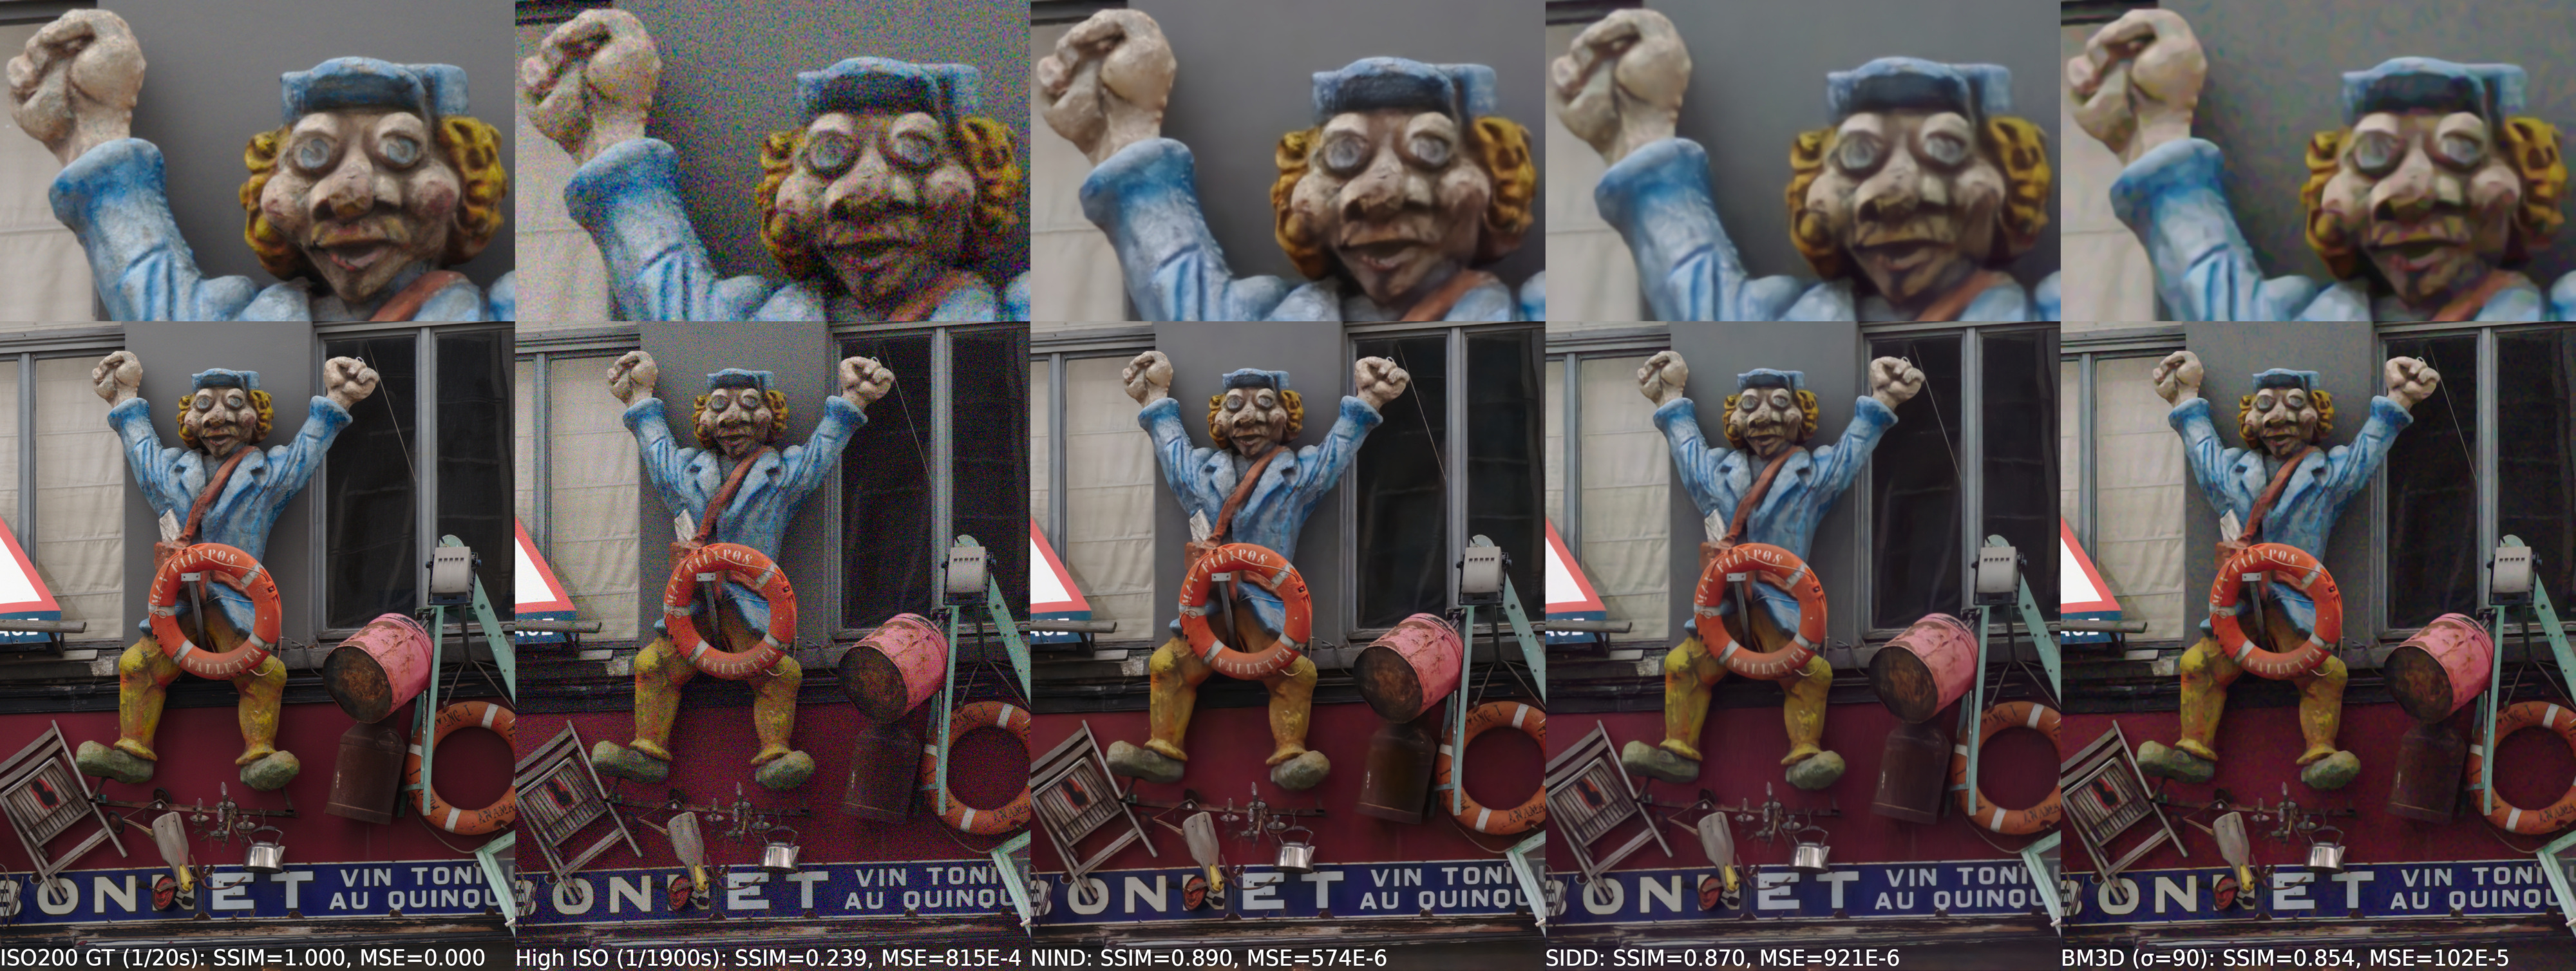
\includegraphics[width=1\linewidth]{gfx/comp/stefantiek.jpg}
\caption[Denoising stefantiek (visual comparison)]{Denoising stefantiek. 1: ISO200 ground-truth (1/20 s), 2: high ISO (1/1900 s), 3: 2 denoised using U-Net model trained with \ac{NIND}, 4: 2 denoised using U-Net model trained with \ac{SIDD} (320-sets), 5: 2 denoised using \ac{BM3D} ($\sigma=90$\footnoteref{sigmanote})}
\label{fig:stefantiek}
\end{figure*}

% \begin{figure}[!htbp]
% \centering
% 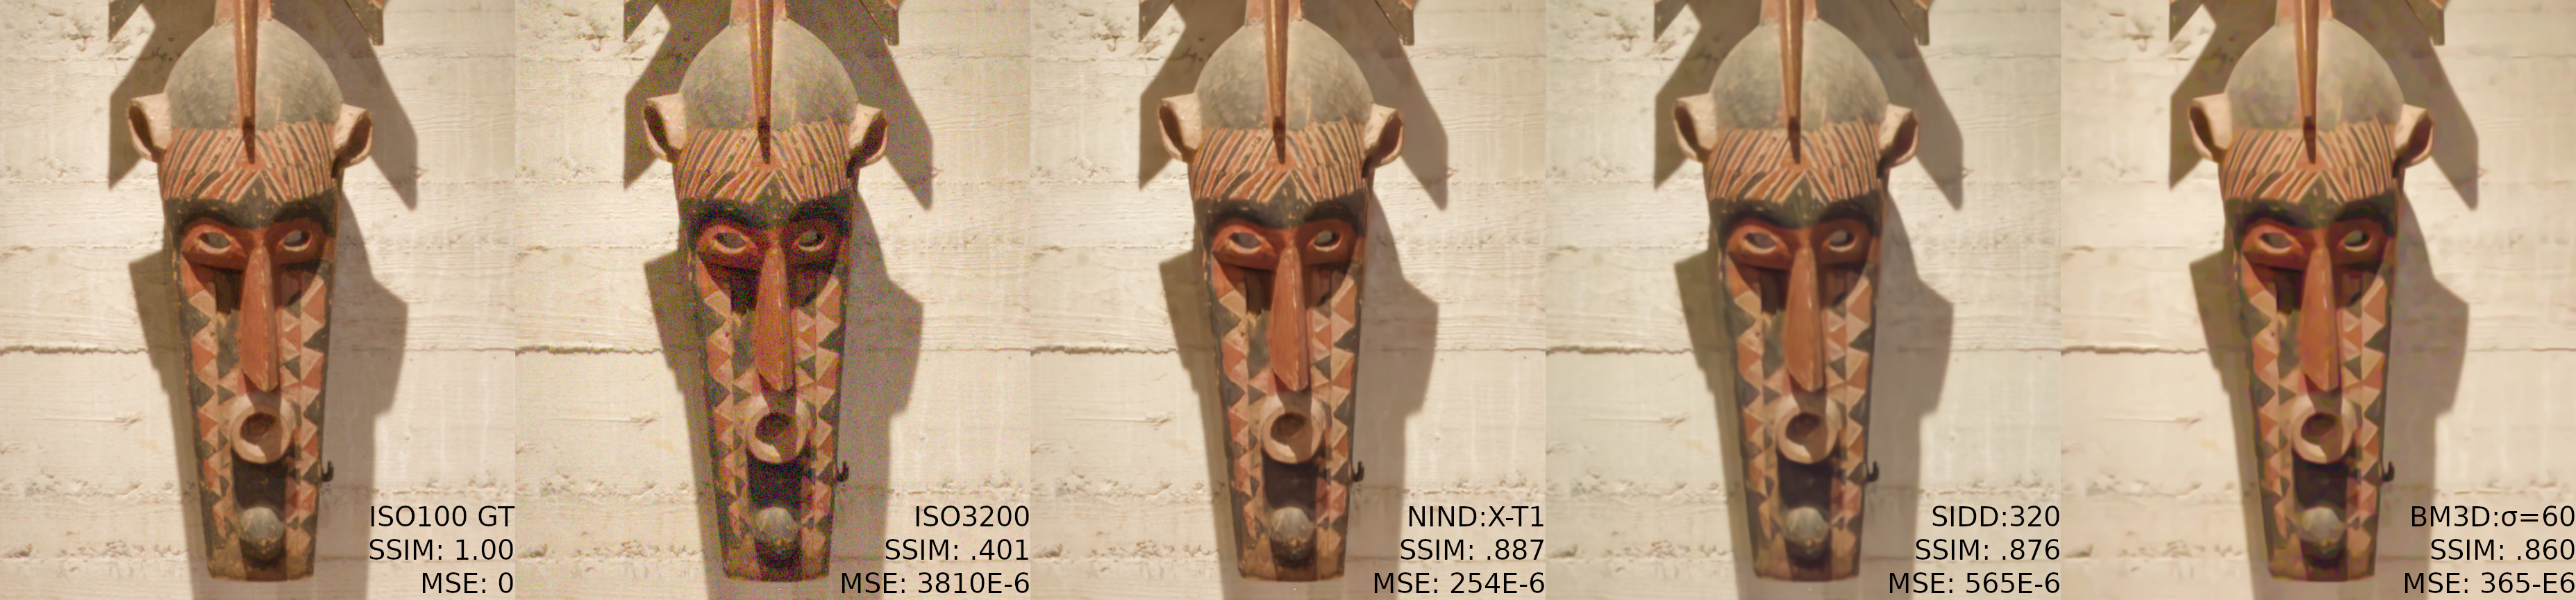
\includegraphics[width=1\linewidth]{../comp/NIND_MuseeL-Bobo-C500D.jpg}
% \caption{Denoising MuseeL-Bobo-C500D. 1: ISO100 ground-truth (4s), 2: ISO3200 (1/10s), 3: 2 denoised using U-Net model trained with \ac{NIND} (X-T1 subset), 4: 2 denoised using U-Net model trained with \ac{SIDD} (320-sets), 5: 2 denoised using BM3D ($\sigma=60$)}
% \label{fig:boboc500dvis}
% \end{figure}

\begin{figure*}[!htbp]
\centering
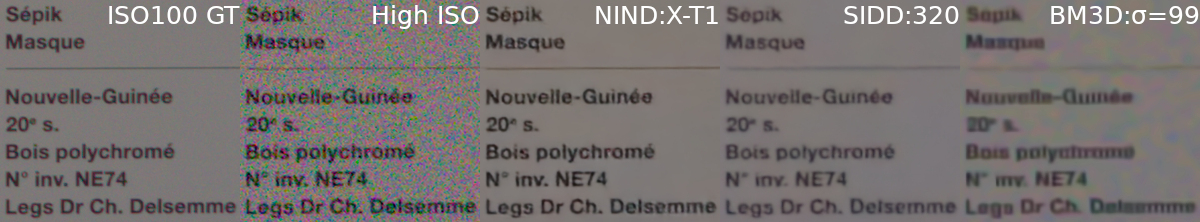
\includegraphics[width=1\linewidth]{gfx/comp/txt.jpg}
\caption[Denoising text present on MuseeL-Sepik-C500D (visual comparison)]{Denoising text present on MuseeL-Sepik-C500D. 1: ISO200 ground-truth (2 s), 2: high ISO (1/30 s), 3: 2 denoised using U-Net model trained with \acs{NIND}:\acs{X-T1}, 4: 2 denoised using U-Net model trained with \ac{SIDD} (320-sets), 5: 2 denoised using \acs{BM3D} ($\sigma=99$\footnoteref{sigmanote})}
\label{fig:text}
\end{figure*}

\begin{figure}[!htbp]
\centering
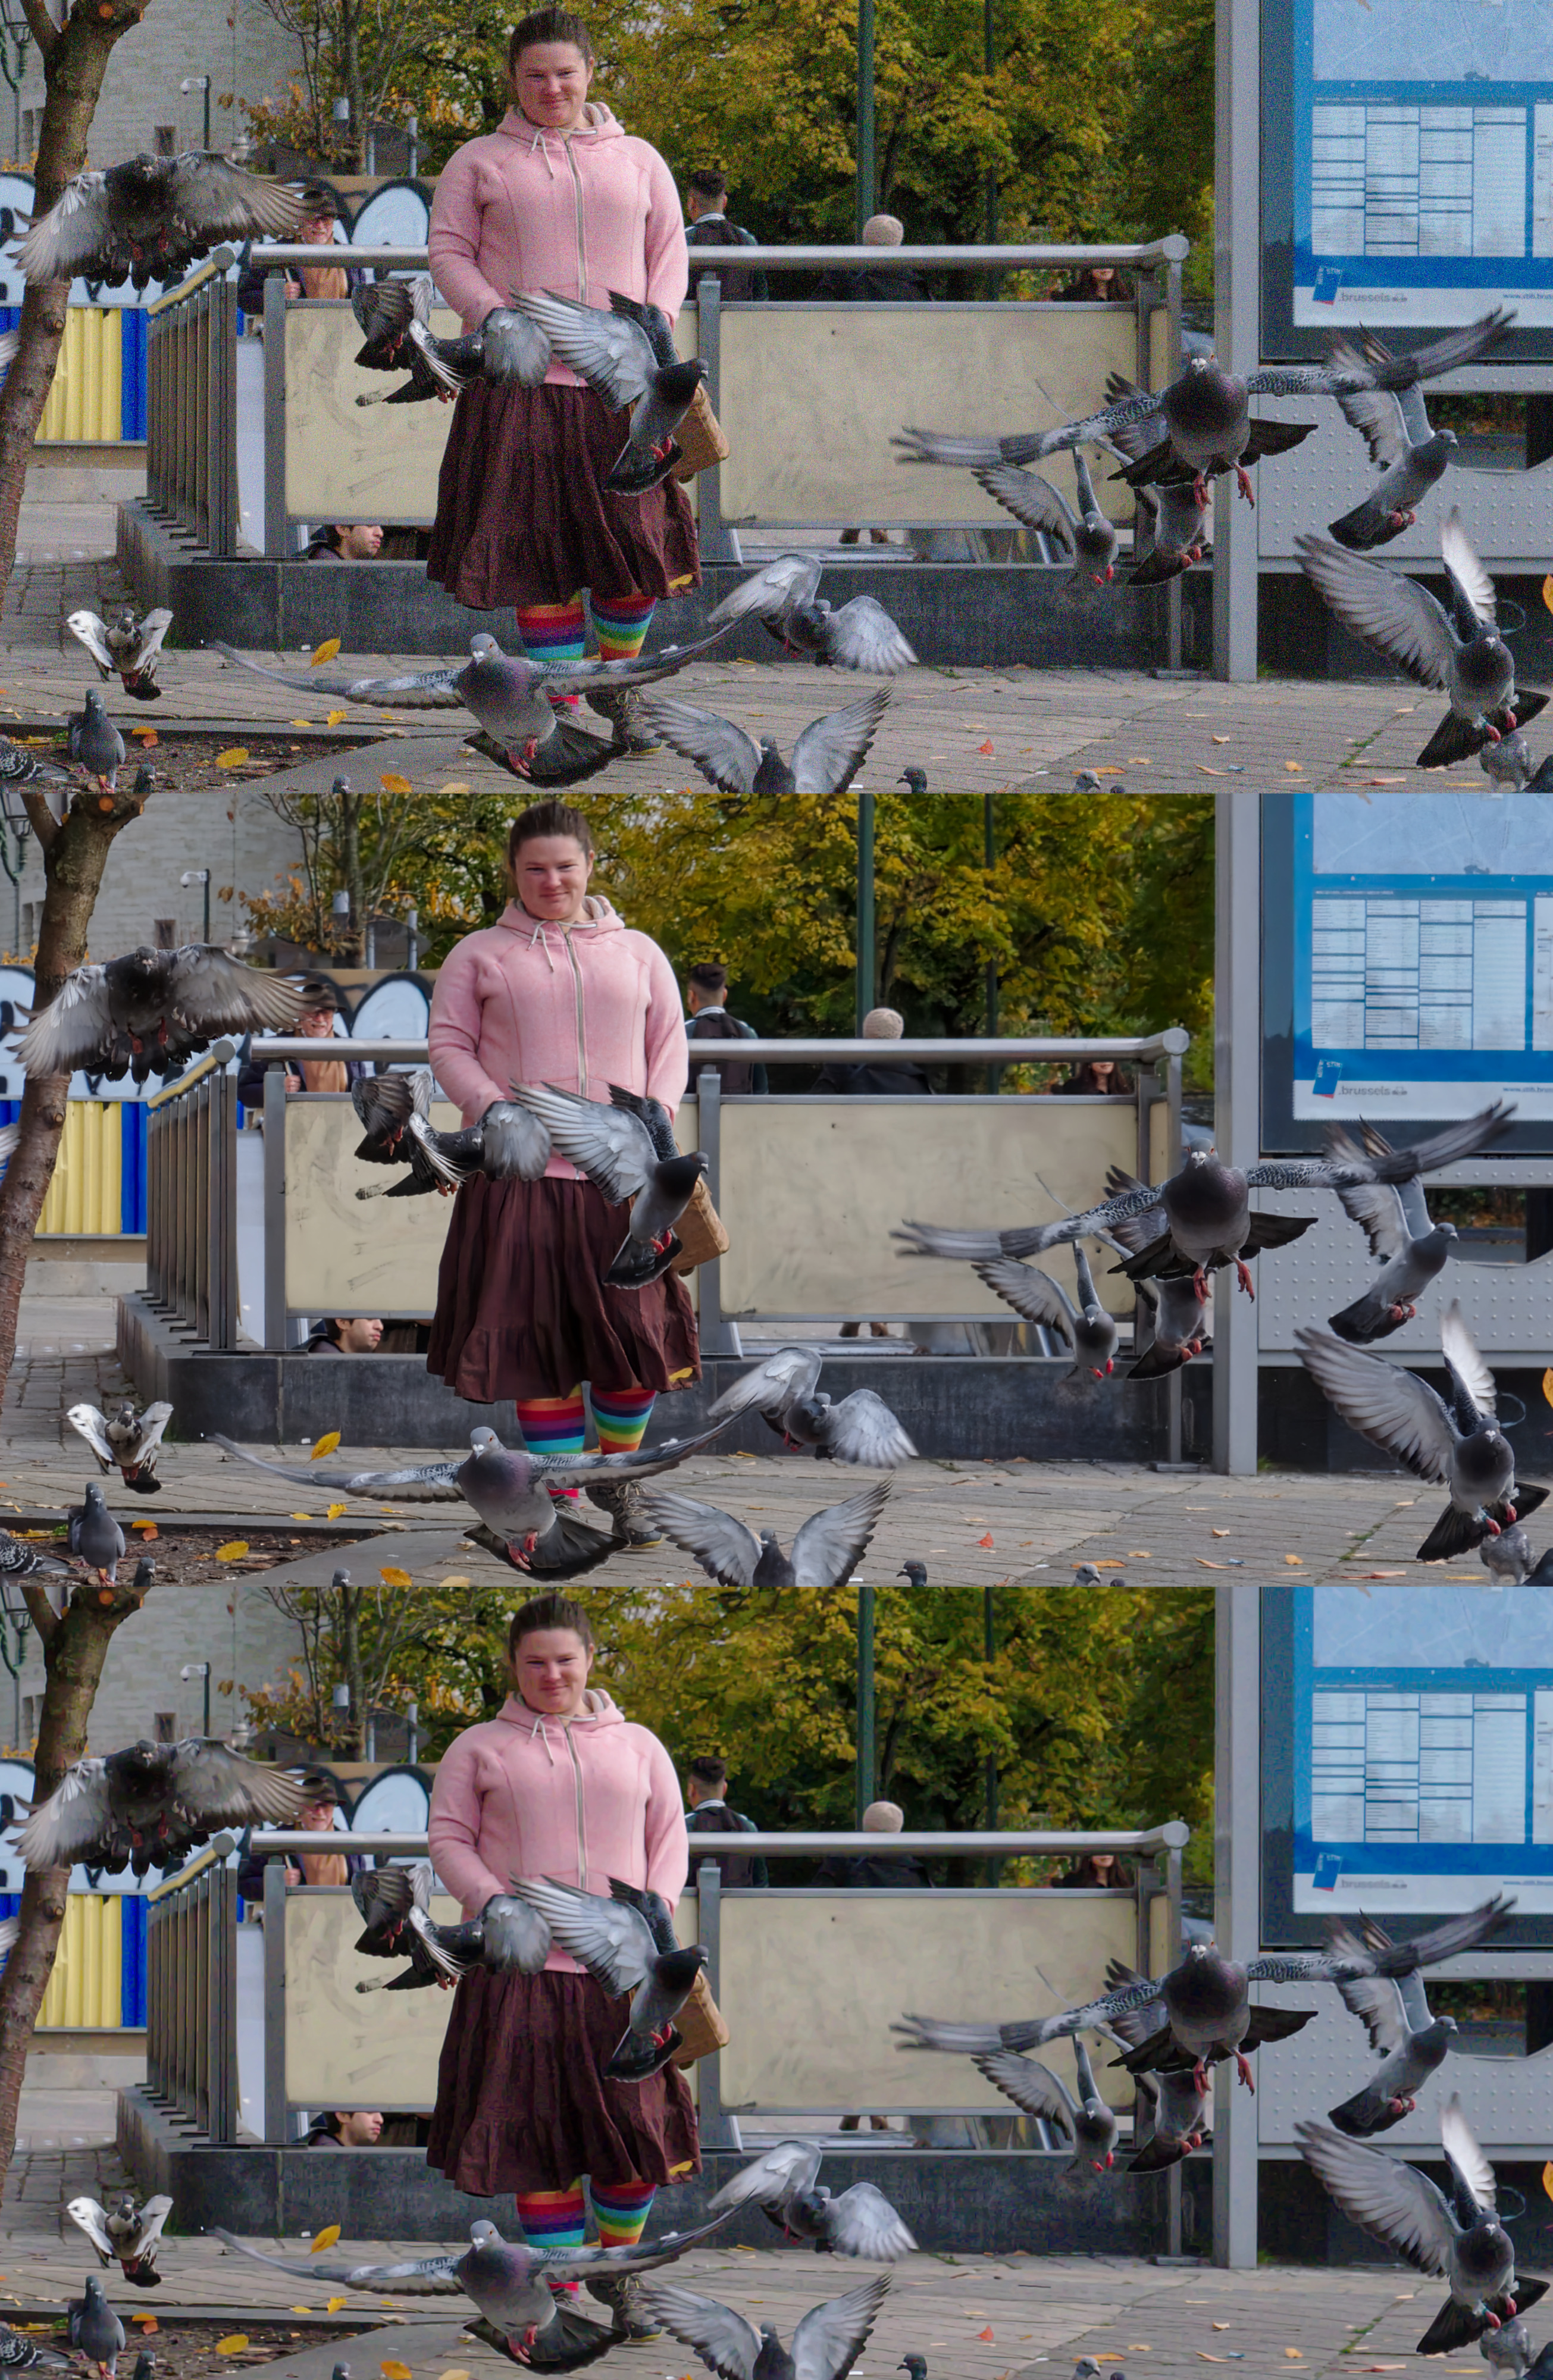
\includegraphics[width=1\linewidth]{gfx/comp/comp-noisy-nind-bm3d30.jpg}
\caption[Denoising of an unpaired "high-speed" image (visual comparison)]{Comparison between a noisy ISO6400 crop (top), one denoised with a model trained on \ac{NIND} (middle), and one on which \ac{BM3D} ($\sigma=30$) has been applied (bottom). Our model appears to perform well on dynamic scenes despite having been trained on static scenes.}
\label{fig:visualpigeons}
\end{figure}


Each network is trained for 48-hours on a GeForce GTX 1080 (11GB). % 77.1% of the time SIDD
Table \ref{tableNINDXT1} shows denoising performance on the Fujifilm X-T1 test pictures. We observe that the model trained on the \ac{NIND} significantly outperforms \ac{BM3D} and that adding training data from the Canon EOS 500D sensor, as well as part of the \ac{SIDD} dataset, does not appear to negatively impact performance. Table \ref{tableNINDXT1onBoboC500D} and Figure \ref{fig:boboc500d} show denoising performance on the scene ``MuseeL-Bobo-C500D", where a model trained only with \ac{NIND}:\ac{X-T1} data performs nearly as well as a model that was also trained with \ac{NIND}:\ac{C500D} data (and so does a model trained with both \ac{NIND} and \ac{SIDD}). Table \ref{tableXT1onC500D} summarizes the average performance of \ac{X-T1}-trained models on ten \ac{C500D} scenes and shows performance which considerably exceeds that of \ac{BM3D} even though the model was generalizing for a different sensor type.

A model trained with only \ac{NIND}:\ac{X-T1} ISO6400 noisy images yields slightly better performance at and around ISO6400, but this comes with a considerable loss of detail at low ISO and the denoising performance becomes poor as the noise level increases. Moreover the model trained on Fujifilm X-T1 ISO6400 images appears not to generalize as well to different sensors as we found it consistently performs worse on the Canon 500D images. These findings suggest that the cost of generalization is acceptably low and therefore a model mostly benefits from learning with different noise levels and sensors.

Reconstructing the noise (Method \ref{exp:nindmakenoise}) as was suggested in \cite{dncnn} typically yields performance below that of BM3D when applied to ISO noise. The difficulty in reconstructing ISO noise was further noticed in an experiment where we mistakenly fed our learning model noisy images as ground-truth 31\% of the time and it still exceeded BM3D performance. This went as far as inverting the clean and noisy crops and still learning an appreciable level of denoising. These findings suggest that a model can easily tolerate some noise in the ground-truth data. Research into this topic \cite{noise2noise}  has been performed to explicitly train models on noisy data and rely on the zero-mean nature of the noise to effectively remove various artificial noise distributions.

Training a model using artificial noise added to ground-truth images (Method \ref{exp:nindart}), as is commonplace in the literature \cite{rednet}\cite{dncnn}, yields the worst performance in our tests.

Figure \ref{fig:text} shows satisfying denoising performance of a model trained on \ac{X-T1} images with text recovered from a \ac{C500D} image. In addition to the aforementioned results based on \ac{SSIM}, we have subjectively tested our \ac{NIND}-trained model on single images which are not part of the dataset. The first such image is that of a dynamic outdoor scene in which a human walks towards a group of pigeons, causing them to disperse in multiple directions. This type of fast, moving scene cannot be included in the dataset due to its dynamic nature and it must be captured with settings that result in a poor quality image; a small aperture (f/11) to focus everywhere, a fast shutter speed (1/1500 s) to capture the flying birds, and a maximum sensor sensitivity (ISO6400) to match the aforementioned settings. Nonetheless, we found the denoised image to be of high quality; we submitted it to the Wikimedia Commons ``Quality Images Candidates" page \cite{qic} and it was subsequently promoted to a ``Quality Image" by Wikimedia Commons reviewers. A crop of the image is provided on Figure \ref{fig:visualpigeons} with a comparison between the noisy version, one denoised with a U-Net model trained on \ac{NIND}, and a version that has been denoised using \ac{BM3D} (with $\sigma=30$ which, on average, yields the highest \ac{SSIM} in our ISO6400 test images). The BM3D version shows significant displeasing artifacts, for example on the skirt and the blue uniform panel on the right, while the model trained on \ac{NIND} smoothed these regions appropriately while retaining a greater level of useful details such as those present on the pigeons' wings.

%%%%%%%%%%%%%%%%%%%%%%%%%%%%%%%%%%%%%%%%%%%%%%%%%%%%%%%%%%%%%%%%%%%%%%%%%%%%%%%%%%%%%%%%%%%%%%%
%%%%%%%%%%%%%%%%%%%%%%%%%%%%%%%%%%%%%%%%%%%%%%%%%%%%%%%%%%%%%%%%%%%%%%%%%%%%%%%%%%%%%%%%%%%%%%%
%%%%%%%%%%%%%%%%%%%%%%%%%%%%%%%%%%%%%%%%%%%%%%%%%%%%%%%%%%%%%%%%%%%%%%%%%%%%%%%%%%%%%%%%%%%%%%%

\section{GAN Denoising}\label{sec:GAN Denoising}

We initially trained denoising networks using the pix2pix approach (the typical use-case is generating photorealistic images from rough sketches) of performing image to image translation using a PatchGAN discriminator and a U-Net generator \cite{pix2pix}. The results were not satisfying even after applying the adjustments mentioned in section \ref{sec:Initial training method}; the PatchGAN would consistently prefer high frequencies and the denoising performance suffered. We thus designed our own HulDisc discriminator and a similar HulbNet generator and tested their individual building blocks in section \ref{sec:Components} before assessing the system as a whole and comparing it to previous approaches in section \ref{sec:System as a whole}.

\subsection{PatchGAN}

We first tried following the pix2pix approach using a PatchGAN discriminator and a U-Net generator \cite{pix2pix} with 1:3 training ratio. The discriminator handles high-frequency details and low-frequencies are handled by the $\ell 1$ loss. We were unable to obtain satisfying performance after experimenting with different loss balances, we found that the denoising performance was subpar to that of \ac{BM3D} and of our previous U-Net network; high-frequencies tend to be exaggerated in low-frequency areas and high frequency details are not properly recovered, often resulting in an overall poor \ac{SSIM} index. Figure \ref{fig:p2p-def} illustrates the denoising performance obtained using a 0.25 $\ell 1$ multiplier.

\begin{figure}[!htbp]
  \begin{center}
    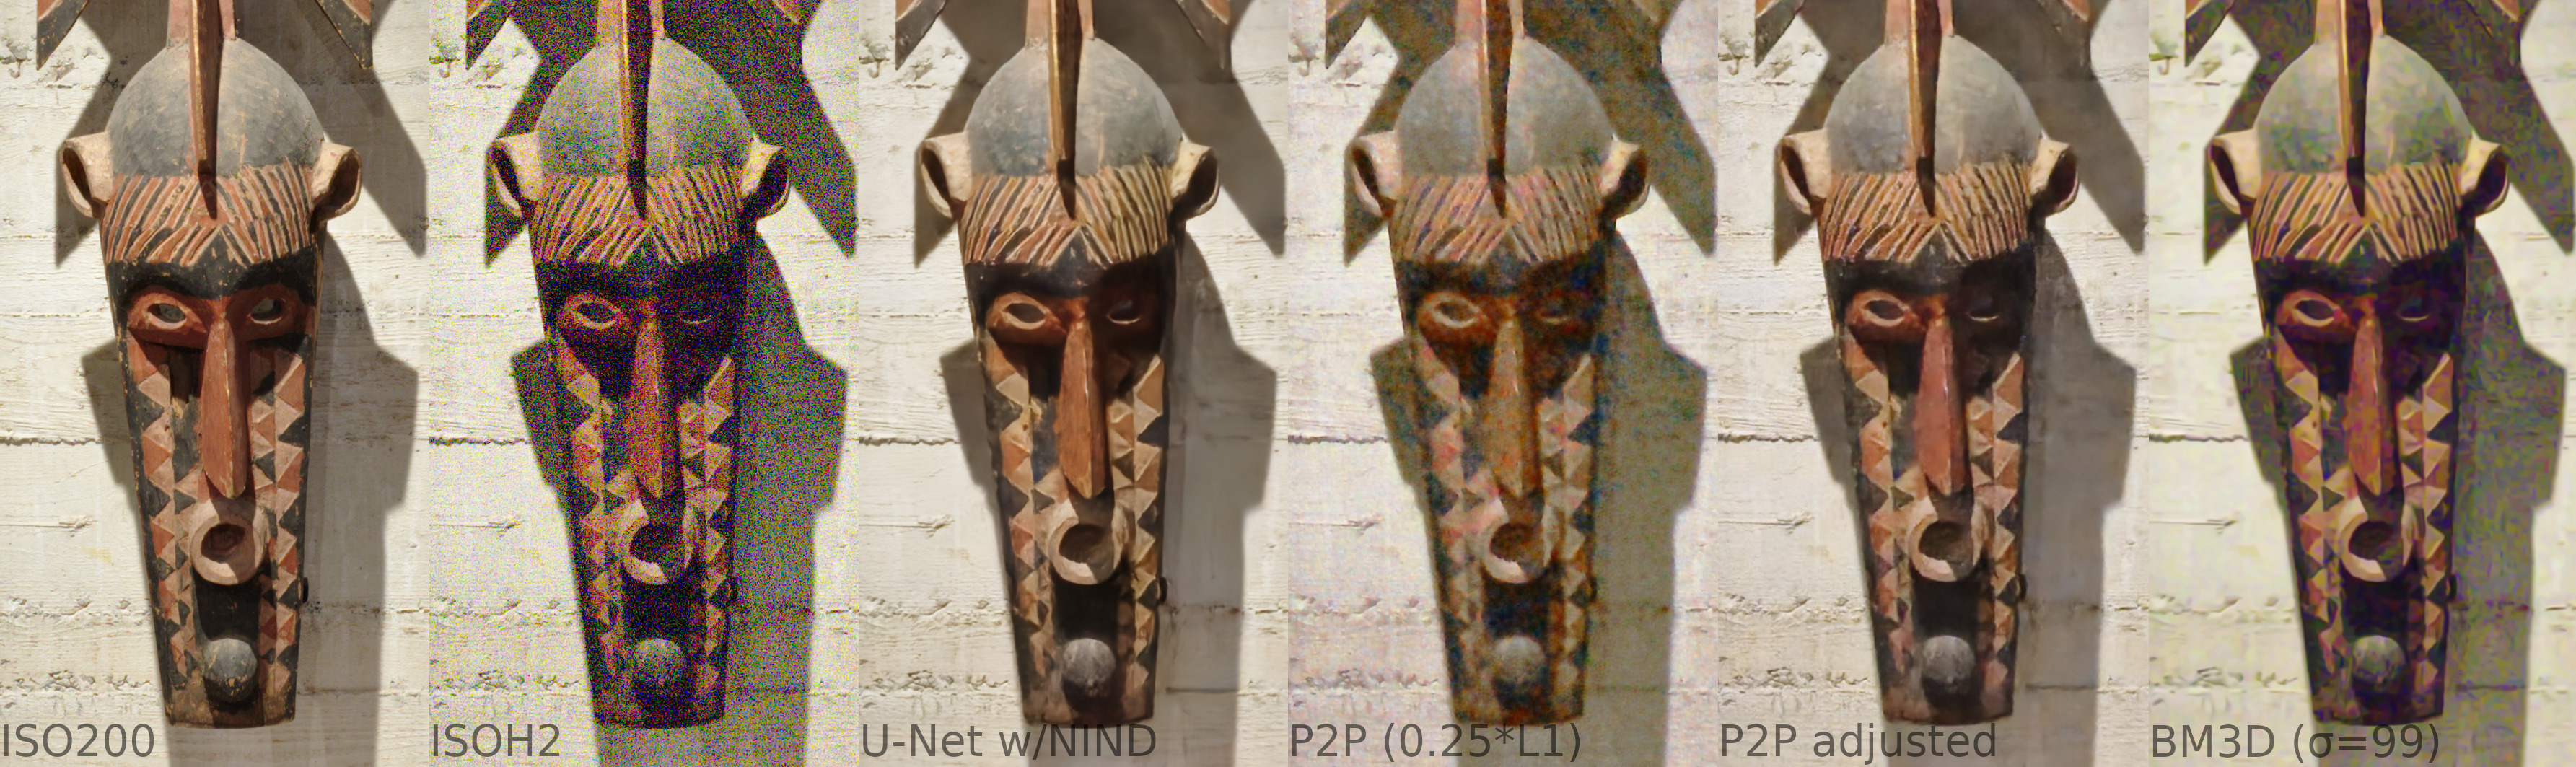
\includegraphics[width=1\linewidth]{gfx/comp/p2p_def.jpg}
    \caption[Initial (c)GAN denoising (visual comparison)]{Comparison of standard pix2pix \cite{pix2pix} applied to image denoising with other methods on a crop from image NIND\_MuseeL-Bobo\_ISOH2. 1: ISO200 ground-truth crop (SSIM: 1.00), 2: ISOH2 noisy crop (SSIM: 0.151), 3: Denoised image with a single U-Net network trained on the \ac{NIND} (SSIM: 0.810), 4: Denoised image with a standard pix2pix network trained on the \ac{NIND} with $0.25\times\ell 1$ (SSIM: 0.672), 5: Denoised image with a pix2pix network trained on the \ac{NIND} with the following adjustments: minimum of 35 iterations with $\text{loss}_\text{SSIM} < 0.125$ before using the discriminator with $\text{loss}_G=0.5 \text{loss}_D + 0.4 \text{loss}_\text{SSIM} + 0.1 \text{loss}_{\ell 1}$ (SSIM: 0.794),6: Denoised with \ac{BM3D} using $\sigma=99$ (SSIM: 0.694)}
    \label{fig:p2p-def}
  \end{center}
\end{figure}

Some improvement were made with careful fine-tuning of the learning environment. We added the \ac{SSIM} loss used in single-network training and tested different balances between the $\ell 1$, \ac{SSIM}, and discriminative losses. We tried training the generator without applying a discriminative loss until a SSIM threshold is met for a given number of consecutive iterations, and we tried training a non conditional network. Figure \ref{fig:p2p-comp-1} shows performance on the "stefantiek" set using different settings on a non conditional network (as well as the baseline network performance without these adjustments). We observe particularly poor performance when the discriminative loss has a high weight (weight\_D = 0.9), as well as when we start using the discriminative loss early on before the generator has learned to properly denoise with the conventional loss functions (min\_SSIM=0.3). The GAN network obtains reasonable performance when the generator is pretrained to achieve a \ac{SSIM} loss of 0.125 to 0.15. The greatest performance shown occurs when the generator has to obtain $\text{loss}_\text{SSIM} < 0.125$ for 35 consecutive iterations before using the discriminator as half of the overall loss. A crop denoised with this model (5) is shown beside one trained with standard pix2pix \ac{cGAN} (4) on Figure \ref{fig:p2p-def}.

\begin{figure}[!htbp]
\centering
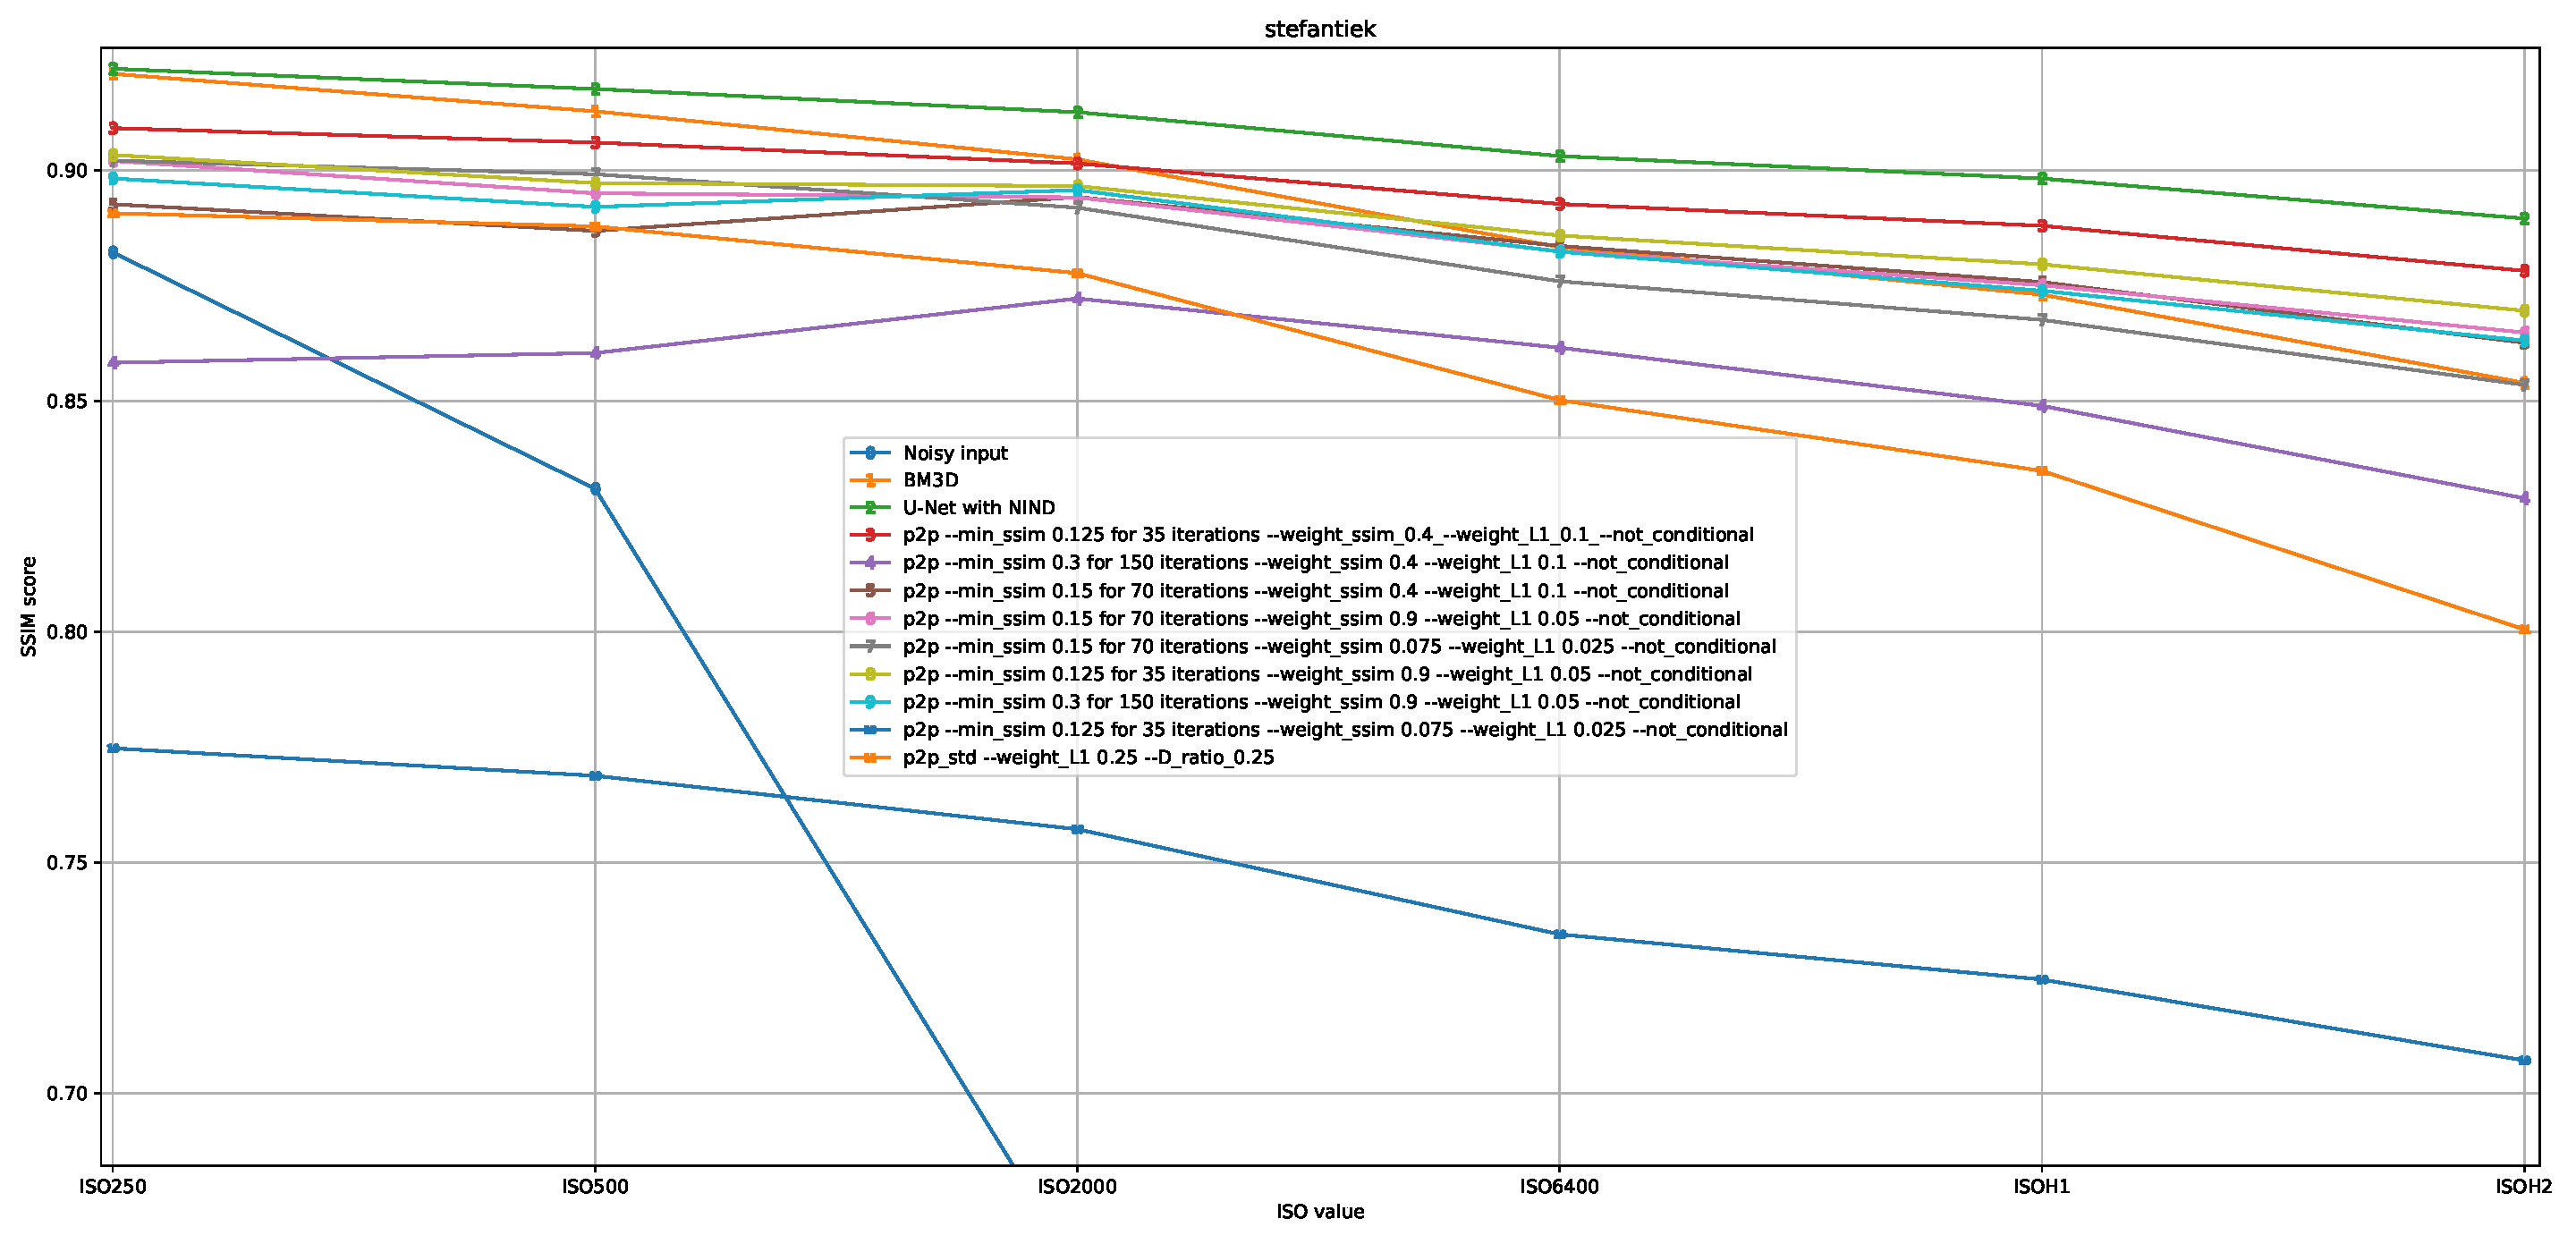
\includegraphics[width=1\linewidth]{gfx/graphs/p2p-comp-1.pdf}
\caption[Denoising performance of \acsp{GAN} on the "stefantiek" set]{Denoising performance of the non conditional GAN with varying weights and schedules on the "stefantiek" set over increased ISO values. The models appear to perform better when they are pre-trained to achieve good performance with the \acs{SSIM} loss before taking the discriminator's feedback into account, and when the discriminator's weight (1 - other weights) does not account for the bulk of the loss function.}
\label{fig:p2p-comp-1}
\end{figure}

\subsection{Our proposed architecture}
\subsubsection{Components}\label{sec:Components}
Our main motivation for designing the "Hul" architectures described in sections \ref{HulbNet} and \ref{HulDisc} is the poor performance obtained with a PatchGAN discriminator; the discriminative network should not focus only on high-frequencies or its feedback becomes corruptive. We also wanted to replace the U-Net generative network which loses too much border that is either easily discriminated against or that does not leave a large enough crop for the discriminator to make up meaningful results. We thus designed both a generator and a discriminator which follow the same design ideas (alas the discriminator is cut in half and thus loses many of the dense connections), and tested specific components for their respective use-cases.
%Network like \cite{pix2pixhd} which processes multiple scales to capture high-frequencies and smooth textures. Instead of dividing up the images into different resolutions or using multiple networks, we followed an approach similar to that of DenseNet \cite{densenet} which concatenates multiple channels together from different layers (as opposed to summing the features \cite{resnet}), allowing layers to contain different types of features captured with different convolutions. Some of the convolutions thus capture a wider receptive field using dilation which has been shown to perform well in image segmentation tasks \cite{multi-scale-dilation}, while other channels focus on local details with standard convolutions.

%At the same time we wanted to replace the U-Net network which loses too much border that is either easily discriminated against or does not leave a large enough crop for the discriminator to make up meaningful results. We thus designed both a generator and a discriminator which follow the same design ideas (alas the discriminator is cut in half and loses many of the dense connections), and tested specific components for their respective use-cases.

The two architectures were trained separately to assess and optimize their individual performance before working together. The generator is typically trained using the same framework as that of section \ref{sec:CNN Denoising}, while the discriminator main tests involve discriminating between clean and noisy crops from the dataset without receiving the conditional input. This test is not as robust as training with the result of a static generator but it allows us to quickly get a preview of the discriminator's performance whereas it would not always be able to learn from scratch given a well trained generator.

\begin{figure}[!htbp]
\centering
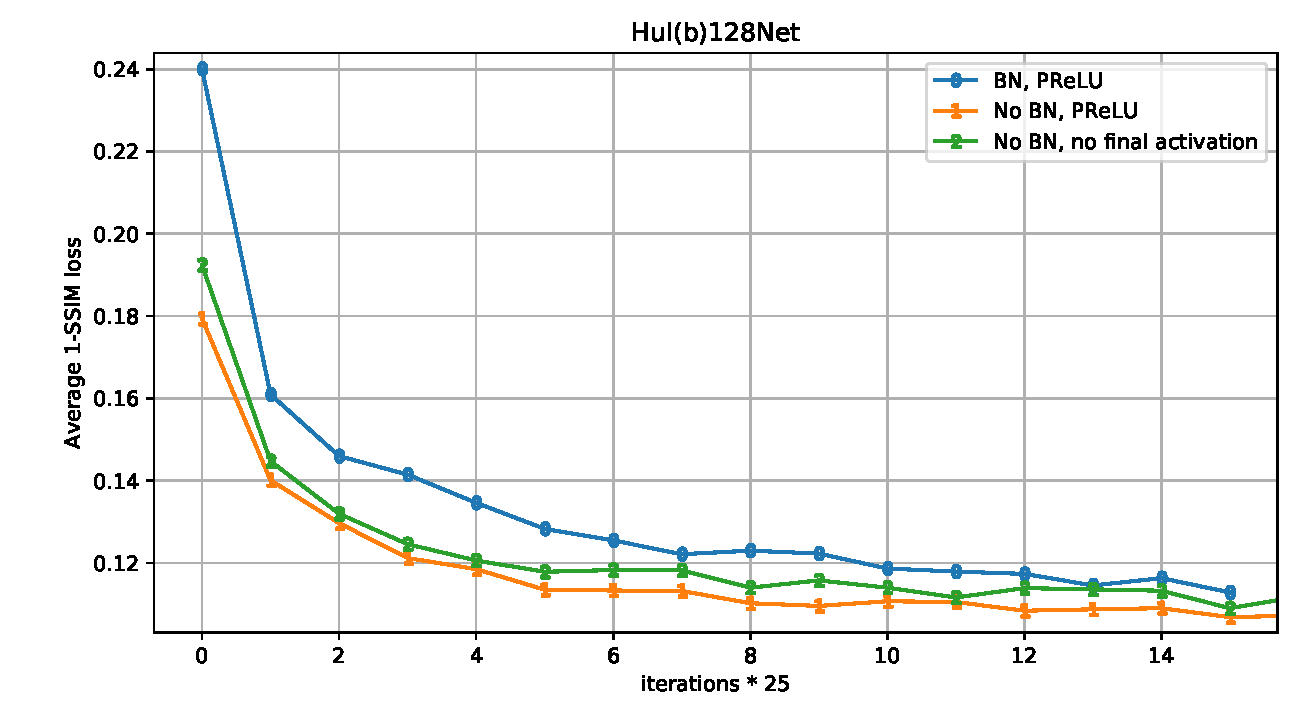
\includegraphics[width=1\linewidth]{gfx/graphs/gen-BN.pdf}
\caption[Generative network learning curve with and without batch normalization]{Generative network learning curve with and without \acl{BN} ("HulbNet"), as well as with neither \ac{BN} nor an activation function. We observe better performance when \acl{BN} is not applied and with the use of a non-linear final activation function.}
\label{fig:gen-BN}
\end{figure}

\acl{BN} appeared to hamper learning on the generative networks, often yielding worse color rendition and lowering the \ac{SSIM} index (which does not appear to be very sensible to color accuracy). We trained a generative network for an epoch with and without batch normalization to finally determine whether \ac{BN} should be removed from the generative network. Figure \ref{fig:gen-BN} shows the resulting learning curve, which allows us to confidently remove \ac{BN} from the generative architecture (we add the letter b such that "HulbNet" denotes a network without \ac{BN}). We also trained a network for an epoch to determine whether not using a final loss function as is sometimes done \cite{dncnn} would yield better performance than \ac{PReLU}, but we found the network performs better with a non-linear activation function.

% TODO fix imbalance
% TODO explicitly mention loss
\begin{figure}[!htbp]
\centering
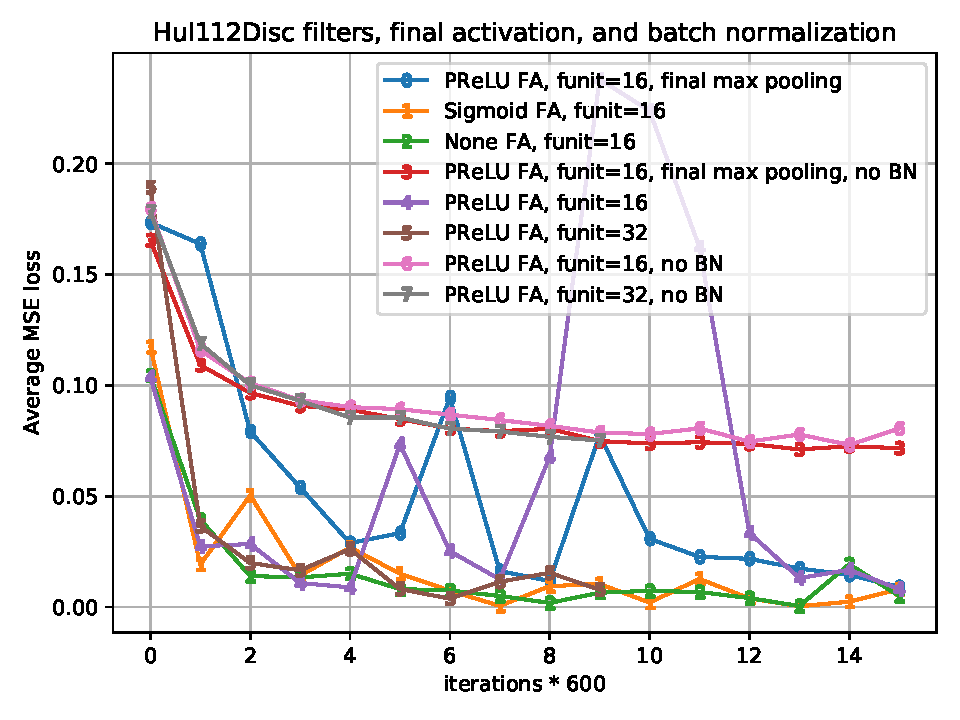
\includegraphics[width=1\linewidth]{gfx/graphs/hul112disc-activ.pdf}
\caption[Discriminative network learning curve with different final activation functions and number of filters]{Discriminative network learning curve with varying final activation functions (FA) and number of filters. We observe that the discriminative network benefits greatly from \ac{BN} and that training stability and performance suffer from not having a sufficient number of filters. One funit denotes the number of filters multiplier (with the first layer outputting two funits). The network is not conditioned and its task is to discriminate whether an image is clean or noisy. The loss is squared therefore a \ac{MSE} of 0.25 is equivalent to guessing 0.5.}
\label{fig:hul112disc-activ}
\end{figure}

% TODO add hulfdisc
Figure \ref{fig:hul112disc-activ} shows the discriminator's learning curve classifying images as either clean or noisy. We observe that \acl{BN} is useful in the case of the discriminator, likely because its job does not entail recreating image fidelity from the input but output a single probability, and \acl{BN} can help when given mini-batches of a single target value (line 3, 6, 7). We observe that the \ac{PReLU} activation function yields sporadically very poor performance on line 0 and 4, but performance is restored with a greater number of filters. Ending the discriminative network with a final max-pooling appears worse than a learned convolution. The different activation functions seem roughly equivalent as they overtake one other over time. Although we observe the importance of using a sufficient number of filters, we cannot conclude an actual number of needed filters from this experiment because the task is simpler than discriminating between real (baseline) and fake (denoised) images, but the real task at hand cannot be accomplished because the discriminator never catches up if there is a large discrepancy between an untrained discriminator and a pre-trained generator.

\begin{figure}[!htbp]
\centering
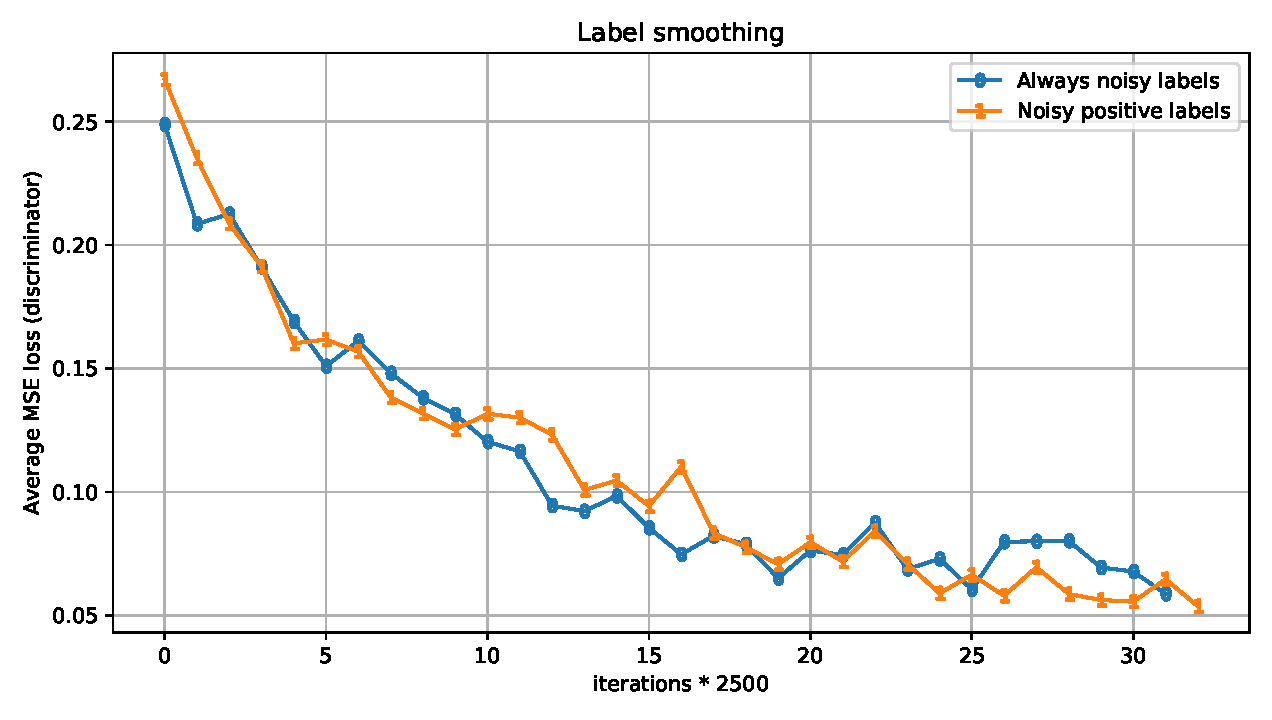
\includegraphics[width=1\linewidth]{gfx/graphs/label-smoothing.pdf}
\caption[Discriminative network performance with noisy labels (always noisy or noisy for positive labels only)]{Discriminative network performance (\ac{MSE} loss) with noisy labels (either always noisy or noisy for positive labels only). The network attempts to discriminate images denoised by a generator which has been trained for three epochs and is continuously being updated (alas without any input from the discriminator). We did not observe a notable difference in performance between the two label smoothing methods.}
\label{fig:label-smoothing}
\end{figure}

Following some incertitude on whether label smoothing should only be applied on positive labels as per \cite{gantechniques} or on all batches used to train the discriminator, we compared the two approaches and show the results on figure \ref{fig:label-smoothing}. The test protocol is different from the previous one in that the discriminator attempts to discriminate against images denoised by a generator which has been pre-trained for three epochs (and is continuously being updated, although it receives no feedback from the discriminator). The results we observed did not seem to differ significantly as the two discriminators would continuously overtake one other.

% switching losses is bad
\subsubsection{System as a whole}\label{sec:System as a whole}

In this section we test different configurations of our "Hul" \ac{cGAN} networks as a whole system trained according to our trained method described in section \ref{sec:Adopted training method}. The performance is compared to the previously used configurations as well (U-Net alone and the PatchGAN), and we assess the visual quality of denoised images where it was previously lacking (i.e. noisy face images).

The different types of network present in this experiment are as follow:
\begin{itemize}
  \item Hul is the base name of the network we use
  \item b: no batch normalization
  \item f: more channels as the other dimensions decrease
  \item A number representing the minimum valid input size
  \item Disc for discriminators or Net for generators
\end{itemize}

\begin{figure}[!htbp]
\centering
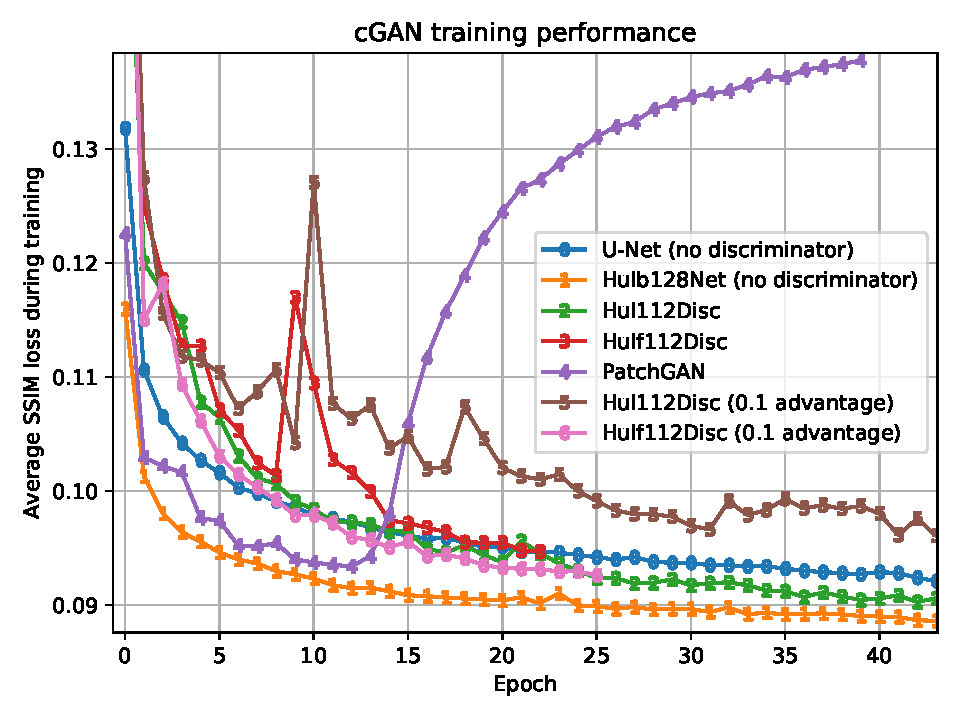
\includegraphics[width=1\linewidth]{gfx/graphs/cgan-comp.pdf}
\caption[cGAN learning curve]{
cGAN training performance comparison. 0: The U-Net model from experiment \ref{sec:CNN Denoiser}:\ref{exp:nindxt1}, 1: Hulb128Net (without a discriminator). The following networks all use the Hulb128Net generator and a specified discriminator. 2: Hul112Disc, 3: Hulf112Disc (more filters as the network shrinks), 4: PatchGAN \cite{pix2pix}, 5: Hul112Disc which learns 10 \% more often than the generator, 6: Hulf112Disc which learns 10 \% more often than the generator.
Our HulbNet generator appears to outperform U-Net both as a single network and in a \acs{GAN}. Although the \acs{cGAN} system appears to perform better, that is expected because the main loss is no longer based on a correlation with the ground-truth image, and visual analysis of the results later confirm that the \acs{cGAN} system offers more visually pleasing denoising. Adding more filters to the discriminator appears to only work if the discriminator has a higher training ratio to optimize them. Likewise, a discriminator that is trained more often does not appear to offer a better feedback if its capacity is not high enough.}
\label{fig:cgan-comp}
\end{figure}

% generate faces, graph on an image

The networks' training performance is shown on figure \ref{fig:cgan-comp}. The baseline is a single generative U-Net network, and we also trained a single Hulb128Net network. The single Hulb128Net network appears to perform better than the U-Net of our previous experiments. We observe that the increased number of filters (Hulf112Disc) destabilizes the discriminator, but performance is restored when the discriminator has more time to learn. On the other hand, giving more time to a discriminator (0.1 advantage) that does not have as much capacity provides worse feedback and the result of the generator suffers. The PatchGAN's performance seems to degenerate quickly, and the Hulb128Net alone offers greater performance than that of a \acs{cGAN} pair but further analysis shows that the \acs{cGAN} denoised images are visually superior. The networks that were trained for longer benefit greatly from the additional time and exceed the performance of a single U-Net generator which maxes out at \acs{SSIM} index = 0.902. The \acs{SSIM} training loss is shown. Although \acs{SSIM} is not a meaningful enough factor on its own because the network could recreate a structurally different yet visually pleasing image, it provides an approximate indicator of performance and learning.

All \ac{cGAN} networks use a $\text{loss}_{\ell 1}$ weight of 0.05 and a $\text{loss}_\text{SSIM}$ weight of 0.2. While it may be worth trying different ratios, we found that the networks quickly became unstable as the weight of the discriminative loss increased; a $\text{loss}_\text{discriminative}$ weight of 0.95 would typically not complete the first epoch.


\begin{figure}[!htbp]
\centering
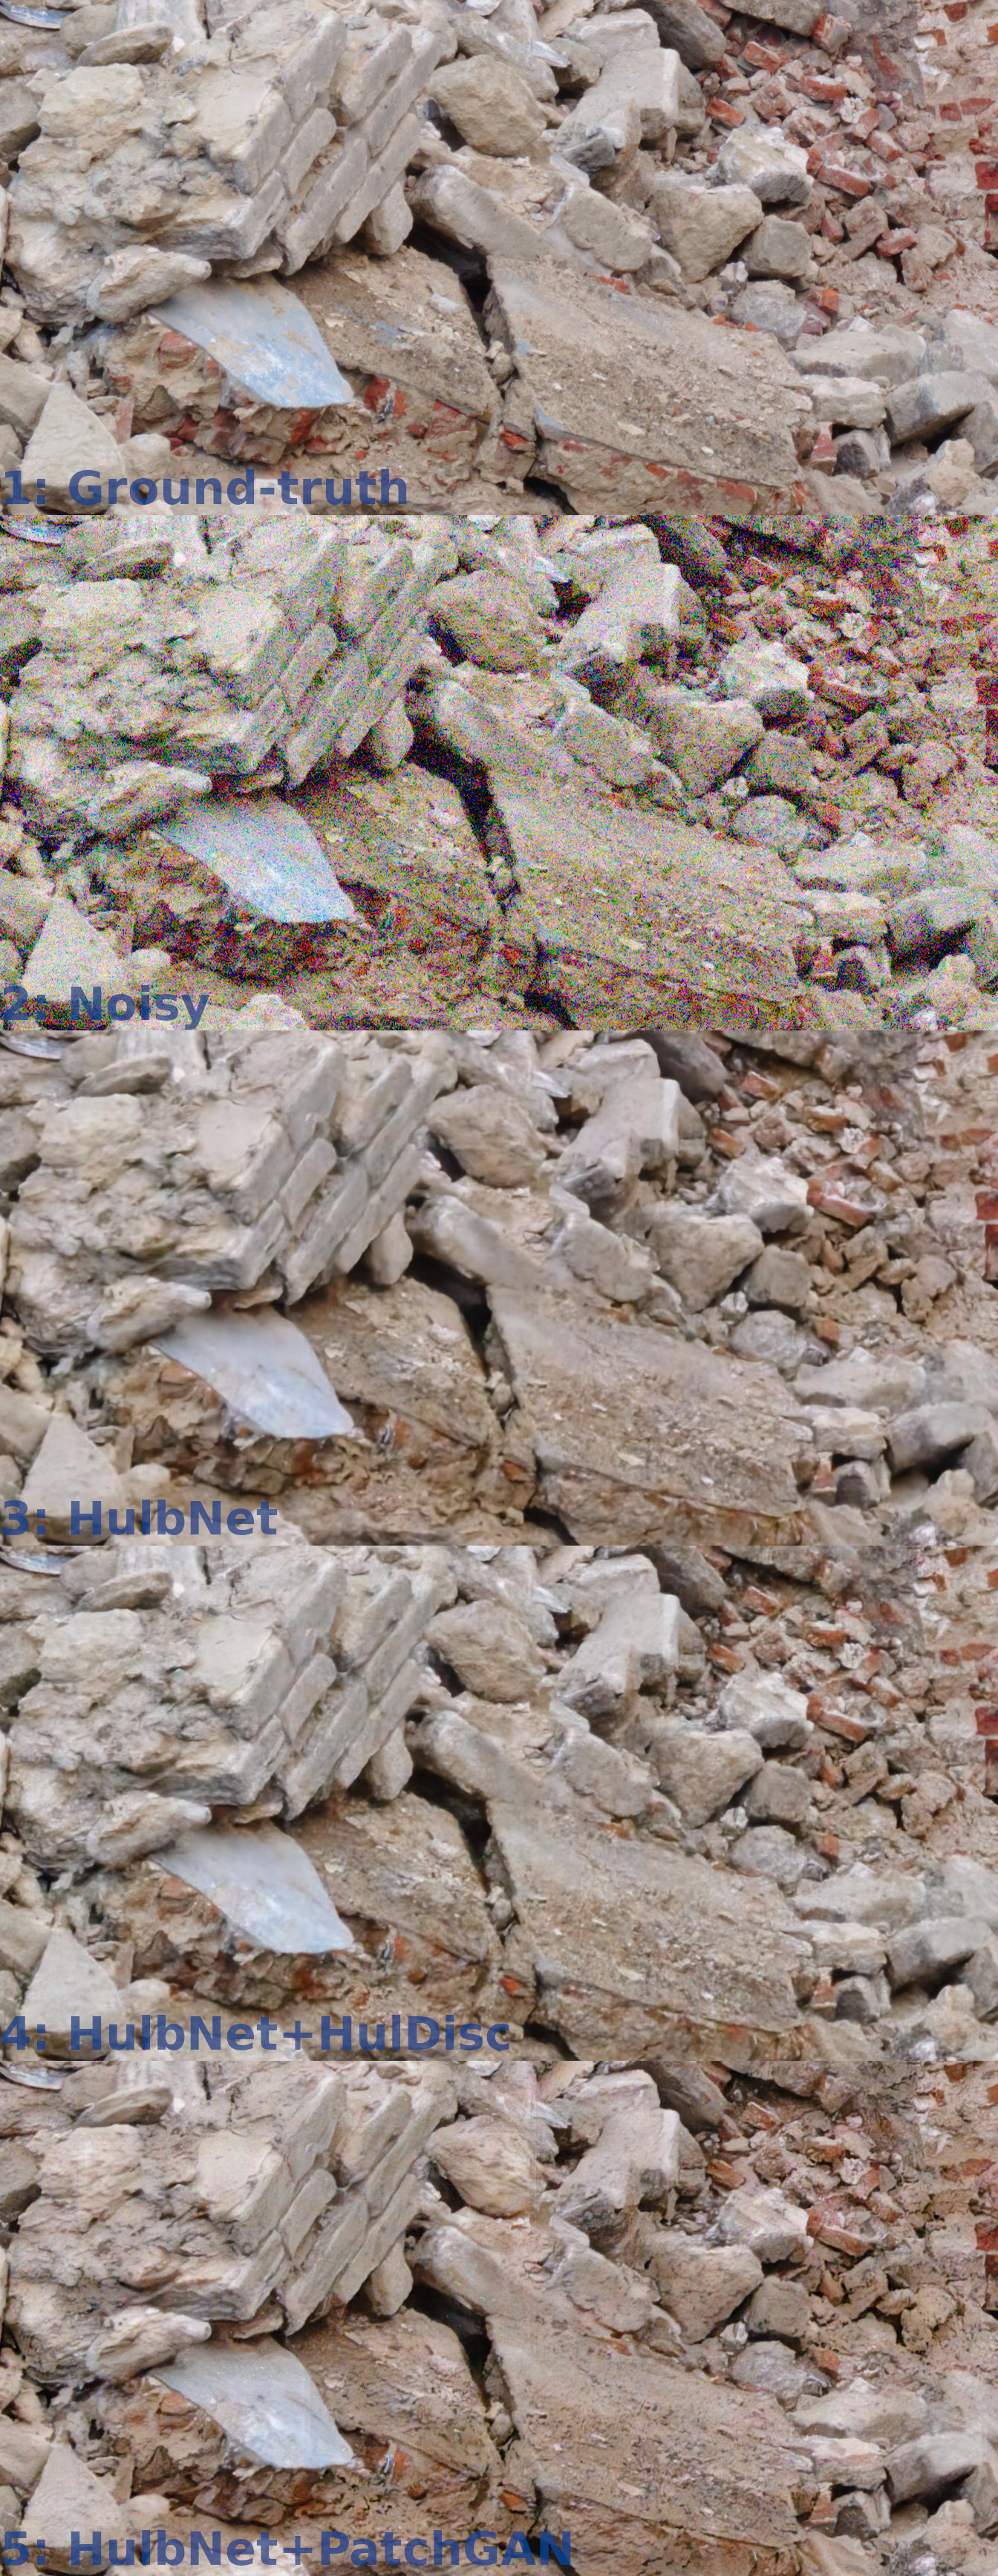
\includegraphics[width=1\linewidth,height=0.9\textheight,keepaspectratio]{gfx/comp/NIND_CourtineDeVillersDebris_ISOH2-cgan.jpg}
\caption[Denoising CourtineDeVillersDebris with cGANs (visual comparison)]{Visual comparison of different networks' denoising performance on NIND\_CourtineDeVillersDebris\_ISOH2. 1: Ground-truth (ISO200 1/4 s, SSIM: 1.000), 2: Noisy (High ISO 1/1100 s, SSIM: 0.232), 3: HulbNet generator with no discriminator (SSIM: 0.784), 4: HulbNet generator and HulDisc discriminator (SSIM: 0.780), 5: HulbNet generator and PatchGAN discriminator (SSIM: 0.687).}
\label{fig:cgan-wall}
\end{figure}

Figure \ref{fig:cgan-wall} visually shows the denoising performance of various \ac{cGAN} and conventional networks. We only displayed one combination of "Hul" generator-discriminator pair because we could not discern an appreciable difference between any of our trained \ac{cGAN} models. We observe restored high frequencies in the \ac{cGAN} network, whereas the single generator does not provide as much detail. The PatchGAN offers a very sharp image but much of the generated image looks unnatural (and the bricks in less chaotic parts of the image have an asymmetrical structure). The SSIM index does not correlate with a visually appealing result because it favors blur over details that are different from those present on the ground-truth (one-to-many mapping). This type of image benefits greatly from a discriminative loss because of its many high-frequency details.

Face images do not provide convincing results, we obtain different results across shots and there is no clear best performing network between a single U-Net or HulbNet generator, or one of the trained \acp{cGAN}. The PatchGAN does provide more details and a superior result when the structure it generates is correct, but that is often not the case and none of the trained networks provide a consistent benefit without domain-specific training.

%TODO (in-progress): HulbNet w/ HulDisc, HulbNet w/PatchGAN, HulbNet w/HulfDisc, HulbNet alone, HulbNet w/ HulDisc with 0.1 advantage

%(mention that training with weight\_D >= 0.95 is not stable enough) 

%TODO: discriminator\_advantage

%TODO conditional vs not conditional

%TODO invert probabilities

%TODO higher - lower weights

%TODO 

\chapter{Conclusion}
%- Discriminator loss
%needs to be much better
%- multi-scale (pix2pixHD)

We investigated the use of deep learning to solve the denoising problems on photographic images and found that convolutional neural networks outperform conventional denoising methods; state-of-the-art denoising performance is achieved with the use of quality training data. Most research involves training and testing models by adding artificial noise to ground-truth data and this method results in poor performance, as Plötz and Roth \cite{darmstadt} and our own experiments (\ref{sec:CNN Denoiser}:\ref{exp:nindart}) have shown. No such complete dataset were available prior to our research; therefore, we created and released the \acf{NIND}, a dataset of photographic ISO noise with scenes captured using multiple ISO values (and matching settings) which can be used to train a blind denoising model. We found the performance obtained with a single \acl{CNN} trained on the \ac{NIND} to be excellent on a wide variety of scenes, even dynamic ones which could not be captured in the dataset.

A few images remained somewhat unsatisfactory after denoising with a single U-Net model trained on the \ac{NIND}, primarily those of human faces which could look unnaturally smooth in the absence of noise. The excessive smoothing is normally caused by the conventional loss function which favors a blurry result because there is a one-to-many mapping between a noisy image and its possible denoised representations. We developed a framework to train conditional generative adversarial networks for denoising as a way to alleviate this excessive smoothing. \ac{cGAN} are expected to produce more realistic results and generate high-frequencies because the discriminator (which is used as a loss function) is trained to recognize generated images, rather than an exact match with the ground-truth. We found that the resulting denoised images would sometimes provide more natural looking features on human subjects, but that was not always the case. Further work showed that using a combination of multiple different discriminative networks results in a generator that creates believable skin textures even without domain-specific training. The (c)\ac{GAN} training process is much finicky than that of a conventional convolutional neural network and the results are very similar in most cases, as such we do not consider \acp{cGAN} to be a necessary update over conventional \acp{CNN} for general image denoising, but they provide an appreciable improvement in some edge cases. A great benefit of \acp{cGAN} is that they can be used to train the generator without paired data (given a trained discriminator). In some cases the discriminator can be trained without paired data as well, as is the case of unconditional \acp{GAN} and possibly specially designed \acp{cGAN}. One such design could be by to feed the discriminator with a variable-noise blurred version of the image as its noisy observation. This process could be used to better handle faces or any other problematic type of images that cannot be included in a paired dataset.

Further work includes finding and working with a type of images that is not well handled by the paired dataset, taking advantage of the fact that \acp{GAN} can work with unpaired data. Different types of \ac{GAN} loss functions can also be investigated. We have investigated the use of \acp{LSGAN} (\ac{MSE}) and \acp{DCGAN} (\ac{BCE}) in our work, but other types such as the \ac{WGAN} may provide greater performance and stability. The "Hul" generative and discriminative architecture we introduce perform well but inference remains more computationally intensive than with the U-Net architecture; more assessments should be performed to determine which building blocks can be trimmed without negatively affecting performance. Likewise more tests should be performed to determine the ideal weights for each loss function in a \ac{GAN} system, and it can be worth training a \ac{cGAN} model until convergence and examining the result. Finally we would like to implement a light \ac{CNN} denoising model such as U-Net within an open-source photography development software in order to transition deep learning denoising from a purely scientific research field to widespread application.


%- train a general network with specialized dataset

%- WGAN

%- batch same noise samples or samples from one image/noise at a time to take advantage of BN

%further fine-tuning of the discriminator: eg BN before/after, lighter generator

%PatchGAN needs carefully balanced loss because high frequencies

%\include{multiToC} % <--- just debug stuff, ignore for your documents
% ********************************************************************
% Backmatter
%*******************************************************
\appendix
%\renewcommand{\thechapter}{\alph{chapter}}
\cleardoublepage
%\part{Appendix}
%%********************************************************************
% Appendix
%*******************************************************
% If problems with the headers: get headings in appendix etc. right
%\markboth{\spacedlowsmallcaps{Appendix}}{\spacedlowsmallcaps{Appendix}}
\chapter{Appendix Test}
Lorem ipsum at nusquam appellantur his, ut eos erant homero
concludaturque. Albucius appellantur deterruisset id eam, vivendum
partiendo dissentiet ei ius. Vis melius facilisis ea, sea id convenire
referrentur, takimata adolescens ex duo. Ei harum argumentum per. Eam
vidit exerci appetere ad, ut vel zzril intellegam interpretaris.
\graffito{More dummy text.}

%Errem omnium ea per, pro congue populo ornatus cu, ex qui dicant
%nemore melius. No pri diam iriure euismod. Graecis eleifend
%appellantur quo id. Id corpora inimicus nam, facer nonummy ne pro,
%kasd repudiandae ei mei. Mea menandri mediocrem dissentiet cu, ex
%nominati imperdiet nec, sea odio duis vocent ei. Tempor everti
%appareat cu ius, ridens audiam an qui, aliquid admodum conceptam ne
%qui. Vis ea melius nostrum, mel alienum euripidis eu.

\section{Appendix Section Test}
Test: \autoref{tab:moreexample} (This reference should have a
lowercase, small caps \spacedlowsmallcaps{A} if the option
\texttt{floatperchapter} is activated, just as in the table itself
 $\rightarrow$ however, this does not work at the moment.)

\begin{table}[h]
    \myfloatalign
    \begin{tabularx}{\textwidth}{Xll} \toprule
        \tableheadline{labitur bonorum pri no} & \tableheadline{que vista}
        & \tableheadline{human} \\ \midrule
        fastidii ea ius & germano &  demonstratea \\
        suscipit instructior & titulo & personas \\
        %postulant quo & westeuropee & sanctificatec \\
        \midrule
        quaestio philosophia & facto & demonstrated \\
        %autem vulputate ex & parola & romanic \\
        %usu mucius iisque & studio & sanctificatef \\
        \bottomrule
    \end{tabularx}
    \caption[Autem usu id]{Autem usu id.}
    \label{tab:moreexample}
\end{table}

%Nulla fastidii ea ius, exerci suscipit instructior te nam, in ullum
%postulant quo. Congue quaestio philosophia his at, sea odio autem
%vulputate ex. Cu usu mucius iisque voluptua. Sit maiorum propriae at,
%ea cum primis intellegat. Hinc cotidieque reprehendunt eu nec. Autem
%timeam deleniti usu id, in nec nibh altera.




\section{Another Appendix Section Test}
Equidem detraxit cu nam, vix eu delenit periculis. Eos ut vero
constituto, no vidit propriae complectitur sea. Diceret nonummy in
has, no qui eligendi recteque consetetur. Mel eu dictas suscipiantur,
et sed placerat oporteat. At ipsum electram mei, ad aeque atomorum
mea. There is also a useless Pascal listing below: \autoref{lst:useless}.

\begin{lstlisting}[float=b,language=Pascal,frame=tb,caption={A floating example (\texttt{listings} manual)},label=lst:useless]
for i:=maxint downto 0 do
begin
{ do nothing }
end;
\end{lstlisting}

%Ei solet nemore consectetuer nam. Ad eam porro impetus, te choro omnes
%evertitur mel. Molestie conclusionemque vel at, no qui omittam
%expetenda efficiendi. Eu quo nobis offendit, verterem scriptorem ne
%vix.


%********************************************************************
% Other Stuff in the Back
%*******************************************************
\cleardoublepage%********************************************************************
% Bibliography
%*******************************************************
% work-around to have small caps also here in the headline
% https://tex.stackexchange.com/questions/188126/wrong-header-in-bibliography-classicthesis
% Thanks to Enrico Gregorio
\defbibheading{bibintoc}[\bibname]{%
  \phantomsection
  \manualmark
  \markboth{\spacedlowsmallcaps{#1}}{\spacedlowsmallcaps{#1}}%
  \addtocontents{toc}{\protect\vspace{\beforebibskip}}%
  \addcontentsline{toc}{chapter}{\tocEntry{#1}}%
  \chapter*{#1}%
}
\printbibliography[heading=bibintoc]

% Old version, will be removed later
% work-around to have small caps also here in the headline
%\manualmark
%\markboth{\spacedlowsmallcaps{\bibname}}{\spacedlowsmallcaps{\bibname}} % work-around to have small caps also
%\phantomsection
%\refstepcounter{dummy}
%\addtocontents{toc}{\protect\vspace{\beforebibskip}} % to have the bib a bit from the rest in the toc
%\addcontentsline{toc}{chapter}{\tocEntry{\bibname}}
%\label{app:bibliography}
%\printbibliography

%\cleardoublepage%*******************************************************
% Declaration
%*******************************************************
\pdfbookmark[0]{Declaration}{declaration}
\chapter*{Declaration}
\thispagestyle{empty}
Put your declaration here.
\bigskip

\noindent\textit{\myLocation, \myTime}

\smallskip

\begin{flushright}
    \begin{tabular}{m{5cm}}
        \\ \hline
        \centering\myName \\
    \end{tabular}
\end{flushright}

%\cleardoublepage\pagestyle{empty}

\hfill

\vfill


\pdfbookmark[0]{Colophon}{colophon}
\section*{Colophon}
This document was typeset using the typographical look-and-feel \texttt{classicthesis} developed by Andr\'e Miede and Ivo Pletikosić.
The style was inspired by Robert Bringhurst's seminal book on typography ``\emph{The Elements of Typographic Style}''.
\texttt{classicthesis} is available for both \LaTeX\ and \mLyX:
\begin{center}
\url{https://bitbucket.org/amiede/classicthesis/}
\end{center}
Happy users of \texttt{classicthesis} usually send a real postcard to the author, a collection of postcards received so far is featured here:
\begin{center}
\url{http://postcards.miede.de/}
\end{center}
Thank you very much for your feedback and contribution.

\bigskip

\noindent\finalVersionString

%Hermann Zapf's \emph{Palatino} and \emph{Euler} type faces (Type~1 PostScript fonts \emph{URW
%Palladio L} and \emph{FPL}) are used. The ``typewriter'' text is typeset in \emph{Bera Mono},
%originally developed by Bitstream, Inc. as ``Bitstream Vera''. (Type~1 PostScript fonts were made
%available by Malte Rosenau and
%Ulrich Dirr.)

%\paragraph{note:} The custom size of the textblock was calculated
%using the directions given by Mr. Bringhurst (pages 26--29 and
%175/176). 10~pt Palatino needs  133.21~pt for the string
%``abcdefghijklmnopqrstuvwxyz''. This yields a good line length between
%24--26~pc (288--312~pt). Using a ``\emph{double square textblock}''
%with a 1:2 ratio this results in a textblock of 312:624~pt (which
%includes the headline in this design). A good alternative would be the
%``\emph{golden section textblock}'' with a ratio of 1:1.62, here
%312:505.44~pt. For comparison, \texttt{DIV9} of the \texttt{typearea}
%package results in a line length of 389~pt (32.4~pc), which is by far
%too long. However, this information will only be of interest for
%hardcore pseudo-typographers like me.%
%
%To make your own calculations, use the following commands and look up
%the corresponding lengths in the book:
%\begin{verbatim}
%    \settowidth{\abcd}{abcdefghijklmnopqrstuvwxyz}
%    \the\abcd\ % prints the value of the length
%\end{verbatim}
%Please see the file \texttt{classicthesis.sty} for some precalculated
%values for Palatino and Minion.
%
%    \settowidth{\abcd}{abcdefghijklmnopqrstuvwxyz}
%    \the\abcd\ % prints the value of the length

% ********************************************************************
% Game Over: Restore, Restart, or Quit?
%*******************************************************
\end{document}
% ********************************************************************
